\documentclass[a4paper,12pt]{book}
\usepackage{graphicx}
\usepackage{ctex}
\usepackage{amsmath}
\usepackage{amsfonts}
\usepackage{array}
\usepackage{hyperref}
\usepackage{fontspec} % 使用 fontspec 包来设置字体
\usepackage[a4paper, margin=2.5cm]{geometry} % 使用 geometry 包设置页面边距
\usepackage{caption} % 使用 caption 包来自定义图表标题
% \usepackage{xeCJK} % 使用 xeCJK 宏包来处理中文

% 设置中文字体

% \setCJKmainfont{SIMSUN} 
\setCJKmainfont[ItalicFont=宋体,BoldFont=黑体]{宋体}

\captionsetup{font={small, it}} % 设置字体为小号(small),斜体(italic)
\numberwithin{equation}{chapter} % 按章节编号公式



\begin{document}

\raggedbottom 
\sloppy 

\author{Simon J.D. Prince}
\title{理解深度学习}
\date{February 15, 2024}

\frontmatter
\maketitle
\tableofcontents

\mainmatter
\chapter{介绍}

人工智能(AI)旨在打造模仿智能行为的系统。它覆盖了众多方法,涵盖了基于逻辑、搜索和概率推理的技术。机器学习是 AI 的一个分支,它通过对观测数据进行数学模型拟合来学习决策制定。这个领域近年来迅猛发展,现在几乎(虽不完全准确)与 AI 同义。

深度神经网络是一类机器学习模型,将其应用到数据上的过程称为深度学习。目前,深度网络是最强大和最实用的机器学习模型之一,常见于日常生活中。我们常常用自然语言处理(Natural Language Processing)算法翻译文本、用计算机视觉(Computer Vision)系统搜索特定对象的图片,或通过语音识别(Speech Recognition)界面与数字助理交谈,这些都是深度学习的实际应用。

正如本书标题所示,它旨在帮助初学者理解深度学习的基本原理。本书既非理论性质太重(没有证明),也不过分侧重实践(几乎不包含代码)。其目的在于阐释深度学习的核心思想;读者在阅读完这本书后,将能够在没有现成成功方案的新情境中应用深度学习。
机器学习方法大体上分为三大类:监督学习(Supervised Learning)、无监督学习(Unsupervised Learning)和强化学习(Reinforcement Learning)。目前,这三大类的前沿方法均依赖于深度学习(见图 1.1)。本书的开篇章节从高层次上介绍了这三大类,并且这种分类也在书的结构中得到了体现。无论我们是否乐见,深度学习都将改变我们的世界,而这种改变并非全都是积极的。因此,本章还简要介绍了人工智能伦理的基本概念。最后,我们提出了一些建议,帮助读者更好地利用这本书。

\begin{figure}[ht!]
	\centering
	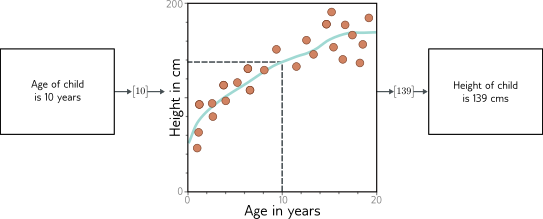
\includegraphics[width=\linewidth]{png/chapter1/IntroAgeHeight}
	\caption{机器学习是人工智能的一个分支,它专注于将数学模型应用于观测数据。它主要分为三个类别:监督学习、非监督学习和强化学习。深度神经网络在这三个领域中均发挥着重要作用。}
\end{figure}


\section{监督学习}
监督学习模型建立了一种从输入数据到输出预测的关系。在后续几节中,我们会详细探讨输入、输出、模型本身,以及“训练”模型所指的含义。

\subsection{回归和分类问题}
图 1.2 展示了几个回归和分类问题的例子。在每个例子中,都有一个与现实世界相关的输入(如一个句子、一段声音文件、一幅图片等),这些输入被转换成数字向量。这个向量就是模型的输入。模型把这个输入映射到一个输出向量,随后这个输出向量被再次转换,变成一个具有现实意义的预测。目前,我们主要关注输入和输出,并把模型当作一个黑盒子,它接受一个数字向量并输出另一个数字向量。

图 1.2a 中的模型基于如房屋的平方米数和卧室数量等输入特征来预测房价。这是一个回归问题,因为模型返回的是一个连续数值(而非某个类别)。而图 1.2b 中的模型则以分子的化学结构为输入,预测其熔点和沸点。由于预测了多个数值,这是一个多变量回归问题。

图 1.2c 中的模型接收包含餐厅评论的文本字符串作为输入,并预测评论是正面的还是负面的。这是一个二元分类问题,因为模型试图将输入分配到两个不同的类别中。输出向量包含输入属于每个类别的概率。图 1.2d 和 1.2e 则展示了多类别分类问题。在这里,模型将输入分配到多于两个的类别中。第一个例子中,输入是一个音频文件,模型预测它包含的音乐类型。第二个例子中,输入是一幅图片,模型预测图片中包含的对象。在这些例子中,模型均返回一个包含各类别概率的大小为 N 的向量。

\begin{figure}
	\centering
	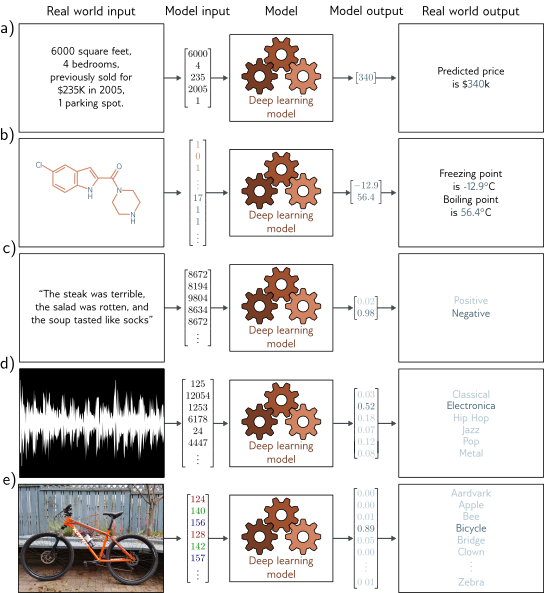
\includegraphics[width=0.7\linewidth]{png/chapter1/IntroModels}
	\caption{a)这个回归模型使用描述房产特征的数字向量来预测其价格。b)这个多变量回归模型以化学分子的结构为输入,预测其熔点和沸点。c)这个二元分类模型接收餐厅评论,并将其划分为正面或负面。d)这个多类别分类问题将一段音频片段归类为 N 种音乐类型中的一种。e)第二个多类别分类问题中,模型根据图片可能包含的 N 种物体之一来分类图片。}
\end{figure}

\subsection{输入}
图 1.2 中的输入数据类型各异。在房价预测例子中,输入是一个固定长度的向量,包含了描述房产特征的值。这是一种表格数据,它没有内在结构;如果我们改变输入值的顺序再构建一个新模型,预期模型的预测结果不会改变。

另一方面,在餐厅评论的例子中,输入是一段文本。这可能根据评论中的单词数而长度不同,且输入顺序很重要;例如,“我的妻子吃了鸡肉”与“鸡肉吃了我的妻子”意义截然不同。在传递给模型之前,文本必须被编码为数字形式。这里,我们使用一个包含 10,000 个词的固定词汇表,并将单词索引简单拼接起来。

在音乐分类的例子中,输入向量可能是固定大小的(比如 10 秒音频片段),但其维度非常高。数字音频通常以 44.1 kHz 采样并以 16 位整数表示,因此一个 10 秒的音频片段包含 441,000 个整数。显然,监督学习模型必须能够处理大量输入。图像分类例子中的输入(由每个像素的 RGB 值串联起来的)也非常庞大。而且,它的结构本质上是二维的;即使在输入向量中不相邻,上下相邻的两个像素也紧密相关。

最后,考虑预测分子熔点和沸点的模型的输入。一个分子可能包含不同数量且连接方式各异的原子。在这种情况下,模型需要同时考虑分子的几何结构和组成原子。
\subsection{机器学习模型}
到目前为止,我们把机器学习模型当作一个黑盒子,它接受输入向量并返回输出向量。但这个黑盒子里面究竟是什么呢?考虑一个根据孩子年龄来预测身高的模型(见图 1.3)。机器学习模型其实是一个数学方程,描述了平均身高如何随年龄变化(图 1.3 中的青色曲线)。当我们把年龄输入这个方程,它就会返回相应的身高。例如,如果年龄是 10 岁,我们预测身高为 139 厘米。

更精确地说,这个模型代表了一系列方程,用于将输入映射到输出(即不同的青色曲线)。特定的方程(曲线)是根据训练数据(输入和输出对的示例)来选择的。在图 1.3 中,这些对由橙色点表示,我们可以看到模型(青色线条)合理地描述了这些数据。当我们谈到训练或拟合一个模型时,我们的意思是在可能的方程(青色曲线)中寻找一个最能准确描述训练数据的关系。

\begin{figure}
	\centering
	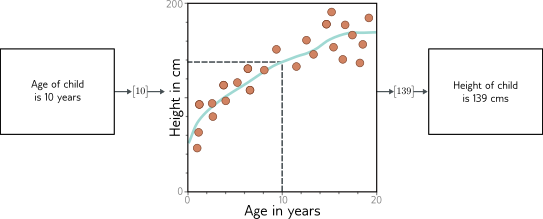
\includegraphics[width=0.7\linewidth]{png/chapter1/IntroAgeHeight}
	\caption{机器学习模型。该模型表示一系列关系,将输入(儿童年龄)与输出(儿童身高)联系起来。通过训练数据(橙色点,包括输入/输出对)来选定具体的关系。在训练模型过程中,我们寻找能够很好描述数据的关系。这里,经过训练的模型是青色曲线,可以用来计算任何年龄的儿童身高。}
\end{figure}

因此,图 1.2 中的模型需要标记好的输入/输出对来进行训练。例如,音乐分类模型需要大量音频片段,这些片段已由人类专家确定了各自的音乐类型。这些输入/输出对在训练过程中起到了教师或监督者的作用,这就是“监督学习”这个术语的由来。

\subsection{深度神经网络}
这本书着重讨论深度神经网络,这是一种特别有效的机器学习模型。它们是方程,能够代表输入和输出之间极其广泛的关系,并且在这些关系中寻找描述训练数据的关系特别容易。

深度神经网络可以处理非常大、变化多端的输入,并且能够包含各种内部结构。它们能输出单个实数(回归)、多个数值(多变量回归)或两个或更多类别的概率(分别对应二元和多类别分类)。正如我们在下一节中将看到的,它们的输出也可能非常大、变长,并且包含内部结构。想象具有这些特性的方程可能很困难,读者应努力暂时搁置怀疑。

\subsection{结构化输出}
图 1.4a 展示了一个用于语义分割的多变量二元分类模型。在这里,输入图像的每个像素都被分配一个二元标签,指示它是属于牛还是背景。图 1.4b 展示了一个多变量回归模型,输入是街景图像,输出是每个像素的深度。在这两种情况下,输出都是高维且有结构的。然而,这种结构与输入紧密相关,可以被利用;如果一个像素被标记为“牛”,那么具有相似 RGB 值的邻近像素可能有相同的标签。

图 1.4c-e 描述了三个输出具有与输入不太紧密相关的复杂结构的模型。图 1.4c 展示了一个模型,输入是音频文件,输出是文件中的转录词。图 1.4d 是一个翻译模型,输入是英文文本,输出是法文翻译。图 1.4e 描述了一个极具挑战性的任务,输入是描述性文本,模型需要生成与这个描述匹配的图像。

原则上,这三个后续任务可以在标准监督学习框架下解决,但它们更为困难,原因有二。首先,输出可能确实模糊不清;从英语到法语有多种有效翻译,任何描述都可能对应多种图像。其次,输出包含大量结构;并非所有单词串都能构成有效的英语和法语句子,也不是所有 RGB 值的组合都能构成合理的图像。除了学习映射,我们还必须遵循输出的“语法”。

\begin{figure}
	\centering
	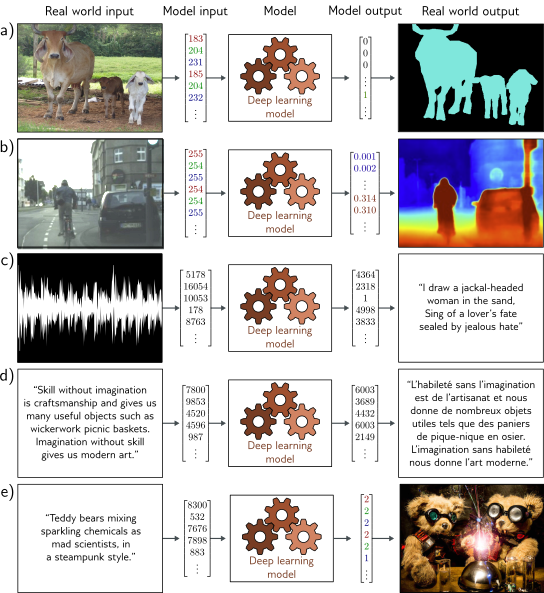
\includegraphics[width=0.7\linewidth]{png/chapter1/IntroModels2a}
	\caption{具有结构化输出的监督学习任务。a) 这个语义分割模型把 RGB 图像映射到一个二元图像,用于指示每个像素是属于背景还是牛(改编自 Noh 等人,2015年)。b) 这个单目深度估计模型将 RGB 图像映射到一个输出图像,每个像素代表深度(改编自 Cordts 等人,2016年)。c) 这个音频转录模型将音频样本映射到音频中所说话语的文字转录。d) 这个翻译模型将英语文本字符串映射到其对应的法语翻译。e) 这个图像合成模型将文字描述映射到一幅图像(示例来自 https://openai.com/dall-e-2/ )。在每个案例中,输出都具有复杂的内部结构或语法。在某些情况下,与输入相兼容的输出可能有多个。}
\end{figure}


幸运的是,这种“语法”可以在不需要输出标签的情况下学习。例如,我们可以通过学习大量文本数据的统计信息来学习构建有效的英语句子。这为本书接下来讨论的无监督学习模型部分提供了一个联系。

\section{无监督学习}
从没有对应输出标签的输入数据中构建模型被称为无监督学习;缺乏输出标签意味着不存在“监督”。无监督学习的目标不是学习输入到输出的映射,而是描述或理解数据的结构。就像监督学习一样,数据可能具有非常不同的特点;它可能是离散或连续的,低维或高维的,长度固定或变化的。

\subsection{生成式模型}
本书着重介绍生成式无监督模型,这类模型学习如何合成新的数据实例,使其在统计上与训练数据难以区分。一些生成式模型明确描述了输入数据的概率分布,并通过从这个分布中抽样来生成新实例。其他模型则仅学习生成新实例的机制,而不直接描述其分布。

最先进的生成式模型能够合成极为逼真但与训练实例不同的实例。它们在生成图像(见图 1.5)和文本(见图 1.6)方面特别成功。这些模型还可以在某些输出预先确定的约束下合成数据(称为条件生成)。例如,包括图像修复(见图 1.7)和文本补全(见图 1.8)在内的应用。事实上,现代文本生成模型非常强大,以至于它们看起来几乎具有智能。给定一段文本后接一个问题,模型通常能通过生成文档最可能的补全来“填补”缺失的答案。然而,实际上,模型只了解语言的统计特性,并不真正理解其答案的含义。

\begin{figure}
	\centering
	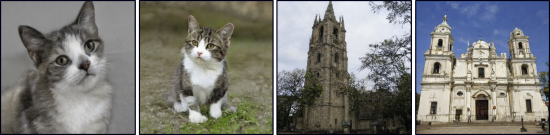
\includegraphics[width=0.7\linewidth]{png/chapter1/IntroSynthesis}
	\caption{图像生成式模型。左图:两幅图像由训练有素的猫图模型生成。这些不是真正的猫,而是概率模型生成的样本。右图:两幅图像由专门训练的建筑图模型生成。改编自 Karras 等人 (2020b)。}

\end{figure}

\begin{figure}
	\centering
	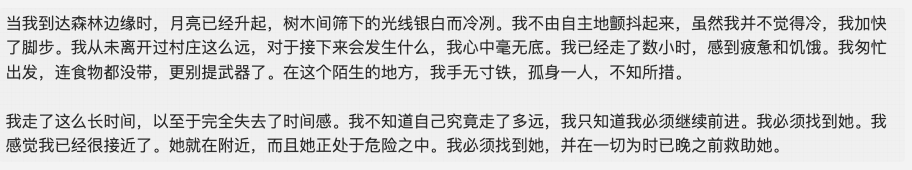
\includegraphics[width=0.7\linewidth]{png/chapter1/16}
	\caption{文本数据生成式模型合成的短篇故事。该模型描述了一个为每个输出字符串分配概率的概率分布。通过从模型中抽样,可以创造出遵循训练数据(这里是短篇故事)统计特性的字符串,这些字符串之前从未出现过。}
\end{figure}



\begin{figure}
	\centering
	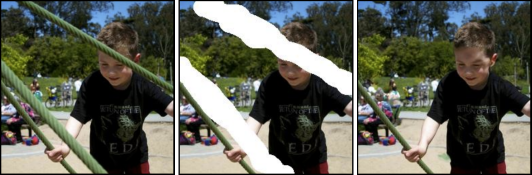
\includegraphics[width=0.7\linewidth]{png/chapter1/IntroCompletion}
	\caption{图像修复。原始图像(左图)中,男孩被金属缆绳遮挡。不需要的区域(中图)被移除,生成式模型在其余像素保持不变的约束下合成了新图像(右图)。改编自 Saharia 等人 (2022a)。}
\end{figure}

\begin{figure}
	\centering
	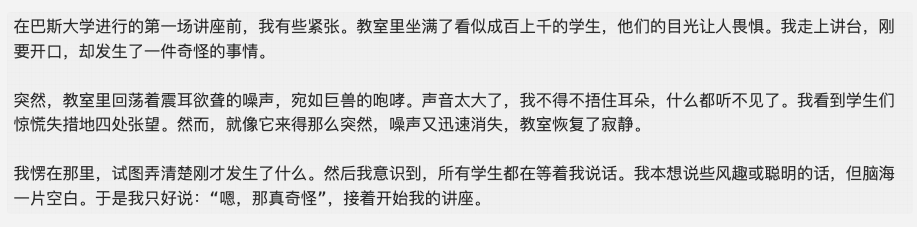
\includegraphics[width=0.7\linewidth]{png/chapter1/18}
	\caption{条件性文本合成。给定一段初始文本(第一段),文本生成式模型可以通过合成“缺失”的剩余部分来合理地继续这段文字。由 GPT3 生成(Brown 等人,2020)。}
\end{figure}


\subsection{潜变量}
一些生成式模型(但不是所有)利用了这样一个观点:数据的维度可以比原始观测变量的数量更小。例如,有效且有意义的英语句子的数量远少于随机组合单词形成的字符串数量。同样,真实世界的图像只占通过随机赋予每个像素 RGB 值能创建的图像的一小部分。这是因为图像是由物理过程生成的(见图 1.9)。

\begin{figure}
	\centering
	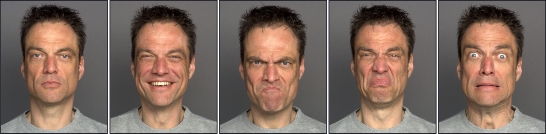
\includegraphics[width=0.7\linewidth]{png/chapter1/IntroFaceSpace}
	\caption{人脸的变化。人脸大约包含 42 块肌肉,因此可以用大约 42 个数字来描述同一个人在相同光照条件下的图像中的大部分变化。一般而言,图像、音乐和文本的数据集可以用相对较少的潜在变量来描述,尽管通常更难将这些变量与特定的物理机制联系起来。图像来自 Dynamic FACES 数据库(Holland 等人,2019)。}
\end{figure}

这就引出了一个想法,即我们可以使用较少的潜在变量来描述每个数据实例。在这里,深度学习的作用是描述这些潜变量与数据之间的映射关系。这些潜变量通常被设计为具有简单的概率分布。通过从这个分布中抽样并将结果通过深度学习模型传递,我们可以创造新的样本(见图 1.10)。

\begin{figure}
	\centering
	
\includegraphics[width=0.7\linewidth]{png/chapter1/IntroLatent}
	\caption{潜变量。潜变量在许多生成模型中扮演关键角色,这些模型利用深度学习来揭示低维潜变量与观测到的高维数据之间的联系。潜变量按设计拥有简易的概率分布。因此,通过从这些潜变量的简单分布中采样,再利用深度学习模型将采样结果映射到观测数据空间,我们便能创造出新的样本。}
\end{figure}


这些模型为操纵真实数据提供了新的方法。例如,考虑找出支持两个真实实例的潜变量。我们可以通过在它们的潜在表示之间插值,并将中间位置映射回数据空间,从而在这些实例之间进行插值(见图 1.11)。

\begin{figure}
	\centering
	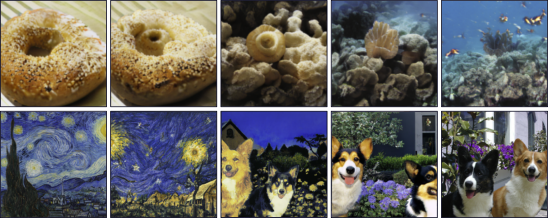
\includegraphics[width=0.7\linewidth]{png/chapter1/IntroInterpolate}
	\caption{图像插值。图像插值是一种有趣的应用。在每一行的图像中,左右两侧为真实图像,中间三张则是生成模型创造的插值序列。这些生成模型学习到了所有图像均可通过一组潜在变量来生成的原理。通过确定这两张真实图像的潜变量,对它们的值进行插值,然后用这些中间变量生成新图像,我们能创造出既视觉上合理,又融合了两张原始图像特征的中间图像。上排图片改编自 Sauer 等人 (2022),下排图片改编自 Ramesh 等人 (2022)。}
\end{figure}


\subsection{结合监督学习与无监督学习}
具有潜变量的生成式模型也可以促进输出具有结构的监督学习模型的发展(见图 1.4)。例如,考虑学习如何预测与描述相对应的图像。我们可以学习文本的潜变量与图像的潜变量之间的关系,而不是直接将文本输入映射到图像上。

这种方法有三个优点。首先,由于输入和输出维度较低,我们可能需要更少的文本/图像对来学习这种映射。其次,我们更有可能生成看起来合理的图像;潜变量的任何合理值都应该产生像是一个可信的示例。第三,如果我们在两组潜变量之间的映射或潜变量到图像的映射中引入随机性,那么我们可以生成多个都与描述相匹配的图像(见图 1.12)。

\begin{figure}
	\centering
	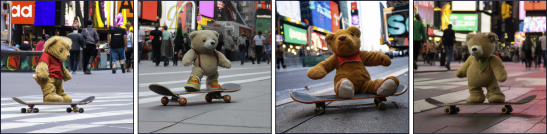
\includegraphics[width=0.7\linewidth]{png/chapter1/IntroVariety}
	\caption{从“时代广场上的滑板泰迪熊”这个标题出发,DALL·E-2(Ramesh 等人,2022)生成了多张图片。}
\end{figure}


\subsection{强化学习}
机器学习的最后一个领域是强化学习。这个范畴引入了代理(agent)的概念,代理生活在一个世界中,在每个时间步骤中可以执行特定行动。行动会改变系统的状态,但这种改变不一定是确定性的。执行行动还可能产生奖励,强化学习的目标是让代理学会选择能够平均获得高奖励的行动。

一个复杂点是奖励可能在行动后一段时间才出现,因此把奖励与特定行动关联起来并不直接。这被称为时间性信用分配问题。在学习过程中,代理必须在探索(寻找新的可能性)和利用(使用已知的策略)之间做出平衡;也许代理已经学会了如何获得适度的奖励,它应该继续遵循这个策略(利用现有知识),还是尝试不同的行动以寻找改进的机会(探索新的可能性)?
\subsection{两个例子}
考虑教一个类人机器人如何行走。机器人在特定时间可以执行有限的行动(如移动各种关节),这些行动会改变世界的状态(即它的姿态)。我们可以通过设立障碍赛道上的检查点来奖励机器人。为了到达每个检查点,它必须执行许多行动,但当收到奖励时,很难确定哪些行动对奖励有贡献,哪些是无关紧要的。这就是时间性信用分配问题的一个实例。

第二个例子是学习下棋。同样,代理在任何时刻都有一组有效的行动(棋子移动)。然而,这些行动以非确定性的方式改变系统状态;对于任何行动选择,对手可能以多种不同的方式回应。这里,我们可以根据捕获棋子来设定奖励结构,或者在游戏结束时赢得比赛来获得单一奖励。在后者情况下,时间性信用分配问题非常严重;系统必须学习在众多走法中哪些是成功或失败的关键。

探索与利用的权衡在这两个例子中也很明显。机器人可能已经发现,通过侧躺并用一条腿推动可以前进。这种策略虽然能让机器人移动并获得奖励,但比最优解——站立行走——要慢得多。因此,它面临一个选择,是利用已知的策略(沿地面滑行)还是探索其他可能的行动(可能实现更快的移动)。在下棋例子中也是如此,代理可能学到了一系列合理的开局走法。它应该利用这些知识,还是探索不同的开局序列?

深度学习如何融入强化学习框架可能不那么明显。有几种可能的方法,其中一种是使用深度网络构建从观察到的世界状态到行动的映射。这被称为策略网络。在机器人的例子中,策略网络会学习从传感器测量到关节运动的映射。在下棋的例子中,网络将学习从棋盘的当前状态到走法选择的映射(见图 1.13)。

\begin{figure}
	\centering
	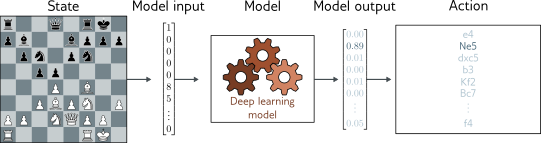
\includegraphics[width=0.7\linewidth]{png/chapter1/IntroReinforce}
	\caption{在强化学习中使用策略网络是一种创新。通过深度神经网络,我们可以定义从状态(例如棋盘上的位置)到动作(可能的移动)的映射。这种映射即为所谓的“策略”。}
\end{figure}


\section{伦理}
如果不讨论人工智能的伦理影响就撰写本书,将是不负责任的。这种强大技术将至少在与电力、内燃机、晶体管或互联网相同的程度上改变世界。在医疗保健、设计、娱乐、交通、教育以及几乎所有商业领域的潜在益处都是巨大的。然而,科学家和工程师对其工作成果的影响常常过于乐观,造成的潜在伤害同样巨大。以下几点突出了五个关注点。

\textbf{偏见与公平性}:如果我们训练一个系统基于历史数据来预测个人的薪酬水平,那么这个系统将重现历史偏见;例如,它可能会预测女性应获得比男性更低的薪酬。已有几个此类案例成为国际新闻:一个用于超分辨率人脸图像的 AI 系统使非白人看起来更白;一个用于生成图像的系统在被要求合成律师图片时只产生了男性的图片。不慎使用 AI 进行算法决策可能会加剧现有偏见。有关更多讨论,请参阅 Binns(2018)。


\textbf{解释性}:深度学习系统做出决策,但我们通常不知道其基于何种信息或如何做出的。它们可能包含数十亿个参数,我们无法仅通过检查来理解它们的工作原理。这导致了可解释 AI 的子领域的形成。一个中等成功的领域是产生局部解释;我们无法解释整个系统,但可以提供为何做出特定决策的可解释描述。然而,目前尚不清楚是否有可能构建对其用户甚至其创建者完全透明的复杂决策系统。更多信息请参见 Grennan 等人(2022)。


\textbf{武器化 AI}:所有重要技术都被直接或间接地用于战争。可悲的是,暴力冲突似乎是人类行为的不可避免特征。AI 可能是有史以来构建的最强大的技术,并且无疑会在军事背景中得到广泛部署。事实上,这已经在发生(参见 Heikkilä,2022)。


\textbf{集中权力}:世界上最强大的公司之所以大力投资人工智能,并非出于改善人类命运的善意兴趣。他们意识到这些技术将使他们获得巨大利润。与任何先进技术一样,深度学习可能会使权力集中在掌握它的少数组织手中。将目前由人类完成的工作自动化,将改变经济环境,对薪资较低、技能较少的工人的生计产生不成比例的影响。乐观主义者认为,工业革命期间也发生了类似的变革,导致工作时间缩短。但事实是,我们不知道 AI 的大规模应用将对社会产生何种影响(参见 David,2015)。


\textbf{存在风险}:人类面临的主要存在风险都来自技术。气候变化是由工业化推动的。核武器源于物理学研究。由于交通、农业和建筑的创新,使得人口更大、更密集、更相互连接,疫情因此更易发生且传播更快。人工智能带来新的存在风险。我们应该非常谨慎地构建比人类更有能力和可扩展性的系统。在最乐观的情况下,它会将巨大的权力集中在少数拥有者手中。在最悲观的情况下,我们可能无法控制它,甚至无法理解其动机(参见 Tegmark,2018)。

这份列表远非完整。AI 还可能助长监控、虚假信息、隐私侵犯、欺诈和金融市场操纵的现象,而且培训 AI 系统所需的能源也会对气候变化产生影响。此外,这些担忧并非无的放矢;AI 的伦理问题已有许多实例(参见 Dao,2021年的部分列表)。互联网的近期历史展示了新技术可能以意想不到的方式造成伤害。80年代和90年代初的在线社区几乎无法预见假新闻、垃圾邮件、网络骚扰、欺诈、网络欺凌、极端单身文化、政治操纵、个人信息泄露、网络激进化和网络报复色情的泛滥。

研究或学习(或撰写关于)AI 的每个人都应思考科学家对其技术使用的责任程度。我们应该认识到,资本主义是推动 AI 发展的主要动力,法律进步和社会利益的实施可能会大大落后。我们应反思作为科学家和工程师,是否有可能控制这个领域的进展,以减少潜在的伤害。我们还应考虑愿意为哪种组织工作。他们在减少 AI 潜在危害方面的承诺有多认真?他们是否只是为了减少声誉风险而进行“伦理洗白”,还是真正实施机制来停止伦理上可疑的项目?


鼓励所有读者进一步探索这些问题。在线课程 \\
\url{https://ethics-of-ai.mooc.fi/} 是一个有用的入门资源。如果您是使用本书进行教学的教授,建议您与学生讨论这些问题。如果您是在未进行此类讨论的课程中学习的学生,请敦促您的教授实现这一点。如果您在企业环境中部署或研究 AI,建议您审视雇主的价值观,并帮助改变它们(或离开),如果它们不尽人意。

\section{本书结构}
本书的结构遵循本导言的框架。第2至9章详细介绍监督学习流程。我们描述了浅层和深层神经网络,并讨论了如何训练它们、如何衡量和提高它们的性能。第10至13章讲述了深度神经网络的常见架构变化,包括卷积网络、残差连接和变压器,这些架构在监督学习、无监督学习和强化学习中都有应用。

第14至18章聚焦通过深度神经网络进行的无监督学习。我们专门为四种现代深度生成模型各写了一章:生成对抗网络、变分自编码器、规范化流和扩散模型。第19章简要介绍深度强化学习。这个主题本可以轻易成为一本书的核心,因此本书的处理相对浅显。然而,这一部分旨在为不熟悉这一领域的读者提供一个良好的起点。

尽管本书标题为“深度学习”,但深度学习的某些方面仍然缺乏充分理解。第20章提出了一些基础问题:为什么深度网络易于训练?为什么它们泛化能力如此强?为什么需要如此多的参数?它们是否需要深度?在此过程中,我们探讨了一些意外现象,如损失函数的结构、双重下降、理解和彩票。书籍以第21章结尾,讨论伦理和深度学习。
\section{其他书籍}
这本书是自成体系的,但主要聚焦于深度学习领域。它旨在成为《深度学习》(Goodfellow 等人,2016年)的精神续作,后者是一本极佳的资源,但没有涵盖近期的进展。对于更广泛的机器学习领域,最新且百科全书式的资源是《概率机器学习》(Murphy,2022年、2023年)。然而,《模式识别与机器学习》(Bishop,2006年)仍是一本优秀且相关的书籍。

如果你喜欢本书,那么我之前的作品《计算机视觉:模型、学习与推理》(Prince,2012年)也值得一读。尽管部分内容已显陈旧,但它包含了对概率的全面介绍,包括贝叶斯方法,以及潜变量模型、计算机视觉的几何学、高斯过程和图形模型的良好初步覆盖。它使用与本书相同的符号,并可以在网上找到。关于图形模型的详细处理可以在《概率图形模型:原理与技术》(Koller \& Friedman,2009年)中找到,而高斯过程则由《机器学习中的高斯过程》(Williams \& Rasmussen,2006年)涵盖。

对于背景数学,可以参考《机器学习的数学》(Deisenroth 等人,2020年)。更注重编程的方法可以参考《深入深度学习》(Zhang 等人,2023年)。计算机视觉最佳概述是 Szeliski(2022年),还有即将出版的《计算机视觉基础》(Torralba 等人,2024年)。学习图神经网络的好起点是《图表示学习》(Hamilton,2020年)。关于强化学习的权威著作是《强化学习导论》(Sutton \& Barto,2018年)。一个很好的入门资源是《深度强化学习基础》(Graesser \& Keng,2019年)。

\section{如何阅读本书}
本书的大多数剩余章节包含主要正文、注释部分和一组问题。主要正文旨在自成体系,可在不参考章节其他部分的情况下阅读。尽可能地,背景数学被纳入正文中。但对于那些可能会分散主要论点注意力的更大主题,背景材料被放在附录中,并在页边提供参考。本书中的大多数符号是标准的。但一些约定使用得不太广泛,鼓励读者在继续之前查阅附录A。

正文包括许多深度学习模型和结果的新颖插图和可视化。我努力提供现有观点的新解释,而不仅仅是整理他人的工作。深度学习是一个新领域,有时现象理解不足。我试图明确指出在哪些情况下是这样,以及何时我的解释应该谨慎对待。

只有在描述结果的章节主体中才包含参考文献。相反,它们可以在章节末尾的注释部分找到。我在主文中通常不尊重历史先例;如果当前技术的祖先已不再有用,我将不会提及它。然而,该领域的历史发展在注释部分有所描述,并希望公平地分配了功劳。注释被组织成段落,并提供了进一步阅读的指引。它们应该帮助读者在子领域内定位自己,并理解它与机器学习的其他部分的关系。注释部分不像正文那样自成体系。根据您的背景知识和兴趣水平,您可能会觉得这些部分更有用或更没用。

每章都有一些相关的问题。它们在主文的边栏中被引用,应在相应的点尝试解答。正如乔治·波利亚所指出的,“你看,数学不是一项观赏运动。”他是正确的,我强烈建议你在阅读时尝试解决问题。在某些情况下,它们提供了将帮助您理解正文的洞察。在相关网站上提供答案的问题用星号标记。此外,帮助您理解本书中观点的 Python 笔记本也可通过网站获得,并在正文的边栏中引用。事实上,如果您感到生疏,现在可能值得通读一下有关背景数学的笔记本。

不幸的是,AI 研究的进展速度使得这本书不可避免地成为一项持续的工作。如果有您觉得难以理解的部分、值得注意的遗漏或看似多余的部分,请通过相关网站与我联系。我们可以一起让下一版更好。


\chapter{监督学习}

监督学习模型就是将一个或多个输入转化为一个或多个输出的方式。比如,我们可以将某部二手丰田普锐斯的车龄和行驶里程作为输入,预估的车辆价格则是输出。

这个模型其实只是个数学公式;当我们把输入放入这个公式进行计算,我们得到的结果就是所谓的“推理”。这个公式还包含一些参数。改变参数值会改变计算的结果;这个公式其实描述了输入和输出之间所有可能关系的“家族”,而参数则定义了其中的特定关系。

每当我们训练或学习模型时,我们其实是在寻找可以真实反映输入与输出关系的参数。学习算法收集一组输入/输出对,然后调整这些参数,使得输入数据能够尽可能准确地预测出其相应的输出。如果对于这些训练数据,模型的预测效果不错,那么我们就会寄希望于它能在未来遇到新的未知输出的情况下,依然能做出好的预测。

本章的目标是深入探讨这些观点。我们会首先对这个框架进行更详细的描述,并引入一些专业的符号。然后,我们会用一个简单的范例来展示如何使用一条直线来描述输入与输出间的关系。这个线性模型比较容易理解且直观,却恰好包含了所有有监督学习的关键概念。

\section{监督学习介绍}

在监督学习中,我们的目标是建立一个模型,这个模型能够接收输入 x 并给出预测结果 y。简单来说,我们假设输入 x 和输出 y 都是预先定义且大小固定的向量,并且这些向量中的元素排列顺序始终一致。举个例子,如普锐斯汽车的例子,输入 x 总是先包含汽车的年龄,然后是行驶里程,按照这个顺序。这种数据被称为结构化或表格数据(structured or tabular data)。

为了进行预测,我们需要一个函数模型 f[•],它以 x 为输入并返回预测结果 y,即:

\begin{equation}
y = f[x] 
\end{equation}

当我们根据输入 x 来计算预测结果 y 时,这个过程称为推理(inference)。

这个模型实际上是一个具有固定形式的数学方程,代表了输入和输出之间各种不同的关系。模型中也包含一些参数 $\phi$。这些参数的选择决定了输入和输出之间具体的关系。更准确地说,我们应该这样表达这个关系:

\begin{equation}
y = f[x, \phi] 
\end{equation}

当我们谈及学习或训练模型时,意味着我们在尝试找出能够根据输入合理预测输出的参数 $\phi$。我们通过一组包含 I 对输入和输出样本 ${x_i, y_i}$ 的训练数据集来学习这些参数。我们的目标是选取能够尽可能准确地将每一个训练输入映射到它对应的输出的参数。我们通过损失函数 L 来衡量这种映射的准确程度。损失函数是一个标量值,它概括了模型基于当前参数 $\phi$ 预测训练数据输出与实际输入的不匹配程度。

我们可以把损失函数视为参数的函数 $L[\phi]$。在训练模型时,我们的目标是寻找一组参数 $\hat \phi$,这组参数能够使损失函数的值最小:

\begin{equation}
\hat \phi = \arg \mathop{\min}\limits_{\phi} L [\phi] 
\end{equation}

如果在这个最小化过程之后损失很小,说明我们找到了一组能够从训练输入 $x_i$ 准确预测训练输出 $y_i$ 的模型参数。

在训练模型之后,我们接下来需要评估它的性能。我们会在一组独立的测试数据上运行模型,以评估它对于训练过程中未曾见过的示例的泛化能力。如果模型的性能达到预期,那么我们就可以开始部署这个模型了。

\section{线性回归示例}

让我们通过一个简单的实例,将这些理论概念具体化。假设有一个模型 $y = f[x, \phi]$,它能够根据某个输入 x,预测出单一的输出 y。接着,我们将构建一个损失函数,并就如何训练这个模型进行讨论。

\subsection{一维线性回归模型}

一维线性回归模型以一条直线的形式,展现了输入x和输出y之间的关系:

\begin{align}
y &= f[x, \phi] \notag \\
&= \phi_0 + \phi_1 x 
\end{align}


这个模型有两个参数 $\phi = [\phi_0,\phi_1]^T$,$\phi_0$ 和 $\phi_1$ 分别代表直线的截距和斜率。调整截距和斜率的值,可以改变输入和输出之间的关系(如图 2.1 所示)。因此,我们可以认为方程 2.4 描述的是一族可能的输入-输出关系(即:所有可能的线)。而具体选择哪个参数,就能确定这一族关系中的特定成员(也就是特定的一条直线)。

\begin{figure}
	\centering
	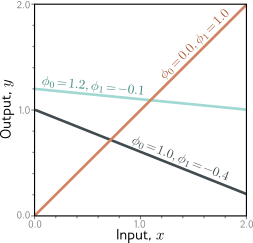
\includegraphics[width=0.7\linewidth]{png/chapter2/SupervisedLinear}
	\caption{线性回归模型。在我们确定了参数 $\phi = [\phi_0 , \phi_1 ]^T$ 的选择后,该模型就可以依据输入值(x轴位置)来预测输出值(y轴位置)。通过调整y轴截距 $\phi_0$ 和直线斜率 $\phi_1$ 的值,我们的预测结果(代表为青色、橙色以及灰色线)也就有所不同。所以,线性回归模型(公式 2.4)实际上就定义了一个输入/输出关系的集合(代表为多条直线),而模型的参数则用来确定我们将使用的具体一条直线(即集合中的一个成员)。}
\end{figure}


\subsection{损失(Loss)}

对于这个模型,训练数据集(见图 2.2a)由 I 对输入/输出数据对 ${x_i, y_i}$ 组成。图 2.2b–d 展示了三组不同参数定义下的三条线。图 2.2d 中的绿色线条比其他两条更准确地描述了数据,因为它更接近于数据点。然而,我们需要一种系统的方法来判断哪一组参数 $\phi$ 比其他参数更优。为了做到这一点,我们给每一组参数赋予一个数值,这个数值表示模型与数据之间不匹配的程度。我们称这个值为损失;损失越低,表示模型拟合得越好。

这种不匹配是通过模型预测 $f[x_i,\phi]$(线在 xi 处的高度)和真实输出 $y_i$ 之间的差异来表示的。在图 2.2b–d 中,这些差异以橙色虚线显示。我们通过计算所有 I 对训练数据对中这些差异的平方和来量化总的不匹配、训练误差或损失:

\begin{align}
	L(\phi) &= \sum_{i=1}^{I} (f(x_i; \phi) - y_i)^2  \notag \\
	&= \sum_{i=1}^{I} (\phi_0 + \phi_1 x_i - y_i)^2 
\end{align}


由于最佳参数是使这个表达式最小化的参数,我们称之为最小二乘损失。平方操作意味着偏差的方向(即线是在数据点上方还是下方)不重要。我们将在第 5 章回到这个选择的理论原因。

损失 L 是参数 $\phi$ 的函数;当模型拟合较差时(如图 2.2b,c),损失会较大;而拟合良好时(如图 2.2d),损失则较小。从这个角度来看,我们称 $L[\phi]$ 为损失函数或成本函数。目标是找到能最小化这个量的参数 $\hat \phi$:


\begin{align}
	\hat{\phi} &= \underset{\phi}{\mathrm{argmin}} \, L(\phi) \notag \\ 
	&= \underset{\phi}{\mathrm{argmin}} \, \left[ \sum_{i=1}^{I} (f(x_i; \phi) - y_i)^2 \right] \notag \\ 
	&= \underset{\phi}{\mathrm{argmin}} \, \left[ \sum_{i=1}^{I} (\phi_0 + \phi_1 x_i - y_i)^2 \right]  
\end{align} 


由于模型只有两个参数(y 截距 $\phi_0$ 和斜率 $\phi_1$),我们可以为每一组参数值的组合计算损失,并将损失函数以表面的形式进行可视化(见图 2.3)。"最佳" 参数则位于这个表面的最低点。

\begin{figure}
	\centering
	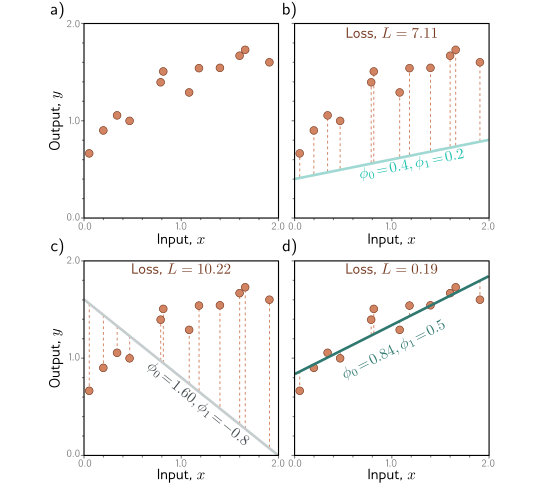
\includegraphics[width=0.7\linewidth]{png/chapter2/SupervisedLinearFitError}
	\caption{线性回归中的训练数据,模型和损失的展示。a)我们的训练数据(标注为橙色的点)包含着 I = 12 个输入输出对 {$x_i , y_i$ }。b–d)每一部分都展示了一个具有不同参数的线性回归模型。根据我们选择的截距和斜率参数 $\phi = [\phi_0 , \phi_1 ]^T$,模型的预测结果(表示为橙色的虚线)的误差可能会变大或变小。这里的损失 L 实际上就是这些误差的平方和。如果你看一下图表 b 和 c,你会发现其线条拟合的并不是很好,这使得它们的损失 L 分别为 7.07 和 10.28,这是相当大的损失。而在图表 d 中,该模型拟合得相当好,导致其损失 L 仅为 0.20;实际上,这就是所有可能的线条中损失最小的那一条,可以认为这些参数是最优的。}

\end{figure}

\begin{figure}
	\centering
	\includegraphics[width=0.7\linewidth]{png/chapter2/SupervisedSurface}
	\caption{}
\end{figure}

\begin{figure}
	\centering
	\includegraphics[width=0.7\linewidth]{png/chapter2/SupervisedOpt}
	\caption{}
\end{figure}

\subsection{训练}

寻找使损失最小化的参数的过程称为模型拟合、训练或学习。这个过程的基本方法是首先随机选择初始参数,然后通过不断“下降”损失函数,直到找到最低点(参见图 2.4)。具体做法是,测量当前位置损失函数表面的梯度,然后朝最陡峭的下坡方向迈出一步。接着不断重复这个过程,直到梯度变平,无法再进一步优化。

\subsection{测试}

当模型训练完成后,我们想知道它在实际应用中的表现。这可以通过在一组独立的测试数据上计算损失来实现。模型预测的准确性在多大程度上能泛化到测试数据,一方面取决于训练数据的代表性和完整性;另一方面,则取决于模型的表达能力。例如,简单的模型如直线可能无法完全捕捉输入和输出之间的真实关系,这就是所谓的欠拟合。相反,表达能力过强的模型可能会描述训练数据中的一些不典型的统计特性,导致不正常的预测结果,这被称为过拟合。

\section{总结}

监督学习模型是一个函数 $y = f[x, \phi]$,它将输入 x 与输出 y 关联起来。这种特定的关系由参数 \(\phi\) 决定。为了训练模型,我们在训练数据集 {$x_i, y_i$} 上定义了损失函数 $L[\phi]$,以量化模型预测 $f[x_i,\phi]$ 与实际观测输出 yi 之间的不匹配程度。然后我们寻找能够最小化这个损失的参数。我们通过在不同的测试数据集上评估模型,来检查它对新输入的泛化能力。

接下来的第 3-9 章将进一步深入这些概念。首先,我们将探讨模型本身。1D 线性回归的明显限制是,它只能以直线形式描述输入和输出之间的关系。第 3 章介绍的浅层神经网络虽然比线性回归稍复杂,但能描述更广泛的输入/输出关系。第 4 章的深度神经网络在保持表达能力的同时,能用更少的参数描述复杂函数,且在实际应用中表现更佳。

第 5 章将探讨不同任务下的损失函数及其理论基础,特别是最小二乘损失。第 6 章和第 7 章将讨论训练过程,第 8 章将讨论如何衡量模型性能,而第 9 章将考察旨在提高性能的正则化技术。

\section{Notes}

\textbf{损失函数(loss Function)与成本函数(cost function)}:在机器学习领域,尤其是在本书中,“损失函数”和“成本函数”这两个术语通常可以互换使用。但更准确地说,损失函数是指与单个数据点相关的具体项(例如,方程 2.5 中每个平方项),而成本函数是指需要被最小化的整体量(即方程 2.5 中的整个右侧部分)。成本函数可能还包含与单个数据点无关的其他项(详见第 9.1 节)。更广义上,目标函数指的是任何需要最大化或最小化的函数。

\textbf{生成(Generative)模型与判别(Discriminative)模型}:本章中提到的模型 $y = f[x, \phi]$ 属于判别模型。这类模型基于实际测量的数据 x 来预测输出 y。另一种方法是构建生成模型 $x = g[y, \phi]$,在这种模型中,实际测量的数据 x 被看作是输出 y 的函数。
虽然生成模型的缺点是它们不直接预测 y,但它们的优势在于能够融入关于数据生成方式的先验知识。比如,如果我们要预测图像 x 中汽车的三维位置和方向 y,我们可以在函数 $x = g[y, \phi]$ 中加入关于汽车形状、三维几何和光传输的知识。
尽管这听起来是个好主意,但实际上,在现代机器学习中,判别模型更为主流。这是因为在生成模型中利用先验知识所带来的优势通常不及利用大量训练数据来学习灵活的判别模型所获得的优势。

\section{习题}

\textbf{问题 2.1} 为了在损失函数(方程 2.5)上实现“downhill”,我们需要计算它对参数 $\phi_0$ 和 $\phi_1$ 的梯度。请计算出这两个参数的梯度值 $\partial L / \partial \phi_0$ 和 $\partial L / \partial \phi_1$ 的具体表达式。

\textbf{问题 2.2} 请证明我们可以通过将问题 2.1 中的导数设置为零,然后求解 $\phi_0$ 和 $\phi_1$,以闭合形式找到损失函数的最小值。需要注意的是,这种方法适用于线性回归,但不适用于更复杂的模型;这就是为什么我们通常会使用迭代的模型拟合方法,例如梯度下降(参见图 2.4)。

\textbf{问题 2.3} 考虑将线性回归改造为生成模型,形式为 $x = g[y, \phi] = \phi_0 + \phi_1 y$。请问这种情况下的新损失函数是什么?请找出进行推理所需的逆函数 $y = g^{-1}[x, \phi]$ 的表达式。对于一个给定的训练数据集 {${x_i,y_i}$},这个模型是否会做出与判别模型版本相同的预测?一种验证方法是编写程序,使用这两种方法对三个数据点进行线性拟合,看结果是否一致。
\chapter{浅层神经网络}

第二章我们学习了使用一维线性回归的监督学习方法,但这种模型只能表示出输入与输出之间简单的线性关系。在这一章里,我们将接触到浅层神经网络。这种网络可以表达分段线性函数,并且能力强大到足以近似任何复杂度的多维输入和输出之间的关系。
\section{神经网络示例}
浅层神经网络是带有参数 \(\phi\) 的函数 \(y = f[x, \phi]\),它将多变量输入 \(x\) 映射成多变量输出 \(y\)。关于浅层神经网络的全面定义将在第3.4节中给出。首先,我们通过一个示例网络 \(f[x, \phi]\) 来介绍核心概念。这个网络能够将单一变量输入 \(x\) 转化为单一变量输出 \(y\),并包含十个参数 \(\phi = \{\phi_0, \phi_1, \phi_2, \phi_3, \theta_{10}, \theta_{11}, \theta_{20}, \theta_{21}, \theta_{30}, \theta_{31}\}\):


\begin{align}
	y &= f[x, \phi] \\ 
	&= \phi_0 + \phi_1a[\theta_{10} + \theta_{11}x] + \phi_2a[\theta_{20} + \theta_{21}x] + \phi_3a[\theta_{30} + \theta_{31}x] \tag{3.1}
\end{align}


这个计算过程可以分成三个步骤:首先,计算输入数据 \(x\) 的三个线性函数(\(\theta_{10} + \theta_{11}x, \theta_{20} + \theta_{21}x, \theta_{30} + \theta_{31}x\))。接着,将这三个函数的结果通过激活函数 \(a[\cdot]\) 处理。最后,用 \(\phi_1, \phi_2, \phi_3\) 对这三个激活结果进行加权,求和,并加上一个偏移量 \(\phi_0\)。

接下来,我们需要定义激活函数(activation function)\(a[\cdot]\)。虽然有很多选择,但最常用的是整流线性单元(ReLU):

\[
a[z] = ReLU[z] = 
\begin{cases}
	0 & \text{if } z < 0 \\
	z & \text{if } z \geq 0
\end{cases} \tag{3.2}
\]

这个函数在输入为正时返回输入值,否则返回零(参见图 3.1)。

\begin{figure}[h!]
	\centering
	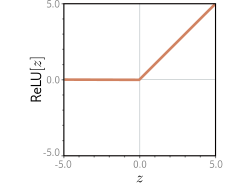
\includegraphics[width=0.7\linewidth]{png/chapter3/ShallowReLU.png}
\caption{图 3.1 整流线性单元 (Rectified Linear Unit, ReLU)。这种激活函数在输入小于零时输出为零,否则保持输入值不变。简而言之,它将所有负数输入值变为零。需要注意的是,虽然有许多其他激活函数可供选择(参见图 3.13),但 ReLU 由于其简单易懂,成为最常用的选择。}
\end{figure}

方程 3.1 描述了哪一类输入/输出关系可能不是一目了然的。但是,前一章节提到的所有概念都适用于这里。方程 3.1 表示了一个函数族,具体的函数取决于 φ 中的十个参数。如果我们知道这些参数,就可以通过对给定输入 \(x\) 计算该方程来进行推断(预测 \(y\))。给定一个训练数据集 \(\{{x_i,y_i}\}^I_{i=1}\),我们可以定义一个最小二乘损失函数 \(L[\phi]\),用它来评估对于任意参数值 \(\phi\),模型描述该数据集的效果。为了训练这个模型,我们要找出能够最小化这个损失的参数值 \(\hat \phi\)。


\subsection{神经网络直观理解}
事实上,方程 3.1 描述了一个连续分段线性函数族(见图 3.2),这个函数族最多包含四个线性区域。下面我们解析这个方程,阐释它是如何描绘出这样一个函数族的。为了便于理解,我们将这个函数拆分为两个部分。首先,我们定义几个中间量:


\begin{align}
	h1 = a[\theta_{10} + \theta_{11}x] \\
	h2 = a[\theta_{20} + \theta_{21}x] \\
	h3 = a[\theta_{30} + \theta_{31}x]  \tag{3.3}
\end{align} 

这里的 \(h1, h2, h3\) 被称为隐藏单元。然后,我们通过将这些隐藏单元与一个线性函数结合来计算输出:

\[
y = \phi_0 + \phi_1h1 + \phi_2h2 + \phi_3h3 \tag{3.4}
\]

图 3.3 展示了形成图 3.2a 中函数的计算流程。每个隐藏单元内包含了一个关于输入的线性函数 \(\theta_0 + \theta_1x\),该线性函数在零点以下被 ReLU 函数 \(a[\cdot]\) 截断。这三条线在零点交叉的位置形成了最终输出函数的三个“拐点”。然后,分别用 \(\phi_1, \phi_2, \phi_3\) 对这三条被截断的线加权。最后,加上偏移量 \(\phi_0\) 来控制最终函数的整体高度。

\begin{figure}[h!]
	\centering
	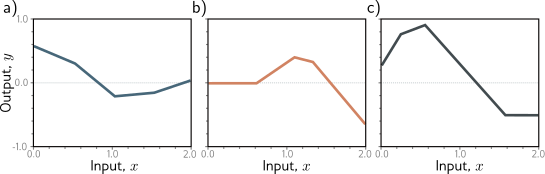
\includegraphics[width=0.7\linewidth]{png/chapter3/ShallowFunctions.png}
\caption{图 3.2 由方程 3.1 定义的函数族。a-c) 展示了三种不同参数 \(\phi\) 的选择下的函数。在这些函数中,输入与输出的关系均为分段线性。不过,各个拐点的位置、拐点间线段的斜率,以及整体高度各不相同。}
\end{figure}

\begin{figure}[h!]
	\centering
	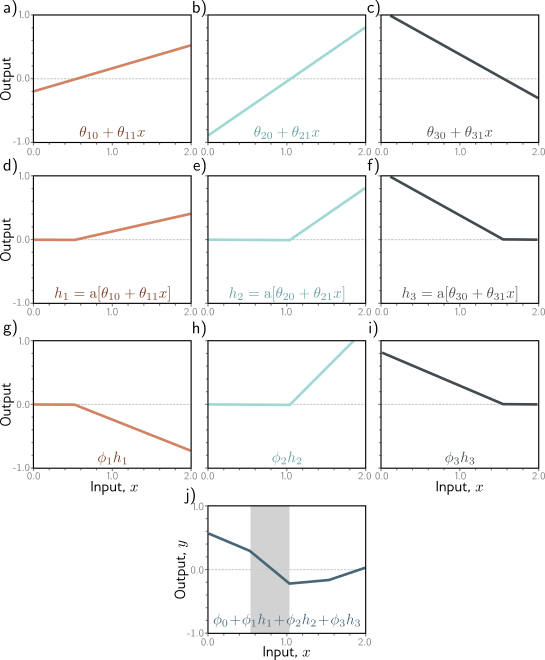
\includegraphics[width=0.7\linewidth]{png/chapter3/ShallowBuildUp.png}
\caption{展示图 3.2a 中函数的计算过程。a-c) 输入 x 分别经过三个具有不同 y 截距 θ•0 和斜率 θ•1 的线性函数处理。d-f) 每个线性函数的输出再经过 ReLU 激活函数处理,将所有负数输出值变为零。g-i) 接着,这三个处理过的输出分别乘以权重 \(\phi_1 , \phi_2 , \phi_3\) 进行加权。j) 最后,将这些加权后的输出相加,并加上一个控制整体高度的偏移量 \(\phi_0\) 。每个线性段代表了隐层单元中的一种不同激活模式。在阴影区域,h2 处于非激活状态(被剪切),而 h1 和 h3 保持激活状态。}
\end{figure}

在图 3.3j 中,每个线性区域对应于隐藏单元中的一种不同激活模式。当一个单元在 ReLU 函数下被截断时,我们称其为不活跃状态;相反,如果没有被截断,则处于活跃状态。例如,在阴影区域内,得到 \(h1\) 和 \(h3\)(处于活跃状态)的贡献,但没有 \(h2\)(处于不活跃状态)的贡献。每个线性区域的斜率取决于两个因素:(i)这个区域内活跃输入的原始斜率 \(\theta_1\) 和(ii)随后应用的权重 \(\phi\)。例如,在阴影区域(参见问题 3.3),斜率是 \(\phi_1\theta_{11} + \theta_{31}\phi_3\),其中第一项是图中(g)面板的斜率,第二项是(i)面板的斜率。

由于每个隐藏单元贡献了一个拐点,所以有三个隐藏单元时,可以形成四个线性区域。但是,这些区域的斜率只有三个是相互独立的;第四个斜率要么是零(如果在这个区域所有隐藏单元都处于不活跃状态),要么是其他区域斜率的总和。
\subsection{描绘神经网络}
我们此前一直探讨的是一种神经网络,它由一个输入层、一个输出层和三个隐藏单元组成。在图 3.4a 中,我们将这个网络形象化。图中,最左边的是输入层,中间部分是隐藏单元,右边则是输出层。图中的每一条连接线代表了这个神经网络的十个参数中的一个。而为了图像表示的简洁,我们通常不会特别标出截距参数,所以大多数情况下,这个网络的表达方式如图 3.4b 所示。

\begin{figure}[h!]
	\centering
	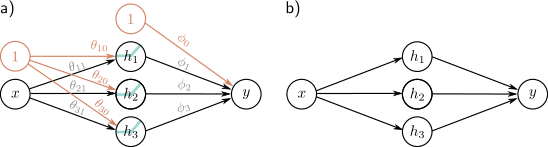
\includegraphics[width=0.7\linewidth]{png/chapter3/ShallowNet.png}
\caption{图 3.4 描述神经网络结构。a) 输入变量 x 位于左侧,隐层单元 h1 , h2 , 和 h3 位于中间,输出变量 y 位于右侧。计算过程从左向右进行。输入变量用于计算隐层单元的值,这些隐层单元的组合进而生成输出值。图中的十个箭头分别代表一个参数,橙色代表截距,黑色代表斜率。每个参数将其来源的值乘以自己,然后将结果加到其目标上。例如,我们将参数 φ1 与来源于 h1 的值相乘,再将结果加到 y 上。为了将偏移量纳入这一计算框架,引入了值为 1 的额外节点(橙色圆圈),例如我们将 φ0 乘以 1(实际上无变化)后加到 y 上。ReLU 函数被应用于隐层单元。b) 通常情况下,网络图中会省略截距、ReLU 函数和参数名称的显示;这种简化后的表示方式实际上描述了同一个网络。}
\end{figure}

\section{通用逼近定理(Universal approximation theorem)}
在上一节中,我们介绍了一个只有一个输入、一个输出、使用ReLU激活函数,并配备了三个隐藏单元的神经网络示例。现在,让我们稍微扩展这个概念,考虑一个拥有 \(D\) 个隐藏单元的网络,其中第 \(d^{th}\) 个隐藏单元表示为:

\[
h_d = a[\theta_{d0} + \theta_{d1}x], \tag{3.5}
\]

这些隐藏单元通过线性方式结合,共同产生输出:


\[
y = \phi_0 + \sum_{d=1}^{D} \phi_dh_d. \tag{3.6}
\]

在浅层网络中,隐藏单元的数量是衡量网络“容量”(即其处理复杂性的能力)的一个指标。当使用 ReLU 激活函数时,具有 \(D\) 个隐藏单元的网络输出最多有 \(D\) 个拐点,因此它是一个最多有 \(D + 1\) 个线性区域的分段线性函数。随着增加更多的隐藏单元,模型能够逼近更为复杂的函数。

实际上,如果网络有足够的“容量”(即足够多的隐藏单元),它就能够以任意精度描述定义在实数线某个紧凑子集上的任何连续一维函数。这是因为,每当我们增加一个隐藏单元,就会在函数中增加一个新的线性区域。随着这些线性区域的增多,它们代表了函数中越来越小的部分,这些部分可以被一条线越来越精确地逼近(参见图 3.5)。通用逼近定理证明了,对于任何连续函数,都存在一个浅层网络,它能以任意设定的精度逼近这个函数。

\section{多变量输入与输出}
在前述例子中,网络仅有一个单变量标量输入 \(x\) 和一个单变量标量输出 \(y\)。然而,对于网络将多变量输入 \(x = [x_1, x_2, \dots, x_{D_i}]^T\)(其中 “\(^T\)” 表示转置)映射到多变量输出预测 \(y = [y_1, y_2, \dots, y_{D_o}]^T\) 的更广泛情况,通用逼近定理 (universal approximation theorem) 依然成立。我们首先探讨如何改进模型以预测多变量输出。接着,我们将讨论多变量输入的处理方式。最后,在第 3.4 节,我们会提出浅层神经网络的通用定义。
\section{多变量输入和输出}
在前面的例子中,网络有一个单变量输入 \(x\) 和一个单变量输出 \(y\)。然而,通用逼近定理也同样适用于网络将多变量输入 \(x = [x_1, x_2, \dots, x_{D_i}]^T\) 映射到多变量输出 \(y = [y_1, y_2, \dots, y_{D_o}]^T\) 的更一般情况。我们首先探索如何将模型扩展到预测多变量输出。然后我们会考虑多变量输入。最后,在第3.4节中,我们将提出浅层神经网络的通用定义。
\subsection{可视化多变量输出}
为了将网络扩展到能产生多变量输出 \(y\),我们可以简单地为每个输出使用隐藏单元的不同线性函数。例如,一个具有单变量输入 \(x\)、四个隐藏单元 \(h_1, h_2, h_3, h_4\) 和一个二维多变量输出 \(y = [y_1, y_2]^T\) 的网络可以定义为:


\begin{align}
	h_1 = a[\theta_{10} + \theta_{11}x] \\
	h_2 = a[\theta_{20} + \theta_{21}x] \\
	h_3 = a[\theta_{30} + \theta_{31}x] \\
	h_4 = a[\theta_{40} + \theta_{41}x]  \tag{3.7}
\end{align} 

以及

\begin{align}
	y1 = \phi_{10} + \phi_{11}h1 + \phi_{12}h2 + \phi_{13}h3 + \phi_{14}h4 \\
	y2 = \phi_{20} + \phi_{21}h1 + \phi_{22}h2 + \phi_{23}h3 + \phi_{24}h4. \tag{3.8}
\end{align} 


这两个输出是隐藏单元的两种不同线性组合。

如图 3.3 所示,分段函数的“接点”取决于隐藏单元处的 ReLU 函数 \(a[\cdot]\) 截断的初始线性函数 \(\theta_0 + \theta_1x\)。由于 \(y1\) 和 \(y2\) 都是相同四个隐藏单元的不同线性函数,因此它们各自的四个“接点”位置必须相同。然而,这些线性区域的斜率和整体的垂直偏移可能不同(参见图 3.6)。

\begin{figure}[h!]
	\centering
	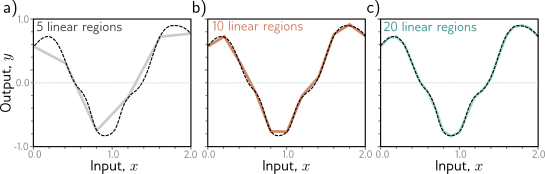
\includegraphics[width=0.7\linewidth]{png/chapter3/ShallowApproximate.png}
\caption{图 3.5 用分段线性模型近似一维函数(虚线表示)。a-c) 随着分段区域的数量增加,该模型逐渐趋近于连续函数。一个只有单一输入的神经网络会为每个隐层单元新增一个线性区域。根据通用近似定理(Universal Approximation Theorem),只要隐层单元足够多,就能构建一个浅层神经网络,该网络能够以任意精度近似定义在 RDi 紧凑子集上的任何连续函数。}
\end{figure}

\begin{figure}[h!]
	\centering
	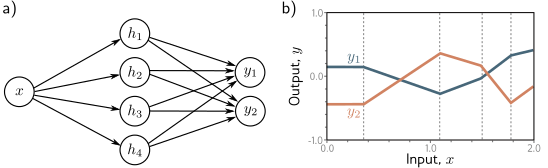
\includegraphics[width=0.7\linewidth]{png/chapter3/ShallowNetTwoOutputs.png}
\caption{图 3.6 展示了一个具有一个输入、四个隐层单元和两个输出的网络。a) 网络结构的可视化展示。b) 该网络产生两个分段线性函数,y1[x] 和 y2[x]。由于这些函数共享相同的隐层单元,它们的四个“关节”(位于垂直虚线处)位置是固定的,但它们的斜率和整体高度可能有所不同。}
\end{figure}

\begin{figure}[h!]
	\centering
	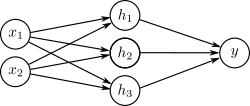
\includegraphics[width=0.7\linewidth]{png/chapter3/ShallowNetTwoInputs.png}
\caption{图 3.7 展示了具有二维多变量输入 $x = [x1, x2]^T$ 和单一输出 y 的神经网络的可视化。}
\end{figure}

\subsection{可视化多变量输入}

为了应对多变量输入 \(x\),我们扩展了输入与隐藏单元之间的线性关联。例如,一个有两个输入 \(x = [x_1, x_2]^T\) 和一个标量输出 \(y\) 的网络(参见图 3.7)可能由三个隐藏单元构成,定义如下:


\begin{align}
	h1 = a[\theta_{10} + \theta_{11}x_1 + \theta_{12}x_2] \\
	h2 = a[\theta_{20} + \theta_{21}x_1 + \theta_{22}x_2] \\
	h3 = a[\theta_{30} + \theta_{31}x_1 + \theta_{32}x_2] \tag{3.9}
\end{align} 



这里,每个输入都对应一个斜率参数。隐藏单元以通常的方式结合,形成输出:

\[
y = \phi_0 + \phi_1h1 + \phi_2h2 + \phi_3h3 \tag{3.10}
\]


图 3.8 展示了这个网络的处理过程。每个隐藏单元接收两个输入的线性组合,这在三维输入/输出空间中形成了一个有方向的平面。激活函数将这些平面的负值剪切为零。接着,这些被剪切的平面在第二个线性函数(方程 3.10)中被重新组合,形成了一个由凸多边形区域组成的连续分段线性表面(见图 3.8j)。每个区域代表了一种不同的激活模式。例如,在中央的三角形区域中,第一个和第三个隐藏单元处于激活状态,而第二个则未激活。当模型有超过两个输入时,可视化变得更加困难。不过,其基本原理是相似的:输出将是输入的连续分段线性函数,其中线性区域在多维输入空间中呈现为凸多面体。

需要注意的是,随着输入维度的增加,线性区域的数量迅速增长(参见图 3.9)。为了更好地理解这种增长速度,考虑每个隐藏单元定义了一个超平面,区分了单元活跃和不活跃的空间部分(见图 3.8d-f 中的青色线条)。如果我们的隐藏单元数量与输入维度 \(D_i\) 相等,我们可以将每个超平面与一个坐标轴对齐(见图 3.10)。对于两个输入维度,这会将空间划分为四个象限。对于三个维度,这会形成八个八分区,而对于 \(D_i\) 维度,则会形成 \(2^{D_i}\) 个正交空间。由于浅层神经网络通常比输入维度有更多的隐藏单元,它们通常会创造出超过 \(2^{D_i}\) 个线性区域。

\begin{figure}[h!]
	\centering
	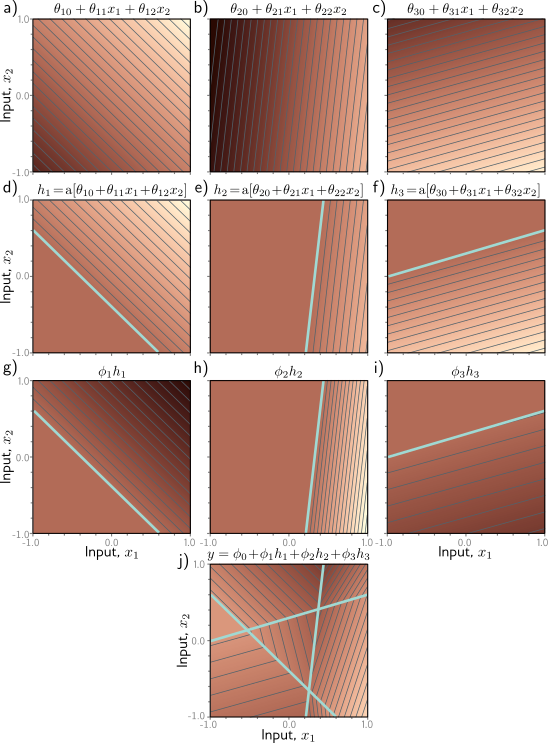
\includegraphics[width=0.7\linewidth]{png/chapter3/ShallowBuildUp2D.png}
\caption{图 3.8 在一个具有两个输入 \(x = [x1,x2]^T\)、三个隐层单元 h1,h2,h3 和一个输出 y 的网络中的处理过程。a-c) 每个隐层单元的输入是两个输入变量的线性函数,对应于一个方向性平面。亮度代表函数的输出,例如,在面板 (a) 中,亮度表示 \(θ_10 + θ_{11}x_1 + θ_{12} x2\)。细线代表等值线。d-f) ReLU (Rectified Linear Unit) 激活函数对每个平面进行剪切处理(青色线相当于图 3.3d-f 中的“关节”)。g-i) 这些被剪切的平面随后被加权,j) 然后和一个决定表面整体高度的偏移量相加。最终得到的是一个由凸的分段线性多边形区域构成的连续表面。}
\end{figure}

\begin{figure}[h!]
	\centering
	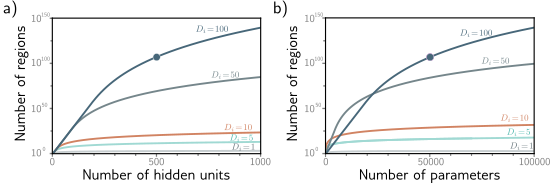
\includegraphics[width=0.7\linewidth]{png/chapter3/ShallowRegions.png}
\caption{图 3.9 隐层单元与线性区域的关系。a) 对于五种不同输入维度 Di = {1, 5, 10, 50, 100},展示了隐层单元数与其能够产生的最大线性区域数之间的关系。在高维度下,线性区域的数量迅速增加;例如,在 D = 500 单元和输入维度 Di = 100 的情况下,线性区域的数量可以超过 $10^107$(实心圆所示)。b) 将相同的数据以参数数量作为函数进行绘制。实心圆表示与 a) 面板中相同的模型,拥有 D = 500 隐层单元。这个网络有 51,001 个参数,在现代标准下被认为非常小。}
\end{figure}

\section{浅层神经网络:一般情况}

我们已经通过几个示例来展示浅层网络的工作原理。现在我们定义一个浅层神经网络的通用方程 \( y = f[x, \phi] \),它利用 \( h \in \mathbb{R}^{D_h} \) 个隐藏单元将多维输入 \( x \in \mathbb{R}^{D_i} \) 映射到多维输出 \( y \in \mathbb{R}^{D_o} \)。每个隐藏单元的计算方式如下:

\[
h_d = a \left[ \theta_{d0} + \sum_{i=1}^{D_i} \theta_{di}x_i \right] \tag{3.11}
\]


这些隐藏单元被线性方式组合,以产生输出:

\[
y_j = \phi_{j0} + \sum_{d=1}^{D_h} \phi_{jd}h_d \tag{3.12}
\]

其中 \(a[\cdot]\)  是一种非线性激活函数。该模型的参数为 \(\phi = \{ \theta_{\cdot}, \phi_{\cdot}\}\)。图 3.11 展示了一个包含三个输入、三个隐藏单元和两个输出的示例。

激活函数使得模型能描述输入与输出之间的非线性关系,因此它本身必须是非线性的;如果没有激活函数,或使用线性激活函数,从输入到输出的映射将被限制为线性映射。已尝试了多种不同的激活函数(见图 3.13),但最常用的选择是 ReLU(见图 3.1),它具有易于理解的优点。使用 ReLU 激活的网络将输入空间划分为由 ReLU 函数中的“接点”计算出的超平面交叉定义的凸多面体。每个凸多面体内包含一个不同的线性函数。尽管每个输出的多面体都相同,但它们包含的线性函数可能会有所不同。

\begin{figure}[h!]
	\centering
	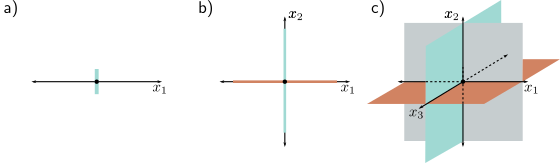
\includegraphics[width=0.7\linewidth]{png/chapter3/ShallowHyperplanes.png}
\caption{图 3.10 输入维度与线性区域数量的关系。a) 对于单输入维度的模型,一个隐层单元可以创建一个分割点,将输入轴分为两个线性区域。b) 在两个输入维度的模型中,两个隐层单元可以使用两条线(此处与坐标轴对齐)划分输入空间,形成四个区域。c) 在三个输入维度的模型中,三个隐层单元可以用三个平面(同样与坐标轴对齐)划分输入空间,形成八个区域。延伸这一逻辑,一个具有 Di 输入维度和 Di 隐层单元的模型可以用 Di 超平面来划分输入空间,从而形成 $2^Di$ 个线性区域。}
\end{figure}

\begin{figure}[h!]
	\centering
	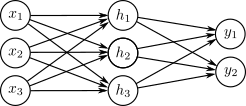
\includegraphics[width=0.7\linewidth]{png/chapter3/ShallowNetThreeInputsTwoOutputs.png}
\caption{图 3.11 展示了一个具有三个输入和两个输出的神经网络的可视化。该网络共有二十个参数,包括十五个斜率(由箭头指示)和五个偏移(未显示)。}
\end{figure}

\begin{figure}[h!]
	\centering
	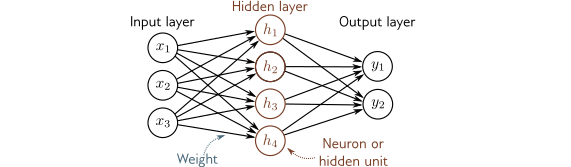
\includegraphics[width=0.7\linewidth]{png/chapter3/ShallowTerminology.png}
\caption{图 3.12 术语: 一个浅层网络由一个输入层、一个隐层和一个输出层构成。每一层都通过前向连接(箭头所示)与下一层相连,因此这类模型被称为前向网络(feed-forward networks)。当每一层中的每个变量都与下一层的每个变量相连时,我们称之为全连接网络(fully connected network)。每个连接代表了底层方程中的斜率参数,这些参数称为权重(weights)。隐层中的变量被称为神经元(neurons)或隐层单元(hidden units)。进入隐层单元的值称为激活前值(pre-activations),而隐层单元上的值(即应用 ReLU 函数后的值)称为激活值(activations)。}
\end{figure}

\section{术语}
在本章的结尾,我们来介绍一些术语。神经网络领域有很多专业术语。通常情况下,它们是通过层来描述的。在图 3.12 中,左边是输入层,中间是隐藏层,右边是输出层。我们可以说图 3.12 中的网络有一个包含四个隐藏单元的隐藏层。隐藏单元本身有时也被称为神经元。当数据通过网络传输时,隐藏层输入的值(即在应用 ReLU 函数之前的值)被称为预激活值。隐藏层的值(即在应用 ReLU 函数之后的值)被称为激活值。

由于历史原因,任何至少有一个隐藏层的神经网络也被称为多层感知器(MLP)。本章所述的具有一个隐藏层的网络有时被称为浅层神经网络。具有多个隐藏层的网络(将在下一章中描述)被称为深度神经网络。其中连接形成一个无环图(即没有循环的图,如本章中的所有示例)的神经网络被称为前馈网络。如果一个层中的每个元素都连接到下一个层中的每个元素(如本章中的所有示例),则该网络被称为全连接网络。这些连接代表了基础方程中的斜率参数,并被称为网络权重。偏移参数(在图 3.12 中未显示)被称为偏置。

\section{总结}
浅层神经网络包含一个隐藏层。它们的工作过程包括:(i) 计算输入的多个线性函数,(ii) 将这些函数结果通过激活函数处理,然后 (iii) 将这些激活后的结果线性组合以产生输出。浅层神经网络通过将输入空间划分成连续的、由分段线性区域组成的表面来根据输入 x 进行预测 y。只要拥有足够多的隐藏单元(神经元),浅层神经网络能够以任意精度逼近任何连续函数。

第 4 章将讨论深度神经网络,这些网络通过增加更多隐藏层来扩展本章所述的模型。第 5 至 7 章将描述如何训练这些模型。

\section{Notes}

\textbf{"神经"网络}:如果本章中的模型仅仅是函数,为什么它们被称为“神经网络”呢?这个连接实际上是比较脆弱的。像图 3.12 中的可视化包括节点(输入、隐藏单元和输出),它们之间有密集的连接。这与哺乳动物大脑中密集连接的神经元在表面上有相似之处。然而,几乎没有证据表明大脑计算的方式与神经网络相同,而且从生物学角度来考虑这一点是没有帮助的。

\textbf{神经网络的历史}:1943年,McCulloch 和 Pitts 首次提出了人工神经元的概念,这种神经元能够将输入信号组合以产生输出,但缺乏有效的学习算法。1958年,Rosenblatt 开发出了感知机(Perceptron),一种通过线性组合输入信号并设定阈值来做出是/否决策的模型,并为其设计了一种从数据中学习权重的算法。1969年,Minsky 和 Papert 指出,仅用线性函数处理一般分类问题是不够的。他们认为,通过增加带有非线性激活函数的隐藏层(由此产生了“多层感知机(Multi-layer Perceptron)”这一术语),可以学习到更广泛的输入/输出关系。不过,他们也指出,Rosenblatt 的算法无法学习这些模型的参数。直到20世纪80年代,一个有效的学习算法——反向传播(Backpropagation,详见第7章)才被发明,此后神经网络的研究才重新获得显著发展。关于神经网络历史的详细记载可参见 Kurenkov (2020)、Sejnowski (2018) 和 Schmidhuber (2022) 的著作。

\textbf{激活函数}:ReLU(Rectified Linear Unit)函数最早在1969年由 Fukushima 提出并使用。然而,在神经网络的早期阶段,更常见的激活函数是逻辑 S 形(Logistic Sigmoid)或双曲正切(Tanh)函数(见图 3.13a)。2009年以后,由 Jarrett et al.、Nair \& Hinton 和 Glorot et al. 等人的工作重新推广,ReLU 成为现代神经网络成功故事的重要组成部分。ReLU 的一个显著特性是,对于大于零的输入值,其输出相对于输入的导数恒为1,这有助于提高训练的稳定性和效率(详见第7章)。这与逻辑 S 形激活函数形成鲜明对比,后者的导数在大的正输入和负输入下会趋近于零,即发生饱和现象。

然而,ReLU函数存在一个明显的不足:当输入为负值时,它的导数为零。这意味着如果所有训练样本对某个ReLU函数都产生负输入,那么在训练过程中就无法改进该ReLU的输入参数。因为相对于输入权重的梯度在局部呈平坦状态,我们无法通过梯度下降法“下坡”。这种现象被称为ReLU消亡问题。为解决这一问题,提出了多种ReLU的改进版本(见图 3.13b),包括 (i) 渗漏ReLU(Leaky ReLU,Maas et al., 2013),即使对负输入值也有一定的线性输出,其斜率较小,大约为0.1;(ii) 参数化ReLU(Parametric ReLU,He et al., 2015),将负值部分的斜率作为一个可学习的参数;以及 (iii) 连接型ReLU(Concatenated ReLU,Shang et al., 2016),它生成两个输出,一个在零以下截断(类似于标准ReLU),另一个在零以上截断。

此外,还研究了多种平滑函数(见图 3.13c–d),例如soft-plus函数(Glorot et al., 2011)、高斯误差线性单元(Gaussian Error Linear Unit,Hendrycks \& Gimpel, 2016)、S形线性单元(Sigmoid Linear Unit,Hendrycks \& Gimpel, 2016)和指数线性单元(Exponential Linear Unit,Clevert et al., 2015)。这些函数大多旨在避免ReLU消亡问题,同时限制负值的梯度过大。Klambauer et al. (2017) 提出了缩放指数线性单元(Scaled Exponential Linear Unit,见图 3.13e),这一激活函数特别有趣,因为当输入方差在有限范围内时,它能帮助稳定激活值的方差(详见第7.5节)。2017年,Ramachandran et al. 采用了一种经验方法来选择激活函数。他们在可能的函数空间中寻找,在各种监督学习任务上表现最佳的函数。他们找到的最佳函数是 \(a[x] = x/(1 + exp[−βx])\),其中 β 是一个可学习的参数(见图 3.13f)。他们将这个函数命名为Swish。有趣的是,Swish实际上是对 Hendrycks \& Gimpel (2016) 和 Elfwing et al. (2018) 之前提出的激活函数的再发现。2019年,Howard et al. 提出了HardSwish函数,它近似于Swish,形状非常相似,但计算速度更快:

\[
HardSwish[z] =
\begin{cases} 
	0 & \text{for } z < -3 \\
	\frac{z(z + 3)}{6} & \text{for } -3 \leq z \leq 3 \\
	z & \text{for } z > 3 
\end{cases} \tag{3.13}
\]

尽管这些激活函数各有特点,但目前尚无定论哪种在实际应用中明显优于其他。不过,渗漏ReLU、参数化ReLU和许多连续函数在特定情况下相比ReLU确实表现出了轻微的性能提升。在本书剩余部分,我们主要关注使用基本ReLU函数的神经网络,因为它们创建的函数更容易根据线性区域数量进行刻画。

\textbf{通用逼近定理}:该定理的宽度版本指出,存在一个单隐藏层且隐藏单元数量有限的网络,能够在 Rn 的紧凑子集上以任意精度逼近任何特定的连续函数。这一理论最初由 Cybenko (1989) 针对 S 形激活函数类别证明,并后由 Hornik (1991) 扩展到更广泛的非线性激活函数。

\textbf{线性区域数量}:考虑一个拥有 \(D_i \geq 2\) 维输入和 D 个隐藏单元的浅层网络。其线性区域的数量取决于由 ReLU 函数的转折点所形成的 D 个超平面的相交情况(如图 3.8d-f 所示)。每个区域由 ReLU 函数对输入的剪切或不剪切的不同组合产生。Zaslavsky (1975) 指出,在 \(D_i \leq D\) 维输入空间内,由 D 个超平面所创造的区域数量最多可以达到 \(\sum_{j=0}^{D_i} \binom{D}{j}\)(即二项式系数之和)。一般而言,浅层神经网络的隐藏单元数 D 几乎总是大于输入维度 \(D_i\),并能在 \(2^{D_i}\) 到 \(2^D\) 之间创造多个线性区域。

\textbf{线性、仿射与非线性函数}:严格定义下,线性变换 \(f[\cdot]\) 是遵循叠加原理的任何函数,即  \(f[a + b] = f[a] + f[b]\)。根据这个定义,\(f[2a] = 2f[a]\)。加权和 \(f[h1, h2, h3] = \phi_{h1} + \phi_{h2} + \phi_{h3}\) 是线性的,但加上偏移(偏置)后,\(f[h1, h2, h3] = \phi_0 + \phi_{h1} + \phi_{h2} + \phi_{h3}\),就不再是线性的。例如,当我们加倍前一个函数的参数时,输出也加倍,但后一个函数不是这样。后者更恰当地被称为仿射函数。在机器学习领域,这些术语常常混用。在本书中,我们也将遵循这一习惯,把这两种函数都称为线性。我们将遇到的所有其他函数都是非线性的。


\begin{figure}[h!]
	\centering
	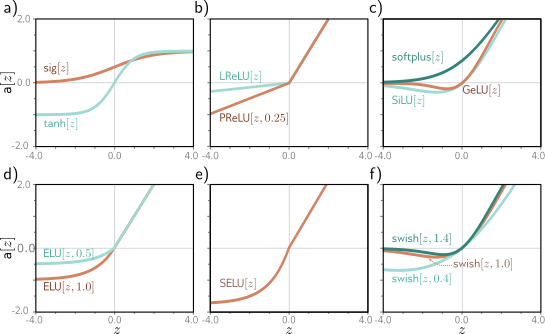
\includegraphics[width=0.7\linewidth]{png/chapter3/ShallowActivations.png}
\caption{图 3.13 激活函数(Activation functions)。a) Logistic sigmoid 函数和 tanh 函数。b) Leaky ReLU 函数和参数为 0.25 的 Parametric ReLU 函数。c) SoftPlus 函数、高斯误差线性激活函数(Gaussian error linear unit)和 sigmoid线性激活函数(sigmoid linear unit)。d) 参数为 0.5 和 1.0 的指数线性激活函数(Exponential Linear Unit)。e) 按比例调整的指数线性激活函数(Scaled Exponential Linear Unit)。f) 参数为 0.4,1.0,和 1.4 的 Swish 函数。}
\end{figure}

\begin{figure}[h!]
	\centering
	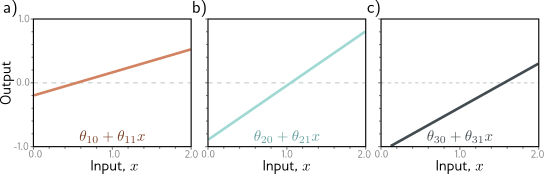
\includegraphics[width=0.7\linewidth]{png/chapter3/ShallowChangeSlope.png}
\caption{图 3.14:针对问题 3.4, 描述了一个网络的处理过程,该网络具有一个输入,三个隐藏单元,以及一个输出。a-c) 所示的是,每个隐藏单元接受的输入来源是原输入的线性转换。前两个隐藏单元接收到的输入与图 3.3 中的一样,但是最后一个与它们不同。}
\end{figure}

\section{课后习题}
\textbf{问题 3.1} 若方程 3.1 中的激活函数是线性的,即 \(a[z] = \phi_0 + \phi_{1}z\),则输入到输出的映射将是怎样的?如果移除激活函数,使 \(a[z] = z\),又将产生何种映射?

\textbf{问题 3.2} 在图 3.3j 的四个线性区域中,分别指出哪些隐藏单元是活跃的,哪些是不活跃的(即剪切或不剪切输入的隐藏单元)。

\textbf{问题 3.3} 导出图 3.3j 函数中“关节”位置的表达式,用十个参数 \(\phi\) 和输入 x 表示。同时,导出四个线性区域斜率的表达式。

\textbf{问题 3.4} 绘制图 3.3 的一个版本,其中第三个隐藏单元的截距和斜率发生变化,如图 3.14c 所示,假定其他参数保持不变。


\textbf{问题 3.5} 证明以下性质对于 \(\alpha \in \mathbb{R}^+\) 成立:
\[
ReLU[\alpha \cdot z] = \alpha \cdot ReLU[z] \tag{3.14}
\]
这是 ReLU 函数的非负齐次性质。

\textbf{问题 3.6} 继续问题 3.5,当我们将方程 3.3 和 3.4 中定义的浅层网络的参数 \(\theta_{10}\) 和 \(\theta_{11}\) 乘以一个正常数 \(\alpha\) 并将斜率 \(\phi_1\) 除以同一参数 \(\alpha\) 时,会发生什么?如果 \(\alpha\) 是负数呢?

\textbf{问题 3.7} 考虑使用最小二乘损失函数拟合方程 3.1 中的模型。这个损失函数是否有唯一的最小值?即,是否存在一组“最佳”参数?

\textbf{问题 3.8} 考虑将 ReLU 激活函数替换为 (i) 海维赛德阶跃函数 \(heaviside[z]\),(ii) 双曲正切函数 \(tanh[z]\),以及 (iii) 矩形函数 \(rect[z]\)。为每种激活函数重绘图 3.3,并简要描述使用一个输入、三个隐藏单元和一个输出的神经网络,对于每种激活函数所能创造的函数族。
\[
heaviside[z] = \begin{cases}
	0 & z < 0 \\
	1 & z \geq 0
\end{cases}
\]
\[
rect[z] = \begin{cases}
	0 & z < 0 \\
	1 & 0 \leq z \leq 1 \\
	0 & z > 1
\end{cases} \tag{3.15}
\]

请针对以下每一个函数,重新绘制一份图 3.3。原始的参数为:\(\phi = [\phi_0, \phi_1, \phi_2, \phi_3, \theta_{10}, \theta_{20}, 	\theta_{30}, 	\theta_{31}] = [-0.23, -1.3, 1.3, 0.66, -0.2, 0.4, -0.9, 0.9, 1.1, -0.7]\)。对于每个激活函数,尝试用通俗的语言解释一下,对于那些神经网络来说,它们只有一个输入,三个隐藏单元和一个输出,可以创造出什么样的函数族。


\textbf{问题 3.9} 证明图 3.3 中第三个线性区域的斜率是第一个和第四个线性区域斜率之和。

\textbf{问题 3.10} 考虑一个有一个输入、一个输出和三个隐藏单元的神经网络。图 3.3 展示了如何形成四个线性区域。在什么情况下,这个网络会产生少于四个线性区域的分段线性函数?

\textbf{问题 3.11} 和 \textbf{问题 3.12} 图 3.7 中的模型包含多少个参数?

\textbf{问题 3.13} 在图 3.8 的七个区域中,每个区域的激活模式分别是什么?也就是说,在每个区域中,哪些隐藏单元是激活状态(传递输入),哪些是非激活状态(剪切输入)?

\textbf{问题 3.14} 描述图 3.11 中网络的方程。需要三个方程从输入计算出三个隐藏单元的值,以及两个方程从隐藏单元计算输出。

\textbf{问题 3.15} 图 3.11 中的网络最多能创建多少个三维线性区域?

\textbf{问题 3.16} 描述一个具有两个输入、四个隐藏单元和三个输出的网络的方程,并按照图 3.11 的风格绘制这个网络模型。

\textbf{问题 3.17} 方程 3.11 和 3.12 定义了一个具有 \(D_i\) 个输入、\(D_h\) 个隐藏单元的隐藏层以及 \(D_o\) 个输出的通用神经网络。求出模型参数数量的表达式,以 \(D_i\)、\(D_h\) 和 \(D_o\) 作为变量。

\textbf{问题 3.18} 证明一个只有 \(D_i = 2\) 维输入、\(D_o = 1\) 维输出和 \(D = 3\) 个隐藏单元的浅层网络所能创建的最大区域数是七个,如图 3.8j 所示。根据 Zaslavsky (1975) 的结果,即用 \(D\) 个超平面划分 \(D_i\) 维空间时创造的最大区域数是 \(\sum_{j=0}^{D_i} \binom{D}{j}\)。如果在这个模型中增加两个隐藏单元,使 \(D = 5\),那么最大区域数将是多少?


\chapter{深度神经网络}
前面一章我们讨论了只有一个隐藏层的浅层神经网络。本章,我们将转向深度神经网络,这种网络拥有多个隐藏层。无论是浅层还是深层网络,当使用 ReLU (Rectified Linear Unit) 激活函数时,它们都能实现从输入到输出的分段直线式的变换。

浅层神经网络的能力随着隐藏单元数量的增加而提升。实际上,如果隐藏单元足够多,这些网络甚至能够模拟高维空间中极其复杂的函数。但是,对于某些特定的函数,所需的隐藏单元数量可能非常庞大,以至于实际应用变得不现实。相比之下,深度神经网络能够在相同数量的参数条件下创造出更多的线性判断区域。因此,从实际应用的角度来看,深度网络能够描述更加广泛的函数类型。

\section{组合神经网络}
为了更深入地理解深度神经网络的行为特征,我们首先考虑将两个浅层网络进行组合,使得第一个网络的输出成为第二个网络的输入。设想两个各有三个隐藏单元的浅层网络(见图 4.1a)。第一个网络接收输入 x,并产生输出 y,其定义如下:

\begin{align}
h_1 = a[\theta_{10}+\theta_{11}x] \notag \\
h_2 = a[\theta_{20}+\theta_{21}x] \notag \\
h_3 = a[\theta_{30}+\theta_{31}x] 
\end{align} 

以及
\begin{equation}
y = \phi_0 + \phi_1h_1 + \phi_2h_2 + \phi_3h_3 
\end{equation}
第二个网络以 y 作为输入,产生输出 \(y \prime\),定义如下:

\begin{align}
h^\prime_1 = a[\theta^\prime_{10}+\theta^\prime_{11}y] \notag \\
h^\prime_2 = a[\theta^\prime_{20}+\theta^\prime_{21}y] \notag \\
h^\prime_3 = a[\theta^\prime_{30}+\theta^\prime_{31}y] 
\end{align} 


以及
\begin{equation}
y^\prime = \phi^\prime_0 + \phi^\prime_1h^\prime_1 + \phi^\prime_2h^\prime_2 + \phi^\prime_3h^\prime_3 
\end{equation}
在使用 ReLU(线性整流单元)激活函数的情况下,该模型描述了一系列分段线性函数。然而,与拥有六个隐藏单元的浅层网络相比,这种组合网络的线性区域数量潜在地更多。例如,若第一个网络产生三个正负斜率交替的区域(见图 4.1b),这意味着三个不同范围的 x 值被映射到同一输出范围 \(y \in [−1, 1]\)。接下来,从该 y 范围到 \(y \prime\) 的映射被重复应用三次。最终的效果是,第二个网络定义的函数被复制三次,从而形成九个线性区域。这一原理在更高维度同样适用(见图 4.2)。


组合网络的另一种思考方式是,第一个网络将输入空间 x 折叠回自身,使得多个输入产生相同的输出。随后,第二个网络在所有重叠点上应用同一函数,实现了函数在这些点上的复制(见图 4.3)。

\begin{figure}[ht!]
	\centering
	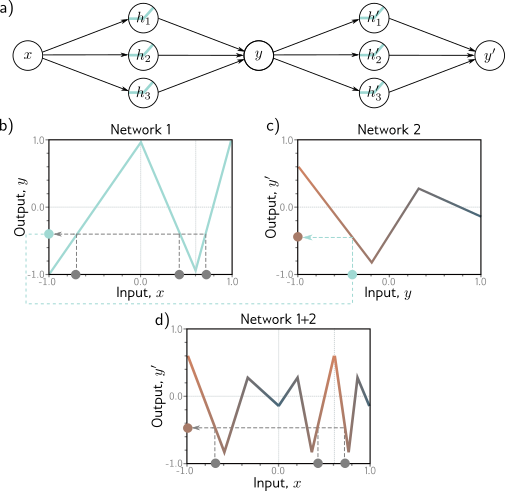
\includegraphics[width=0.7\linewidth]{png/chapter4/DeepConcat.png}
	\caption{结合了各含三个隐藏单元的两个单层网络。a) 第一个网络的输出 y 成为第二个网络的输入。b) 第一个网络通过一个包含三个线性区域的函数,将输入 x(取值范围为 [−1, 1])映射到输出 y(取值范围为 [−1, 1])。这些线性区域的设计目的是让它们的斜率符号交替出现。因此,多个输入 x(以灰色圆圈表示)可以被映射到同一个输出 y(以青色圆圈表示)。c) 第二个网络定义了一个包含三个线性区域的函数,它将输入 y 转换为输出 \(y \prime\)(即将青色圆圈映射到棕色圆圈)。d) 当这两个函数结合后,它们共同作用的结果是:(i) 第一个网络能将三个不同的输入 x 映射到任意一个特定的输出 y,以及 ((ii) 第二个网络以相同的方式处理这些输出;这导致第二个网络在面板 (c) 中定义的函数被重复三次,并根据面板 (b) 中各区域的斜率不同,进行了相应的翻转和缩放处理。}
\end{figure}

\begin{figure}[ht!]
	\centering
	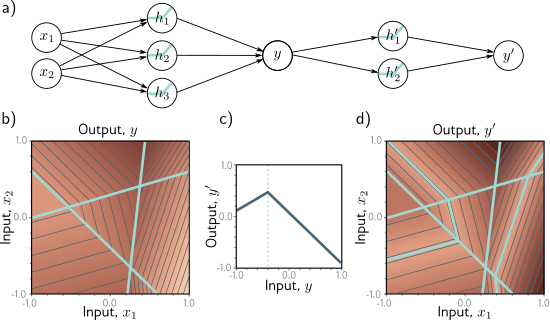
\includegraphics[width=0.7\linewidth]{png/chapter4/DeepTwoLayer2D.png}
	\caption{结合了两个神经网络,输入为二维。a) 第一个网络(源自图 3.8)包含三个隐藏单元,它接收两个输入 x1 和 x2,并输出一个标量 y。这个输出随后被送入一个含有两个隐藏单元的第二网络,生成输出 \(y \prime\)。b) 第一个网络构建的函数包含七个线性区域,其中一个区域保持水平。c) 第二个网络定义了一个在 \(y \in [−1, 1]\) 范围内包含两个线性区域的函数。d) 当这两个网络结合时,第一个网络中的六个非平坦区域每个都被第二网络划分为两个新的区域,总共形成了 13 个线性区域。}
\end{figure}

\begin{figure}[ht!]
	\centering
	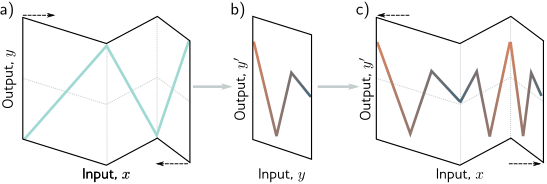
\includegraphics[width=0.7\linewidth]{png/chapter4/DeepFold.png}
	\caption{深层网络用于折叠输入空间。a) 对于图 4.1 中的第一个网络,一种理解方式是它把输入空间折叠,使其叠加在自身之上。b) 第二个网络则在这个已被折叠的空间上施加其功能。c) 最终的输出结果,是在再次展开这些折叠后得到的。}
\end{figure}

\section{从组合网络到深层网络}
上一节我们展示了通过将一个浅层神经网络的输出传递给另一个网络,可以创建复杂的函数。现在我们将说明,这实际上是一个包含两个隐藏层的深层网络的特例。

第一个网络的输出(\(y = \phi_0 + \phi_1h_1 + \phi_2h_2 + \phi_3h_3\))是隐藏单元激活值的线性组合。第二个网络的初始操作(根据方程 4.3,我们计算 \(\theta'_{10}+\theta'_{11}y、\theta'_{20}+\theta'_{21}y 和 \theta'_{30}+\theta'_{31}y\))是对第一个网络输出的线性函数。将一个线性函数应用于另一个线性函数,结果仍然是线性函数。将 y 的表达式代入方程 4.3,可以得到:


\begin{align}
	h'_1 = a[\psi_0 + \theta_{11} \psi_1] = a[\psi_0 + \theta_{11} \phi_0 + \theta_{11} \phi_1 h_1 + \theta_{11} \phi_2 h_2 + \theta_{11} \phi_3 h_3] \notag \\
	h'_2 = a[\psi_0 + \theta_{21} \psi_1] = a[\psi_0 + \theta_{21} \phi_0 + \theta_{21} \phi_1 h_1 + \theta_{21} \phi_2 h_2 + \theta_{21} \phi_3 h_3] \notag \\
	h'_3 = a[\psi_0 + \theta_{31} \psi_1] = a[\psi_0 + \theta_{31} \phi_0 + \theta_{31} \phi_1 h_1 + \theta_{31} \phi_2 h_2 + \theta_{31} \phi_3 h_3] 
\end{align} 


进一步重写为:


\begin{align}
	h'_1 = a[\psi_0 + \psi_{11} h_1 + \psi_{12} h_2 + \psi_{13} h_3] \notag \\
	h'_2 = a[\psi_0 + \psi_{21} h_1 + \psi_{22} h_2 + \psi_{23} h_3] \notag \\
	h'_3 = a[\psi_0 + \psi_{31} h_1 + \psi_{32} h_2 + \psi_{33} h_3], 
\end{align} 


其中 \(\psi_{10} = \theta^\prime_{10} + \theta^\prime_{11} \psi_0, \psi_{11} = \theta^\prime_{11}\psi_1 , \psi_{12} = \theta^\prime_{11}\psi_2\) 等等。这样的结果就是一个拥有两个隐藏层的网络(见图 4.4)。

因此,一个含有两层的网络能够表示那些通过将单层网络的输出传递给另一个网络而创建的函数族。实际上,它能表示一个更广泛的函数族,因为在方程 4.6 中,九个斜率参数 \(\psi_{11}, psi_{21}, ..., psi_{33}\) 可以取任意值。而在方程 4.5 中,这些参数受限于外积 \([\theta^\prime_{11},\theta^\prime_{21},\theta^\prime_{31}]^T[\psi_1, \psi_2, \psi_3]\)。

\section{深度神经网络}
在上一节中,我们展示了将两个浅层网络组合起来可以形成一个有两个隐藏层的特殊深度网络。现在,我们将探讨一个一般情况下的深度网络,它具有两个隐藏层,每层含有三个隐藏单元(见图 4.4)。


\begin{figure}[ht!]
	\centering
	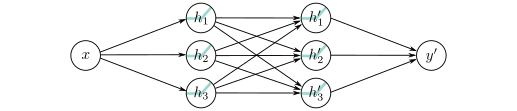
\includegraphics[width=0.7\linewidth]{png/chapter4/DeepTwoLayer.png}
	\caption{ 一个神经网络,它有一个输入、一个输出,并包含两个隐藏层,每层有三个隐藏单元。}
\end{figure}


\begin{figure}[ht!]
	\centering
	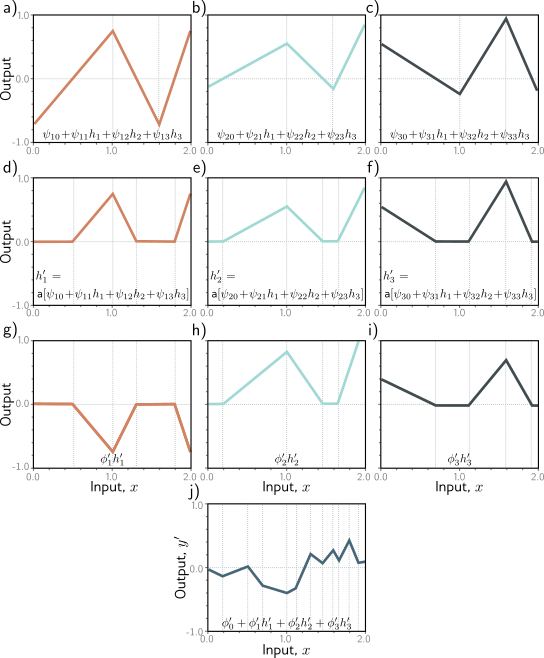
\includegraphics[width=0.7\linewidth]{png/chapter4/DeepBuildUp.png}
	\caption{深层网络的计算过程。a–c) 第二隐藏层接收的输入(即预激活值)是三个分段线性函数,这些函数在相同的位置连接(参见图 3.6)。d–f) ReLU 激活函数将每个分段线性函数的值截断为零。g–i) 接着,这些被截断的函数分别以参数 \(\phi \prime 1、\phi \prime 2 和 \phi \prime 3\) 进行加权处理。j) 最终,这些被截断且加权的函数被相加,并加上一个调节总体高度的偏移 \(\phi \prime 0\)。}
\end{figure}


第一层由以下公式定义:


\begin{align}
	h_1 = a[\theta_{10} + \theta_{11}x] \notag \\
	h_2 = a[\theta_{20} + \theta_{21}x] \notag \\
	h_3 = a[\theta_{30} + \theta_{31}x] 
\end{align} 


接着是第二层:


\begin{align}
	h'_1 = a[\psi_{10} + \psi_{11}h_1 + \psi_{12}h_2 + \psi_{13}h_3] \notag \\
	h'_2 = a[\psi_{20} + \psi_{21}h_1 + \psi_{22}h_2 + \psi_{23}h_3] \notag \\
	h'_3 = a[\psi_{30} + \psi_{31}h_1 + \psi_{32}h_2 + \psi_{33}h_3] 
\end{align} 


以及输出层:

\begin{equation}
y' = \phi_0 + \phi_1h'_1 + \phi_2h'_2 + \phi_3h'_3 
\end{equation}

基于这些方程,我们可以用另一种方式思考网络是如何构建出越来越复杂的函数(见图 4.5):

1. 第一层的三个隐藏单元 \(h_1,h_2,h_3\)通过对输入形成线性函数,然后通过 ReLU 激活函数来计算(参见方程 4.7)。
2. 第二层的激活前状态是通过对这些隐藏单元形成三个新的线性函数来计算的(参见方程 4.8)。此时,我们实际上构建了一个有三个输出的浅层网络,计算了三个具有相同转折点位置的分段线性函数(参见图 3.6)。 
3. 在第二隐藏层,我们对每个函数应用另一个 ReLU 函数 a[⋅] (参见方程 4.8),这会对函数进行裁剪并在每个函数中添加新的转折点。
4. 最终的输出是这些隐藏单元的线性组合(参见方程 4.9)。


总的来说,我们可以从两个角度来理解每一层的作用:一是将输入空间进行“折叠”处理,二是创造新的函数,这些函数经过剪切(形成新的区域)后被重新组合。前者强调了输出函数的依赖关系,但没有突出剪切如何创造新的转折点;而后者则侧重于剪切和转折点的产生,但忽视了输出函数中的依赖性。最终,这两种描述都只能提供对深度神经网络运作方式的部分理解。然而,重要的是不要忘记,这些都只是描述输入 x 与输出 \(y \prime\) 之间关系的方程式。实际上,我们可以将方程式 4.7 到 4.9 结合起来,得到一个更全面的表达式:



\begin{align}
	y' = \phi'_0 &+ \phi'_1 a[\psi_{10} + \psi_{11} a[\theta_{10} + \theta_{11} x]] + \psi_{12} a[\psi_{20} + \psi_{21} a[\theta_{20} + \theta_{21} x]] + \psi_{13} a[\psi_{30} + \psi_{31} a[\theta_{30} + \theta_{31} x]] \notag \\
	&+ \psi'_{2} a[\psi_{20} + \psi_{21} a[\theta_{10} + \theta_{11} x]] + \psi_{22} a[\psi_{20} + \psi_{21} a[\theta_{20} + \theta_{21} x]] + \psi_{23} a[\psi_{30} + \psi_{31} a[\theta_{30} + \theta_{31} x]] \notag \\
	&+ \psi'_{3} a[\psi_{30} + \psi_{31} a[\theta_{10} + \theta_{11} x]] + \psi_{32} a[\psi_{20} + \psi_{21} a[\theta_{20} + \theta_{21} x]] + \psi_{33} a[\psi_{30} + \psi_{31} a[\theta_{30} + \theta_{31} x]] 
\end{align} 


尽管这个表达式确实有些难以理解,但它提供了对深度神经网络内部操作更加全面的视角。

\subsection{超参数}
我们可以将深度网络的结构扩展到不止两个隐藏层;现代的网络可能包含超过一百层,每层拥有数千个隐藏单元。每层隐藏单元的数量称为网络的*宽度*,而隐藏层的数量则称为网络的*深度*。隐藏单元的总数量是衡量网络*容量*的重要指标。

我们用 \(K\) 来代表层数,\(D_1, D_2, \ldots, D_K\) 来表示每层的隐藏单元数量。这些都是*超参数*的典型例子。它们是在学习模型参数(即斜率和截距项)之前确定的量。对于给定的超参数(比如,\(K = 2\) 层,每层有 \(D_k = 3\) 个隐藏单元),模型就定义了一个函数族,而具体的参数则确定了这个族中的特定函数。因此,当我们考虑到超参数时,可以把神经网络看作是一系列函数族,这些函数族将输入与输出相联系。


\section{矩阵表示法}
我们已经了解到深度神经网络是由线性变换和激活函数交替构成的。我们也可以用矩阵表示法来等效地描述方程式 4.7 到 4.9:

\begin{equation}
\begin{bmatrix}
	h_1' \\
	h_2' \\
	h_3'
\end{bmatrix}
= a
\left(
\begin{bmatrix}
	\theta_{10} \\
	\theta_{20} \\
	\theta_{30}
\end{bmatrix}
+
\begin{bmatrix}
	\theta_{11} & \theta_{12} \\
	\theta_{21} & \theta_{22} \\
	\theta_{31} & \theta_{32}
\end{bmatrix}
\begin{bmatrix}
	x_1 \\
	x_2
\end{bmatrix}
\right),
\end{equation}

\begin{equation}
\begin{bmatrix}
	h_1' \\
	h_2' \\
	h_3'
\end{bmatrix}
= a
\left(
\begin{bmatrix}
	\psi_{10} \\
	\psi_{20} \\
	\psi_{30}
\end{bmatrix}
+
\begin{bmatrix}
	\psi_{11} & \psi_{12} & \psi_{13} \\
	\psi_{21} & \psi_{22} & \psi_{23} \\
	\psi_{31} & \psi_{32} & \psi_{33}
\end{bmatrix}
\begin{bmatrix}
	h_1 \\
	h_2 \\
	h_3
\end{bmatrix}
\right),
\end{equation}

以及

\begin{equation}
y' = \phi_0' + 
\begin{bmatrix}
	\phi_1' & \phi_2' & \phi_3'
\end{bmatrix}
\begin{bmatrix}
	h_1' \\
	h_2' \\
	h_3' 
\end{bmatrix},
\end{equation}

或者更简洁地用矩阵表示法表示为:


\begin{align}
	h = a[\theta_0 + \Theta x] \notag \\
	h' = a[\psi_0 + \Psi h] \notag \\
	y' = \phi_0' + \phi'^T h' 
\end{align} 


在每种情况下,函数 \(a[\cdot]\) 都是将激活函数独立地应用于其向量输入的每个元素上。

\subsection{通用公式}
对于层数众多的网络,上述的表示方法可能显得过于复杂。因此,我们从现在开始将第 \(k\) 层的隐藏单元向量记作 \(h_k\),对第 \(k+1\) 层产生影响的偏置(截距)向量记作 \(\beta_k\),以及作用于第 \(k\) 层并影响第 \((k+1)\) 层的权重(斜率)矩阵记作 \(\Omega_k\)。这样,一个包含 \(K\) 层的通用深度网络 \(y = f[x, \phi]\) 可以表示为:


\begin{align}
	h_1 &= a[\beta_0 + \Omega_0 x] \notag \\
	h_2 &= a[\beta_1 + \Omega_1 h_1] \notag \\
	h_3 &= a[\beta_2 + \Omega_2 h_2] \notag \\
	& \vdots \notag \\
	h_K &= a[\beta_{K-1} + \Omega_{K-1}h_{K-1}] \notag \\
	y &= \beta_K + \Omega_K h_K. 
\end{align}

这个模型的参数 \(\phi\) 包括了所有的权重矩阵和偏置向量,表示为 \(\phi = \{ \beta_k, \Omega_k \}^{K}_{k=0}\)。

如果第 \(k\) 层有 \(D_k\) 个隐藏单元,那么偏置向量 \(\beta_{k-1}\) 的维度就是 \(D_k\)。最后一个偏置向量 \(\beta_K\) 的维度是输出的 \(D_0\)。第一个权重矩阵 \(\Omega_0\) 的维度是 \(D_1 \times D_i\),其中 \(D_i\) 是输入的维度。最后一个权重矩阵 \(\Omega_K\) 的维度是 \(D_0 \times D_K\),其余的矩阵 \(\Omega_k\) 的维度是 \(D_{k+1} \times D_k\)(参见图 4.6)。

\begin{figure}[ht!]
	\centering
	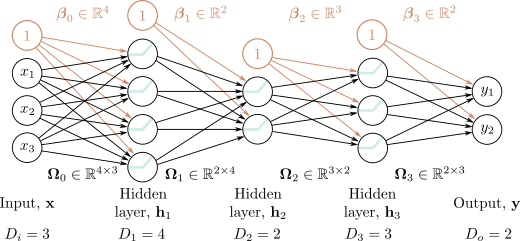
\includegraphics[width=0.7\linewidth]{png/chapter4/DeepKLayer.png}
	\caption{图 4.6: 描述一个具有 Di = 3维输入 x、Do = 2维输出 y 以及 K = 3个隐藏层 h1、h2、h3 的网络的矩阵表示法,这些隐藏层的维度分别是 D1 = 4、D2 = 2 和 D3 = 3。权重以矩阵 \(\Omega k\) 的形式存储,通过与前一层的激活值相乘来为下一层生成预激活值。例如,\(\Omega_1\) 是一个 2 × 4 的矩阵,用于计算从第一层的激活值到第二层的预激活值。这个矩阵作用于第一层的四个隐藏单元,并为第二层的两个隐藏单元生成输入。偏置则以向量 \(\beta_k\) 的形式存储,其维度与其输入的层相对应。比如,偏置向量 \(\beta_2\) 长度为三,因为 h3 层包含三个隐藏单元。}
\end{figure}

我们也可以将整个网络等效地表示为一个单一函数:


\begin{equation}
y = \beta_K + \Omega_K [\beta_{K-1} + \Omega_{K-1} [ \ldots a[\beta_2 + \Omega_2 [a[\beta_1 + \Omega_1 [a[\beta_0 + \Omega_0 x]] \ldots ]]. 
\end{equation}

\section{浅层网络与深层网络的比较}
第 3 章讨论了单隐藏层的浅层网络,而本章我们讨论了多隐藏层的深层网络。现在,我们来比较这两种模型。

\subsection{逼近不同函数的能力}
在第 3.2 节,我们提出了一个观点:具备足够容量(隐藏单元)的浅层神经网络能够极其接近地模拟任何连续函数。本章我们了解到,一个包含两个隐藏层的深层网络能够实现两个浅层网络的功能组合。如果其中一个网络执行恒等函数,那么这个深层网络就等同于一个浅层网络。因此,它也能在拥有足够容量的情况下非常接近地逼近任何连续函数。

\subsection{每个参数产生的线性区域数量}
一个有一个输入、一个输出和 \(D > 2\) 个隐藏单元的浅层网络能够创造最多 \(D + 1\) 个线性区域,由 \(3D + 1\) 个参数定义。相比之下,一个有一个输入、一个输出和 \(K\) 层 \(D > 2\) 个隐藏单元的深层网络能够使用 \(3D + 1 + (K - 1)D(D + 1)\) 个参数创造最多 \((D + 1)^K\) 个线性区域的函数。

图 4.7a 展示了对于将标量输入 \(x\) 映射到标量输出 \(y\) 的网络,最大线性区域数量随参数数量增加而增加的趋势。深层神经网络在固定参数预算下可以创造出更复杂的函数。当输入维度 \(D_i\) 增加时,这种效果更加显著(参见图 4.7b),尽管计算最大区域数量的方法更加复杂。

\begin{figure}[ht!]
	\centering
	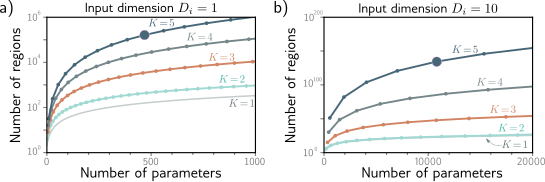
\includegraphics[width=0.7\linewidth]{png/chapter4/DeepParams.png}
	\caption{图 4.7: 随着网络深度的增加,神经网络能够产生的线性区域数量急剧增加。a) 输入为 Di = 1 的网络。每条曲线代表在不同隐藏层 K 数量下,变化每层隐藏单元 D 数量的情况。在相同参数限制(水平位置)下,较深的网络能比较浅的网络产生更多线性区域。例如,一个 K = 5 层、每层 D = 10 隐藏单元的网络有 471 个参数(突出显示的点),可以产生 161,051 个区域。b) 输入为 Di = 10 的网络。曲线上的每个点代表增加了十个隐藏单元。在这种情况下,一个 K = 5 层、每层 D = 50 隐藏单元的模型拥有 10,801 个参数(突出显示的点),能创建超过 $10^134$ 个线性区域。}
\end{figure}

尽管这听起来很吸引人,但函数的灵活性仍然受到参数数量的限制。深度网络能够创建大量的线性区域,但这些区域中存在着复杂的依赖性和对称性。我们在之前讨论过深层网络如何通过“折叠”输入空间来实现这一点(参见图 4.3)。因此,除非我们希望逼近的现实世界函数中存在相似的对称性,或者我们有理由相信输入到输出的映射真的涉及到简单函数的组合,否则更多的区域数量并不一定是一个优势。

\subsection{深度效率}
深层和浅层网络都能模拟任意函数,但某些函数使用深层网络进行逼近会更有效率。事实上,已经发现某些函数需要浅层网络有指数级更多的隐藏单元才能与深层网络实现同等水平的逼近。这种现象被称为神经网络的“深度效率”。虽然这听起来很有吸引力,但目前尚不清楚我们想要逼近的真实世界函数是否符合这种特性。

\subsection{大型结构化输入}
我们讨论了每一层的每个元素都与下一层的每个元素相连的完全连接网络。但这种网络对于像图像这样的大型结构化输入来说并不实际,因为输入可能包含大约 $10^6$ 个像素。参数数量会非常庞大,而且我们希望图像的不同部分以类似的方式进行处理;没有必要在图像的每个可能位置都独立学习识别同一对象。

解决方案是并行处理图像的局部区域,然后逐步整合来自更大区域的信息。这种由局部到全局的处理方式在没有多层结构的情况下很难实现(参见第 10 章)。

\subsection{训练和泛化}
深层网络相比于浅层网络的另一个潜在优势是它们更容易训练;通常训练中等深度的网络比浅层网络要容易(参见图 20.2)。这可能是因为过度参数化的深层模型存在许多大致相同且易于找到的解决方案。然而,随着隐藏层的增加,训练又变得更加困难,尽管已经发展了许多缓解这一问题的方法(参见第 11 章)。

深度神经网络在泛化到新数据方面似乎也比浅层网络表现更佳。在实际应用中,大多数任务的最佳结果是通过使用数十甚至数百层的网络实现的。这两种现象都尚未被充分理解,我们将在第 20 章中进一步探讨这些主题。
\section{总结}
本章首先探讨了组合两个浅层网络时所发生的情况。我们认为,第一个网络对输入空间进行了“折叠”,随后第二个网络应用了一个分段线性函数。在输入空间被折叠到其自身时,第二个网络的效果得到了复制。

接着,我们证明了这种浅层网络组合实际上是具有两个隐藏层的深层网络的一种特例。我们解释了每一层中的 ReLU 函数如何在多个位置剪切输入函数,并在输出函数中创建更多的“关节”。我们引入了超参数的概念,对于我们目前讨论的网络而言,它包括了隐藏层的数量和每层中隐藏单元的数量。

最后,我们对浅层和深层网络进行了比较。我们发现:(i) 给定足够容量,两种网络都能逼近任何函数;(ii) 相比之下,深层网络每个参数能产生更多的线性区域;(iii) 某些函数可以通过深层网络更有效率地逼近;(iv) 像图像这样的大型结构化输入更适合通过多阶段处理;(v) 实践中,大多数任务使用多层的深层网络能达到最佳效果。

了解了深层和浅层网络模型后,我们接下来将关注它们的训练过程。在下一章,我们将讨论损失函数,它对于任何给定的参数值 \(\phi\),提供了一个指标,显示模型输出与训练数据集中的真实预测之间的差异。在第 6 章和第 7 章中,我们将深入训练过程本身,探索如何寻找使损失最小化的参数值。


\section{Notes}
\textbf{深度学习}:长期以来人们已经理解,通过组合浅层神经网络或发展具有多个隐藏层的网络,可以构建更复杂的函数。事实上,“深度学习”这个术语最早由 Dechter 在 1986 年使用。然而,由于实际问题,人们对此的兴趣有限;无法很好地训练这些网络。深度学习的现代时代是由 Krizhevsky 等人在 2012 年报告的图像分类方面的惊人改进所启动的。这一突破性进展可以说是由四个因素的汇聚造成的:更大的训练数据集、训练时更强大的处理能力、使用 ReLU 激活函数和使用随机梯度下降(见第 6 章)。LeCun 等人在 2015 年提供了现代深度学习早期进展的概览。

\textbf{线性区域数量}:对于使用总共 \(D\) 个隐藏单元和 ReLU 激活的深度网络,区域数量的上限是 \(2^D\)(Montufar 等人,2014)。同样的作者展示了一个具有 \(D_i\) 维输入和 \(K\) 层、每层包含 \(D \geq D_i\) 个隐藏单元的深度 ReLU 网络,具有 \(O\left(\left(\frac{D}{D_i}\right)^{(K-1)D_i}D D_i\right)\) 个线性区域。Montufar(2017)、Arora 等人(2016)和 Serra 等人(2018)都提供了考虑到每层有不同数量隐藏单元的可能性的更紧密的上限。Serra 等人(2018)提供了一个计算神经网络中线性区域数量的算法,尽管它只适用于非常小的网络。

如果 \(K\) 层中的每层隐藏单元数量 \(D\) 相同,并且 \(D\) 是输入维度 \(D_i\) 的整数倍,则最大线性区域数量 \(N_r\) 可以精确计算,为:

\begin{equation}
N_r = \left( \frac{D}{D_i} + 1 \right)^{D_i(K-1)} \cdot \sum_{j=0}^{D_i} \binom{D}{j} 
\end{equation}

这个表达式中的第一项对应于网络的前 \(K - 1\) 层,可以被认为是反复折叠输入空间。然而,我们现在需要将 \(\frac{D}{D_i}\) 个

隐藏单元分配给每个输入维度以创建这些折叠。这个方程中的最后一项(二项式系数之和)是浅层网络可以创建的区域数量,归因于最后一层。更多信息,请参考 Montufar 等人(2014)、Pascanu 等人(2013)和 Montufar(2017)。

\textbf{通用逼近定理}:我们在 4.5.1 节中讨论了一个观点,即如果深度网络的各层包含足够多的隐藏单元,那么宽度版本的通用逼近定理将适用。这意味着存在一种网络结构,它能够在 \(R^{D_i}\) 的一个紧凑子集上,以任意精度逼近任何给定的连续函数。Lu et al. (2017) 证实,只要层数足够,每层至少包含 \(D_i + 4\) 个隐藏单元的带有 ReLU 激活函数的网络,能够以任意精度逼近任何指定的 \(D_i\) 维勒贝格(Lebesgue)可积函数。这被称作通用逼近定理的\textbf{深度版本}。

\textbf{深度效率}:近期研究显示,某些函数可以被深度网络实现,但无法被容量上限呈指数级增长的浅层网络所表达。换言之,浅层网络要准确描述这些函数,需要指数级增加其单元数量。这种现象被称为神经网络的\textbf{深度效率}。

Telgarsky (2016) 指出,对于任意整数 \(k\),可以构建一个具有单一输入、单一输出,并且包含 \(O[k^3]\) 层恒定宽度的网络,这样的网络不能用少于 \(2^k\) 宽度的 \(O[k]\) 层来实现。更令人惊讶的是,Eldan \& Shamir (2016) 发现,当涉及到多变量输入时,某些三层网络无法由任何两层网络实现,前提是两层网络的容量低于输入维度的亚指数级。Cohen et al. (2016)、Safran \& Shamir (2017. 和 Poggio et al. (2017) 同样展示了深层网络能够有效逼近的函数,而这些函数对于浅层网络却难以做到。Liang \& Srikant (2016) 则表明,在一定的逼近误差上限条件下,对于包括单变量函数在内的广泛函数类别,浅层网络需要远比深层网络多的指数级隐藏单元。

\textbf{宽度效率}:Lu et al. (2017) 探讨了这样一个问题:是否存在宽而浅的网络(即,隐藏单元众多的浅层网络),而这些网络却无法通过深度不显著增加的窄网络来实现。他们发现,确实存在一类宽而浅的网络,只有通过深度为多项式级别的窄网络才能表达。这被称为神经网络的\textit{宽度效率}。相对于深度的指数级下界限制,宽度的多项式级下界限制显得更为宽松,这表明在网络设计中,深度比宽度更为重要。Vardi et al. (2022) 进一步证明,对于带有 ReLU 激活函数的网络,减小宽度的代价仅是网络深度的线性增加。

\section{Problems}
\textbf{问题 4.1} 考虑组合图 4.8 中的两个神经网络。请绘制一张图,展示当输入 \(x\) 在 [-1,1] 范围内变化时,输出 \(y'\) 的变化关系。


\begin{figure}[ht!]
	\centering
	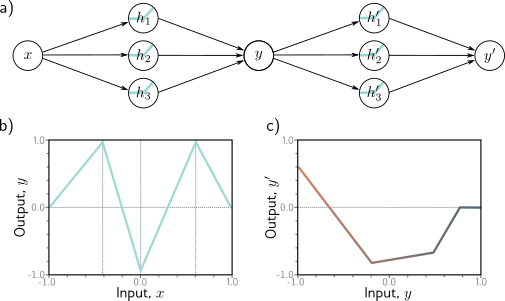
\includegraphics[width=0.7\linewidth]{png/chapter4/DeepConcatQuestion.png}
	\caption{图 4.8: 针对问题 4.1,展示了两个网络的组合。a) 第一个网络的输出 y 转化为第二个网络的输入。b) 第一个网络在输出值 \(y \in [−1, 1]\) 的范围内计算该函数。c) 第二个网络则在输入范围 \(y \in [−1, 1]\) 内计算该函数。}
\end{figure}

\textbf{问题 4.2} 请确定图 4.6 中的四个超参数。

\textbf{问题 4.3} 利用 ReLU(修正线性单元)函数的非负同质性质(见问题 3.5),证明以下等式:
\begin{equation}
ReLU[\beta_1 + \lambda_1 \cdot \Omega_1 ReLU[\beta_0 + \lambda_0 \cdot \Omega_0 x]] = \lambda_0\lambda_1 · ReLU[\frac{1}{\lambda_0\lambda_1} \beta_1 + \Omega_1 ReLU[\frac{1}{\lambda_0} \beta_0 + \Omega_0 x]]  
\end{equation}

其中 \(\lambda_0\) 和 \(\lambda_1\) 是非负数值标量。由此可见,只要同时调整偏置,并在网络末端重新应用这些缩放因子,就可以任意缩放权重矩阵。

\textbf{问题 4.4} 编写一个深度神经网络的方程,该网络有 \(D_i = 5\) 个输入、\(D_o = 4\) 个输出,并且有三个隐藏层,其大小分别为 \(D_1 = 20\)、\(D_2 = 10\) 和 \(D_3 = 7\)。使用方程式 4.15 和 4.16 的形式表示。每个权重矩阵(Weight Matrix)\(\Omega\) 和偏置向量(Bias Vector)\(\beta\) 的大小分别是多少?

\textbf{问题 4.5} 考虑一个深度神经网络,它有 \(D_i = 5\) 个输入、\(D_o = 1\) 个输出,以及 \(K = 20\) 个隐藏层,每层含有 \(D = 30\) 个隐藏单元。请问这个网络的深度和宽度分别是多少?

\textbf{问题 4.6} 考虑一个网络,它有 \(D_i = 1\) 个输入、\(D_o = 1\) 个输出,并且有 \(K = 10\) 层,每层包含 \(D = 10\) 个隐藏单元。如果我们增加一层深度或增加每层的单元数量,哪种情况下权重的数量会增加更多?请给出你的理由。

\textbf{问题 4.7} 为方程 3.1 中的浅层神经网络选择参数 \(\phi = {\phi_0, \phi_1, \phi_2, \phi_3, \theta_{10}, \theta_{11}, \theta_{20}, \theta_{21}, \theta_{30}, \theta_{31}}\) 的值,使得该网络在有限范围 \(x \in [a, b]\) 上定义一个恒等函数。

\textbf{问题 4.8}* 图 4.9 展示了一个浅层网络(如图 3.3 所示)中三个隐藏单元的激活情况。隐藏单元的斜率分别为 1.0, 1.0 和 -1.0,隐藏单元的“关节”位置分别在 1/6, 2/6 和 4/6。找出 \(\phi_0, \phi_1, \phi_2\) 和 \(\phi_3\) 的值,使得隐藏单元激活的组合为 \(\phi_0 + \phi_1 h_1 + \phi_2 h_2 + \phi_3 h_3\),以创建一个具有四个线性区域的函数,这些区域的输出值在零和一之间摆动。最左边区域的斜率应该是正的,下一个是负的,依此类推。如果我们将这个网络与自身组合,将会创建多少个线性区域?如果我们将其与自身组合 \(K\) 次,将会创建多少个?

\begin{figure}[ht!]
	\centering
	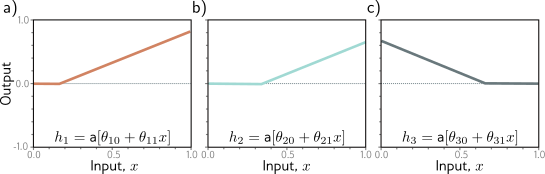
\includegraphics[width=0.7\linewidth]{png/chapter4/DeepProbZeroCross.png}
	\caption{图 4.9: 针对问题 4.8 的隐藏单元激活情况。a) 第一个隐藏单元在 x = 1/6 的位置形成一个拐点,其激活区域的斜率为正一。b) 第二个隐藏单元在 x = 2/6 的位置形成一个拐点,其激活区域的斜率同样为正一。c) 第三个隐藏单元在 x = 4/6 的位置形成一个拐点,但其激活区域的斜率为负一。}
\end{figure}


\textbf{问题 4.9}* 继续问题 4.8,使用一个有两个隐藏单元的浅层网络,能否创建一个具有三个线性区域的函数,其输出值在零和一之间来回摆动?使用一个有四个隐藏单元的浅层网络,能否创建一个以同样方式摆动的具有五个线性区域的函数?

\textbf{问题 4.10} 考虑一个深度神经网络,它有一个输入、一个输出,以及 \(K\) 个隐藏层,每层包含 \(D\) 个隐藏单元。展示这个网络总共有 \(3D + 1 + (K - 1)D(D + 1)\) 个参数。

\textbf{问题 4.11}* 考虑两个将标量输入 \(x\) 映射到标量输出 \(y\) 的神经网络。第一个网络是浅层的,有 \(D = 95\) 个隐藏单元。第二个是深层的,有 \(K = 10\) 层,每层包含 \(D = 5\) 个隐藏单元。每个网络有多少参数?每个网络可以制造多少个线性区域?哪个运行得更快?



\chapter{损失函数}

前三章分别介绍了线性回归、浅层神经网络和深度神经网络。这些都属于函数家族,能够实现从输入到输出的映射,其具体的函数取决于模型参数 \(\phi\)。在训练这些模型时,我们的目标是找到能够为特定任务提供最优输入输出映射的参数。本章将详细阐述“最优映射”的含义。

要定义“最优映射”,首先需要一组训练数据集 \(\{x_i, y_i\}\),即输入和输出的配对。损失函数(Loss Function)\(L[\phi]\) 能够返回一个数值,这个数值描述了模型预测 \(f(x_i, \phi)\) 与其对应的真实输出 \(y_i\) 之间的不匹配程度。在训练过程中,我们追求的是能最小化损失的参数值 \(\phi\),以使训练输入尽可能准确地映射到输出。例如,在第2章中,我们见到了一种损失函数——最小平方损失函数,适用于目标是实数 \(y \in \mathbb{R}\) 的单变量回归问题。该函数通过计算模型预测 \(f(x_i, \phi)\) 与真实值 \(y_i\) 之间差异的平方和来进行计算。

本章还提出了一个框架,不仅证明了在实值输出场景下选择最小平方准则的适用性,还指导我们为其他类型的预测问题构建损失函数。我们将讨论包括二元分类(其中预测结果 \(y \in \{0, 1\}\) 属于两个类别中的一个)和多类别分类(预测结果 \(y \in \{1, 2, \ldots, K\}\) 属于 \(K\) 个类别中的一个)在内的多种情形。在接下来的两章中,我们将探讨模型训练的过程,目标是找到能最小化这些损失函数的参数值。

\section{最大似然}
在本节中,我们将介绍构建损失函数的具体方法。设想一个计算输入 \(x\) 到输出的模型 \(f(x, \phi)\),其中 \(\phi\) 是模型的参数。之前,我们认为模型直接输出预测结果 \(y\)。现在,我们改变思路,将模型视为计算给定输入 \(x\) 时,可能的输出 \(y\) 的条件概率分布 \(Pr(y|x)\)。这种损失函数的设计目的是使得每个训练输出 \(y_i\) 在由对应输入 \(x_i\) 计算得到的分布 \(Pr(y_i|x_i)\) 中具有较高的概率(见图 5.1)。

\begin{figure}[ht!]
	\centering
	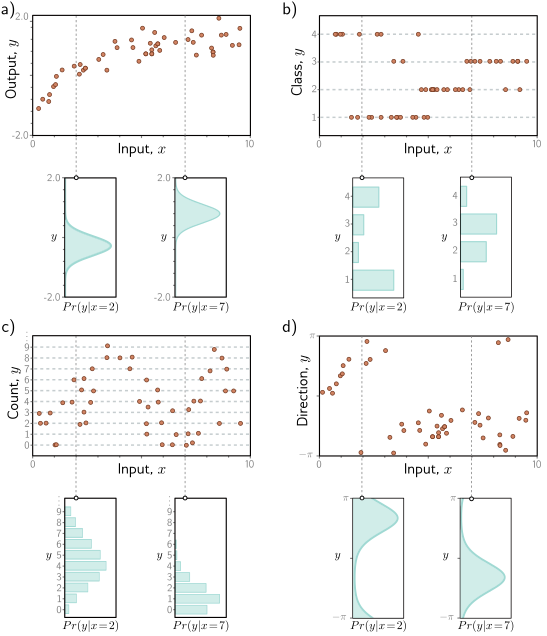
\includegraphics[width=0.7\linewidth]{png/chapter5/LossDataTypes.png}
	\caption{a) 回归任务中,目标是基于训练数据 {xi,yi}(橙色点)从输入 x 预测出一个实数输出 y。对于每个输入值 x,机器学习模型预测输出 \(y \in R\) 的分布 P(y|x)(青色曲线展示了 x = 2.0 和 x = 7.0 时的分布)。损失函数的目的是使根据相应输入 xi 预测出的分布最大化观测到的训练输出 yi 的概率。b) 在分类任务中,为预测离散类别 \(y \in {1, 2, 3, 4}\),我们采用离散概率分布,模型因此针对 xi 的每个值预测 yi 的四个可能值的概率分布直方图。c) 在预测计数 \(y \in {0, 1, 2, ...}\) 和 d) 预测方向 \(y \in (−\pi, \pi]\) 的任务中,我们分别采用定义在正整数集和圆周域上的分布。}
\end{figure}


\subsection{计算输出的分布}
这引出了一个问题:模型 \(f(x, \phi)\) 如何转化为计算概率分布的形式。答案很简单。首先,我们需要选定一个定义在输出域 \(Y\) 上的参数化概率分布 \(Pr(y|\theta)\)。接着,我们利用神经网络来计算该分布的一个或多个参数 \(\theta\)。

例如,假设预测域是实数集,即 \(y \in \mathbb{R}\)。在这种情况下,我们可能选择单变量正态分布,它在 \(\mathbb{R}\) 上有定义。该分布由均值 \(\mu\) 和方差 \(\sigma^2\) 所决定,因此 \(\theta = \{\mu, \sigma^2\}\)。机器学习模型可以用来预测均值 \(\mu\),而方差 \(\sigma^2\) 则可以视为一个待定的常数。
\subsection{最大似然准则}
模型现在针对每个训练输入 \(x_i\) 计算不同的分布参数 \(\theta_i = f(x_i, \phi)\)。我们的目标是使每个训练输出 \(y_i\) 在其相应的分布 \(Pr(y_i|\theta_i)\) 下具有较高概率。因此,我们选择模型参数 \(\phi\),以最大化所有 \(I\) 个训练样本的联合概率:

\begin{align}
	\hat{\phi} &= argmax_{\phi} \left[ \prod_{i=1}^{I} Pr(y_i|x_i) \right] \notag \\
	&= argmax_{\phi} \left[ \prod_{i=1}^{I} Pr(y_i|\theta_i) \right] \notag \\
	&= argmax_{\phi} \left[ \prod_{i=1}^{I} Pr(y_i|f(x_i, \phi)) \right]  
\end{align} 


这个联合概率项反映的是参数的似然(Likelihood),因此方程 5.1 称为最大似然准则(Maximum Likelihood Criterion)[1]。

这里我们基于两个假设。首先,我们假设所有数据点的输出 \(y_i\) 都服从相同的概率分布,即数据是同分布的。其次,我们认为给定输入的输出的条件分布 \(Pr(y_i|x_i)\) 是相互独立的,因此整个训练数据集的似然可以表示为:

\begin{equation}
Pr(y_1, y_2, \ldots , y_I|x_1, x_2, \ldots , x_I) = \prod_{i=1}^{I} Pr(y_i|x_i) 
\end{equation}

换言之,我们假定数据是独立同分布(i.i.d.)的。

\begin{figure}[ht!]
	\centering
	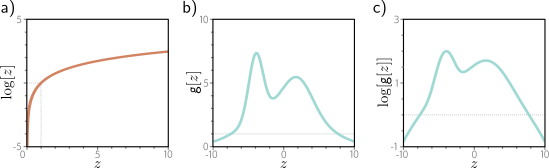
\includegraphics[width=0.7\linewidth]{png/chapter5/LossLog.png}
	\caption{对数变换。a) 对数函数是单调递增的,即若 \(z > z \prime \),则 \(log z > log z \prime\)。因此,任何函数 g(z) 的最大值位置与 log g(z) 的最大值位置相同。b) 函数 g(z)。c) 该函数的对数 log g(z)。g(z) 上所有正斜率的位置在经过对数变换后依然保持正斜率,负斜率的位置同样保持负斜率。最大值位置不变。}
\end{figure}

\subsection{最大化对数似然}
尽管最大似然准则(方程 5.1)理论上有效,但在实际应用中并不方便。每个项 \(Pr(y_i|f(x_i, \phi))\) 的值可能很小,导致这些项的乘积极小,难以用有限精度算法精确表示。幸运的是,我们可以通过最大化似然的对数来解决这个问题:


\begin{align}
	\hat{\phi} &= argmax_{\phi} \left[ \prod_{i=1}^{I} Pr(y_i|f(x_i, \phi)) \right] \notag \\
	&= argmax_{\phi} \left[ \log \prod_{i=1}^{I} Pr(y_i|f(x_i, \phi)) \right] \notag \\
	&= argmax_{\phi} \left[ \sum_{i=1}^{I} \log Pr(y_i|f(x_i, \phi)) \right] 
\end{align} 


由于对数是单调递增函数,对数似然准则与原始最大似然准则在数学上是等价的。这意味着,提高对数似然准则的同时,也就提高了最大似然准则。因此,两种准则的最大值位置是相同的,最优的模型参数 \(\hat{\phi}\) 在两种情况下都是一致的。同时,对数似然准则通过求和而非乘积,避免了精度问题。
\subsection{最小化负对数似然}

通常,模型拟合问题是以最小化损失的方式来定义的。为了将最大对数似然准则转换为一个最小化问题,我们通过乘以负一得到负对数似然准则:


\begin{align}
	\hat{\phi} &= argmin_{\phi} \left[ - \sum_{i=1}^{I} \log Pr(y_i|f(x_i, \phi)) \right] \notag \\
	&= argmin_{\phi} [ L[\phi] ] 
\end{align}

这就构成了最终的损失函数 \(L[\phi]\)。

\subsection{推断}

如今,网络不再直接预测输出 \(y\),而是确定了一个关于 \(y\) 的概率分布。在进行推断时,我们一般需要一个具体的估计值而不是整个分布,因此我们选择分布的最大值作为预测:

\begin{equation}
	\hat{y} = argmax_y [Pr(y|f(x, \phi))]  
\end{equation}


我们通常可以根据模型预测的分布参数 \(\theta\) 来确定这个估计值。例如,在单变量正态分布中,最大值出现在均值 \(\mu\) 处。


\section{构建损失函数的步骤}

根据最大似然方法,针对训练数据 \(\{x_i, y_i\}\) 构建损失函数的步骤如下:

1. 选定一个适合预测结果 \(y\) 的概率分布 \(Pr(y|\theta)\),并确定其分布参数 \(\theta\)。
2. 设定机器学习模型 \(f(x, \phi)\) 来预测这些参数中的一个或多个,即 \(\theta = f(x, \phi)\),\(Pr(y|\theta) = Pr(y|f(x, \phi))\)。
3. 为训练模型,寻找最小化负对数似然损失函数的模型参数 \(\phi\):

\begin{equation}
	\hat{\phi} = argmin_{\phi} [ L[\phi] ] = argmin_{\phi} \left[ - \sum_{i=1}^{I} \log Pr(y_i|f(x_i, \phi)) \right] 
\end{equation}


4. 对于新的测试样例 \(x\),返回完整分布 \(Pr(y|f(x, \phi))\) 或此分布的最大值。

本章其余部分主要讨论如何使用这种方法为常见的预测类型构建损失函数。

\begin{figure}[ht!]
	\centering
	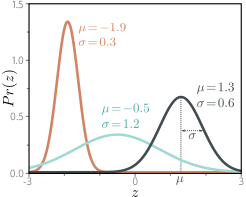
\includegraphics[width=0.7\linewidth]{png/chapter5/LossNorm.png}
	\caption{单变量正态分布(也被称为高斯分布)是在实数轴 \(z \in R\) 上定义的,其主要由两个参数 \(\mu\) 和 \(\sigma_2\) 决定。其中,均值 \(\mu\) 决定了分布的峰值位置,而方差 \(\sigma_2\) 的标准差(即方差的正平方根)则决定了分布的宽度。因为整个概率密度的总和为一,所以当方差减小,分布变得更加集中时,其峰值也相应地变得更高。}
\end{figure}

\section{示例 1:单变量回归}

首先考虑单变量回归模型。这里的目标是用带有参数 \(\phi\) 的模型 \(f(x, \phi)\),从输入 \(x\) 预测单一实数输出 \(y \in \mathbb{R}\)。遵循上述步骤,我们为输出域 \(y\) 选择一个概率分布。我们选用单变量正态分布(见图 5.3),它定义在 \(y \in \mathbb{R}\) 上。该分布有两个参数(均值 \(\mu\) 和方差 \(\sigma^2\)),并具有概率密度函数:

\begin{equation}
	Pr(y|\mu, \sigma^2) = \frac{1}{\sqrt{2\pi\sigma^2}} \exp \left[ -\frac{(y - \mu)^2}{2\sigma^2} \right] 
\end{equation}

接着,我们让机器学习模型 \(f(x, \phi)\) 计算这个分布的一个或多个参数。在这里,我们只计算均值 \(\mu = f(x, \phi)\):

\begin{equation}
Pr(y|f(x, \phi), \sigma^2) = \frac{1}{\sqrt{2\pi\sigma^2}} \exp \left[ -\frac{(y - f(x, \phi))^2}{2\sigma^2} \right] 
\end{equation}
我们的目标是找到使训练数据 \(\{x_i, y_i\}\) 在此分布下尽可能概率最高的参数 \(\phi\)(参见图 5.4)。为此,我们选择了基于负对数似然的损失函数 \(L[\phi]\):

\begin{align}
	L[\phi] &= - \sum_{i=1}^{I} \log \left[ Pr(y_i|f(x_i, \phi), \sigma^2) \right] \notag \\
	&= - \sum_{i=1}^{I} \log \left[ \frac{1}{\sqrt{2\pi\sigma^2}} \exp \left[ -\frac{(y_i - f(x_i, \phi))^2}{2\sigma^2} \right] \right] 
\end{align}

在训练模型时,我们的目标是找到最小化这一损失的参数 \(\hat{\phi}\)。

\subsection{最小平方损失函数}

我们对损失函数进行一系列代数操作,目的是寻找:


\begin{align}
	\hat{\phi} &= argmin_{\phi} \left[ -\sum_{i=1}^{I} \log \left[ \frac{1}{\sqrt{2\pi\sigma^2}} \exp \left[ -\frac{(y_i - f(x_i, \phi))^2}{2\sigma^2} \right] \right] \right] \notag \\
	&= argmin_{\phi} \left[ -\sum_{i=1}^{I} ( \log \frac{1}{\sqrt{2\pi\sigma^2}} - \frac{(y_i - f(x_i, \phi))^2}{2\sigma^2} ) \right] \notag \\
	&= argmin_{\phi} \left[ \sum_{i=1}^{I} \frac{(y_i - f(x_i, \phi))^2}{2\sigma^2} \right] 
\end{align}

在这里,我们去除了与 \(\phi\) 无关的项,并忽略了常数缩放因子,因为它不影响最小值的位置。

通过这些操作,我们得到了最小平方损失函数,这是我们在第2章讨论线性回归时首次提出的:

\begin{equation}
L[\phi] = \sum_{i=1}^{I} (y_i - f(x_i, \phi))^2 
\end{equation}
最小平方损失函数的自然来源于两个假设:预测误差(i)是独立的,并且(ii)遵循均值为 \(\mu = f(x_i, \phi)\) 的正态分布(参见图 5.4)。


\subsection{推断}

网络现在不直接预测 \(y\),而是预测 \(y\) 的正态分布均值 \(\mu = f(x, \phi)\)。在进行推断时,我们通常寻求一个最佳的单点估计,因此我们选择预测分布的最大值:

\begin{equation}
\hat{y} = argmax_y [Pr(y|f(x, \phi))] 
\end{equation}


在单变量正态分布中,最大值位置由均值参数 \(\mu\) 决定(参见图 5.3)。这正是模型所计算的,因此 \(\hat{y} = f(x, \phi)\)。
\subsection{估计方差}

在制定最小平方损失函数时,我们假定网络预测了正态分布的均值。有趣的是,方程 5.11 中的最终表达式并不依赖于方差 \(\sigma^2\)。但我们可以将 \(\sigma^2\) 视为模型的参数之一,并对模型参数 \(\phi\) 和分布的方差 \(\sigma^2\) 一起最小化方程 5.9:


\begin{equation}
\hat{\phi}, \hat{\sigma}^2 = \arg\min_{\phi,\sigma^2} \left[ -\sum_{i=1}^I \log \left[ \frac{1}{\sqrt{2\pi\sigma^2}} \exp \left( -\frac{(y_i - f(x_i; \phi))^2}{2\sigma^2} \right) \right] \right] 
\end{equation}


在推断阶段,模型从输入中预测均值 \(\mu = f[x, \hat{\phi}]\),同时我们在训练过程中得到了方差 \(\hat{\sigma}^2\) 的估计。均值是最优预测,而方差反映了预测的不确定性。

\begin{figure}[ht!]
	\centering
	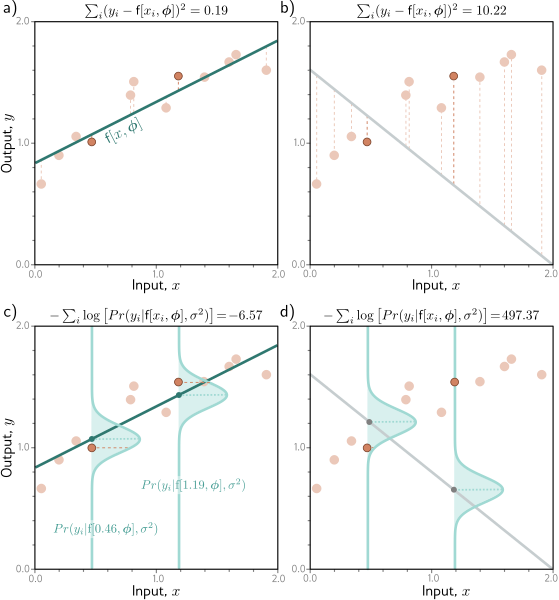
\includegraphics[width=0.7\linewidth]{png/chapter5/LossNormalRegression.png}
	\caption{最小二乘法与正态分布最大似然损失的等效性。a) 参照图 2.2 中的线性模型。最小二乘法通过最小化模型预测值 \(f[xi,\phi]\)(绿线)与真实输出值 yi(橙色点)之间差异(虚线表示)的平方和来进行优化。在此例中,模型拟合非常准确,因此这些差异非常小(比如,对于被特别标出的两个点)。b) 当参数设置不当时,模型拟合效果较差,导致平方差异显著增加。c) 最小二乘法的原理是假设模型预测的是输出值的正态分布的平均值,并且我们通过最大化概率来优化它。在第一种情况下,由于模型拟合得很好,所以数据的概率 Pr(yi|xi)(水平橙色虚线)较高(相应的负对数概率较小)。d) 在第二种情况下,由于模型拟合效果差,因此概率较低,负对数概率较高。}
\end{figure}


\subsection{异方差回归}

先前的模型假定数据方差是固定的,但这可能不太现实。当模型的不确定性随输入数据变化时,我们称之为异方差(与同方差相对,后者不确定性是固定的)。

一种处理这种情况的简单方法是训练一个神经网络 \(f(x, \phi)\) 来同时计算均值和方差。举个例子,考虑一个输出两个值的浅层网络,其中第一个输出 \(f_1(x, \phi)\) 预测均值,第二个输出 \(f_2(x, \phi)\) 预测方差。

为了确保计算的方差始终为正,我们需要对网络的第二个输出应用一个能映射到正数的函数。一个好的选择是使用平方函数,得到:


\begin{align}
	\mu = f_1(x, \phi)  \notag \\
	\sigma^2 = f_2(x, \phi)^2  
\end{align}

这样就得到了以下损失函数:

\begin{equation}
	\hat{\phi} = argmin_{\phi} \left[ -\sum_{i=1}^{I} \log \left[ \frac{1}{\sqrt{2\pi f_2(x_i, \phi)^2}} \exp \left[ -\frac{(y_i - f_1(x_i, \phi))^2}{2f_2(x_i, \phi)^2} \right] \right] \right] 
\end{equation}

图 5.5 对比了同方差和异方差模型。

\section{示例 2:二元分类}

在二元分类任务中,我们的目标是根据数据 \(x\) 将其划分为两个离散类别之一 \(y \in \{0, 1\}\)。这里的 \(y\) 被称为标签。二元分类的例子包括:(i)根据文本数据 \(x\) 判断餐厅评论是正面(\(y = 1\))还是负面(\(y = 0\));(ii)根据 MRI 扫描 \(x\) 判断肿瘤是否存在(\(y = 1\))或不存在(\(y = 0\))。

\begin{figure}[ht!]
	\centering
	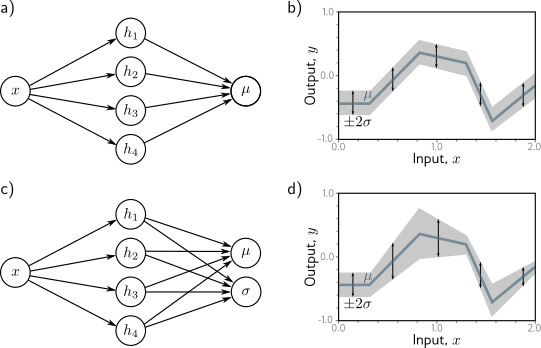
\includegraphics[width=0.7\linewidth]{png/chapter5/LossHeteroscedastic.png}
	\caption{同方差回归与异方差回归比较。a) 在同方差回归中,一个简单的神经网络模型根据输入 x 预测输出分布的平均值 μ。b) 这种情况下,尽管输出的均值(用蓝线表示)随输入 x 呈分段线性变化,方差却始终保持不变(通过箭头和灰色区域表示的 ±2 标准差来展示)。c) 异方差回归的浅层神经网络除了预测均值外,还会预测输出的方差 \(\sigma_2\)(更精确地说,是计算方差的平方根,然后再平方)。d) 如此一来,标准差也随输入 x 呈分段线性变化。}
\end{figure}

\begin{figure}[ht!]
	\centering
	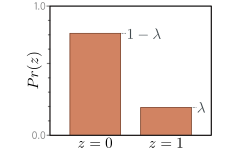
\includegraphics[width=0.7\linewidth]{png/chapter5/LossBern.png}
	\caption{伯努利分布。伯努利分布是定义在仅包含 {0,1} 的域上的分布,它由单一参数\(\lambda\)定义,\(\lambda\) 表示观测到结果为 1 的概率。相应地,结果为 0 的概率则为 \(1 − \lambda\)。}
\end{figure}

\begin{figure}[ht!]
	\centering
	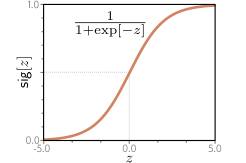
\includegraphics[width=0.7\linewidth]{png/chapter5/LossLogisticSigmoid.png}
	\caption{逻辑 Sigmoid 函数。该函数把实数 z 映射到 0 到 1 之间的值,因此 sig[z] 的范围是 [0, 1]。当输入为 0 时,输出值为 0.5。负数输入对应于小于 0.5 的输出值,而正数输入对应于大于 0.5 的输出值。}
\end{figure}



我们再次按照第5.2节的步骤构建损失函数。首先,我们为输出空间 \(y \in \{0, 1\}\) 选择了伯努利分布,这个分布定义在 \(\{0, 1\}\) 上。它有一个参数 \(\lambda \in [0, 1]\),表示 \(y\) 取值为 1 的概率(见图 5.6):

\begin{equation}
Pr(y|\lambda) = 
\begin{cases} 
	1 - \lambda & \text{if } y = 0 \\
	\lambda & \text{if } y = 1  
\end{cases} 
\end{equation}

也可以写成:

\begin{equation}
Pr(y|\lambda) = (1 - \lambda)^{1-y} \cdot \lambda^y 
\end{equation}
然后,我们设置机器学习模型 \(f(x, \phi)\) 来预测单一参数 \(\lambda\)。但由于 \(\lambda\) 只能在 [0, 1] 范围内取值,我们需要通过一个函数将网络输出映射到这个范围内。一个合适的函数是逻辑斯蒂 sigmoid 函数(见图 5.7):

\begin{equation}
sig[z] = \frac{1}{1 + \exp[-z]} 
\end{equation}
因此,我们预测的分布参数为 \(\lambda = sig[f(x, \phi)]\)。现在的似然表达式为:

\begin{equation}
Pr(y|x) = (1 - sig[f(x, \phi)])^{1-y} \cdot sig[f(x, \phi)]^y 
\end{equation}
这在图 5.8 中展示了一个浅层神经网络模型。损失函数是训练集的负对数似然:

\begin{equation}
L[\phi] = \sum_{i=1}^{I} -\left[(1 - y_i) \log [1 - sig[f(x_i, \phi)]] + y_i \log [sig[f(x_i, \phi)]]\right] 
\end{equation}
由于第5.7节将会解释的原因,这称为二元交叉熵损失。

变换后的模型输出 \(sig[f(x, \phi)]\) 预测了伯努利分布的参数 \(\lambda\)。这代表 \(y = 1\) 的概率,所以 \(1 - \lambda\) 代表 \(y = 0\) 的概率。在进行推断时,如果我们需要 \(y\) 的具体估计,那么当 \(\lambda > 0.5\) 时我们设定 \(y = 1\),否则设定 \(y = 0\)。


\begin{figure}[ht!]
	\centering
	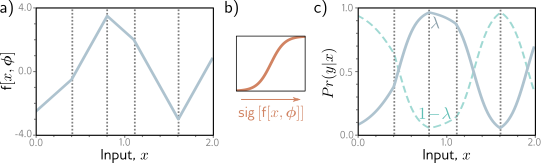
\includegraphics[width=0.7\linewidth]{png/chapter5/LossBinaryClassification.png}
	\caption{二元分类模型。a) 网络的输出是一个分段线性函数,能够接受任意实数值。b) 这些值通过逻辑 Sigmoid 函数转换,被压缩到 [0,1] 的区间内。c) 转换后的输出用来预测概率 \(\lambda\),即 y = 1 的可能性(用实线表示)。因此,y = 0 的可能性就是 \(1 − \lambda\)(用虚线表示)。对任一固定的 x(通过垂直切片展示),我们能得到一个与图 5.6 类似的伯努利分布的两种概率值。损失函数倾向于优化模型参数,使得在与正例 yi = 1 关联的 xi 位置上\(\lambda\)的值较大,而在与负例 yi = 0 关联的位置上\(\lambda\)的值较小。}
\end{figure}


\begin{figure}[ht!]
	\centering
	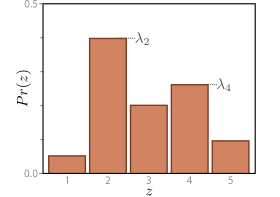
\includegraphics[width=0.7\linewidth]{png/chapter5/LossCategorical.png}
	\caption{分类分布。分类分布为超过两个的 K 类别分配概率值,相应的概率为 \(\lambda_1,\lambda_2,...,\lambda_K\)。这里有五个类别,因此 K = 5。为保证其为一个有效的概率分布,每个参数 \(\lambda_k\) 都应处于 [0, 1] 的范围内,并且所有 K 个参数的总和必须等于 1。}
\end{figure}


\section{示例 3:多类别分类}

多类别分类的目标是将输入数据 \(x\) 分配给 \(K > 2\) 个类别中的一个,即 \(y \in \{1, 2, \ldots, K\}\)。现实中的例子包括:(i)预测手写数字图像 \(x\) 中的哪一个数字 \(y\)(\(K = 10\));(ii)预测不完整句子 \(x\) 后面跟随的哪一个词汇 \(y\)(\(K\) 个可能词汇)。

我们再次遵循第5.2节的步骤。首先,对于输出空间 \(y \in \{1, 2, \ldots, K\}\),我们选择分类分布(见图 5.9)。这个分布有 \(K\) 个参数 \(\lambda_1, \lambda_2, \ldots, \lambda_K\),它们确定每个类别的概率:
\begin{equation}
Pr(y = k) = \lambda_k 
\end{equation}
参数被限制在零和一之间,并且总和必须为一,以形成有效的概率分布。

\begin{figure}[ht!]
	\centering
	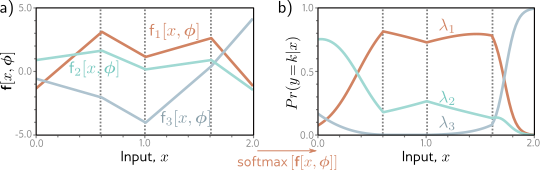
\includegraphics[width=0.7\linewidth]{png/chapter5/LossMultiClassClassification.png}
	\caption{针对 K = 3 类别的多类别分类。a) 该网络输出三个可以任意取值的分段线性函数。b) 通过 softmax 函数处理后,这些输出值被限制为非负数,且它们的总和必须为一。因此,对于任何给定的输入 x,我们都能得到有效的分类分布参数:图中任意垂直切片所产生的三个值的总和为一,这些值代表在类似图 5.9 的分类分布条形图中各条的高度。}
\end{figure}


然后,我们利用具有 \(K\) 个输出的网络 \(f(x, \phi)\) 来从输入 \(x\) 计算这 \(K\) 个参数。为了确保网络输出符合约束,我们通过一个函数处理这 \(K\) 个输出,这个函数是*softmax*函数(见图 5.10)。softmax 函数接受长度为 \(K\) 的任意向量,并返回一个同样长度的向量,其元素位于 [0, 1] 范围内且总和为一。softmax 函数的第 \(k\) 个输出是:

\begin{equation}
softmax_k[z] = \frac{\exp[z_k]}{\sum_{k'=1}^{K} \exp[z_{k'}]} 
\end{equation}
指数函数确保输出为正,分母的求和则保证这 \(K\) 个数的总和为一。

因此,输入 \(x\) 有标签 \(y\) 的似然(见图 5.10)是:

\begin{equation}
Pr(y = k|x) = softmax_k[f(x, \phi)] 
\end{equation}
损失函数是训练数据的负对数似然:

\begin{equation}
L[\phi] = -\sum_{i=1}^{I} \log \left[ softmax_{y_i} [f(x_i, \phi)] \right]
= -\sum_{i=1}^{I} \left[ f_{y_i}[x_i, \phi] - \log \left( \sum_{k'=1}^{K} \exp [f_{k'}[x_i, \phi]] \right) \right],
\end{equation}


其中 \(f_k[x, \phi]\) 是神经网络的第 \(k\) 个输出。由于将在第5.7节中解释的原因,这被称为多类别交叉熵损失。

模型输出的变换代表了 \(y \in \{1, 2, \ldots, K\}\) 可能类别的分类分布。作为点估计,我们选择最可能的类别 \(\hat{y} = argmax_k[Pr(y = k|f(x, \phi))]\),这对应于图 5.10 中对于该 \(x\) 值最高的曲线。

\subsection{预测其他数据类型}

本章主要关注回归和分类,因为这些问题非常普遍。然而,为了预测不同类型的数据,我们只需选择适合该领域的分布,并应用第5.2节中的方法。图 5.11 列出了一系列概率分布及其预测领域。其中一些将在本章末尾的问题中进行探讨。

\section{多输出预测}
在许多情况下,我们需要使用同一个模型进行多个预测,因此目标输出 \(y\) 是向量形式。例如,我们可能想同时预测分子的熔点和沸点(多变量回归问题),或者预测图像中每个点的物体类别(多变量分类问题)。虽然可以定义多变量概率分布,并利用神经网络模拟它们作为输入的函数参数,但更常见的做法是将每个预测视为独立的。

独立性意味着我们把概率 \(Pr(y|f(x, \phi))\) 看作是对于每个元素 \(y_d \in y\) 的单变量项的乘积:

\begin{equation}
Pr(y|f(x, \phi)) = \prod_{d} Pr(y_d|f_d[x, \phi]) 
\end{equation}
其中 \(f_d[x, \phi]\) 是网络对于 \(y_d\) 分布参数的第 \(d\) 组输出。例如,对于预测多个连续变量 \(y_d \in \mathbb{R}\),我们对每个 \(y_d\) 使用正态分布,并由网络输出 \(f_d[x, \phi]\) 预测这些分布的均值。对于预测多个离散变量 \(y_d \in \{1, 2, \ldots, K\}\),我们对每个 \(y_d\) 使用分类分布。在这种情况下,每组网络输出 \(f_d[x, \phi]\) 预测对 \(y_d\) 分类分布的贡献值。

最小化负对数概率时,这个乘积变为各项的求和:

\begin{equation}
L[\phi] = -\sum_{i=1}^{I} \log [Pr(y_i|f(x_i, \phi))] = -\sum_{i=1}^{I} \sum_{d} \log [Pr(y_{id}|f_d[x_i, \phi])] 
\end{equation}

其中 \(y_{id}\) 是第 \(i\) 个训练样本的第 \(d\) 个输出。

为了同时进行两种或更多类型的预测,我们同样假设每种错误是独立的。比如,为了同时预测风向和风力,我们可能分别选择定义在圆形域的 von Mises 分布预测风向,以及定义在正实数上的指数分布预测风力。独立性假设意味着这两个预测的联合似然是单独似然的乘积。在计算负对数似然时,这些项会转化为加和形式。

\begin{figure}[ht!]
	\centering
	\includegraphics[width=0.7\linewidth]{png/chapter5/511.png}
	\caption{不同预测类型下损失函数的分布。}
\end{figure}


\begin{figure}[ht!]
	\centering
	\includegraphics[width=0.7\linewidth]{png/chapter5/LossCrossEntropy.png}
	\caption{交叉熵方法。a) 训练样本的实证分布(箭头标示了 Dirac delta 函数)。b) 模型分布(参数为 \(\theta = \mu, \sigma2\) 的正态分布)。通过交叉熵方法,我们尝试最小化这两个分布之间的距离(即 KL 散度),这个距离是模型参数 \(\theta\) 的函数。}
\end{figure}



\section{交叉熵损失 (Cross-entropy loss)}

在本章中,我们开发了旨在最小化负对数似然 (negative log-likelihood) 的损失函数。然而,术语“交叉熵损失 (cross-entropy loss)”也广为流传。在本节中,我们将解释交叉熵损失,并证明它与使用负对数似然是等价的。

交叉熵损失的核心思想是寻找参数 \(\theta\),以最小化观测数据 \(y\) 的经验分布 \(q(y)\) 与模型分布 \(Pr(y|\theta)\)(见图 5.12)之间的差距。可以用 Kullback-Leibler (KL) 散度来衡量两个概率分布 \(q(z)\) 和 \(p(z)\) 之间的距离:

\begin{equation}
D_{KL}(q||p) = \int_{-\infty}^{\infty} q(z) \log [q(z)] dz - \int_{-\infty}^{\infty} q(z) \log [p(z)] dz 
\end{equation}
设想我们在点集 \(\{y_i\}^I_{i=1}\) 观测到了一组经验数据分布。这可以表示为点质量的加权总和:

\begin{equation}
q(y) = \frac{1}{I} \sum_{i=1}^{I} \delta[y - y_i] 
\end{equation}

这里的 \(\delta[\cdot]\) 是 Dirac delta 函数。我们的目标是最小化模型分布 \(Pr(y|\theta)\) 与这一经验分布之间的 KL 散度:


\begin{align}
	\hat{\theta} &= argmin_{\theta} \left[ \int_{-\infty}^{\infty} q(y) \log [q(y)] dy - \int_{-\infty}^{\infty} q(y) \log [Pr(y|\theta)] dy \right] \\
	&= argmin_{\theta} \left[ -\int_{-\infty}^{\infty} q(y) \log [Pr(y|\theta)] dy \right], 
\end{align}


由于第一项与 \(\theta\) 无关,因此消失了。剩下的第二项被称为*交叉熵 (cross-entropy)*。它可以理解为在考虑到另一个分布已知信息后,一个分布中剩余的不确定性量。接下来,我们将方程 5.28 中的 \(q(y)\) 定义代入:


\begin{align}
	\hat{\theta} &= argmin_{\theta} \left[ \int_{-\infty}^{\infty} \left( \frac{1}{I} \sum_{i=1}^{I} \delta[y - y_i] \right) \log [Pr(y|\theta)] dy \right] \\
	&= argmin_{\theta} \left[ -\sum_{i=1}^{I} \log [Pr(y_i|\theta)] \right], 
\end{align} 


第一行的两项相乘,对应于图 5.12a 中点质量与图 5.12b 中分布的对数进行逐点乘积。最终我们得到一组集中在数据点上的有限加权概率质量。在最后一行,我们去掉了不影响最小值位置的常数缩放因子 \(1/I\)。

在机器学习领域,分布参数 \(\theta\) 由模型 \(f[x_i, \phi]\) 计算得出。因此,我们有:

\begin{equation}
\hat{\phi} = argmin_{\phi} \left[ -\sum_{i=1}^{I} \log [Pr(y_i|f[x_i, \phi])] \right] 
\end{equation}
这正是第 5.2 节提到的负对数似然准则。由此可见,负对数似然准则(即最大化数据似然)与交叉熵准则(即最小化模型与经验数据分布间的距离)是等价的。

\section{总结}

在前面的章节中,我们考虑神经网络是如何直接从数据 x 预测输出 y 的。在本章,我们改变了观点,把神经网络视为计算输出空间概率分布 \(Pr(y|\theta)\) 上的参数 \(\theta\)。这引领我们采用了一种原理性方法构建损失函数。我们选择了能够使观测数据在这些分布下的似然最大化的模型参数 \(\phi\)。我们发现,这等同于最小化负对数似然 (negative log-likelihood)。

这种方法的自然结果是,回归的最小二乘准则;它基于假设 y 符合正态分布,并且我们正在预测其均值。我们还探讨了如何 (1) 扩展回归模型以估计对预测的不确定性,以及 (2) 扩展模型使不确定性依赖于输入(heteroscedastic model)。我们将同样的方法应用于二元分类和多类分类,为每种情况推导出了损失函数。我们讨论了如何处理更加复杂的数据类型以及如何处理多个输出。最后,我们指出交叉熵是另一种等效的考虑模型拟合方式。

在之前的章节中,我们开发了神经网络模型。在本章,我们为决定模型如何根据一组给定参数描述训练数据的效果,开发了损失函数。下一章将考虑模型训练,我们的目标是找到能使这种损失最小化的模型参数。


\section{Notes}

基于正态分布的损失函数:Nix \& Weigend (1994) 和 Williams (1996) 研究了异方差非线性回归 (heteroscedastic nonlinear regression),其中输出的均值和方差都是输入的函数。在无监督学习的背景下,Burda 等人 (2016) 使用了基于具有对角协方差的多变量正态分布的损失函数,而 Dorta 等人 (2018) 使用了基于具有完全协方差的正态分布的损失函数。

稳健回归:Qi 等人 (2020) 研究了最小化平均绝对误差而非平均平方误差的回归模型特性。这种损失函数基于对输出采用拉普拉斯分布的假设,并估计给定输入的中位数输出,而非均值。Barron (2019) 提出了一种参数化稳健度的损失函数。在概率背景下解释时,它产生了一个包括正态分布和柯西分布作为特例的单变量概率分布族。

估计分位数:有时,我们可能不想在回归任务中估计均值或中位数,而是希望预测一个分位数。例如,这对风险模型很有用,我们希望知道真实值在 90% 的时间内会小于预测值。这被称为分位数回归 (Koenker & Hallock, 2001)。这可以通过拟合一个异方差回归模型,然后基于预测的正态分布估计分位数来完成。或者,分位数可以直接使用分位数损失(也称为弹球损失)来估计。在实践中,这最小化了数据与模型的绝对偏差,但在一个方向上对偏差的权重比另一个方向更大。最近的研究探索了同时预测多个分位数以获得整体分布形状的概念(Rodrigues & Pereira, 2020)。

类别不平衡和焦点损失:Lin 等人 (2017c) 讨论了分类问题中的数据不平衡问题。如果某些类别的示例数量远大于其他类别,则标准的最大似然损失就不再适用;模型可能会专注于提高对主导类别中已分类良好示例的信心,而对代表性较差的类别分类不佳。Lin 等人 (2017c) 引入了焦点损失,该损失添加了一个额外的参数,用于减弱分类良好示例的影响,以提高性能。

学习排名:Cao 等人 (2007),Xia 等人 (2008),和 Chen 等人 (2009) 都在学习排名数据的损失函数中使用了 Plackett-Luce 模型。这是学习排名的列表式方法,因为模型一次性处理整个待排名的对象列表。其他方法包括点式方法,其中模型处理单个对象,以及对式方法,其中模型处理对象对。Chen 等人 (2009) 总结了学习排名的不同方法。

其他数据类型:Fan 等人 (2020) 使用基于贝塔分布的损失来预测 0 到 1 之间的值。Jacobs 等人 (1991) 和 Bishop (1994) 研究了适用于多模态数据的混合密度网络。这些模型将输出建模为基于输入的高斯混合(见图 5.14)。Prokudin 等人 (2018) 使用了 von Mises 分布来预测方向(见图 5.13)。Fallah 等人 (2009) 使用泊松分布构建了预测计数的损失函数(见图 5.15)。Ng 等人 (2017) 使用基于伽马分布的损失函数来预测持续时间。

\begin{figure}[ht!]
	\centering
	\includegraphics[width=0.7\linewidth]{png/chapter5/LossVonMises.png}
	\caption{Figure5.13}
\end{figure}

`图 5.13 冯·米塞斯分布定义在圆周上,范围是 \((−\pi, \pi]\)。它由两个参数构成:平均值 \(\mu\) 决定了分布峰值的位置;浓度参数 K(大于 0)起着类似于方差倒数的作用,因此 \(\frac{1}{\sqrt{\kappa}}\) 可以大致看作是与正态分布的标准差相对应的量。`

非概率方法:采用本章讨论的概率方法并不是严格必要的,但这在近年来已成为默认方法;任何旨在减少模型输出与训练输出之间距离的损失函数都是足够的,距离可以用任何看似合理的方式定义。有几种著名的非概率机器学习模型用于分类,包括支持向量机 (Vapnik, 1995; Cristianini \& Shawe-Taylor, 2000),它们使用铰链损失,以及 AdaBoost (Freund \& Schapire, 1997),它们使用指数损失。


\section{习题}

\textbf{问题 5.1} 证明逻辑 sigmoid 函数 \(\text{sig}[z]\) 将 \(z = -\infty\) 映射到 0,\(z = 0\) 映射到 0.5,\(z = \infty\) 映射到 1,其中:

\begin{equation}
\text{sig}[z] = \frac{1}{1 + \exp[-z]} 
\end{equation}

\textbf{问题 5.2} 对于单个训练对 \(\{x, y\}\) 的二元分类,损失 \(L\) 为:

\begin{equation}
L = -(1 - y) \log [1 - \text{sig}[f[x, \phi]]] - y \log [\text{sig}[f[x, \phi]]] 
\end{equation}
其中 \(\text{sig}[\cdot]\) 在方程 5.32 中定义。当训练标签 \(y = 0\) 时(1)以及当 \(y = 1\) 时(2),将这种损失作为变换后的网络输出 \(\text{sig}[f[x, \phi]] \in [0, 1]\) 的函数绘制出来。 \\


\textbf{问题 5.3}* 假设我们想构建一个模型,基于本地气压 \(x\) 的测量来预测占主导地位的风向 \(y\)(以弧度表示)。适用于圆形域的分布是 von Mises distribution(见图 5.13):

\begin{equation}
Pr(y|\mu, \kappa) = \frac{\exp[\kappa \cos(y - \mu)]}{2\pi \cdot \text{Bessel}_0[\kappa]} 
\end{equation}
其中 \(\mu\) 是平均方向的度量,\(\kappa\) 是集中度的度量(即方差的倒数)。项 \(\text{Bessel}_0[\kappa]\) 是阶数为 0 的修改过的贝塞尔函数。使用第 5.2 节的配方来开发用于学习模型 \(f[x, \phi]\) 参数 \(\mu\) 的损失函数,以预测最有可能的风向。你的解决方案应将集中度 \(\kappa\) 视为常数。你会如何进行推理? \\

\textbf{问题 5.4}* 有时,对于输入 \(x\) 的输出 \(y\) 是多模态的(见图 5.14a);对于给定输入,有多个有效的预测。在这里,我们可能使用正态分量的加权和作为输出的分布。这被称为高斯混合 (Gaussian Mixture) 模型。例如,两个高斯的混合具有参数 \(\Theta = \{\lambda, \mu_1, \sigma_1^2, \mu_2, \sigma_2^2\}\):

\begin{equation}
Pr(y|\mu_1, \mu_2, \sigma_1^2, \sigma_2^2) = \frac{\lambda}{\sqrt{2\pi\sigma_1^2}} \exp \left[ -\frac{(y - \mu_1)^2}{2\sigma_1^2} \right] + \frac{1 - \lambda}{\sqrt{2\pi\sigma_2^2}} \exp \left[ -\frac{(y - \mu_2)^2}{2\sigma_2^2} \right] 
\end{equation}
其中 \(\lambda \in [0, 1]\) 控制两个分量的相对权重,它们分别具有均值 \(\mu_1, \mu_2\) 和方差 \(\sigma_1^2, \sigma_2^2\)。这个模型可以表示具有两个峰的分布(见图 5.14b)或具有更复杂形状的单峰分布(见图 5.14c)。使用第 5.2 节的配方构建一个训练模型 \(f[x, \phi]\) 的损失函数,该模型接收输入 \(x\),具有参数 \(\phi\),并预测两个高斯的混合。损失应基于 \(I\) 训练数据对 \(\{x_i, y_i\}\)。在进行推理时,你预见会遇到什么问题?

\begin{figure}[ht!]
	\centering
	\includegraphics[width=0.7\linewidth]{png/chapter5/LossMoG.png}
	\caption{多模态数据及其高斯混合密度。 a) 在示例训练数据中,当输入 x 的值处于中间范围时,相应的输出 y 会沿着两种可能的路径之一变化。例如,在 x = 0 的情况下,输出 y 的值可能接近 −2 或 +3,但不太可能是介于这两个值之间。b) 高斯混合模型非常适合描述这种数据,它通过将两个或更多具有不同均值和方差的正态分布(此处为两个分布,分别用虚线蓝色和橙色曲线表示)进行加权求和(用实线青色曲线表示)来构建。当各个正态分布的均值相差较远时,便形成了多模态分布。c) 当这些均值较为接近时,这种混合模型能够描述单峰但非正态的密度分布。}
\end{figure}


\textbf{问题 5.5} 考虑扩展问题 5.3 中的模型,使用两个 von Mises distribution 的混合来预测风向。为这个模型写出似然 \(Pr(y|\theta)\) 的表达式。网络需要产生多少个输出?

\textbf{问题 5.6} 考虑构建一个模型,预测接下来一分钟内将有多少行人 \(y \in \{0, 1, 2, \ldots\}\) 经过城市中给定的点,这是基于包含一天中的时间、经纬度和社区类型等信息的数据 \(x\)。适用于模拟计数的分布是泊松分布(见图 5.15)。它有一个称为速率的单一参数 \(\lambda > 0\),代表分布的均值。该分布的概率密度函数为:

\begin{equation}
Pr(y = k) = \frac{\lambda^k e^{-\lambda}}{k!} 
\end{equation}
假设我们可以访问 \(I\) 个训练对 \(\{x_i, y_i\}\),为这个模型设计一个损失函数。

\begin{figure}[ht!]
	\centering
	\includegraphics[width=0.7\linewidth]{png/chapter5/LossPoisson.png}
	\caption{泊松分布是定义在非负整数上的离散分布,具有一个参数 \(\lambda\)(正实数),称为分布的率,它代表了分布的平均值。a–c) 分别展示了当率为 1.4、2.8 和 6.0 时的泊松分布,展示了不同率值下分布形态的变化。}
\end{figure}


\textbf{问题 5.7} 考虑一个多变量回归问题,我们预测十个输出,因此 \(y \in \mathbb{R}^{10}\),并且用独立的正态分布对每个进行建模,其中均值 \(\mu_d\) 由网络预测,方差 \(\sigma^2\) 是常数。写出似然 \(Pr(y|f[x, \phi])\) 的表达式。展示如果我们不估计方差 \(\sigma^2\),最小化这个模型的负对数似然仍然等价于最小化一系列平方项。

\textbf{问题 5.8}* 构建一个损失函数,用于基于独立正态分布进行多变量预测 \(y \in \mathbb{R}^D_i\),每个维度有不同的方差 \(\sigma_d^2\)。假设一个异方差模型,使得均值 \(\mu_d\) 和方差 \(\sigma_d^2\) 都随数据而变化。

\textbf{问题 5.9}* 考虑一个多变量回归问题,我们从数据 \(x\) 预测一个人的身高(以米为单位)和体重(以千克为单位)。这里,单位的范围差异较大。你认为这会导致什么问题?提出两个解决这些问题的方案。

\textbf{问题 5.10} 扩展问题 5.3 中的模型,预测风向和风速,并定义相关的损失函数。

\chapter{训练模型}
第 3 章和第 4 章详细讨论了浅层和深层神经网络,它们构成了分段线性函数族,函数的具体形式由各自的参数确定。第 5 章引入了损失概念 —— 一个反映网络预测与训练集真实值差异的单个数值。
损失与网络参数有关,本章着重于探讨如何确定能使损失最小化的参数值。这个过程称为网络参数的学习,或更通俗地说,是模型的训练或拟合。该过程首先是选取一组初始参数值,随后重复执行两个步骤:(i) 计算损失函数关于参数的导数(梯度);(ii) 根据梯度调整参数,以期减少损失。多次迭代后,目标是使损失函数达到其全局最小值。
本章重点讨论参数调整步骤,即采用何种算法来减少损失。第 7 章将介绍如何为神经网络初始化参数并计算梯度。
\section{梯度下降}
为了拟合模型,我们需要一组输入/输出对的训练集 \(\{x_i, y_i\}\)。我们寻求模型 \(f(x_i, \phi)\) 的参数 \(\phi\),使得这些参数能够尽可能准确地将输入 \(x_i\) 映射到输出 \(y_i\)。为此目的,我们定义了一个损失函数 \(L(\phi)\),它通过返回一个数值来量化映射中的误差。优化算法的目标是找到一组参数 \(\hat{\phi}\),使得这个损失函数达到最小值:

\begin{equation}
\hat{\phi} = \arg\min_{\phi} L(\phi) 
\end{equation}


虽然存在多种优化算法,但训练神经网络通常采用迭代方法。这些方法首先启发式地设定初始参数值,然后反复调整参数以降低损失值。

这个过程中最基本的方法称为梯度下降。它从初始参数 \(\phi = [\phi_0, \phi_1, \ldots, \phi_N]^T\) 开始,并分两步迭代:

\textbf{步骤 1.} 计算损失相对于参数的导数:
\begin{equation}
\frac{\partial L}{\partial \phi} =
\begin{bmatrix}
\frac{\partial L}{\partial \phi_0}  \\
\frac{\partial L}{\partial \phi_1}  \\
\vdots  \\
\frac{\partial L}{\partial \phi_N} 
\end{bmatrix} 
\end{equation}

\textbf{步骤 2.} 根据以下规则更新参数:
\begin{equation}
\phi \leftarrow \phi - \alpha \cdot \frac{\partial L}{\partial \phi} 
\end{equation}
其中,正数 \(\alpha\) 确定了调整的幅度。

第一步计算当前位置上损失函数的梯度,确定了损失增加的方向。第二步则是向相反方向(即下降方向)小幅移动。参数 \(\alpha\) 可以固定(此时称之为学习率),或者通过线性搜索尝试多个 \(\alpha\) 值,以找到能最大程度降低损失的值。

当损失函数达到最小值时,其表面必须是平坦的(否则,我们还能通过继续下降来进一步改进)。因此,梯度将变为零,参数也随之停止改变。在实践中,我们会监测梯度的大小,并在其变得过小时停止算法。

\subsection{线性回归示例}

考虑将梯度下降方法应用于第2章介绍的一维线性回归模型。该模型 \(f(x, \phi)\) 把一个标量输入 \(x\) 映射到一个标量输出 \(y\),具有参数 \(\phi = [\phi_0, \phi_1]^T\),分别代表了y轴截距和斜率:

\begin{equation}
y = f(x, \phi) = \phi_0 + \phi_1x 
\end{equation}

给定一个数据集 \(\{x_i, y_i\}\),包含 \(I\) 对输入/输出数据,我们采用最小二乘法作为损失函数:
\begin{equation}
L(\phi) = \sum_{i=1}^I e_i = \sum_{i=1}^I (f(x_i, \phi) - y_i)^2 = \sum_{i=1}^I (\phi_0 + \phi_1x_i - y_i)^2 
\end{equation}
这里的 \(e_i = (\phi_0 + \phi_1x_i - y_i)^2\) 表示第 \(i\) 个训练样本对损失的单独贡献。

损失函数对参数的导数可以表示为各个贡献导数的总和:
\begin{equation}
\frac{\partial L}{\partial \phi} = \frac{\partial}{\partial \phi} \sum_{i=1}^I e_i = \sum_{i=1}^I \frac{\partial e_i}{\partial \phi} 
\end{equation}
具体计算方式如下:
\begin{equation}
\frac{\partial e_i}{\partial \phi} = 
\begin{bmatrix}
\frac{\partial e_i}{\partial \phi_0}  \\
\frac{\partial e_i}{\partial \phi_1} 
\end{bmatrix} =
\begin{bmatrix}
2(\phi_0 + \phi_1x_i - y_i)  \\
2x_i(\phi_0 + \phi_1x_i - y_i)  
\end{bmatrix} 
\end{equation}

图 6.1 通过迭代地根据方程 6.6 和 6.7 计算导数,接着依据方程 6.3 的规则更新参数,展示了算法的逐步进展。在此示例中,我们采用了线搜索技术,在每次迭代中找到能够最大限度减少损失的 \(\alpha\) 值。

\begin{figure}[ht!]
	\centering
	\includegraphics[width=0.7\linewidth]{png/chapter6/TrainLRMin.png}
	\caption{图 6.1 线性回归模型的梯度下降。a) 训练集由 12 对输入/输出数据对 {xi , yi} 组成。b) 损失函数图展示了梯度下降的迭代过程。从点 0 出发,我们沿最陡峭的下降方向前进,直至无法进一步降低损失,从而到达点 1。然后,我们重复此过程,测量点 1 的梯度并继续下降到点 2,以此类推。c) 通过热图可以更直观地展示这一过程,图中的亮度代表了损失大小。仅经过四轮迭代,我们已经非常接近最小损失值。d) 点 0 处参数(线条最浅)的模型对数据的描述非常不准确,但随着每轮迭代,模型的拟合度都有所提升。点 4 处参数(线条最深)的模型已能合理描述训练数据。}
	\end{figure}

\subsection{Gabor模型示例}
线性回归问题的损失函数(参见图 6.1c)总是有一个清晰定义的全局最小值。更形式化地说,这些函数是凸函数,意味着曲面上任意两点连线(即弦)不会穿过函数图像。凸性保证了无论参数初始化在何处,只要我们不断地“下坡”,最终都能找到最小值;这样的训练过程是不会失败的。

然而,大部分非线性模型(包括浅层和深层网络)的损失函数都是非凸的。由于参数众多,使得神经网络损失函数的可视化变得极具挑战性。因此,我们首先研究一个参数较少的简单非线性模型,以深入理解非凸损失函数的特性:

\begin{equation}
f(x, \phi) = \sin[\phi_0 + 0.06 \cdot \phi_1x] \cdot \exp \left( - \frac{(\phi_0 + 0.06 \cdot \phi_1x)^2}{32.0} \right) 
\end{equation}

这个Gabor模型将标量输入\(x\)映射到标量输出\(y\),并且由一个正弦分量(产生振荡效果)和一个负指数分量(使得振幅随离中心距离增加而减小)相乘构成。模型具有两个参数\(\phi = [\phi_0, \phi_1]^T\),\(\phi_0 \in \mathbb{R}\) 控制函数的拉伸或压缩,而\(\phi_1 \in \mathbb{R}^+\) 则决定沿x轴的拉伸或压缩(见图6.2)。

考虑一个包含\(I\)个样本\(\{x_i, y_i\}\)的训练集。定义\(I\)个训练样本的最小二乘损失函数为:
\begin{equation}
L(\phi) = \sum_{i=1}^I (f(x_i, \phi) - y_i)^2 
\end{equation}

目标再次是找到能够最小化这个损失的参数\(\hat{\phi}\)。

\begin{figure}[ht!]
\centering
\includegraphics[width=0.7\linewidth]{png/chapter6/TrainGaborModel.png}
\caption{图 6.2 Gabor 模型。这个非线性模型将单一输入 x 映射到单一输出 y,拥有参数组\(\phi= [\phi_0 , \phi_1]T\)。它描述了一个振幅随距离中心增加而减小的正弦波函数。\(\phi_0\) 参数决定了波峰的位置,随 \(\phi_0\) 增大,波形向左移动。\(\phi_1\) 参数控制波形相对于中心的压缩程度,\(\phi_1\) 增大时,波形变得更窄。a–c) 展示了具有不同参数的模型。}
\end{figure}
	
\begin{figure}[ht!]
\centering
\includegraphics[width=0.7\linewidth]{png/chapter6/TrainGaborData.png}
\caption{图 6.3 用于拟合 Gabor 模型的训练数据。训练集包含了 28 组输入/输出样本 {xi,yi}。这些样本是通过在区间 [−15, 15] 内均匀采样 xi,然后将样本值通过参数设为\(\phi\)= [0.0,16.6]T 的 Gabor 模型处理,并加入正态分布的噪声生成的。}
\end{figure}

\subsection{局部最小值与鞍点}
图 6.4 展示了这个数据集的 Gabor 模型损失函数。存在众多局部最小值(标记为青色圆圈)。在这些位置,梯度为零,无论向哪个方向移动,损失都会增加,然而这些并不代表函数的全局最小点。损失最小的点,即全局最小值,用灰色圆圈标出。

如果我们从随机位置出发,采用梯度下降法“下山”,无法保证最终能够达到全局最小值并找出最优参数(参见图 6.5a)。算法很可能会停在某个局部最小值,而不是最佳解。更重要的是,我们无法确定是否有更优的解存在于其他地方。

此外,损失函数中还存在鞍点(比如图 6.4中的蓝色十字处)。在鞍点,虽然梯度为零,但是函数值在某些方向上升,在其他方向下降。如果当前参数位置并非正好在鞍点上,那么通过“下山”梯度下降法仍有可能逃脱。然而,鞍点附近的曲面几乎是平坦的,这使得很难确定训练是否已经收敛。如果我们在梯度很小时就终止算法,可能会错误地在鞍点附近停止,误以为找到了解决方案。


\begin{figure}[ht!]
\centering
\includegraphics[width=0.7\linewidth]{png/chapter6/TrainGaborMin.png}
\caption{Gabor 模型的损失函数。a) 损失函数呈现非凸形状,除了一个全局最小值(灰色圆圈)外,还存在多个局部最小值(青色圆圈)。同时,该函数包含鞍点,即在这些点上,虽然梯度临时为零,但函数值在某一方向上升,在另一方向下降。例如,蓝色叉号标识的鞍点,水平方向移动导致函数值下降,而垂直方向移动则导致上升。b–f) 展示了对应于不同最小值点的模型状态。在这些状态下,任何微小的调整都无法使损失值进一步降低。图 (c) 中展示的全局最小值点,其损失值为 0.64。}
\end{figure}

\begin{figure}[ht!]
\centering
\includegraphics[width=0.7\linewidth]{png/chapter6/TrainGaborGDSGD.png}
\caption{梯度下降与随机梯度下降的比较。a) 使用线性搜索的梯度下降方法。只要初始设置正确,位于损失函数的适当“谷底”(如点 1 和 3),参数估计便会稳步向全局最小值靠拢。但如果初始点设在这个谷底之外(如点 2),则可能会陷入局部最小值。b) 随机梯度下降通过引入噪声到优化过程中,使得即便是从错误的“谷底”(如点 2)出发,也有可能跳出并最终找到全局最小值。}
\end{figure}

\section{随机梯度下降}
Gabor 模型具有两个参数,因此我们可以通过以下两种方式找到全局最小值:(i)穷尽地搜索参数空间或(ii)重复从不同位置开始梯度下降,并选择损失最低的结果。然而,神经网络模型可能拥有数以百万计的参数,这使得上述两种方法都不现实。简言之,利用梯度下降方法寻找高维损失函数的全局最优解颇具挑战性。我们能找到一个最小值,但无法确定这是否为全局最小值或一个较优解。
一个主要问题是,梯度下降算法的最终结果完全取决于其起始点。随机梯度下降(SGD)尝试通过在每一步中为梯度引入一些噪声来解决这一问题。这样,解决方案在平均意义上仍向低处移动,但在任何给定的迭代中,所选方向不必然是最陡峭的下坡方向。实际上,有时甚至可能不是向下的。SGD算法可能暂时向上移动,因此能够从损失函数的一个“谷”跳跃到另一个(见图 6.5b)。

\begin{figure}[ht!]
\centering
\includegraphics[width=0.7\linewidth]{png/chapter6/TrainGaborSGDIter.png}
\caption{针对 Gabor 模型的随机梯度下降方法,采用的批处理大小为三。a) 针对全部训练数据集的损失函数图。每一次迭代都对应一组可能的参数变化概率分布(小图展示了样本选择)。这些分布对应于选择的三个批处理元素的不同组合。b) 某一特定批处理的损失函数图。随机梯度下降算法依据学习速率和当前梯度的大小,沿着损失函数下降方向移动一段距离。当前模型(小图中的虚线表示)将调整以更好地符合这批数据(以实线表示)。c) 另一批数据会生成不同的损失函数,并导致不同的模型更新。d) 对这批数据,算法沿着批损失函数的下降方向移动,但相对于图 (a) 中的全局损失函数可能是上升的。这展示了随机梯度下降如何帮助模型跳出局部最小值,寻找全局最优解。}
\end{figure}

\subsection{批次和周期}
引入随机性的机制很简单。在每次迭代时,算法随机选择训练数据的一个子集,并仅根据这些示例计算梯度。这个子集称为*小批量*(minibatch)或简称*批次*(batch)。因此,模型参数\(\phi_t\)在第t次迭代的更新规则为:
\begin{equation}
\phi_{t+1} \leftarrow \phi_t - \alpha \cdot \sum_{i \in B_t} \frac{\partial \mathcal{L}[\phi]}{\partial \phi} 
\end{equation}
其中\(B_t\)是当前批次中输入/输出对索引的集合,\(e_i\)是第\(i\)对导致的损失。\(\alpha\)是学习率,与梯度大小一起,决定了每次迭代的移动距离。学习率在开始时确定,并不受函数局部特性的影响。

通常,批次是从数据集中不重复抽取的。算法遍历所有训练样本直至全部使用完毕,然后再次从完整训练数据集开始抽样。整个训练数据集的单次遍历称为一个*周期*。批次的大小可以从单一样本到整个数据集不等。后者被称为*全批量梯度下降*,与常规(非随机)梯度下降相同。

SGD的另一解释是,它在每次迭代计算不同损失函数的梯度;由于损失函数依赖于模型与训练数据,因此每个随机选择的批次都会不同。从这个角度看,SGD在一个不断变化的损失函数上执行确定性梯度下降(见图 6.6)。然而,尽管存在这种变异性,任何点的期望损失和梯度与常规梯度下降保持一致。


\subsection{随机梯度下降的特性}
SGD具有几个吸引人的特点。首先,尽管它在路径上增加了噪声,但每次迭代都改善了对数据子集的拟合,因此更新通常是合理的,即使不是最佳的。其次,通过无重复抽取训练样本并遍历数据集,保证了所有训练样本的平等贡献。第三,仅使用训练数据的一部分计算梯度在计算上更为高效。第四,它原则上能够逃离局部最小值。第五,它减少了在鞍点附近停滞的几率;很可能至少有一些批次在损失函数的任何点上都有显著梯度。最后,有证据表明,SGD找到的参数能使神经网络在实际中对新数据具有良好的泛化能力(见第9.2节)。

SGD不一定按传统意义上“收敛”。然而,我们希望当接近全局最小值时,所有数据点都能被模型很好地描述,这样无论选择哪个批次,梯度都将很小,参数变化不大。实践中,SGD常配合学习率调度使用。学习率 \(\alpha\) 起始于一个较高值,并每经过N个周期以一个固定比例降低。这样做的逻辑是,在训练初期,我们希望算法能探索参数空间,跨越不同的“谷”寻找合理的区域;而在后期,当我们大致处于正确位置时,更注重参数的微调,因此通过降低 \(\alpha\) 来减小变化幅度。

\section{动量}
在随机梯度下降法中,增加动量(Momentum)项是一种常见的改进方法。此方法通过结合当前批次计算得到的梯度与上一步骤的移动方向的加权组合来更新参数:
\begin{align}
& m_{t+1} \leftarrow \beta \cdot m_t + (1 - \beta) \sum_{i \in B_t} \frac{\partial \mathcal{L}[\phi]}{\partial \phi} \notag \\
& \phi_{t+1} \leftarrow \phi_t - \alpha \cdot m_{t+1},
\end{align}

其中,\(m_t\) 表示动量项,\(\beta \in [0,1]\) 用于控制随时间变化的平滑效果,\(\alpha\) 为学习率。

动量的递归计算方式导致梯度更新步骤成为所有先前梯度的无限加权和,其中随着时间的推移,权重逐渐减少。若这些梯度在多个迭代中保持一致方向,则有效的学习速率会增加;反之,如果梯度方向频繁变化,由于累加项之间的相互抵消,有效的学习速率则会降低。这样能够使参数更新路径更加平滑,减少在优化过程中的震荡现象(参见图 6.7)。

\subsection{Nesterov 加速动量}
动量项可视为对 SGD 算法下一步移动位置的粗略预测。Nesterov 加速动量(参见图 6.8)不是在当前位置,而是在预测的位置计算梯度:


\begin{align}
& m_{t+1} \leftarrow \beta \cdot m_t + (1 - \beta) \sum_{i in B} \frac{\partial L(\phi_t - \alpha \cdot m_t)}{\partial \phi} \notag \\
& \phi_{t+1} \leftarrow \phi_t - \alpha \cdot m_{t+1} 
\end{align} 


此处,梯度是在 \(\phi_t - \alpha \cdot m_t\) 位置计算的。这种方式使得梯度项能够对仅靠动量确定的路径进行修正。

\begin{figure}[ht!]
\centering
\includegraphics[width=0.7\linewidth]{png/chapter6/TrainMomentum.png}
\caption{带动量的随机梯度下降。a) 传统的随机梯度下降方法向最小值进发的路径曲折复杂。b) 通过引入动量项,可以将当前步的更新设定为之前更新与当前批次梯度的加权混合,从而使路径更平滑,加快收敛速度。}
\end{figure}

\begin{figure}[ht!]
\centering
\includegraphics[width=0.7\linewidth]{png/chapter6/TrainNesterov.png}
\caption{Nesterov 加速动量。该方法的解沿虚线前进至点 1。在传统动量更新中,先在点 1 处计算梯度,再按此方向移动至点 2,并添加前一次迭代的动量(即延虚线方向),最终到达点 3。Nesterov 动量先应用动量(从点 1 至点 4),然后计算梯度并更新至点 5。}
\end{figure}

\section{Adam}
传统的梯度下降方法采用固定步长,存在一个问题:它会对大梯度的参数做出较大调整(在这些情况下我们可能需要更加小心),而对小梯度的参数调整较小(这里可能需要进一步的探索)。当损失函数表面的梯度在一个方向比另一个方向更陡峭时,很难选择一个同时能(i)在两个方向上有效进展且(ii)保持稳定的学习率(见图 6.9a–b)。

一个简便的方法是对梯度进行标准化处理,使得在每个方向上都能按固定距离(由学习率决定)前进。首先,我们计算梯度 \(m_{t+1}\) 和逐点平方梯度 \(v_{t+1}\):

\begin{align}
& m_{t+1} \leftarrow \frac{\partial L(\phi_t)}{\partial \phi} \notag \\
& v_{t+1} \leftarrow \left( \frac{\partial L(\phi_t)}{\partial \phi} \right)^2
\end{align}


接下来应用更新规则:

\begin{equation}
\phi_{t+1} \leftarrow \phi_t - \alpha \cdot \frac{m_{t+1}}{\sqrt{v_{t+1} + \epsilon}} 
\end{equation}

其中,平方根和除法均为逐点执行,\(\alpha\) 表示学习率,\(\epsilon\) 是一个小常量,用于防止当梯度大小为零时除以零的情况。\(v_{t+1}\) 为平方梯度,通过其正平方根来标准化梯度,使得最终只剩下每个坐标方向上的符号。算法因此沿每个坐标方向移动固定距离 \(\alpha\),方向由下坡方向确定(见图 6.9c)。这种简单的算法虽然能在两个方向上取得进展,但除非刚好到达最小值点,否则不会收敛。它会在最小值周围反复跳动。

\textit{自适应矩估计}(Adaptive Moment Estimation,简称\textit{Adam})在这一思路基础上,对梯度估计和平方梯度都引入了动量:
\begin{align}
&m_{t+1} \leftarrow \beta \cdot m_t + (1 - \beta) \frac{\partial L(\phi_t)}{\partial \phi} \notag \\
&v_{t+1} \leftarrow \gamma \cdot v_t + (1 - \gamma) \left( \frac{\partial L(\phi_t)}{\partial \phi} \right)^2
\end{align}

其中 \(\beta\) 和 \(\gamma\) 分别是两种统计量的动量系数。

使用动量相当于对这些统计量的历史数据进行加权平均。在开始时,所有之前的测量基本上都是零,这会导致估计值过小。因此,我们通过以下规则对这些统计量进行调整:

\begin{align}
& \hat{m}_{t+1} \leftarrow \frac{m_{t+1}}{1 - \beta^{t+1}} \notag \\
& \hat{v}_{t+1} \leftarrow \frac{v_{t+1}}{1 - \gamma^{t+1}} 
\end{align}


由于 \(\beta\) 和 \(\gamma\) 的取值范围是 [0,1],随着时间步进,指数项 \(t+1\) 逐渐减小,分母趋近于一,这种调整的效果逐渐变小。

最终,我们按之前的方式更新参数,但使用调整后的项:

\begin{equation}
\phi_{t+1} \leftarrow \phi_t - \alpha \cdot \frac{\hat{m}_{t+1}}{\sqrt{\hat{v}_{t+1}} + \epsilon} 
\end{equation}

这一算法能够朝整体最小值收敛,并在参数空间的每个方向上都取得良好进展。注意,Adam 通常在一个随机环境下使用,其中梯度及其平方基于小批量数据计算:

\begin{align}
&m_{t+1} \leftarrow \beta \cdot m_t + (1 - \beta) \sum_{i \in B} \frac{\partial L(\phi_t)}{\partial \phi} \notag \\
&v_{t+1} \leftarrow \gamma \cdot v_t + (1 - \gamma) \sum_{i in B} \left( \frac{\partial L(\phi_t)}{\partial \phi} \right)^2 
\end{align}

因此,实际的轨迹会有噪声。

\begin{figure}[ht!]
\centering
\includegraphics[width=0.7\linewidth]{png/chapter6/TrainADAM.png}
\caption{图 6.9 自适应矩估计(Adam)。a) 该损失函数在垂直方向上迅速变化,在水平方向上变化缓慢。若使用适合垂直进展的学习率进行全批梯度下降,算法达到最终水平位置需时甚久。b) 若学习率设置利于水平进展,则会在垂直方向过冲,导致不稳定。c) 一个简单方法是每步沿每个轴固定距离移动,以两个方向都下降。这需要通过归一化梯度大小并保留方向来完成。但这通常不会精确收敛至最小值,而是在其周边振荡(如最后两点间)。d) Adam 算法利用动量优化梯度估计和归一化,确保路径更平滑。}
\end{figure}

如第7章所述,神经网络参数的梯度大小可能取决于它们在网络中的深度。Adam 有助于补偿这一趋势,并在不同层之间平衡变化。实际上,由于它避免了图 6.9a–b 中描述的情况,Adam 对初始学习率的敏感度较低,因此不需要复杂的学习率调整策略。

\section{训练算法的超参数}
选择学习算法、批量大小(Batch Size)、学习率调度(Learning Rate Schedule)和动量系数(Momentum Coefficients)都是训练算法的超参数;它们直接影响最终模型的性能,但与模型的参数本身不同。挑选这些超参数更像是一门艺术而非精确科学,常见的做法是训练多个带有不同超参数的模型,然后选出表现最佳的一个。这个过程称为超参数搜索。我们将在第8章深入讨论这一话题。

\section{总结}
本章围绕模型训练进行了讨论。我们将问题定义为找到使损失函数 \(L[\phi]\) 达到最小的参数 \(\phi\)。梯度下降法(Gradient Descent)通过测量当前参数下损失函数的梯度(即,当我们微调参数时损失如何变化)来进行。接着,它会将参数向着能使损失最快减少的方向调整。这个过程持续进行,直到达到收敛状态。

对于非线性函数,损失函数可能存在局部最小值(梯度下降可能会陷入这些点)和鞍点(梯度下降可能似乎已收敛,但实际上并未真正收敛)。随机梯度下降(Stochastic Gradient Descent)有助于缓解这些问题。每次迭代,我们都使用数据的一个不同随机子集(一个批次)来计算梯度,为过程引入噪声,避免算法陷入参数空间的非最优区域。此外,每次迭代计算成本更低,因为只利用了数据的一部分。我们还看到,引入动量项可以使收敛过程更加高效。最后,我们介绍了 Adam 算法(Adam Algorithm)。

本章内容适用于任何模型的优化。下一章将专门探讨与神经网络训练相关的两个问题。首先是如何使用著名的反向传播算法(Backpropagation Algorithm)计算损失函数相对于神经网络参数的梯度。其次是在优化开始之前如何正确初始化网络参数。如果初始化不当,优化过程使用的梯度可能会异常大或小,从而妨碍训练进程。

\section{Notes}
\textbf{优化算法}:优化算法在工程学中被广泛使用,一般倾向于使用“目标函数”而非损失函数或成本函数。梯度下降法由 Cauchy 在 1847 年提出,而随机梯度下降的概念至少可以追溯到 Robbins \& Monro 的 1951 年工作。两者之间的一种现代中间方案是随机方差减小下降(Stochastic Variance-Reduced Descent, Johnson \& Zhang, 2013),在该方法中,全梯度定期计算,与随机更新交替进行。优化算法,特别是针对神经网络的,可以参考 Ruder (2016)、Bottou 等 (2018) 以及 Sun (2020) 的综述。Bottou (2012) 探讨了 SGD 的最佳实践,包括无重复的随机选择。

\textbf{凸性、极小值与鞍点}:如果函数上任意两点间的连线(弦)都不与函数相交,则该函数是凸的。这可以通过分析海森矩阵(Hessian Matrix,即二阶导数矩阵)来验证:
\begin{equation}
H[\phi] = \begin{bmatrix}
	\frac{\partial^2 L}{\partial \phi_0^2} & \frac{\partial^2 L}{\partial \phi_0 \partial \phi_1}  \\
	\frac{\partial^2 L}{\partial \phi_1 \partial \phi_0} & \frac{\partial^2 L}{\partial \phi_1^2}  \\
\end{bmatrix} 
\end{equation}

如果海森矩阵在所有可能的参数值上都是正定的(具有正特征值),则该函数是凸的;损失函数将呈现为光滑的碗状(如图 6.1c 所示),使得训练过程相对简单。存在单一的全局最小值,不会有局部最小值或鞍点。

对于任何损失函数,梯度为零的位置处海森矩阵的特征值能够帮助我们将该位置分类为:(i)最小值(所有特征值均为正),(ii)最大值(所有特征值均为负),或(iii)鞍点(正特征值与处于最小值的方向相关,负特征值与处于最大值的方向相关)。

\textbf{线搜索}:梯度下降法使用固定步长可能效率不高,因为移动的距离完全由梯度的大小决定。函数变化快时,它可能移动较长距离(可能应更谨慎),而函数变化慢时则移动较短距离(可能应探索更远)。因此,梯度下降通常与线搜索过程结合使用,通过在期望方向上采样函数来尝试找到最优步长。一种方法是括号法(如图 6.10)。梯度下降在下降山谷时还可能导致低效的振荡行为(如图 6.5a 的路径 1)。

\begin{figure}[ht!]
\centering
\includegraphics[width=0.7\linewidth]{png/chapter6/TrainLineSearch.png}
\caption{利用夹逼法进行线性搜索。a) 当前的解在位置 a(橙色点),我们计划探索区间 [a, d](灰色阴影部分)。在这个区间内,我们选取两个内部点 b 和 c,评估这些点的损失函数值。发现 L[b] 大于 L[c],因此我们将区间 [a, b] 从搜索范围中剔除。b) 接下来,在细化后的搜索区间重复这一步骤,此次发现 L[b] 小于 L[c],因此我们剔除区间 [c, d]。c) 通过不断重复这一过程,直到我们能够紧密定位到最小值的位置。}
\end{figure}

\textbf{超越梯度下降}:已开发出许多算法解决梯度下降的问题。其中最著名的是牛顿法(Newton Method),它通过使用海森矩阵的逆矩阵(Inverse of the Hessian Matrix)来考虑表面的曲率;如果函数梯度变化迅速,则会应用更谨慎的更新策略。这种方法使线搜索变得不必要,且不会受到振荡行为的影响。然而,它在简单形式下向最近的极值移动可能是一个缺点,特别是当我们接近山顶而非山谷底部时,可能会是一个最大值。此外,对于参数众多的情况,如神经网络,计算海森矩阵的逆变得不切实际。

\textbf{SGD 的特性}:当学习率趋近于零时,SGD 的极限是一种随机微分方程。Jastrzębski 等(2018)指出,这一方程依赖于学习率与批量大小的比例,并发现学习率与批量大小比例与找到的最小值的宽度有关。较宽的最小值被认为更为理想;如果测试数据的损失函数相似,则参数估计的微小错误对测试性能的影响较小。He 等(2019)为 SGD 提出了一个泛化界限,显示了批量大小与学习率比例的正相关性。通过在不同架构和数据集上训练大量模型,他们找到了当批量大小与学习率比例较低时,测试准确率提高的实证证据。Smith 等(2018)和 Goyal 等(2018)也认为批量大小与学习率的比例对泛化至关重要(参见图 20.10)。

\textbf{动量}:Polyak 在 1964 年提出使用动量加速优化的概念。Goh(2017)对动量的属性进行了深入讨论。Nesterov 加速梯度方法由 Nesterov 在 1983 年引入,并首次由 Sutskever 等人(2013)在随机梯度下降的背景下应用 Nesterov 动量。

\textbf{自适应训练算法}:AdaGrad(Duchi 等人,2011年)是一种优化算法,它通过为每个参数分配不同的学习率来应对某些参数可能需要移动更远距离的问题。AdaGrad 使用每个参数的累计平方梯度来降低其学习率。这样做的缺点是学习率会随时间降低,可能在找到最小值之前停止学习。RMSProp(Hinton 等人,2012a)和 AdaDelta(Zeiler,2012)对该算法进行了改进,通过递归更新平方梯度项来避免这些问题。

目前最广泛使用的自适应训练算法是自适应矩估计优化(Adaptive Moment Estimation or Adam,Kingma \& Ba,2015)。它结合了动量(其中梯度向量随时间平均)和 AdaGrad、AdaDelta 与 RMSProp(其中使用平滑的平方梯度项为每个参数调整学习率)的思想。尽管存在理论上的争议,原始的 Adam 算法在实践中表现出色,广泛使用,主要是因为它在广泛的超参数范围内都能良好工作,并且能够迅速取得初步进展。

自适应训练算法的一个潜在问题是学习率基于观察到的梯度的累积统计。在训练开始阶段,由于样本量少,这些统计可能极为嘈杂。通过学习率热身(Goyal 等人,2018)可以解决这一问题,其中在最初的几千次迭代中逐渐增加学习率。另一种解决方案是校正 Adam(Liu 等人,2021a),它逐渐改变动量项,有助于避免高方差。Dozat(2016)将 Nesterov 动量整合入 Adam 算法中。

\textbf{SGD 与 Adam}:关于 SGD 和 Adam 的相对优势一直存在激烈讨论。Wilson 等人(2017)提供了证据表明,带动量的 SGD 能找到比 Adam 更低的极小值,从而在多种深度学习任务中实现更好的泛化。然而,这是有些奇怪的,因为在特定条件下(当 \(\beta = \gamma = 0\) 时),SGD 实际上是 Adam 的一种特例。这表明,当使用 Adam 的默认超参数时,SGD 可能会有更好的表现。Loshchilov \& Hutter(2019)提出的 AdamW,在存在 L2 正则化时显著提升了 Adam 的性能。Choi 等人(2019)的研究表明,如果寻找最佳的 Adam 超参数,它与 SGD 的表现相当且收敛更快。Keskar \& Socher(2017)提出了 SWATS 方法,先使用 Adam 快速进展,然后切换到 SGD 以获得更好的最终泛化性能。

\textbf{穷尽搜索}:本章讨论的所有算法都是迭代的。一个完全不同的方法是对网络参数进行量化,并使用 SAT 解算器(Mézard \& Mora,2009)穷尽搜索结果离散化的参数空间。这种方法有可能找到全局最小值,并确保没有其他更低的损失存在,但只对非常小的模型实用。

\section{Problems}
问题 6.1 证明方程 6.5 中最小二乘损失函数的导数可以通过方程 6.7 中的表达式给出。

问题 6.2 若 Hessian 矩阵 \(H[\phi]\) 的特征值在任何位置都是正值,则该表面为凸面。在这种情况下,该表面存在一个唯一的最小值,使得优化变得简单。求线性回归模型(方程 6.5)的 Hessian 矩阵的代数表达式,

\begin{equation}
H[\phi] = \begin{bmatrix}
\frac{\partial^2 L}{\partial \phi_0^2} & \frac{\partial^2 L}{\partial \phi_0 \partial \phi_1} \notag \\
\frac{\partial^2 L}{\partial \phi_1 \partial \phi_0} & \frac{\partial^2 L}{\partial \phi_1^2} \notag \\
\end{bmatrix} 
\end{equation}

通过证明其特征值始终为正来论证此函数的凸性。这可以通过证明矩阵的迹和行列式均为正值来实现。

问题 6.3 对于 Gabor 模型(方程 6.8),计算参数 \(\phi_0\) 和 \(\phi_1\) 对最小二乘损失 \(L[\phi]\) 的导数。

问题 6.4* 逻辑回归模型通过线性函数将一个维度的输入 \(x\) 分类到两个可能的类别 \(y \in \{0,1\}\) 中。该模型具有两个参数,\(\phi_0\) 和 \(\phi_1\),定义如下:

\begin{equation}
Pr(y = 1|x) = sig[\phi_0 + \phi_1x] 
\end{equation}

其中 \(sig[\cdot]\) 是逻辑 sigmoid 函数:

\begin{equation}
sig[z] = \frac{1}{1 + exp[-z]} 
\end{equation}
问题 6.5* 计算相对于方程 3.1 中介绍的简单神经网络模型的十个参数的最小二乘损失的导数:

\begin{equation}
f[x,z] = \phi_0 + \phi_1a[\theta_0 + \theta_1x] + \phi_2a[\beta_0 + \beta_1x] + \phi_3a[\gamma_0 + \gamma_1x] 
\end{equation}

仔细考虑 ReLU 函数 \(a[\cdot]\) 的导数将如何表达。

问题 6.6 图 6.11 中哪些函数是凸函数?请给出你的论证。对每个点 1–7 进行分类,分别为(i)局部最小值,(ii)全局最小值,或(iii)两者都不是。

\begin{figure}[ht!]
\centering
\includegraphics[width=0.7\linewidth]{png/chapter6/TrainConvexProb.png}
\caption{展示了问题 6.6 中的三个一维损失函数。}
\end{figure}


问题 6.7* 图 6.5a 中的路径 1 在向最小值方向下降时表现出来回摆动的低效率。特别是,每一步都以直角转变方向。对这一现象给出定性解释,并提出一种可能的解决方案,以避免此种行为。

问题 6.8* 固定学习率的(非随机)梯度下降法能否逃离局部最小值?

问题 6.9 在数据集大小为 100,批量大小为 20 的条件下,我们运行了 1,000 次迭代的随机梯度下降算法。模型被训练了多少个周期?

问题 6.10 证明动量项 \(m_t\) (方程 6.11)是先前迭代中梯度的无限加权和,并推导出该总和中系数(权重)的表达式。

问题 6.11 如果模型有一百万个参数,Hessian 矩阵将是什么维度?

\chapter{梯度和初始化}
第 6 章介绍了迭代优化算法,这是一类用于找到函数最小值的通用算法。在神经网络的背景下,它们用于寻找能够最小化损失函数的参数,使模型能够根据输入准确预测训练数据的输出。基本方法是随机选择一组初始参数,然后逐步进行微小调整,平均而言这些调整会降低损失。每一次的调整都是基于当前参数位置对损失函数梯度的计算结果。

本章将讨论两个神经网络特有的问题。首先,我们将探讨如何高效地计算梯度。这是一个巨大的挑战,因为截至本文写作时,最大的模型拥有达到 $10^12$ 的参数数量,且在训练算法的每次迭代中都需要对每个参数计算梯度。其次,我们讨论如何进行参数的初始化。如果初始化过程不被妥善处理,初始的损失及其梯度可能会非常大或非常小,这在任何情况下都将阻碍训练过程。
\section{问题定义}
考虑一个网络 \(f(x, \phi)\),它接受多变量输入 \(x\),具有参数 \(\phi\),并包含三个隐藏层 \(h_1, h_2\) 和 \(h_3\):


\begin{align}
h_1 = a(\beta_0 + \Omega_0x) \notag \\
h_2 = a(\beta_1 + \Omega_1h_1) \notag \\
h_3 = a(\beta_2 + \Omega_2h_2) \notag \\
f(x, \phi) = \beta_3 + \Omega_3h_3 
\end{align} 


其中激活函数 \(a[\cdot]\) 分别作用于输入的每个元素。模型参数 \(\phi = \{\beta_0,\Omega_0,\beta_1,\Omega_1,\beta_2,\Omega_2,\beta_3,\Omega_3\}\) 包括每层之间的偏置向量 \(\beta_k\) 和权重矩阵 \(\Omega_k\)(见图 7.1)。


此外,我们定义了单个损失项 \(l_i\) 来返回基于模型预测 \(f(x_i, \phi)\) 对训练输入 \(x_i\) 的真实标签 \(y_i\) 的负对数似然。例如,这可能是指最小平方损失 \(l_i = (f(x_i, \phi) - y_i)^2\)。总损失是所有训练数据上这些损失项的和:

\begin{equation}
L(\phi) = \sum_{i=1}^{I} l_i 
\end{equation}

对于训练神经网络,最常用的优化方法是随机梯度下降(SGD),通过以下方式更新参数:

\begin{equation}
\phi_{t+1} \leftarrow \phi_t - \alpha \sum_{i \in B_t} \frac{\partial \mathcal{L}(i,\phi_t)}{\partial \phi} 
\end{equation}


其中 \(\alpha\) 表示学习率,\(B_t\) 为迭代 \(t\) 时的批次索引。要执行此更新,必须计算每个批次中索引 \(i\) 对应的参数 \(\{\beta_k, \Omega_k\}\) 在每一层 \(k \in \{0, 1, \ldots, K\}\) 的导数:

\begin{equation}
\frac{\partial l_i}{\partial \beta_k}, \quad \text{and} \quad \frac{\partial l_i}{\partial \Omega_k} 
\end{equation}

本章的首部分阐述了反向传播算法,该算法能够高效地计算上述导数。

在章节的第二部分,我们将讨论在训练开始前如何初始化网络参数。我们将介绍方法来选择初始权重 \(\Omega_k\) 和偏置 \(\beta_k\),确保训练过程的稳定性。
\section{计算导数}

损失函数的导数揭示了,当我们对模型参数进行细微调整时,损失值会如何变化。优化算法借此信息调整参数,以减少损失值。反向传播算法负责计算这些导数。鉴于涉及的数学细节较为复杂,我们先提出两个观点来帮助理解。

\textbf{观察 1:} 每一个权重(属于 \(\Omega_k\))都会乘上某个源隐藏单元的激活值,并将结果累加到下一层的目标隐藏单元中。这意味着,权重的任意微小调整都会受到源隐藏单元激活值的放大或衰减作用。因此,我们会对每批数据中的每个样本运行网络,并记录所有隐藏单元的激活值。这个过程称为 *前向传播*(图 7.1)。记录下来的激活值之后将用于梯度的计算。

\textbf{观察 2:} 对偏置或权重的微小调整会在后续网络中引发一系列变化,这种变化会修改其目标隐藏单元的值。这又会导致下一层隐藏单元的值发生变化,接着是下下层,依此类推,直至模型输出和最终的损失值发生变化。

因此,要了解参数变化如何影响损失值,我们还需要知道每个后续隐藏层的变化如何进一步影响它们的后继层。这一逻辑同样适用于考虑同一或更早层次中的其他参数时。这意味着,我们可以一次性计算这些量,并在需要时复用。例如,设想计算对输入至隐藏层 \(h_3\)、\(h_2\)、\(h_1\) 的权重进行微小调整的影响:

- 要计算对隐藏层 \(h_3\) 输入的权重或偏置的微小调整如何影响损失,我们需要知道 (i) \(h_3\) 层变化如何影响模型输出 \(f\),以及 (ii) 模型输出的变化如何影响损失(图 7.2a)。
- 要计算对隐藏层 \(h_2\) 输入的权重或偏置的微小调整如何影响损失,我们需要知道 (i) \(h_2\) 层的变化如何影响 \(h_3\) 层,(ii) \(h_3\) 层的变化如何影响模型输出,以及 (iii) 模型输出的变化如何影响损失(图 7.2b)。
- 要计算对隐藏层 \(h_1\) 输入的权重或偏置的微小调整如何影响损失,我们需要知道 (i) \(h_1\) 层的变化如何影响 \(h_2\) 层,(ii) \(h_2\) 层的变化如何影响 \(h_3\) 层,(iii) \(h_3\) 层的变化如何影响模型输出,以及 (iv) 模型输出的变化如何影响损失(图 7.2c)。

随着我们向网络的前端回溯,大部分必需的计算在前一步已经完成,因此无需重复计算。这种沿网络反向进行的计算导数的过程称为 *反向传播*。


虽然反向传播的概念相对容易理解,但其推导过程需要应用矩阵微积分,因为偏置和权重分别以向量和矩阵的形式存在。为了更好地理解其底层机理,下一节将为一个参数为标量的简化模型推导反向传播过程。之后,在第 7.4 节,我们将这一方法应用于深度神经网络。
\section{示例}
考虑一个含有八个标量参数 \(\phi = [\beta_0, \omega_0, \beta_1, \omega_1, \beta_2, \omega_2, \beta_3, \omega_3]\) 的模型 \(f(x_i, \phi)\),该模型是通过组合 \(\sin[\cdot]\)、\(\exp[\cdot]\) 和 \(\cos[\cdot]\) 函数而构成的:

\begin{equation}
f(x, \phi) = \beta_3 + \omega_3 \cdot \cos[\beta_2 + \omega_2 \cdot \exp[\beta_1 + \omega_1 \cdot \sin[\beta_0 + \omega_0 \cdot x]]] 
\end{equation}
以及一个最小二乘损失函数 \(L[\phi] = \sum_i \ell_i\),其中的每一项定义如下:
\begin{equation}
\ell_i = (f(x_i, \phi) - y_i)^2 
\end{equation}

其中,按照惯例,\(x_i\) 表示第 \(i\) 个训练输入,\(y_i\) 表示第 \(i\) 个训练输出。可以把这看作是一个简单的神经网络,它具有单个输入、单个输出、每层一个隐藏单元,并且每一层之间采用了不同的激活函数 \(\sin[\cdot]\)、\(\exp[\cdot]\) 和 \(\cos[\cdot]\)。我们的目标是计算以下导数:

\begin{equation}
\frac{\partial \ell_i}{\partial \omega_0}, \frac{\partial \ell_i}{\partial \beta_1}, \frac{\partial \ell_i}{\partial \omega_1}, \frac{\partial \ell_i}{\partial \beta_2}, \frac{\partial \ell_i}{\partial \omega_2}, \frac{\partial \ell_i}{\partial \beta_3}, \text{ 和 } \frac{\partial \ell_i}{\partial \omega_3}. \notag
\end{equation}

虽然我们理论上可以通过手工求解这些导数的表达式并直接计算它们,但是部分导数表达式的复杂度相当高。举个例子:

\begin{align}
\frac{\partial \ell_i}{\partial \omega_0} &= -2 \left[ (\beta_3 + \omega_3 \cdot \cos[\beta_2 + \omega_2 \cdot \exp[\beta_1 + \omega_1 \cdot \sin[\beta_0 + \omega_0 \cdot x_i]]] - y_i) \right. \notag \\
& \cdot \omega_1 \omega_2 \omega_3 \cdot x_i \cdot \cos[\beta_0 + \omega_0 \cdot x_i] \cdot \exp[\beta_1 + \omega_1 \cdot \sin[\beta_0 + \omega_0 \cdot x_i]] \notag \\
& \left. \cdot \sin[\beta_2 + \omega_2 \cdot \exp[\beta_1 + \omega_1 \cdot \sin[\beta_0 + \omega_0 \cdot x_i]]] \right] 
\end{align}

这些表达式的推导和编码不仅容易出错,而且未能充分利用其中的重复性元素;值得注意的是,三个指数函数项实际上是一致的。

反向传播算法是一种同时计算所有这些导数的高效方法,它主要分为两个步骤:(i)前向传播,在此过程中我们计算并保存一系列中间值及网络的输出结果;(ii)反向传播,在此过程中我们从网络的输出层开始,逆向计算每个参数的导数,同时复用之前阶段的计算结果。

\textbf{前向传播:} 我们把损失计算过程视作一连串的计算步骤:



\begin{align}
f_0 &= \beta_0 + \omega_0 \cdot x_i \notag \\
h_1 &= \sin[f_0] \notag \\
f_1 &= \beta_1 + \omega_1 \cdot h_1 \notag \\
h_2 &= \exp[f_1] \notag \\
f_2 &= \beta_2 + \omega_2 \cdot h_2 \notag \\
h_3 &= \cos[f_2] \notag \\
f_3 &= \beta_3 + \omega_3 \cdot h_3 \notag \\
\ell_i &= (f_3 - y_i)^2. 
\end{align} 


我们计算并存储了中间变量 \(f_k\) 和 \(h_k\)(图 7.3)的值。


\textbf{第一次反向传播:} 接下来,我们计算损失函数 \(\ell_i\) 对这些中间变量的偏导数,计算顺序与它们被计算出来的顺序相反:


\begin{equation}
\frac{\partial \ell_i}{\partial f_3'}, \frac{\partial \ell_i}{\partial h_3'}, \frac{\partial \ell_i}{\partial f_2'}, \frac{\partial \ell_i}{\partial h_2'}, \frac{\partial \ell_i}{\partial f_1'}, \frac{\partial \ell_i}{\partial h_1'}, \text{ and } \frac{\partial \ell_i}{\partial f_0'} 
\end{equation}

首先计算的这个导数相对简单直接:

\begin{equation}
\frac{\partial \ell_i}{\partial f_3} = 2(f_3 - y_i) 
\end{equation}


接下来的导数可以通过应用链式法则进行计算:

\begin{equation}
\frac{\partial \ell_i}{\partial h_3} = \frac{\partial f_3}{\partial h_3} \frac{\partial \ell_i}{\partial f_3} 
\end{equation}

这里探讨的是当 \(h_3\) 发生变化时,\(\ell_i\) 会如何变化。我们可以将这个问题分解为两部分:(i) \(h_3\) 发生变化导致 \(f_3\) 如何变化;以及 (ii) \(f_3\) 发生变化导致 \(\ell_i\) 如何变化。根据原始方程,\(h_3\) 的变化引起 \(f_3\) 的变化,进一步影响 \(\ell_i\),这些导数体现了这一连锁反应的效应。值得注意的是,我们已经计算出了这些导数中的第二个,而另一个导数是 \(\beta_3 + \omega_3 \cdot h_3\) 对 \(h_3\) 的导数,即 \(\omega_3\)。我们继续这样做,计算出输出相对于这些中间量的导数(图 7.4):

\begin{align}
&\frac{\partial \ell_i}{\partial f_2} = \frac{\partial h_3}{\partial f_2} \left( \frac{\partial f_3}{\partial h_3} \frac{\partial \ell_i}{\partial f_3} \right), \notag \\
&\frac{\partial \ell_i}{\partial h_2} = \frac{\partial f_2}{\partial h_2} \left( \frac{\partial h_3}{\partial f_2} \frac{\partial f_3}{\partial h_3} \frac{\partial \ell_i}{\partial f_3} \right), \notag \\
&\frac{\partial \ell_i}{\partial f_1} = \frac{\partial h_2}{\partial f_1} \left( \frac{\partial f_2}{\partial h_2} \frac{\partial h_3}{\partial f_2} \frac{\partial f_3}{\partial h_3} \frac{\partial \ell_i}{\partial f_3} \right), \notag \\
&\frac{\partial \ell_i}{\partial h_1} = \frac{\partial f_1}{\partial h_1} \left( \frac{\partial h_2}{\partial f_1} \frac{\partial f_2}{\partial h_2} \frac{\partial h_3}{\partial f_2} \frac{\partial f_3}{\partial h_3} \frac{\partial \ell_i}{\partial f_3} \right), \notag \\
&\frac{\partial \ell_i}{\partial f_0} = \frac{\partial h_1}{\partial f_0} \left( \frac{\partial f_1}{\partial h_1} \frac{\partial h_2}{\partial f_1} \frac{\partial f_2}{\partial h_2} \frac{\partial h_3}{\partial f_2} \frac{\partial f_3}{\partial h_3} \frac{\partial \ell_i}{\partial f_3} \right) 
\end{align}

在每个案例中,我们已经在上一步骤计算出了括号内的值,最后一项则有一个简洁的公式。这些建立在先前章节观察 2(图 7.2)的基础上;通过倒序计算这些导数,我们能够复用先前计算得到的导数。


\textbf{第二次反向传播:} 最终,我们分析改变参数 \(\beta\) 和 \(\omega\) 时,损失 \(\ell_i\) 如何相应变化。我们再次应用链式法则(图 7.5):

\begin{align}
\frac{\partial \ell_i}{\partial \beta_k} = \frac{\partial f_k}{\partial \beta_k} \frac{\partial \ell_i}{\partial f_k}, \notag \\
\frac{\partial \ell_i}{\partial \omega_k} = \frac{\partial f_k}{\partial \omega_k} \frac{\partial \ell_i}{\partial f_k} 
\end{align}

对于每个案例,右侧的第二项已在方程式 7.12 中计算得出。当 \(k > 0\),我们得到 \(f_k = \beta_k + \omega_k \cdot h_k\),因此:

\begin{equation}
\frac{\partial f_k}{\partial \beta_k} = 1 \text{ and } \frac{\partial f_k}{\partial \omega_k} = h_k 
\end{equation}


这与上一节的第一观察点一致;\(\omega_k\) 的改变对效果与源变量 \(h_k\) 的值呈正比(该值在前向传播中已被记录)。从项 \(f_0 = \beta_0 + \omega \cdot x_i\) 得到的最终导数为:

\begin{equation}
\frac{\partial f_0}{\partial \beta_0} = 1 \text{ and } \frac{\partial f_0}{\partial \omega_0} = x_i 
\end{equation}

反向传播不仅过程简化,相较于单独计算每个导数(如方程 7.7.1)的方式,效率更高。

\section{反向传播算法}
现在我们针对一个三层网络重复这一过程(图 7.1)。尽管直觉和大部分的代数处理相似,但主要的不同在于中间变量 \(f_k, h_k\) 是向量形式,偏置 \(\beta_k\) 也是向量,权重 \(\Omega_k\) 是矩阵,并且我们采用的是 ReLU 函数而不是如 \(\cos[\cdot]\) 这类简单的代数函数。

\textbf{前向传播过程:} 我们将网络描述为一系列连续的计算步骤:


\begin{align}
f_0 &= \beta_0 + \Omega_0x_i \notag \\
h_1 &= a[f_0] \notag \\
f_1 &= \beta_1 + \Omega_1h_1 \notag \\
h_2 &= a[f_1] \notag \\
f_2 &= \beta_2 + \Omega_2h_2 \notag \\
h_3 &= a[f_2] \notag \\
f_3 &= \beta_3 + \Omega_3h_3 \notag \\
\ell_i &= l[f_3, y_i], 
\end{align} 


这里 \(f_{k-1}\) 指的是第 \(k^{th}\) 隐藏层的预激活值(即在 ReLU 函数 \(a^{[l]}\) 应用之前的值),\(h_k\) 包含了第 \(k^{th}\) 隐藏层的激活值(即在 ReLU 函数应用之后的值)。项 \(l_{f_3, y}\) 表示损失函数(如最小二乘损失或二元交叉熵损失)。在前向传播阶段,我们按顺序完成这些计算并记录所有中间结果。

\textbf{第一次反向传播过程:} 现在,我们探讨修改预激活 \(f_0, f_1, f_2\) 时,损失如何变化。通过应用链式法则,我们得到了损失 \(\ell_i\) 相对于 \(f_2\) 的偏导数的表达方式:

\begin{equation}
\frac{\partial \ell_i}{\partial f_2} = \frac{\partial h_3}{\partial f_2} \frac{\partial f_3}{\partial h_3} \frac{\partial \ell_i}{\partial f_3} 
\end{equation}


右侧的三个项的维度分别是 \(D_3 \times D_3, D_3 \times D_f\) 和 \(D_f \times 1\),这里 \(D_3\) 表示第三层隐藏单元的数目,\(D_f\) 表示模型输出 \(f_3\) 的维度。

类似地,我们也可以分析当改变 \(f_1\) 和 \(f_0\) 时,损失的变化情况:

\begin{equation}
\frac{\partial \ell_i}{\partial f_1} = \frac{\partial h_2}{\partial f_1}  \frac{\partial f_2}{\partial h_2}\left( \frac{\partial h_3}{\partial f_2} \frac{\partial f_3}{\partial h_3} \frac{\partial \ell_i}{\partial f_3} \right) 
\end{equation}


\begin{equation}
\frac{\partial \ell_i}{\partial f_0} = \frac{\partial h_1}{\partial f_0} \frac{\partial f_1}{\partial h_1} \left( \frac{\partial h_2}{\partial f_1} \frac{\partial f_2}{\partial h_2} \frac{\partial h_3}{\partial f_2} \frac{\partial f_3}{\partial h_3} \frac{\partial \ell_i}{\partial f_3} \right) 
\end{equation}

请注意,每种情况下,括号中的内容都已在前一步计算完成。通过反向遍历网络,我们可以复用先前的计算结果。此外,这些计算项本身都相对简单。从方程 7.17 的右侧向前回溯时,我们得到:
- 损失 \(\ell_i\) 对网络输出 \(f_3\) 的偏导数 \(\partial \ell_i/\partial f_3\) 取决于损失函数,但它通常有一个简单的公式形式。
- 网络输出 \(f_3\) 相对于隐藏层 \(h_3\) 的偏导数 \(\partial f_3/\partial h_3\) 为:


\begin{equation}
\frac{\partial f_3}{\partial h_3} = \frac{\partial}{\partial h_3} (\beta_3 + \Omega_3 h_3) = \Omega_3^T  
\end{equation}

如果你对矩阵微积分不够熟悉,这个结果可能不是很直观。这一问题在问题 7.6 中有所探讨。

- 激活函数的输出 \(h_3\) 对其输入 \(f_2\) 的偏导数 \(\partial h_3/\partial f_2\) 取决于激活函数的种类。它是一个对角矩阵,因为每个激活值只与其对应的预激活值有关。对于 ReLU 函数,当 \(f_2\) 小于零时对角项为零,否则为一(图 7.6)。我们不直接进行矩阵乘法,而是将对角项提取为向量 \([f_2 > 0]\) 进行逐元素乘法,这种做法更为高效。

方程 7.18 和 7.19 中右侧的项具有相似的结构。随着我们逐步回退网络,我们将交替执行 (i) 乘以权重矩阵 \(\Omega_k\) 的转置和 (ii) 根据隐藏层的输入 \(f_{k-1}\) 进行阈值判断。这些输入值在前向传播时已经被记录下来。


\textbf{第二次反向传播过程:} 现在我们已经掌握了如何计算损失对于 \(f_k\) 的偏导数 \(\partial \ell_i/\partial f_k\),我们可以集中注意力于计算损失对权重和偏置的导数。为了得到损失对偏置 \(\beta_k\) 的导数,我们再次应用了链式法则:


\begin{align}
\frac{\partial \ell_i}{\partial \beta_k} &= \frac{\partial f_k}{\partial \beta_k} \frac{\partial \ell_i}{\partial f_k} \notag \\
&= \frac{\partial}{\partial \beta_k} (\beta_k + \Omega_k h_k) \frac{\partial \ell_i}{\partial f_k} \notag \\
&= \frac{\partial \ell_i}{\partial f_k} 
\end{align}


这部分我们已在方程 7.17 和 7.18 中完成了计算。

同样地,权重矩阵 \(\Omega_k\) 的导数可以通过以下公式计算:


\begin{align}
\frac{\partial \ell_i}{\partial \Omega_k} &= \frac{\partial f_k}{\partial \Omega_k} \frac{\partial \ell_i}{\partial f_k} \notag \\
&= \frac{\partial}{\partial \Omega_k} (\beta_k + \Omega_k h_k) \frac{\partial \ell_i}{\partial f_k} \notag \\
&= \frac{\partial \ell_i}{\partial f_k} h_k^T 
\end{align}


从第二行过渡到第三行的逻辑并不直观,这一点在问题 7.9 中有所讨论。然而,这个结果是合理的。最终得到的是一个与 \(\Omega_k\) 尺寸相同的矩阵。这个结果与 \(h_k\) 线性相关,\(h_k\) 在原表达式中与 \(\Omega_k\) 相乘。这也验证了最初的直觉:\(\Omega_k\) 中的权重导数将与它们乘的隐藏单元的值成比例。回顾之前,我们已经在前向传播阶段完成了这些计算。
\subsection{反向传播算法概述 }
现在,让我们简要概述反向传播算法的最终形态。设想一个深度神经网络 \(f_{i,x_i}\),它接收输入 \(x_i\),包含 \(K\) 个隐藏层,采用 ReLU 激活函数,并计算单个损失项 \(\ell_i = l[f_{i,x_i}, y_i]\)。反向传播的目标是求出损失 \(\ell_i\) 对偏置 \(\beta_k\) 和权重 \(\Omega_k\) 的偏导数 \(\partial \ell_i/\partial \beta_k\) 和 \(\partial \ell_i/\partial \Omega_k\)。 \textbf{前向传播过程:} 我们计算并记录下列数据:


\begin{align}
&f_0 = \beta_0 + \Omega_0 x_i \notag \\
&h_k = a[f_{k-1}] \quad k \in \{1,2,...,K\} \notag \\
&f_k = \beta_k + \Omega_k h_k. \quad k \in \{1,2,...,K\} 
\end{align} 

\textbf{反向传播过程:} 我们从损失函数 \(\ell_i\) 相对于网络输出 \(f_K\) 的偏导数 \(\partial \ell_i/\partial f_K\) 开始,逆向遍历网络:


\begin{align}
&\frac{\partial \ell_i}{\partial \beta_k} = \frac{\partial \ell_i}{\partial f_k} \notag \\
&\frac{\partial \ell_i}{\partial \Omega_k} = \frac{\partial \ell_i}{\partial f_k} h_k^T \notag \\
&\frac{\partial \ell_i}{\partial f_{k-1}} = \mathbf{1}[f_{k-1} > 0] \odot \left( \Omega_k^T \frac{\partial \ell_i}{\partial f_k} \right)  
\end{align} 

这里,\(\odot\) 代表逐元素乘法,\(\mathbf{1}[f_{k-1} > 0]\) 是一个向量,其在 \(f_{k-1}\) 大于零的位置为 1,其余为 0。最终,我们求出第一组偏置和权重的偏导数:


\begin{align}
&\frac{\partial \ell_i}{\partial \beta_0} = \frac{\partial \ell_i}{\partial f_0} \notag \\
&\frac{\partial \ell_i}{\partial \Omega_0} = \frac{\partial \ell_i}{\partial f_0} x_i^T 
\end{align} 


我们对批次中的每一个训练实例计算这些偏导数,并将它们累加起来,以便为 SGD 更新计算出梯度。

需要注意的是,反向传播算法极为高效;无论是前向还是反向传播,最计算密集的步骤均为矩阵乘法(分别由 \(\Omega\) 和 \(\Omega^T\) 完成),仅涉及加法和乘法操作。然而,这种方法在内存使用上并不高效;因为前向传播中的所有中间值都需保存,这可能限制我们能够训练的模型规模。
\subsection{算法微分}
虽然理解反向传播算法是重要的,但实际上你可能不需要自己编写这些代码。现代深度学习框架,如 PyTorch 和 TensorFlow,能够根据模型的定义自动计算导数,这一过程称为*算法自动微分*。

框架内的每个功能组件(如线性变换、ReLU激活函数、损失函数)均能自行计算其导数。例如,PyTorch中的ReLU函数 \(z_{out} = relu(z_{in})\) 能够计算出其输出 \(z_{out}\) 相对于输入 \(z_{in}\) 的导数。同理,一个线性函数 \(z_{out} = \beta + \Sigma z_{in}\) 能够计算输出 \(z_{out}\) 相对于输入 \(z_{in}\),以及参数 \(\beta\) 和 \(\Omega\) 的导数。算法自动微分框架还掌握网络操作的顺序,因而具备执行前向传播和反向传播所需的全部信息。

这些框架充分利用了现代图形处理单元(GPU)的大规模并行处理能力。诸如矩阵乘法之类的运算(在前向和反向传递过程中均非常重要)天生适合并行处理。此外,如果模型和前向传播中的中间结果没有超出可用内存的限制,可以对整个批量数据的前向和反向传递同时并行处理。

因为训练算法现在能够并行处理整个批次,所以输入变为了多维*张量*。在此语境下,张量可视为矩阵向任意维度的扩展。因此,向量是一维张量,矩阵是二维张量,而三维张量则是一个三维数字网格。直到现在,训练数据都是一维的,所以反向传播的输入会是一个二维张量,其中第一维索引批次元素,第二维索引数据维度。在接下来的章节里,我们将探讨更为复杂的结构化输入数据。比如,在输入为RGB图像的模型中,原始数据样本是三维的(高 x 宽 x 通道)。这里,对学习框架的输入将是一个四维张量,额外的维度用于索引批次元素。
\subsection{扩展至任意计算图}
我们已经讨论了深度神经网络中自然顺序的反向传播过程,其中我们依次计算中间量 f0, f1, f2, ..., fk。然而,模型并不局限于顺序计算。在本书的后续部分,我们将介绍具有分支结构的模型。举例来说,我们可能会将隐藏层的值通过两个不同的子网络进行处理,然后再次组合。

幸运的是,即使计算图是无环的,反向传播的概念依然适用。现代算法自动微分框架,如 PyTorch 和 TensorFlow,能够处理任意的无环计算图。
\section{参数初始化 }
反向传播算法计算的导数被随机梯度下降和 Adam 算法用于训练模型。在我们开始训练之前,如何初始化参数是一个关键问题。为了理解其重要性,考虑到在前向传播过程中,每一组预激活值 \(f_k\) 是按照下面的方式计算的:


\begin{align}
f_k &= \beta_k + \Omega_k h_k \notag \\
&= \beta_k + \Omega_k a[h_{k-1}] 
\end{align}


其中 \(a[\cdot]\) 代表应用 ReLU 函数,\(\Omega_k\) 和 \(\beta_k\) 分别代表权重和偏置。假设我们将所有偏置初始化为零,并且 \(\Omega_k\) 的元素按照均值为零、方差为 \(\sigma^2\) 的正态分布进行初始化。设想以下两种情况:

- 如果方差 \(\sigma^2\) 非常小(比如,\(10^{-5}\)),那么 \(\beta_k + \Omega_k h_k\) 的每个元素将是 \(h_k\) 的一个小权重加权和;这样的结果可能会比输入值的幅度还小。此外,由于 ReLU 函数会将小于零的值设为零,\(h_k\) 的取值范围将是 \(f_{k-1}\) 的一半。因此,随着网络深入,隐藏层的预激活值的幅度会逐渐变小。

- 如果方差 \(\sigma^2\) 非常大(比如,\(10^5\)),那么 \(\beta_k + \Omega_k h_k\) 的每个元素将是 \(h_k\) 的一个大权重加权和;这样的结果可能会远大于输入值的幅度。尽管 ReLU 函数会将输入值的范围减半,但若 \(\sigma^2\) 足够大,预激活值的幅度在网络中逐层增加。

在这两种极端情况下,预激活值可能变得极小或极大,以至于无法用有限精度的浮点数来表示。

即便前向传播过程可行,后向传播过程也面临同样的逻辑问题。每一次梯度更新(如方程 7.24 所示)涉及到乘以 \(\Omega^T\)。如果 \(\Omega\) 的值未能合理初始化,那么在后向传播过程中,梯度的幅度可能会不受控制地减少或增加。这分别称为梯度消失问题和梯度爆炸问题。在前者情况下,模型的更新量变得极小;在后者情况下,更新变得不稳定。

\subsection{前向传播的初始化}
我们将展示该论点的数学表述。请考虑相邻预激活 \(f\) 和 \(f'\) 之间的计算过程,它们的维度分别是 \(D_h\) 和 \(D_{h'}\):


\begin{align}
&h = a[f], \notag \\
&f' = \beta + \Omega h 
\end{align} 


其中 \(f\) 代表神经网络中的预激活值,\(\Omega\) 和 \(\beta\) 分别代表网络的权重和偏置,\(a\{\}\) 表示激活函数。

假设在输入层 \(f\) 中,预激活值 \(f_j\) 的方差为 \(\sigma^2\)。将偏置 \(\beta_j\) 初始化为 0,权重 \(\Omega_{ij}\) 按照均值为 0、方差为 \(\frac{\alpha^2}{D}\) 的正态分布进行初始化。接下来,我们将推导出下一层预激活值 \(f'\) 的平均值和方差的表达式。

中间预激活值 \(f_i\) 的期望(平均值)\(E[f_i]\) 为:



\begin{align}
E[f_i^\prime] &= E\left[\beta_i + \sum_{j=1}^{D_h} \Omega_{ij}h_j \right] \notag  \\
&= E[\beta_i] + \sum_{j=1}^{D_h} E[\Omega_{ij}h_j] \notag \\
&= E[\beta_i] + \sum_{j=1}^{D_h} E[\Omega_{ij}] E[h_j] \notag \\
&= 0 + \sum_{j=1}^{D_h} 0 \cdot E[h_j] = 0 , 
\end{align}


其中 \(D_h\) 代表输入层 \(h\) 的维度。我们应用了期望操作的规则,并假设在第二行与第三行之间,隐藏单元 \(h_j\) 与网络权重 \(\Omega_{ij}\) 的分布互相独立。

基于这个结果,我们得出预激活值 \(f'_i\) 的方差 \(\sigma_{f'}^2\) 为:



\begin{align}
\sigma_{f'}^2 &= E[f_i'^2] - E[f_i']^2 \notag \\
&= E\left[\left(\beta_i + \sum_{j=1}^{D_h} \Omega_{ij}h_j \right)^2\right] - 0 \notag \\
&= E\left[\left( \sum_{j=1}^{D_h} \Omega_{ij}h_j \right)^2\right] \notag \\
&= \sum_{j=1}^{D_h} E[\Omega_{ij}^2] E[h_j^2] \notag \\
&= \sum_{j=1}^{D_h} \sigma^2 E[h_j^2] = \sigma^2 \sum_{j=1}^{D_h} E[h_j^2], 
\end{align} 


我们应用了方差的定义 \(\sigma^2 = E[(x - E[x])^2] = E[x^2] - E[x]^2\)。再次,我们假定权重 \(\Omega_{ij}\) 和隐藏单元 \(h_j\) 在第三行与第四行之间的分布是相互独立的。

在假设预激活 \(f_j\) 的输入分布在零点对称的前提下,一半的预激活值会被 ReLU 函数设置为零,这意味着隐藏单元的第二矩 \(E[h_j^2]\) 将是 \(f_j\) 的方差 \(\sigma^2\) 的一半(参考问题 7.14):


\begin{equation}
\sigma_{f'}^2 = \sigma_\Omega^2 \sum_{j=1}^{D_h} \frac{\sigma_f^2}{2} = \frac{1}{2} D_h\sigma_\Omega^2\sigma_f^2. 
\end{equation}

这也就意味着,若我们想让后续预激活值 \(f'\) 的方差 \(\sigma_{f'}^2\) 在前向传播过程中保持与原始预激活值 \(f\) 的方差 \(\sigma_f^2\) 相等,那么我们需要设定:


\begin{equation}
\sigma_{f'}^2 = \frac{2}{D_h} 
\end{equation}

其中 \(D_h\) 是应用权重的原始层的维度。这种初始化方法被称为 He 初始化。

\subsection{反向传播的初始化}
一个相似的论证说明了反向传播期间梯度 \(\frac{\partial l}{\partial f_k}\) 的方差的变化情况。在反向传播过程中,我们将其与权重矩阵的转置 \(\Omega^T\) 相乘(见方程 7.24),因此相应的表达式变为:
\begin{equation}
\sigma^2_n = \frac{2}{D_{h'}}, 
\end{equation}

其中 \(D_{h'}\) 表示权重作用的那一层的维度。
\subsection{正向传播和反向传播的初始化}
如果权重矩阵 \( \Omega \) 不是方阵(即,两个相邻层的隐藏单元数量不同,从而 \( D_h \) 和 \( D_{h'} \) 存在差异),则无法选择一个方差同时满足方程 7.31 和 7.32。一种可行的折衷方法是采用平均数 \( (D_h + D_{h'})/2 \) 作为项数,据此得到:

\begin{equation}
\sigma^2_n = \frac{4}{D_h + D_{h'}} 
\end{equation}


图 7.7 通过实验数据表明,当参数进行适当的初始化后,正向传播过程中隐藏单元的方差以及反向传播过程中梯度的方差均能保持稳定。

\section{示例训练代码}
本书主要专注于科学研究;并非旨在指导实现深度学习模型。然而,在图 7.8 中,我们呈现了一段 PyTorch 代码,该代码实践了迄今为止本书探讨的理念。该代码定义了一个神经网络并初始化了权重。它生成了随机的输入和输出数据集,并定义了一个最小二乘损失函数。模型通过在大小为 10 的批次中使用具有动量的 SGD 在 100 轮次(epoch)内进行训练,学习率从 0.01 开始,并每 10 轮次减半。

核心观点是,虽然深度学习的底层原理相当复杂,其实现过程却相对简单。比如,反向传播的所有细节都封装在了一行代码 `loss.backward()` 中。

\section{总结}
上一章引入了随机梯度下降(SGD),一个旨在找到函数最小值的迭代优化算法。在神经网络的背景下,这一算法寻找能够最小化损失函数的参数。SGD 依赖于损失函数相对于参数的梯度,这需要在优化前进行初始化。本章解决了深度神经网络面临的这两大问题。

梯度必须对大量参数进行评估,针对每个批次中的每一个样本,以及每一次 SGD 迭代。因此,高效的梯度计算显得至关重要,为此引入了反向传播算法。此外,谨慎的参数初始化也极为关键。在正向传播过程中,隐藏单元激活的幅度可能会指数级地增加或减少。反向传播过程中,梯度幅度的变化同样可能出现,这种现象被称为梯度消失和梯度爆炸问题,它们都会阻碍训练过程,但可以通过恰当的初始化来避免。

至此,我们已经定义了模型及其损失函数,并可以针对特定任务训练模型。下一章将讨论如何评估模型性能。
\section{Notes}
\textbf{反向传播 (Backpropagation)}:在计算图中计算梯度时,有效重复使用部分计算的技术已多次被发现,包括 Werbos (1974)、Bryson 等人 (1979)、LeCun (1985) 和 Parker (1985) 的研究。然而,这一理念最为人称道的描述出现在 Rumelhart 等人 (1985) 和 Rumelhart 等人 (1986) 的工作中,他们还首次提出了“反向传播”这一术语。这项后期工作引发了 80 年代和 90 年代神经网络研究的新浪潮;首次使得训练具有隐藏层的网络成为可能。不过,由于训练数据的缺乏、计算能力的限制以及使用 Sigmoid 激活函数,进展最终陷入停滞(事后看来)。直到 Krizhevsky 等人 (2012) 在图像分类方面取得显著成果,自然语言处理和计算机视觉领域才开始依赖神经网络模型,开启了深度学习的现代纪元。

在现代深度学习框架如 PyTorch 和 TensorFlow 中实施的反向传播,是逆模式算法微分 (reverse-mode algorithmic differentiation) 的一个例子。这与在计算图前向传播过程中累积链式法则导数的前向模式算法微分不同(参见问题 7.13)。有关算法微分的更多信息,请参阅 Griewank \& Walther (2008) 和 Baydin 等人 (2018) 的工作。

\textbf{初始化}:He 初始化最初由 He 等人 (2015) 提出。它紧跟 Glorot 或 Xavier 初始化(Glorot \& Bengio, 2010),非常相似,但未考虑 ReLU 层的影响,因此有一定的差异。实际上,LeCun 等人 (2012) 早期就提出了本质上相同的方法,但其动机略有不同;在此,采用了 Sigmoid 激活函数,这种函数自然地规范了每层输出的范围,从而帮助避免隐藏单元幅度的指数级增长。然而,若预激活值过大,就会落入 Sigmoid 函数的平坦区域,导致梯度非常小。因此,合理地初始化权重仍然至关重要。Klambauer 等人 (2017) 引入了缩放指数线性单元 (SeLU) 并显示,在一定范围的输入下,该激活函数倾向于使网络层的激活自动趋向于零均值和单位方差。

完全不同的方法是通过网络传递数据后,根据实际观察到的方差进行规范化。层序列单位方差初始化 (Layer-sequential unit variance initialization)(Mishkin \& Matas, 2016)就是这种方法的一个例子,其中权重矩阵以正交方式初始化。GradInit (Zhu 等人,2021) 随机初始化权重,并在学习每个权重矩阵的非负缩放因子时暂时固定它们。这些因子选取是为了在固定学习率的条件下最大化减少损失,同时限制最大梯度范数。激活规范化或 ActNorm 在每个网络层的每个隐藏单元后添加一个可学习的缩放和偏移参数。他们在网络上运行一个初始批次,然后调整偏移和比例,使得激活的平均值为零且方差为一。此后,这些额外的参数将作为模型的一部分进行学习。

与这些方法紧密相关的是如 BatchNorm(Ioffe \& Szegedy, 2015)等方案,其中网络作为其每一步处理的一部分,规范化每批的方差。BatchNorm 及其变种将在第 11 章中讨论。其他针对特定架构的初始化方案包括用于卷积网络的 ConvolutionOrthogonal 初始化器(Xiao 等人,2018a)、残差网络的 Fixup(Zhang 等人,2019a)以及 Transformer 的 TFixup(Huang 等人,2020a)和 DTFixup(Xu 等人,2021b)。

减少内存需求:训练神经网络是一个内存密集型的过程。我们必须存储批次中每个成员的模型参数和隐藏单元的预激活值。减少内存需求的两种方法包括梯度检查点(Chen 等人,2016a)和微批处理(Huang 等人,2019)。在梯度检查点技术中,激活仅在前向传播的每 N 层存储一次。在反向传递期间,中间缺失的激活从最近的检查点重新计算。这样,我们可以在计算成本上执行前向传播两次的情况下大幅减少内存需求(参见问题 7.11)。在微批处理中,将批次细分为更小的部分,并在应用到网络之前聚合每个子批次的梯度更新。构建可逆网络(例如,Gomez 等人,2017)是一种完全不同的方法,在这种网络中,可以从当前层的激活计算出上一层的激活,因此在前向传播期间无需缓存任何内容(见第 16 章)。Sohoni 等人 (2019) 回顾了减少内存需求的方法。

分布式训练:对于大型模型,内存需求或所需总时间可能对于单个处理器来说过多。在这种情况下,我们必须采用分布式训练,训练过程在多个处理器上并行进行。并行方法有几种。在数据并行中,每个处理器或节点包含模型的完整副本,但只运行批次的一部分(参见 Xing 等人,2015;Li 等人,2020b)。每个节点的梯度在中央聚合,然后重新分配回每个节点,以确保模型保持一致。这称为同步训练。聚合和重新分配梯度所需的同步可能成为性能瓶颈,这引出了异步训练的概念。例如,在 Hogwild! 算法(Recht 等人,2011)中,节点的梯度被用来更新中心模型,一旦准备好即可。更新后的模型随后重新分配给该节点。这意味着每个节点可能在任何给定时间都有略微不同版本的模型,因此梯度更新可能是陈旧的;然而,实践证明这种方法效果良好。也开发了其他去中心化方案。例如,在 Zhang 等人 (2016a) 的研究中,个别节点以环形结构互相更新。

数据并行方法仍然假设整个模型可以存储在单个节点的内存中。管道模型并行不需要这样的前提,它将网络的不同层存储在不同节点上。在一种简单的实现中,第一个节点对批次的前几层进行前向传播,并将结果传递给下一个节点,该节点继续对接下来的几层进行前向传播,以此类推。在反向传递中,以相反的顺序更新梯度。这种方法的明显缺点是,每台机器在大多数时间里处于闲置状态。已经提出了各种方案来减少这种低效率,例如,让每个节点依次处理微批次(例如,Huang 等人,2019;Narayanan 等人,2021a)。最后,在张量模型并行中,单个网络层的计算在节点之间分布(例如,Shoeybi 等人,2019)。Narayanan 等人 (2021b) 提供了分布式训练方法的综述,他们结合张量、管道和数据并行训练了一个具有一万亿参数的语言模型,在 3072 个 GPU 上运行。

\section{Problems}  
\textbf{问题 7.1} 一个包含两个隐藏层,每层有两个隐藏单元的双层网络可以被定义为:

\begin{align}
y = \phi_0 &+ \phi_1a[\psi_{01} + \psi_{11}a[\theta_{01} + \theta_{11}x] + \psi_{21}a[\theta_{02} + \theta_{12}x]] \notag \\
&+ \phi_2a[\psi_{02} + \psi_{12}a[\theta_{01} + \theta_{11}x] + \psi_{22}a[\theta_{02} + \theta_{12}x]] 
\end{align} 


其中函数 \(a[\cdot]\) 是线性整流函数(ReLU 函数)。直接计算输出 \(y\) 相对于各参数 \(\phi_\cdot, \theta_{\cdot\cdot},\) 和 \(\psi_{\cdot\cdot}\) 的导数(即,不采用反向传播算法)。线性整流函数(ReLU 函数)相对于其输入的导数 \(\partial a(z)/\partial z\) 是指示函数 \(I[z > 0]\),如果参数大于零则返回一,否则返回零(图 7.6)。

\textbf{问题 7.2} 寻找等式 7.12 中每个导数链五个最终项的表达式。

\textbf{问题 7.3} 等式 7.19 中每个项的尺寸是多少?

\textbf{问题 7.4} 对于最小平方损失函数,计算导数 \(\partial\ell_i/\partial f(x_i, \phi)\):

\begin{equation}
\ell_i = (y_i - f(x_i, \phi))^2. 
\end{equation}

\textbf{问题 7.5} 对于二分类损失函数,计算导数 \(\partial\ell_i/\partial f(x_i, \phi)\):

\begin{equation}
\ell_i = -(1 - y_i)\log [ 1 - sig[f(x_i, \phi)] ] - y_i \log [sig[f(x_i, \phi)] ] 
\end{equation}

其中函数 \(sig[]\) 是逻辑 Sigmoid 函数,并被定义为:

\begin{equation}
sig[z] = \frac{1}{1 + \exp[-z]}. 
\end{equation}


\textbf{问题 7.6} 对于 \(z = \beta + \Omega h\) 证明:
\begin{equation*}
\frac{\partial z}{\partial h} = \Omega^T,
\end{equation*}
其中 \(\frac{\partial z}{\partial h}\) 是一个矩阵,包含项 \(\frac{\partial z_i}{\partial h_j}\) 在其第 \(i\) 列和第 \(j\) 行。首先找出构成元素 \(\frac{\partial z_i}{\partial h_j}\) 的表达式,然后确定矩阵 \(\frac{\partial z}{\partial h}\) 的形式。

\textbf{问题 7.7} 当使用逻辑 Sigmoid 函数(参见等式 7.37)作为激活函数时,即 \(h = sig[f]\),计算此激活函数对 \(f\) 的导数 \(\frac{\partial h}{\partial f}\)。当输入值是 (i) 一个很大的正数和 (ii) 一个很大的负数时,这个导数会怎样变化?

\textbf{问题 7.8} 考虑使用 (i) Heaviside 函数和 (ii) 矩形函数作为激活函数:
\begin{equation}
Heaviside[z] = \begin{cases}
0 & z < 0 \\
1 & z \geq 0
\end{cases} 
\end{equation}

和
\begin{equation}
rect[z] = \begin{cases}
0 & z < 0 \\
1 & 0 \leq z \leq 1 \\
0 & z > 1
\end{cases} 
\end{equation}

讨论这些函数为何在使用基于梯度的优化方法训练神经网络时会产生问题。

\textbf{问题 7.9} 考虑损失函数 \(\ell[f]\),其中 \(f = \beta + \Omega h\)。我们想要找出当改变 \(\Omega\) 时,损失 \(\ell\) 如何变化,用一个包含导数 \(\partial\ell/\partial\Omega_{ij}\) 在第 \(i\) 行和第 \(j\) 列的矩阵来表示。找出 \(\partial\ell/\partial\Omega_{ij}\) 的表达式,并使用链式法则证明:
\begin{equation}
\frac{\partial \ell}{\partial \Omega} = \frac{\partial \ell}{\partial h^T}. 
\end{equation}

\textbf{问题 7.10} 导出对于使用泄漏 ReLU 激活函数的网络反向传播算法的反向传递方程,定义为:
\begin{equation}
a[z] = ReLU[z] = \begin{cases}
\alpha \cdot z & z < 0 \\
z & z \geq 0
\end{cases} 
\end{equation}

其中 \(\alpha\) 是一个小的正值(通常为 0.1)。

\textbf{问题 7.11} 考虑训练一个含有五十层的网络,在正向传播过程中,我们只有足够的内存来在每十个隐藏层保存一次预激活值。请解释在这种情况下如何利用梯度检查点技术计算导数。

\textbf{问题 7.12} 本题探索在一般的有向无环图计算图上计算导数。考虑下列函数:

\begin{equation}
y = \exp [\exp[x] + \exp[x^2]] + \sin[\exp[x] + \exp[x^2]]. 
\end{equation}

我们可以将这个过程分解为以下几步中间计算:

\begin{align}
f_1 &= \exp[x] \notag \\
f_2 &= f_1^2 \notag \\
f_3 &= f_1 + f_2 \notag \\
f_4 &= \exp[f_3] \notag \\
f_5 &= \sin[f_3] \notag \\
y &= f_4 + f_5.
\end{align} 


相应的计算图展示在图 7.9 中。通过反向传播法计算 \(\frac{\partial y}{\partial x}\) 的导数。也就是依次计算:

\begin{equation}
\frac{\partial y}{\partial f_5}, \frac{\partial y}{\partial f_4}, \frac{\partial y}{\partial f_3}, \frac{\partial y}{\partial f_2}, \frac{\partial y}{\partial f_1}, \frac{\partial y}{\partial x} 
\end{equation}

每一步均应用链式法则,以利用之前已计算出的导数。

\begin{figure}[ht!]
\centering
\includegraphics[width=0.7\linewidth]{png/chapter7/Train2CompGraph.png}
\caption{Figure7.9}
\end{figure}

`图 7.9 针对问题 7.12 和问题 7.13 的计算图,根据 Domke (2010) 的研究进行了展示。`

\textbf{问题 7.13} 对于问题 7.42 中相同的函数,通过正向传播法计算 \(\frac{\partial y}{\partial x}\) 的导数。即依次计算:

\begin{equation}
\frac{\partial f_1}{\partial x}, \frac{\partial f_2}{\partial x}, \frac{\partial f_3}{\partial x}, \frac{\partial f_4}{\partial x}, \frac{\partial f_5}{\partial x}, \frac{\partial y}{\partial x} 
\end{equation}

每一步均应用链式法则,以利用之前已计算出的导数。为什么在计算深度网络的参数梯度时,我们不采用正向传播法呢?

\textbf{问题 7.14} 假设有一个随机变量 \(a\),其方差 \(\text{Var}[a] = \sigma^2\),且其分布在均值 \(\mathbb{E}[a] = 0\) 周围对称。证明如果我们将这个变量通过 ReLU 函数处理:

\begin{equation}
b = \text{ReLU}[a] = \begin{cases}
0 & a < 0 \\
a & a \geq 0
\end{cases}, ]
\end{equation}

那么,变换后变量的二阶矩(二次方期望)为 \(\mathbb{E}[b^2] = \sigma^2/2\)。

\textbf{问题 7.15} 如果我们将网络中所有的权重和偏置初始化为零,你认为会发生什么情况?

\textbf{问题 7.16} 使用 PyTorch 实现图 7.8 中的代码,并绘制训练过程中的损失与迭代次数的关系图。

\textbf{问题 7.17} 修改图 7.8 中的代码以解决一个二元分类问题。你需要 (i) 将目标 \(y\) 修改为二元值,(ii) 修改网络以预测介于 0 和 1 之间的数值,(iii) 适当修改损失函数。

\section{附图}

\begin{figure}[ht!]
\centering
\includegraphics[width=0.7\linewidth]{png/chapter7/Train2BPIntuitions.png}
\caption{图 7.1 反向传播过程中的正向传播阶段。目的是计算损失 l 对于每个权重(用箭头表示)和偏置(图中未展示)的导数。也就是说,我们希望了解每个参数的微小变化将如何影响损失。每个权重将其源头的隐藏单元的激活值乘以权重值,并将结果传递给目标隐藏单元。因此,任何权重的微小变化所产生的效果,都会根据源隐藏单元的激活水平而放大。比如,蓝色权重作用于第一层的第二个隐藏单元;如果该单元的激活值增加一倍,那么对蓝色权重的微小变化产生的影响也会相应增加一倍。因此,为了计算权重的导数,我们需要计算并记录下隐藏层的激活值。这一过程称为正向传播,因为它包括了按顺序执行网络方程的过程。}
\end{figure}

\begin{figure}[ht!]
\centering
\includegraphics[width=0.7\linewidth]{png/chapter7/Train2BPIntuitions2.png}
\caption{图 7.2 反向传播过程中的反向传播阶段。a) 为了计算对第三层 h3(蓝色箭头指向的层)输入权重的改变如何影响损失,我们需要知道 h3 中的隐藏单元如何影响模型输出 f,以及 f 如何影响损失(橙色箭头指示的影响)。b) 为了计算对第二层 h2(蓝色箭头指向的层)输入权重的微小改变如何影响损失,我们需要了解 (i) h2 中的隐藏单元如何影响 h3,(ii) h3 如何影响 f,以及 (iii) f 如何影响损失(橙色箭头指示的影响)。c) 类似地,为了计算对第一层 h1(蓝色箭头指向的层)输入权重的微小改变如何影响损失,我们需要知道 h1 如何影响 h2,以及这些变化如何通过网络传递影响到损失(橙色箭头指示的影响)。反向传播首先在网络末端计算导数,然后逆向进行,以此利用这些计算过程中的固有重复性。}
\end{figure}

\begin{figure}[ht!]
\centering
\includegraphics[width=0.7\linewidth]{png/chapter7/Train2BP1.png}
\caption{图 7.3 反向传播过程中的正向传播阶段。我们依次计算并记录每一个中间变量,直至最终计算出损失。}
\end{figure}

\begin{figure}[ht!]
\centering
\includegraphics[width=0.7\linewidth]{png/chapter7/Train2BP2.png}
\caption{图 7.4 反向传播过程中的反向传播第一阶段。我们从函数的最末端开始逆向进行,计算损失 l 对于各个中间变量的导数 \(\partial li /\partial f•\) 和 \(\partial li /\partial h•\)。每个导数的计算都是基于前一个导数,并乘以形如 \(\partial fk/\partial hk\) 或 \(\partial hk/\partial fk−1\) 的项进行的。}
\end{figure}

\begin{figure}[ht!]
\centering
\includegraphics[width=0.7\linewidth]{png/chapter7/Train2BP3.png}
\caption{图 7.5 反向传播过程中的第二阶段。我们最终计算了导数 \(\partial li /\partial \beta•\) 和 \(\partial li /\partial \omega•\)。每个导数的计算都是通过将 \(\partial li/\partial fk\) 项乘以适当的 \(\partial fk/\partial \partial \beta k\) 或 \(\partial fk/\partial \omega k\) 来实现的。}
\end{figure}

\begin{figure}[ht!]
\centering
\includegraphics[width=0.7\linewidth]{png/chapter7/Train2ReLUDeriv.png}
\caption{图 7.6 整流线性单元的导数。当输入小于零时,整流线性单元(橙色曲线)输出为零;当输入大于零时,输出为输入值。其导数(青色曲线)在输入小于零时为零(因为此处斜率为零),在输入大于零时为一(因为此处斜率为一)。}
\end{figure}

\begin{figure}[ht!]
\centering
\includegraphics[width=0.7\linewidth]{png/chapter7/Train2Exploding.png}
\caption{图 7.8 在随机数据上训练双层网络的示例代码。}
\end{figure}
图 7.7 权重初始化。设想一个具有 50 个隐藏层,每层有 Dh = 100 个隐藏单元的深度网络。该网络的 100 维输入 x 从标准正态分布中初始化,设定单一固定目标 y = 0,并使用最小二乘损失函数。偏置向量 \(\beta k\) 初始化为零,权重矩阵 \(\Omega k\) 则采用均值为零的正态分布初始化,并设置五种不同的方差 \(\sigma \Omega^2 \in \{0.001, 0.01, 0.02, 0.1, 1.0\}\)。a) 正向传播计算出的隐藏单元激活方差随网络层变化的函数图。对于 He 初始化\((\sigma \Omega_2 = 2/Dh = 0.02)\),激活方差保持稳定。但是,对于较大的值,方差迅速增加;对于较小的值,方差迅速减少(注意此处使用了对数刻度)。b) 反向传播中梯度的方差(用实线表示)延续了这一趋势;如果初始化值大于 0.02,梯度大小会随着网络反向传播而迅速增大。如果初始化值小于这个值,则梯度大小会减小。这两种情况分别被称为梯度爆炸和梯度消失问题。
![Figure7.8](figures/chapter7/code.png)
\chapter{性能评估}

前文介绍了神经网络模型、损失函数和训练算法。本章将探讨如何评估训练好的模型性能。对于具备足够容量(即隐藏单元数量)的神经网络模型而言,它们在训练数据上的表现往往是完美无瑕的。但这并不保证模型能够同样出色地适用于新的测试数据。

我们会发现,测试误差主要由三种不同的原因造成,它们各自的影响程度依赖于:(i)任务本身的固有不确定性,(ii)训练数据的量,以及(iii)模型选择。特别地,模型选择引出了超参数搜索的议题。本章还将讨论如何确定模型超参数(如隐藏层的数目及每层的隐藏单元数)和学习算法的超参数(如学习率和批次大小)的选择方法。
\section{训练一个简单模型}
本节我们将通过 MNIST-1D 数据集(图 8.1)来分析模型的性能。该数据集包括十个类别 \(y \in \{0,1,\ldots,9\}\),分别代表数字 0 到 9。这些数据是基于每个数字的一维模板,通过随机变换这些模板并加入噪声生成的。训练数据集 \(\{x_i, y_i\}\) 共有 4000 个样本,每个样本有 40 维,代表了 40 个位置的水平偏移。在生成数据时,十个类别被等概率地抽取,因此每个类别约有 400 个样本。

我们采用了一个输入为 \(D_i = 40\),输出为 \(D_o = 10\) 的网络,通过 softmax 函数输出类别概率(参见第 5.5 节)。该网络包含两个隐藏层,每层各有 100 个隐藏单元。使用批次大小为 100,学习率为 0.1 的随机梯度下降法进行了 6000 步(150 个周期)的训练,采用的是多类别交叉熵损失(公式 5.24)。如图 8.2 所示,训练误差随着训练的进行而逐渐减少,训练数据在大约 4000 步后完美分类,训L练损失也逐渐降低至接近零。

但这并不表示我们的分类器完美无缺。可能存在过拟合现象,即模型仅记住了训练数据,却无法准确预测新的样本。为准确评估模型性能,我们需要一个独立的测试集 {xi,yi}。因此,我们按照相同的过程生成了额外的 1000 个样本。如图 8.2a 所示,测试误差随训练步骤增加而减少,但最终稳定在约 40%,虽然优于随机猜测的 90% 误差率,但与训练集相比差距甚远,说明模型对测试数据的泛化能力不佳。

测试损失在训练的前 1500 步中下降,之后又有所上升。此时,测试误差率基本稳定,模型以更高的自信度重复犯同样的错误。这降低了正确答案的概率,从而增加了负对数似然值。这种增加的自信度是 softmax 函数一个副作用,为了让训练数据的概率趋向于 1(参见图 5.10),预 softmax 激活值被推向越来越极端的值。

\begin{figure}[ht!]
\centering
\includegraphics[width=0.7\linewidth]{png/chapter8/PerfMNIST1D.png}
\caption{MNIST-1D。a) 以 0–9 十个数字为基础构建的十类 \((y \in {0, . . . , 9})\) 模板示例。b) 通过对一个模板进行随机变换并 c) 加入噪声,生成训练样本 x。d) 接着,对变换后的模板在 40 个垂直位置进行水平偏移采样。据 (Greydanus, 2020) 改编。}
\end{figure}


\begin{figure}[ht!]
\centering
\includegraphics[width=0.7\linewidth]{png/chapter8/PerfMNIST1DResults.png}
\caption{MNIST-1D 结果。a) 随训练步骤变化的分类错误百分比。训练集的错误率能降至零,但测试集的错误率无法降至 40\% 以下,显示出模型对新测试数据的泛化能力不强。b) 随训练步骤变化的损失值。训练损失稳步降低至零,而测试损失初期下降后,随着模型对其错误预测的置信度增加而开始上升。}
\end{figure}

\section{错误的来源}
现在,让我们关注在模型泛化失败时产生错误的根本原因。为了便于理解,我们重新考虑一个一维线性最小二乘回归问题,该问题中我们完全了解生成地面真实数据的过程。如图 8.3 所示,展示了一个近似正弦波形的函数;通过在 [0, 1] 范围内采样输入值,并经过此函数处理再加上固定方差的高斯噪声,生成了训练和测试数据。

\begin{figure}[ht!]
\centering
\includegraphics[width=0.7\linewidth]{png/chapter8/PerfDataSet.png}
\caption{回归函数。实心黑线代表真实函数。为生成 I 个训练样例 \({x_i,y_i}\),将输入空间 \(x \in [0,1]\) 等分为 I 段,每段内按均匀分布抽取一个样本 \(x_i\),并在 \(x_i\) 点评估函数后加入高斯噪声得到对应的 \(y_i\) 值(灰色区域显示正负两个标准差)。测试数据采用相同方式生成。}
\end{figure}


我们对这些数据应用了一个简化的浅层神经网络模型(见图 8.4)。该模型的输入层到隐藏层的权重和偏置被适当选择,以确保在整个区间内函数的转折点均匀分布。若隐藏单元为 D 个,那么这些转折点将出现在 0, 1/D, 2/D,...,(D−1)/D 的位置。该模型能够表示 [0, 1] 范围内分为 D 个等大部分的任意分段线性函数。这个模型不仅易于理解,而且它还有一个优点,即可以通过封闭形式进行拟合,无需依赖随机优化算法(参见问题 8.3)。因此,我们能够保证在训练过程中找到损失函数的全局最小值。

\begin{figure}[ht!]
\centering
\includegraphics[width=0.7\linewidth]{png/chapter8/PerfModel.png}
\caption{三隐藏单元的简化神经网络。a) 输入层与隐藏层之间的权重和偏置固定(表示为虚线箭头)。b–d) 权重和偏置被设定,使得隐藏单元激活函数的斜率为 1,且其断点在区间内等距分布,分别位于 x = 0, x = 1/3, 和 x = 2/3。通过调整其余参数 \(\phi = {\beta, \omega_1, \omega_2, \omega_3}\),可在 \(x \in [0,1]\) 范围内生成任何断点位于 1/3 和 2/3 的分段线性函数。e–g) 展示了三个参数\(\phi\)不同值下的示例函数。}
\end{figure}

\subsection{噪声、偏差与方差}
模型未能泛化时的错误可以来源于三个方面:噪声、偏差和方差(参见图 8.5):

\begin{figure}[ht!]
\centering
\includegraphics[width=0.7\linewidth]{png/chapter8/PerfNoiseBiasVariance.png}
\caption{测试误差来源。a) 噪声。数据生成过程中存在较大噪声,因此即便模型完美复现了真实底层函数(黑线),测试数据的噪声(灰点)也会导致一定误差(灰色区域表示正负两个标准差的范围)。b) 偏差。即使采用最佳参数,三区模型(青线)也无法完全拟合真实函数(黑线),这种偏差是误差的另一个来源(灰色区域表示符号误差)。c) 方差。实际中,我们仅有有限的噪声训练数据(橙点)。拟合模型时,并非恢复出最佳可能函数(如 b 面板所示),而是得到了一个略有不同、反映训练数据特异性的函数(青线),这也是误差的一个额外来源(灰色区域表示正负两个标准差的范围)。图 8.6 展示了该区域的计算方式。}
\end{figure}


\textbf{噪声} 指的是在数据生成过程中引入的随机性,导致每个输入 x 可能对应多个有效的输出 y(如图 8.5a 所示)。这种类型的错误在处理测试数据时难以避免。值得注意的是,这并不一定会影响训练性能;因为在训练过程中,相同的输入 x 出现两次的可能性极低,所以理论上可以完美拟合训练数据。

产生噪声的原因可能是数据生成过程本身具有随机性,或是部分数据标记错误,亦或是存在未被观察到的解释变量。极少数情况下,噪声可能完全不存在,例如,网络可能尝试近似一个确定性的、但计算量巨大的函数。然而,噪声通常是测试性能潜在的基本限制因素。

\textbf{偏差} 指模型由于不够灵活,无法完美拟合真实函数而可能出现的错误。举例来说,即便参数经过最优选择,一个分为三区域的神经网络模型也不能精确描述一个近似正弦波形的函数(如图 8.5b 所示),这种现象称为偏差。

\textbf{方差} 源于我们仅有有限的训练样本,不能区分数据中的系统性变化和随机噪声。因此,当我们拟合模型时,不能得到对真实基础函数的最佳近似。实际上,对于不同的训练数据集,模型的结果每次都会略有不同。这种在拟合函数上的额外变异性称为方差(如图 8.5c 所示)。在实践中,随机学习算法本身的随机性也可能引入额外的方差,不一定每次都能收敛到同一个解。
\subsection{测试误差的数学公式}
我们现在以数学的方式精确定义噪声、偏差和方差。考虑一个具有加性噪声且方差为 \(\sigma^2\) 的一维回归问题(如图 8.3 所示);对同一个输入 \(x\),可能会观察到不同的输出 \(y\),因此对每个 \(x\),存在一个期望值(均值)为 \(\mu[x]\) 的分布 \(Pr(y|x)\):

\begin{equation}
\mu[x] = \mathbb{E}_y[\mu[x]] = \int y[x] Pr(y|x)dy, 
\end{equation}


和固定噪声 \(\sigma^2 = \mathbb{E}_y [(\mu[x] - y[x])^2]\)。这里,\(y[x]\) 表示在给定输入 \(x\) 处的输出 \(y\)。

现在考虑在输入位置 \(x\),模型预测 \(f(x, \phi)\) 与观测值 \(y[x]\) 之间的最小二乘损失:


\begin{align}
L[x] &= (f(x, \phi) - y[x])^2 \notag \\
&= ((f(x, \phi) - \mu[x]) + (\mu[x] - y[x]))^2 \notag \\
&= (f(x, \phi) - \mu[x])^2 + 2(f(x, \phi) - \mu[x])(\mu[x] - y[x]) + (\mu[x] - y[x])^2, 
\end{align} 


其中通过在第二行同时加上和减去基础函数的均值 \(\mu[x]\),并在第三行展开平方项。

由于基础函数具有随机性,损失取决于我们观测到的特定的 \(y[x]\)。期望损失为:

\begin{align}
\mathbb{E}_y[L[x]] &= \mathbb{E}_y[(f(x, \phi) - \mu[x])^2 + 2(f(x, \phi) - \mu[x])(\mu[x] - y[x]) + (\mu[x] - y[x])^2] \notag \\
&= (f(x, \phi) - \mu[x])^2 + 2(f(x, \phi) - \mu[x])(\mu[x] - \mathbb{E}_y[y[x]]) + \mathbb{E}_y[(\mu[x] - y[x])^2] \notag \\
&= (f(x, \phi) - \mu[x])^2 + 2(f(x, \phi) - \mu[x]) \cdot 0 + \mathbb{E}_y[(\mu[x] - y[x])^2] \notag \\
&= (f(x, \phi) - \mu[x])^2 + \sigma^2, 
\end{align} 


利用了期望操作的规则。在第四行,我们通过定义替换了固定噪声 \(\sigma^2\)。因此,期望损失分为两部分:模型与真实函数均值之间的平方偏差,以及噪声。

第一个部分进一步细分为偏差和方差。模型 \(f[x, \phi]\) 的参数 \(\phi\) 取决于训练数据集 \(D = \{x_i, y_i\}\),因此,我们应表示为 \(f[x, \phi[D]]\)。训练数据集是数据生成过程中的随机样本,不同样本会导致不同的参数值。因此,对所有可能的数据集 \(D\),期望模型输出 \(f_\mu[x]\) 为:

\begin{equation}
f_\mu[x] = \mathbb{E}_D[f[x, \phi[D]]].
\end{equation}

回到方程 8.3 的第一项,我们加减 \(f_\mu[x]\) 并展开:


\begin{align}
&(f[x, \phi[D]] - \mu[x])^2 \notag \\
&= ((f[x, \phi[D]] - f_\mu[x]) + (f_\mu[x] - \mu[x]))^2 \notag \\
&= (f[x, \phi[D]] - f_\mu[x])^2 + 2(f[x, \phi[D]] - f_\mu[x])(f_\mu[x] - \mu[x]) + (f_\mu[x] - mu[x])^2. 
\end{align} 


对训练数据集 \(D\) 取期望:

\begin{equation}
\mathbb{E}_D [(f[x, \phi[D]] - \mu[x])^2] = \mathbb{E}_D [(f[x, \phi[D]] - f_\mu[x])^2] + (f_\mu[x] - \mu[x])^2, 
\end{equation}

采用与方程 8.3 相似的简化步骤。最后,我们将此结果代入方程 8.3:

\begin{equation}
\mathbb{E}_D[\mathbb{E}_y[L[x]]] = \mathbb{E}_D [(f[x, \phi[D]] - f_\mu[x])^2] + (f_\mu[x] - \mu[x])^2 + \sigma^2. 
\end{equation}
(等式右边三个部分分别表示方差、偏差和噪声)
这表明,考虑到训练数据 D 和测试数据 y 的不确定性后,期望损失由三个加和项构成:方差、偏差和噪声。方差是由于特定训练数据集样本导致的拟合模型的不确定性;偏差是模型与我们试图建模的函数均值之间的系统性偏离;噪声是输入到输出的真实映射中固有的不确定性。这三种错误来源对于任何任务都存在,并且在线性回归中以加和的形式出现,但在其他问题类型中,它们的相互作用可能更复杂。
\section{降低误差}

在前一节中,我们了解到测试误差源自三个方面:噪声、偏差和方差。噪声是一个不可逾越的障碍;我们无法避开它,它设定了模型性能的基本极限。但是,我们可以减少其他两个因素。
\subsection{减少方差}
回顾一下,方差是由于训练数据的有限性和噪声引起的。用两个不同的训练集来训练模型会得到略有差异的参数。因此,通过增加训练数据量可以减少方差。这有助于平衡固有噪声并确保输入空间得到充分采样。

图 8.6 展示了使用 6、10 和 100 个样本训练的效果。对于每种数据集大小,我们都展示了三个训练数据集的最佳拟合模型。仅用六个样本时,每次拟合的函数都相差很大:方差显著。随着样本数的增加,拟合模型变得越来越相似,方差也随之减少。总的来说,增加训练数据几乎总能提升测试表现。

\begin{figure}[ht!]
\centering
\includegraphics[width=0.7\linewidth]{png/chapter8/PerfVariance.png}
\caption{通过增加训练数据以降低方差。a–c) 对三个不同的、随机选择的六点数据集进行的三区域模型拟合,结果每次都大相径庭。d) 这个实验被多次重复,我们画出了模型预测的平均值(青线)和预测的方差(灰色区域表示正负两个标准差)。e–h) 进行同样的实验,但这次的数据集大小为十,预测方差有所减小。i–l) 使用大小为 100 的数据集重复实验,现在拟合模型几乎总是一致的,且方差很小。}
\end{figure}


\subsection{减少偏差}
偏差来源于模型无法准确描述真实底层函数。这意味着,我们可以通过提高模型的灵活性来减少此类误差。通常,这是通过增加模型的容量来实现的。对于神经网络,这意味着增加更多的隐藏单元和/或隐藏层。

在简化的模型中,增加容量意味着增加更多的隐藏单元,使得区间 [0, 1] 被划分成更多的线性区域。图 8.7a–c 显示,增加线性区域的数量到十,如预期那样,确实减少了偏差;模型变得足够灵活,能够更紧密地拟合真实函数。

\begin{figure}[ht!]
\centering
\includegraphics[width=0.7\linewidth]{png/chapter8/PerfBias.png}
\caption{模型容量与偏差和方差的关系。a–c) 随着我们增加玩具模型的隐藏单元数,线性区域的数目增加,使得模型能够更紧密地拟合真实函数,偏差(灰色区域)减小。d–f) 然而,不幸的是,增加模型容量也会增加方差项(灰色区域),这就是所谓的偏差-方差权衡。}
\end{figure}

\subsection{偏差-方差权衡}
然而,图 8.7d–f 揭示了增加模型容量的一个意外副作用。对于固定规模的训练数据集,随着模型容量的提升,方差也会增加。因此,增加模型容量并不一定能降低测试误差。这就是所谓的偏差-方差权衡。

图 8.8 探讨了这一现象。在面板 a–c)中,我们将简化的三区域模型拟合到三个不同的、各含十五点的数据集上。尽管数据集不同,但最终的模型大致相同;数据集中的噪声在每个线性区域中大致被平均掉。在面板 d–f)中,我们用一个拥有十个区域的模型拟合相同的三个数据集。这个模型更加灵活,但这其实是不利的;模型确实更好地拟合了数据,训练误差也更低,但很大一部分额外的描述能力实际上用于了对噪声的建模。这种现象被称为过拟合。

我们发现,随着模型容量的增加,偏差会减少,但对于固定规模的训练数据集,方差却会增加。这表明存在一个最佳容量,在这一点上,偏差不过分而方差仍然相对较小。图 8.9 通过使用图 8.8 的数据展示了随着容量增加,这些项如何在数值上变化。对于回归模型,总期望误差是偏差与方差的和,在模型容量为四(即有四个隐藏单元和四个线性区域)时,这个和最小。

\begin{figure}[ht!]
\centering
\includegraphics[width=0.7\linewidth]{png/chapter8/PerfCapacityVariance.png}
\caption{过拟合现象。a–c) 对每个包含十五个数据点的三个不同数据集,拟合了一个三区域模型。所有三种情况下的结果都相似(即方差较低)。d–f) 对相同的数据集拟合了一个十区域模型,增加的灵活性并不一定能产生更好的预测。虽然这三个模型都更好地描述了训练数据,但它们并不一定更接近于真实的底层函数(黑色曲线)。相反,它们过度拟合了数据,只是描述了噪声,而方差(拟合曲线之间的差异)更大。}
\end{figure}


\begin{figure}[ht!]
\centering
\includegraphics[width=0.7\linewidth]{png/chapter8/PerfBiasVarianceTradeoff.png}
\caption{偏差-方差权衡。根据方程 8.7,模型容量(隐藏单元/线性区域的数量)的变化绘制了偏差和方差项。随着模型容量的增加,偏差(实线橙色线)减少,但方差(实线青色线)增加。这两项的总和(灰色虚线)在模型容量为四时达到最小。}
\end{figure}

\section{双下降现象}
在上一节中,我们探讨了随模型容量增加时偏差与方差之间的权衡关系。现在,让我们重新关注 MNIST-1D 数据集,实际观察这种现象是否发生。我们采用了 10,000 个训练样本进行模型训练,并使用另外 5,000 个样本进行测试,以此来观察随着模型中参数数量(即模型容量)增加时,训练和测试性能的变化。模型的训练采用了 Adam 优化算法,步长设置为 0.005,通过对全部 10,000 个样本进行 4000 步的批量训练。

图 8.10a 展示了一个具有两个隐藏层的神经网络在隐藏单元数增加时,训练误差与测试误差的变化情况。可以看到,随着模型容量的扩大,训练误差逐渐降低并迅速趋近于零。图中的虚线表示模型的参数数量达到训练样本数的时刻,但值得注意的是,模型在达到这一点之前就已经能够记忆整个数据集了。测试误差随着模型容量的增加而下降,但与偏差-方差权衡理论预测的不同,它并没有上升,而是持续下降。

在图 8.10b 中,我们重复了此实验,但这次我们随机更改了 15% 训练标签的值。结果再次显示,训练误差降至零。这一次,由于引入了更多的随机性,模型几乎需要与数据点数量一样多的参数才能记住这些数据。测试误差确实展示出随着模型容量增加所期望的偏差-方差权衡特征,直至模型完美拟合训练数据。然而,接下来发生了意外;测试误差再次开始下降。事实上,如果我们进一步增加模型容量,测试损失可以降至最初曲线部分所达到的最低水平之下。

这种现象被称为“双下降”现象。对于某些数据集,如 MNIST,在原始数据中就已经存在(见图 8.10c)。而对于其他数据集,如 MNIST-1D 和 CIFAR-100(见图 8.10d),在我们向标签中添加噪声后,这种现象会显现出来或变得更加明显。曲线的前半部分被认为是“经典”或“欠参数化”阶段,后半部分则被视为“现代”或“过参数化”阶段。而在误差上升的中间部分,则被称为“临界”阶段。

\begin{figure}[ht!]
\centering
\includegraphics[width=0.7\linewidth]{png/chapter8/PerfDoubleDescent.png}
\caption{双下降现象。a) 随着我们在每层增加隐藏单元(从而增加参数)数量,对 MNIST-1D 数据集进行两层隐藏层网络训练和测试损失的分析。当参数数量接近训练样本数量(垂直虚线表示)时,训练损失降至零。测试误差并未展现出预期的偏差-方差权衡,而是在模型记住数据集之后继续下降。b) 使用更加嘈杂的训练数据重复相同的实验。尽管此时几乎需要与训练点数量相等的参数来记住数据集,训练误差仍降至零。测试误差显示出预测的偏差/方差权衡;随着容量增加而减少,但在接近完全记住训练数据的点时再次增加,然而之后它再次下降,并最终达到更优的性能水平。这称为双下降现象。根据损失、模型和数据中的噪声量,这种双下降模式在许多数据集中都有不同程度的表现。c) Belkin 等人 (2019) 在无标签噪声的 MNIST 数据集上使用浅层神经网络的结果。d) Nakkiran 等人 (2021) 使用 ResNet18 网络在 CIFAR-100 上的结果(见第 11 章)。详细信息见原始论文。}
\end{figure}

\subsection{解释}
双下降的发现是近年来意料之外且有些令人困惑的新现象。它源于两个现象的交互作用。首先,当模型刚好具有足够的容量记住数据时,测试性能会暂时恶化。其次,即使在训练性能达到完美之后,随着容量的进一步增加,测试性能仍然会继续提升。第一个现象正符合偏差-方差权衡的预测。而第二个现象则更加令人迷惑;目前尚不清楚,为什么在模型过度参数化的情况下,性能反而会更好,尽管这时已经没有足够的训练数据点来唯一约束模型的参数了。

要理解为什么随着参数数量的增加,性能仍然能够得到改善,需要注意到一旦模型拥有足够的容量将训练损失降至近乎零,模型便几乎完美地拟合了训练数据。这意味着进一步增加容量无法使模型更好地拟合训练数据;任何改进都必须发生在训练数据点之间。模型在数据点之间进行推断时倾向于选择某种解决方案而非另一种,这种倾向称为模型的“归纳偏置”。

因为在高维空间中,训练数据极其稀疏,模型在数据点之间的行为尤为关键。以 40 维的 MNIST-1D 数据集为例,我们使用了 10,000 个样本进行训练。如果将每个输入维度划分为 10 个区间,那么总共将有 $10^40$ 个区间,但只有 $10^5$ 个样本点。即使是这样粗略的划分,也意味着在每 $10^35$ 个区间中仅有一个数据点!这种情况,即高维空间的广阔程度远超训练数据点数,被称为“维度的诅咒”。

因此,在高维中的问题可能更类似于图 8.11a 所示;我们在输入空间的小区域内观察到数据点,而这些数据点之间存在着显著的间隙。“双下降”的一种解释是,随着模型容量的增加,它在相邻数据点之间的插值变得更加平滑。在不知道训练点之间发生了什么的情况下,假设平滑是合理的,并且可能会合理地推广到新数据上。

这个观点是有道理的。随着模型容量的增加,它确实能够构造出更平滑的函数。图 8.11b–f 展示了随着隐藏单元数的增加,模型能够构建的尽可能平滑且仍然通过数据点的函数。当参数数量接近训练数据量时(图 8.11b),模型不得不强行适应训练数据,导致预测结果出现异常波动。这解释了双下降曲线中峰值异常显著的原因。随着我们增加更多隐藏单元,模型能够构建出更平滑的函数,这些函数更有可能在新数据上表现出更好的泛化能力。

然而,这并未解释为什么过参数化模型会产生平滑的函数。图 8.12 展示了一个简化模型(拥有 50 个隐藏单元)可以创建的三种函数。在每种情况下,模型都完美拟合了数据,因此损失为零。如果双下降的“现代”阶段是通过增加平滑性来解释的,那么是什么驱使模型趋向于这种平滑性呢?

\begin{figure}[ht!]
\centering
\includegraphics[width=0.7\linewidth]{png/chapter8/PerfSmoothness.png}
\caption{增加容量(隐藏单元)可以实现稀疏数据点之间更加平滑的插值。a) 在这个场景中,训练数据(橙色圆圈)分布稀疏,中心区域没有数据来限制模型以模仿真实函数(黑色曲线)。b) 若我们拟合一个仅具有足够容量以适应训练数据的模型(青色曲线),模型必须调整自身以通过训练点,导致输出预测缺乏平滑性。c–f) 但是,随着我们增加更多的隐藏单元,模型能够在点之间进行更平滑的插值(每种情况下绘制了尽可能平滑的曲线)。然而,值得注意的是,模型并非一定要这样做。}
\end{figure}


\begin{figure}[ht!]
\centering
\includegraphics[width=0.7\linewidth]{png/chapter8/PerfSmoothness2.png}
\caption{正则化。a–c) 三个拟合曲线都恰好穿过了数据点,因此每个的训练损失都为零。但是,我们可能期望 (a) 面板中的平滑曲线比 (b) 和 (c) 面板中的波动曲线在泛化到新数据上时表现得更好。任何倾向于使模型偏好于一组具有相似训练损失的解的因素都称为正则化器。人们认为神经网络的初始化和/或拟合过程具有隐式的正则化效果。因此,在参数过多的情况下,像 (a) 面板中那样更合理的解决方案受到鼓励。}
\end{figure}

\section{超参数的选择}
在上一节,我们探讨了模型容量如何影响测试性能。遗憾的是,在传统的模型阶段,我们既不能直接获得偏差信息(因为这需要对真实的底层函数有所了解),也无法准确知道方差(因为这需要多个独立抽样的数据集来评估)。而在现代模型阶段,预判增加多少模型容量才能使测试误差停止改进变得更加困难。这就引出了一个实际问题:我们该如何在实际应用中合理选择模型的容量。

对于深度网络而言,模型的容量不仅取决于隐藏层的数目和每层的单元数量,还包括其它我们还未提及的架构特征。同时,所选择的学习算法及其参数(比如学习率等)也会影响到测试性能。这些因素统一被称为超参数。寻找最优超参数的过程被称作超参数搜索,或者当专注于网络结构时,被称作神经架构搜索。

超参数的选择通常基于经验;我们会在同一个训练集上对多个不同超参数设置的模型进行训练,评估它们的性能,并保留表现最佳的模型。但我们不会在测试集上评估它们的性能,以避免选出的超参数仅仅是偶然适合于测试集而不具有普适性。因此,我们引入了一个称为验证集的第三数据集。对每一组超参数配置,我们使用训练集来训练模型,并在验证集上评估其性能。最终,我们选取在验证集上表现最佳的模型,并在测试集上评估其性能。按理说,这种方法能够合理估计模型的真实性能。

尽管超参数空间通常比参数空间要小,但其范围仍然广泛,以至于无法穷尽所有组合进行尝试。不幸的是,许多超参数是离散的(例如隐藏层的数目),有些则是相互依赖的(比如,只有当存在十层或更多层时,我们才需要指定第十层的单元数目)。因此,我们无法依赖于梯度下降方法来进行学习,这种方法是我们在学习模型参数时所采用的。超参数优化算法通过考虑之前的结果来对超参数空间进行智能采样。由于我们需要为每一组超参数组合训练一个完整的模型并评估其在验证集上的性能,这个过程是计算成本很高的。
\section{总结}

为了评估模型性能,我们采用了独立的测试集。模型在这一测试集上的表现好坏反映了其泛化能力。测试误差主要受三个因素影响:噪声、偏差和方差。在使用最小二乘法的回归问题中,这些因素以加法形式共同作用。增加训练数据量能够有效降低方差。当模型的容量不足以处理训练样本时,提升模型容量可以减少偏差,但同时会导致方差增加。这种现象称为偏差-方差权衡,存在一个最优的模型容量点,可以达到两者之间的最佳平衡。

然而,值得注意的是,即使模型的参数数量超过训练样本,性能随容量的增加而提高的趋势依然存在。这两种现象共同形成了所谓的双下降曲线。人们普遍认为,在参数过剩的“现代”模型阶段,模型能够在训练数据点之间实现更平滑的插值,但目前尚不清楚具体是什么因素推动了这一过程。为了确定模型容量及其他模型和训练算法的超参数,我们需要训练多个模型,并借助独立的验证集来评估它们的表现。
\section{笔记}
\textbf{偏差与方差的权衡}:我们证明了,对于使用最小二乘损失的回归问题,测试误差可以分解为噪声、偏差及方差三者的总和。这些因素在采用其他损失函数的模型中同样存在,但它们之间的相互作用往往更为复杂(Friedman, 1997; Domingos, 2000)。在分类问题中,存在一些违反直觉的预测现象;例如,若模型在输入空间的某区域倾向于错误分类,则增加方差有助于提高分类准确率,因为这样做能将部分预测值推过分类阈值,实现正确分类。

\textbf{交叉验证}:通常的做法是将数据分为三部分:训练数据(用来学习模型参数)、验证数据(用来选择超参数)和测试数据(用来估计最终的性能)。这种方法称为交叉验证。然而,当可用的数据总量有限时,这种分法可能会带来问题;如果训练样本的数量与模型的容量相近,则会导致较大的方差。

为缓解此问题,可以采用 k 折交叉验证。训练和验证数据被分割成 K 个互不重叠的子集。比如,我们可以将数据分为五份,每次用其中四份进行训练,剩下一份进行验证,如此针对五种可能的排列组合分别选择超参数,并基于平均验证性能做出选择。最终测试性能是通过对选出的最佳超参数下五个模型在完全不同的测试集上的预测平均值进行评估得出的。虽然这个方法有许多变种,但它们的共同目标都是利用更大比例的数据进行模型训练,以此来降低方差。

\textbf{模型容量}:我们通常将“容量”一词非正式地用来描述模型中的参数或隐藏单元数(从而间接地描述模型拟合日益复杂函数的能力)。模型的表示容量是指在考虑所有可能的参数值时,模型能够构造的函数空间。考虑到优化算法可能无法找到所有这些解,我们所关注的便是有效容量。

Vapnik-Chervonenkis (VC) 维度(Vapnik \& Chervonenkis, 1971)是衡量容量的更为正式的指标。它指的是一个二元分类器能够任意标记的最大训练样本数。Bartlett 等人(2019)从层数和权重的角度给出了 VC 维度的上下界。Rademacher 复杂度是另一种衡量指标,预期的经验性能是指在随机标签数据上,采用最优参数的分类模型的表现。Neyshabur 等人(2017)基于 Rademacher 复杂度,给出了泛化误差的下界。

\textbf{双下降现象}:Belkin 等人(2019)首次提出“双下降”这一术语,并证明了在过参数化情况下,对于两层神经网络和随机特征,测试误差会再次下降。尽管 Buschjäger \& Morik (2021) 后来提供了相反的证据,他们还声称决策树中也会发生这一现象。Nakkiran 等人(2021)展示了双下降现象在不同的现代数据集(CIFAR-10, CIFAR-100, IWSLT’14 de-en)、架构(CNNs, ResNets, transformers)和优化器(SGD, Adam)中的存在。当目标标签添加噪声(Nakkiran 等人,2021)以及使用某些正则化技术(Ishida 等人,2020)时,这种现象尤为明显。

Nakkiran 等人(2021)还提供了实证证据,显示测试性能依赖于有效模型容量(即给定模型和训练方法可以达到零训练误差的最大样本数)。此时,模型开始专注于平滑的插值。因此,测试性能不仅取决于模型本身,还取决于训练算法和训练时长。当研究容量固定的模型并增加训练迭代次数时,他们观察到了同样的模式,称之为“按时代双下降”。Pezeshki 等人(2022)通过模型中不同特征以不同速度学习的情况,对这一现象进行了建模。

双下降现象提出了一个奇特的预测,即增加训练数据有时会导致测试性能下降。在曲线的第二下降部分,对于一个过参数化模型,如果我们增加训练数据量以匹配模型容量,那么我们现在将处于新测试误差曲线的关键区域,测试损失可能会增加。

Bubeck \& Sellke (2021) 证明了在高维情况下,过参数化是平滑插值数据的必要条件。他们展示了模型参数数量与 Lipschitz 常数(模型输出对小输入变化的最快响应速度)之间的权衡关系。Dar 等人(2021)对过参数化机器学习的理论进行了综述。

\textbf{维度诅咒}:随着维度增加,空间体积的增长速度极快,导致需要的数据量以指数形式增长以实现密集采样。这种现象被称为维度诅咒。高维空间具有许多不可思议的属性,在尝试用低维例子进行推理时应当小心。本书尝试将深度学习的多个方面在一维或二维中进行可视化,但对这些可视化应持谨慎态度。

高维空间的一些惊奇属性包括:(i) 两个从标准正态分布中随机选取的数据点很可能与原点几乎正交。(ii) 从标准正态分布抽样的点到原点的距离大致是恒定的。(iii) 大部分高维球体(超球体)的体积靠近其表面(常用的比喻是,大部分高维橙子的体积在皮里,而不是果肉中)。(iv) 如果将单位直径的超球体放置在边长为单位长度的超立方体内,随着维度的增加,超球体占超立方体体积的比例会逐渐减小。由于超立方体的体积固定为1,这意味着高维超球体的体积近乎为零。(v) 对于从高维超立方体中均匀抽取的随机点,最近点与最远点之间的欧氏距离比接近于一。更多信息,可参考 Beyer 等人(1999)和 Aggarwal 等人(2001)。

\textbf{实际性能}:我们在本章中讨论了,通过留出测试集可以评估模型的性能。然而,如果测试集的统计特征与实际世界数据的不一致,那么所得结果并不能真实反映实际性能。更进一步,实际世界数据的统计特征可能随时间变化,导致模型逐渐过时,性能下降。这种现象称为数据偏移,意味着部署的模型需要细致监控。

实际性能不如测试性能所示的原因主要有三个。首先,输入数据 x 的统计特征可能发生变化,我们可能遇到了训练期间采样稀少或未曾采样的函数部分,称为协变量偏移。其次,输出数据 y 的统计特征可能变化,若某些输出值在训练期间较为罕见,则模型可能学习在不确定情况下不预测这些值,如果这些值在实际世界中变得更常见,则会导致错误,这称为先验偏移。第三,输入与输出之间的关系可能发生变化,称为概念偏移。Moreno-Torres 等人 (2012) 对这些问题进行了讨论。

\textbf{超参数搜索}:寻找最佳超参数是一个挑战性的优化任务。测试单一配置的超参数成本高昂,需要训练完整模型并测量其性能。我们无法轻易获得性能变化的导数(即,对超参数的微小改变)。此外,许多超参数是离散的,无法应用梯度下降方法。存在多个局部最小值,且无法确定是否接近全局最小值。由于每次训练/验证周期都采用随机训练算法,噪声水平高,相同超参数的模型训练两次可能得到不同结果。最后,某些变量是条件性的,仅在设置了其他变量时存在,例如,仅当模型至少有三个隐藏层时,第三隐藏层的隐藏单元数才有意义。

一种简单方法是随机采样空间(Bergstra \& Bengio, 2012)。然而,对于连续变量,构建一个将性能作为超参数函数的模型,并利用此函数中的不确定性,更为有效。这可以用来探索不确定性较大的区域或专注于性能表现有希望的区域。贝叶斯优化正是基于此思想的高斯过程框架,其在超参数搜索中的应用由 Snoek 等人 (2012) 描述。Beta-Bernoulli bandit(参见 Lattimore \& Szepesvári, 2020)为描述离散变量导致的结果不确定性提供了一个类似的模型。

基于序列模型的配置(SMAC)算法(Hutter 等人,2011)能够处理连续、离散和条件参数。其基本方法是利用随机森林模拟目标函数,其中树预测的均值是对目标函数最好的估计,它们的方差代表不确定性。完全不同的方法,也能处理连续、离散和条件参数的组合,即 Tree-Parzen 估计器(Bergstra 等人,2011)。这些方法模拟了给定超参数下模型性能的概率,与之相对,Tree-Parzen 估计器模拟了给定模型性能下超参数的概率。

Hyperband(Li 等人,2017b)是一种针对超参数优化的多臂老虎机策略。它假设存在计算成本低但近似的性能测量方法(例如,未完全训练完成)并且可以与预算关联(例如,固定迭代次数训练)。抽样若干随机配置并运行,直到预算耗尽。然后保留最佳的一小部分 \(\eta\) 运行,并将预算乘以 \(1/\eta\)。重复此过程直到达到最大预算。此方法的优势在于效率;对于表现不佳的配置,无需将实验进行到底。然而,每个样本的选择都是随机的,这种方式效率不高。BOHB 算法(Falkner 等人,2018)结合了 Hyperband 的效率和来自 Tree Parzen 估计器更合理的超参数选择,构建出了更优秀的方法。
\section{习题}
\textbf{问题 8.1} 在图 8.2 中,多类交叉熵(multiclass cross-entropy)训练损失能达到零吗?请解释你的理由。

\textbf{问题 8.2} 对于图 8.4a 中模型的第一层,我们应该如何选择三个权重和偏置的值,以使得隐藏单元的响应符合图 8.4b-d 所描绘的情况?

\textbf{问题 8.3} 假设有一个训练数据集,包含 \( I \) 个输入/输出对 \( \{x_i; y_i\} \),展示如何利用最小二乘损失函数,为图 8.4a 中的模型参数 \( \{\beta, \omega_1, \omega_2, \omega_3\} \) 寻找闭式解。

\textbf{问题 8.4} 考虑到图 8.10b 中的曲线,在我们训练一个隐藏层规模为 200,参数总数为 50,410 的模型时的情况。如果我们将训练样本数量从 10,000 增加到 50,410,你认为训练和测试性能会怎样变化?

\textbf{问题 8.5} 当模型容量超过训练数据点的数量,并且模型足够灵活以使训练损失降至零时,这对于拟合一个异方差模型(heteroscedastic model)意味着什么?提出一种方法来解决你发现的问题。

\textbf{问题 8.6} 证明从一个 1000 维标准高斯分布中随机选取的两个点,它们相对于原点高概率正交。

\textbf{问题 8.7} 在 \( D \) 维空间中,一个半径为 \( r \) 的超球体的体积公式为:

\begin{equation}
\text{Vol}[r] = \frac{r^D \pi^{D/2}}{\Gamma[D/2 + 1]}, 
\end{equation}

其中 \( \Gamma[\cdot] \) 代表伽马函数(Gamma function)。利用斯特林公式(Stirling's formula),展示当维度增加时,直径为一(半径 \( r=0.5 \))的超球体体积如何趋于零。

\textbf{问题 8.8} 考虑半径 \( r = 1 \) 的超球体。求出一个表达式来计算总体积中位于中心最外层 1% 距离内的体积比(即,位于厚度为 0.01 的最外壳层内的体积比)。证明随着维数的增加,这个比例趋于 1。

\textbf{问题 8.9} 图 8.13c 显示了随维度增加,标准正态分布样本距离的分布情况。通过在 25、100 和 500 维度下从标准正态分布采样并绘制距离中心的直方图来验证这一现象。哪种闭式概率分布(closed-form probability distribution)描述了这些距离?

\begin{figure}[ht!]
\centering
\includegraphics[width=0.7\linewidth]{png/chapter8/PerfTypical.png}
\caption{典型集合。a) 二维标准正态分布。圆圈代表从该分布中抽取的四个样本。随着距中心的距离增加,概率降低,而在该半径处的空间体积(即相邻等距圆圈间的区域)增大。b) 这些因素的权衡使得样本距中心的距离的直方图显示出明显的峰值。c) 在更高的维度中,这种效应变得更加极端,接近均值的样本的概率极低。尽管分布的均值处是最可能的点,但典型样本实际上位于一个相对狭窄的壳层内。}
\end{figure}


\chapter{正则化}


第 8 章 描述了如何测量模型的性能,并指出了训练数据与测试数据之间可能存在的显著性能差异。这种差异可能的原因包括:(一)模型只描述了训练数据的统计特征,这些特征并不代表从输入到输出的真实映射关系(即过拟合现象);(二)模型在没有训练样本的区域内行为不受约束,导致预测结果不理想。

本章将讨论正则化技术,一系列旨在减少训练与测试性能之间泛化差距的方法。严格来讲,正则化是指在损失函数中添加特定项以偏好某些参数选择的过程。然而,在机器学习领域,这个概念通常被广泛用来指代任何能够改善泛化能力的策略。

文章首先从最严格的正则化概念入手,接着展示随机梯度下降算法本身是如何偏好某些解决方案的,这种现象称为隐式正则化。随后,我们将探讨一系列启发式方法,旨在提升测试性能,包括早停(early stopping)、集成方法(ensembling)、dropout、标签平滑(label smoothing)和迁移学习(transfer learning)。

\section{显式正则化}

考虑用一组输入/输出对 \(\{x_i, y_i\}\) 来拟合模型 \(f(x, \phi)\),其中 \(\phi\) 为模型参数。我们的目标是找到损失函数 \(L[\phi]\) 的最小值:


\begin{align}
	\hat{\phi} &= \underset{\phi}{\text{argmin}} [L[\phi]] \\
	&= \underset{\phi}{\text{argmin}} \left[ \sum_{i=1}^I l_i(x_i, y_i) \right], \tag{9.1}
\end{align} 


这里,每个项 \(l(x_i, y_i)\) 衡量了对每对训练数据,网络预测 \(f(x_i, \phi)\) 与实际输出 \(y_i\) 之间的误差。为了让这一最小化过程倾向于特定的解决方案,我们加入了一个附加项:

\[
\hat{\phi} = \underset{\phi}{\text{argmin}} \left[ \sum_{i=1}^I l_i(x_i, y_i) + \lambda \cdot g(\phi) \right], \tag{9.2}
\]

其中 \(g(\phi)\) 是一个函数,用于返回一个标量值,该值在参数较不理想时会较大。系数 \(\lambda\) 是一个正数,用于平衡原始损失函数和正则化项的贡献。采用正则化后的损失函数通常会导致与原始损失函数不同的最小值,因此训练过程会收敛至不同的参数值(见图 9.1)。

\begin{figure}[h!]
	\centering
	\includegraphics[width=0.7\linewidth]{png/chapter9/RegExplicitTheory.png}
	\caption{Figure9.1}
\end{figure}

`图 9.1 显式正则化。a) Gabor 模型的损失函数(见 6.1.2 节)。青色圆圈代表局部最小值。灰色圆圈代表全局最小值。b) 正则化项通过增加远离该点处的惩罚,倾向于选择接近图中心的参数。c) 最终损失函数是原始损失函数与正则化项之和。这个曲面的局部最小值更少,全局最小值移至不同位置(箭头指示变化方向)。`

\section{概率解释}

正则化也可以从概率学的视角进行理解。如第 5.1 节所示,损失函数是基于最大似然准则构建的:

\[
\hat{\phi} = \underset{\phi}{\mathrm{argmax}} \left[ \prod_{i=1}^I Pr(y_i | x_i, \phi) \right]. \tag{9.3}
\]

这里,正则化项可以视为一个先验知识 \(Pr(\phi)\),它代表在我们观测到数据之前对参数的了解。于是,我们采用了最大后验(MAP)准则:

\[
\hat{\phi} = \underset{\phi}{\mathrm{argmax}} \left[ \prod_{i=1}^I Pr(y_i | x_i, \phi) \cdot Pr(\phi) \right]. \tag{9.4}
\]

通过对上式取对数并乘以负一转换为负对数似然损失函数,我们得到 \(\lambda \cdot g(\phi) = -\log(Pr(\phi))\),这表明正则化项 \(\lambda \cdot g(\phi)\) 实际上等同于先验概率的负对数。

\section{L2 正则化}

本讨论未触及正则化项应当惩罚哪些解决方案(或等价地,先验应当支持哪些解决方案)的问题。考虑到神经网络被广泛应用于各种领域,这些偏好只能是非常通用的。最常用的正则化形式是 L2 范数,它通过惩罚参数值的平方和来实施:

\[
\hat{\phi} = \underset{\phi}{\mathrm{argmax}} \left[ \sum_{i=1}^I l_i(x_i, y_i) + \lambda \sum_j \phi_j^2 \right], \tag{9.5}
\]
其中 j 代表参数的索引。这种正则化也被称为 Tikhonov 正则化、岭回归,或者在应用于矩阵时,被称为 Frobenius 范数正则化。

对于神经网络而言,L2 正则化通常只应用于权重,而不是偏置,因此这被称作权重衰减项。其效果是促使权重更小,从而使模型的输出函数变化更加平缓。为了理解这一点,可以考虑输出预测是最后一个隐藏层激活值的加权和。如果权重较小,输出变化会更少。这一逻辑也适用于最后一个隐藏层之前的预激活计算,如此逐层向后直至网络的输入层。在极端情况下,如果所有权重被强制设置为零,则网络将输出一个由最终偏置参数决定的常数值。

图 9.2 展示了在不同的正则化系数 λ 下,使用权重衰减拟合简化网络(参见图 8.4)的效果。当 λ 很小时,影响微乎其微。然而,随着 λ 的增加,对数据的拟合精度下降,函数变得更加平滑。这可能因两个原因而提升测试性能:

- 如果网络发生过拟合,引入正则化项意味着网络需要在严格匹配数据与追求平滑输出之间做出权衡。这可以理解为,由方差引起的误差减少了(模型不再试图穿过每个数据点),但以增加偏差的代价(模型仅能描述平滑的函数)。

- 对于参数过多的网络,一些额外的模型容量用于描述没有训练数据的区域。在这种情况下,正则化项会倾向于选择在相邻数据点之间平滑插值的函数。在不了解真实函数的情况下,这是一种合理的做法。

\begin{figure}[h!]
	\centering
	\includegraphics[width=0.7\linewidth]{png/chapter9/RegExplicitPractice.png}
	\caption{Figure9.2}
\end{figure}

`图 9.2 在简化网络中的 L2 正则化(参见图 8.4)。a-f) 随着正则化系数 λ 增大,所得到的拟合函数变化。黑色曲线代表真实函数,橙色圆点代表含噪声的训练数据,青色曲线是拟合出的模型。当 λ 较小(图 a-b)时,拟合函数精确穿过所有数据点。中等 λ 值(图 c-d)时,函数变得更平滑,与真实函数更为接近。λ 值较大(图 e-f)时,拟合函数过于平滑,导致拟合效果不佳。`
\section{隐式正则化}

最近的一项引人注目的发现是,无论是梯度下降还是随机梯度下降,它们在向损失函数的最小值移动时都不是中立的;它们都倾向于某些解决方案而不是其他。这种现象被称为隐式正则化。
\subsection{梯度下降中的隐式正则化}

考虑梯度下降的一个连续版本,其步长无限接近于零。在这种情况下,参数 \(\phi\) 的变化遵循以下微分方程:

\[
\frac{\partial \phi}{\partial t} = -\frac{\partial L}{\partial \phi}. \tag{9.6}
\]

梯度下降使用一系列固定大小 \(\alpha\) 的离散步骤来逼近这一过程:
\[
\phi_{t+1} = \phi_t - \alpha \frac{\partial L[\phi_t]}{\partial \phi} , \tag{9.7}
\]

这种离散步骤导致了与理想连续路径的偏移(参见图 9.3)。

\begin{figure}[h!]
	\centering
	\includegraphics[width=0.7\linewidth]{png/chapter9/RegImplicit1.png}
	\caption{Figure9.3}
\end{figure}

`图 9.3 梯度下降中的隐式正则化。a) 在 φ1 = 0.61 的水平线上具有全局最小值族的损失函数。虚线蓝色显示从左下方开始的连续梯度下降路径。青色轨迹展示了步长为 0.1 的离散梯度下降过程(前几步以箭头明确标出)。有限步长使得路径发散,最终达到不同的位置。b) 通过在连续梯度下降的损失函数中添加一个正则化项,该项对梯度的平方幅度进行惩罚,可以近似模拟这种路径差异。c) 添加这一项后,连续梯度下降的路径能够收敛到离散梯度下降在原始函数上达到的同一位置。`

可以通过为连续情况推导出一个修改后的损失项 \(\tilde{L}\) 来理解这种偏移,该损失项使离散化版本能够与原始损失 \(L\) 达到相同的结果。据证明(详见章节末尾),这种修改后的损失表达式为:

\[
\tilde{L}_{GD}[\phi] = L[\phi] + \frac{\alpha}{4} \left\| \frac{\partial L}{\partial \phi} \right\|^2 . \tag{9.8}
\]

也就是说,离散化的路径会避开那些梯度范数较大(即表面较陡峭)的区域。这并不会改变梯度为零处的极小值位置,但它会在其他位置改变有效损失函数,并因此改变优化的路径,这可能导致收敛到不同的最小值。梯度下降引起的隐式正则化可能解释了为何在使用较大步长时,全批量梯度下降的泛化能力会更好的观察结果(参见图 9.5a)。

\subsection{在随机梯度下降中的隐式正则化}
对随机梯度下降的分析同样适用。我们现在寻求一个修改后的损失函数,以便其连续版本的结果与随机SGD更新的平均值相匹配。其表示方式如下:


\begin{align}
	\tilde{L}_{SGD}[\phi] &= \tilde{L}_{GD}[\phi] + \frac{\alpha}{4B} \sum_{b=1}^{B} \left\| \frac{\partial L_b}{\partial \phi} - \frac{\partial L}{\partial \phi} \right\|^2 \\
	&= L[\phi] + \frac{\alpha}{4} \left\| \frac{\partial L}{\partial \phi} \right\|^2 + \frac{\alpha}{4B} \sum_{b=1}^{B} \left\| \frac{\partial L_b}{\partial \phi} - \frac{\partial L}{\partial \phi} \right\|^2 . \tag{9.9}
\end{align} 


此处,\(L_b\)表示某个批次中第 b 个批次的损失,而 L 和 \(L_b\) 分别代表了整个数据集内 I 个单独损失值的平均和某个批次内 \(\beta\) 个单独损失值的平均:

\[
L = \frac{1}{I} \sum_{i=1}^{I} \ell_i[x_i, y_i] \quad \text{and} \quad L_b = \frac{1}{|\beta|} \sum_{i \in \beta_b} \ell_i[x_i, y_i]. \tag{9.10}
\]

方程 9.9 揭示了一个额外的正则化项,对应于批次损失\(L_b\) 梯度的方差。换言之,SGD 隐式地倾向于梯度稳定的位置(即所有批次对斜率的一致性)。这一次,虽然调整了优化路径(见图 9.4),但并不必然改变全局最小值的位置;若模型参数过多,可能会完美拟合所有训练数据,在全局最小值处所有梯度项均为零。

\begin{figure}[h!]
	\centering
	\includegraphics[width=0.7\linewidth]{png/chapter9/RegImplicit2.png}
	\caption{Figure9.4}
\end{figure}

`图 9.4 随机梯度下降的隐式正则化。a) Gabor 模型的原始损失函数(参见 6.1.2 节)。b) 梯度下降引入的隐式正则化项对梯度的平方幅度进行惩罚。c) 随机梯度下降的附加隐式正则化通过惩罚批量梯度的方差来实施。d) 修改后的损失函数包括原始损失和两个隐式正则化部分的总和。`

相较于梯度下降,SGD 表现出更好的泛化能力,且一般来说,小批次尺寸比大批次尺寸有更好的表现(见图 9.5b)。一种可能的解释是,固有的随机性让算法能够探索损失函数的不同区域。然而,这种性能提升部分或全部可能源于隐式的正则化效应;它倾向于促成所有数据都很好拟合的解决方案(因此批次方差小),而不是一些数据拟合得非常好而其他数据拟合较差的解决方案(可能总体损失相同,但批次方差更大)。前者的解决方案往往能更好地泛化。

\begin{figure}[h!]
	\centering
	\includegraphics[width=0.7\linewidth]{png/chapter9/RegLR.png}
	\caption{Figure9.5}
\end{figure}

`图 9.5 对于两个隐藏层的神经网络,在 MNIST-1D 数据集(参见图 8.1)中的 4000 个训练样本和 4000 个测试样本上,学习率和批量大小的影响。a) 较大的学习率相较于中等或小的学习率表现更佳。在各种情况下,为了确保不同学习率的解决方案有相同的优化空间,设置的迭代次数与学习率的乘积保持不变。b) 较小的批量大小表现更优。在每种情况下,选择的迭代次数确保了模型在相似的容量下能够充分拟合训练数据。`

\section{提升性能的启发式方法}
我们已经观察到,通过在损失函数中加入额外的正则化项,可以促使训练算法寻找到更优的解。这种现象也会作为随机梯度下降的一个非预期(但似乎有益的)副作用而隐式发生。本节将介绍一些用于提高泛化能力的其他启发式方法。
\subsection{早停}
早停指的是在训练过程完全收敛之前终止训练。如果模型已经大致捕捉到了底层函数的形态,但尚未有足够时间以致过度拟合噪声(见图 9.6),这种做法可以有效减少过拟合。可以这样理解:由于权重最初被设定为小值(见 7.5 节),它们没有机会变得很大,因此早停实际上起到了与显式 L2 正则化相似的作用。另一种看法是,早停降低了模型的有效复杂度,使我们能够从偏差/方差权衡的关键区域向后退一步,从而提升性能(参见图 8.9 和 8.10)。

\begin{figure}[h!]
	\centering
	\includegraphics[width=0.7\linewidth]{png/chapter9/RegEarly.png}
	\caption{Figure9.6}
\end{figure}

`图 9.6 早停。a) 随机初始化的简化浅层网络模型(含有 14 个线性区域,见图 8.4),采用批量为五、学习率为 0.05 的 SGD 进行训练。b-d) 训练过程中,模型首先抓住真实函数(黑色曲线)的大致结构,随后 e-f) 对噪声训练数据(橙色点)过拟合。尽管训练损失在此过程中持续下降,但 (c) 和 (d) 面板中的模型与真实底层函数最为接近,平均而言,这些模型在测试数据上的泛化能力更强,而不是 (e) 或 (f) 面板中的模型。`

早停的设置只涉及一个超参数——学习停止后的步骤数。这个参数通常通过验证集(见 8.5 节)来经验性选择。但是,对于早停而言,可以在不训练多个模型的情况下选择这个超参数。模型只训练一次,每隔 T 次迭代便监控一次在验证集上的表现,并保存相应的模型。最终选取在验证集上表现最佳的模型。
\subsection{集成学习}
缩小训练数据与测试数据之间的泛化差距的另一策略是构建并平均多个模型的预测结果。这样的模型群称为集成。这种技术可靠地提升了测试性能,但需要付出训练和存储多个模型、多次推理的代价。

模型的输出可以通过计算输出的平均值(对于回归问题)或预 softmax 激活的平均值(对于分类问题)来整合。这种做法基于一个假设:模型的误差是独立的,因此可以相互抵消。另一种方法是,对于回归问题,可以取输出的中值;对于分类问题,则选择最频繁预测的类别,这样可以使预测更稳定。

训练不同模型的一个方法是采用不同的随机初始化。这在训练数据远处的输入空间区域尤其有帮助。在这些区域,由于拟合函数相对自由,不同模型可能给出不同的预测,因此多个模型的平均预测可能比任何单个模型都要泛化得好。

第二种方法是通过对训练数据进行重采样(替换采样)来生成多个不同的数据集,并对每个数据集训练一个不同的模型。这种做法称为自助聚合,或简称为 bagging(见图 9.7)。其效果是使数据更加平滑;如果某个数据点在某个训练集中不存在,模型将从周围的数据点进行插值。因此,如果某个数据点是异常值,那么在该区域拟合的函数将会更加温和。其他方法还包括使用不同超参数训练模型,或训练完全不同的模型家族。

\begin{figure}[h!]
	\centering
	\includegraphics[width=0.7\linewidth]{png/chapter9/RegEnsemble.png}
	\caption{Figure9.7}
\end{figure}

`图 9.7 集成方法。a) 对整个数据集(橙色点)拟合单一模型(灰色曲线)。b-e) 通过有放回地重采样数据四次(bagging),创建了四个模型(橙色点的大小表示该数据点被重采样的次数)。f) 当我们对这个集成的预测结果取平均时,得到的结果(青色曲线)比针对完整数据集的单一模型(灰色曲线)的结果更平滑,可能会有更好的泛化能力。`
\subsection{Dropout}
Dropout 通过在每次 SGD(随机梯度下降)迭代时随机将一定比例(通常是 50%)的隐藏单元的输出置为零(见图 9.8),降低了模型对任一特定隐藏单元的依赖。这一策略促进了权重的减小,从而减少了隐藏单元存在与否对函数变化的影响。

\begin{figure}[h!]
	\centering
	\includegraphics[width=0.7\linewidth]{png/chapter9/RegDropoutNetwork.png}
	\caption{Figure9.8}
\end{figure}

`图 9.8 Dropout 技术。a) 原始网络。b-d) 在每次训练迭代期间,随机选择一部分隐藏单元设置为零(灰色节点)。这样,这些单元的输入和输出权重不产生任何效果,我们实际上在每次迭代时训练的是略有不同的网络。`

这种方法有效地去除了函数在训练数据远处可能形成的、对损失函数无影响的不良变动。举个例子,设想三个隐藏单元随着输入沿某一曲线移动而依次激活(如图 9.9a 所示)。首先,一个隐藏单元引起斜率的大幅上升;随后,第二个单元使斜率下降,函数因此下降;最终,第三个单元抵消了这一下降,使曲线恢复原状。这三个单元一起引起了函数的局部不良变化,虽然这不会改变训练损失,但可能导致泛化能力不佳。

在这种情况下,通过 dropout 移除任一单元会在该单元原本活跃的区域内显著改变输出函数(见图 9.9b)。接下来的梯度下降步骤会试图对这一变化进行调整,最终消除这种依赖。其结果是,即便这些变化对损失没有贡献,训练数据点间不必要的大变化也会逐步被削弱(见图 9.9)。

\begin{figure}[h!]
	\centering
	\includegraphics[width=0.7\linewidth]{png/chapter9/RegDropout.png}
	\caption{Figure9.9}
\end{figure}

`图 9.9 Dropout 机制。a) 由于斜率的连续增加、减少(在圆圈交点处),然后再次增加,导致曲线出现不希望的折点。此时使用的是全批量梯度下降,模型已经尽可能拟合了数据,因此进一步训练不会消除这个折点。b) 如果我们移除了导致圆圈交点的隐藏单元,如使用 Dropout 时可能发生的情况,由于没有了斜率的减少,函数的右侧呈现向上的轨迹,随后的梯度下降步骤将尝试补偿这一变化。c) 经过 2000 次迭代(i)随机移除一个导致折点的三个隐藏单元,并(ii)执行梯度下降步骤后的曲线。这个折点虽然不影响损失,但通过模拟 Dropout 机制被有效移除。`

在测试阶段,可以照常全量激活隐藏单元运行网络。但由于实际运行时的隐藏单元比训练中的任何迭代时都多,因此我们通过乘以 1 减去 dropout 概率的方式进行权重调整,这是所谓的权重缩放推理规则。另一种推理方法是采用蒙特卡罗 dropout,即多次以训练时相同方式随机选取一部分隐藏单元输出置零,运行网络并汇总结果。这种做法与集成方法类似,因为每个随机版本的网络都相当于一个独立模型,但此处无需训练或保存多个网络。
\subsection{应用噪声}
Dropout 的作用可以被看作是在网络的激活输出上施加乘性的 Bernoulli 噪声。这启发了一个思路:通过在训练过程中对网络的其它部分添加噪声,可以增强模型的鲁棒性。

一种做法是在输入数据中加入噪声,这样做能够使得模型学到的函数更加平滑(见图 9.10)。在回归问题中,这等同于加入了一个正则化项,用以惩罚网络输出相对其输入的导数的变化。对抗训练是一种特殊形式,它通过优化算法主动寻找能够引起输出大变化的输入微小扰动,这些扰动可视为一种极端情况下的加性噪声。

\begin{figure}[h!]
	\centering
	\includegraphics[width=0.7\linewidth]{png/chapter9/RegNoise.png}
	\caption{Figure9.10}
\end{figure}

`图 9.10 向输入添加噪声。在 SGD 的每个步骤中,向批数据添加具有方差 $σx^2$ 的随机噪声。a-c) 在不同噪声水平下的拟合模型(小点代表十个样本)。增加更多噪声使得拟合函数(青色线)更加平滑。`

另一种方法是在权重中引入噪声,这样即使权重发生微小变化,网络也能给出合理的预测。这导致模型在训练过程中趋向于收敛于宽阔且平坦的局部最小值区域,此时个别权重的变化对模型影响不大。

最后,我们还可以对标签进行扰动。多类分类的最大似然目标是要尽可能准确地预测出正确的类别(参见方程 5.24)。为此,模型会被推动使得对正确类别的预测值非常大,而对错误类别的预测值非常小。

我们可以通过一种假设来避免模型过度自信:假定有一定比例 ρ 的训练标签是错误的,并等概率地分布于其他类别。这可以通过在每次训练迭代中随机更改标签的方式来实现。然而,通过修改损失函数,使其最小化预测分布与一个真实标签概率为 1 − ρ、其他类别概率均等的分布之间的交叉熵,也能达到同样的目的。这种方法被称为标签平滑,它在多种情况下都能有效提升模型的泛化能力。

\subsection{贝叶斯推理}
最大似然估计在训练过程中往往过分自信,它倾向于选取似乎最合适的参数来做预测。但实际上,可能还有很多其他的参数值同样与数据相符,只是概率稍低。贝叶斯方法以一种不同的视角处理这个问题:它将参数视为未知的变量,并通过贝叶斯定理来计算考虑到训练数据 \({x_i, y_i}\) 后参数 \(\phi\) 的概率分布  \(Pr(\phi | {x_i, y_i})\):

\[
Pr(\phi | \{x_i, y_i\}) = \frac{\prod_{i=1}^{I} Pr(y_i|x_i, \phi)Pr(\phi)}{\int \prod_{i=1}^{I} Pr(y_i|x_i, \phi)Pr(\phi)d\phi}, \tag{9.11}
\]

这里,\(Pr(\phi)\) 代表参数的先验概率,分母是用于归一化的项。这意味着,每种参数的选择都对应一个概率值(参见图 9.11)。

对新输入 x 的预测 y 被表达为所有参数集合预测的加权无限和(实际上是一个积分),其中的权重是各自的概率值:

\[
Pr(y|x, \{x_i, y_i\}) = \int Pr(y|x, \phi)Pr(\phi | \{x_i, y_i\})d\phi. \tag{9.12}
\]

本质上,这是一个基于权重的无限集成模型,权重由参数的先验概率和它们与数据的一致性决定。

贝叶斯方法以其优雅性著称,相较于最大似然估计,它能提供更为稳健的预测结果。遗憾的是,对于如神经网络这类复杂模型而言,目前还没有办法实用地表示参数的完整概率分布,或者在推理阶段进行积分计算。因此,目前所有此类方法都不得不采用某种形式的近似,这通常会大幅增加学习和推理的复杂度。

\begin{figure}[h!]
	\centering
	\includegraphics[width=0.7\linewidth]{png/chapter9/RegBayesian.png}
	\caption{Figure9.11}
\end{figure}

`图 9.11 对于简化的网络模型(参见图 8.4),采用贝叶斯方法处理参数的不确定性。一组参数的后验概率 Pr(φ|{xi,yi}) 取决于它们与数据 {xi,yi} 的匹配程度和先验分布 Pr(φ)。a-c) 基于具有零均值和三个不同方差的正态分布先验,采样得到两组参数(青色和灰色曲线)。当先验方差较小时,参数倾向于较小,得到的函数更加平滑。d-f) 通过对所有可能参数值进行加权平均,其中权重为后验概率,进行推断。这样不仅产生了均值预测(青色曲线),还估计了与之相关的不确定性(灰色区域代表两个标准差范围)。`
\subsection{迁移学习与多任务学习}
面对训练数据的限制,可以借助其他更为丰富的数据集来增强模型性能。在迁移学习中(见图 9.12a),先对网络进行预训练,让它在一个与目标任务相关但数据更为充足的辅助任务上学习。预训练完成后,这个模型会被调整应用于原始的目标任务。具体做法包括移除网络的最后一层,然后增加一层或多层,以便产生适合目标任务的输出。可以选择保持预训练模型不变,仅训练新增的层,或者对整个模型进行细微调整。

这种方法的思想基础是,网络通过辅助任务学习到的数据内部表示对于原始任务同样有价值。从另一个角度来看,迁移学习相当于在参数空间的一个合理区域内对网络的大部分参数进行初始化,这个区域很可能导向一个优秀的解决方案。

多任务学习(见图 9.12b)是一种类似的策略,它让网络同时针对多个问题进行学习。例如,一个网络可以同时处理图像,学习进行场景分割、估计每个像素的深度,并生成描述图像内容的文字。所有这些任务都需要对图像内容有所理解,通过并行学习,模型在各个任务上的表现有望得到整体提升。

\begin{figure}[h!]
	\centering
	\includegraphics[width=0.7\linewidth]{png/chapter9/RegTransferMulti.png}
	\caption{Figure9.12}
\end{figure}

`图 9.12 转移学习、多任务学习和自监督学习。a) 当主要任务(本例为深度估计)的标签数据有限,而辅助任务(本例为分割)的数据充足时,采用转移学习。我们先针对辅助任务训练模型,然后移除最后的层并用适合主要任务的新层替换,接着仅训练新层或微调整个网络以适应主要任务。这样,网络借助辅助任务学到的优秀内部表示,提升了主要任务的性能。b) 多任务学习中,我们训练模型同时处理多个任务,希望通过这种方式提高各任务的表现。c) 在生成式自监督学习中,我们去除数据的一部分,训练网络预测缺失的信息,如填补图像的遮蔽部分。这种方法允许在缺少标签的情况下进行转移学习。图片来源于 Cordts et al. (2016)。`
\subsection{自监督学习}
当我们手头的训练数据不足时,可以通过自监督学习生成大量无需手动标注的数据,进而利用这些数据进行迁移学习。自监督学习分为两大策略:生成式与对比式。

在生成式自监督学习策略中,我们会从每个样本中隐去一部分信息,然后让模型预测这部分缺失的内容(参见图 9.12c)。举个例子,可以从一系列未标注的图像中随机遮盖部分区域,模型的任务就是尝试恢复这些区域的原貌。同样的方法也可以应用于文本,通过遮蔽部分单词,训练模型预测这些单词,随后针对特定的语言处理任务进行模型的微调。

对比式自监督学习则是基于比较的方法,它将有共同特征的样本对与彼此无关的样本对进行对比。对于图像,这个次级任务可能涉及判断一对图像是否是同一图像的不同变体,或者两者无关联。在文本领域,可能需要判断两个句子是否在原文中相邻。有时候,还需要识别出有联系的样本对之间的具体关系,比如判断同一图像中两个片段的相对位置。
\subsection{数据增强}
迁移学习通过挖掘不同数据集的潜力来增强模型性能,而多任务学习则是通过引入额外的标签信息来实现性能提升。除此之外,还有一种方法是直接扩充数据集。我们可以对每个输入样本进行变换,同时保证标签的正确性不受影响。比如,在识别图像中是否存在鸟类的任务中(参见图 9.13),我们可以对图像进行旋转、翻转、模糊处理或调整色彩平衡,而“鸟”这一标签依然适用。同样,在处理文本输入的任务中,我们可以通过替换同义词或进行语言的互译来增加数据多样性。而在音频输入的任务中,改变不同频率范围内的音量也是一种有效的数据增强手段。

\begin{figure}[h!]
	\centering
	\includegraphics[width=0.7\linewidth]{png/chapter9/RegAugment.png}
	\caption{Figure9.13}
\end{figure}

`图 9.13 数据增强。对某些问题,可以通过变换每个数据示例来扩充数据集。a) 原始图像。b-h) 此图像经过多种几何和光度变换。对图像分类而言,这些图像尽管经过变换,但标签“鸟”保持不变。根据 Wu et al. (2015a) 改编。`

这种方法称为数据增强,目的在于使模型对于这些与任务本质无关的变化保持不敏感,从而提高模型对实际应用场景的适应性和鲁棒性。

\section{总结}
通过向损失函数加入额外的项,显式正则化改变了损失函数最小值的定位,这可以被视作对参数的先验概率的引入。而随机梯度下降(SGD)在有限步长的情况下,其下降路径并不会直接指向损失函数的最小点,这种偏差实际上相当于在损失函数中隐式加入了额外的正则化项。

为了增强模型的泛化能力,存在多种启发式策略,诸如早停、dropout、模型集成、贝叶斯方法、添加噪声、迁移学习、多任务学习及数据增强等。这些策略归结为四大核心原则:(i)促使模型函数表现得更平滑,如通过 L2 正则化;(ii)扩大训练数据集,例如采用数据增强技术;(iii)模型的组合使用,例如模型集成;以及(iv)寻找更加宽广的损失函数最小值区域,比如通过在网络权重上添加噪声。

针对特定任务选择或设计合适的模型架构也是提升泛化能力的有效手段。以图像分割为例,通过在模型中共享参数,可以避免在图像的每一个位置重复学习相同特征,如树的形态。书中的第 10 至 13 章详细探讨了针对不同任务设计的架构变种,展示了结构选择对于任务性能的影响。

\begin{figure}[h!]
	\centering
	\includegraphics[width=0.7\linewidth]{png/chapter9/RegMethods.png}
	\caption{Figure9.14}
\end{figure}
`图 9.14 正则化方法。本章讨论的正则化方法通过以下四种机制之一来提高模型的泛化能力:一些方法通过平滑模型函数来实现;其他方法通过增加有效的数据量来达到;第三种方法是结合多个模型,以此来减少拟合过程中的不确定性;最后一种方法则鼓励训练过程趋向于一个广阔的最小值区域,使得参数估计的微小误差影响降低(也参见图 20.11)。`
\section{Notes}
在 Kukačka 等人(2017)的研究中,提供了深度学习中正则化技术的综述和分类体系。本章讨论中遗漏了 BatchNorm(Szegedy 等人,2016)及其变种,这些内容将在第 11 章详细介绍。

正则化方面,L2 正则化通过惩罚网络权重的平方和来促使输出函数变化更加平滑,是应用最广泛的正则化方法。它有时也被称作 Frobenius 范数正则化,因为它惩罚了权重矩阵的 Frobenius 范数。此外,它经常被误称为“权重衰减”,虽然权重衰减实际上是 Hanson \& Pratt(1988)提出的一种不同技术,通过以下方式更新参数 φ:

\[
\phi \leftarrow (1 - \lambda)\phi - \alpha \frac{\partial L}{\partial \phi}, \tag{9.13}
\]

其中,α 代表学习率,L 为损失函数。这与梯度下降的过程相同,不同之处在于在梯度更新前,权重会先乘以一个因子(1−λ')。对于标准的 SGD,权重衰减与 L2 正则化(方程 9.5)相当,系数 λ 等于 λ′/2α。然而,在 Adam 优化器中,由于每个参数的学习率 α 各不相同,L2 正则化与权重衰减并不等价。Loshchilov \& Hutter(2019)提出的 AdamW 对 Adam 进行了改进,以正确实施权重衰减,并证明这一改进提升了性能。

其他类型的向量范数用于鼓励权重的稀疏性。L0 正则化为每个非零权重施加固定的惩罚,其效果是“修剪”网络。L0 正则化还可用于促进组内稀疏性,即如果给定隐藏单元的任何权重非零,则施加固定惩罚。若所有权重均为零,则可以移除该单元,从而减小模型大小并加速推断过程。

遗憾的是,由于 L0 正则化项的导数非平滑,其实现较为困难,需要更先进的拟合方法(参见 Louizos 等人,2018)。L1 正则化(又名 LASSO,最小绝对收缩和选择算子)处于 L2 和 L0 正则化之间,对权重的绝对值施加惩罚。L2 正则化对稀疏性的鼓励作用不如 L1 正则化明显,因为随着权重减小,平方惩罚的导数也随之减小。L1 正则化的优势在于其惩罚的导数为常数,能够产生比 L2 更稀疏的解,同时比 L0 正则化更易于优化。有时,L1 和 L2 正则化项会同时使用,称为弹性网正则化(Zou \& Hastie,2005)。

正则化的另一途径是在不显式定义新损失函数的情况下,修改学习算法的梯度(例如,方程 9.13)。这种方法已被用于在反向传播中促进稀疏性(Schwarz 等人,2021)。

关于显式正则化效果的研究结论并不一致。Zhang 等人(2017a)的研究表明,L2 正则化对泛化的贡献有限。网络的 Lipschitz 常数(即函数随输入变化的速度)被证明可以限制泛化误差(Bartlett 等人,2017;Neyshabur 等人,2018)。但是,Lipschitz 常数依赖于权重矩阵谱范数的乘积,这些范数只是间接受到各个权重大小的影响。Bartlett 等人(2017)、Neyshabur 等人(2018)以及 Yoshida \& Miyato(2017)均提出了间接促进谱范数减小的方法。Gouk 等人(2021)采取了不同的策略,开发了一种算法,限制网络的 Lipschitz 常数在特定值以下。

\textbf{梯度下降中的隐式正则化:} 梯度下降的步骤定义为:

\[
\phi_1 = \phi_0 + \alpha \cdot g[\phi_0], \tag{9.14}
\]

这里 \(g[\phi_0]\) 表示损失函数梯度的负值,\(\alpha\) 是步长。当 \(\alpha \rightarrow 0\) 时,梯度下降过程可以通过下述微分方程描述:

\[
\frac{\partial \phi}{\partial t} = g[\phi]. \tag{9.15}
\]

对于典型步长\(\alpha\),离散与连续的梯度下降会收敛至不同解。我们可以利用 *后向误差分析* 对连续版本进行修正,找到修正项 \(g_1[\phi]\):

\[
\frac{\partial \phi}{\partial t} \approx g[\phi] + \alpha g_1[\phi] + \ldots, \tag{9.16}
\]

使其与离散版本产生相同的结果。

考虑对初始位置  \(\phi_0\) 附近的修正连续解 \(\phi\) 进行泰勒展开的前两项:


\begin{align}
	\phi[\alpha] &\approx \phi + \alpha \frac{\partial \phi}{\partial t} + \frac{\alpha^2}{2} \frac{\partial^2 \phi}{\partial t^2} \\
	&\approx \phi + \alpha (g[\phi] + \alpha g_1[\phi]) + \frac{\alpha^2}{2} \left( \frac{\partial g[\phi]}{\partial \phi} g[\phi] + \alpha \frac{\partial g_1[\phi]}{\partial \phi} g[\phi] \right)_{\phi=\phi_0} \\
	&= \phi + \alpha (g[\phi] + \alpha g_1[\phi]) + \frac{\alpha^2}{2} \left( \frac{\partial g[\phi]}{\partial \phi} g[\phi] + \alpha \frac{\partial g_1[\phi]}{\partial \phi} g[\phi] \right)_{\phi=\phi_0} \\
	&\approx \phi + \alpha g[\phi] + \alpha^2 \left( g_1[\phi] + \frac{1}{2} \frac{\partial g[\phi]}{\partial \phi} g[\phi] \right)_{\phi=\phi_0} , \tag{9.17}
\end{align} 

在这里,第二行引入了修正项(方程 9.16),并在最终行去除了高于 \(\alpha^2\) 阶的项。

注意,右侧的前两项 \(\phi + \alpha g[\phi_0]\) 与离散更新(方程 9.14)相一致。因此,为了让连续与离散版本达成一致,右侧的第三项必须为零,从而解得\(g_1[\phi]\):
\[
g_1[\phi] = - \frac{1}{2} \frac{\partial g[\phi]}{\partial \phi} g[\phi]. \tag{9.18}
\]

训练过程中,演化函数 \(g[\phi]\) 是损失梯度的负值:


\begin{align}
	\frac{\partial \phi}{\partial t} &\approx g[\phi] + \alpha g_1[\phi] \\
	&= -\frac{\partial L}{\partial \phi} - \frac{\alpha}{2} \left( \frac{\partial^2 L}{\partial \phi^2} \right) \frac{\partial L}{\partial \phi}. \tag{9.19}
\end{align} 


这等同于对损失函数执行连续梯度下降:

\[
L_{GD}[\phi] = L[\phi] + \frac{\alpha}{4} \left| \frac{\partial L}{\partial \phi} \right|^2 , \tag{9.20}
\]

因为方程 9.19 的右侧是方程 9.20 中该式的导数。

Barrett \& Dherin (2021)首次提出了隐式正则化(Implicit Regularization)的概念,并由Smith等人 (2021)将其扩展应用到随机梯度下降(Stochastic Gradient Descent, SGD)中。Smith等人 (2020)及其他研究者发现,相较于全批量梯度下降,使用较小或中等批量大小的随机梯度下降在测试集上表现更优,这部分归因于隐式正则化的作用。

在此基础上,Jastrzębski等人 (2021)和Cohen等人 (2021)均发现,采用较大的学习率可以减少优化过程倾向于移动至损失函数的“尖锐”区域(即,至少有一个方向曲率很高的区域)的现象。这种大学习率带来的隐式正则化效果,可以通过惩罚Fisher信息矩阵的迹来近似实现,这与在方程9.20中惩罚梯度范数有着密切的关联(Jastrzębski等人,2021)。

\textbf{早停}:Bishop (1995)与Sjöberg \& Ljung (1995)指出,早停策略限制了训练过程能探索的有效解空间范围。考虑到权重的初始值较小,这种策略有助于避免权重过大。Goodfellow等人 (2016)通过对损失函数进行二次近似,并将参数初始化为零的情况下证明,早停在梯度下降中相当于L2正则化。其中,有效的正则化权重λ大约为1/(τα),α代表学习率,τ代表早停的时间。

\textbf{集成学习}:通过使用不同的随机种子(Lakshminarayanan等人,2017)、超参数(Wenzel等人,2020b)或甚至完全不同的模型家族,可以训练出多个模型进行集成。这些模型可以通过平均预测、加权预测或堆叠(Wolpert,1992)的方式组合,后者是通过另一个机器学习模型将结果合并。Lakshminarayanan等人(2017)证明,对独立训练的网络输出进行平均可以提升准确度、校准性和鲁棒性。相反,Frankle等人(2020)发现,若将不同模型的权重简单平均形成单一模型,效果并不理想。Fort等人(2019)对比了从不同初始化出发得到的集成方案与基于同一原始模型生成的集成方案,发现两种方法均能带来互补的益处,但从不同随机起点进行真正的集成能够带来更显著的性能提升。

采用中期训练阶段的模型进行集成是一种高效的方法。基于此,Izmailov等人(2018)提出了随机权重平均方法,通过在不同时间点采样模型权重并进行平均。快照集成(Huang等人,2017a)也采用了类似的策略,存储不同时间步骤的模型并平均它们的预测。通过周期性地增加和减少学习率,可以提高这些模型的多样性。Garipov等人(2018)观察到,损失函数的不同最小值通常通过低能量路径相连,即沿途损失较低的路径。受此启发,他们开发了一种方法,在初始解附近探索低能量区域,以获得多样化模型而无需重新训练,称为快速几何集成。关于集成方法的综述可参考Ganaie等人(2022)的工作。

\textbf{丢弃(Dropout)}:丢弃技术最初由Hinton等人(2012b)和Srivastava等人(2014)引入。它是在隐藏单元层面上应用的,丢弃一个隐藏单元等同于临时将所有进入和离开的权重及偏置置零。Wan等人(2013)通过随机将单个权重置零来扩展了Dropout的概念。Gal \& Ghahramani(2016)和Kendall \& Gal(2017)提出了蒙特卡罗丢弃(Monte Carlo Dropout),通过多次应用不同的丢弃模式进行推断,并将结果平均。Gal \& Ghahramani(2016)认为,这可以被视为贝叶斯推断的近似。

丢弃等同于对隐藏单元应用乘性伯努利噪声。采用正态分布(Srivastava等人,2014;Shen等人,2017)、均匀分布(Shen等人,2017)和Beta分布(Liu等人,2019b)等其他分布也能带来类似的益处。

\textbf{添加噪声}:Bishop (1995)和An (1996)通过向网络输入添加高斯噪声来提升性能,Bishop (1995)展示了这等同于权重衰减。An (1996)还研究了向权重添加噪声的效果。DeVries \& Taylor (2017a)尝试向隐藏单元添加高斯噪声。随机ReLU(Xu等人,2015)通过使激活函数随机化,以不同方式应用噪声。

\textbf{标签平滑}:标签平滑技术最初由Szegedy等人(2016)在图像分类中引入,后来在语音识别(Chorowski \& Jaitly, 2017)、机器翻译(Vaswani等人,2017)和语言建模(Pereyra等人,2017)中被证明有益。尽管Müller等人(2019a)显示它能提高预测输出概率的校准度,但标签平滑改善测试性能的确切机制尚未被充分理解。DisturbLabel(Xie等人,2016)是一个密切相关的技术,它在每次训练迭代中随机改变一定比例的批次标签。

\textbf{寻找更宽的极小值}:更宽的极小值被认为具有更好的泛化能力(参见图20.11)。在这里,权重的精确值不那么重要,因此性能应对它们的估计误差具有鲁棒性。训练期间对网络部分应用噪声之所以有效,是因为它鼓励网络对权重的精确值不敏感。

Chaudhari等人(2019)开发了一种SGD的变体,偏向于寻找平坦极小值,称之为熵SGD。其核心思想是在损失函数中加入局部熵作为一个项。在实际应用中,这涉及到在一个SGD式更新内进行另一个更新。Keskar等人(2017)发现,随着批量大小的减小,SGD倾向于寻找更宽的极小值。这可能是由于SGD隐式正则化引入的批量方差项导致的。

Ishida等人(2020)采用了一种称为“淹没”的技术,故意避免训练损失降至零。这促使模型在损失景观中进行随机漫步,漂移到具有更好泛化能力的平坦区域。

\textbf{贝叶斯方法}:对于某些模型,包括图9.11中的简化神经网络模型,贝叶斯预测分布可以用封闭形式计算(参见Bishop, 2006;Prince, 2012)。对于神经网络,参数的后验分布不能用封闭形式表示,需要通过近似方法计算。主要的两种方法是变分贝叶斯(Hinton \& van Camp, 1993;MacKay, 1995;Barber \& Bishop, 1997;Blundell等人,2015),用一个更简单的可处理分布近似后验,以及马尔可夫链蒙特卡罗(MCMC)方法,通过抽取一组样本来近似分布(Neal, 1995;Welling \& Teh, 2011;Chen等人,2014;Ma等人,2015;Li等人,2016a)。样本生成可以集成到SGD中,称为随机梯度MCMC(参见Ma等人,2015)。最近发现,通过“冷却”参数的后验分布(使其更尖锐)可以改善这些模型的预测(Wenzel等人,2020a),但这一发现目前尚未完全理解(参见Noci等人,2021)。

\textbf{迁移学习}:迁移学习在视觉任务中的应用非常成功(Sharif Razavian等人,2014),推动了计算机视觉领域的快速发展,包括最初的AlexNet成果(Krizhevsky等人,2012)。迁移学习也对自然语言处理(NLP)产生了影响,许多模型基于BERT模型的预训练特征(Devlin等人,2019)。更多信息可以参考Zhuang等人(2020)和Yang等人(2020b)的工作。

\textbf{自监督学习}:图像的自监督学习技术包括填补遮蔽的图像区域(Pathak等人,2016)、预测图像块的相对位置(Doersch等人,2015)、重排乱序的图像瓦片(Noroozi \& Favaro, 2016)、为灰度图像着色(Zhang等人,2016b)以及将旋转图像恢复到原始方向(Gidaris等人,2018)。SimCLR(Chen等人,2020c)中学习了一个网络,将同一图像经过光度和几何变换的版本映射到相同的表示,同时排斥不同图像的版本,以对不相关的图像变换保持不敏感。Jing \& Tian(2020)提供了图像自监督学习的综述。

NLP的自监督学习可以基于预测遮蔽词(Devlin等人,2019)、预测句子中的下一个词(Radford等人,2019;Brown等人,2020)或预测两个句子是否相继而来(Devlin等人,2019)。在自动语音识别中,Wav2Vec模型(Schneider等人,2019)旨在区分原始音频样本与从剪辑中其他地方换出10ms音频的样本。自监督学习也被应用到图神经网络中,任务包括恢复遮蔽特征(You等人,2020)和恢复图的邻接结构(Kipf \& Welling, 2016)。Liu等人(2023a)回顾了图模型的自监督学习。

\textbf{数据增强}:图像的数据增强技术至少可追溯到LeCun等人(1998),并对AlexNet的成功做出了贡献(Krizhevsky等人,2012),其中数据集通过2048倍增加。图像增强方法包括几何变换、改变或操纵色彩空间、注入噪声和应用空间滤波器等。更复杂的技术包括随机混合图像(Inoue, 2018;Summers \& Dinneen, 2019)、随机擦除图像部分(Zhong等人,2020)、风格转移(Jackson等人,2019)以及随机交换图像块(Kang等人,2017)。此外,许多研究利用生成对抗网络(GANs,见第15章)产生新但可信的数据示例(例如,Calimeri等人,2017)。在其他情况下,数据被增强了对抗性示例(Goodfellow等人,2015a),这是对训练数据的微小扰动,导致示例被错误分类。图像数据增强的综述可以参考Shorten \& Khoshgoftaar(2019)的工作。

声学数据的增强方法包括音高变化、时间拉伸、动态范围压缩和添加随机噪声(例如,Abeßer等人,2017;Salamon \& Bello, 2017;Xu等人,2015;Lasseck, 2018),以及混合数据对(Zhang等人,2017c;Yun等人,2019)、遮蔽特征(Park等人,2019)和使用GANs生成新数据(Mun等人,2017)。语音数据的增强包括声道长度扰动(Jaitly \& Hinton, 2013;Kanda等人,2013)、风格转移(Gales, 1998;Ye \& Young, 2004)、添加噪声(Hannun等人,2014)以及合成语音(Gales等人,2009)。

文本的增强方法包括在字符级别通过交换、删除和插入字母添加噪声(Belinkov \& Bisk, 2018;Feng等人,2020),或通过生成对抗性示例(Ebrahimi等人,2018)、使用常见的拼写错误(Coulombe, 2018)、随机交换或删除词(Wei \& Zou, 2019)、使用同义词(Kolomiyets等人,2011)、改变形容词(Li等人,2017c)、被动化(Min等人,2020)、使用生成模型创建新数据(Qiu等人,2020)以及往返翻译到另一种语言再翻译回来(Aiken \& Park, 2010)。文本增强方法的综述由Bayer等人(2022)提供。

\section{Problems}
\textbf{问题 9.1} 考虑一个模型,其参数的先验分布是均值为零、方差为 \(\sigma_{\phi}^2\) 的正态分布,表达式为:

\[
Pr(\phi) = \prod_{j=1}^{J} \text{Norm}_{\phi_j} [0, \sigma_{\phi}^2], \tag{9.21}
\]

其中 \( j \) 表示模型参数的索引。现在,我们需要最大化 \(\prod_{i=1}^{I} Pr(y_i|x_i, \phi)Pr(\phi)\)。证明该模型的相关损失函数等价于 L2 正则化。

\textbf{问题 9.2} 当加入 L2 正则化(方程 9.5)后,损失函数的梯度将如何改变?

\textbf{问题 9.3} 设想一个线性回归模型 \(y = \phi_0 + \phi_1 x\),其中 x 是输入,y  是输出,\(\phi_0\) 和 \(\phi_1\) 是模型参数。假设有 I 个训练样例 \({x_i, y_i}\),采用最小二乘法作为损失函数。考虑在每次训练迭代时,给输入 \(x_i\) 加入均值为零、方差为 \(\sigma_{x}^2\) 的高斯噪声。求期望的梯度更新值是什么?

\textbf{问题 9.4} 当我们采用标签平滑技术,使目标概率分布在正确类别上为 0.9,而剩余的概率质量 0.1 在剩余的 \(D_o - 1\) 个类别之间均匀分配时,推导出的多类分类损失函数是什么?

\textbf{问题 9.5} 展示权重衰减参数更新,衰减率为 \(\lambda\):

\[
\phi \leftarrow (1 - \lambda) \phi - \alpha \frac{\partial L}{\partial \phi}, \tag{9.22}
\]

对于原始损失函数 \(L[\phi]\),这等价于采用 L2 正则化的标准梯度更新,从而得到修改后的损失函数 \(\tilde{L}[\phi]\):

\[
\tilde{L}[\phi] = L[\phi] + \frac{\lambda}{2\alpha} \sum_{k} \phi_k^2, \tag{9.23}
\]

其中 \(\phi\) 是模型参数,\(\alpha\) 是学习率。

\textbf{问题 9.6} 考虑一个参数为 \(\phi = [\phi_0, \phi_1]^T\) 的模型。请绘制 L0、L1、\(L\frac{1}{2}\) 和 L2 正则化项,形式与图 9.1b 类似。 LP 正则化项定义为 \(\sum_{d=1}^{D} |\phi_d|^P\)。

\chapter{卷积网络}

第 2 至 9 章详细介绍了深度神经网络在监督学习中的应用流程。然而,这部分内容仅涉及了具有单一路径从输入到输出的全连接网络。第 10 至 13 章则转向介绍更为专业化的网络构件,这些构件特征为更稀疏的连接、权重共享以及并行的处理途径。本章着重讲述了卷积层,它主要被用于图像数据的处理。

图像的三个特性指出了专门模型架构的必要性。首先,图像是高维的,一个用于分类任务的典型图像含有 224×224 RGB 值(即,150,528 个输入维度)。在全连接网络中,隐藏层的规模通常超过输入大小,因此,即便是对浅层网络而言,权重的总数也将超过 150,528 的平方,达到 220 亿之多。这在所需的训练数据量、内存和计算量方面带来了显著的实际挑战。

其次,图像中相邻像素在统计学上是相关联的。但全连接网络无法识别“相邻”概念,对所有输入间的关系处理得同等无差。如果训练集和测试集图像的像素被以同样的方式随机置换,网络依旧能够被训练,且几乎不会有任何实际的区别。第三,图像对几何变换的解释是稳定的。比如,若我们将一幅树的图像向左平移几个像素,它仍然是一幅树的图像。然而,这样的平移会改变网络接收的每一个输入。因此,全连接模型必须在每个位置单独学习代表树的像素模式,这无疑是效率低下的。

卷积层通过使用全图共享的参数,独立处理每一个局部图像区域。相比全连接层,卷积层使用更少的参数,能够利用相邻像素之间的空间关系,并且无需在每个位置重新学习像素的含义。一个主要由卷积层构成的网络称为卷积神经网络(CNN)。

\section{不变性与等变性}
在之前的讨论中,我们提到图像的某些属性(比如树木的纹理)在经历变换后仍保持不变。本节将进一步明确这一概念,采用更加精确的数学表达。对于图像 \(x\) 的变换 \(t[x]\),如果函数 \(f[x]\) 满足以下条件:
\begin{equation}
f[t[x]] = f[x] 
\end{equation}
即函数 \(f[x]\) 的输出与变换 \(t[x]\) 无关,则称这个函数对该变换具有不变性。图像分类网络应该对图像的几何变换(如图 10.1a-b 所示)具有不变性,也就是说,即便图像经过平移、旋转、翻转或变形,网络 \(f[x]\) 也能识别出图像中包含的对象相同。

若函数 \(f[x]\) 对图像 \(x\) 在变换 \(t[x]\) 下满足:
\begin{equation}
f[t[x]] = t[f[x]]. 
\end{equation}

这意味着,如果函数 \(f[x]\) 的输出在变换 \(t[x]\) 下以输入相同的方式发生变化,则称 \(f[x]\) 对该变换具有等变性。针对每个像素的图像分割任务的网络对变换应当是等变的(如图 10.1c-f 所示);换句话说,如果图像被平移、旋转或翻转,网络 \(f[x]\) 应返回一个经过相同变换处理的分割结果。

\begin{figure}[ht!]
\centering
\includegraphics[width=0.7\linewidth]{png/chapter10/ConvEquiInv.png}
\caption{平移不变性和等变性。a-b) 在图像分类任务中,不论图片如何水平移动,都应将其分类为“山脉”。这意味着,我们期望网络预测对平移操作保持不变。c,e) 语义分割旨在为每个像素分配标签。d,f) 当输入图像发生平移时,我们期望输出(彩色覆盖层)以相同方式进行平移。换言之,输出应对平移保持等变性。图 c-f) 源自 Bousselham 等人 (2021) 的改编。}
\end{figure}


\section{适用于一维输入的卷积网络}
卷积网络构建于一系列对平移显示等变性的卷积层之上。这些网络还通常融入池化机制,以引入对平移的部分不变性。为了便于说明,我们先从较易于理解的一维(1D)数据的卷积网络讲起。在第 10.3 节中,我们将讨论应用于图像数据的二维(2D)卷积。

\subsection{一维卷积操作}
卷积层利用卷积操作为基础,形成网络的一部分。在一维情况下,卷积把输入向量 \(x\) 转换成输出向量 \(z\),其中每个输出 \(z_i\) 都是周围输入的加权和。这些加权和在所有位置上使用相同的权重,这组权重被称作卷积核或滤波器。定义输入被组合的区域大小为核大小。对于核大小为三的情况,我们得到:

\begin{equation}
z_i = \omega_1 x_{i-1} + \omega_2 x_i + \omega_3 x_{i+1}, 
\end{equation}
这里的 \(\omega = [\omega_1, \omega_2, \omega_3]^T\) 就是所谓的卷积核(参见图 10.2)。值得注意的是,卷积操作对平移保持等变性。即如果输入 \(x\) 发生平移,对应的输出 \(z\) 也会以同样的方式进行平移。


\begin{figure}[ht!]
\centering
\includegraphics[width=0.7\linewidth]{png/chapter10/Conv1.png}
\caption{一维卷积,核大小为三。每个输出值 zi 是其最近三个输入值 xi-1、xi 和 xi+1 的加权和,权重为 \(\omega_ = [\omega_1, \omega_2, \omega_3]\)。a) 输出 z2 的计算公式为 \(z2 = \omega_1x_1 + \omega_2x_2 + \omega_3x_3\)。b) 输出 z3 的计算公式为 \(z_3 = \omega_1x_2 + \omega_2x_3 + \omega_3x_4\)。c) 在 z1 位置,卷积核超出了第一个输入 x1,可以通过零填充解决,即假定输入之外的值为零。最终输出也采用相同处理。d) 另一种方法是仅在卷积核完全位于输入范围内时计算输出(称为“有效”卷积),此时输出大小将小于输入。}
\end{figure}


>严格而言,这其实是一种互相关操作而非真正的卷积,因为在真正的卷积中,权重相对于输入会进行翻转(即 \(x_{i-1}\) 与 \(x_{i+1}\) 的位置会互换)。尽管如此,这种(技术上不正确的)定义已成为机器学习领域的常规约定。
\subsection{填充}
方程 10.3 说明,通过对输入的前、当前和后位置进行加权求和,可以计算出每个输出。这引发了一个问题:对于序列的第一个和最后一个输出(分别缺少前一个和后一个输入)该如何处理?

解决此问题有两种典型方法。第一种是在输入序列的两端添加新值,之后按常规操作进行。零填充是指在输入的有效范围外假定其值为零(见图 10.2c)。其他方法包括视输入为周期性的或在边缘处进行反射处理。第二种方法是舍弃在输入范围之外的核覆盖区域的输出,这种方法的优点是不会在输入的边缘引入额外信息,但缺点是输出的尺寸会有所减小。

\subsection{步长、核大小与扩张}
在前面的示例中,每个输出是由最近的三个输入加权求和得到的。但实际上,这只是卷积操作大家族中的一种,通过步长、核大小和扩张率的不同进行区分。当我们在每个位置都计算输出时,这称为步长为一。但是,我们也可以将核按大于一的步长进行移动。例如,步长为二时,输出的数量大约减半(见图 10.3a–b)。

可以通过增加核大小来覆盖更大的区域(见图 10.3c)。但核大小通常保持为奇数,以便可以围绕当前位置居中。核大小的增加意味着需要更多的权重,这就引入了扩张或空洞卷积的概念,在这种卷积中,核的值之间插入了零。例如,我们可以将一个五元素的核通过将第二和第四个元素设为零,转换成三元素的扩张核。这样,我们仍然能够覆盖更大的输入区域,但仅需三个权重(见图 10.3d)。我们在权重之间插入的零的数量决定了扩张率。


\begin{figure}[ht!]
\centering
\includegraphics[width=0.7\linewidth]{png/chapter10/Conv1a.png}
\caption{步长、核大小和扩张。a) 当步长为二时,我们每隔一个位置对卷积核进行评估,因此第一个输出 z1 是基于以 x1 为中心的加权和计算得出的,b) 第二个输出 z2 则是基于以 x3 为中心的加权和得出的,依此类推。c) 可以改变卷积核的大小。使用五的核大小时,我们会计算最近五个输入的加权和。d) 在扩张(或“带孔”)卷积中,我们在权重向量中间隔插入零,这样可以使用较少的权重覆盖更大的区域。}
\end{figure}



\subsection{卷积层}
卷积层计算输出的过程涉及将输入与卷积核进行卷积,加入偏置项 \(\beta\),然后将每个结果通过激活函数 \(a[•]\)。在核大小、步长和扩张率均为一的条件下,第 \(i\) 个隐藏单元 \(h_i\) 的计算公式为:


\begin{align}
h_i &= a \left[ \beta + \omega_1 x_{i-1} + \omega_2 x_i + \omega_3 x_{i+1} \right] \\
&= a \left[ \beta + \sum_{j=1}^{3} \omega_j x_{i+j-2} \right], 
\end{align} 

这里,偏置 \(\beta\) 与核权重 \(\omega_1, \omega_2, \omega_3\) 均为可训练参数。通过零填充,我们对于超出有效范围的输入 \(x\) 视作零处理。这实际上是全连接层的一种特例,全连接层对第 \(i\) 个隐藏单元的计算方式为:

\begin{equation}
h_i = a \left[ \beta_i + \sum_{j=1}^{D} \omega_{ij} x_j \right]. 
\end{equation}

对于 \(D\) 个输入 \(x\) 和 \(D\) 个隐藏单元 \(h\),全连接层将需要 \(D^2\) 个权重 \(\omega_{\cdot \cdot}\) 和 \(D\) 个偏置 \(\beta_{\cdot}\)。相比之下,卷积层仅需三个权重和一个偏置。通过将大多数权重设置为零并约束其他权重保持一致,全连接层也能够实现与卷积层相同的计算效果(参见图 10.4)。


\begin{figure}[ht!]
\centering
\includegraphics[width=0.7\linewidth]{png/chapter10/Conv2a.png}
\caption{全连接层与卷积层的对比。a) 全连接层为每个输入 x 到每个隐藏单元 h 设置了一个权重(彩色箭头表示)和每个隐藏单元的偏置(未显示)。b) 因此,相应的权重矩阵 \(\Omega\)包含了将六个输入与六个隐藏单元联系起来的 36 个权重。c) 三核大小的卷积层通过相同的加权和(加上偏置,未显示)来计算每个隐藏单元,加权和基于三个邻近的输入值(箭头表示)。d) 权重矩阵是全连接矩阵的一个特例,许多权重为零,其他的则重复(相同颜色表示相同的值,白色表示零权重)。e) 一个核大小为三且步长为二的卷积层在每隔一个位置计算一个加权和。f) 这也是一个全连接网络的特殊情况,但具有不同的稀疏权重结构。}
\end{figure}


\subsection{Channels}
单个卷积操作虽然可以提取信息,但同时也会导致信息的部分丢失,因为它通过对相邻输入的平均以及 ReLU 激活函数的非负限制进行处理。为了弥补这一缺陷,常常并行计算多个卷积,每个卷积生成一组新的隐藏变量,形成一个独特的特征图或通道。

如图 10.5a-b 所示,使用两个核大小为三,并采用零填充的卷积核进行说明。第一个卷积核通过计算最近三个像素点的加权和,并加上一个偏置后,通过激活函数生成了 \(h_1\) 至 \(h_6\) 的隐藏单元,形成了第一个特征通道。第二个卷积核则计算一组不同的加权和,并通过另一个偏置和激活函数,生成了 \(h_7\) 至 \(h_{12}\) 的隐藏单元,这形成了第二个特征通道。

通常,输入层和隐藏层都包含多个通道,如图 10.5c 所展示。如果输入层具有 \(C_i\) 个通道,并且采用了大小为 \(K\) 的卷积核,那么每个输出通道的隐藏单元就是通过对所有 \(C_i\) 个通道及 \(K\) 个核位置进行加权求和计算的,这一过程使用了权重矩阵 \(\Omega \in \mathbb{R}^{C_i \times K}\) 和一个偏置完成。因此,如果下一层包含 \(C_o\) 个通道,那么我们需要 \(\Omega \in \mathbb{R}^{C_i \times C_o \times K}\) 的权重和 \(\beta \in \mathbb{R}^{C_o}\) 的偏置。


\begin{figure}[ht!]
\centering
\includegraphics[width=0.7\linewidth]{png/chapter10/Conv4a.png}
\caption{通道。通常,对输入 x 应用多个卷积操作,并将结果存储在不同的通道中。a) 通过卷积操作生成的隐藏单元 h1 到 h6 构成了第一个通道。b) 应用第二次卷积操作生成的隐藏单元 h7 到 h12 构成了第二个通道。这些通道被存储在一个二维数组 H1 中,该数组包含第一隐藏层中的所有隐藏单元。c) 如果我们增加另一个卷积层,那么现在每个输入位置都有两个通道。此时,一维卷积通过在三个最近的位置上对两个输入通道进行加权和计算,以生成每个新的输出通道。}
\end{figure}


\subsection{卷积网络与感受野}
如第 4 章所述,深度网络包括多个全连接层的序列。与此相似,卷积网络则是由多个卷积层序列构成的。在这种网络中,每个隐藏单元的接受字段指的是对应该单元有贡献的原始输入区域。在每个卷积层核大小为三的卷积网络中,第一层的隐藏单元通过对三个最接近的输入进行加权求和来计算,因此它们的接受字段大小为三。而第二层的单元则对第一层中最接近的三个位置进行加权求和,而这些位置本身又是基于三个输入的加权求和。因此,第二层的隐藏单元的接受字段大小扩展到了五。这样,随着层次的增加,每个单元的接受字段也相应扩大,使得整个输入范围内的信息得以逐步整合(见图 10.6)。


\begin{figure}[ht!]
\centering
\includegraphics[width=0.7\linewidth]{png/chapter10/ConvNetworkRF.png}
\caption{使用三宽核的网络感受野。a) 一个维度为十一的输入进入一个有三个通道且卷积核大小为三的隐藏层。在第一隐藏层 H1 中,三个特定隐藏单元的预激活分别是其最近三个输入的不同加权和,因此 H1 的感受野大小为三。b) 在 H2 层,四个特定隐藏单元的预激活各取自 H1 层的三个通道,在三个最近位置的加权和。H1 层的每个隐藏单元都是基于最近三个输入位置的加权。因此,H2 层的隐藏单元具有五的感受野大小。c) 第三层的隐藏单元(核大小为三,步长为二)把感受野大小增加到七。d) 加入第四层后,第三位置的隐藏单元的感受野能覆盖全部输入。}
\end{figure}

\subsection{示例:MNIST-1D}
我们现在对 MNIST-1D 数据应用了一个卷积网络(参见图 8.1)。输入 x 为一个 40 维向量,而输出 f 是一个 10 维向量,经 softmax 层转换为类概率。我们采用了一个包含三个隐藏层的网络(参见图 10.7)。第一隐藏层 H1 的十五个通道采用核大小为 3、步长为 2 和“valid”填充计算得到,产生了十九个空间位置。第二和第三隐藏层 H2 和 H3 的计算方式相同。此时,网络的表示具有四个空间位置和十五个通道。这些值被重塑为一个 60 维向量,通过一个全连接层映射到十个输出激活上。


\begin{figure}[ht!]
	\centering
	\includegraphics[width=0.7\linewidth]{png/chapter10/ConvDrawMNIST1D.png}
	\caption{用于分类 MNIST-1D 数据的卷积网络(参见图 8.1)。MNIST-1D 输入的维度为 Di = 40。第一卷积层包含十五个通道,核大小为三,步长为二,仅保留“有效”位置,形成了一个具有十九个位置和十五个通道的表示。随后的两个卷积层配置相同,逐步缩小表示的尺寸。最终,全连接层接收第三隐藏层的全部六十个隐藏单元,输出十个激活值,这些激活值通过 softmax 层转化为十个类别的概率。}
\end{figure}


该网络在一个含 4,000 个样本的数据集上,采用无动量的 SGD、0.01 的学习率和 100 的批量大小,训练了 100,000 步。我们将其与一个具有相同层数和隐藏单元数(即三个隐藏层,分别具有 285、135 和 60 个隐藏单元)的全连接网络进行了比较。卷积网络有 2,050 个参数,全连接网络有 59,065 个参数。根据图 10.4 的逻辑,卷积网络是全连接网络的一个特殊情况。后者具有足够的灵活性以精确复制前者。图 10.8 显示,两种模型都完美地适配了训练数据。然而,卷积网络的测试误差远低于全连接网络。


\begin{figure}[ht!]
	\centering
	\includegraphics[width=0.7\linewidth]{png/chapter10/ConvMNIST1D.png}
	\caption{MNIST-1D 结果。a) 图 10.7 的卷积网络最终完美拟合训练数据,测试误差约为 17\%。b) 一个具有相同隐藏层数量和每层隐藏单元数量的全连接网络虽然学习速度更快,但泛化性较差,测试误差约为 40\%。后者模型理论上可以复现卷积模型的性能,但实际未能达到。卷积结构通过限制映射方式,使其能够类似地处理每个位置,从而提高了性能。}
\end{figure}


这种差异可能不仅仅是参数数量的问题;我们知道,过参数化通常有助于提升性能(参见第 8.4.1 节)。卷积架构之所以表现更好,很可能是因为其具有更优的归纳偏差(即,更好地在训练数据间进行插值),这是因为我们在架构中加入了一些先验知识;我们让网络以统一的方式处理输入中的每个位置。考虑到数据是通过对模板进行随机位移(包括其他操作)生成的,这种处理方式十分合理。

与全连接网络必须学习每个数字模板在每个位置的外观不同,卷积网络通过位置间的信息共享,从而更精确地识别各个类别。也可以这样理解,训练卷积网络时,我们在探索一个较小的、所有可能合理的输入/输出映射家族。另一方面,卷积结构相当于一个正则化器,它对全连接网络可能描述的大多数解决方案施加了无限大的惩罚。

\section{适用于二维输入的卷积网络}
前文讨论了针对一维数据的卷积网络应用,这类网络适用于金融时间序列、音频和文本处理。然而,卷积网络更常见的应用是在二维图像数据上。此时,卷积核变为二维结构。一个 3x3 的卷积核 \(\Omega \in \mathbb{R}^{3x3}\) 对二维输入中的元素 \(x_{ij}\) 进行计算,生成一个隐藏单元层 \(h_{ij}\):

\begin{equation}
h_{ij} = a \left[ \beta + \sum_{m=1}^{3} \sum_{n=1}^{3} \omega_{mn} x_{i+m-2,j+n-2} \right], 
\end{equation}

这里 \(\omega_{mn}\) 代表卷积核的各个元素,实质上是对一个 3x3 区域的输入进行加权求和。卷积核在二维输入上进行横向和纵向的平移操作(参见图 10.9),以在每个位置产生输出。

\begin{figure}[ht!]
	\centering
	\includegraphics[width=0.7\linewidth]{png/chapter10/Conv2D.png}
	\caption{二维卷积层。每个输出 hij 是 3×3 最近输入的加权和,再加上偏置,并通过激活函数处理。a) 这里,输出 h23(突出显示的输出)是从 x12 到 x34(突出显示的输入)九个位置的加权和。b) 不同的输出通过在图像网格的两个维度上平移核来计算。c-d) 使用零填充时,图像边缘以外的位置被视为零。}
\end{figure}


通常情况下,输入为 RGB 图像,该图像被处理为一个带有三个通道的二维信号(参见图 10.10)。此时,一个 3x3 的卷积核拥有 3x3x3 权重,分别应用于每个 3x3 位置上的三个输入通道,生成一个高度和宽度与输入图像相同的二维输出(假设使用零填充)。为了产生多个输出通道,我们通过采用不同的卷积核权重重复此过程,并将结果合并成一个三维张量。若卷积核尺寸为 \(K \times K\),且输入通道数为 \(C_i\),则每个输出通道是 \(C_i \times K \times K\) 个量的加权和加一个偏置。因此,计算 \(C_o\) 个输出通道需要 \(C_i \times C_o \times K \times K\) 个权重和 \(C_o\) 个偏置。


\begin{figure}[ht!]
	\centering
	\includegraphics[width=0.7\linewidth]{png/chapter10/ConvImage.png}
	\caption{对图像应用的二维卷积。图像被处理为一个具有红色、绿色和蓝色三个通道的二维输入。使用 3×3 核时,第一隐藏层的每个预激活是通过点对点乘以 3×3×3 核权重与同一位置的 3×3 RGB 图像块,然后求和并加上偏置来计算的。为了计算隐藏层的所有预激活,我们在图像的水平和垂直方向上滑动核。输出是一层二维的隐藏单元。为了创建多个输出通道,我们将使用多个核重复此过程,生成第一隐藏层 H1 的三维张量隐藏单元。}
\end{figure}


\section{下采样与上采样}

图 10.7 中的网络通过采用步长为 2 的卷积操作在每层缩减表示尺寸,以此增大感受野。现在我们来探讨用于减小二维输入尺寸的下采样方法,以及用于尺寸放大的上采样技术,后者在输出为图像时尤其有用。此外,我们还将讨论如何在网络层间改变通道数,这在网络的两个分支合并时特别重要(详见第 11 章)。
\subsection{下采样}
缩减二维数据的表示有三种主流方法,常见的情况是同时将两个维度都缩小一半。首先,我们可以选择每隔一个位置进行采样。当步长设置为 2 时,此方法会与卷积操作同时生效(参见图 10.11a)。

第二种方法,最大池化选取 2×2 区域内的最大值(参见图 10.11b),这样可以某种程度上对平移变化保持不变;即使输入图像移动了一个像素,许多最大值仍然保持不变。最后一种,平均池化则是取区域内值的平均。这些方法都是独立对每个通道进行下采样的,因此输出的宽度和高度减半,但通道数不变。

\begin{figure}[ht!]
	\centering
	\includegraphics[width=0.7\linewidth]{png/chapter10/ConvDown.png}
	\caption{缩减表示尺寸的方法(下采样)。a) 子采样。原来的 4×4 表示(左侧)通过保留每隔一个输入缩减到 2×2 尺寸(右侧)。左侧的颜色标示了对右侧输出有贡献的输入。这实际上与步长为二的核操作相同,只不过中间过程的值没有被计算出来。b) 最大池化。每个输出由对应 2×2 区块中的最大值组成。c) 平均池化。每个输出是 2×2 区块内值的平均值。}
\end{figure}


\subsection{上采样}
提升网络层分辨率最简单的方法是将每个空间位置的所有通道内容复制四次(参见图 10.12a)。第二种方法是最大反池化,适用于之前通过最大池化进行下采样的场景,我们将值还原到其原始位置(参见图 10.12b)。第三种方法通过双线性插值在已有样本点之间插值填充缺失值(参见图 10.12c)。


\begin{figure}[ht!]
	\centering
	\includegraphics[width=0.7\linewidth]{png/chapter10/ConvUp.png}
	\caption{增大表示尺寸的方法(上采样)。a) 扩大 2D 层尺寸最简单的方式是将每个输入复制四次。b) 在我们先前使用过最大池化操作的网络(参考图 10.11b)中,我们可以将值重新分配回它们原本的位置(即最大值所在的位置),这称为最大反池化。c) 另一个选项是输入值之间的双线性插值。}
\end{figure}


第四种方法可视为步长为 2 的下采样的逆过程。在该方法中,输出是输入的一半,并且对于 3x3 的核,每个输出是三个最近输入的加权和(参见图 10.13a)。而在转置卷积中,这一过程被反转(参见图 10.13c),输出数量是输入的两倍,且每个输入对三个输出有贡献。观察这种上采样机制相关的权重矩阵(参见图 10.13d),我们发现它实际上是下采样机制权重矩阵的转置(参见图 10.13b)。


\begin{figure}[ht!]
	\centering
	\includegraphics[width=0.7\linewidth]{png/chapter10/ConvTranspose.png}
	\caption{一维转置卷积。a) 采用三的核大小、两的步长和零填充进行下采样。每个输出是三个输入的加权和(箭头标示权重)。b) 这可以通过一个权重矩阵表示(相同颜色表示共享的权重)。c) 在转置卷积中,每个输入对输出层贡献三个值,输出层的输出是输入的两倍。d) 相关的权重矩阵是面板(b)中那个的转置。}
\end{figure}


\subsection{改变通道数}
有时候,我们需要在两个隐藏层之间改变通道数,而不进一步进行空间池化。这通常是为了能够将该层的数据与另一并行处理的数据结合起来(详见第 11 章)。为此,我们采用核尺寸为 1 的卷积操作。输出层的每个元素通过对同一位置的所有通道进行加权求和来计算(参见图 10.14)。通过不同的权重重复此过程,我们可以生成所需数量的输出通道。相关的卷积权重尺寸为 \(1 \times 1 \times C_i \times C_o\),因此称为 \(1 \times 1\) 卷积。结合偏置和激活函数后,这等同于在每个位置的通道上执行全连接网络。


\begin{figure}[ht!]
	\centering
	\includegraphics[width=0.7\linewidth]{png/chapter10/Conv1DChannels.png}
	\caption{1×1 卷积。为了改变通道数而不进行空间池化,我们使用 1×1 的核。每个输出通道通过在相同位置对所有通道进行加权求和、加偏置并通过激活函数来计算。通过不同的权重和偏置重复此操作以创建多个输出通道。}
\end{figure}

\section{应用}
本章的结尾介绍了三个计算机视觉应用。首先是图像分类的卷积网络,目标是将图像分类到预定的一组类别中。接着是物体检测,旨在识别图像中的多个物体并为每个物体绘制边界框。最后,我们探讨了一个早期的语义分割系统,其目标是根据物体的存在为每个像素分配标签。

\subsection{图像分类}
深度学习在计算机视觉领域的开创性工作大多专注于使用 ImageNet 数据集的图像分类(参见图 10.15)。该数据集含有 128万余张训练图像,5万张验证图像以及10万张测试图像,每张图像均被标记为1000个可能类别中的一个。



\begin{figure}[ht!]
	\centering
	\includegraphics[width=0.7\linewidth]{png/chapter10/ConvImageNet.png}
	\caption{ImageNet 分类示例图像。模型的目标是将输入图像分配到 1000 个类别之一。这一任务因图像在不同属性(列)上的广泛变化而具有挑战性。这包括刚性(猴子 < 独木舟)、图像中的实例数量(蜥蜴 < 草莓)、杂乱度(指南针 < 钢鼓)、大小(蜡烛 < 蜘蛛网)、纹理(螺丝刀 < 豹)、颜色的独特性(马克杯 < 红酒)以及形状的独特性(海岬 < 钟)。改编自 Russakovsky 等人 (2015)。}
\end{figure}


大多数方法需要将输入图像调整到统一尺寸;通常,网络的输入是一个 224×224 的 RGB 图像,输出则是1000个类别的概率分布。这项任务颇具挑战,类别繁多且变化巨大(参见图 10.15)。2011年,深度网络应用之前,最先进的方法在将正确类别排在前五位的测试图像分类中的错误率约为 25%。五年后,最佳深度学习模型的表现已超越人类。

2012年,AlexNet 成为第一个在此任务上表现出色的卷积网络。它由八个隐藏层组成,使用了 ReLU 激活函数,其中前五层为卷积层,其余为全连接层(参见图 10.16)。网络首先使用 11×11 的核和四步的步长对输入进行下采样,形成 96 个通道。接着通过最大池化层进一步下采样,并应用 5×5 的核形成 256 个通道。再经过三层 3×3 核大小的卷积层,最终形成一个含 256 个通道的 13×13 表示。一个最终的最大池化层得到一个含 256 个通道的 6×6 表示,该表示被调整为 9216 长度的向量,并通过包含 4096、4096 和 1000 个隐藏单元的三个全连接层。最后一层通过 softmax 函数输出1000个类别的概率分布。整个网络包含约 6000 万个参数,大部分位于全连接层。

\begin{figure}[ht!]
	\centering
	\includegraphics[width=0.7\linewidth]{png/chapter10/ConvAlex.png}
	\caption{AlexNet(Krizhevsky 等人,2012)。该网络把一张 224×224 的彩色图像转换为代表类别概率的 1000 维向量。网络首先通过 11×11 的卷积核和 4 步长进行卷积,产生 96 个通道。接着使用最大池化操作降低分辨率,并应用一个 5×5 的卷积层。之后是另一个最大池化层,随后应用了三个 3×3 的卷积层。最后一个最大池化操作之后,结果被向量化,并通过三层全连接(FC)层,最终通过 softmax 层。}
\end{figure}


通过空间变换和输入强度的调整,数据集的大小被扩增了 2048 倍。测试时,图像的五个不同裁剪和镜像版本被输入网络,其预测结果被平均处理。该系统通过 SGD 学习,动量系数为 0.9,批大小为 128。在全连接层使用了 Dropout,并采用了 L2 正则化(权重衰减)。该系统达到了 16.4\% 的前五名错误率和 38.1\% 的最佳选择错误率。当时,这在被认为远超当代方法能力的任务上实现了巨大的性能飞跃,揭示了深度学习的巨大潜力,开启了现代 AI 研究的新纪元。

针对 ImageNet 任务的分类,VGG 网络实现了更佳的性能,前五名错误率为 6.8\%,最佳选择错误率为 23.7\%。这个网络由交替的卷积层和最大池化层组成,表示的空间尺寸逐渐减小,而通道数增加,之后连接三个全连接层(参见图 10.17)。VGG 网络的训练同样采用了数据增强、权重衰减和 Dropout。


\begin{figure}[ht!]
	\centering
	\includegraphics[width=0.7\linewidth]{png/chapter10/ConvVGG.png}
	\caption{VGG 网络(Simonyan \& Zisserman,2014),与 AlexNet(参见图 10.16)按相同比例展示。这个网络由一系列卷积层和最大池化操作组成,表示的空间尺度逐渐减小,而通道数逐渐增加。最后一次卷积操作之后的隐藏层被调整为一维向量,然后是三个全连接层。网络输出 1000 个激活值,对应于类别标签,经 softmax 函数处理生成类别概率。}
\end{figure}


尽管训练策略有一些微小的差异,但 AlexNet 和 VGG 之间最重要的变化是网络的深度。后者使用了 19 个隐藏层和 1.44 亿个参数。图 10.16 和 10.17 中的网络以相同的比例展示以便于比较。几年来,随着网络深度的增加,这项任务上的性能持续改进,这证明了深度在神经网络中的重要性。

\subsection{对象检测}
对象检测的目标是识别并定位图像内多个物体。早期基于卷积网络的方法之一是“一次性看全”(YOLO)。YOLO 网络输入一张 448×448 的 RGB 图像,经过 24 层卷积处理,通过最大池化减小尺寸、增加通道数,类似 VGG 网络的做法。最终卷积层尺寸为 7×7,含 1024 通道,后被转换为向量,通过全连接层映射为 4096 个值。再有一个全连接层将表示映射到输出。

输出值在一个 7×7 网格的每个位置编码了存在的类别(图 10.18a–b)。每个位置的输出还确定了一定数量的边界框。每个框由五个参数定义:中心的 x 和 y 坐标、框的高度和宽度,以及预测的置信度(图 10.18c)。置信度评估了预测与实际边界框的重叠程度。系统通过动量、权重衰减、dropout 和数据增强等方法训练,并采用迁移学习策略:先在 ImageNet 分类任务上训练网络,再针对物体检测进行微调。

网络操作后,利用启发式过程去除低置信度的矩形,并抑制重复的预测边界框,只保留最可信的一个。


\begin{figure}[ht!]
	\centering
	\includegraphics[width=0.7\linewidth]{png/chapter10/ConvYOLO.png}
	\caption{YOLO 对象检测。a) 输入图像调整为 448×448 大小,并划分为 7×7 的规则网格。b) 系统预测每个网格单元最可能的类别。c) 同时预测每个单元两个边界框及其置信度(线的粗细代表置信度)。d) 在推理时,保留最可能的边界框,同一对象的低置信度框被抑制。改编自 Redmon 等人(2016)。}
\end{figure}


\subsection{语义分割}
语义分割旨在为每个像素分配标签,标签根据像素所属的对象决定,如果像素在训练数据库中无对应对象,则不分配标签。一个早期的语义分割网络如图 10.19 所示。输入为 224×224 RGB 图像,输出为 224×224×21 的数组,每个位置包含 21 个可能类别的概率。

\begin{figure}[ht!]
	\centering
	\includegraphics[width=0.7\linewidth]{png/chapter10/ConvSemSeg.png}
	\caption{Noh 等人(2015)的语义分割网络。输入是一张 224×224 的图像,通过 VGG 网络的一个版本处理,并最终通过一个全连接层转换为 4096 大小的表示,包含整个图像的信息。然后,这个表示通过另一个全连接层转换为 7×7 大小,并通过上采样和反卷积(不含上采样的转置卷积)在 VGG 网络的镜像结构中处理。输出是一个 224×224×21 的表示,为每个位置的 21 个类别提供输出概率。}
\end{figure}

网络的前部是 VGG 的简化版(图 10.17),有 13 而非 16 层卷积层,表示尺寸缩小至 14×14。此后是一次最大池化,再通过两个全连接层映射为两个 4096 大小的 1D 表示,这些层汇总了整个图像的信息。

此时,架构与 VGG 不同。另一个全连接层将表示恢复为 7×7 空间位置和 512 通道。接着是一系列最大反池化层和反卷积层,执行 2D 转置卷积但不进行上采样。最终,通过 1×1 卷积产生 21 个代表可能类别的通道,并在每个空间位置执行 softmax 操作,将激活映射为类概率。网络的下采样部分称为编码器,上采样部分称为解码器,因此此类网络有时被称为编解码网络或沙漏网络,因其形状而得名。

最终分割通过一种启发式方法生成,该方法贪婪搜索最具代表性的类别并推断其区域,既考虑概率也促进连通性。接着,将下一个最具代表性的类别添加至剩余未标记像素中。此过程持续,直至无更多明确证据(图 10.20)。

\begin{figure}[ht!]
	\centering
	\includegraphics[width=0.7\linewidth]{png/chapter10/ConvSemSegResults.png}
	\caption{语义分割结果。最终结果通过从 21 个概率图中贪婪选择最佳类别,并使用启发式方法基于概率及其空间邻近性创建一个合理的二值图来生成。如果有充分证据,会添加随后的类别,并组合它们的分割图。改编自 Noh 等人(2015)。}
\end{figure}

\section{总结}
在卷积层,每个隐藏单元的计算基于对邻近输入的加权求和、加偏置以及应用激活函数。由于每个空间位置的权重和偏置保持不变,因此相比全连接网络,卷积网络的参数量大大减少,且不随输入图像的大小而增加。为保证信息完整,采用不同的权重和偏置重复此操作,在每个空间位置生成多通道。

典型卷积网络结构包括卷积层与二倍因子降采样层的交替,随网络深入,空间维度通常以二的倍数减小,通道数以二的倍数增加。网络末端通常包含一个或多个全连接层,整合整个输入的信息以产出期望输出。若输出为图像,一个对称的“解码器”则将其上采样至原始尺寸。

卷积层的平移等变性引入了有效的归纳偏好,这在图像相关任务中相对全连接网络能够提升性能。我们探讨了图像分类、物体检测和语义分割网络,发现随着网络加深,图像分类性能提升。然而,后续实验表明,无限加深网络深度并不总是有益的;超过某个深度后,网络训练变得困难。这促成了残差连接的提出,将在下一章详细讨论。

\section{Notes}
Dumoulin 和 Visin (2016) 展开了对卷积数学的全面概述,对本章的简要介绍进行了扩充。

卷积网络的早期发展由 Fukushima 和 Miyake (1982)、LeCun 等 (1989a) 以及 LeCun 等 (1989b) 推动。其初步应用领域包括手写识别(LeCun 等,1989a;Martin,1993)、面部识别(Lawrence 等,1997)、音素识别(Waibel 等,1989)、口语词识别(Bottou 等,1990)和签名验证(Bromley 等,1993)。然而,LeCun 等 (1998) 通过构建用于分类 28×28 灰度手写数字图像的 LeNet 系统,使卷积网络广为人知。LeNet 可视为现代网络的雏形,采用了多个卷积层后接全连接层,使用 sigmoid 激活函数而非 ReLU,并采用平均池化而不是最大池化。AlexNet(Krizhevsky 等,2012)通常被视为现代深度卷积网络的起点。

ImageNet 挑战赛:Deng 等 (2009) 编制的 ImageNet 数据库及其关联的分类挑战赛,在 AlexNet 之后的几年里推动了深度学习的发展。此挑战赛的显著获胜者包括网络中网络架构(Lin 等,2014),它在每个位置的所有通道上交替使用卷积和全连接层(即 1×1 卷积)。Zeiler \& Fergus (2014) 和 Simonyan \& Zisserman (2014) 训练了与 AlexNet 基本相似的更大更深的架构。Szegedy 等 (2017) 开发的 GoogLeNet 引入了 inception 块,通过并行使用不同尺寸的滤波器并重新组合,有效地让系统自主学习滤波器尺寸。

随着网络深度的增加,性能持续提升。但训练更深网络的难度也随之增大,除非引入新的修改措施,如残差连接和归一化层,后者将在下章详细介绍。ImageNet 挑战赛的进展在 Russakovsky 等 (2015) 中进行了总结。Rawat 和 Wang (2017) 对使用卷积网络进行图像分类进行了更广泛的调研。图像分类网络随时间进步的情况在图 10.21 中进行了可视化展示。


\begin{figure}[ht!]
	\centering
	\includegraphics[width=0.7\linewidth]{png/chapter10/ConvImageNetPerformance.png}
	\caption{ImageNet 性能。每个圆圈代表一个不同的已发布模型。蓝色圆圈代表当时的最先进模型。本书讨论的模型也被突出显示。AlexNet 和 VGG 网络在其时代是杰出的,但现在已不是最先进的。ResNet-200 和 DenseNet 将在第 11 章讨论。ImageGPT、ViT、SWIN 和 DaViT 将在第 12 章讨论。改编自 https://paperswithcode.com/sota/image-classification-on-imagenet。}
\end{figure}

卷积层的类型:Atrous 或扩张卷积由 Chen 等 (2018c) 和 Yu \& Koltun (2015) 引入。转置卷积由 Long 等 (2015) 引入。Odena 等 (2016) 指出它们可能导致棋盘效应,应谨慎使用。Lin 等 (2014) 是早期使用 1×1 滤波器进行卷积的例子。

标准卷积层的许多变种旨在减少参数的数量。包括深度或通道分离卷积(Howard 等,2017;Tran 等,2018),在此方式中,不同的滤波器分别作用于每个通道,生成一组新通道。分组卷积(Xie 等,2017)则是每个卷积核仅作用于通道的一个子集,以减少参数。AlexNet 出于计算原因采用了分组卷积,整个网络无法在单个 GPU 上运行。分离卷积视每个核作为 1D 向量的外积,并对每个通道使用 C + K + K 参数。局部卷积(Liu 等,2018a)用于修补缺失像素,并考虑输入的部分遮挡。门控卷积(Yu 等,2019;Chang 等,2019b)从上一层学习掩码。Hu 等 (2018b) 提出的 squeeze-and-excitation 网络利用跨所有空间位置汇总的信息来调整通道权重。

下采样和上采样:平均池化至少可追溯到 LeCun 等 (1989a),最大池化则始于 Zhou \& Chellappa (1988)。Scherer 等 (2010) 比较了这些方法,认为最大池化更为优越。最大反池化技术由 Zeiler 等 (2011) 和 Zeiler \& Fergus (2014) 引入。最大池化可以视为对待池化的隐藏单元应用 \(L_{\infty}\) 范数。Zhang (2019) 引入的 *最大模糊池化* 在下采样前应用低通滤波,以防止混叠效应,证明了这种方法能够改善输入平移的泛化能力,同时防御对抗性攻击。(见第 20.4.6 节)。

Shi等人 (2016) 提出了*PixelShuffle*技术,该技术通过使用步长为1/s的卷积滤波器来实现1D信号的s倍放大。在这个过程中,只有那些精确对齐的权重被用来生成输出,而那些位于中间位置的权重则被舍弃。这一方法通过将内核的通道数乘以s来实施,其中第\(s^{th}\)个输出位置仅由第\(s^{th}\)个通道子集决定。这种方法也可以简易地扩展至2D卷积,此时需要\(s^2\)个通道。

在1D和3D数据上的卷积:虽然卷积网络主要用于图像处理,但它们也被应用于处理1D数据,涵盖了语音识别(Abdel-Hamid等人,2012)、句子分类(Zhang等人,2015;Conneau等人,2017)、心电图分类(Kiranyaz等人,2015)和轴承故障诊断(Eren等人,2019)等应用领域。Kiranyaz等人 (2021) 对1D卷积网络进行了综述。此外,卷积网络也被扩展应用于3D数据,包括视频(Ji等人,2012;Saha等人,2016;Tran等人,2015)和体积测量(Wu等人,2015b;Maturana \& Scherer,2015)。

不变性与等变性:卷积层之所以受到关注,部分原因是它们对平移操作大致呈现等变性;而最大池化层引入的动机部分是为了对小范围平移具有不变性。Zhang (2019) 研究了卷积网络在这些属性上的真实表现,并提出了一种显著提升这些属性的最大模糊池化改进方法。目前,研究界对于让网络对其他类型的变换(如反射、旋转和缩放)具有等变性或不变性表现出了浓厚的兴趣。Sifre \& Mallat (2013) 基于小波构建了一个系统,该系统在图像块中同时引入了平移和旋转不变性,并将其应用于纹理分类。Kanazawa等人 (2014) 开发了局部尺度不变的卷积神经网络。Cohen \& Welling (2016) 利用群论构建了群卷积神经网络 (group CNNs),这些网络对更广泛的变换族群,包括反射和旋转,呈现等变性。Esteves等人 (2018) 提出了极坐标变换网络,这些网络对平移不变,对旋转和缩放等变。Worrall等人 (2017) 开发了谐波网络,这是首个对连续旋转等变的群卷积神经网络。

初始化与正则化:卷积网络通常采用Xavier初始化(Glorot \& Bengio, 2010)或He初始化(He等人,2015),如第7.5节所述。然而,ConvolutionOrthogonal初始化器(Xiao等人,2018a)专为卷积网络设计。利用这种初始化,可以训练多达10,000层的网络,而无需依赖残差连接。

Dropout技术在全连接网络中效果显著,但在卷积层中的效果较弱(Park \& Kwak, 2016)。这可能是因为图像中相邻像素高度相关,导致即便某个隐藏单元被丢弃,相邻位置仍能传递相同的信息。这促成了空间dropout和cutout技术的发展。在空间dropout技术中(Tompson等人,2015),不是丢弃单个像素,而是整个特征图。这样就避免了相邻像素信息重复的问题。同样,DeVries \& Taylor (2017b) 提出了cutout技术,在训练时遮盖输入图像的一块正方形区域。Wu \& Gu (2015) 为dropout层的最大池化引入了一种新方法,该方法基于组成元素的概率分布进行采样,而不是总是选择最大值。

自适应内核:Inception模块(Szegedy等人,2017)并行使用不同尺寸的卷积滤波器,从而为网络提供了一种粗略机制,以学习适当的滤波器尺寸。其他研究探讨了在训练过程中学习卷积尺度(例如,Pintea等人,2021;Romero等人,2021)或下采样层步长(Riad等人,2022)。

在某些系统中,根据数据自适应改变内核尺寸。这有时发生在引导卷积的上下文中,其中一个输入用于辅助另一个输入的计算。例如,RGB图像可能用于帮助上采样低分辨率深度图。Jia等人 (2016) 直接预测了滤波器权重,利用不同的网络分支。Xiong等人 (2020b) 自适应改变内核尺寸。Su等人 (2019a) 通过从另一模态学习的函数来调节固定内核的权重。Dai等人 (2017) 学习权重偏移,以便它们可以非规则地应用。

对象检测和语义分割:对象检测方法可分为基于提案和无提案两种方案。在基于提案的方案中,处理分为两个阶段:卷积网络先处理整个图像,提出可能包含对象的区域;然后,这些提议区域被调整大小,另一个网络对其进行分析,以确定是否存在对象及其种类。这种方法的早期示例是R-CNN(Girshick等人,2014),后续通过端到端训练(Girshick, 2015)和减少区域提案成本(Ren等人,2015)进行了扩展。后续关于特征金字塔网络的研究通过结合不同尺度的特征来提高了性能和速度(Lin等人,2017b)。相反,无提案方案在单次处理中完成所有任务。YOLO(Redmon等人,2016)是无提案方案最著名的示例,编写本文时的最新版本是YOLOv7(Wang等人,2022a)。关于对象检测的最新综述可在Zou等人 (2023) 中找到。

Noh等人 (2015) 开发的语义分割网络在第10.5.3节中有描述。许多后续方法是U-Net(Ronneberger等人,2015)的变体,后者在第11.5.3节中介绍。关于语义分割的最新综述可在Minaee等人 (2021) 和Ulku \& Akagündüz (2022) 中找到。

可视化卷积网络:卷积网络的巨大成功促使研究人员尝试以多种方式可视化它们从图像中提取的信息(参见Qin等人,2018的回顾)。Erhan等人 (2009) 通过从包含噪声的图像出发,优化输入以使隐藏单元最活跃,使用梯度上升法可视化激活隐藏单元的最佳刺激。Zeiler \& Fergus (2014) 训练了一个网络来重构输入,然后除了他们感兴趣的那个以外,将所有隐藏单元置零;重构结果提供了有关驱动隐藏单元的信息。Mahendran \& Vedaldi (2015) 可视化了网络的一个完整层。他们的网络反转技术旨在找到导致该层活动的图像,同时包含了鼓励图像与自然图像具有相似统计特性的先验知识。

最后,Bau等人 (2017) 引入了网络解剖法。在这种方法中,一系列具有已知像素标签的图像,涵盖颜色、纹理和对象类型,通过网络传递,然后测量隐藏单元与每个属性的相关性。这种方法的优点是它仅使用网络的前向传播,不需进行优化。这些方法确实提供了一些关于网络如何处理图像的初步见解。例如,Bau等人 (2017) 发现,较早的层更多地与纹理和颜色相关,而较后的层与对象类型更为相关。然而,公平地说,目前还不可能完全理解包含数百万参数的网络的处理机制。
\section{Problems}  
问题 10.1∗ 证明公式 10.3 中的操作对平移具有等变性。

问题 10.2 公式 10.3 定义了一种核尺寸为 3、步长为 1 且膨胀系数为 1 的一维卷积。请基于图 10.3a–b,写出核尺寸为 3 但步长为 2 的一维卷积的等效公式。

问题 10.3 根据图 10.3d,写出核尺寸为 3 且膨胀系数为 2 的一维膨胀卷积的公式。

问题 10.4 写出一个核尺寸为 7、膨胀系数为 3 且步长为 3 的一维卷积公式。

问题 10.5 按照图 10.4d 的样式,为下列卷积绘制权重矩阵:(i) 图 10.3a–b 中的跨步卷积;(ii) 图 10.3c 中的核尺寸为 5 的卷积;(iii) 图 10.3d 中的膨胀卷积。

问题 10.6∗ 按照图 10.4d 的样式,绘制一个 6×12 的权重矩阵,表示输入 x1, ..., x6 与输出 h1, ..., h12 在图 10.5a–b 描述的多通道卷积之间的关系。问题 10.7∗ 按照图 10.4d 的样式,绘制一个 12×6 的权重矩阵,表示输入 h1, ..., h12 与输出 \(h \prime 1,...,h \prime 6 \)在图 10.5c 中的多通道卷积之间的关系。

问题 10.8 考虑一个输入有三个通道的一维卷积网络。第一隐藏层使用三个核尺寸并有四个通道。第二隐藏层使用五个核尺寸并有十个通道。询问:这两个卷积层分别需要多少偏置和权重?

问题 10.9 一个网络包含三个一维卷积层,每层使用核尺寸为 3、步长为 1 且膨胀系数为 1 的零填充卷积。第三层隐藏单元的感受野大小是多少?

问题 10.10 一个网络包含三个一维卷积层,每层使用核尺寸为 7、步长为 1 且膨胀系数为 1 的零填充卷积。第三层隐藏单元的感受野大小是多少?

问题 10.11 考虑一个一维输入 x 的卷积网络。第一隐藏层 H1 通过核尺寸为 5、步长为 2 且膨胀系数为 1 的卷积计算得到。第二隐藏层 H2 通过核尺寸为 3、步长为 1 且膨胀系数为 1 的卷积计算得到。第三隐藏层 H3 通过核尺寸为 5、步长为 1 且膨胀系数为 2 的卷积计算得到。每个隐藏层的感受野大小分别是多少?

问题 10.12 在图 10.7 描述的一维卷积网络,通过使用 0.01 的学习率和 100 的批量大小,在包含 4000 个样本的训练集上训练了 100000 步。这个网络训练了多少个周期?

问题 10.13 按照图 10.4d 的样式绘制一个权重矩阵,展示图 10.9 中的 24 个输入与 24 个输出之间的关系。

问题 10.14 考虑一个核尺寸为 5×5,接收 3 个输入通道并输出 10 个输出通道的二维卷积层。有多少卷积权重和偏置?

问题 10.15 按照图 10.4d 的样式绘制一个权重矩阵,采样一维输入中的每两个变量之一(即图 10.11a 的一维对应物)。展示核尺寸和步长均为 2 的一维卷积的权重矩阵等效于组合核尺寸为 1 的一维卷积和此采样矩阵的矩阵。

问题 10.16∗ 考虑 AlexNet 网络(图 10.16)。每个卷积层和全连接层使用了多少参数?总共使用了多少参数?

问题 10.17 在 AlexNet(图 10.16)的前三层中,每层的感受野大小是多少?

问题 10.18 在 VGG 架构(图 10.17)中,每个卷积层和全连接层分别有多少权重和偏置?

问题 10.19∗ 考虑通过一个 3×3 卷积层相连的两个隐藏层,大小分别为 224×224,通道数分别为 C1 和 C2。描述如何使用 He 初始化方法来初始化权重。
\chapter{残差网络}

上一章节阐述了随着卷积网络从八层(AlexNet)增加到十八层(VGG)而带来的图像分类性能的显著提升。这一发现激发了对更深层网络的探索。然而,随着层数的继续增加,网络性能反而开始下降。

本章将介绍残差块的概念。在残差网络中,每一层不是直接对输入进行转换,而是计算一个加性的变更,即残差,以此修改当前的数据表示。这种设计使得我们能够训练更深的网络,但同时也会在初始化阶段造成激活值的指数级增加。为了解决这一问题,残差块采用了批量归一化技术,在每一层对激活值进行重新中心化和缩放处理。

引入批量归一化的残差块使得训练深层网络成为可能,并且这样的网络在多种任务上都实现了性能的提升。本章还将介绍如何将残差块组合应用于图像分类、医学图像分割和人体姿态估计等问题的架构设计。
\section{顺序处理}
到目前为止,我们接触到的所有网络都采用顺序处理数据的方式;即每一层处理完数据后,就将其结果传递给下一层(见图 11.1)。比如说,一个三层网络的定义可以是这样的:


\begin{align}
h_1 = f_1[x, \phi_1] \\
h_2 = f_2[h_1, \phi_2] \\
h_3 = f_3[h_2, \phi_3] \\
y = f_4[h_3, \phi_4] 
\end{align} 


这里的 \(h_1, h_2,\) 和 \(h_3\) 代表中间的隐藏层,\(x\) 为网络的输入,\(y\) 为输出,而函数 \(f_k[\cdot, \phi_k]\) 负责执行相应的处理流程。

\begin{figure}[ht!]
\centering
\includegraphics[width=0.7\linewidth]{png/chapter11/ResidualSequential.png}
\caption{图 11.1 顺序处理。标准神经网络把每一层的输出直接传递到下一层。}
\end{figure}


在标准的神经网络中,每一层都由线性变换和随后的激活函数构成,其中参数 \(\phi_k\) 包含了线性变换的权重和偏差。对于卷积网络而言,每一层则由一系列的卷积操作和激活函数构成,其参数则涵盖了卷积核和偏差。

考虑到数据处理的顺序性,我们也可以将该网络视为一系列嵌套函数的形式来理解:

\begin{equation}
y = f_4 \left[ f_3 \left[ f_2 \left[ f_1[x, \phi_1], \phi_2 \right], \phi_3 \right], \phi_4 \right]. 
\end{equation}
\subsection{顺序处理方式的限制}
理论上,我们能够向网络中添加任意数量的层。正如前一章所示,为卷积网络增添更多层确实能提升性能;例如,拥有十八层的 VGG 网络(参见图 10.17)就超过了八层的 AlexNet(参见图 10.16)的表现。然而,当继续增加层次时,图像分类的性能又一次出现下降(参见图 11.2)。这一现象颇为意外,因为一般而言,增加模型的容量会提升其性能(参见图 8.10)。更值得注意的是,这种性能下降不仅在训练集上出现,也在测试集上观察到,这表明问题在于训练更深网络的难度,而非这些深层网络的泛化能力。

\begin{figure}[ht!]
\centering
\includegraphics[width=0.7\linewidth]{png/chapter11/ResidualMotivation.png}
\caption{增加卷积层导致性能下降。a) 在 CIFAR-10 数据集(Krizhevsky \& Hinton, 2009)的测试集上,一个 20 层的卷积网络在图像分类任务中胜过了一个 56 层的神经网络。b) 对于训练集同样如此,这暗示了问题主要在于训练原始网络,而非泛化到新数据上的失败。根据 He 等人 (2016a) 的研究改编。}
\end{figure}


对于这一现象,我们还没有完全理解其原因。一种推测是,初始化时,如果我们改变早期网络层中的参数,损失梯度会发生不可预测的变化。通过适当初始化权重(参考第7.5节),这些参数相对于损失的梯度应当是合理的,避免了梯度爆炸或消失的问题。然而,导数是基于参数的无限小变化,而优化算法实际上使用有限的步长。任何合理的步长选择都可能跳到一个完全不同、与原点梯度无关的位置上;损失表面更像是布满了无数微小山峰的广阔山脉,而不是一个易于下降的光滑结构。因此,优化算法无法像在梯度变化较慢时那样取得进展。

通过观察单输入单输出网络中的梯度,可以支持这种假设。对浅层网络而言,随着输入的变化,输出相对于输入的梯度变化得很慢(参见图 11.3a)。但对于深层网络,输入的微小改变就能导致一个截然不同的梯度(参见图 11.3b)。这一现象通过梯度的自相关函数得到了展示(参见图 11.3c)。在浅层网络中,相邻的梯度是相关的,但在深层网络中,这种相关性很快降至零,这就是所谓的“碎片化梯度”现象。

\begin{figure}[ht!]
\centering
\includegraphics[width=0.7\linewidth]{png/chapter11/ResidualBalduzzi.png}
\caption{碎裂梯度。a) 假设一个浅层网络,有 200 个隐藏单元,采用 Glorot 初始化(去除二倍因子的 He 初始化)对权重和偏置进行初始化。随着输入 x 的变化,标量网络输出 y 对输入 x 的梯度 \(\partial y/\partial x\) 变化较慢。b) 对于一个深度网络,包含 24 层和每层 200 个隐藏单元,这个梯度变化得非常快且不可预测。c) 梯度的自相关函数表明,在深层网络中,相邻的梯度变得不相关(自相关接近零)。这种碎裂梯度现象或许可以解释为什么深度网络难以训练。梯度下降算法依赖于相对平滑的损失表面,因此更新前后的梯度应当是相关的。根据 Balduzzi 等人 (2017) 的研究改编。}
\end{figure}


碎片化梯度的出现,可能是因为随着网络加深,早期网络层的变动以越来越复杂的方式影响输出。网络的第一层 \(f_1\) 对输出 \(y\) 的导数如下11.1所示:

\begin{equation}
\frac{\partial y}{\partial f_1} = \frac{\partial f_4}{\partial f_3} \frac{\partial f_3}{\partial f_2} \frac{\partial f_2}{\partial f_1}. 
\end{equation}

当改变决定 \(f_1\) 的参数时,这一系列的导数都可能发生变化,因为 \(f_2, f_3,\) 和 \(f_4\) 层是基于 \(f_1\) 计算的。因此,每个训练样例更新的梯度可能完全不同,导致损失函数的行为变得异常。(在公式 11.3 和 11.6 中,我们用符号 \(f_k\) 来指代函数 \(f_k[•]\) 的输出。)


\section{残差连接与残差块}
残差连接或跳过连接是一种特殊的网络架构,它允许每一层的输入直接加到其输出上(见图 11.4a)。按照前文提到的原理,残差网络的结构可以定义如下:


\begin{align}
h_1 = x + f_1[x, \phi_1] \\
h_2 = h_1 + f_2[h_1, \phi_2] \\
h_3 = h_2 + f_3[h_2, \phi_3] \\
y = h_3 + f_4[h_3, \phi_4], 
\end{align} 


这里,每一行的右侧第一项即代表了残差连接。每个函数 \(f_k\) 负责学习到当前数据表示的加性修改。因此,这些函数的输出尺寸必须与其输入一致。这种输入与经过处理的输出的加和被称作一个残差块或残差层。

\begin{figure}[ht!]
\centering
\includegraphics[width=0.7\linewidth]{png/chapter11/ResidualUnravel.png}
\caption{残差连接。a) 对于每个函数 \(fk[x, \phi k]\),其输出与输入相加,通过一个称为残差或跳跃连接的并行计算路径传递。因此,该函数计算的是对表示的加性变化。b) 当我们展开网络方程时,发现输出实际上是输入加上四个小型网络(分别用白色、橙色、灰色和青色表示,对应于方程 11.5 中的项)的总和;这可以被视为是一个网络集群。此外,青色网络的输出本身是另一集群中变换 \(f4[•,\phi_4]\) 的结果,依此类推。我们还可以把这个网络看作是通过计算图的 16 条不同路径的组合。一个典型的例子是,无论是在面板 (a) 还是 (b),从输入 x 到输出 y 的虚线路径都是相同的。}
\end{figure}


通过替换中间变量 \(h_k\) 的表达式,我们可以将整个过程表述为一个单一的函数:

\begin{align}
y &= x + f_1[x] + f_2[x + f_1[x]] + f_3[x + f_1[x] + f_2[x + f_1[x]]] \notag \\
&+ f_4[x + f_1[x] + f_2[x + f_1[x]] + f_3[x + f_1[x] + f_2[x + f_1[x]]]], 
\end{align}

这里我们为了表述的清晰,省略了参数 \(\phi\)。可以把这个方程看作是对网络的“展开”(见图 11.4b)。可以发现,最终的网络输出实际上是输入加上四个小型网络的和,这些小型网络对应于方程的每一行;换句话说,残差连接将原网络转化成了这些小网络的集合,它们的输出相加得到最终结果。

另一种理解残差网络的方式是,它创造了从输入到输出的十六条不同长度的路径。例如,第一个函数 \(f_1[x]\) 出现在这十六条路径中的八条路径上,包括作为直接的加性项(即,路径长度为一)。相似地,对于公式 11.3 的导数是:

\begin{equation}
\frac{\partial y}{\partial f_1} = 1 + \frac{\partial f_2}{\partial f_1} + \left( \frac{\partial f_3}{\partial f_1} \frac{\partial f_2}{\partial f_1} \right) + \left( \frac{\partial f_4}{\partial f_1} \frac{\partial f_2}{\partial f_1} \frac{\partial f_3}{\partial f_1} \frac{\partial f_2}{\partial f_1} \right), 
\end{equation}

其中每条路径都对应一个项。右手边的恒等项说明了第一层 \(f_1[x, \phi_1]\) 中参数 \(\phi_1\) 的改变如何直接影响到网络输出 \(y\) 的变化。它们也通过不同长度的其他导数链间接影响输出。通常,通过较短路径的梯度会更为稳定。因为恒等项和各种短链导数都会对每层的导数贡献,含有残差连接的网络在面对碎片化梯度时表现得更好。

\subsection{残差块中的操作顺序}
到目前为止,我们提到加性函数 f[x] 可以是任何类型的网络层,比如全连接层或卷积层。这种说法技术上没有问题,但需要注意的是,这些函数中的操作顺序至关重要。它们必须嵌入一个如 ReLU 这样的非线性激活函数,否则整个网络就会退化成一个线性模型。但在典型的网络层中(如图 11.5a 所示),ReLU 函数通常位于最末端,因此输出会被限制为非负值。如果遵循这种设计,那么每个残差块只能使输入值增大。

因此,常见的做法是调整操作的顺序,先进行激活函数操作,再进行线性变换(如图 11.5b 所示)。有时候,在一个残差块内部可能包含多个处理层(如图 11.5c 所示),但这些通常以一个线性变换结束。值得一提的是,如果以 ReLU 操作开始这些块,而初始网络输入为负值,那么这些块将不执行任何操作,因为 ReLU 会将所有信号截断为零。因此,通常网络会以一个线性变换开始,而不是一个残差块,正如图 11.5b 中所示。

\begin{figure}[ht!]
\centering
\includegraphics[width=0.7\linewidth]{png/chapter11/ResidualOrder.png}
\caption{残差块的运算顺序。a) 通常线性变换或卷积之后接 ReLU 非线性运算,这样的顺序使得每个残差块只能增加非负数值。b) 若采用反向顺序,则可以增加正数或负数。但如果初始输入全为负值,那么在网络开始时就必须加入一个线性变换。c) 实际应用中,一个残差块包含多个网络层是很普遍的情况。}
\end{figure}


\subsection{采用残差连接的更深网络}
引入残差连接可以大致加倍实际能够训练的网络深度,直到出现性能下降。然而,我们希望能进一步加深网络层次。要理解为什么残差连接不能让我们随意增加网络深度,我们需要考虑到在前向传播过程中激活值的方差如何变化,以及在反向传播过程中梯度大小如何变化。

\section{残差网络的梯度爆炸问题}
在之前7.5的讨论中,我们了解到正确初始化网络参数至关重要。如果初始化不当,那么在反向传播过程的前向传播阶段,网络内部值的幅度可能会指数级地增加或减少。同理,在网络的反向传播过程中,梯度也可能随着网络层的增加而爆炸或消失。

因此,我们通过初始化网络参数来确保各层间激活值的预期方差(在前向传播中)和梯度的预期方差(在反向传播中)保持不变。通过使用 He 初始化(参见第 7.5 节),我们可以实现这一目标,对于 ReLU 激活函数,He 初始化方法是将偏置 \(\beta\) 设置为零,并选择均值为零且方差为 \(2/D_h\) 的正态分布权重 \(\Omega\),其中 \(D_h\) 代表前一层的隐藏单元数目。

但当我们考虑残差网络时,由于存在直接贡献到网络输出的路径(参见方程 11.5 和图 11.4b),我们不必担心网络深度导致的中间值或梯度消失问题。然而,即使在残差块内部使用了 He 初始化,随着网络层次的加深,在前向传播过程中的值依然会指数级增加。

这是因为我们将残差块的处理结果加回到输入上。每个分支都带有一定的(不相关的)变异性。因此,当我们将它们重新结合时,总体方差就会增加。尽管使用 ReLU 激活和 He 初始化时,每个块的处理不会改变预期的方差,但与输入结合时方差会翻倍(如图 11.6a 所示),并且随着残差块的增加而指数级增长。这限制了网络能增加的深度,以防在前向传播中超出浮点数的精度范围。反向传播过程中梯度的论证也是相似的。

因此,即便采用了 He 初始化,残差网络仍面临前向传播不稳定和梯度爆炸的问题。一个可能的解决方案是使用 He 初始化,然后通过将每个残差块的合并输出乘以 \(1/\sqrt{2}\) 来补偿翻倍效应(如图 11.6b 所示)。不过,更常见的做法是应用批量归一化来解决这一问题。

\begin{figure}[ht!]
\centering
\includegraphics[width=0.7\linewidth]{png/chapter11/ResidualVariance.png}
\caption{残差网络的方差变化。a) He 初始化保证了经过一个线性加 ReLU 层的 fk 之后,预期的方差保持不变。不过,在残差网络中,每个块的输入都会加回到输出中,导致每层的方差翻倍(灰色数字表示方差)并且以指数方式增加。b) 一种解决方法是在每个残差块之间通过因子 1/√2 对信号进行重新缩放。c) 另一种方法是在残差块的起始使用批量归一化(BN),并将关联的偏移 \(\delta\) 初始化为零,缩放因子 \(\gamma\) 初始化为一。这确保了每层输入的方差为一,结合 He 初始化,输出的方差也将为一。现在,方差随残差块数量线性增长。一个副作用是,初始化时,后面层的网络主要由残差连接支配,因此几乎等同于执行恒等变换。}
\end{figure}


\section{批量归一化}
批量归一化(BatchNorm)通过调整和缩放每个激活值 h,使其在批次 B 中的均值和方差转变为训练期间学习到的值。首先,计算出激活值的经验均值 \(m_h\) 和标准偏差 \(s_h\):

\begin{align}
m_h = \frac{1}{|B|} \sum_{i \in B} h_i \\
s_h = \sqrt{\frac{1}{|B|} \sum_{i \in B} (h_i - m_h)^2}  
\end{align}


这里,所有的数值均为标量。接着,利用这些统计数据将批次中的激活值标准化,使其均值为零,方差为一:

\begin{equation}
\hat{h}_i \leftarrow \frac{h_i - m_h}{s_h + \epsilon} \quad \forall i \in B 
\end{equation}

其中,\(\epsilon\) 是一个很小的数值,用来避免在所有批次成员的 \(h_i\) 值相同时 \(s_h = 0\) 导致的除零错误。

最终,通过 \(\gamma\) 缩放并加上 \(\delta\) 来调整归一化变量:

\begin{equation}
\hat{h}_i \leftarrow \gamma\hat{h}_i + \delta \quad \forall i \in B 
\end{equation}
经过这一过程,激活值在批次所有成员中的平均值变为 \(\delta\),标准偏差变为 \(\gamma\)。这两个参数均在训练过程中学习得到。

批量归一化分别对每个隐藏单元进行独立应用。在一个具有 K 层、每层含 D 个隐藏单元的标准神经网络中,会有 KD 个学习到的偏移量 \(\delta\) 和 KD 个学习到的缩放因子 \(\gamma\)。在卷积网络中,归一化的统计量是在批次和空间位置两个维度上计算的。若网络由 K 层组成,每层包含 C 个通道,则会有 KC 个偏移量和 KC 个缩放因子。在测试阶段,由于缺乏可以用来收集统计数据的批次,解决方案是在整个训练数据集上计算 \(m_h\) 和 \(s_h\) 的统计量(而非仅在一个批次中),并在最终网络中将其固定。

\subsection{批量归一化的代价与好处}
批量归一化(BatchNorm)让网络对每个激活函数贡献的权重和偏置的缩放不敏感;当这些参数翻倍时,激活值也会翻倍,估计的标准偏差 \(s_h\) 同样翻倍,公式中的归一化操作会对这些变化进行调整。这一过程在每个隐藏单元中独立进行。因此,存在许多不同的权重和偏置组合,它们能产生相同的效果。批量归一化还在每个隐藏单元引入了两个参数,\(\gamma\) 和 \(\delta\),从而稍微增加了模型的大小。这既在权重参数中引入了冗余,也添加了额外的参数来补偿这种冗余,虽然这看起来效率不高,但批量归一化也带来了几个明显的好处。

\textbf{稳定的前向传播}:通过将偏移量 \(\delta\) 初始化为零,缩放因子 \(\gamma\) 初始化为一,我们可以确保每个输出激活值具有单位方差。在传统网络中,这保证了在初始化时前向传播的方差是稳定的。在残差网络中,尽管我们在每层向输入添加新的变异源,导致方差必须增加,但它会随着每个残差块线性增加;第 \(k\) 层为现有的方差 \(k\) 增加一个单位的方差(图 11.6c)。

初始化时,这意味着后续层对总变异的贡献小于前面的层。实际上,由于后续层接近于执行恒等运算,训练初期网络相对较浅。随着训练的深入,网络可以在后续层增加缩放因子 \(\gamma\),从而控制自身的有效深度。

\textbf{更高的学习率}:经验研究和理论均表明,批量归一化让损失表面及其梯度变得更加平滑(即,减少了梯度碎片化现象),这意味着由于表面变得更可预测,我们能够使用更高的学习率。正如第9.2节所述,更高的学习率能够提升测试性能。

\textbf{正则化}:正如第9章所示,向训练过程中引入噪声能够提升泛化能力。批量归一化通过依赖批量统计的归一化引入了噪声。对于给定的训练样本,其激活值根据批次中其他成员的不同而进行归一化,因此在每次训练迭代中都会略有不同。

\section{常用残差架构}
深度学习流程现在标配残差连接。本节将介绍一些融合了残差连接的知名架构。

\subsection{ResNet(残差网络)}
残差块最初用于图像分类的卷积网络,由此诞生的网络被称为残差网络(ResNets)。在ResNets中,每个残差块都包含一次批量归一化操作、一个ReLU激活函数以及一个卷积层。之后再重复相同的操作序列,最终将结果加回到输入(图11.7a)。实践证明,这种操作顺序非常适合图像分类任务。

对于极深的网络,参数数量可能过大。瓶颈残差块通过三个卷积来更高效地使用参数。首先是一个1×1卷积核减少通道数,接着是一个常规3×3卷积核,最后再通过另一个1×1卷积核将通道数恢复(图11.7b)。这样一来,可以使用更少的参数在3×3的像素区域内整合信息。

\begin{figure}[ht!]
\centering
\includegraphics[width=0.7\linewidth]{png/chapter11/ResidualResNet1.png}
\caption{ResNet块。a) ResNet 架构中的标准块包括一个批量归一化操作,接着是一个激活函数和一个 3×3 卷积层,这个过程会重复一次。b) 瓶颈 ResNet 块虽然仍然处理 3×3 的区域,但使用的参数更少。它由三步卷积构成:首先,一个 1×1 卷积减少通道数;其次,一个 3×3 卷积作用于这个缩小了的表示;最后,另一个 1×1 卷积将通道数增加,以便将结果加回到输入中。}
\end{figure}


ResNet-200模型(图11.8)含有200层,用于在ImageNet数据库上进行图像分类(图10.15)。这个架构与AlexNet和VGG类似,但采用的是瓶颈残差块而非普通卷积层。与AlexNet和VGG相似,这些层周期性地交替减少空间分辨率并同时增加通道数。这里,分辨率通过步长为二的卷积进行下采样来降低。通道数的增加要么通过向表示添加零,要么通过额外的1×1卷积实现。网络的起始是一个7×7卷积层,随后是下采样操作。最终,一个全连接层将输出映射到一个长度为1000的向量上。这一向量通过softmax层生成类别概率。

ResNet-200模型取得了4.8\%的前五错误率和20.1\%的正确分类错误率,与AlexNet(16.4\%,38.1\%)和VGG(6.8\%,23.7\%)相比表现突出,成为最早超越人类表现(前五猜中有5.1\%)的网络之一。然而,该模型诞生于2016年,已不是最先进的。截至撰写时,最佳模型在此任务上的错误率为9.0\%(见图10.21)。当前所有顶尖的图像分类模型都基于Transformer技术(见第12章)。

\begin{figure}[ht!]
\centering
\includegraphics[width=0.7\linewidth]{png/chapter11/ResidualResnet2.png}
\caption{ResNet-200模型。首先应用一个步长为2的标准 7×7 卷积层,接着是一个 MaxPool 操作。然后是一系列瓶颈残差块(括号内数字表示第一个 1×1 卷积后的通道数),伴随周期性的下采样和通道数的增加。网络最终通过在所有空间位置进行平均池化,以及一个映射到预 softmax 激活的全连接层来结束。}
\end{figure}


\subsection{DenseNet(密集网络)}
残差块从前一层接收输出,通过若干网络层进行修改后,再将其加回到原始输入。另一种方法是将修改后的信号和原始信号进行连接。这样会增加表示的大小(在卷积网络中表现为通道数增加),但可以通过随后的线性变换(卷积网络中的1×1卷积)将其映射回原始大小。这允许模型以加法、加权和或更复杂的方式组合这些表示。

DenseNet架构通过连接操作,让每层的输入包括所有前面层的输出(图11.9)。这些输出经过处理生成新的表示,然后这个新的表示又会与之前的表示进行连接,并传递给下一层。这种连接方式保证了早期层对输出的直接贡献,因此使得损失表面的行为更为合理。

\begin{figure}[ht!]
\centering
\includegraphics[width=0.7\linewidth]{png/chapter11/ResidualDensenet.png}
\caption{DenseNet。这个架构通过残差连接把早期层级的输出与后期层级进行合并。举例来说,一个三通道的输入图像经过处理后变成一个32通道的表示。然后,这个输入图像会和之前的表示合并,形成总共35通道的表示。这个合并后的表示再次被处理,生成另一个32通道的表示,并将前面所有的表示合并至此,最终形成了67通道的表示,如此循环往复。}
\end{figure}


实际应用中,由于通道数(以及相应的参数数)逐渐增大,这种方法只能在少数层中维持。在应用下一个3×3卷积之前,使用1×1卷积减少通道数可以缓解这一问题。在卷积网络中,输入会定期下采样。由于表示大小不同,跨下采样连接变得不切实际,因此在这一点上连接链会中断,一个较小的表示开始新的连接链。此外,下采样时还可以应用另一个瓶颈1×1卷积,以进一步控制表示大小。

与ResNet模型相比,这个网络在图像分类任务上表现出竞争力(见图10.21),实际上在相似的参数数量下,它的表现可能更佳。这可能是因为它能更灵活地重用早期层的处理。

\subsection{U-Net 和沙漏型网络}
第10.5.3节介绍了一个具备编码器-解码器或沙漏结构的语义分割网络。该网络通过重复下采样图像,扩大感受野并整合图像全域信息。随后,解码器将图像上采样至原始尺寸。最终输出为每个像素点可能的对象类别的概率分布。该架构的一个局限是,网络中间的低分辨率表示需要“记住”高分辨率细节以确保最终结果的准确性。若残差连接能将编码器的表示传递给解码器的对应部分,则无需“记忆”这些细节。

U-Net(图11.10)采用编码器-解码器架构,早期的表示被连接到后期的表示中。最初的实现采用了“有效”卷积,导致每应用一次3×3卷积层,空间尺寸便减少两个像素。这导致上采样版本比编码器中的对应部分小,因此在连接前需进行裁剪。后续实现采用零填充,避免了裁剪的需要。值得注意的是,U-Net完全基于卷积,训练后可应用于任意尺寸的图像。

\begin{figure}[ht!]
\centering
\includegraphics[width=0.7\linewidth]{png/chapter11/ResidualUNet.png}
\caption{分割 HeLa 细胞的 U-Net。U-Net 采用了编解码器架构,其中表示先是通过下采样(橙色块表示)减少细节,再通过上采样(蓝色块表示)恢复细节。编码部分使用标准的卷积操作,而解码部分则采用转置卷积。残差连接将编码器中每个规模的最后一层输出与解码器中相同规模的第一层输入相连(通过橙色箭头表示)。原版 U-Net 采用了边界明确的卷积方式,使得即便不进行下采样,每层的尺寸也会略微减小。因此,在将编码器的输出附加到解码器之前需要对其进行裁剪(以虚线方框表示)。根据 Ronneberger 等人 (2015) 改编。}
\end{figure}


U-Net设计用于医学图像的分割(图11.11),但也广泛应用于计算机图形和视觉领域。沙漏网络与之相似,但在跳过连接中加入了更多卷积层,并将结果加入解码器中而非简单连接。一系列这样的模型构成了堆叠沙漏网络,它在处理图像的局部与全局信息间交替。这类网络被用于姿态估计(图11.12),系统通过预测每个关节的“热图”,并将热图上的最大值定位为估计的位置。

\begin{figure}[ht!]
\centering
\includegraphics[width=0.7\linewidth]{png/chapter11/ResidualUNetResults.png}
\caption{在 3D 中使用 U-Net 进行分割。a) 三个切片穿过通过扫描电子显微镜获取的小鼠大脑皮层的 3D 体积图。b) 一个 U-Net 被用来判断体素是处于神经纤维内部还是外部,通过不同的颜色标出连接的区域。c) 为了得到更好的结果,训练了一个由五个 U-Net 组成的集成模型,只有当所有五个网络一致判断时,体素才被认定为细胞的一部分。根据 Falk 等人 (2019) 改编。}
\end{figure}


\begin{figure}[ht!]
\centering
\includegraphics[width=0.7\linewidth]{png/chapter11/ResidualStackedHourglass.png}
\caption{用于姿态估计的堆叠沙漏网络。a) 网络的输入是包含一个人的图像,输出是为每个关节生成的一系列热图。这个过程被定义为一个回归问题,目标是生成突出真实关节位置的小区域的热图。估算的热图峰值被用来确定每个关节的最终位置。b) 架构包括最初的卷积和残差层,随后是一系列沙漏形状的块。c) 每个沙漏块都包含了一个与 U-Net 相似的编解码网络,不同之处在于卷积采用零填充,残差链接中加入了额外的处理,并且这些处理后的表示被加入而非连接。每个蓝色的长方体块实际上是一个瓶颈残差块(参见图 11.7b)。根据 Newell 等人 (2016) 的研究改编。}
\end{figure}


\section{残差连接网络性能优异的原因是什么?}
残差网络使得训练极深网络成为可能;ResNet架构可以扩展到1000层,仍能有效训练。图像分类性能的提升最初被认为是由于网络深度的增加,但两个观点对此提出了质疑。

首先,参数数量相近时,较浅但更宽的残差网络有时能超过更深但更窄的网络。换言之,通过减少层次而增加每层的通道数,有时能够获得更优的性能。其次,证据显示,在解开的网络中,训练过程中的梯度并不能有效地通过极长的路径传播(图11.4b)。实质上,非常深的网络可能更像是多个浅层网络的组合。

当前的看法是,残差连接不仅为自身增添了价值,也使得训练更深的网络成为可能。这一观点由一个事实支持:残差网络在最小值周围的损失表面,相较于去除跳跃连接的同一网络,倾向于更平滑、更可预测(图11.13)。这或许使得学习一个具有良好泛化能力的优秀解决方案变得更易于实现。

\begin{figure}[ht!]
\centering
\includegraphics[width=0.7\linewidth]{png/chapter11/ResidualSurface.png}
\caption{神经网络损失表面的可视化。每张图展示了 SGD 在 CIFAR-10 数据集上的图像分类任务中找到的最小值周围参数空间内两个随机方向上的损失表面。为了便于比较,这些方向进行了规范化处理。a) 一个有 56 层的残差网络。b) 同一网络但去除了跳过连接的结果显示,加入跳过连接后的表面更为平滑。这样不仅促进了学习过程,还使得网络性能对参数中的轻微错误更加鲁棒,从而可能更好地泛化。根据 Li 等人 (2018b) 的研究改编。}
\end{figure}


\begin{figure}[ht!]
\centering
\includegraphics[width=0.7\linewidth]{png/chapter11/ResidualNormTypes.png}
\caption{不同的归一化策略。BatchNorm 分别对每个通道进行修改,但基于整个批次和空间位置收集的统计信息以相同的方式调整批次中的每个样本。Ghost BatchNorm 通过只使用批次的一部分来计算这些统计数据,使得结果更具变异性。LayerNorm 对每个批次成员分别计算统计数据,这些数据是基于通道和空间位置收集的。它为每个通道保留一个单独的学习缩放因子。GroupNorm 在每组通道内进行归一化,并为每个通道保留独立的缩放和偏移参数。InstanceNorm 单独对每个通道进行归一化,仅根据空间位置来计算统计数据。根据 Wu \& He (2018) 的研究改编。}
\end{figure}


\section{总结}
不断增加网络深度会导致图像分类的训练与测试性能降低。这可能是由于在网络早期阶段,参数相对更新步长的损失梯度变化快速且难以预测。残差连接的策略是将处理后的输出加回到输入。现在,每一层都直接及间接地对输出做出贡献,使得不必强制要求梯度通过众多层次传播,从而使损失表面变得更为平滑。

残差网络虽然避免了梯度消失问题,但却引入了前向传播过程中激活值方差指数增加的问题,以及相应的梯度爆炸问题。通常情况下,这通过添加批量归一化来解决,它对批次的经验均值和方差进行调整,然后利用学到的参数进行移位和缩放。如果这些参数初始化得当,即可训练极深的网络。残差连接和批量归一化都被证明能使损失表面更加平滑,从而允许采用更大的学习率。此外,批次统计的变异为模型增加了一种正则化手段。

残差块已经被整合进卷积网络中,使得可以训练更深的网络并相应提升图像分类性能。残差网络的变体包括DenseNet架构,它通过连接所有之前层的输出来作为当前层的输入,并且U-Net,它将残差连接整合到编码器-解码器模型中。

\section{Notes}
残差连接由He等人于2016年引入,他们构建了一个152层的网络,是VGG的八倍大小(图10.17),并在ImageNet分类任务上取得了当时的最佳性能。每个残差块包括一个卷积层、批量归一化、ReLU激活函数、第二个卷积层和第二次批量归一化。在这个块加回主表示后,应用了第二个ReLU函数。这种架构被命名为ResNet v1。He等人(2016b)探索了残差架构的不同变体,包括沿跳跃连接应用处理和两个分支重组后应用处理的方式。他们最终得出结论认为这两种方式都不是必需的,从而形成了图11.7所示的架构,有时被称为预激活残差块,是ResNet v2的核心。他们训练了一个200层的网络,在ImageNet分类任务上取得了进一步改进(见图11.8)。自那以后,出现了新的正则化、优化和数据增强方法,Wightman等人(2021)利用这些方法为ResNet架构展示了一个更现代的训练流程。

残差连接为何有益:残差网络确实允许训练更深的网络。这可能与训练初期减少碎裂梯度(Balduzzi等人,2017)和图11.13所示(Li等人,2018b)的最小值附近损失表面更平滑有关。仅残差连接(即无批量归一化)大约将网络的可训练深度增加了两倍(Sankararaman等人,2020)。有了批量归一化,可以训练非常深的网络,但深度对性能的关键性还不明确。Zagoruyko和Komodakis(2016)展示了仅有16层的宽残差网络在图像分类上超过了当时所有的残差网络。Orhan和Pitkow(2017)提出残差连接改善学习的不同解释,即消除了奇点(损失表面上Hessian退化的地方)。

相关架构:残差连接是高速网络(Srivastava等人,2015)的特例,后者也将计算分成两个分支并加性重组。高速网络采用依赖数据本身的门控函数加权两个分支的输入,而残差网络则直接将数据沿两个分支传递。Xie等人(2017)引入了ResNeXt架构,在多个并行卷积分支周围放置残差连接。

残差网络作为集成:Veit等人(2016)将残差网络描述为较短网络的集成,并展示了“解开的网络”解释(图11.4b)。他们通过证明在训练过的网络中删除层(即路径的子集)只对性能产生轻微影响来支持这一解释。相比之下,在像VGG这样的纯序列网络中移除一层会导致灾难性的后果。他们还研究了不同长度路径上的梯度大小,并发现在较长路径中梯度消失。在一个由54个块组成的残差网络中,训练期间几乎所有的梯度更新都来自于长度为5到17个块的路径,尽管这些路径只占总路径的0.45%。看来,增加更多的块实际上是增加了更多的并行较短路径,而不是创造一个真正更深的网络。

残差网络的正则化:在没有批量归一化的普通网络和残差网络中,L2正则化权重有着根本不同的效果。在前者中,它促进层的输出成为一个由偏置确定的常数函数。在后者中,它促使残差块计算出一个恒等函数加上由偏置确定的常数。

针对残差架构,开发了几种专用的正则化方法。ResDrop (Yamada et al., 2016)、随机深度 (Huang et al., 2016) 和 RandomDrop (Yamada et al., 2019) 通过在训练过程中随机舍弃残差块来对残差网络进行正则化。特别是在 RandomDrop 中,决定舍弃块的概率由一个伯努利随机变量决定,该变量的参数会在训练过程中线性递减。在测试阶段,这些残差块将根据其预期概率重新加入网络。这些方法本质上是 Dropout 的变体,其特点是在一个块内同时丢弃所有隐藏单元。从残差网络的多路径视角(图 11.4b)看,这些方法在每个训练步骤中实质上去除了某些路径。Wu 等人(2018b)提出了 BlockDrop,该方法通过分析现有网络,在运行时确定哪些残差块应被使用,以提高推断过程的效率。

针对残差块内含多路径的网络,也开发了其他正则化方法。Shake-shake(Gastaldi, 2017a,b)在前向传播和反向传播过程中随机调整各路径的权重。在前向传播过程中,这相当于生成随机数据;而在反向传播中,则像是向训练过程中注入了另一种噪声。ShakeDrop(Yamada et al., 2019)利用一个伯努利变量来决定在训练的每一步中,每个块是应用 Shake-Shake 效果还是表现得像标准的残差单元。

\textbf{批量归一化}:批量归一化最初由 Ioffe \& Szegedy(2015)在残差网络之外的背景中引入。他们的实验证明,批量归一化能够支持更高的学习速率,加快收敛速度,并使得 sigmoid 激活函数更加实用(由于控制了输出分布,样本较少落入 sigmoid 函数的饱和区域)。Balduzzi 等人(2017)研究了在深度网络中使用 ReLU 函数时,后续层隐藏单元的激活情况。他们发现,在初始化时,很多隐藏单元不管输入如何都处于始终激活或始终不激活的状态,而批量归一化显著减少了这种现象。

尽管批量归一化有助于网络中信号的稳定前向传播,Yang 等人(2019)指出,在没有跳跃连接的 ReLU 网络中,它会引起梯度爆炸现象,其中每一层都会使梯度的幅度约增加 1.21 倍。这一发现被 Luther(2020)总结。考虑到残差网络可以视为不同长度路径的组合(图 11.4),这种效应也存在于残差网络中。不过,假设在网络的前向传递中消除的 2K 倍增加的益处超过了在反向传递中使梯度增加 1.21K 倍的弊端,因此,总体而言,批量归一化使训练过程更加稳定。

\textbf{批量标准化的变体}:已提出几种批量标准化(BatchNorm)的变体(图 11.14)。BatchNorm 基于整个批次的统计数据,分别对每个通道进行标准化。GhostNorm(鬼批量标准化,Hoffer et al., 2017)仅使用批次的一部分来计算标准化统计,由此引入的统计波动增大,从而在大批次情况下提高了正则化效果(图 11.14b)。

在批次大小极小或批内波动极大的情况下(如自然语言处理中常见),BatchNorm 的统计可能不再可靠。Ioffe (2017) 提出批重标准化,通过维护批统计的滑动平均,并调整任何批次的标准化使其更具代表性。另一难题是,批量标准化不适用于循环神经网络(处理序列的网络,其中先前的输出作为额外输入反馈进网络,详见图 12.19)。此时,必须记录序列每步的统计数据,而对于比训练序列长的测试序列如何处理则是一个未解之谜。第三个挑战是,批量标准化需要访问整个批次的数据,这在分布式训练中可能不易实现。

LayerNorm(层标准化,Ba et al., 2016)通过对每个样本单独标准化来避免使用批次统计,使用跨通道和空间位置收集的统计数据(图 11.14c)。但是,每个通道依然有独立的学习比例 \(\gamma\) 和偏移 \(\delta\)。GroupNorm(组标准化,Wu \& He, 2018)与LayerNorm 类似,但是它将通道分成若干组,分别计算每组内部的统计数据(图 11.14d)。同样,每个通道都有独立的比例和偏移参数。InstanceNorm(实例标准化,Ulyanov et al., 2016)进一步将每个通道单独标准化,只依据空间位置的统计数据(图 11.14e)。Salimans \& Kingma (2016) 探讨了标准化网络权重而非激活值的方法,尽管这种方法的实证成功较少。Teye et al. (2018) 提出的蒙特卡洛批量标准化能够为神经网络预测的不确定性提供有意义的估计。最近,Lubana et al. (2021) 对不同标准化方案的性质进行了比较研究。

\textbf{批量标准化的优势}:批量标准化能够在残差网络中控制初始梯度(图 11.6c)。然而,批量标准化改善性能的具体机制仍有待深入理解。Ioffe 和 Szegedy(2015)初衷是减轻内部协变量偏移所导致的问题,这种偏移指的是在反向传播期间更新前置层所引起的层输入分布的变化。但Santurkar等人(2018)通过实验人为引入协变量偏移,发现无论是否使用批量标准化,网络的表现均相似,从而对这种观点提出了质疑。

基于此,他们寻求了批量标准化改善性能的其他解释。实证研究显示,在 VGG 网络中加入批量标准化可减少在梯度方向上移动时损失及其梯度的波动。换言之,损失曲面变得更平滑,变化速度更慢,这使得可以采用更高的学习率。他们还为这些现象提供了理论证明,并表明对于任何参数初始化,使用批量标准化的网络到最近最优解的距离都更短。Bjorck等人(2018)也认为,批量标准化优化了损失曲面的特性,允许使用更高的学习率。

批量标准化改善性能的其他原因包括降低了学习率调整的重要性(Ioffe \& Szegedy, 2015;Arora等人,2018)。事实上,Li 和 Arora(2019)展示了在批量标准化的情况下,可以使用指数级增长的学习率策略。这主要是因为批量标准化使网络对权重矩阵的尺度变得不敏感(参见Huszár, 2019的直观可视化解释)。

Hoffer等人(2017)发现,批量标准化因批次随机组合产生的统计波动而具有正则化作用。他们提出了使用“幽灵批次大小”(ghost batch size),即从批次的一个子集中计算均值和标准差统计数据。如此,即使使用大批次也能保持小批次大小中额外噪声的正则化效果。Luo等人(2018)研究了批量标准化的正则化效应。

\textbf{批量标准化的替代方法}:虽然 BatchNorm 得到了广泛应用,但它并非深度残差网络训练的唯一选择;还有其他方法可以让损失曲面更易于处理。Balduzzi 等人(2017)建议通过 \(\sqrt{1/2}\) 对输出进行重缩放(见图 11.6b),这样做虽可以避免梯度爆炸,但无法解决梯度破碎问题。

有研究探讨了在残差块的输出加回输入前进行重缩放。例如,De 和 Smith(2020)提出了 SkipInit,采用一个可学习的标量乘数放置在每个残差分支的末端。若该乘数初始值设为小于 \(\sqrt{1/K}\)(\(K\) 为残差块数量),则效果更佳,他们推荐将其初始值设置为零。Hayou 等人(2021)提出的 Stable ResNet 通过常数 \(\lambda_k\) 重缩放第 \(k\) 个残差块的输出(加入主分支前)。他们证明了在网络宽度趋于无限大时,第一层权重的梯度范数的期望值至少为 \(\lambda_k\) 平方和。通过将 \(\lambda_k\) 设置为 \(\sqrt{1/K}\)(\(K\) 为残差块数),证明了可以训练高达1000个块的网络。

Zhang 等人(2019a)提出的 FixUp 通过 He 正则化初始化每层,但每个残差块的最后一层线性/卷积层设置为零。如此一来,初始的前向传播是稳定的(因每个残差块不产生输出),且反向传播中梯度不会爆炸。他们还对分支进行了重缩放,确保了不论残差块数量如何,参数的总预期变动幅度保持不变。这些方法虽然支持深度残差网络的训练,但通常未能达到使用 BatchNorm 时的测试性能,主因是它们未能从噪声批次统计引入的正则化中受益。De 和 Smith(2020)通过引入 dropout 来引起正则化,以缩小这一性能差距。

\textbf{DenseNet 与 U-Net}:DenseNet 由 Huang 等人(2017b)首次提出,U-Net 由 Ronneberger 等人(2015)开发,而叠层沙漏网络则是由 Newell 等人(2016)引入。在这些架构中,U-Net 获得了最广泛的应用。CiCek 等人(2016)提出了 3D U-Net,Milletari 等人(2016)引入了 V-Net,两者均将 U-Net 扩展到了3D数据处理。Zhou 等人(2018)结合了 DenseNet 和 U-Net 的理念,在架构中加入了图像的降采样与重采样,同时反复利用中间表示。U-Net 通常应用于医学图像分割(参见 Siddique 等人,2021 的综述),但也已被应用于深度估计、语义分割、图像修复、全色锐化和图像到图像转换等领域。U-Net 在扩散模型(第18章)中也扮演了关键角色。

\section{Problems}  
问题 11.1 根据方程 11.4 所定义的网络结构,推导出方程 11.5。

问题 11.2 对图 11.4a 描述的含有四个残差块的网络进行解构,可以发现存在一条长度为零的路径、四条长度为一的路径、六条长度为二的路径、四条长度为三的路径和一条长度为四的路径。若网络包含(i)三个残差块及(ii)五个残差块,各长度路径的数量分别是多少?请推导出对于 K 个残差块时,各长度路径数量的通用规则。

问题 11.3 证明方程 11.5 描述的网络对其第一层 f1[x] 的导数可以通过方程 11.6 表达。

问题 11.4* 阐明为何图 11.6a 中残差块的两个分支的值是不相关的,并证明不相关变量之和的方差等于它们各自方差的和。

\textbf{问题 11.5} 在给定一组标量值 \(\{z_i\}_{i=1}^I\) 的情况下,批量归一化操作的前向传递步骤如下(参见图 11.15):

\begin{align}
f_1 = \mathbb{E}[z_i] \\
f_{2i} = z_i - f_1 \\
f_{3i} = \frac{f_{2i}^2}{I} \\
f_4 = \mathbb{E}[f_{3i}] \\
f_5 = \sqrt{f_4 + \epsilon} \\
f_6 = \frac{1}{f_5} \\
f_{7i} = f_{2i} \times f_6 \\
z'_i = f_{7i} \times \gamma + \delta, 
\end{align} 


其中,\(z_i\) 的平均值 \(\mathbb{E}[z_i]\) 计算为 \(\frac{1}{I} \sum_{i} z_i\)。请编写 Python 代码完成这一前向传递过程。接着,推导并实现批量归一化的反向传递算法。反向传递过程涉及从计算图的输出开始,逐步向输入反推,计算出每个步骤的导数,从而得到批中每个元素的 \(\frac{\partial z'_i}{\partial z_i}\)。根据这一过程,编写 Python 代码实现反向传递。

问题 11.6 设想一个由一个输入层、一个输出层和十个隐藏层组成的全连接神经网络,每个隐藏层都包含二十个神经元。计算这个网络的参数总数。如果在每个线性层与 ReLU 激活函数之间增加一个批量归一化步骤,参数总数将如何变化?

问题 11.7* 假设对图 11.7a 描述的卷积网络层的权重应用 L2 正则化,但不对后续的批量归一化层的缩放参数施加正则化。预计在训练过程中会出现什么情况?

问题 11.8 考虑一个卷积残差块,其结构为先进行批量归一化,然后是 ReLU 激活,最后是一个 3×3 卷积层。若输入和输出层的通道数均为 512,求构建此块需要的参数数量。进一步考虑一个瓶颈设计的残差块,它由三个批量归一化/ReLU/卷积序列组成:第一个序列通过 1×1 卷积将通道数从 512 减少至 128,第二个序列使用 3×3 卷积保持通道数不变,第三个序列通过 1×1 卷积将通道数从 128 增加至 512(参见图 11.7b)。构建此块需要多少参数?

问题 11.9 U-Net 网络完全基于卷积操作,理论上能处理任何尺寸的图像。为什么在训练时,我们不使用大小不一的图像集合呢?

\chapter{Transformers}

第10章引入了专门用于处理规则网格数据的卷积网络。这类网络非常适合处理图像,因为图像含有极其庞大的输入变量数目,这使得全连接网络不再适用。卷积网络通过参数共享机制,保证了图像中每一处的局部区域都以类似的方式被处理。

本章将要介绍的是 Transformer。它们最初是为了解决自然语言处理(NLP)的问题而设计的,这类问题的网络输入是一连串表示词汇或词汇碎片的高维嵌入向量。语言数据集在某种程度上与图像数据相似,它们的输入变量数量可能极大,并且不同位置的统计特性也类似;因此,在文本中的不同位置重复学习同一个词汇(如“dog”)的含义并不合理。然而,与图像不同的是,语言数据集面临的一个挑战是文本序列长度的不一致性,且没有一个简便的方法来统一调整其大小。

\section{文本数据处理}
为了引出 Transformer 的设计动机,让我们考虑以下场景:

```
因为一家餐馆仅提供素食,所以拒绝了我要求的火腿三明治,最终只给了我两片面包。不过,他们的环境氛围与食物和服务一样出色。
```

我们的目标是构建一个能够把这段文本转换为适合后续任务处理的表示形式的网络。例如,这样的网络可以用来判断这篇评论是正面的还是负面的,或者回答如“这家餐馆是否提供牛排?”这样的问题。

首先,我们注意到编码后的输入大小可能远超预期。以这段简短的文本为例,37个词每个都可能被表示为一个1024维的嵌入向量,因此即便是这么短的文本,编码后的输入长度也达到了37×1024=37888。对于更长的文本,其词数可能达到数百甚至数千,这使得使用全连接网络变得不现实。

其次,NLP问题的一个核心特点是每个输入(一个或多个句子)的长度各不相同,这让直接应用全连接网络变得困难。这一观察表明,网络应当采用参数共享策略,类似于卷积网络在图像的不同位置共享参数,以此处理不同位置的词汇。

第三,语言存在歧义性,单从句法无法明确区分“它”是指“餐馆”还是“火腿三明治”。为了理解文本,词汇间需要建立联系,“它”需要与“餐馆”相关联。按照 Transformer 的设计,前者需要对后者“给予注意力”。这意味着单词之间必须存在联系,而这些联系的强度取决于单词本身。此外,这些联系需要能够覆盖文本中较大的跨度,例如,最后一句的“他们”也是指代餐馆。

\section{点积自注意力}
上一节阐述了处理文本模型需要:(i) 采用参数共享策略以处理不同长度的长文本输入,以及 (ii) 建立基于单词本身的词表示间的联系。通过采用 *点积自注意力机制*,Transformer 成功实现了这两种特性。

标准的神经网络层 \(f[x]\) 接收一个维度为 \(D \times 1\) 的输入 \(x\),并对其执行一次线性变换后应用一个激活函数,如 ReLU,即:

\begin{equation}
f[x] = ReLU[\beta + \Omega x], 
\end{equation}

这里的 \(\beta\) 代表偏置项,\(\Omega\) 代表权重矩阵。

自注意力模块 \(sa[\cdot]\) 处理 \(N\) 个维度为 \(D \times 1\) 的输入 \(x_1, \ldots, x_N\),并输出 \(N\) 个同样大小的向量。在自然语言处理中,每个输入都对应一个词或词的一部分。首先,每个输入都会计算出一组对应的 *值*:

\begin{equation}
v_m = \beta_v + \Omega_vx_m, 
\end{equation}

这里 \(\beta_v \in \mathbb{R}^D\) 和 \(\Omega_v \in \mathbb{R}^{D \times D}\) 分别代表了偏置项和权重矩阵。

接下来,第 \(n^{th}\) 个输出 \(sa_n[x_1, \ldots, x_N]\) 通过对所有值 \(v_1, \ldots, v_N\) 进行加权求和得到:

\begin{equation}
sa_n[x_1, \ldots, x_N] = \sum_{m=1}^N \alpha[x_m, x_n]v_m. 
\end{equation}

这里的标量权重 \(\alpha[x_m, x_n]\) 表示第 \(n^{th}\) 个输出对输入 \(x_m\) 的 *注意力程度*。这 \(N\) 个权重 \(\alpha_{p, x_n}\) 都是非负的,且总和为一。因此,自注意力机制可以视为是将不同比例的值 *分配* 到每个输出中(如图 12.1 所示)。

下文将进一步探讨点积自注意力机制的细节,首先是值的计算及其加权方式(方程 12.3),随后是注意力权重 \(\alpha[x_m, x_n]\) 的计算方法。

\begin{figure}[ht!]
\centering
\includegraphics[width=0.7\linewidth]{png/chapter12/TransformerRouting.png}
\caption{自注意力机制如何实现路由。自注意力机制处理 \(N\) 个输入 \(x_1, ..., x_N \in \mathbb{R}^D\)(此处 \(N = 3\),\(D = 4\)),并分别计算出 \(N\) 个值向量。第 \(n\) 个输出 \(sa_n[x_1, ... x_N]\)(简称 \(sa_{n, [x]}\))是通过对这 \(N\) 个值向量进行加权求和得到的,其中每个权重都是正值并且总和为1。a) 对于输出 \(sa_1 [x_\cdot]\),是通过将第一个值向量乘以 \(0.1\),第二个值向量乘以 \(0.3\),第三个值向量乘以 \(0.6\) 来计算得出。b) 输出 \(sa_2 [x_\cdot]\) 的计算方式相同,但此时的权重分别为 \(0.5, 0.2\) 和 \(0.3\)。c) 输出 \(sa_3 [x_\cdot]\) 的权重又是不同的。因此,每个输出可以视为是对 \(N\) 个值进行了不同的路由处理。}
\end{figure}


\subsection{值的计算与加权}
方程 12.2 揭示了对每个输入 \(x_n \in \mathbb{R}^D\) 应用相同的权重 \(\Omega_v \in \mathbb{R}^{D \times D}\) 和偏置 \(\beta_v \in \mathbb{R}^D\)。由于这种运算与序列的长度 \(N\) 呈线性关系,相比于一个将所有 \(DN\) 输入与所有 \(DN\) 输出相关联的全连接网络,它需要更少的参数。可以将这一计算过程视作一个执行了参数共享的稀疏矩阵运算(见图 12.2b)。

注意力权重 \(\alpha[x_m, x_n]\) 融合了来自不同输入的信息。这个权重系统是稀疏的,因为不管输入的大小如何,每一对输入 \((x_m, x_n)\) 只对应一个权重(见图 12.2c)。这意味着,虽然注意力权重的总数与序列长度 \(N\) 的平方成正比,但它不受每个输入的长度 \(D\) 的影响。

\begin{figure}[ht!]
\centering
\includegraphics[width=0.7\linewidth]{png/chapter12/TransformerSA1.png}
\caption{针对三个维度为 \(D = 4\) 的输入 \(x_n\) 的自注意力。a) 每个输入 \(x_n\) 都独立地通过相同的权重 \(\Omega\)(相同的颜色代表相同的权重)和偏置 \(\beta\)(未展示)进行操作,以形成值 \(\beta + \Omega x_n\)。每个输出都是这些值的线性组合,共享的注意力权重 \(a[x_m, x_n]\) 确定了第 \(m\) 个值对第 \(n\) 个输出的影响。b) 矩阵展示了输入与值之间的线性转换 \(\Omega\) 的块稀疏性。c) 另一个矩阵展示了连接值与输出的注意力权重的稀疏性。}
\end{figure}


\subsection{注意力权重的计算}
在前一节中,我们看到了输出是通过两个连续的线性变换产生的;对于每个输入 \(x_m\),独立计算得到的值向量 \(\beta_v + \Omega_vx_m\) 随后被注意力权重 \(\alpha[x_m, x_n]\) 线性整合。然而,自注意力的整个计算过程实际上是 *非线性* 的。很快我们就会发现,注意力权重本身实际上是输入的非线性函数。这是一个 *超网络* 的范例,即一个网络分支计算另一分支的权重。

为了计算注意力,我们对输入进行了另外两次线性变换:


\begin{align}
q_n = \beta_q + \Omega_qx_n \notag \\
k_m = \beta_k + \Omega_kx_m, 
\end{align}


这里 \(\{q_n\}\) 和 \(\{k_m\}\) 分别代表 *查询* 和 *键*。随后,我们计算查询与键之间的点积,并通过 softmax 函数处理这些结果:


\begin{align}
a[x_m, x_n] &= \text{softmax}_{m} [k_.^T q_n] \notag \\
&= \frac{\exp[k_m^T q_n]}{\sum_{m'=1}^N \exp[k_{m'}^T q_n]}, 
\end{align} 


因此,对于每个 \(x_n\),这些值都是正数且和为一(见图 12.3)。这种方法因其明显的原因而被称为 *点积自注意力*。

\begin{figure}[ht!]
\centering
\includegraphics[width=0.7\linewidth]{png/chapter12/TransformerSA2.png}
\caption{计算注意力权重。a) 对每个输入 \(x_n\) 计算查询向量 \(q_n = \beta_q + \Omega_qx_n\) 和键向量 \(k_n = \beta_k + \Omega_kx_n\)。b) 每个查询向量与三个键向量的点积经过 softmax 函数处理,得到非负的、和为一的注意力权重。c) 这些注意力权重通过图 12.2c 所示的稀疏矩阵来指导值向量(见图 12.1)的路由。}
\end{figure}



“查询”和“键”的术语源于信息检索领域,这里的含义是:点积操作测量输入之间的相似度,因此权重 \(a[x_0, x_n]\) 取决于第 \(n^{th}\) 查询与所有键的相对相似度。softmax 函数确保了键向量之间的“竞争”,以决定它们对最终结果的贡献度。查询和键的维度必须一致。不过,这与值的维度可以不同,值的维度通常与输入的尺寸相同,保证了表示的尺寸不发生变化。

\subsection{自注意力机制概述}
第 \(n^{th}\) 个输出是对所有输入应用了相同线性变换 \(v\) 的加权总和,其中 \(v = \beta_v + \Omega_vx\),而这些注意力权重均为正值且总和为一。权重的计算基于输入 \(x_n\) 与其他输入间相似度的度量。尽管没有使用激活函数,但是这个过程因点积和 softmax 操作而呈现非线性特性。

这种机制满足了初始设定的需求。首先,存在一组共享的参数集 
\begin{equation*}
\Phi = \{\beta_v,\Omega_v,\beta_q,\Omega_q,\beta_k,\Omega_k\}    
\end{equation*}
它不依赖于输入的数量 N,使得网络能够处理不同长度的序列。其次,输入(单词)间存在相互连接,且这些连接的强度是基于注意力权重直接反映了输入本身的特性。

\subsection{矩阵表示法}
如果将 \(N\) 个输入 \(x_n\) 视为构成了一个 \(D \times N\) 矩阵 \(X\) 的列,则可以将上述过程更简洁地表述。值、查询和键的计算可以表示为:


\begin{align}
V[X] = \beta_v 1^T + \Omega_v X \notag \\
Q[X] = \beta_q 1^T + \Omega_q X \notag \\
K[X] = \beta_k 1^T + \Omega_k X 
\end{align} 


这里,1 代表一个所有元素为1的 \(N \times 1\) 向量。自注意力的计算过程则为:

\begin{equation}
Sa[X] = V[X] \cdot \text{Softmax} \big( K[X]^T Q[X] \big), 
\end{equation}
其中 Softmax[•] 函数对矩阵的每一列独立执行 softmax 操作(见图 12.4)。通过这种方式,我们特意强调了值、查询和键是如何基于输入 X 计算出一种基于输入的三重乘积。但是,从这一点开始,我们将不再显式表示这种依赖性,简化为:
\begin{equation}
Sa[X] = V · Softmax[K^T Q]. 
\end{equation}
\begin{figure}[ht!]
\centering
\includegraphics[width=0.7\linewidth]{png/chapter12/TransformerBlockSA.png}
\caption{自注意力的矩阵表示法。如果将 N 个输入向量 \(xn\) 存放在 D×N 矩阵 X 的列中,则可以高效地实施自注意力。输入 X 分别被查询矩阵 Q、键矩阵 K 和值矩阵 V 所处理。随后,通过矩阵乘法计算点积,并对结果矩阵的每列应用 softmax 操作以计算注意力权重。最后,这些值根据注意力权重进行后乘,生成与输入尺寸相同的输出。}
\end{figure}


\section{点乘自注意力的扩展}
在上一节里,我们讨论了自注意力。本节将介绍三种实际应用中常用的扩展技术。

\subsection{位置编码}
细心的读者可能已经发现,自注意力机制忽略了一个重要信息:计算过程与输入 \(x_n\) 的顺序无关。更精确地说,它是对输入排列的不变性。然而,对于句子中的单词而言,顺序是极其重要的。例如,句子“The woman ate the raccoon”与“The raccoon ate the woman”意义截然不同。纳入位置信息有两种主要方法。

\textbf{绝对位置编码:} 为了编码位置信息,一个矩阵 \(\Pi\) 被加入到输入 \(X\) 中(见图 12.5)。\(\Pi\) 的每一列都唯一标示了输入序列中的绝对位置。这个矩阵可以是预设的,也可以通过学习得到。它可以加在网络的输入层,或者是每一层网络中。有时候,它被用于计算查询和键时加到 \(X\) 中,但不用于值的计算。

\textbf{相对位置编码:} 自注意力机制的输入可能是整个句子、多个句子或仅是句子的一部分,这时候单词的绝对位置不如两个输入之间的相对位置重要。尽管如果系统知道两个位置的绝对值可以推导出相对位置,相对位置编码却能直接编码这种信息。注意力矩阵的每个元素都对应于查询位置 a 与键位置 b 之间的特定偏移量。对于每个偏移量,相对位置编码学习一个参数 \(\pi_{a,b}\),通过添加、乘以这些值,或以其他方式调整注意力矩阵来使用这些参数。

\begin{figure}[ht!]
\centering
\includegraphics[width=0.7\linewidth]{png/chapter12/TransformerPE.png}
\caption{位置编码。自注意力架构对输入的排列顺序不敏感。为了使处于不同位置的输入能够被区分处理,可以在数据矩阵中加入位置编码矩阵 \(\Pi\)。因为每一列都是独一无二的,从而可以识别不同的位置。这里的位置编码采用了预定义的程序化的正弦模式(必要时可扩展到更多的 \(N\) 值)。但在其他场景中,位置编码是通过学习得到的。}
\end{figure}


\subsection{缩放点积自注意力}
注意力计算中的点积可能会产生较大的数值,导致 softmax 函数的参数进入一个区域,其中最大的数值几乎占据主导地位。这使得对 softmax 函数输入的微小变化几乎不影响输出(即,梯度非常小),从而增加了模型训练的难度。为避免此问题,通过查询和键的维度 \(D_q\)(即 \(\Omega_q\) 和 \(\Omega_k\) 的行数,这两者必须相同)的平方根来对点积进行缩放:

\begin{equation}
Sa[X] = V \cdot \text{Softmax} \left( \frac{K^T Q}{\sqrt{D_q}} \right). 
\end{equation}

这种方法被称为缩放点积自注意力。

\subsection{多头自注意力}
通常会并行使用多个自注意力机制,这种方式称为 *多头自注意力*。此时会计算出 \(H\) 组不同的值、键和查询:


\begin{align}
V_h = \beta_{vh}1^T + \Omega_{vh}X \notag \\
Q_h = \beta_{qh}1^T + \Omega_{qh}X \notag \\
K_h = \beta_{kh}1^T + \Omega_{kh}X. 
\end{align} 


对于第 \(h\) 个自注意力机制或称之为 *头*,其表示为:

\begin{equation}
Sa_h[X] = V_h \cdot \text{Softmax} \left( \frac{K_h^T Q_h}{\sqrt{D_q}} \right), 
\end{equation}

这里每个头都有一套不同的参数 \(\{\beta_{vh},\Omega_{vh}\}\), \(\{\beta_{qh},\Omega_{qh}\}\), 和 \(\{\beta_{kh},\Omega_{kh}\}\)。通常情况下,如果输入 \(x_m\) 的维度是 \(D\),且有 \(H\) 个头,那么值、查询和键的尺寸都会是 \(D/H\),这样做可以实现高效的执行。这些自注意力机制的输出会先进行纵向拼接,随后通过另一个线性变换 \(\Omega_c\) 进行合并(见图 12.6):

\begin{equation}
MhSa[X] = \Omega_c \left[ Sa_1[X]^T, Sa_2[X]^T, \ldots, Sa_H[X]^T \right]^T . 
\end{equation}

多头机制被认为是自注意力机制良好工作的关键。人们推测,这种机制能够让自注意力网络对不良的初始值设定更加鲁棒。

\begin{figure}[ht!]
\centering
\includegraphics[width=0.7\linewidth]{png/chapter12/TransformerBlockSAMultiHead.png}
\caption{多头自注意力。自注意力通过多个独立的“头”并行进行,每个头拥有自己的查询、键和值。示例中展示了两个头,分别用青色和橙色框标出。它们的输出先是垂直堆叠,随后通过另一线性变换 \(\Omega_c\) 进行重组。}
\end{figure}


\section{Transformer 层}
自注意力仅是更大的 Transformer 层结构中的一环。它由一个多头自注意力单元组成(使得各个词语的表示能够互相影响),接着是一个对每个词分别进行处理的全连接网络 mlp[x•]。这两个部分都采用了残差网络的设计(即,它们的输出会被加到输入上)。此外,通常在自注意力和全连接网络后都会加入层归一化(LayerNorm)操作。这与批归一化(BatchNorm)相似,但它是基于单个输入序列中所有 token 的统计数据来进行归一化的(见第11.4节和图11.14)。完整层的操作流程如下(见图12.7):

\begin{align}
X \leftarrow X + MhSa[X] \notag \\
X \leftarrow \text{LayerNorm}[X] \notag \\
x_n \leftarrow x_n + \text{mlp}[x_n] \notag \\
X \leftarrow \text{LayerNorm}[X], \notag \\
\quad \forall n \in \{1,...,N\} 
\end{align} 


这里,列向量 \(x_n\) 是从整个数据矩阵 X 中分别提取出来的。在实际的网络中,数据会依次穿过多个这样的 Transformer 层。

\begin{figure}[ht!]
\centering
\includegraphics[width=0.7\linewidth]{png/chapter12/TransformerBlock.png}
\caption{Transformer层。输入是一个包含每个输入 Token 的 D 维词嵌入的 D × N 矩阵,输出也是同等大小的矩阵。Transformer 层包含了一系列操作步骤:首先是多头注意力模块,让词嵌入间互相影响,形成了残差块处理,即输入加回到输出中。其次,执行了层归一化(LayerNorm)操作。再接下来是第二个残差层,此处相同的全连接神经网络分别作用于每个词表示(列)。最终,再次应用层归一化。}
\end{figure}


\section{面向自然语言处理的 Transformers}

前一节介绍了 Transformer 层。本节将探讨它在自然语言处理(NLP)任务中的应用。典型的 NLP 流程起始于一个分词器,它负责将文本切分为词或词片段。随后,每个 token 被映射到一个学习得到的嵌入向量中。这些嵌入向量接着通过一系列的 Transformer 层进行处理。接下来,我们将依次讨论这些阶段。

\subsection{分词}
文本处理流程始于分词,它将文本拆分成较小的构成单元(token),这些单元来自于一个可能的 token 词汇表。虽然我们之前暗示这些 token 代表词,但这里存在几个挑战:
- 难免会有一些词(比如,专有名词)不在词汇表中。
- 如何处理标点符号是个问题,但这很关键。例如,如果句子以问号结束,我们必须能够编码这一信息。
- 词汇表需要为具有不同后缀的同一词的不同形式(例如,walk, walks, walked, walking)提供不同的 token,并且需要有方法表明这些变体之间的关联。

一个解决方案是采用字母和标点符号作为词汇表的元素,但这会导致将文本拆分成非常小的片段,后续的网络则需要重新学习这些片段之间的关系。

实践中,人们采取了一个折中方案,介于字母和完整词之间,最终的词汇表既包括常见的词也包括可以组合成较大、较少见词的词片段。通过使用子词分词器,如字节对编码(图 12.8),基于它们出现的频率贪婪地合并常见的子字符串,来计算词汇表。

\begin{figure}[ht!]
\centering
\includegraphics[width=0.7\linewidth]{png/chapter12/TransformerBPE.png}
\caption{子词Token化。a) 选自一首童谣的文本段落。最初的 Token 是字符和空格(用下划线表示),它们的出现频率展示在表格中。b) 每轮迭代,子词 Token 化器寻找并合并出现频率最高的相邻 Token 对(此例中为 se),新建一个 Token 同时减少原有 Token s 和 e 的计数。c) 第二轮迭代中,算法合并了 e 和空格字符 \_。注意,被合并的第一个 Token 的末字符不能是空格,以避免跨单词合并。d) 经过 22 轮迭代,Token 化为字母、单词片段和常见单词的混合体。e) 持续这一过程,Token 最终能够代表完整单词。f) 随时间推移,随着字母和单词片段的不断增加再合并,Token 数量先是增加后减少。在实际应用中,会处理极大量的单词,并在达到预设的词汇量大小时停止算法。标点和大写字母也被视为独立字符。}
\end{figure}


\subsection{嵌入}
词汇表 \(V\) 中的每个 token 都映射到一个唯一的\textbf{词嵌入}中,整个词汇表的嵌入向量存储在矩阵 \(\Omega_e \in \mathbb{R}^{D \times |V|}\) 中。为此,首先将 \(N\) 个输入 token 编码进矩阵 \(T \in \mathbb{R}^{|V| \times N}\) 中,其中第 \(n\) 列对应第 \(n\) 个 token,是一个 \(|V| \times 1\) 的\textbf{独热编码}(即,除了对应于该 token 的条目为一之外,其他所有条目都为零的向量)。输入嵌入通过计算 \(X = \Omega_e T\) 获得,\(\Omega_e\) 像任何其他网络参数一样进行学习(图 12.9)。典型的嵌入大小 \(D\) 为 1024,总词汇量 \(|V|\) 为 30,000,因此即使在主网络处理之前,\(\Omega_e\) 中就已经有了大量的参数需要学习。

\begin{figure}[ht!]
\centering
\includegraphics[width=0.7\linewidth]{png/chapter12/TransformerVocabulary.png}
\caption{输入嵌入矩阵 \(X \in RD×N\) 包含 N 个长度为 D 的嵌入,通过乘以一个包含整个词汇的嵌入 \(\Omega_e\) 和一个列中含有对应单词或子词索引的 one-hot 向量矩阵来创建。词汇矩阵 \(\Omega_e\) 作为模型的参数之一,并随其他参数一同学习。需要注意的是,矩阵 X 中单词 an 的两个嵌入是相同的。}
\end{figure}


\subsection{Transformer 模型}
最终,代表文本的嵌入矩阵 X 被传递通过一系列 K 个 Transformer 层,形成了所谓的 Transformer 模型。Transformer 模型分为三种类型:编码器将文本嵌入转化为能够支持多种任务的表示;解码器预测接下来的 token 以继续输入文本;编码器-解码器用于序列到序列的任务,如将一串文本转换成另一串(例如,机器翻译)。这些不同的模型变体将分别在第 12.6 至 12.8 节中进行描述。


\section{Encoder 模型案例: BERT}
BERT 是一种编码器模型,采用 30,000 个 token 的词汇表。输入 token 转换为 1024 维的词向量后,经过 24 层 Transformer 处理。每层含有 16 个自注意力机制的头部,每个头部的查询、键和值的维度均为 64(即,\(\Omega_{vh}, \Omega_{qh}, \Omega_{kh}\) 矩阵的尺寸是 1024 x 64)。全连接层的隐藏层维度为 4096。总参数量约为 3.4 亿。在 BERT 推出时,这一规模被认为很大,但如今相比最先进模型显得小多了。

像 BERT 这样的编码器模型运用了\textbf{迁移学习}。在预训练阶段,通过大规模文本语料的\textbf{自我监督}学习,训练 Transformer 架构的参数,目的是使模型掌握语言的统计特性。在\textbf{微调阶段},模型通过较少量的监督学习数据进行调整,以解决特定的任务。

\subsection{预训练}
预训练阶段,网络通过自我监督训练,利用大量数据进行学习而无需人工标记。BERT 的自监督任务是从大量网络文本中预测缺失的词语(图 12.10)。训练时,最大输入长度限制为 512 个 token,批量大小设置为 256,整个系统训练一百万步,相当于 33 亿词语料库的大约 50 轮迭代。

预测缺失词的任务促使网络学习语法知识,例如,形容词“红色”通常出现在“房子”或“车”等名词前,而不是动词如“喊叫”前。这也使模型能够学习到一些关于世界的基本常识,如经训练后,模型会更倾向于将句子中的缺失词填充为“火车”而非“花生”。然而,这类模型的“理解”能力是有限的。

\begin{figure}[ht!]
\centering
\includegraphics[width=0.7\linewidth]{png/chapter12/TransformerEncoder.png}
\caption{类似BERT的编码器预训练。输入 Token(及一个表示序列开始的特殊 \texttt{\textless cls\textgreater} Token)被转换成单词嵌入。这里,嵌入以行的形式表示,因此标记为“单词嵌入”的盒子是 $X^T$。这些嵌入通过一系列的 Transformer 层进行处理(橙色连线表示在这些层中,每个 Token 都会关注其他所有 Token),以生成一组输出嵌入。一小部分输入 Token 被随机替换为通用的 \texttt{\textless mask\textgreater} Token。预训练的目标是根据输出嵌入预测缺失的单词。因此,输出嵌入经过 softmax 函数处理,并使用多类分类损失。这种方法的优势在于它利用了左右上下文来预测缺失单词,但缺点是数据利用率不高;例如,处理七个 Token 只为损失函数增加两项内容。}
\end{figure}


\subsection{微调}

微调阶段,模型参数被调整以适应特定任务。在 Transformer 网络上添加了额外的层,以将输出向量转换为期望的输出格式。例如:

\textbf{文本分类}:在 BERT 中,预训练期间在每个字符串的开头添加了一个称为分类或 \texttt{\textless cls\textgreater} token 的特殊标记。对于情感分析等文本分类任务(判断文本情绪为正面或负面),与 \texttt{\textless cls\textgreater} token 关联的向量被映射成一个数值,并通过一个逻辑sigmoid函数处理(图 12.11a),这对应于标准的二分类交叉熵损失。

\textbf{词分类}:命名实体识别旨在将每个词分类为一个实体类型(如人名、地点、机构或非实体)。为此,每个输入向量 \(x_n\) 映射到一个 E × 1 的向量,E 项分别对应 E 种实体类型。通过 softmax 函数处理后,为每个类别生成概率,进而计算多类别交叉熵损失(图 12.11b)。

\textbf{文本跨度预测}:在 SQuAD 1.1 问答任务中,问题与包含答案的维基百科段落合并后进行分词处理。BERT 用于预测包含答案的段落文本跨度。每个 token 映射到两个数字,分别表示其为文本跨度起始和结束位置的可能性。通过两个 softmax 函数处理后,可以通过组合开始和结束的概率来评估任何文本跨度作为答案的可能性。

\begin{figure}[ht!]
\centering
\includegraphics[width=0.7\linewidth]{png/chapter12/TransformerEncoderFineTune.png}
\caption{预训练后的细化调整。在预训练完成后,编码器会利用手动标注的数据进行细化调整,以应对特定的任务。通常,会向编码器添加线性变换层或多层感知机(MLP)来生成需要的输出。a) 文本分类任务示例。在这个情绪分类任务中,使用 \texttt{\textless cls\textgreater} token 的嵌入来预测评论是否为正面。b) 单词分类任务示例。在这个命名实体识别任务中,用每个单词的嵌入来判断该词是属于人名、地名、组织名还是非实体。}
\end{figure}


\section{Decoder 模型案例: GPT3}
本节将对 GPT3 这一解码器模型进行高层次的描述。其基本架构与编码器模型极其相似,包括了一系列操作于学习得到的词嵌入上的 Transformer 层。然而,其目标不同。编码器的目的是构建能够被细微调整用于解决更多具体 NLP 任务的文本表示。相对地,解码器的唯一目的是生成序列中的下一 Token。通过将扩展序列重新输入模型,解码器能够生成连贯的文本段落。

\subsection{语言模型}
GPT3 构建了一种自回归语言模型。以句子 “It takes great courage to let yourself appear weak” 为例,假设以完整单词作为 Token,该句子的概率可以表示如下:

\begin{align}
&\Pr(\text{It takes great courage to let yourself appear weak}) = \notag \\
& \Pr(\text{It}) \times \Pr(\text{takes|It}) \times \Pr(\text{great|It takes}) \times \Pr(\text{courage|It takes great}) \times \notag \\
&\Pr(\text{to|It takes great courage}) \times \Pr(\text{let|It takes great courage to}) \times  \notag \\
& \Pr(\text{yourself|It takes great courage to let}) \times \notag \\
& \Pr(\text{appear|It takes great courage to let yourself}) \times \notag \\
& \Pr(\text{weak|It takes great courage to let yourself appear}). 
\end{align} 


更正式地说,自回归模型将 \(N\) 个观测 Token 的联合概率 \(\Pr(t_1, t_2, \ldots, t_N)\) 分解为自回归序列:
\begin{equation}
\Pr(t_1, t_2, \ldots, t_N) = \Pr(t_1) \prod_{n=2}^{N} \Pr(t_n|t_1, \ldots, t_{n-1}). 
\end{equation}
这种自回归公式展示了最大化 Token 的对数概率与下一 Token 预测任务之间的直接联系。

\subsection{遮掩自注意力}
训练解码器时,我们致力于最大化输入文本在自回归模型下的对数概率。理想情况下,我们希望一次性传入整个句子并计算所有对数概率及其梯度。但这样做存在一个问题:若传入整个句子,计算对数 \(Pr(great|It takes)\) 时,既能访问到答案“great”,也能访问到右侧上下文“courage to let yourself appear weak”,这可能导致系统通过作弊而非学习来预测下一个词,从而无法正确训练。

幸运的是,在 Transformer 网络的自注意力层中,Token 之间的相互作用可以解决这个问题。通过确保对答案和右侧上下文的注意力得分为零,可以避免这个问题。这通过在自注意力计算中将相应的点积设为负无穷大后通过 softmax 函数前实现,称为遮掩自注意力。其效果是让图 12.1 中所有向上倾斜的箭头的权重变为零。

解码器网络的整体操作如下:输入文本被分割为 Token,并转换为嵌入表示。这些嵌入随后被输入 Transformer 网络。不同于以前,Transformer 层现在采用遮掩自注意力,使得它们只能关注当前及之前的 Token。每个输出嵌入代表一个部分句子,其目标是预测序列中的下一 Token。因此,经过 Transformer 层处理后,一个线性层将每个词嵌入映射至词汇表的大小,随后通过 softmax 函数将这些值转换为概率。在训练期间,我们旨在通过标准多类交叉熵损失(图 12.12)最大化真实序列中每个位置的下一 Token 的对数概率之和。

\begin{figure}[ht!]
\centering
\includegraphics[width=0.7\linewidth]{png/chapter12/TransformerDecoder.png}
\caption{训练 GPT3 类解码器网络。Token 通过映射转换为词嵌入,序列开始处加上特殊的 \texttt{\textless start\textgreater} token。这些嵌入通过一系列使用掩蔽自注意力的 Transformer 层进行传递。在这种设置下,句子中的每个位置只能关注到它自己的嵌入和序列中之前的 Token(橙色连线表示)。每个位置的目标是预测序列中下一真实 Token 的概率。即在第一个位置,预测 Token It 的概率;第二个位置,预测 Token takes 的概率;依此类推。掩蔽自注意力确保了系统不能通过查看后续输入进行作弊。自回归任务有效地利用了数据,因为每个词都对损失函数有贡献,但它仅考虑了每个词的左侧上下文。}
\end{figure}

\subsection{利用解码器生成文本}
自回归语言模型是本书讨论的第一个生成模型示例。它定义了文本序列上的概率模型,可以用来生成新的、看起来合理的文本样本。生成文本时,我们从一段输入文本(可能仅为一个特殊的 \texttt{\textless start\textgreater} 标记,表示序列的开始)开始,并将其输入网络,然后网络输出可能的后续 Token 的概率分布。接下来,我们可以选择概率最高的 Token 或从此概率分布中采样。新扩展的序列被再次输入解码器网络,该网络输出下一个 Token 的概率分布。通过重复此过程,我们可以生成大量文本。得益于遮掩自注意力的机制,早期的计算可以在生成后续 Token 时被重用,使得计算过程十分高效。

在实际应用中,有多种策略可以让生成的文本更加连贯。例如,束搜索算法会跟踪多个可能的句子完成选项,以寻找整体上最可能的完成方式(这并不一定通过每步贪心地选择最可能的下一个词来实现)。Top-k 抽样从最可能的 top-K 选项中随机抽取下一个词,避免了系统偶然从低概率 Token 的长尾选择,从而防止进入不必要的语言死胡同。

\subsection{GPT-3 与少样本学习}
像 GPT3 这类大型语言模型采用了这些理念,并在巨大的规模上进行了应用。在 GPT3 中,序列长度达到了 2048 个 Token,总批次大小为 3200 万 Token。模型包含 96 层 Transformer(其中一些层实现了稀疏版本的注意力机制),每层处理的词嵌入大小为 12288。自注意力层拥有 96 个头,值、查询和键的维度均为 128。它利用了 3000 亿个 Token 进行训练,总计含有 1750 亿个参数。

下面是一个 GPT3 模型文本完成的例子,模型接收的文本以普通形态显示,而生成的文本以加粗显示:

Understanding Deep Learning is a new textbook from MIT Press by Simon Prince that’\textbf{s designed to offer an accessible, broad introduction to the field. Deep learning is a branch of machine learning that is concerned with algorithms that learn from data that is unstructured or unlabeled. The book is divided into four sections:}

1. \textbf{Introduction to deep learning} 
2. \textbf{Deep learning architecture}
3. \textbf{Deep learning algorithms}
4. \textbf{Applications of deep learning}

\textbf{The first section offers an introduction to deep learning, including its history and origins. The second section covers deep learning architecture, discussing various types of neural net- works and their applications. The third section dives into deep learning algorithms, including supervised and unsupervised learning, reinforcement learning, and more. The fourth section applies deep learning to various domains, such as computer vision, natural language processing, and robotics.}


这一延续是可行的,尽管只是部分准确。

这种规模的学习模型一个令人惊奇的特性是,它们能够在不进行特定任务的微调的情况下执行许多任务。如果我们提供几个正确的问题/答案对之后再提出一个问题,它们通常能够通过完成序列来正确回答最后一个问题。纠正英语语法就是一个例子。

\begin{itemize}
    \item Poor English input: I eated the purple berries.  
    \item Good English output: I ate the purple berries.  
    \item Poor English input: The mentioned changes have done. or I did the alteration that you requested. or I changed things you wanted and did the modifications. 
    \item Good English output: The requested changes have been made. or I made the alteration that you requested. or I changed things you wanted and made the modifications.  
    \item Poor English input: I’d be more than happy to work with you in another project. 
    \item Good English output: I’d be more than happy to work with you on another project. 
\end{itemize}
(result from Brown et al., 2020)


在这个例子中,提供给 GPT3 的橙色文本包含了一系列成对的示例作为上下文,随后系统便生成了青色的正确答案。这一现象适用于多种场合,如根据自然语言描述生成代码片段、进行算术运算、实现语言间的翻译以及回答文本段落相关的问题。因此,人们认为庞大的语言模型具备少样本学习的能力;它们能够依据寥寥几个示例学习完成新的任务。然而,在实践中,这些模型的表现却是不稳定的,而且它们是如何基于已学习的示例进行推理拓展,而非仅仅进行插值或者直接复制,这一点还不够明确。

\section{编码器-解码器模型案例:机器翻译}
语言转换是典型的序列到序列的任务,涉及到一个编码器(encoder)(用于计算源句子的有效表示)和一个解码器(decoder)(用于生成目标语言的句子)。这一过程可通过编码器-解码器模型来完成。

以英语翻译到法语为例,编码器首先接收英文句子,并通过一系列的Transformer层进行处理,为每个Token生成一个输出表示。训练过程中,解码器接收法语的正确翻译,并通过使用掩蔽自注意力(masked self-attention)的Transformer层序列处理,以预测每个位置的下一个词。同时,解码器层还会关注编码器的输出。这样,每个法语输出词的生成都依赖于先前的输出词和源英文句子(见图 12.13)。这一机制通过在解码器中调整Transformer层实现,原先的设计包括一个掩蔽自注意力层,随后是一个针对每个嵌入分别应用的神经网络(见图 12.12)。在这两个部分之间新增了一个自注意力层,使得解码器的嵌入能够关注编码器的嵌入,采用的是一种特殊的自注意力形式,称为编码器-解码器注意力或交叉注意力,其查询(queries)基于解码器的嵌入,而键(keys)和值(values)则来源于编码器的嵌入(见图 12.14)。

\begin{figure}[ht!]
\centering
\includegraphics[width=0.7\linewidth]{png/chapter12/TransformerEncoderDecoder.png}
\caption{编码器-解码器架构。两个句子输入系统,目标是将第一个句子翻译成第二个。a) 第一个句子通过标准编码器进行处理。b) 第二个句子通过解码器处理,该解码器不仅使用掩蔽自注意力,还通过交叉注意力关注编码器的输出嵌入(橙色矩形表示)。损失函数与解码器模型相同,目标是最大化输出序列中下一个词的概率。}
\end{figure}


\begin{figure}[ht!]
\centering
\includegraphics[width=0.7\linewidth]{png/chapter12/TransformerBlockSACross.png}
\caption{交叉注意力。计算流程与标准自注意力一致,但查询是基于解码器嵌入 \(X_{dec}\) 计算的,键和值则来自编码器嵌入 \(X_{enc}\)。在翻译场景中,编码器包含源语言信息,解码器则含有目标语言的统计信息。}
\end{figure}

\section{面向长序列的 Transformers}
在Transformer编码器模型中,每个Token都会与序列中的其他Token进行相互作用,导致其计算复杂度随着序列长度的增长而平方级增加。而在解码器模型中,每个Token仅与前面出现的Token进行交互,虽然交互数量大致减少了一半,但复杂度的增长依旧是平方级的。这种交互关系可以通过交互矩阵来形象展示(见图 12.15a–b)。

由于计算量的平方级增长,这限制了能够处理的序列长度。为了应对更长序列,开发了许多扩展Transformer的方法。其中一种方法是通过剪枝自注意力机制或等效地稀疏化交互矩阵来减少计算量(见图 12.15c-h)。比如,通过将注意力机制限制在一个卷积结构内,使得每个Token只与其邻近的几个Token有交互。通过多层的作用,即便是距离较远的Token也能相互影响,因为感受野随着层数的增加而扩大。类似于图像处理中的卷积,卷积核的大小和扩张率可以有所变化。

采用纯卷积的方法需要多层网络才能处理大范围的信息整合。一种加快信息整合的方法是让某些特定的Token(可能是每句话的开头)能够关注序列中的所有其他Token(对于编码器模型)或所有前面的Token(对于解码器模型)。另一个思路是设计一些全局Token,它们不代表任何具体的单词,而是用来与序列中所有其他Token以及它们自身建立长距离的连接,如同\texttt{\textless cls\textgreater} Token的角色。

\begin{figure}[ht!]
\centering
\includegraphics[width=0.7\linewidth]{png/chapter12/TransformerLongRange.png}
\caption{自注意力的交互矩阵。a) 在编码器中,每个 Token 与其他所有 Token 相互作用,计算量随 Token 数量二次方增长。b) 在解码器中,每个 Token 仅与前面的 Token 交互,复杂度依然是二次方。c) 使用卷积结构可以降低编码器中的复杂度。d) 解码器的卷积结构。e–f) 解码器使用二次和三次膨胀率的卷积结构。g) 另一种策略是让选定的 Token 与所有其他 Token(在编码器中)或之前的所有 Token(在解码器中,如图所示)进行交互。h) 或者,可以引入全局 Token(左两列和上两行),它们与所有 Token 以及彼此相互作用。}
\end{figure}

\section{面向图像的 Transformers}
Transformer 最初是针对文本数据而开发的,它们在这一领域取得的巨大成功促使人们开始尝试将其应用于图像数据。虽然这一尝试初看不太乐观——一方面,图像的像素数量远超过句子中的单词数量,使得自注意力机制的二次方计算复杂度成为实践中的瓶颈;另一方面,卷积神经网络因能自然处理图像的二维结构且对空间平移表现出等变性,从而显示出良好的先验偏好。然而,Transformer网络需要通过学习来掌握这种处理能力。

尽管存在上述挑战,基于Transformer的图像网络如今已在图像分类等任务中超越了卷积神经网络的性能。这一成就部分得益于这些网络可以构建的庞大规模以及用于预训练的大量数据。本节将介绍针对图像设计的Transformer模型。

\subsection{ImageGPT}
ImageGPT作为一个Transformer解码器,构建了一种图像像素的自回归模型,能够根据部分图像预测下一个像素的值。由于Transformer网络的计算复杂度较高,最大的模型(含68亿参数)处理的图像尺寸仅限于64×64。此外,为了降低计算负担,需要将原始的24位RGB颜色空间简化为9位颜色空间,从而使系统每个位置只需处理512种可能的Token。

虽然图像本质上是二维的,ImageGPT却能够在每个像素处学习独特的位置编码,从而识别像素之间以及与上一行相邻像素之间的紧密联系。图 12.16 展示了一些图像生成的示例。

这种解码器内部的表示形式被用来作为图像分类的基础。通过对最终像素嵌入进行平均处理,再通过线性层转换,并利用softmax层生成分类概率。系统首先在大规模的网络图像库上预训练,随后在调整至48×48像素的ImageNet数据库上进行微调,采用的损失函数同时包含了图像分类的交叉熵项和像素预测的生成损失项。尽管利用了大量外部训练数据,该系统在ImageNet上的最佳单一错误率仅为27.4\%,虽低于当时的卷积网络架构,但考虑到输入图像的尺寸,其性能仍然显著;然而,它在分类目标对象较小或细长的图像时表现不佳。

\begin{figure}[ht!]
\centering
\includegraphics[width=0.7\linewidth]{png/chapter12/TransformerIGPT.png}
\caption{ImageGPT。a) 使用自回归模型 ImageGPT 生成的图像。图像的生成从左上角的像素开始,该像素基于其位置的估计经验分布选择。随后的像素基于前一个像素依次生成,沿着行直到达到图像的右下角。对每个像素,Transformer 解码器按照方程 12.15 生成一个条件分布,并从中抽样。这个过程反复进行,直到生成下一个像素,以此类推。b) 图像补全。在每个示例中,图像的下半部被移除(最顶行),ImageGPT 逐像素补全剩余部分(展示了三种不同的补全效果)。}
\end{figure}

\subsection{视觉Transformer (ViT)}
视觉Transformer (ViT) 通过将图像分割成16×16的小块来解决图像分辨率的挑战(见图12.17)。每个小块通过一个学习到的线性变换降维,并输入到Transformer网络中。这种模型也采用了标准的一维位置编码。

ViT是一个包含\texttt{\textless cls\textgreater}标记的编码模型(参见图12.10-12.11),它通过对来自18,000个类别的303百万标记图像的大数据库进行监督式预训练,与BERT不同。通过最终网络层映射\texttt{\textless cls\textgreater}标记,生成的激活值通过softmax函数转换为类别概率。预训练完成后,通过替换最终层以适应特定类别数量的映射并进行微调,以完成最终的分类任务。
在ImageNet基准测试中,ViT实现了11.45\%的顶级错误率。然而,它在没有监督预训练的情况下,性能并不如当时最好的卷积网络。只有通过利用大量训练数据,才能超过卷积网络的强大先验偏好。

\begin{figure}[ht!]
\centering
\includegraphics[width=0.7\linewidth]{png/chapter12/TransformerVisionTransformer.png}
\caption{视觉 Transformer(ViT)。视觉 Transformer 将图像切分成一个个小块(原始实现中为 16×16 大小)。每个小块通过学习到的线性变换映射成一个小块嵌入。这些小块嵌入输入到 Transformer 编码器网络中,并利用 \texttt{\textless cls\textgreater} token 来预测图像的类别概率。}
\end{figure}


\subsection{多尺度视觉Transformers}
与卷积架构处理图像的单一尺度不同,已有多种Transformer模型被提出,它们在多个尺度上处理图像。这些模型通常从高分辨率小块和少数通道开始,逐渐降低分辨率的同时增加通道数。

多尺度Transformer的一个典型例子是移动窗口或SWin Transformer。这是一个编码器型Transformer,通过将图像分割成小块并将这些小块组织成网格窗口,在这些窗口内独立应用自注意力(见图12.18)。相邻Transformer中的窗口会发生位移,使得特定小块的有效感知范围能够扩展到窗口边界之外。

该架构通过定期将来自不重叠2×2小块的特征合并,并通过线性变换将合并后的特征映射至原始通道数的两倍,从而逐步降低尺度。该架构不采用\texttt{\textless cls\textgreater}标记,而是在最后一层对输出特征进行平均,然后通过线性层映射至所需的类别数,并通过softmax函数产生类别概率。据文献记载,这种架构的最高级版本在ImageNet数据库上的顶级错误率为9.89\%。

另一个想法是定期整合整个图像的信息。双注意力视觉Transformers (DaViT) 交替使用两种类型的Transformers:一种让图像小块互相关注,采用所有通道进行自注意力计算;另一种则是通道互相关注,采用所有图像小块进行自注意力计算。这种架构在ImageNet上的顶级错误率达到了9.60\%,接近于撰稿时的最先进水平。

\begin{figure}[ht!]
\centering
\includegraphics[width=0.7\linewidth]{png/chapter12/TransformerSWIN_compressed.png}
\caption{移动窗口(SWin)Transformer(Liu et al., 2021c)。a) 原始图像。b) SWin Transformer 将图像分割成窗口网格,每个窗口进一步细分为小块。在每个窗口内,Transformer 网络对小块单独应用自注意力。c) 在交替的层中,窗口位置会发生移动,改变小块间相互作用的组合,让信息能够在整幅图像中传递。d) 经过若干层处理后,2×2的小块表示合并,从而增加有效的小块(和窗口)尺寸。e) 在此新的较低分辨率下,交替层使用移动窗口。f) 最终,分辨率降至只剩一个窗口,此时小块覆盖整个图像。}
\end{figure}


\section{总结}
本章对自注意力机制及Transformer架构进行了介绍,随后阐述了编码器、解码器及编解码器模型的概念和作用。Transformer主要处理一系列高维嵌入数据,其在每一层的计算复杂度较低,并且大量计算可通过矩阵的形式实现并行处理。每个输入嵌入与其他嵌入相互作用,使得模型能够捕捉文本中的远距离依赖关系。但是,随着序列长度的增加,计算量会以二次方形式上升;一个减少计算复杂度的策略是对交互矩阵进行稀疏处理。

本书首次介绍了使用庞大无标签数据集训练Transformer的无监督学习案例。编码器通过预测缺失Token来学习表示,这种表示可用于其他任务。解码器构建了一个自回归模型,处理输入数据,并成为本书介绍的第一个生成模型示例。这些生成式解码器可以用于生成新的数据实例。

第13章将讨论处理图数据的网络。这些网络与Transformer有所关联,图中的节点在每一层网络中互相关注。而第14章至第18章则重新聚焦于无监督学习和生成模型。

\section{笔记}
\textbf{自然语言处理}(Natural Language Processing, NLP):Transformer 设计初衷是为了处理自然语言处理任务,这是一个覆盖文本分析、分类、生成和处理的广泛领域。具体的任务示例包括词性标注、翻译、文本分类、实体识别(如人名、地点、公司等)、文本摘要、问答、词义消歧及文档聚类。NLP 的初步解决方案是基于规则的方法,这些方法利用了语法的结构和统计特性。关于早期方法的更多信息,可以参考 Manning \& Schutze (1999) 和 Jurafsky \& Martin (2000) 的研究。

\begin{figure}[ht!]
\centering
\includegraphics[width=0.7\linewidth]{png/chapter12/TransformerRNN.png}
\caption{循环神经网络(RNNs)。单词嵌入依序通过一系列相同的神经网络。每个网络产生两个输出:一个是输出嵌入,另一个(通过橙色箭头)反馈到下一个网络,连同下一个单词嵌入一起。每个输出嵌入既包含单词本身的信息,也包含其在前一句子片段中上下文的信息。理论上,最终输出包含整个句子的信息,可以像 Transformer 编码器模型中的 \texttt{\textless cls\textgreater} token 那样用于支持分类任务。然而,RNNs 有时候会随时间“遗忘”更早出现的 Token。}
\end{figure}


\textbf{递归神经网络}(Recurrent Neural Networks, RNNs):在 Transformer 出现之前,很多领先的 NLP 应用采用了递归神经网络(简称 RNNs)。"递归"这一术语最早由 Rumelhart 等人在 1985 年提出,但其核心思想最少可追溯至 1969 年的 Minsky \& Papert。RNNs 逐一处理输入序列中的元素(在 NLP 中通常指词汇)。每一步,网络同时接收新的输入和基于前一时间点的隐藏状态计算出的信息(即递归连接)。最终输出包含了对整个输入序列的理解,这种表示支持了如分类或翻译等 NLP 任务。RNNs 也被应用于解码场景,其中生成的 token 被作为下一次序列输入的一部分反馈给模型。例如,PixelRNN 通过 RNNs 构建了一个图像的自回归模型。

\textbf{从 RNNs 到 Transformers}:RNNs 存在一个问题,即可能会忘记序列前面部分的信息。长短期记忆网络(LSTMs)和门控循环单元(GRUs)是对这一架构更为复杂的版本,它们在一定程度上解决了这个问题。然而,在机器翻译领域,人们发现可以利用 RNN 中的所有中间表示来生成输出句子,并且特定的输出词需要根据与输入词的关系更加关注特定的输入词。这种思考最终导致了将递归结构替换为 Encoder-Decoder Transformer 模型,其中输入 token 之间(自注意力)、输出 token 对先前序列中的 token(遮蔽自注意力)以及输出 token 对输入 token(交叉注意力)的关注构成了核心。Transformer 的算法细节在 Phuong \& Hutter(2022)中有所描述,相关研究的综述可见于 Lin 等人(2022)。然而,文献应该谨慎对待,因为许多对 Transformer 的改进并没有在严格的实验控制下展现出有意义的性能提升。

应用领域:基于自注意力机制和/或 Transformer 架构的模型已经被广泛应用于处理文本序列、图像块、蛋白质序列、图形、数据库架构、语音、将数学积分问题转化为翻译问题,以及时间序列分析等领域。尽管如此,它们在构建语言模型方面的显著成就,以及最近在计算机视觉中作为卷积网络的替代方案,才是最值得称道的成功。

\textbf{大型语言模型}(Large Language Models):Vaswani 等人(2017)最初聚焦于翻译任务,但如今,Transformer 更多地用于构建纯编码器或纯解码器模型。其中,BERT(Devlin 等人,2019)和 GPT2/GPT3(Radford 等人,2019;Brown 等人,2020)分别是最为人所知的代表。这些模型通常通过诸如 GLUE(Wang 等人,2019b)、SuperGLUE(Wang 等人,2019a)和 BIG-bench(Srivastava 等人,2022)等基准来测试,这些基准整合了多项 NLP 任务,形成一个衡量语言能力的综合得分。解码器模型尽管未经针对性微调,但在提供少数示例问题和答案后,通过填写下一问题的文本表现良好,这种方法称为少样本学习。

自 GPT3 发布以来,出现了许多性能稳步提升的解码器语言模型,包括 GLaM、Gopher、Chinchilla、Megatron-Turing NLG 和 LaMDa。性能提升主要归因于模型规模的增加、采用稀疏激活模块和更大数据集的利用。截至目前,最新的模型是 PaLM,拥有 5400 亿参数,通过 7800 亿 token 在 6144 个处理器上训练。由于文本的高压缩性,这些模型实际上能够记住整个训练集。尽管存在对大型语言模型超越人类性能的大胆声明,但我们应谨慎对待这些观点。

这些模型储备了丰富的世界知识。例如,它们了解深度学习的关键事实,包括它作为一种机器学习的类型及其相关算法和应用。一些模型甚至被误认为具有自我意识。然而,关于这类模型能够理解的深度存在限制的观点值得深思。

\textbf{分词器}(Tokenizers):Schuster \& Nakajima 和 Sennrich 等人分别提出了 WordPiece 和字节对编码(Byte Pair Encoding, BPE)。这两种方法通过基于频率贪心合并相邻的 token 对。例如,BPE 从字符或标点开始作为初始 token,并特别标记空格以防合并跨越空格。随着算法进展,通过递归组合字符,形成子词和完整词 token。单一语法模型选择基于语言模型可能性的最佳合并候选。BPE dropout 通过引入随机性使候选生成更高效。SentencePiece 库包含了这两种方法的版本,直接处理 Unicode 字符,适用于任何语言。将子词分割视为学习和推断中应边缘化的潜在变量。

\textbf{解码算法}(Decoding Algorithms):Transformer 解码器模型计算文本的下一个 token 的概率,然后将其加入到前述文本中,再次运行模型。选择概率分布中 token 的过程称为解码。简单地贪心选择最可能的 token 或随机选择可能导致结果过于平凡或质量下降。一种解决方法是维护固定数量的假设并选择最可能的序列,这称为束搜索。为了探索更多样化的序列,对束搜索进行了改进。Top-K 抽样和核抽样分别从最可能的假设或固定比例的总概率质量中抽样,以解决不合理 token 选择问题。

\textbf{注意力机制的类型}(Types of Attention):缩放点积注意力只是包括加法、乘法、键值以及记忆压缩注意力在内的一系列注意力机制中的一种。有研究尝试构建了不具有二次复杂度的“无注意力”Transformer。多头注意力增加了模型的复杂性和灵活性,但研究表明,训练后可以修剪大部分头部而不影响性能,这表明它们主要防止不良初始化。挤压-激励网络是一种类似注意力的机制,根据全局特征重新加权卷积层的通道。

\textbf{自注意力(Self-attention)与其他模型间的关系}:自注意力计算与其他模型紧密相关。首先,它是一个超网络(Hypernetwork)的实例,其特点是利用网络的一部分确定另一部分的权重:注意力矩阵构成了一个稀疏网络层的权重,这个层负责将输入值映射到输出(图 12.3)。合成器(Synthesizer)模型(Tay 等,2021)通过直接用一个神经网络为每一行的注意力矩阵从相对应的输入生成,简化了这个概念。虽然输入Token之间不再直接相互作用来生成注意力权重,这种方法效果仍然出乎意料地好。Wu 等人(2019)提出了一个产生具有卷积结构注意力矩阵的系统,让Token关注它们的邻居。门控多层感知机(Gated Multi-layer Perceptron)(Wu 等,2019)计算出一个矩阵,这个矩阵将值进行点乘操作,从而改变它们而不将它们混合。Transformer也与快速权重记忆系统(Fast Weight Memory Systems)紧密相关,后者是超网络概念的先驱(Schlag 等,2021)。

从路由机制(图 12.1)的角度来看,自注意力还与胶囊网络(Capsule Networks)
(Sabour 等,2017)有关。胶囊网络捕捉图像中的层级关系,例如,较低层次的网络可能检测到面部的各个部分(如鼻子、嘴巴),这些部分在更高层的胶囊中被组合(路由),以代表一个面孔。但胶囊网络通过协议来进行路由。与此不同,自注意力中,输入间通过softmax运算竞争,以决定它们对输出的贡献。而在胶囊网络中,是层的输出互相竞争,以获得早期层的输入。将自注意力视为路由网络后,我们可以探讨是否有必要使路由动态化(即根据数据变化)。随机合成器(Random Synthesizer)(Tay 等,2021)彻底移除了注意力矩阵对输入的依赖,改为使用预设的随机值或学习到的值。这种方法在多种任务中都表现得出乎意料地好。

多头自注意力还与图神经网络(第13章会详细讨论)、卷积(Cordonnier 等,2020)、循环神经网络(Choromanski 等,2020)以及在霍普菲尔德网络(Hopfield Networks)中的记忆检索(Ramsauer 等,2021)有着密切联系。想了解更多有关Transformers与其他模型间关系的信息,请参阅Prince(2021a)。

\textbf{位置编码}:原始的Transformer论文(Vaswani 等,2017)探索了预设位置编码矩阵\(\Pi\)和学习位置编码\(\Pi\)的方法。将位置编码直接加到数据矩阵X中,而不是将它们串联起来,可能看起来有些不同寻常。但由于数据维度D通常大于Token数量N,位置编码实际上存在于一个子空间中。X中的词向量是通过学习得到的,因此,理论上系统可以将这两个组成部分维持在互相正交的子空间中,并在需要时提取位置编码。Vaswani 等人(2017)选择的是一套具有两大优点的正弦波形编码:(i)通过线性操作可以容易地恢复两个编码间的相对位置,(ii)随着位置间距离的增加,它们的点积通常会减小(更多细节请参见Prince,2021a)。许多系统,例如GPT-3和BERT,采用了学习位置编码的方式。Wang 等人(2020a)分析了这些模型中位置编码的余弦相似性,发现它们通常随着相对距离的增加而减少,尽管也存在周期性变化。

许多后续研究仅仅对注意力矩阵进行了修改,以便在缩放点积自注意力(scaled dot product self-attention)方程中:
\begin{equation}
Sa[X] = V \cdot Softmax\left( \frac{K^TQ}{\sqrt{D_q}} \right),  
\end{equation}

仅让查询(Q)和键(K)包含位置信息:


\begin{align}
V &= \beta_v 1^T + \Omega_v X \notag \\
Q &= \beta_q 1^T + \Omega_q (X + \Pi) \notag \\
K &= \beta_k 1^T + \Omega_k (X + \Pi). 
\end{align} 

这种做法促成了在方程 12.16 的分子中展开二次项并只保留部分项的思路。例如,Ke 等人(2021年)通过只保留内容-内容和位置-位置项,并对每种信息使用不同的投影矩阵 \(\Omega •\),来分离或解耦内容和位置信息。

另一个创新是直接注入相对位置信息。这比绝对位置更重要,因为文本批次可以在文档的任意位置开始。Shaw 等人(2018年),Raffel 等人(2020年),和 Huang 等人(2020年)均开发了系统,在这些系统中,每个相对位置偏移都学习了一个单独的项,并通过使用这些相对位置编码以各种方式修改了注意力矩阵。Wei 等人(2019年)研究了基于预定义的正弦嵌入而非学习值的相对位置编码。DeBERTa(He 等人,2021年)结合了这些思路;他们仅保留了从二次扩展中选出的部分项,对它们应用不同的投影矩阵,并使用相对位置编码。其他研究探讨了以更复杂方式编码绝对和相对位置信息的正弦嵌入(Su 等人,2021年)。

Wang 等人(2020年)比较了在BERT中使用不同位置编码的Transformer的性能。他们发现相对位置编码的性能优于绝对位置编码,但使用正弦和学习嵌入之间差异不大。关于位置编码的综述可以参考 Dufter 等人(2021年)的工作。

\textbf{扩展Transformer以处理更长序列}:自注意力机制的复杂度随序列长度的增长而呈二次方增长。如摘要或问题回答等任务可能需要长输入,因此这种二次方依赖成为性能的限制。三种方法尝试解决这个问题。第一种是减少注意力矩阵的大小,第二种是使注意力稀疏,第三种是修改注意力机制以提高效率。

为了减小注意力矩阵的大小,Liu 等人(2018年)引入了压缩记忆注意力,通过对键和值应用跨步卷积来减少位置数量,这与卷积网络中的降采样类似。现在,注意力是在相邻位置的加权组合之间应用的,其中权重是通过学习得到的。类似地,Wang 等人(2020年)发现,注意力机制中的量在实践中通常是低秩的,并因此开发了LinFormer,它在计算注意力矩阵之前,将键和值投影到较小的子空间上。

为了使注意力稀疏,Liu 等人(2018年)提出了局部注意力方案,即相邻的token块仅对彼此进行关注,从而创建了一个块对角交互矩阵(见图12.15)。信息无法从一个块传递到另一个块,因此这样的层通常与全注意力层交替使用。同样,GPT-3(Brown 等人,2020年)采用了卷积交互矩阵,并与全注意力交替。Child 等人(2019年)和Beltagy 等人(2020年)尝试了包括不同膨胀率的卷积结构在内的多种交互矩阵,但允许一些查询与每个其他键进行交互。Ainslie 等人(2020年)引入了扩展的Transformer构造(图12.15h),它采用了一组与每个其他token交互的全局嵌入。这种方法仅在编码器版本中实现,或者这些方法隐式地允许系统“向前看”。与相对位置编码结合时,这种方案需要特殊的编码,以实现到这些全局嵌入的映射,以及这些映射之间的映射。BigBird(Ainslie 等人,2020年)结合了全局嵌入和卷积结构,并随机采样可能的连接。其他研究探索了学习注意力矩阵稀疏模式的方法(Roy 等人,2021年;Kitaev 等人,2020年;Tay 等人,2020年)。

最后,已经注意到计算注意力的softmax操作的分子和分母中的项具有形式 exp[kT q]。这可以被视为一个核函数,因此可以表达为点积 g[k]T g[q],其中 g[•] 是一个非线性变换。这种公式解耦了查询和键,使得注意力计算更高效。不幸的是,为了复制指数项的形式,变换 g[•] 必须将输入映射到无限空间。线性Transformer(Katharopoulos 等人,2020年)认识到这一点,并用不同的相似度度量替换了指数项。Performer(Choromanski 等人,2020年)用有限维方式近似这个无限映射。更多关于将Transformer扩展到更长序列的细节可以在Tay 等人(2023年)和Prince(2021年)的研究中找到。

\textbf{训练 Transformer}: 训练 Transformer 是具有挑战性的任务,这需要学习率预热(Goyal 等人,2018年)和 Adam 优化器(Kingma \& Ba,2015年)。Xiong 等人(2020年)和 Huang 等人(2020年)的研究显示,如果不采用学习率预热,梯度将消失,而且 Adam 更新的幅度会减小。造成这个问题的有几个相互作用的因素。残差连接可能导致梯度爆炸(见图11.6),但归一化层可以防止这种情况。由于自然语言处理(NLP)的统计数据在不同批次间变化很大,Vaswani 等人(2017年)采用了层归一化(LayerNorm)而非批归一化(BatchNorm),尽管后续研究已针对 Transformer 调整了批归一化(Shen 等人,2020年)。层归一化放置于残差块外部会导致梯度在通过网络回传时减小(Xiong 等人,2020年)。此外,初始化时随着我们在网络中的移动,残差连接和主自注意力机制的相对权重发生变化(见图11.6c)。还有一个额外的复杂性在于查询和键的参数梯度小于值参数的梯度(Liu 等人,2020年),这需要使用 Adam 优化器。这些因素复杂地相互作用,使得训练过程不稳定,因此需要学习率预热。

已经有多种方法尝试稳定训练过程,包括:(i)一种名为TFixup的FixUp变体(Huang 等人,2020年),该方法允许移除层归一化组件;(ii)改变网络中层归一化组件的位置(Liu 等人,2020年);(iii)重新加权残差分支中的两条路径(Liu 等人,2020年;Bachlechner 等人,2021年)。Xu 等人(2021年)引入了一种名为DTFixup的初始化方案,使 Transformer 能够在较小的数据集上进行训练。详细的讨论可以在 Prince(2021年)的工作中找到。

\textbf{在视觉领域的应用}:ImageGPT(Chen 等人,2020年)和视觉 Transformer(Dosovitskiy 等人,2021年)都是早期将 Transformer 架构应用于图像的实例。Transformer 已被用于图像分类(Dosovitskiy 等人,2021年;Touvron 等人,2021年)、对象检测(Carion 等人,2020年;Zhu 等人,2020年;Fang 等人,2021年)、语义分割(Ye 等人,2019年;Xie 等人,2021年;Gu 等人,2022年)、超分辨率(Yang 等人,2020年)、动作识别(Sun 等人,2019年;Girdhar 等人,2019年)、图像生成(Chen 等人,2021年;Nash 等人,2021年)、视觉问答(Su 等人,2019年;Tan \& Bansal,2019年)、图像修复(Wan 等人,2021年;Zheng 等人,2021年;Zhao 等人,2020年;Li 等人,2022年)、上色(Kumar 等人,2021年)以及许多其他视觉任务(Khan 等人,2022年;Liu 等人,2023年)。

\textbf{Transformer 与卷积网络的结合}:Transformer 已与卷积神经网络结合用于多种任务,包括图像分类(Wu 等人,2020年)、对象检测(Hu 等人,2018年;Carion 等人,2020年)、视频处理(Wang 等人,2018年;Sun 等人,2019年)、无监督对象发现(Locatello 等人,2020年)以及多种文本/视觉任务(Chen 等人,2020年;Lu 等人,2019年;Li 等人,2019年)。尽管 Transformer 在视觉任务中可以超越卷积网络,但通常需要大量的数据才能实现更优性能。它们通常在像 JRT(Sun 等人,2017年)和 LAION(Schuhmann 等人,2021年)这样的庞大数据集上进行预训练。尽管 Transformer 没有卷积网络的归纳偏见,但通过使用海量数据,它可以克服这一劣势。

\textbf{从像素到视频}:非局部网络(Wang 等人,2018年)是将自注意力应用于图像数据的早期尝试之一。Transformer 最初应用于局部邻域内的像素(Parmar 等人,2018年;Hu 等人,2019年;Parmar 等人,2019年;Zhao 等人,2020年)。ImageGPT(Chen 等人,2020年)扩展了这一概念,用于模拟小图像中的所有像素。视觉 Transformer(ViT)(Dosovitskiy 等人,2021年)使用非重叠的补丁来分析更大的图像。

自那以后,开发了许多多尺度系统,包括 SWin Transformer(Liu 等人,2021年)、SWinV2(Liu 等人,2022年)、多尺度 Transformer(MViT)(Fan 等人,2021年)和金字塔视觉 Transformer(Wang 等人,2021年)。Crossformer(Wang 等人,2022年)建模了不同空间尺度之间的交互。Ali 等人(2021年)引入了交叉协方差图像 Transformer,其中通道而非空间位置相互关注,使得注意力矩阵的大小不受图像大小的影响。双注意力视觉 Transformer(DaViT)由 Ding 等人(2022年)开发,它在子窗口内的局部空间注意力和通道间的空间全局注意力之间进行交替。Chu 等人(2021年)采用了类似的方法,在子窗口内的局部注意力和通过对空间域进行子采样的全局注意力之间交替。Dong 等人(2022年)将图12.15中的元素交互稀疏化的概念适配到2D图像域。

随后,Transformer 被应用于视频处理(Arnab 等人,2021年;Bertasius 等人,2021年;Liu 等人,2021年;Neimark 等人,2021年;Patrick 等人,2021年)。关于应用于视频的 Transformer 的综述可以在 Selva 等人(2022年)的工作中找到。

\textbf{结合图像与文本}:CLIP(Radford 等人,2021年)通过对比性预训练任务,学习了图像及其标题的联合编码器。该系统处理 N 张图像及其标题,并产生一个反映图像与标题之间相容性的矩阵。损失函数旨在让正确的配对得分高,错误的配对得分低。Ramesh 等人(2021年和2022年)训练了一个扩散解码器,用于反转 CLIP 图像编码器,进行基于文本条件的图像生成(参见第18章)。


\section{习题}
\textbf{问题 12.1} 考虑一个自注意力机制,它处理 N 个长度为 D 的输入并产生大小相同的 N 个输出。计算查询(Queries)、键(Keys)和值(Values)时一共使用了多少个权重和偏置?将会有多少个注意力权重 a[•, •]?在一个全连接网络中,如果关联所有 DN 个输入和所有 DN 个输出,将会有多少个权重和偏置?

\textbf{问题 12.2} 我们为何希望自注意力机制的输入与输出大小一致?

\textbf{问题 12.3}∗ 证明自注意力机制(方程 12.8)对数据 X 的置换 XP 是等变的,这里的 P 是一个置换矩阵。换句话说,证明以下等式成立:
\begin{equation}
Sa[XP] = Sa[X]P. 
\end{equation}

\textbf{问题 12.4} 考虑 softmax 操作:

\begin{equation}
y_i = softmax_i[z] = \frac{\exp[z_i]}{\sum_{j=1}^{5} \exp[z_j]}, 
\end{equation}

在有五个输入的情况下:\(z_1 = -3, z_2 = 1, z_3 = 100, z_4 = 5, z_5 = -1\)。计算全部 25 个导数 \(\frac{\partial y_i}{\partial z_j}\),对于所有的 \(i,j \in \{1,2,3,4,5\}\)。你有什么发现?

\textbf{问题 12.5} 如果在每个头部中,值、查询和键的维度都是 D/H(这里的 D 是数据的原始维度),这种实现方式的效率为什么更高?

\textbf{问题 12.6} BERT 使用了两种预训练任务。第一种任务是预测缺失(遮蔽)的词;第二种任务是判断一对句子在原文中是否相邻。判断这两种任务分别属于生成任务还是对比任务(参见第 9.3.6 节)。为什么选择使用这两种任务?提出两种新的对比任务,用于预训练语言模型。

\textbf{问题 12.7} 考虑在已有 N 个 token 的预计算遮蔽自注意力机制中加入一个新的 token。描述加入这个新 token 需要进行的额外计算。

\textbf{问题 12.8} 视觉变换器的计算量随着图像块数量的增加而呈二次方增长。设计两种方法,根据图 12.15 所示原则减少计算量。

\textbf{问题 12.9} 假设用 16 × 16 的图像块网格表示一幅图像,每个图像块通过一个 512 长度的嵌入向量来表示。比较在 DaViT 变换器中执行注意力操作所需的计算量,(i)在使用所有通道的情况下,图像块之间的注意力;以及(ii)在使用所有图像块的情况下,通道之间的注意力。

\textbf{问题 12.10}* 通常,注意力权重计算为:

\begin{equation}
\alpha(x_m, x_n) = \text{softmax}_m [k_.^T q_n] = \frac{\exp[k_m^T q_n]}{\sum_{m'=1}^N \exp[k_{m'}^T q_n]} 
\end{equation}


考虑将 \(\exp \left[ k_m^T q_n \right]\) 替换为点乘 \(g[k_m]^T g[q_n]\),其中 \(g[\cdot]\) 是非线性变换。展示这种替换如何使得注意力权重的计算更加高效。


\chapter{图神经网络}

第10章介绍了卷积网络,它擅长处理规则的数据阵列(如图像)。第12章则讲述了 Transformer,它擅长处理长度可变的序列(如文本)。本章将讨论图神经网络。正如其名,这些神经网络架构专门用于处理图结构(即,由边连接的节点集)。

在处理图数据时,面临三大挑战。首先,图的拓扑结构多变,要设计出既有强大表达能力又能适应这种变化的网络十分困难。其次,图的规模可能非常庞大,例如一个社交网络用户连接图可能包含高达十亿个节点。第三,可能只能获取到一个庞大的单体图,这就意味着常规的通过大量数据样本进行训练和使用新数据进行测试的做法并不总适用。

本章将从介绍图数据在现实世界中的应用例子开始。接下来,讲述如何对这些图进行编码,以及如何为图数据定义监督学习问题。本章还将探讨处理图数据所需的算法要求,并自然引出图卷积网络的概念,这是图神经网络的一种特殊类型。
\section{什么是图?}
图是一个极其通用的结构,它包含了一系列节点(或称为顶点),这些节点通过边(或链接)相互连接。典型的图结构往往是稀疏的,意味着只有少量可能存在的边实际被使用。

在现实世界中,有许多对象天然就具有图的形态。比如,道路网络可以看作是一个图,节点代表地理位置,而边则表示这些位置之间的道路(见图 13.1a)。化学分子可被视为小型图,其中节点代表原子,边则代表它们之间的化学键(见图 13.1b)。电路则可以被描述为一个图,其节点表示电路的组件和连接点,边则是它们之间的电连接(见图 13.1c)。

\begin{figure}[ht!]
\centering
\includegraphics[width=0.7\linewidth]{png/chapter13/GraphRealWorld.png}
\caption{现实世界的图结构示例。例如:a) 道路网络、b) 分子结构、c) 电路布局,它们自然形成了图的结构。}
\end{figure}


进一步地,许多数据集也可以通过图的形式来表达,即便它们表面上看不出这种结构。例如:
- 社交网络可视为一个图,其中的节点是人,边表示人与人之间的友谊关系。
- 科学文献网络则是一个节点为论文,边代表论文间引用关系的图。
- 维基百科可以被构想为一个图,其节点是文章,边则是文章间的超链接。
- 计算机程序也可以用图来表示,其中节点是程序中的语法元素(如不同位置的变量),边则代表这些变量参与的计算过程。
- 几何点云可以被建模为图,每个点作为一个节点,通过边与其他近邻点连接。
- 细胞内的蛋白质相互作用同样可以用图来描述,这里的节点是蛋白质,而边则表示蛋白质之间的相互作用。
此外,一个集合(无序列表)也可以被理解为一个图,其中每个元素都是一个节点,与其他所有节点相连接。图像则可以看作是一个具有规则拓扑结构的图,每个像素点作为一个节点,与周围的像素点通过边连接。

\subsection{图的类型}
图的分类方法多样。例如,图 13.2a 所示的社交网络就包含了无向边,意味着每对朋友之间的连接是互相的,没有明显的方向性。而图 13.2b 中的引用网络则由有向边构成,每篇论文对其他论文的引用表明了一种单向的关系。

图 13.2c 展示的知识图通过定义实体之间的关系来表达关于这些实体的知识。这是一个有向的异质多图,其中“异质”指的是能够表示多种类型实体(如人、国家、公司)的能力,“多图”则表示任两节点间可以存在多种类型的边。

图 13.2d 中飞机的点集通过连接每个点及其 K 个最近邻来转换为一个几何图,其中每个点在 3D 空间中都有一个确定的位置。图 13.2e 则描述了一个层次结构图,桌子、灯、房间的每一个都通过展示其组成部分相邻性的图来表示。这三个图自身作为节点构成了另一个图,这个图表达了更大模型中的对象拓扑。

尽管深度学习能够处理各种类型的图,本章将重点放在无向图上,如图 13.2a 中所示的社交网络那样。

\begin{figure}[ht!]
\centering
\includegraphics[width=0.7\linewidth]{png/chapter13/GraphTypes.png}
\caption{图的种类。a) 社交网络是一种无向图,其中人与人之间的连接是对称的。b) 引用网络是一种有向图,一篇出版物引用另一篇,关系是单向的。c) 知识图谱是一种有向的异构多重图,节点代表不同类型的对象(如人、地点、公司),且不同的边可能表示节点间的不同关系。d) 通过在附近的点之间建立连接,点集可以转换成图。每个节点在 3D 空间中都有一个确定的位置,这种图称为几何图(根据 Hu 等人,2022年改编)。e) 左侧的场景可以用一个层次图来表示,房间、桌子和灯的布局都用图来表达。这些图构成了一个更大图中的节点,表示对象间的邻接关系(根据 Fernández-Madrigal \& González,2002年改编)。}
\end{figure}


\section{图的表示方法}
在图的结构之外,每个节点通常还会携带特定的信息。比如,在社交网络里,个人的兴趣可能会被表示为一个固定长度的向量。边上也可能包含信息,如在道路网络中,每条道路的特征(长度、车道数量、事故频率和限速)都可能被标记在边上。节点的信息以节点嵌入的形式存储,而边的信息则存储在边嵌入中。

具体来说,一个图是由 N 个节点和 E 条边构成的集合。我们通过三个矩阵 A、X 和 E 来表示这个图,分别对应图的结构、节点的嵌入和边的嵌入(见图 13.3)。

图的结构通过邻接矩阵 A 来表示,它是一个 N × N 的矩阵,其中若节点 m 和 n 之间有边相连,则矩阵中的 (m, n) 项为 1,否则为 0。对于无向图,这个矩阵是对称的。对大型稀疏图而言,为了节约内存,可将其以连接列表 (m, n) 的形式存储。

第 \(n^{th}\) 个节点关联有一个长度为 \(D\) 的节点嵌入 \(x^{(n)}\)。这些节点嵌入串联后,被存储在一个 \(D \times N\) 的节点数据矩阵 \(X\) 中。同理,第 \(e^{th}\) 条边关联有一个长度为 \(D_E\) 的边嵌入 \(e^{(e)}\),这些边嵌入则被汇总进一个 \(D_E \times E\) 的矩阵 \(E\) 中。为简化讨论,我们在起初只考虑具有节点嵌入的图,并在第 13.9 节再次讨论边嵌入。

\begin{figure}[ht!]
\centering
\includegraphics[width=0.7\linewidth]{png/chapter13/GraphNodeEdgeAdjacency.png}
\caption{图的表示方式。a) 一个包含六个节点和七条边的图示例。每个节点都关联一个长度为五的嵌入向量(棕色向量)。每条边都关联一个长度为四的嵌入向量(蓝色向量)。这个图可以通过三个矩阵来表示:b) 邻接矩阵是一个二进制矩阵,如果节点 m 与节点 n 相连,则元素 (m,n) 设为 1。c) 节点数据矩阵 X 包含了串联的节点嵌入。d) 边数据矩阵 E 包含边的嵌入。}
\end{figure}


\subsection{邻接矩阵的特性}
通过线性代数,我们可以利用邻接矩阵来确定一个节点的所有邻居节点。具体做法是,首先将第 \(n^{th}\) 个节点表示为一个独热列向量(这意味着向量中仅第 \(n\) 位置为 1,其余为 0)。通过将这个向量与邻接矩阵相乘,我们可以得到第 \(n^{th}\) 列,该列标记了所有与第 \(n^{th}\) 个节点直接相连的节点(即,直接可达的节点)。

如果重复这个乘法过程(即,再次用邻接矩阵乘以该向量),所得的向量则显示了从节点 \(n\) 出发,通过两步可以到达的所有节点的数量(见图 13.4d–f)。

更一般地,如果我们将邻接矩阵自乘至 \(L\) 次幂,那么在 \(A^L\) 的矩阵中,位置 \((m, n)\) 的值表示从节点 \(m\) 到节点 \(n\) 有多少种长度为 \(L\) 的路径(见图 13.4a–c)。需要注意的是,这里统计的是路径的数量,并不限于不重复访问节点的路径。虽然如此,\(A^L\) 仍旧提供了图的连通性质的重要信息:\((m, n)\) 位置的非零值表明,从 \(m\) 到 \(n\) 的路径长度不会超过 \(L\)。

\begin{figure}[ht!]
\centering
\includegraphics[width=0.7\linewidth]{png/chapter13/GraphAdjacencyMultiply.png}
\caption{邻接矩阵的属性。a) 图示例。b) 邻接矩阵 A 中的位置 (m, n) 表示从节点 m 到节点 n 的单步路径数量。c) 平方后的邻接矩阵 A2 中的位置 (m, n) 表示从节点 n 到节点 m 的两步路径数量。d) 代表节点六的独热向量,在面板 (a) 中被高亮显示。e) 当此向量左乘 A 时,结果包含了从节点六出发到每个节点的单步路径数量;我们可以通过一步到达节点五、七和八。f) 当此向量左乘 A2 时,结果向量包含了从节点六出发到每个节点的两步路径数量;我们可以在两步内到达节点二、三、四、五和八,并且能通过三种不同的路径(经过节点五、七和八)回到原点。}
\end{figure}


\subsection{节点索引的置换}
在图中,节点的编号是可以任意调整的;重新排列节点编号会改变节点数据矩阵 \(X\) 的列序以及邻接矩阵 \(A\) 的行和列序。尽管如此,图的基本结构保持不变(见图 13.5)。这与图像和文本不同,在图像中重新排列像素会产生全新的图像,在文本中重新排列单词会形成不同的句子。

节点编号的这种交换操作可以通过所谓的置换矩阵 \(P\) 来数学描述。置换矩阵是一种特殊的矩阵,其每行和每列中有且仅有一个元素为 1,其他元素均为 0。当置换矩阵的 \((m, n)\) 位置为 1 时,意味着置换后的编号中 \(m\) 会变成 \(n\)。为了实现索引间的映射,我们采用以下操作:


\begin{align}
X' = XP \\
A' = P^TAP, 
\end{align} 


这里,\(P\) 的后乘操作会改变列的顺序,\(P^T\) 的前乘操作则改变行的顺序。这意味着,对图进行的任何处理都应当对这种编号的改变保持不变。如果不是这样,处理的结果就会依赖于节点编号的具体选择。

\begin{figure}[ht!]
\centering
\includegraphics[width=0.7\linewidth]{png/chapter13/GraphNodeEquiv.png}
\caption{节点索引的排列变换。a) 示例图,b) 相应的邻接矩阵和 c) 节点嵌入。d) 相同图形的索引顺序被任意改变后的样子。e) 相应的邻接矩阵和 f) 节点矩阵现在发生了变化。因此,任何操作图形的网络层都应对节点的顺序排列保持中立。}
\end{figure}


\section{图神经网络、应用任务及损失函数}
图神经网络是一种模型,它将节点嵌入 \(X\) 和邻接矩阵 \(A\) 作为输入,通过一系列 \(K\) 层进行传递。在每一层,节点嵌入会被更新,形成中间的“隐藏”表示 \(H_k\),直到最终计算出输出嵌入 \(H_K\)。

在网络的起始阶段,输入节点嵌入 \(X\) 的每一列仅含有关于节点自身的信息。而在网络的末端,模型输出 \(H_K\) 的每一列则包含了节点及其在图中上下文的信息。这与单词嵌入经过 Transformer 网络后的转变类似:起初代表单词本身,最后则代表单词在句子中的含义。

\subsection{任务与损失函数}
我们先把图神经网络模型的详细讨论留到 13.4 节,现在先介绍这些网络处理的问题类型及其相关的损失函数。监督式图问题通常可分为三个类别(参见图 13.6)。

\textbf{图级任务}:网络对整个图赋予一个标签或估算一个或多个值,同时利用图的结构和节点嵌入。例如,我们可能想预测某分子在何温度下会液化(回归任务),或判断某分子是否对人类有害(分类任务)。

在图级任务中,输出节点嵌入会被合并(如通过求平均值)并通过线性变换或神经网络映射成一个固定大小的向量。在回归任务中,使用最小二乘法损失来计算结果与实际值之间的差异。对于二元分类,输出通过 Sigmoid 函数处理,差异则通过二元交叉熵损失计算。图属于第一类的概率可以表示为:

\begin{equation}
Pr(y = 1|X, A) = \text{sig}(\beta_k + \omega_k^T H_K \frac{1}{N}), 
\end{equation}

其中,标量 \(\beta_k\) 和 \(1 \times D\) 向量 \(\omega_k\) 是通过学习得到的参数。通过后乘输出嵌入矩阵 \(H_K\) 和一个包含所有元素为 1 的列向量,实现了将所有嵌入相加的效果,随后除以节点数量 \(N\) 得到平均值,这一过程称为 平均池化(参见图 10.11)。

\textbf{节点级任务}:网络对图中每个节点分配一个标签(分类)或一个或多个值(回归),利用图结构和节点嵌入。例如,在一个类似于图 13.2d 的由 3D 点云构建的图中,目标可能是根据节点是属于机翼还是机身来进行分类。损失函数的定义与图级任务相同,不过此时是在每个节点 \(n\) 上独立完成的:

\begin{equation}
Pr(y^{(n)} = 1|X, A) = \text{sig}\left[\beta_K + \omega_k^T h_K^{(n)} \right]. 
\end{equation}

\textbf{边预测任务}:网络预测节点 \(n\) 与 \(m\) 之间是否应存在边。例如,在社交网络的场景中,网络可能预测两人是否相识且相互喜欢,并在是的情况下建议他们建立连接。这是一个二元分类任务,需将两个节点的嵌入映射为一个表示边存在概率的单个数值。一种做法是计算节点嵌入的点积,并通过 Sigmoid 函数处理以得出概率:

\begin{equation}
Pr(y_{mn} = 1|X, A) = \text{sig}\left[h^{(m)T}h^{(n)} \right]. 
\end{equation}
\begin{figure}[ht!]
\centering
\includegraphics[width=0.7\linewidth]{png/chapter13/GraphProblems.png}
\caption{图处理的常见任务。在每个案例中,输入都是通过邻接矩阵和节点嵌入表示的图。图神经网络通过将节点嵌入通过系列层进行处理。最终层的节点嵌入包含了关于节点及其图中上下文的信息。a) 图分类,节点嵌入被合并(如通过平均)后映射到一个固定大小向量,再通过 softmax 函数产生类别概率。b) 节点分类,每个节点嵌入分别用作分类基准(青色和橙色表示分配的节点类别)。c) 边预测,相邻边的节点嵌入被合并(如通过点积)来计算一个数字,通过 sigmoid 函数映射产生一个概率表示缺失边是否应存在。}
\end{figure}


\section{图卷积网络 (GCN)}
图神经网络具有多种类型,这里我们重点介绍 基于空间的卷积图神经网络(Spatial-based Convolutional Graph Neural Networks, 简称 GCNs)。GCNs 之所以被视为卷积网络,是因为它们更新节点时会综合周围节点的信息。这种做法引入了 关系归纳偏置(relational inductive bias),即偏向于优先考虑邻近节点的信息。它们被称为基于空间的,是因为使用了图的原始结构,与此相反,基于频谱的方法(Spectral-based methods)则在傅里叶域进行卷积处理。

GCN 的每一层都是一个带参数 \(\Phi\) 的函数 \(F[\cdot]\),它接收节点嵌入和邻接矩阵作为输入,并产出新的节点嵌入。因此,网络的表示可以是:


\begin{align}
H_1 = F[X, A, \phi_0] \\
H_2 = F[H_1, A, \phi_1] \\
H_3 = F[H_2, A, \phi_2] \\
\vdots \\
H_K = F[H_{K-1}, A, \phi_{K-1}], 
\end{align} 


其中 \(X\) 表示输入,\(A\) 代表邻接矩阵,\(H_k\) 包含了第 \(k\) 层的更新节点嵌入,而 \(\phi_k\) 指的是从第 \(k\) 层到第 \(k+1\) 层的映射参数。

\subsection{等变性与不变性}
正如我们先前所指出的,图中的节点索引是随意的,节点索引的任何排列变换都不会改变图本身的结构。因此,任何模型都必须遵守这一性质。这就要求每一层对节点索引的排列变换保持等变性(equivariance)(参见第10.1节)。换言之,如果我们对节点索引进行排列,各阶段的节点嵌入将以同样的方式进行排列。用数学语言表示,如果 \(P\) 是一个排列矩阵,那么我们必须满足:

\begin{equation}
H_{k+1}P = F[H_kP, P^TAP, \phi_k]. 
\end{equation}

对于节点分类和边预测任务,输出同样需要对节点索引的排列保持等变性。然而,对于图级任务,由于最终层聚合了整个图的信息,输出对节点顺序应保持不变性(invariance)。实际上,等式 13.2 中的输出层就实现了这一点:

\begin{equation}
y = \text{sig}[\beta_K + \omega_k^T H_K \frac{1}{N}] = \text{sig}[\beta_K + \omega_k^T H_KP1/N], 
\end{equation}

适用于任何排列矩阵 \(P\)(参见问题 13.6)。

这一概念与图像处理领域的情况相呼应,其中图像的分割应对几何变换保持等变性,而图像分类则应保持不变性(参见图 10.1)。虽然卷积和池化层能在一定程度上针对平移实现这些性质,但目前尚无方法可以确切保证对于更广泛的变换实现完全的等变性或不变性。然而,在图处理领域,我们可以定义网络以确保对节点排列的等变性或不变性。
\subsection{参数共享}
第10章指出,对图像使用全连接网络(Fully Connected Networks)并不合理,因为这样做要求网络必须在图像的每一个位置独立学习识别对象。作为替代,我们采用卷积层(Convolutional Layers),它能够以统一的方式处理图像中的每个位置。这种做法不仅减少了模型的参数量,还引入了归纳偏置(Inductive Bias),迫使模型均等对待图像的每个部分。

对图中的节点也适用相同的逻辑。理论上,我们可以为每个节点设计一个拥有独立参数的模型。但这会导致网络需要在每个位置独立解释图中的连接含义,并且训练需要大量具有相同拓扑结构的图。相反,我们构建了一种在每个节点处使用相同参数的模型,这样做不仅减少了参数的数量,还能使得在整个图中每个节点处学习到的知识得以共享。

回顾一下,卷积操作(根据方程10.3)是通过从其邻域中获取加权信息的总和来更新变量。这个过程可以理解为每个邻居向目标变量发送信息,然后通过汇总这些信息来进行更新。在处理图像时,邻居是来自当前位置周围固定大小区域内的像素,这使得每个位置的空间关系保持不变。然而,在图这种数据结构中,每个节点可能有不同数目的邻居,且它们之间缺乏一致的空间关系;即不存在一个统一的规则来区分来自节点“上方”与“下方”的信息,因为图中根本就没有明确的“上”和“下”的概念。

\subsection{GCN 层的实例}
这番思考促成了简单的 GCN 层设计(参见图 13.7)。在第 \(k\) 层的每个节点 \(n\),我们通过累加其邻居节点的节点嵌入 \(h\) 来聚合信息:

\begin{equation}
\text{agg}[n, k] = \sum_{m \in \text{ne}[n]} h_k^{(m)}, 
\end{equation}

这里 \(\text{ne}[n]\) 返回节点 \(n\) 的邻居索引集合。接着,我们对当前节点的嵌入 \(h_k^{(n)}\) 以及聚合后的值应用线性变换 \(\Omega_k\),加上偏置项 \(\beta_k\),并将结果通过非线性激活函数 \(a[\cdot]\) 处理,该函数对其向量参数的每一元素独立作用:

\begin{equation}
h_{k+1}^{(n)} = a \left[ \beta_k + \Omega_k \cdot h_k^{(n)} + \Omega_k \cdot \text{agg}[n, k] \right]. 
\end{equation}

通过观察矩阵与向量后乘所得列的加权和,我们可以更为简洁地描述这一过程。邻接矩阵 \(A\) 中第 \(n\) 列在邻居对应的位置上为 1,因此,如果我们把节点嵌入组合成 \(D \times N\) 矩阵 \(H_k\) 并与邻接矩阵 \(A\) 后乘,得到的结果的第 \(n\) 列就是 \(\text{agg}[n, k]\)。如此,节点更新公式变为:


\begin{align}
H_{k+1} = a [\beta_{k} 1^T + \Omega_k H_k + \Omega_k H_k A] \\
= a [\beta_{k} 1^T + \Omega_k H_k (A + I)], 
\end{align} 


这里的 1 是一个包含全 1 的 \(N \times 1\) 向量。非线性激活函数 \(a[\cdot]\) 对其矩阵参数中的每一元素独立应用。

这种层设计满足了我们的设计准则:它对节点索引的排列具有等变性,能够处理任意数量的邻居,通过利用图的结构来提供关系归纳偏置,并在整个图中共享参数。

\begin{figure}[ht!]
\centering
\includegraphics[width=0.7\linewidth]{png/chapter13/GraphGCN.png}
\caption{简易图 CNN 层。a) 输入图包括结构(体现在邻接矩阵 A 中,未显示)和节点嵌入(存于 X 的列中)。b) 第一隐藏层的每个节点通过 (i) 聚合邻近节点形成单向量,(ii) 应用线性变换 \(\omega_0\) 到聚合节点上,(iii) 对原节点应用相同线性变换 \(\omega_0\),(iv) 这些相加后加上偏置 \(\beta_0\),并最终 (v) 应用非线性激活函数 a[•] 如 ReLU。c) 此过程在后续层重复(但每层用不同参数),直至在网络末端产出最终嵌入。}
\end{figure}


\section{案例分析:图形分类}
我们现在将这些思想综合起来,描述一个网络,该网络用于判断分子是有毒还是无害。网络的输入包括邻接矩阵 A 和节点嵌入矩阵 X。邻接矩阵 \(A \in \mathbb{R}^{N \times N}\) 基于分子的结构。节点嵌入矩阵 \(X \in \mathbb{R}^{118 \times N}\) 的每列是一个表示周期表中的118个元素是否出现的一热向量(One-hot Vector)。简单来说,这些向量的长度为118,除了对应元素的位置置为1外,其余各位置均为0。节点嵌入可以通过首个权重矩阵  \(\Omega_0 \in \mathbb{R}^{D \times 118}\) 转换成任意维度 D。

网络方程如下:


\begin{align}
H_1 = a[\beta_0 1^T + \Omega_0 X(A + I)] \\
H_2 = a[\beta_1 1^T + \Omega_1 H_1(A + I)] \\
\vdots \\
H_K = a[\beta_{K-1} 1^T + \Omega_{K-1} H_{k-1}(A + I)] \\
f[X, A, \Phi] = \text{sig}[\beta_K + \omega_K H_K 1/N], 
\end{align} 


其中网络输出 \((f[X, A, \Phi]\) 是一个单值,用于决定分子是否有毒(参见方程 13.2)。
\subsection{批量训练方法}
给定 \(I\) 个训练图 \(\{X_i, A_i\}\) 及其相应的标签 \(y_i\),我们可以通过使用随机梯度下降(SGD)和二元交叉熵损失(Binary Cross-Entropy Loss)(参见方程 5.19)来学习参数集 \(\Phi = \{\beta_k, \Omega_k\}^K_{k=0}\)。无论是全连接网络、卷积网络还是 Transformers,它们都利用了现代硬件的并行计算能力,可以同时处理一批训练示例。为此,批次中的元素会被合并成一个更高维度的张量(见第7.4.2节)。

然而,每个图的节点数可能不同。因此,\(X_i\) 和 \(A_i\) 矩阵的尺寸亦各不相同,无法直接合并成3D张量。

幸运的是,有一个简单的策略能让我们并行处理整批数据。该批次中的图被视作一个单一大图中的离散组成部分。网络随后可以作为单一实例的网络方程来运行。仅在各自的图上执行平均池化操作,从而为每个图生成一个独立的表示,这个表示之后可以被用于损失函数的计算。
\section{归纳式 vs. 转导式模型}
到目前为止,本书介绍的所有模型均采用了归纳学习方法:通过一个含有标签数据的训练集来探索输入与输出之间的关联,进而将这种关联应用到新的测试数据上。这可以理解为,我们在学习一个将输入映射到输出的规则,并在其他场合使用这一规则。

而转导学习模型则不同,它同时考虑已标记和未标记的数据。该模型并不生成一个具体的规则,而是直接为未知输出分配标签。这种方法有时被称为半监督学习,其优势在于能够利用未标记数据中的模式来辅助决策。不过,它也存在缺点,即当新增未标记数据时,模型需要重新训练。

这两种问题在处理图数据时尤为常见(见图 13.8)。有时,我们拥有大量已标记的图数据,通过学习这些数据与其标签之间的映射关系。例如,我们可能会有多个分子图,每个图根据分子是否对人类有害进行标记。我们学习这种从图到有害/无害标签的映射规则,并将其应用于新分子。但在某些情况下,我们面对的是一个庞大的单体图,如科学论文引用网络图,其中一些节点按领域(如物理、生物等)进行标记,而我们希望为其他节点也进行标记。在这种情况下,训练数据和测试数据是密切相关的。

图级任务仅出现在有训练和测试数据的归纳学习场景中。不过,无论是在归纳还是转导学习环境下,节点级任务和边预测任务均可能发生。在转导学习中,损失函数旨在最小化模型输出与已知真值之间的差异。通过执行前向传播并对未知真值的情况下获得的结果进行预测,从而计算出新的预测结果。

\begin{figure}[ht!]
\centering
\includegraphics[width=0.7\linewidth]{png/chapter13/GraphInductiveTransductive.png}
\caption{归纳与演绎问题。a) 归纳设置中的节点分类任务。给定一组 I 训练图,节点标签(橙色和青色)已知。训练后,给定测试图,需为每个节点分配标签。b) 演绎设置中的节点分类。存在一个大图,部分节点标签(橙色和青色)已知,其他未知。训练模型以正确预测已知标签,然后预测未知节点的标签。}
\end{figure}

\section{案例分析:节点分类}
作为另一个示例,让我们来看一个在转导学习环境下的二分类节点任务。我们从一个包含数百万节点的商用规模图开始。部分节点已有明确的二元标签,我们的目标是为剩余的未标记节点进行标签分配。网络的架构在很大程度上与前述示例相似(参见方程 13.11),但采用了一个不同的最终层来产生一个 \(1 \times N\) 大小的输出向量:

\begin{equation}
f[X, A, \Phi] = \text{sig} [\beta_K 1^T + \omega_K H_K ], 
\end{equation}

这里的函数 \(\text{sig}[\cdot]\) 对输入行向量的每一个元素独立应用 sigmoid 函数。我们继续使用二元交叉熵损失函数,但仅限于那些我们已知地面真值标签 y 的节点。值得注意的是,方程 13.12 实际上是将方程 13.3 中的节点分类损失函数向量化了。

训练这样规模的图神经网络面临着两个主要问题。首先,从逻辑上讲,训练如此庞大的图神经网络颇具挑战。考虑到我们需要在前向传播过程中为每层网络存储节点嵌入,这意味着需要存储和处理的数据量将是整个图数据量的数倍,这在实践中可能并不现实。其次,由于我们只处理一个单一图,如何执行随机梯度下降并不直观。如果只有一个单一实体,我们应该如何组织批处理呢?
\subsection{选择批次}
在训练过程中形成批次的一个方法是,每一步随机选取一部分已标记的节点。每个节点依赖于其上一层的邻节点,这些邻节点又依赖于它们前一层的邻节点,因此每个节点都有一个相当于接收区的范围(见图 13.9)。这个接收区的大小被定义为 k-跳邻域。因此,我们可以通过使用包含批次节点的 k-跳邻域联合而成的图来进行一次梯度下降;其他输入节点则不参与此过程。

\begin{figure}[ht!]
\centering
\includegraphics[width=0.7\linewidth]{png/chapter13/GraphReceptiveField.png}
\caption{图神经网络的感受野。考虑第二隐藏层中的橙色节点(右侧),它从第一隐藏层的 1-跳邻域节点(中央阴影区域)接收输入。这些第一隐藏层节点又从其邻居处接收输入,从而第二层中的橙色节点接收来自 2-跳邻域(左侧阴影区域)所有输入节点的输入。图中给定节点的输入区域相当于卷积神经网络中感受野的概念。}
\end{figure}


遗憾的是,如果图层多且连接密集,每个输入节点可能都处于每个输出节点的接收范围内,这可能根本不会缩减图的规模。这就是所谓的图扩展问题。解决此问题的两种方法包括邻域采样和图分割。

\textbf{邻域采样}:通过对进入节点批次的完整图进行采样,进而在每一网络层减少连接数(见图 13.10)。举个例子,我们可以从批次节点开始,随机采样一定数量的它们在前一层的邻节点。然后,对它们在更前一层的邻节点进行随机采样,以此类推。尽管图的规模每增加一层而扩大,但这种增长是在可控范围内的。每个批次的处理都是独立进行的,因此即便是相同的批次被选中两次,参与的邻节点也会有所不同。这种做法也类似于 dropout(第 9.3.3 节)的操作,增加了一定的规则化效果。

\begin{figure}[ht!]
\centering
\includegraphics[width=0.7\linewidth]{png/chapter13/GraphSampling.png}
\caption{邻域采样技术。a) 在大型图中形成批次的一种方法是,从输出层选择一小部分已标记的节点(此例中,仅选择第二层的一个节点),接着向后追溯直到找到 K-跳邻域内的所有节点。只需此子图即可训练该批次。然而,如果图高度密集连接,可能会涉及图的大部分。b) 一个解决策略是采用邻域采样。从最终层向前追溯时,我们在前一层选择一小部分邻居(此例中为三个),并对这些邻居的邻居执行相同操作,以此减少训练批次所需图的规模。所有图示中,亮度等级表示距离原始节点的远近。}
\end{figure}


\textbf{图分割}:另一种方法是在处理之前将原图聚类成彼此不连通的节点子集(即,各自独立的小图)(见图 13.11)。有标准算法用于选择这些子集,以最大化它们内部的连接数。这些小图可以分别当作批次处理,或者将它们的随机子集合并为一个批次(同时恢复它们在原图中的边)。

\begin{figure}[ht!]
\centering
\includegraphics[width=0.7\linewidth]{png/chapter13/GraphPartitioning.png}
\caption{图的分割方法。a) 输入图。b) 通过一种原理性方法将输入图分割成多个小子图,尽量减少切断的边。c-d) 现在,我们可以将这些子图作为批次在演绎学习环境下进行训练,这里展示了四个可能的批次。e) 另一种方法是利用子图的组合作为批次,并重新连接它们之间的边缘。若使用子图对组合,此处将有六个可能的批次。}
\end{figure}


采用上述任一方法形成批次后,我们可以像处理归纳问题一样训练网络参数,按需将标记节点划分为训练集、测试集和验证集;我们有效地将一个转导问题转化为归纳问题。在进行推断时,我们基于它们的 k-跳邻域计算未知节点的预测。不同于训练阶段,这不需要存储中间表示,因此更加节省内存。
\section{图卷积网络的构建层}
在之前的示例中,我们把相邻节点的信息与当前节点经过变换后的数据相加来实现合并。具体做法是,将节点的嵌入矩阵 H 乘以邻接矩阵加上单位矩阵 (A + I)。现在,我们将探讨不同的策略,这些策略旨在改进当前嵌入与累积邻居信息的结合方式以及聚合过程本身。

\subsection{结合当前节点与累积邻居}

在前述的 GCN 层示例中,我们简单地通过加和的方式将累积的邻居信息 HA 和当前节点 H 结合起来:

\begin{equation}
H_{k+1} = a \left[ \beta_k 1^T + \Omega_k H_k (A + I) \right]. 
\end{equation}

在另一个变体中,当前节点在加入总和之前,会先乘以一个因子 \((1 + \epsilon_k)\),其中 \(\epsilon_k\) 是一个对于每层都不同的学习参数:

\begin{equation}
H_{k+1} = a \left[ \beta_{k} 1^T + \Omega_k H_k (A + (1 + \epsilon_k)I) \right]. 
\end{equation}

这种方法称为“对角线增强”。还有一种变体,它对当前节点应用了一个不同的线性变换 \(\Psi_k\):


\begin{align}
H_{k+1} &= a \left[ \beta_{k} 1^T + \Omega_k H_k A + \Psi_k H_k \right] \\
&= a \left[ \beta_{k} 1^T + \left[ \Omega_k \ \Psi_k \right] \begin{bmatrix} H_k A \\ H_k \end{bmatrix} \right] \\
&= a \left[ \beta_{k} 1^T + \Omega'_k \begin{bmatrix} H_k A \\ H_k \end{bmatrix} \right], 
\end{align} 


其中 \(\Omega'_k = \left[ \Omega_k \ \Psi_k \right]\) 在上述等式的第三行被定义。

\subsection{残差连接}
在残差连接的应用中,邻居的聚合表示会先进行变换并通过激活函数处理,然后再与当前节点进行加和或连接。对于后一种情况,对应的网络方程如下:
\begin{equation}
H_{k+1} = a \left[ \beta_k 1^T + \Omega_k H_k A \right] 
\end{equation}
\subsection{Mean aggregation}
尽管上述方法通过对节点嵌入进行加和来汇总邻居信息,我们还有其他方式来组合这些嵌入数据。有时候,与其简单求和,不如计算邻居的平均值,尤其是在嵌入信息的重要性超过结构信息时更是如此,因为这样做不会使得邻域贡献的大小依赖于邻居的数量:

\begin{equation}
\text{agg}[n] = \frac{1}{|\text{ne}[n]|} \sum_{m \in \text{ne}[n]} h_m, 
\end{equation}

这里 \(\text{ne}[n]\) 表示的是包含第 \(n\) 个节点所有邻居索引的集合。通过引入一个对角线为 \(N \times N\) 的度数矩阵 \(D\),方程 13.17 可以优雅地用矩阵形式表达出来。这个矩阵的每个非零元素代表了相应节点的邻居数目。从而,在逆矩阵 \(D^{-1}\) 中,每个对角线元素就是我们计算平均值所需的分母。据此,新的 GCN 层可以表示为:

\begin{equation}
H_{k+1} = a \left[ \beta_k 1^T + \Omega_k H_k (AD^{-1} + I) \right]. 
\end{equation}
\subsection{Kipf 归一化}
在基于平均聚合的图神经网络设计中,Kipf 归一化是一个特殊的变体,它不仅考虑节点自身,还包括其邻居节点在内进行平均计算。通过 Kipf 归一化,节点的表示总和按如下方式规范化:

\begin{equation}
\text{agg}[n] = \sum_{m \in \text{ne}[n]} \frac{h_m}{\sqrt{|\text{ne}[n]||\text{ne}[m]|}}, 
\end{equation}

这样做的目的是对那些连接较多、因而提供的信息较少独特性的节点,给予较低的权重。这个思想也可以利用度矩阵 \(D\),以矩阵形式精确表达:

\begin{equation}
H_{k+1} = a \left[ \beta_k 1^T + \Omega_k H_k (D^{-1/2} A D^{-1/2} + I) \right]. 
\end{equation}

\subsection{最大池化聚合}
作为对节点排列不变性的另一种处理方式,最大池化聚合通过计算邻居节点嵌入向量中的最大值来实现。最大池化的操作定义如下:

\begin{equation}
\text{agg}[n] = \max_{m \in \text{ne}[n]} \left[ h_m \right], 
\end{equation}

这里的 \(\max[\cdot]\) 操作符选取当前节点 \(n\) 的所有邻居向量 \(h_m\) 中每个元素的最大值。

\subsection{通过注意力机制聚合}

我们之前讨论的聚合方法或是平等考虑每个邻居节点的贡献,或是根据图的结构特性来加权。与之不同,图注意力网络层的权重是基于节点数据动态计算的。首先,对当前节点的嵌入进行线性变换:

\begin{equation}
H'_k = \beta_k 1^T + \Omega_k H. 
\end{equation}

接下来,计算变换后节点嵌入之间的相似度 \(s_{mn}\),方法是将它们成对连接,与一组学习得到的参数 \(\phi_k\) 做点积,然后应用激活函数:

\begin{equation}
s_{mn} = a \left[ \phi_k^T \left[ \begin{array}{c}
h_m' \\
h_n'
\end{array} \right] \right]. 
\end{equation}

这个过程得到的相似度值被存放在一个 \(N \times N\) 的矩阵 \(S\) 中,每个元素代表一个节点与其他所有节点的相似度。类似于自注意力机制中的点积计算,每个输出嵌入的注意力权重经过 softmax 操作归一化,使得权重为正且和为一。但是,只有当前节点及其邻居的相似度才会被考虑。这些注意力权重随后被用于调整变换后的嵌入数据:

\begin{equation}
H_{k+1} = a \left[ H'_k \cdot \text{Softmask}[S, A + I] \right], 
\end{equation}

其中 \(a[\cdot]\) 表示另一个激活函数。\(\text{Softmask}[\cdot,\cdot]\) 函数通过对 \(S\) 的每列应用 softmax 操作并将 \(A + I\) 为零的位置设为负无穷,从而计算出注意力权重,确保只有邻居节点的注意力被考虑。

这与Transformer中的自注意力机制非常相似,但有三个关键区别:(i) 键、查询和值在此处是相同的,(ii) 相似度的计算方法有所不同,(iii) 注意力被限制在节点及其邻居之间。与Transformer一样,可以通过并行运行多个“头”并将结果结合起来,来扩展这一机制。

\section{边图}
到目前为止,我们的讨论主要集中在节点嵌入上,随着它们在网络中的传播,节点嵌入逐渐演化,最终反映了节点及其在图中的上下文信息。现在,我们将注意力转向图中边上的信息。

边图(又称为伴随图或线图)提供了一种适应处理边嵌入的方法。在这种图表示法中,原图的每条边都被视为一个新的节点,原图中任意两条有共同节点的边在边图中构成一条边(如图 13.13 所示)。通常情况下,原始图可以从其边图中恢复,这意味着我们可以在这两种图表示之间自由转换。

处理边嵌入时,图被转换成它的边图。接下来,我们采用与处理节点嵌入相同的技术:聚合来自新节点邻居的信息,并将其与当前的表示相结合。当同时存在节点和边嵌入时,我们能够在这两种图表示之间进行转换。如此,存在四种更新方式(节点更新节点,节点更新边,边更新节点,以及边更新边),可以根据需要轮换使用。或者,通过一些小的调整,可以让节点同时根据节点和边的信息进行更新。

\begin{figure}[ht!]
\centering
\includegraphics[width=0.7\linewidth]{png/chapter13/GraphTransformer.png}
\caption{图卷积网络、点积注意力机制与图注意力网络的比较。在各自情况中,机制将存储在 D×N 矩阵 X 中的大小为 D 的 N 个嵌入映射到同等大小的输出。a) 图卷积网络通过应用线性变换 \(X \prime = \Omega X\) 至数据矩阵。接着基于邻接矩阵计算变换数据的加权和,加入偏置 \(\beta\),并通过激活函数处理结果。b) 自注意力机制的输出也是变换输入的加权和,但此时权重基于数据本身,通过注意力矩阵计算。c) 图注意力网络融合了这两种机制,其权重既基于数据计算,也参照邻接矩阵。}
\end{figure}



\begin{figure}[ht!]
\centering
\includegraphics[width=0.7\linewidth]{png/chapter13/GraphAdjoint.png}
\caption{边图创建过程。a) 具有六个节点的图。b) 为创建边图,我们为原图中的每条边分配一个新节点(青色圆圈),c) 如果这些新节点代表的边在原图中连接至相同节点,则它们之间建立连接。}
\end{figure}

\section{总结}

图是由一系列节点组成的,这些节点通过边连接。节点和边都可以携带数据,分别对应于节点嵌入和边嵌入。许多现实世界问题可以被建模为图问题,目标是确定整个图、各个节点或边的属性,或图中是否存在额外的边。

图神经网络是一类应用于图的深度学习模型。由于图中节点的顺序是不固定的,图神经网络层必须能够适应节点索引的任意排列。空间基卷积网络是图神经网络的一族,它们通过聚合一个节点的邻居信息并使用这些信息更新节点嵌入。

图处理的一大挑战在于,图数据通常呈现在传递性设置中,这意味着我们处理的是一个部分标记的单一大图,而不是分开的训练和测试图集合。这样的图可能非常庞大,给训练带来挑战,催生了采样和分区算法。边图让每条原图的边都对应一个节点。通过这种表示转换,图神经网络可以更新边嵌入。

\section{Notes}
Sanchez-Lengeling 等人(2021年)和 Daigavane 等人(2021年)撰写的文章为使用神经网络进行图处理提供了良好的入门指导。近期关于图神经网络研究的综述可以参考 Zhou 等人(2020年)、Wu 等人(2020年)、Veličković(2023年)的论文,以及 Hamilton(2020年)和 Ma 与 Tang(2021年)的著作。GraphEDM(Chami 等人,2020年)将多种现有图算法整合到了一个框架之下。在本章中,我们遵循 Bruna 等人(2013年)的方法,将图与卷积网络关联起来,同时指出了图神经网络与信念传播(Dai 等人,2016年)和图同构测试(Hamilton 等人,2017年)之间的强关联。Zhang 等人(2019年)专门回顾了图卷积网络。Bronstein 等人(2021年)对包括图上学习在内的几何深度学习进行了全面概述。Loukas(2020年)探讨了图神经网络能学习哪些类型的函数。

\textbf{应用领域}:图神经网络的应用领域包括图分类(例如,Zhang 等人,2018年)、节点分类(例如,Kipf 与 Welling,2017年)、边预测(例如,Zhang 与 Chen,2018年)、图聚类(例如,Tsitsulin 等人,2020年)以及推荐系统(例如,Wu 等人,2023年)。节点分类方法由 Xiao 等人(2022年)综述,图分类方法由 Errica 等人(2019年)综述,边预测方法由 Mutlu 等人(2020年)和 Kumar 等人(2020年)综述。

\textbf{图神经网络}:图神经网络最初由 Gori 等人(2005年)和 Scarselli 等人(2008年)提出,将其定义为递归神经网络的一种泛化形式。该模型通过下面的迭代更新公式实现:
\begin{equation}
h_n \leftarrow f \left[ x_n, x_{m\in \mathcal{N}(n)}, e_{ee\in \mathcal{N}(n)}, h_{m\in \mathcal{N}(n)}, \phi \right], 
\end{equation}
在这个公式中,每个节点的嵌入 \(h_n\) 通过初始嵌入 \(x_n\)、相邻节点的初始嵌入 \(x_{m\in \mathcal{N}(n)}\)、相邻边的初始嵌入 \(e_{ee\in \mathcal{N}(n)}\) 以及相邻节点的嵌入 \(h_{m\in \mathcal{N}(n)}\) 进行更新。为了确保模型能够收敛,函数 \(f[\cdot, \cdot, \cdot, \cdot, \phi]\) 必须是一个收缩映射(见图 16.9)。如果我们对这个方程沿时间维度进行 \(K\) 步展开,并在每一步允许参数 \(\phi_k\) 发生变化,那么方程 13.25 就会与图卷积网络非常相似。后续的研究将图神经网络扩展到了使用门控循环单元(Li 等人,2016年)和长短期记忆网络(Selsam 等人,2019年)。

\textbf{谱方法}:Bruna 等人(2013年)首次在傅立叶域内应用了卷积操作。傅立叶基向量可以通过对图的拉普拉斯矩阵 L = D − A 进行特征分解得到,其中 D 是度矩阵,A 是邻接矩阵。这种方法的缺点在于滤波器不是局部化的,并且对于大型图而言,分解过程的计算成本过高。Henaff 等人(2015年)解决了第一个问题,他们通过使傅立叶表示保持平滑(从而实现空间域的局部化)。Defferrard 等人(2016年)提出了 ChebNet,它通过利用切比雪夫多项式的递归性质来有效近似滤波器,既实现了空间局部化的滤波器,又降低了计算量。Kipf 和 Welling(2017年)进一步简化了这一过程,构造了仅使用一跳邻域的滤波器,形成了一种与本章描述的空间方法相似的公式,并搭建了谱方法和空间方法之间的桥梁。

\textbf{空间方法}:由于谱方法基于图拉普拉斯矩阵,图结构一旦改变就需重新训练模型,这促使了空间方法的发展。Duvenaud 等人(2015年)提出了一种在空间域中定义卷积的方法,使用不同的权重矩阵来结合每个节点度的邻接嵌入。但这种方法存在一个缺点:对于连接数极多的节点,它变得不实际。扩散卷积神经网络(Atwood 与 Towsley,2016年)利用归一化邻接矩阵的幂来在不同尺度间混合特征,通过求和、点对点乘以权重并通过激活函数来生成节点嵌入。Gilmer 等人(2017年)引入了消息传递神经网络,通过从空间邻居传递消息来定义图上的卷积。GraphSAGE(Hamilton 等人,2017年)的“聚合与组合”模式适应于此框架。

\textbf{聚合与组合}:图卷积网络(Kipf 与 Welling,2017年)对邻居和当前节点取加权平均,然后施加线性映射和 ReLU 激活函数。GraphSAGE(Hamilton 等人,2017年)对每个邻居应用一个神经网络层,采用元素级最大值聚合。Chiang 等人(2019年)提出了对角线增强法,使得之前的嵌入相比邻居具有更高的权重。Kipf 与 Welling(2017年)提出的 Kipf 归一化,根据当前节点及其邻居的度来归一化邻接嵌入的和(参见方程 13.19)。

混合模型网络或 MoNet(Monti 等人,2017年)通过学习基于当前节点及其邻居的度的权重来进一步深入。它们为每个节点关联了一个伪坐标系统,邻居的位置依赖于这两个度量。然后它们基于高斯混合模型学习一个连续函数,并在邻居的伪坐标上采样以获取权重。这样,它们能够为任意度的节点和邻居学习权重。Pham 等人(2017年)对节点嵌入及其邻居采用线性插值,每个维度都采用不同的加权组合。该门控机制的权重作为数据功能而产生。

\textbf{高阶卷积层}:Zhou 与 Li(2017年)采用高阶卷积,将邻接矩阵 \(A\) 替换为 \(\hat{A} = \text{Min}[A^L + I, 1]\),其中 \(L\) 表示最大步长,1 为仅含 1 的矩阵,\(\text{Min}[\cdot]\) 对其两个矩阵参数取逐点最小值;更新将所有至少存在一条长度为 \(L\) 的路径的节点的贡献求和。Abu-El-Haija 等人(2019年)提出了 \(\text{MixHop}\),从邻居(使用 \(A\) 矩阵)、邻居的邻居(使用 \(A^2\))等计算节点更新,并在每层将这些更新连接起来。Lee 等人(2018年)通过使用图中的小型局部几何模式(如,五个节点的完全连接团)整合了来自超出直接邻居的节点的信息。

\textbf{残差连接}:Kipf 与 Welling(2017年)提出在其中原始嵌入被加到更新的嵌入上的残差连接。Hamilton 等人(2017年)将先前的嵌入与下一层的输出连接起来(参见方程 13.16)。Rossi 等人(2020年)展示了一种接收式网络,其中节点嵌入不仅与其邻居的聚合连接,还与两步行走范围内所有邻居的聚合连接(通过计算邻接矩阵的幂)。Xu 等人(2018年)引入了跳跃知识连接,其中每个节点的最终输出由整个网络中的节点嵌入连接而成。Zhang 与 Meng(2019年)提出了一种称为 GResNet 的残差嵌入通用公式,并研究了几种变种,在这些变种中,前一层的嵌入被添加,或输入嵌入被添加,或这些的聚合版本从邻居那里添加了信息(无需进一步变换)。

\textbf{图神经网络中的注意力机制}:Veličković 等人(2019年)发展了图注意力网络(图 13.12c)。他们的公式使用多个注意力头,输出以对称方式组合。门控注意力网络(Zhang 等人,2018年)根据数据本身对不同注意力头的输出进行加权。Graph-BERT(Zhang 等人,2020年)仅使用自注意力进行节点分类;通过向数据添加位置嵌入来捕获图的结构,这类似于 Transformer 中如何捕获单词的绝对或相对位置(第 12 章)。例如,他们添加了基于节点间跳数的位置信息。
\textbf{排列不变性}:在 DeepSets 研究中,Zaheer 等人(2017年)提出了一种处理集合的通用排列不变操作。Janossy 池化(Murphy 等人,2018年)认为许多函数并不具备排列等变性,因此采用了一种对排列敏感的函数,并对多个排列的结果进行平均。

\textbf{边图}:边图、线图或邻接图的概念最早由 Whitney(1932年)提出。Kearnes 等人(2016年)提出了一种更新节点嵌入的“编织”层概念,包括从节点嵌入更新到节点嵌入、从边嵌入更新到节点嵌入、从边嵌入更新到边嵌入,以及从节点嵌入更新到边嵌入,但此过程不涉及相邻节点。Monti 等人(2018年)引入了双原图-边图卷积神经网络(CNN),这是一种现代化的 CNN 架构,它在原图和边图之间交替进行更新。

\textbf{图神经网络的能力}:Xu 等人(2019年)认为神经网络应该能区分不同的图结构;如果两个图尽管具有相同的初始节点嵌入但不同的邻接矩阵,却被映射到相同的输出,这是不应发生的。他们识别出了以前的方法(如 GCNs(Kipf \& Welling,2017年)和 GraphSAGE(Hamilton 等人,2017a年))无法区分的图结构。他们开发了一种具有与 Weisfeiler-Lehman 图同构测试(Weisfeiler \& Leman,1968年)同等区分能力的强大架构,这种测试能够区分大范围的图结构。这一成果的图同构网络基于下列聚合操作:
\begin{equation}
h^{(n)}_{k+1} = \text{mlp} \left[ \left(1 + \epsilon_k\right) h^{(n)}_k + \sum_{m\in\mathcal{N}(n)} h^{(m)}_k \right]. 
\end{equation}
\textbf{批处理}:关于图卷积网络的原始论文(Kipf \& Welling,2017年)采用了全批量梯度下降法,这在训练过程中的内存需求与节点数量、嵌入大小以及层数成正比。从那时起,提出了三种方法以减少内存需求并为转导设置中的随机梯度下降(SGD)创建批次:节点采样、层采样和子图采样。

节点采样方法从随机选择一组目标节点开始,然后逆向穿过网络,在每个阶段添加一部分接收场中的节点。GraphSAGE(Hamilton 等人,2017a年)提出了图 13.10b 所示的固定数量邻域样本方法。Chen 等人(2018b年)引入了一种方差减少技术,但它依然依赖于节点的历史活动记录,因此内存需求仍然较高。\textbf{PinSAGE}(Ying 等人,2018a年)通过从目标节点开始的随机游走,选择访问次数最多的 \(K\) 个节点,优先连接更紧密的祖先节点。

节点采样需要随着通过图的逆向传播增加节点数量。\textbf{层采样方法}通过直接在每层独立采样接收场来解决此问题。层采样的例子包括 FastGCN(Chen 等人,2018a年)、自适应采样(Huang 等人,2018b年)和层依赖的重要性采样(Zou 等人,2019年)。

子图采样方法随机抽取子图或将原始图分成多个子图。这些子图随后作为独立的数据实例进行训练。这些方法的示例包括 GraphSAINT(Zeng 等人,2020年),它在训练过程中通过随机游走采样子图,然后在子图上运行完整的 GCN,同时校正小批次的偏差和方差。ClusterGCN(Chiang 等人,2019年)在预处理阶段将图划分为多个簇(通过最大化嵌入使用率或批内边数)并随机选择簇形成小批次。为了增加随机性,他们训练了这些簇的随机子集及其相互间的边(参见图 13.11)。

Wolfe 等人(2021年)提出了一种分布式训练方法,该方法通过不同方式划分特征空间,来并行训练更窄的 GCNs。有关采样图的更多信息可以在 Rozemberczki 等人(2020年)的研究中找到。

\textbf{正则化与标准化}:Rong 等人(2020年)提出了一种称为 DropEdge 的技术,通过掩盖邻接矩阵在每次训练迭代中随机丢弃图中的边缘。这可以应用于整个神经网络,也可以在每一层中分别实施(分层 DropEdge)。从某种程度上说,这与 dropout 类似,因为它断开了数据流动中的连接,但也可以看作是一种数据增强方法,因为改变图结构类似于扰乱数据。Schlichtkrull 等人(2018年)、Teru 等人(2020年)和 Veličković 等人(2019年)也提出了作为一种类似于 dropout 的正则化手段,从图中随机丢弃边缘的方法。节点采样方法(Hamilton 等,2017a;Huang 等,2018b;Chen 等,2018a)也被视为一种正则化手段。Hasanzadeh 等人(2020年)提出了一个名为 DropConnect 的通用框架,整合了上述多种方法。

图神经网络还提出了许多标准化方案,包括 PairNorm(Zhao \& Akoglu,2020年)、权重标准化(Oono \& Suzuki,2019年)、可微分群标准化(Zhou 等,2020b年)和 GraphNorm(Cai 等,2021年)。

\textbf{多关系图}:Schlichtkrull 等人(2018年)针对多关系图(即,具有多种边类型的图)提出了图卷积网络的变体。他们的方案通过使用不同参数,分别从每种边类型聚合信息。若边类型众多,参数数量可能会很大,为了解决这一问题,他们建议每种边类型采用一组基础参数集的不同权重。

\textbf{层级表示与池化}:图像分类的 CNN 在网络深入时,逐渐减少表示的大小,但增加通道数。然而,本章节的图分类 GCN 保持完整图结构直至最后一层,再组合所有节点计算最终预测。Ying 等人(2018b年)提出了 DiffPool,通过将图节点聚类,使得图随网络深度增加而逐渐缩小,这一过程是可微分的,因此可以学习。这既可以基于图结构单独进行,也可以基于图结构及其嵌入进行自适应完成。其他池化方法包括 SortPool(Zhang 等,2018b年)和自注意力图池化(Lee 等,2019年)。Grattarola 等人(2022年)对图神经网络的池化层进行了比较。Gao \& Ji(2019年)基于 U-Net 提出了一种图的编解码器结构(参见图 11.10)。

\textbf{几何图}:MoNet 模型(Monti 等,2017年)能够利用几何信息,因为邻近节点有明确的空间位置。他们学习一个高斯混合函数,并基于邻居的相对坐标进行采样。这样,他们能够基于相对位置为邻近节点加权,就像传统的卷积神经网络一样,尽管这些位置并非固定不变。测地线 CNN(Masci 等,2015年)和各向异性 CNN(Boscaini 等,2016年)都适配了流形(即,表面)的卷积,如通过三角网格表示。它们在当前节点周围的平面上定义了坐标系统,并将表面近似为平面。

\textbf{过平滑与暂停动画}:与其他深度学习模型不同,直到最近,图神经网络并未因深度增加而显著受益。实际上,原始 GCN 论文(Kipf \& Welling,2017年)和 GraphSAGE(Hamilton 等,2017a年)均仅使用两层,而 Chiang 等人(2019年)训练了五层 Cluster-GCN,在 PPI 数据集上取得了最佳性能。一个可能的解释是过平滑现象(Li 等,2018c年);每一层网络融合了更广阔邻域的信息,可能最终导致(重要的)局部信息消散。事实上(Xu 等,2018年)证明了一个节点对另一个节点的影响与通过 K 步随机游走到达该节点的概率成正比。随着 K 增加,这接近于图上游走的平稳分布,导致局部邻域信息被淡化。

Alon \& Yahav(2021年)为网络深度增加不改善性能提供了另一种解释。他们认为,深度增加允许从更长路径聚合信息。然而,实际上,邻居数量的指数增长造成了一个瓶颈,即太多信息被“压缩”进固定大小的节点嵌入中。

Ying 等人(2018a年)还指出,当网络深度超过某一限度时,梯度不再回传,导致训练和测试数据的学习失败。他们将这种现象称为“暂停动画”。这类似于在卷积神经网络中盲目添加多层(参见图 11.2)。他们提出了一系列残差连接,允许训练更深的网络。梯度消失问题(第 7.5 节)也被 Li 等人(2021b年)认为是一个限制。

最近,通过使用各种形式的残差连接(Xu 等,2018年;Li 等,2020a年;Gong 等,2020年;Chen 等,2020b年;Xu 等,2021a年),成为可能训练更深的图神经网络。Li 等人(2021a年)使用一个可逆网络训练了一个超过 1000 层的先进模型,以减少训练的内存需求(见第 16 章)。

\section{习题}
问题 13.1 为图 13.14 中的两幅图绘制邻接矩阵。

问题 13.2* 根据下列邻接矩阵绘制对应的图形:

\begin{equation}
A_1 =
\begin{bmatrix}
0 & 1 & 0 & 0 & 0 & 0 \\
1 & 0 & 1 & 1 & 1 & 0 \\
0 & 1 & 0 & 0 & 1 & 1 \\
0 & 1 & 0 & 0 & 0 & 1 \\
0 & 1 & 1 & 0 & 0 & 0 \\
0 & 0 & 1 & 1 & 0 & 0 \\
\end{bmatrix}
\end{equation}

及

\begin{equation}
A_2 =
\begin{bmatrix}
0 & 1 & 1 & 0 & 0 & 1 \\
0 & 0 & 1 & 1 & 0 & 0 \\
1 & 1 & 0 & 0 & 0 & 0 \\
1 & 0 & 0 & 0 & 1 & 1 \\
0 & 1 & 0 & 1 & 0 & 0 \\
1 & 0 & 0 & 1 & 0 & 1 \\
\end{bmatrix}
\end{equation}

问题 13.3* 考虑图 13.14 中的两幅图,探讨以下两种情况下从节点一到节点二的走法数量:(i) 三步之内;(ii) 七步之内。

问题 13.4 在图 13.4c 中,\(A^2\) 对角线上的数字表示每个对应节点连接的边数。请解释这一现象。

问题 13.5 是哪个排列矩阵实现了图 13.5a–c 与图 13.5d–f 之间的转换?

问题 13.6 证明以下等式成立:

\begin{equation}
\text{sig}[\beta_k + \omega_k H_{k1}] = \text{sig}[\beta_k + \omega_k H_K P_{1}], 
\end{equation}
其中 \(P\) 是一个 \(N \times N\) 的排列矩阵(一个矩阵,除了每行和每列恰好一个条目为一以外,其余全为零),1 是一个 \(N \times 1\) 的全一向量。

问题 13.7* 考虑以下简单的 GNN 层:


\begin{align}
H_{k+1} = \text{GraphLayer}[H_k, A] \\
= a \left[
\begin{array}{c}
\beta_k 1^T \\
\Omega_k \left[ \begin{array}{c}
H_k \\
H_k A \\
\end{array} \right]
\end{array}
\right], 
\end{align} 


其中 \(H\) 是一个 \(D \times N\) 矩阵,其列包含 \(N\) 个节点嵌入,\(A\) 是 \(N \times N\) 的邻接矩阵,\(\beta\) 是偏差向量,\(\Omega\) 是权重矩阵。证明该层对节点顺序的排列是等变的,即满足以下条件:

\begin{equation}
\text{GraphLayer}[H_k, A]P = \text{GraphLayer}[H_k P, P^T AP], 
\end{equation}

其中 \(P\) 是一个 \(N \times N\) 的排列矩阵。

问题 13.8 对图 13.14 中的每幅图,其度矩阵 \(D\) 分别是什么?

问题 13.9 GraphSAGE 的作者 (Hamilton et al., 2017a) 提出一种池化方法,在该方法中,节点嵌入与其邻居的嵌入一起被平均计算,具体如下:

\begin{equation}
\text{agg}[n] = \frac{1}{1 + |\mathcal{N}(n)|} \left( h_n + \sum_{m \in \mathcal{N}(n)} h_m \right). 
\end{equation}

说明如何利用线性代数方法,同时对 \(D \times N\) 嵌入矩阵 \(H\) 中所有节点嵌入执行此操作。需要使用邻接矩阵 \(A\) 和度矩阵 \(D\)。

问题 13.10* 设计一个基于点积自注意力的图注意力机制,并按照图 13.12 的风格画出其机制示意图。

问题 13.11* 绘制图 13.15a 所示图的边图。

问题 13.12* 根据图 13.15b 的边图,绘制相应的节点图。

问题 13.13 对于一般的无向图,阐述节点图的邻接矩阵与对应边图的邻接矩阵之间的关系。

问题 13.14* 设计一个层,该层根据节点的邻接节点嵌入 \(\{h_m\}_{m\in\mathcal{N}(n)}\) 和邻接边嵌入 \(\{e_m\}_{m\in\mathcal{E}(n)}\) 来更新节点嵌入 \(h_n\)。设计时需考虑边嵌入的维度可能与节点嵌入的维度不一致的情况。



\chapter{无监督学习}

第 2 章至第 9 章详细讲解了监督学习的流程。在这些章节中,我们定义了模型,这些模型能将观测数据 x 映射到输出值 y,并引入了损失函数来衡量这种映射对于训练数据集 \({x_i , y_i }\) 的准确性。随后,我们讨论了如何对这些模型进行拟合及评估其性能。第 10 章到第 13 章则引入了采用参数共享和支持并行计算路径的更为复杂的模型架构。

无监督学习模型的核心特点在于,它们是在没有标签的情况下,从观察数据集 \({x_i}\) 学习得到的。所有的无监督模型都有这一共同点,但它们的目标却各不相同。这些模型可以用来生成数据集中的新样本,或者对样本进行操作、去噪、插值和压缩。它们还能够揭示数据集的内在结构(例如,通过把数据集分成几个有内在联系的群体)或者判断新样本是属于原有数据集还是异常值。

本章将介绍无监督学习模型的系统分类,并探讨模型理想的属性及其性能评估方法。紧接着的四章将分别深入讨论四种特殊模型:生成对抗网络(GANs)、变分自编码器(VAEs)、归一化流(Normalizing Flows)和扩散模型(Diffusion Models)。在此之前,大部分相关的数学知识都已在文中提及。但是,后续四章需要对概率学有深入的理解,附录 C 提供了所需的相关背景知识。

\section{无监督学习模型的分类}
在无监督学习的一个常见策略中,我们定义了数据示例 x 与一组未见的潜变量 z 之间的映射关系。这些潜变量揭示了数据集的底层结构,它们的维度通常低于原始数据;因此,潜变量 z 可以看作是捕获了数据示例 x 核心特征的压缩版(图 1.9-1.10)。

从原理上讲,观测变量与潜变量之间的映射可以是任一方向。有的模型将数据 x 映射到潜变量 z。例如,著名的 k-means(k-均值)算法就是将数据 x 映射到一个聚类分配 \(z \in {1,2,...,K}\)。而其他模型则是从潜变量 z 映射回数据 x。在这些模型中,定义了潜变量 z 上的分布 Pr(z)。通过 (i) 抽取该分布的样本及 (ii) 将样本映射到数据空间 x,现在可以生成新的数据示例。因此,这些模型被称为生成模型(见图 14.1)。

第 15 至 18 章介绍的四种模型都是利用潜变量的生成模型。生成对抗网络(Generative Adversarial Networks,GANs,第 15 章)通过使用一种使生成样本与真实样本难以区分的损失函数,学会如何从潜变量 z 生成数据示例 x*(图 14.2a)。

标准化流(Normalizing Flows),变分自编码器(Variational Autoencoders,VAEs)和扩散模型(Diffusion Models)(第 16 至 18 章)属于概率生成模型。除了生成新的示例外,它们还为每个数据点 x 分配一个概率 \(Pr(x|\phi)\)。这个概率取决于模型参数 \(\phi\),在训练过程中,我们的目标是最大化观测数据 \(x_i\) 的概率,因此损失函数表达为负对数似然的总和(图 14.2b):

\begin{equation}
L(\phi) = -\sum_{i=1}^{I} \log \Pr(x_i|\phi) .
\end{equation}

由于概率分布的总和必须为一,这种方法隐式地降低了与观测数据差距较大的示例的概率。分配概率不仅提供了训练标准,其本身也极具价值;可以使用测试集上的概率来量化比较两个模型,并且可以通过阈值来判断一个示例是否属于同一数据集或是异常值。值得注意的是,并不是所有的概率生成模型都依赖潜变量。例如,基于自回归公式(方程 12.15)的变换器解码器(第 12.7 节)在无标签的情况下学习,能够生成新的示例,并为这些示例分配概率。

\begin{figure}[ht!]
\centering
\includegraphics[width=0.7\linewidth]{png/chapter14/UnsupOverview.png}
\caption{无监督学习模型分类。无监督学习指在无标签数据集上训练的模型。生成模型能够合成具有与训练数据相似统计特性的新示例。其中的一个子集是基于概率的,定义了一个覆盖数据的分布。我们通过从这个分布中抽样来生成新示例。潜在变量模型(latent variable models)建立了底层解释性(latent)变量与数据之间的映射关系,这些模型可以属于以上任何一类。}
\end{figure}


\begin{figure}[ht!]
\centering
\includegraphics[width=0.7\linewidth]{png/chapter14/UnsupLearning.png}
\caption{拟合生成模型 a)生成对抗网络(GANs)提供了一种生成样本(橙色点)的机制。随着训练进程(从左至右),损失函数促使这些样本逐渐与真实示例(青色点)难以区分。b)概率模型(包括变分自编码器(VAEs)、规范化流(Normalizing Flows)和扩散模型(Diffusion Models))学习了训练数据上的概率分布。随着训练进程(从左至右),这个分布下真实示例的似然性增加,可以用来抽取新样本和评估新数据点的概率。}
\end{figure}


\section{如何定义一个优秀的生成模型?}
基于潜变量的生成模型应具备以下特性:
- \textbf{高效抽样}:生成模型样本的过程在计算上应低成本,能够充分发挥现代硬件并行处理的优势。
- \textbf{高品质抽样}:生成的样本应当与模型训练所用的真实数据难以区分。
- \textbf{全面覆盖}:生成的样本应覆盖整个训练数据的分布范围,仅仅生成一小部分训练样本的相似项是不足够的。
- \textbf{良好的潜空间表现}:每一个潜变量 z 都应对应一个可信的数据示例 x。z 的平滑变动应引发 x 的平滑变化。
- \textbf{可解释的潜空间}:调整 z 的任意一个维度都应该对应于数据某个可解释特征的变化。比如,在语言模型中,可能是改变话题、时态或是文本的详略程度。
- \textbf{高效的概率计算}:如果模型基于概率,我们希望能够高效准确地计算新样本的概率。

由此,我们不禁会问:我们当前考虑的生成模型能否满足这些特性呢?虽然答案比较主观,图 14.3 对此提供了一些指导。尽管具体的归类可能存在争议,但大多数实践者认为,没有任何一个模型能够完全满足上述所有条件。

\begin{figure}[ht!]
    \centering
    \includegraphics[width=0.7\linewidth]{png/chapter14/f143.png}
    \caption{四种生成模型的属性。生成对抗网络(GANs)、变分自编码器(VAEs)、规范化流(Flows)以及扩散模型(Diffusion Models)都不完全具备理想属性的全集。}
    \end{figure}

\section{性能量化}
前一节我们讨论了生成模型所期望具备的属性。接下来,我们将探讨对生成模型成功度量的量化标准。许多生成模型的实验选择了图像作为研究对象,这一选择主要得益于图像数据的广泛可得性及其便于定性评价的特点。据此,一些评价指标专门针对图像数据设计。

测试似然度:评估概率模型的一种方法是通过测试数据集的似然度进行比较。因为模型可能对每个训练数据点分配极高的概率,而在这些点之间分配极低的概率,所以仅通过训练数据的似然度来评估是不准确的。这样的模型虽然在训练集上似然度很高,但却只能重现训练数据。测试似然度能够反映模型从训练数据中泛化的能力,以及其覆盖范围;如果模型只给训练数据的一个子集分配了高概率,那么它在其他部分必然分配了较低的概率,这意味着部分测试样本的概率会很低。

虽然测试似然度是评价概率模型的一个合理方式,但遗憾的是,它不适用于生成对抗模型(Generative Adversarial Models,GAM)(这类模型不分配概率),并且对于变分自编码器和扩散模型来说,估计成本高昂(尽管可以计算对数似然的下界)。规范化流(Normalizing Flows)是唯一可以准确且高效计算似然度的模型类型。

\textbf{Inception 分数}:Inception 分数(IS)专为图像设计,最理想的应用场景是在 ImageNet 数据库上训练的生成模型。该分数通过一个预训练的分类模型来计算,通常是“ Inception”模型,因此而得名。它基于两个准则:首先,每个生成的图像 \(x^*\) 应当仅对应 ImageNet 数据库中的一个类别 y。因此,概率分布 \(Pr(y_i|x^*_i)\) 在正确类别上应高度集中。其次,所有生成的图像集应该等概率地被分配到各个类别中,因此平均下来,Pr(y) 应当是平坦的。

Inception 分数衡量了生成集上这两个分布间平均距离。如果一个分布高度集中而另一个分布平坦,这个距离会很大(图 14.4)。更具体地,它返回 \(Pr(y_i|x^*_i)\) 与 Pr(y) 之间期望 KL 散度的指数:

\begin{equation}
IS = \exp \left( \frac{1}{I} \sum_{i=1}^{I} D_{KL} [ Pr(y|x_i^*) || Pr(y) ] \right),
\end{equation}

其中 *I* 表示生成样例的数量,且有:

\begin{equation}
Pr(y) = \frac{1}{I} \sum_{i=1}^{I} Pr(y|x_i^*)
\end{equation}

此度量标准仅适用于 ImageNet 数据库的生成模型,对特定的分类模型较为敏感;重训练这个模型可能会导致不同的数值结果。此外,它不奖励类别内部的多样性;如果模型仅生成每个类别的一个逼真示例,它就会返回一个高值。

\textbf{Fréchet Inception 距离}:此度量标准也是为图像而设计,用于计算生成样本与真实样本分布之间的对称距离。鉴于很难具体描述任一分布(实际上,描述真实样本分布正是生成模型的初衷),这个距离必须是近似的。因此,Fréchet Inception 距离通过多变量高斯分布来近似这两个分布,并利用 Fréchet 距离来估计它们之间的距离。

然而,这一度量不是基于原始数据,而是基于 Inception 分类网络中最深层激活的距离。这些隐藏单元与对象类别高度相关,因此比较发生在语义层面,而忽略了图像的更细节特征。这个度量标准虽然考虑了类别内的多样性,但极度依赖于 Inception 网络中保留的特征信息;网络丢弃的任何信息都不会影响结果。网络丢弃的部分信息可能对生成逼真样本仍然十分重要。

\textbf{流形精确度/召回率}:Fréchet Inception 距离对样本的逼真度和多样性都敏感,但不能区分这些要素。为了分离这些属性,我们考量了数据流形(即,真实样本所处的数据空间子集)与模型流形(即,生成样本所在的位置)之间的重合程度。精确度是落入数据流形内的模型样本比例,衡量了生成样本的逼真度。召回率是落入模型流形内的数据样本比例,衡量了模型能生成的真实数据的比例(图 14.5)。

为估计流形,我们在每个数据样本周围放置一个以第k近邻距离为半径的超球体。这些球体的并集近似表示了流形,可以轻易判断新点是否位于其中。这个流形也通常在分类器的特征空间中计算,这既是其优点也是缺点。

\begin{figure}[ht!]
\centering
\includegraphics[width=0.7\linewidth]{png/chapter14/UnsupInception.png}
\caption{Inception 分数。a)一个预训练网络对生成图像进行分类。如果图像逼真,那么相应的类别概率 \(Pr(y_i | x^*_i)\) 应在正确的类别上高度集中。b)如果模型等概率地生成所有类别,边际(平均)类别概率应为平坦。Inception 分数测量了 (a) 和 (b) 中分布之间的平均距离。图片来源:Deng 等(2009)。}
\end{figure}


\begin{figure}[ht!]
\centering
\includegraphics[width=0.7\linewidth]{png/chapter14/UnsupPrecisionRecall.png}
\caption{流形精确度/召回率。a)真实示例与生成模型合成样本的真实分布。b)重叠可以通过精确度(与真实示例的分布或流形重叠的合成样本的比例)和 c)召回率(与合成样本的流形重叠的真实示例的比例)来概括。d)通过取一组围绕每个样本中心的超球体的并集,可以近似合成样本的流形。这里,这些球体有固定的半径,但通常基于到第 k 近邻的距离确定半径。e)真实示例的流形也通过类似方法近似。f)精确度可计算为位于样本近似流形内的真实示例的比例。同样,召回率计算为位于真实示例近似流形内的样本的比例(未展示)。根据 Kynkäänniemi 等(2019)改编。}
\end{figure}

\section{总结}
无监督模型能够在缺少标签的情况下掌握数据集的结构。这些模型中的一部分具有生成性,能够创造新的数据示例。再进一步,其中的一些模型是基于概率的,不仅能生成新的示例,还能对观测到的数据赋予概率。接下来四章将讨论的模型以一个已知分布的潜在变量 z 作为起点。随后,一个深度神经网络将潜在变量映射到观察到的数据空间。我们探讨了生成模型所期望的属性,并介绍了旨在量化其性能的度量指标。

\section{Notes}
热门的生成模型包括生成对抗网络(Generative Adversarial Networks, GANs, Goodfellow 等,2014)、变分自编码器(Variational Autoencoders, VAEs, Kingma \& Welling,2014)、规范化流(Normalizing Flows, Rezende \& Mohamed,2015)、扩散模型(Diffusion Models, Sohl-Dickstein 等,2015; Ho 等,2020)、自回归模型(Autoregressive Models, Bengio 等,2000; Van den Oord 等,2016b)以及基于能量的模型(Energy-Based Models, LeCun 等,2006)。除能量模型外,本书讨论了所有这些模型。Bond-Taylor 等(2022)提供了关于生成模型的最新综述。

\textbf{评估}:Salimans 等(2016)提出了 Inception 分数,而 Heusel 等(2017)提出了 Fréchet Inception 距离,两者均基于 Inception V3 模型的 Pool-3 层(Szegedy 等,2016)。Nash 等(2021)采用了该网络更早的层级,这些层级保留了更多空间信息,确保图像的空间统计特征得到复制。Kynkäänniemi 等(2019)引入了流形精度/召回方法。Barratt \& Sharma(2018)对 Inception 分数进行了详细讨论并指出其缺陷。Borji(2022)讨论了评估生成模型不同方法的优点和缺点。

\chapter{生成对抗网络}

生成对抗网络(GAN)是一种无监督学习模型,其目标是创造出与训练样本集难以区分的新样本。GAN 主要是用来生成新样本的一种机制,它并不建立模型数据的概率分布,因此无法判断一个新数据点是否属于同一分布。

在 GAN 框架中,生成器网络通过将随机噪声映射到输出数据空间来生成样本。若鉴别器网络无法区分生成样本与真实样本,则可认为这些样本是合理的。若鉴别器能识别出二者的差异,则这种识别结果可以作为训练信号反馈给生成器,以提高生成样本的质量。这个概念虽然简单,但GAN的训练充满挑战:学习算法可能会出现不稳定,而且虽然GAN能够生成高度逼真的样本,这并不保证它们能够覆盖所有可能的样本类型。

GAN 已经被广泛应用于众多数据类型,包括音频、三维模型、文本、视频及图形数据等。尤其在图像处理领域,GAN 展现出了极高的成就,能够生成与真实图片几乎无法区分的图像样本。因此,本章主要讨论的是图像合成的应用实例。

\section{将鉴别作为信号}
我们的目标是生成新样本集\(\{x_j^*\}\),这些样本来源于与真实训练数据集\(\{x_i\}\)同一分布。生成单个新样本\(x_j^*\)的过程包括:(i) 从一个简单的基础分布(如标准正态分布)中选择一个潜变量\(z_j\),然后 (ii) 通过参数为\(\theta\)的网络\(x^* = g(z_j, \theta)\)传递这些数据。此网络称为*生成器*。学习过程的目标是寻找参数\(\theta\),使得生成的样本集\(\{x_j^*\}\)与真实数据集\(\{x_i\}\)在视觉上“相似”(参见图 14.2a)。

“相似”可以有多种定义方式,但GAN采用的原则是,样本与真实数据在统计上应无法区别。为达此目的,引入了一个名为*鉴别器*的第二网络\(f(\cdot, \phi)\),参数为\(\phi\)。该网络试图将输入分类为真实样本或生成样本。若做到这一点变得不可能,即生成样本与真实样本无法区分,我们便达成了目标。若能区分,鉴别器便提供了一个信号,可用于改善生成过程。

图 15.1 说明了这一方案。我们从一组真实的一维(1D)示例\(\{x_i\}\)作为训练集出发。每个面板展示了这些示例的不同批次的十个\(\{x_i\}^{10}_{i=1}\)(青色箭头)。为生成一批样本\(\{x_j^*\}\),我们采用简单的生成器公式:

\begin{equation}
x_j^* = g[z_j, \theta] = z_j + \theta, 
\end{equation}

其中潜变量\(\{z_j\}\)源自标准正态分布,参数\(\theta\)使生成样本沿x轴进行平移(见图 15.1)。

在初始阶段,\(\theta = 3.0\),生成的样本(橙色箭头)位于真实样本(青色箭头)的左侧。通过训练,鉴别器学习区分生成样本与真实样本(sigmoid曲线显示了数据点为真实的可能性)。训练过程中,调整生成器参数\(\theta\),以提高其样本被认为是真实的概率。这意味着增加\(\theta\)值,使样本向右移,达到sigmoid曲线的较高位置。

我们交替更新鉴别器和生成器。图 15.1b–c 显示了这个过程的两次迭代。随着时间的推移,数据分类变得越来越困难,改变\(\theta\)的动力相应减弱(即,sigmoid曲线变得更加平缓)。在过程结束时,两组数据变得无法区分;此时的鉴别器表现如同随机选择,因此被舍弃,留下能够生成可信样本的生成器。

\begin{figure}[ht!]
\centering
\includegraphics[width=0.7\linewidth]{png/chapter15/GanGaussMotivation.png}
\caption{GAN 机制。a) 给定一个参数化函数(生成器),它可以合成样本(橙色箭头)并且接收一批真实样本(青色箭头)。接着,我们对鉴别器进行训练,使其能区分真实样本与生成样本(S形曲线表示样本为真实的估计概率)。b) 通过调整生成器的参数,降低鉴别器对样本合成性的判断准确度(此处通过将橙色样本向右移动实现)。随后更新鉴别器。c) 通过交替更新生成器和鉴别器,使生成样本与真实样本变得难以区分,同时减少改变生成器的动力(即 S形函数的斜率)。}
\end{figure}



\subsection{GAN 损失函数}
我们接下来将精确定义训练生成式对抗网络(GAN)所用的损失函数。鉴别器\(f(x, \phi)\)接收输入\(x\),拥有参数\(\phi\),并返回一个标量值,当输入被判定为真实样本时,此值较大。鉴于这是一个二分类任务,我们适用了二元交叉熵损失函数(见第5.4节),它的原始形式是:

\begin{equation}
\hat{\phi} = \text{argmin}_{\phi} \left[ \sum_i (1 - y_i) \log \left( 1 - \text{sig}[f(x_i, \phi)] \right) - y_i \log \left( \text{sig}[f(x_i, \phi)] \right) \right], 
\end{equation}

这里\(y_i \in \{0, 1\}\)表示标签,而\(\text{sig}[\cdot]\)代表logistic sigmoid函数(参见图5.7)。

在此基础上,我们假定真实样本\(x\)的标签\(y = 1\),生成样本\(x^*\)的标签\(y = 0\),因此损失函数变为:

\begin{equation}
\hat{\phi} = \text{argmin}_{\phi} \left[ \sum_j -\log \left( 1 - \text{sig}[f(x_j^*, \phi)] \right) - \sum_i \log \left( \text{sig}[f(x_i, \phi)] \right) \right], 
\end{equation}

其中索引\(i\)和\(j\)分别代表真实样本和生成样本。

现在,我们用生成器的定义\(x_j^* = g(z_j, \theta)\)来替代,并注意到对于\(\theta\)我们需要寻求最大化,因为我们希望生成的样本被误判(即,它们被识别为合成样本的可能性低,或负对数似然度高):

\begin{equation}
\hat{\theta} = \text{argmax}_{\theta} \min_{\phi} \left[ \sum_j -\log \left(1 - \text{sig}[f(g(z_j, \theta), \phi)] \right) - \sum_i \log \left( \text{sig}[f(x_i, \phi)] \right) \right]. 
\end{equation}

\subsection{训练 GANs}
方程 15.4 描述的损失函数较之前我们所见要复杂;鉴别器参数 \(\phi\) 通过最小化损失函数进行调整,而生成器参数 \(\theta\) 通过最大化损失函数进行调整。生成式对抗网络(GAN)的训练可以被视作一种*极小极大游戏*;生成器不断寻找新方法以欺骗鉴别器,而鉴别器则不断探索新方法区分出生成样本与真实样本。技术上,这一解决方案被称为*纳什均衡*——优化算法旨在找到一个同时对一个函数是最小值而对另一个函数是最大值的点。如果训练顺利进行,最终在收敛时,\(g[z, \theta]\) 的产出将与数据同分布,且 \(\text{sig}[f(\cdot, \phi)]\) 的值会接近机会水平(即,0.5)。

为了训练 GAN,我们将方程 15.4 分解成两个损失函数:


\begin{align}
&L[\phi] = \sum_j -\log \left[ 1 - \text{sig}[f(g(z_j, \theta), \phi)] \right] - \sum_i \log \left[ \text{sig}[f(x_i, \phi)] \right] \\
&L[\theta] = \sum_j \log \left[ 1 - \text{sig}[f(g(z_j, \theta), \phi)] \right], 
\end{align} 


其中,我们通过将第二个损失函数乘以负一来将其转化为最小化问题,并且忽略了与 \(\theta\) 无关的第二项。最小化第一个损失函数的目的是训练鉴别器,而最小化第二个损失函数则是为了训练生成器。

在训练的每一步骤中,我们从基础分布中抽取一批潜变量 \(z_j\),通过生成器生成样本 \(x_j^* = g[z_j, \theta]\)。接着我们选取一批真实训练样本 \(x_i\)。有了这两批数据,我们现在可以对每个损失函数执行一次或多次梯度下降步骤(参见图 15.2)。

\begin{figure}[ht!]
\centering
\includegraphics[width=0.7\linewidth]{png/chapter15/GanDiscrimGen.png}
\caption{GAN 损失函数。一个潜变量 zj 从基本分布中提取,并通过生成器生成样本 x∗。一批生成样本 {x∗j } 和真实样本 {xi} 被送至鉴别器,后者为每个样本分配一个真实性的概率。调整鉴别器参数 \(\phi\),以提高对真实样本的识别概率,降低对生成样本的识别概率。同时调整生成器参数 \(\theta\),使其能够让鉴别器更倾向于将生成样本判定为真实。}
\end{figure}


\subsection{深度卷积生成式对抗网络(DCGAN)}
深度卷积生成式对抗网络(DCGAN)是早期专为图像生成设计的GAN架构(参见图15.3)。生成器\(g[z, \theta]\)接收的输入是一个从均匀分布中采样的100维潜变量\(z\)。首先,通过线性变换将其映射到一个具有1024个通道的4x4空间表示中。紧接着是四层卷积操作,每层采用分步卷积,实现分辨率加倍(即步长为0.5的卷积)。在最终层,64x64x3的信号通过一个tanh函数处理,生成一个取值范围在\([-1, 1]\)内的图像\(x^*\)。鉴别器\(f(\cdot, \phi)\)采用标准的卷积网络架构,在最后一层卷积操作后,图像尺寸被缩减到1x1,通道数为1。这个单一数值经过sigmoid函数\(\text{sig}[\cdot]\)处理后,得到最终的输出概率。

训练完成后,鉴别器部分将被舍弃。生成新样本时,从基础分布中抽取潜变量\(z\),并通过生成器进行处理。图15.4展示了一些生成图像的示例。

\begin{figure}[ht!]
\centering
\includegraphics[width=0.7\linewidth]{png/chapter15/GanDCGANArch.png}
\caption{DCGAN 架构。在生成器中,一个 100D 潜变量 z 从均匀分布中抽取,并通过线性变换被映射到一个 4×4、1024 通道的表示。这个表示随后通过多个卷积层进行处理,逐步上采样并减少通道数。最终,通过一个 tanh 函数将 64×64×3 的表示映射到一个固定范围,用于表示图像。鉴别器则由一个标准的卷积网络组成,用于判断输入是真实样本还是生成样本。}
\end{figure}


\begin{figure}[ht!]
\centering
\includegraphics[width=0.7\linewidth]{png/chapter15/GANDCGANResults.png}
\caption{来自 DCGAN 模型的合成图像。a) 随机抽取的样本,基于在人脸数据集上训练的 DCGAN。b) 使用 ImageNet 数据库的随机样本(参见图 10.15)。c) 基于 LSUN 场景理解数据集的随机抽取样本。据 Radford 等(2015)改编。}
\end{figure}

\subsection{训练GAN的困难}
理论上,生成式对抗网络(GAN)的概念相对简单。然而,GAN的训练实践却异常困难。举例来说,为了确保深度卷积GAN(DCGAN)能够稳定训练,需要采取以下措施:(i)采用步进卷积实现上下采样;(ii)在生成器和鉴别器中使用批量归一化(BatchNorm),但分别在最末层和首层除外;(iii)在鉴别器中应用leaky ReLU激活函数(参见图3.13);及(iv)采用Adam优化器,但其动量系数需低于常规设置。这种情况不太常见,因为大部分深度学习模型对这类设置相对不敏感。

一个频繁出现的失败模式是生成器虽能产生看起来合理的样本,但这些样本只覆盖了数据的一小部分(例如,在生成人脸时,可能无法生成带胡须的面孔)。这种现象被称为“模式丢失”。更极端的情况是生成器几乎或完全忽视潜在变量\(z\),导致所有样本收敛至一个或少数几个点,这一现象被称作“模式塌缩”(参见图15.5)。

\begin{figure}[ht!]
\centering
\includegraphics[width=0.7\linewidth]{png/chapter15/GANModeCollapse.png}
\caption{模式坍塌。使用与 DCGAN 参数和层数相似的 MLP 生成器,在 LSUN 场景理解数据集上训练得到的 GAN 合成图像。这些样本质量低,且多数相似。根据 Arjovsky 等(2017)改编。}
\end{figure}


\section{提高稳定性}
要弄清楚为什么GAN训练难度大,首先需要深入理解损失函数的实际含义。

\subsection{GAN损失函数的分析}
如果我们将方程15.3中两个求和分别除以真实样本数\(I\)和生成样本数\(J\),则损失函数可以用期望形式表示:


\begin{align}
L[\phi] &= \frac{1}{J} \sum_{j=1}^{J} \log \left[ 1 - \text{sig}[f(x_j^*, \phi)] \right] + \frac{1}{I} \sum_{i=1}^{I} \log \left[ \text{sig}[f(x_i, \phi)] \right] \\
&\approx \mathbb{E}_{x^*} \left[ \log \left( 1 - \text{sig}[f(x^*, \phi)] \right) \right] + \mathbb{E}_{x} \left[ \log \left( \text{sig}[f(x, \phi)] \right) \right] \\
&= \int Pr(x^*) \log \left[ 1 - \text{sig}[f(x^*, \phi)] \right] dx^* + \int Pr(x) \log \left[ \text{sig}[f(x, \phi)] \right] dx, 
\end{align} 


这里\(Pr(x^*)\)和\(Pr(x)\)分别表示生成样本和真实样本的概率分布。

对于来源未知的示例\(\tilde{x}\),最优鉴别器表达为:

\begin{equation}
Pr(\text{real}|\tilde{x}) = \text{sig}[f(\tilde{x}, \phi)] = \frac{Pr(\tilde{x}|\text{real})}{Pr(\tilde{x}|\text{generated}) + Pr(\tilde{x}|\text{real})} = \frac{Pr(x)}{Pr(x^*) + Pr(x)} 
\end{equation}

这里,我们把\(\tilde{x}\)分别与生成的分布\(Pr(x^*)\)和真实分布\(Pr(x)\)进行对比。将其代入方程15.6中,我们得到:


\begin{align}
L[\phi] &= \int Pr(x^*) \log [1 - sig[f(x^*, \phi)]] dx^* + \int Pr(x) \log [sig[f(x, \phi)]] dx \\
&= \int Pr(x^*) \log \left[ \frac{1 - Pr(x)}{Pr(x^*) + Pr(x)} \right] dx^* + \int Pr(x) \log \left[ \frac{Pr(x)}{Pr(x^*) + Pr(x)} \right] dx \\
&= \int Pr(x^*) \log \left[ \frac{Pr(x^*)}{Pr(x^*) + Pr(x)} \right] dx^* + \int Pr(x) \log \left[ \frac{Pr(x)}{Pr(x^*) + Pr(x)} \right] dx. 
\end{align} 



去掉加法和乘法常数后,这是合成分布\(Pr(x^*)\)与真实分布\(Pr(x)\)之间的詹森-香农散度:


\begin{align}
D_{JS} [ Pr(x^*) \| Pr(x) ] &= \frac{1}{2} D_{KL} \left[ Pr(x^*) \| \frac{Pr(x^*) + Pr(x)}{2} \right] \\
&+ \frac{1}{2} D_{KL} \left[ Pr(x) \| \frac{Pr(x^*) + Pr(x)}{2} \right] \\
&= \frac{1}{2} \int Pr(x^*) \log \left[ \frac{2Pr(x^*)}{Pr(x^*) + Pr(x)} \right] dx^* \\
&+ \frac{1}{2} \int Pr(x) \log \left[ \frac{2Pr(x)}{Pr(x^*) + Pr(x)} \right] dx. 
\end{align} 


其中\(D_{KL}[\cdot\|\cdot]\)表示库尔巴克-莱布勒散度。

第一项指出,如果样本密度\(Pr(x^*)\)较高的地区,混合分布\((Pr(x^*) + Pr(x))/2\)也具有较高概率,则距离较小。换言之,它惩罚了那些有\(x^*\)样本但没有真实样本\(x\)的区域;这保证了生成样本的质量。第二项表明,如果真实样本密度\(Pr(x)\)较高的地区,混合分布\((Pr(x^*) + Pr(x))/2\)也具有较高概率,则距离较小。换言之,它惩罚了那些有真实样本但没有生成样本的区域;这确保了覆盖范围。回顾方程15.6,我们注意到第二项不依赖于生成器,因此生成器不关心覆盖范围;它只专注于准确生成可能的样本子集。这就是所谓的模式丢失的原因。

\subsection{梯度消失}
在上一节,我们了解到,当鉴别器达到最优时,损失函数旨在最小化生成样本与真实样本间距离的度量。然而,将这种概率分布间的距离作为优化 GANs 的准则时,会遇到一个问题。如果这些概率分布彼此之间完全没有交集,那么这个距离将变得无限大,任何微小的调整对于生成器来说都无法减少损失。考虑到原始的公式设定,如果鉴别器能够完美区分生成样本和真实样本,那么对生成数据做出的任何细微调整都不会影响分类得分 (图 15.6)。

遗憾的是,生成样本和真实样例的分布可能确实是分离的。生成样本存在于一个由潜在变量 z 定义的子空间中,而真实样例也因数据生成的物理过程而处于一个低维子空间中 (图 1.9)。这些子空间之间可能几乎没有或根本没有交集,导致梯度非常小或者根本不存在。

图 15.7 提供了支持这种假设的实证证据。如果将 DCGAN 的生成器固定不变,而不断更新鉴别器以提高其分类性能,我们会发现生成器的梯度逐渐减少。简言之,鉴别器与生成器的质量之间需要保持一个极其精细的平衡;一旦鉴别器的性能过于出色,就会削弱对生成器的训练更新。

\begin{figure}[ht!]
\centering
\includegraphics[width=0.7\linewidth]{png/chapter15/GanGaussMotivationProb.png}
\caption{GAN 损失函数问题。当生成样本(橙色箭头)与真实样本(青色箭头)容易区分时,鉴别器(sigmoid)在样本处的斜率可能非常平缓;因此,用于更新生成器参数的梯度可能非常微小。}
\end{figure}


\begin{figure}[ht!]
\centering
\includegraphics[width=0.7\linewidth]{png/chapter15/GanGradients.png}
\caption{DCGAN 的生成器梯度消失问题。生成器在第 1、10 和 25 个训练周期后冻结,而鉴别器继续进行训练。生成器的梯度迅速下降(注意对数刻度);若鉴别器过于精准,生成器的梯度将消失。根据 Arjovsky \& Bottou (2017) 改编。}
\end{figure}


\subsection{Wasserstein 距离}
前面的部分讨论了两点:(i) GAN 损失可以被理解为不同概率分布间距离的表达,以及 (ii) 当生成样本与真实样例过于容易区分时,这种距离的梯度会降为零。一个自然的改进方向是采用一种具备更佳特性的距离衡量标准。

Wasserstein 距离,或对于离散分布来说的地球推土机距离,指的是将一个分布的概率质量转移至另一个分布所需的劳动量。这里的“劳动量”定义为移动距离与质量的乘积。这一定义明显更具吸引力;即使在分布完全不重叠的情况下,Wasserstein 距离也是有明确定义的,并且随着分布间逐渐接近,其距离会平滑减小。

\subsection{离散分布的 Wasserstein 距离}
Wasserstein 距离在处理离散分布时最为直观(见图 15.8)。设想有两个分布 \(Pr(x = i)\) 和 \(q(x = j)\),它们分别定义在 \(K\) 个区间上。设从第一个分布中某区间 \(i\) 向第二个分布中某区间 \(j\) 移动单位质量的成本为 \(C_{ij}\),这个成本可以是两个区间索引的绝对差值 \(|i - j|\)。这种移动构成了一个*运输计划*,其细节通过矩阵 \(P\) 来记录。

Wasserstein 距离的计算公式为:

\begin{equation}
D_w [ Pr(x) || q(x) ] = \min_{P} \left[ \sum_{i,j} P_{ij} \cdot |i - j| \right], 
\end{equation}

这一计算受到几个约束条件的限制:

\begin{align}
& \sum_j P_{ij} = Pr(x = i), \quad Pr(x) \text{ 的起始分布} \\
& \sum_i P_{ij} = q(x = j), \quad q(x) \text{ 的起始分布} \\
& P_{ij} \geq 0, \quad \text{所有质量都是非负的。} 
\end{align}
    

简而言之,Wasserstein 距离是一个将一个分布的质量转移到另一个分布上的最优化问题的解,这个过程受到一系列约束的限制。虽然这个最优化问题需要每次计算距离时都解决,这可能有些不便,但幸运的是,这是一个标准的线性规划问题,对于小型系统方程来说是容易解决的。


\begin{table}[h!]
\centering
\begin{tabular}{|l|l|}
\hline
\textbf{Primal form} & \textbf{Dual form} \\ \hline
\begin{tabular}[c]{@{}l@{}}minimize $c^T p$, \\ such that $Ap = b$ \\ and $p \geq 0$\end{tabular} & \begin{tabular}[c]{@{}l@{}}maximize $b^T f$, \\ such that $A^T f \leq c$\end{tabular} \\ \hline
\end{tabular}
\caption{Primal and Dual Forms}
\label{tab:primal_dual}
\end{table}
    


此处,\(p\) 包含向量化的元素 \(P_{ij}\),这些元素确定了转移的质量量,\(c\) 记录了各点间的距离,\(Ap = b\) 规定了初始分布的约束条件,而 \(p \geq 0\) 确保了转移的质量非负。

与所有线性规划问题相同,存在一个等价的*对偶问题*,其解与原问题相同。在对偶问题中,我们尝试最大化与初始分布相关联的变量 \(f\) 的值,这一过程需要遵循基于距离 \(c\) 的约束条件。对偶问题的解可以表达为:

\begin{equation}
D_w [Pr(x) || q(x)] = \max_f \left[ \sum_i Pr(x = i)f_i - \sum_j q(x = j)f_j \right], 
\end{equation}

这个过程遵循的约束是:
\begin{equation}
|f_{i+1} - f_i| < 1 
\end{equation}
换言之,我们在一组新变量 \(\{f_i\}\) 上寻求最优解,要求这组变量中任意相邻两个值之间的差异不得超过一。

\begin{figure}[ht!]
\centering
\includegraphics[width=0.7\linewidth]{png/chapter15/GANWassersteinDist.png}
\caption{Wasserstein 距离或 earth mover’s distance。a) 考虑离散分布 P r(x = i)。b) 我们希望移动概率质量以形成目标分布 q(x = j)。c) 运输计划 P 确定了从 i 到 j 的质量转移量。例如,青色高亮的方块 p54 表示从 i = 5 到 j = 4 将转移的质量。运输计划的元素必须非负,对 j 的总和应等于 P r(x = i),对 i 的总和应等于 q(x = j)。因此,P 是一个联合概率分布。d) 元素 i 与 j 之间的距离矩阵。最优运输计划 P 旨在最小化 P 与距离矩阵点乘的总和(即 Wasserstein 距离),因此 P 的元素倾向于聚集在距离成本最低的对角线附近。根据 Hermann (2017) 改编。}
\end{figure}



\subsection{连续分布的 Wasserstein 距离}
在回到连续多维空间的背景下,原始问题的连续形式(即方程 15.10)可以表示为:

\begin{equation}
D_w [Pr(x), q(x)] = \min_{\pi \geq 0} \int \int \pi(x_1, x_2) \cdot |x_1 - x_2| dx_1 dx_2 , 
\end{equation}

这里,\(\pi(x_1, x_2)\) 代表从 \(x_1\) 位置到 \(x_2\) 位置转移的质量的运输计划,需要满足与方程 15.11 相似的约束条件。对偶问题的连续形式(即方程 15.12)为:

\begin{equation}
D_w [Pr(x), q(x)] = \max_{[f]x} \left[ \int Pr(x)f(x)dx - \int q(x)f(x)dx \right] , 
\end{equation}

这一最大化过程受到一个条件的约束,即函数 \(f(x)\) 的Lipschitz 常数必须小于一(也就是说,函数的梯度绝对值必须小于一)。

\subsection{Wasserstein GAN 损失函数}
在神经网络应用中,我们通过调整神经网络 \(f[x, \phi]\) 中的参数 \(\phi\) 来最大化函数 \(f[x]\) 空间,利用生成的样本 \(x_i^*\) 和真实样本 \(x_i\) 进行积分近似:


\begin{align}
L[\phi] &= \sum_j [f[x_j^*, \phi]] - \sum_i [f[x_i, \phi]], \\
&= \sum_j [f[g[z_j, \theta], \phi]] - \sum_i [f[x_i, \phi]], 
\end{align} 


我们需要确保神经网络中的判别器 \(f[x_i, \phi]\) 在每一个点 \(x\) 处的梯度范数都小于一:

\begin{equation}
\left| \frac{\partial f[x, \phi]}{\partial x} \right| < 1. 
\end{equation}

一种实现方法是将判别器的权重限制在一个较小的区间内(比如 \([-0.01, 0.01]\))。另一种策略是使用*梯度惩罚 Wasserstein GAN(WGAN-GP)*,通过添加一个正则项来确保梯度范数接近于一,当梯度范数偏离一时,这个正则项的值会增加。

\section{渐进式增长、小批量判别和截断}
Wasserstein 方法为 GAN 训练带来了更高的稳定性。不过,要生成高品质图像,我们还需要额外的技术手段。接下来,我们将介绍渐进式增长、小批量判别和截断技术,它们均能显著提升生成图像的品质。

在渐进式增长策略中(参见图 15.9),起始阶段是训练一个能够生成 4×4 图像的 GAN,采用与 DCGAN 相似的架构。随后,我们向生成器添加新的层,这些层负责上采样并进一步处理,以生成 8×8 尺寸的图像。判别器同样被加入新的层,使其能够处理并分类更高分辨率的图像。在实践中,高分辨率层会逐渐并平滑地引入,起初通过残差连接传递上采样的结果,随后新加入的层逐步发挥作用。

小批量判别技术确保生成的样本具备足够的多样性,从而有效避免了模式崩溃现象。通过对合成数据和真实数据的小批次进行特征统计,并将统计结果作为特征图加入到判别器中,判别器能够反馈信号给生成器,鼓励其在生成数据时引入与原始数据集相仿的多样性。

提高生成质量的另一技巧是截断策略(见图 15.10),在此策略中,仅在采样时选择那些高概率(即,接近均值的)潜在变量 z。这虽然减少了样本的多样性,但能显著提升样本的品质。通过精确的归一化和规范化处理,样本质量得到进一步改善。采用这些技术组合,GAN 能够生成既多样化又逼真的图像(如图 15.11 所示)。通过在潜在空间内平滑过渡,有时还能实现从一个合成图像到另一个的逼真插值(如图 15.12 所示)。

\begin{figure}[ht!]
\centering
\includegraphics[width=0.7\linewidth]{png/chapter15/GANProgressive.png}
\caption{逐步增长的 GAN 训练。a) 初始阶段,生成器被训练生成非常小的图像(4×4),鉴别器则被训练识别这些图像是合成的还是降采样的真实图像。b) 在这个低分辨率的训练完成后,为生成器添加更多层来生成更大的图像(8×8),鉴别器也增加相应的降采样层。c) 此过程持续进行,依次生成更大的图像(如16×16等)。通过这种方式,可以训练出能产生极为逼真的高分辨率图像的 GAN。d) 使用相同的潜变量,在不同阶段生成的逐步增大分辨率的图像。据 Wolf (2021),采用 Karras 等人 (2018) 的方法。}
\end{figure}


\begin{figure}[ht!]
\centering
\includegraphics[width=0.7\linewidth]{png/chapter15/GANTruncation.png}
\caption{样本截断。通过拒绝偏离均值超过\(\tau\)标准差的潜变量 z 的样本,可以权衡 GAN 样本的质量与多样性。a) 当这个阈值较大(\(\tau\) = 2.0)时,样本在视觉上多样但可能有缺陷。b-c) 随着这个阈值的降低,样本的平均视觉质量提升,但多样性减少。d) 当阈值非常小,样本看起来几乎相同。通过合理选择这个阈值,可以提高 GAN 结果的平均质量。根据 Brock 等人 (2019) 改编。}
\end{figure}


\begin{figure}[ht!]
\centering
\includegraphics[width=0.7\linewidth]{png/chapter15/GANProgressiveResults.png}
\caption{逐步增长法。这种方法在训练 CELEBA-HQ 数据集时能生成逼真的人脸图像,在训练 LSUN 分类时则能生成更为复杂和多变的对象。据 Karras 等(2018)改编。}
\end{figure}


\begin{figure}[ht!]
\centering
\includegraphics[width=0.7\linewidth]{png/chapter15/GANProgressiveInterp.png}
\caption{遍历 LSUN 汽车数据集上训练的渐进式 GAN 的潜空间。在潜空间中的移动使得汽车图像平滑地变化,这种现象通常仅在短距离轨迹中有效;最终,潜变量移至一个区域,导致产生不现实的图像。据 Karras 等(2018)改编。}
\end{figure}

\section{条件生成}
尽管 GAN 能够生成逼真的图像,但它们并不允许指定图像的具体属性,比如无法选择生成的面孔的头发颜色、种族或年龄,除非针对每种属性组合训练单独的 GAN。条件生成模型则为我们提供了这种属性控制的能力。
\subsection{条件 GAN}
条件 GAN 通过向生成器和判别器同时传递一个包含属性信息的向量 c 来工作,分别用 \(g[z, c, \theta]\) 和 \(f[x, c, \phi]\) 表示。这样,生成器的任务就变成了将潜在变量 z 转换成带有特定属性 c 的数据样本 x,而判别器则致力于辨别生成的样本是否携带目标属性或者是真实样本携带真实属性(见图 15.13a)。

对生成器来说,可以将属性 c 直接加入到潜在向量 z 中。而对于判别器,如果处理的是一维数据,这些属性可以加入到输入数据中;对于图像数据,则可以将属性转换成二维形式并作为一个额外通道加入到判别器的输入或其内部某个中间层。

\begin{figure}[ht!]
\centering
\includegraphics[width=0.7\linewidth]{png/chapter15/GanConditional.png}
\caption{条件生成。a) 条件 GAN 的生成器还接收一个描述图像特征的属性向量 c。如常规做法,鉴别器接收真实或生成的样本,但现在它还得接收属性向量,以鼓励样本同时符合逼真性和属性兼容性。b) 辅助分类器 GAN(ACGAN)的生成器采用一个离散属性变量。鉴别器需要判断输入是真实还是合成,并正确识别类别。c) InfoGAN 把潜变量分成噪声 z 和未指定的随机属性 c。鉴别器需要辨识输入的真实性,并重构这些属性。实践中,这意味着变量 c 对应于具有现实世界解释的数据的显著特征(即,潜空间被解耦)。}
\end{figure}

\subsection{辅助分类器 GAN}
辅助分类器 GAN(ACGAN)通过简化条件生成的要求——判别器需要正确识别出属性——来实现其功能(见图 15.13b)。对于有 C 类别的离散属性,判别器接收真实或合成图像作为输入,并输出 C + 1 个结果;其中第一个结果经过 sigmoid 函数处理,用于预测样本是真实还是生成的,而其他输出通过 softmax 函数处理,预测样本属于各个类别的概率。采用此方法训练的网络能够生成 ImageNet 中的多类图像(见图 15.14)。

\begin{figure}[ht!]
\centering
\includegraphics[width=0.7\linewidth]{png/chapter15/GANACGANResults.png}
\caption{辅助分类器 GAN。生成器接收类别标签和潜向量作为输入。鉴别器不仅需判断数据点是否真实,还要预测类别标签。该模型在十个 ImageNet 类别上进行训练,生成的样本包括帝王蝶、金翅雀、雏菊、红腿鹬和灰鲸等。据 Odena 等(2017)改编。}
\end{figure}


\subsection{InfoGAN}
与条件 GAN 和 ACGAN 不同,它们生成具有特定属性的样本,InfoGAN(见图 15.13c)则旨在自动发现重要属性。生成器接收一个由随机噪声变量 z 和随机属性变量 c 组成的向量,而判别器则负责判断图像的真假并估计属性变量。

关键洞察是,那些能够容易预测的、与现实世界特征相关的属性,最有可能被属性变量 c 所表示。c 中的属性既可以是离散的(此时使用二元或多分类交叉熵损失函数),也可以是连续的(此时使用最小二乘损失函数)。离散变量用于识别数据的类别,而连续变量则揭示数据的渐变模式(见图 15.15)。

\begin{figure}[ht!]
\centering
\includegraphics[width=0.7\linewidth]{png/chapter15/GanInfoGAN.png}
\caption{图 15.15 InfoGAN 在 MNIST 数据集上的应用。a) MNIST 数据库的训练样本包含 28×28 像素的手写数字图像。b) 第一个属性 c1 是一个具有 10 个类别的分类变量;每一列展示了使用其中一个类别生成的样本。InfoGAN 能够复原十个数字。属性向量 c2 和 c3 是连续的。c) 从左到右,每列代表在其他潜变量保持不变时 c2 的不同值,这个属性似乎与字符的方向有关。d) 第三个属性与笔画的粗细度相关。据 Chen 等(2016b)改编。}
\end{figure}


\section{图像翻译}
虽然对抗性判别器 (adversarial discriminator) 最初是在生成对抗网络 (GAN) 中用于生成随机样本的背景下提出的,但它也可作为一种偏好于现实感的先验,用于将一种数据形式转换成另一种形式的任务中。这种应用最常见于图像处理,例如将灰度图像转换成彩色、将噪声图像清理成干净的图像、将模糊图像转换成清晰的图像,或是将草图转换成照片级逼真的图像。

本节将讨论三种图像翻译模型,它们在训练时依赖于不同程度的手工标注。Pix2Pix 模型利用成对的前/后图像进行训练。采用对抗性损失的模型在主模型中使用成对的图像,同时在判别器中使用未配对的“后”图像。CycleGAN 模型则使用未配对的图像。

\subsection{Pix2Pix}
Pix2Pix 模型(图 15.16)是一个网络 \(x = g[c, \theta]\),通过一个带有参数 \(\Theta\) 的 U-Net(图 11.10)将一幅图像 \(c\) 映射到另一种风格的图像 \(x\) 上。一个典型的应用场景是色彩化,即将灰度输入转换为彩色输出。输出图像应与输入相似,这一目标通过一个内容损失 (content loss) 来实现,该损失惩罚输入和输出之间的 \(\ell_1\) 范数 \(\|x - g[c, \Theta]\|_1\) 差异。

然而,输出图像还应看似对输入的一个逼真转换。为达到此目的,使用了一个对抗性判别器 \(f[c, x, \phi]\) 来处理前后图像 \(c\) 和 \(x\)。判别器每一步尝试区分真实的前后对和前/合成对。成功区分这些对时,将反馈信号用于调整 U-Net 以让其输出更逼真。由于内容损失确保了图像的大尺度结构正确,判别器主要用于确保局部纹理的真实性。为此,PatchGAN 损失基于纯卷积分类器设计。在最后一层,每个隐藏单元判断其接收范围内的区域是真实的还是合成的。这些反应被平均化,以得出最终输出。

可以将此模型视为一个条件 GAN,其中 U-Net 作为生成器,并且是以图像而非标签作为条件。值得注意的是,U-Net 的输入不包含噪声,因此并不完全是传统意义上的“生成器”。有趣的是,原始作者尝试向 U-Net 中添加噪声 \(z\) 以及输入图像 \(c\),但网络最终学会忽略了噪声。

\begin{figure}[ht!]
\centering
\includegraphics[width=0.7\linewidth]{png/chapter15/GANPix2Pix.png}
\caption{Pix2Pix 模型。a) 这个模型利用 U-Net(参见图 11.10)将输入图像转换成不同风格的预测结果。例如,它能将灰度图像转换为看似真实的彩色版本。U-Net 的训练基于两种损失:内容损失鼓励输出图像结构与输入相似,而对抗损失则确保灰度和彩色图像对在图像的每个局部区域内难以区分。这个框架能够适用于多种任务,包括 b) 将地图转换为卫星图像,c) 将包包的素描转换为逼真图像,d) 彩色化处理,以及 e) 将标签地图转换为逼真的建筑立面图。据 Isola 等(2017)改编。}
\end{figure}


\subsection{对抗性损失}
Pix2Pix 模型的判别器尝试判断图像翻译任务中的前后图像对是否合理。这样做的不便之处在于,我们需要真实的前后对来利用判别器损失。幸运的是,存在一种更简单的方法可以在监督学习的背景下,不需要额外的标注训练数据,就能利用对抗性判别器的力量。

对抗性损失 (adversarial loss) 通过判别器来增加惩罚,如果判别器能区分出监督网络的输出与其输出域中的真实样例。因此,监督模型会调整其预测以减少这种惩罚。这既可以在整个输出层面上进行,也可以在补丁级别进行,如 Pix2Pix 算法中所示。这有助于提升复杂结构输出的逼真度。然而,这并不一定能在原始损失函数方面带来更好的解决方案。

超分辨率 GAN(SRGAN)采用了这种方法(图 15.17)。主模型是一个含有残差连接的卷积网络,它接收一个低分辨率图像,并通过上采样层转换成高分辨率图像。网络通过三种损失来训练:内容损失测量输出和真实高分辨率图像之间的平方差异;VGG 损失或感知损失通过 VGG 网络传递合成和真实输出,测量它们激活值之间的平方差异,鼓励图像在语义上与目标相似;对抗性损失则使用判别器来尝试区分该图像是否为真实的高分辨率图像或是上采样的图像,以促进输出与真实样例无法区分。

\begin{figure}[ht!]
\centering
\includegraphics[width=0.7\linewidth]{png/chapter15/GanSuperRes.png}
\caption{超分辨率生成对抗网络(SRGAN)。a) 利用残差连接的卷积网络被训练来将图像分辨率提高四倍。这个模型旨在使内容尽可能接近真实的高分辨率图像,同时通过对抗损失惩罚那些可与真实高分辨率图像区分开的结果。b) 采用双三次插值法上采样的图像。c) 使用 SRGAN 上采样的图像。d) 再次采用双三次插值法上采样的图像。e) 再次使用 SRGAN 上采样的图像。据 Ledig 等(2017)改编。}
\end{figure}


\subsection{CycleGAN}
对抗性损失假设我们拥有用于主监督网络的标记前后图像。CycleGAN 解决了当我们拥有两组具有独特风格但无匹配对的数据时的情况。一个例子是将照片转换为莫奈的艺术风格。虽然存在许多照片和莫奈的画作,但它们之间没有直接对应关系。CycleGAN 利用了一个理念:若图像先转换成一种风格(例如,照片→莫奈),然后再转换回原始风格,应能恢复原图。

CycleGAN 的损失函数是三种损失的加权和(图 15.18)。内容损失鼓励前后图像相似,基于 l1 范数。对抗性损失利用判别器来鼓励输出与目标域的真实样例无法区分。最后,循环一致性损失鼓励映射的可逆性。此处,同时训练两个模型:一个负责从第一个域映射到第二个域,另一个则反向映射。如果通过映射转换的图像能够成功地再次转换回原始域的图像,则循环一致性损失较低。该模型通过结合这三种损失来训练网络,实现图像从一种风格到另一种风格的转换,然后再回到原来的风格。

\begin{figure}[ht!]
\centering
\includegraphics[width=0.7\linewidth]{png/chapter15/GANCycleGAN.png}
\caption{CycleGAN。同时训练两个模型,一个模型将第一种风格的图像(马)转换成第二种风格的图像(斑马),另一个模型则进行相反的映射。循环一致性损失确保这两个模型能够成功地进行领域转换并恢复到原图。除此之外,两个对抗损失使转换后的图像在目标领域中看起来更真实(此处以斑马为例)。内容损失确保每次映射前后图像的细节和布局保持一致性(即斑马和马的位置和姿态相同,背景也相同)。据 Zhu 等(2017)改编。}
\end{figure}


\section{StyleGAN}
StyleGAN 是一款较为先进的生成对抗网络 (GAN),它能够将数据集中的变异分解为有意义的组件,每个组件都由一小部分潜变量控制。特别地,StyleGAN 能够在不同层级上调控输出图像,并明确区分风格与噪声。在处理人脸图像时,大尺度的变化包括脸型和头部姿势;中尺度变化涉及面部特征的形态和细节;而细尺度变化则涵盖头发和皮肤颜色。风格成分指的是对人类显著的图像特征,而噪声成分则指图像中不那么重要的变化,比如头发的精确位置、胡渣、雀斑或皮肤毛孔等。

我们之前见到的 GAN 从一个标准基础分布中抽取的潜变量 z 开始,经过一系列卷积层的处理生成输出图像。但是,在生成器中,潜变量的输入可以(i)在架构的不同位置引入,且(ii)以不同方式调整这些位置的当前表示。StyleGAN 精心选择了这些方式来控制不同的尺度,并区分风格与噪声(图 15.19)。

StyleGAN 的主要生成分支以一个学习得到的 4×4、512 通道的常数表示开始,通过一系列逐渐上采样的卷积层,生成最终分辨率的图像。在每个尺度上,都会引入代表风格和噪声的两组随机潜变量;这些变量越接近输出,它们代表的细节就越精细。

代表噪声的潜变量是独立采样的高斯向量 \(z_1, z_2\) 等,它们在主生成流程的每次卷积操作后以加法形式注入。这些向量在空间大小上与它们被加入时的主要表示相同,但通过乘以学习到的每通道缩放因子 \(\psi_1, \psi_2\) 等,因此对每个通道的贡献量不同。随着网络分辨率的提高,这些噪声在更细的尺度上产生影响。

代表风格的潜变量起始于一个 1×1×512 的噪声张量,经过一个七层全连接网络处理,生成一个中间变量 w。这样做使得网络能够解耦风格的各个方面,使得 w 的每个维度都能独立代表现实世界的某个因素,如头部姿势或头发颜色。这个 w 变量经线性转换后成为 2×1×512 的张量 y,用于在主分支的空间位置上调整表示的每通道均值和方差,此过程称为自适应实例规范化 (adaptive instance normalization)(图 11.14e)。通过这种方式,在主分支的几个不同位置注入一系列向量 \(y_1, y_2\) 等,使得相同的风格在不同尺度上有所贡献。图 15.20 展示了在不同尺度上操纵风格和噪声向量的示例。

\begin{figure}[ht!]
\centering
\includegraphics[width=0.7\linewidth]{png/chapter15/GanStyleGANArch.png}
\caption{StyleGAN。其核心流程(中间行)起始于一个固定的学习表示(灰色框)。通过多层卷积和逐步上采样过程生成最终图像。不同尺度的噪声(顶行)通过周期性加入具有每通道缩放的高斯变量 z• 来实现。高斯风格变量 z 通过全连接网络转换成中间变量 w(底行),用于在流程的不同阶段调整每个通道的均值和方差。}
\end{figure}


\begin{figure}[ht!]
\centering
\includegraphics[width=0.7\linewidth]{png/chapter15/GANStyleGANResults.png}
\caption{StyleGAN 结果。前四列展示了不同尺度下风格的系统性变化。第五列显示了增大噪声幅度的效果。最后两列在两个不同的尺度上展示了不同的噪声向量变化。}
\end{figure}


\section{总结}
GAN(生成对抗网络)通过学习一个生成器网络,可以将随机噪声变换成与训练集中的数据相似的数据。为了达成这一目标,训练生成器时会用到一个鉴别器网络,该网络试图区分出真实的样本与生成的样本。接着,生成器会被调整,以便它产生的数据更加被鉴别器认为是“真实”的。这个思想的原始表述存在一个问题,即当判定样本是真实还是生成的变得容易时,训练信号会变弱。这促成了 Wasserstein GAN 的发展,它能够提供一个更稳定的训练信号。

我们回顾了用于生成图像的卷积GAN技术及一系列提升生成图像质量的技巧,包括渐进增长、小批量判别和截断策略。条件GAN架构通过引入一个辅助向量来控制输出内容(如,选择特定的对象类别)。在图像翻译任务中,这种条件信息以图像的形式被保留,但随机噪声则被省略。如今,GAN的鉴别器充当了一个额外的损失函数,偏好生成看起来“更真实”的图像。最终,我们介绍了StyleGAN,它在不同尺度上通过策略性地向生成器注入噪声来控制风格和噪声。

\section{笔记}
Goodfellow 等人在 2014 年引入了生成对抗网络(GAN)。Goodfellow 在 2016 年的文章中对早期的进展进行了回顾。更近期的综述包括 Creswell 等人于 2018 年以及 Gui 等人于 2021 年的工作。Park 等人在 2021 年发布的综述专注于 GAN 模型在计算机视觉应用中的进展。Hindupur 在 2022 年维护了一份命名的 GAN 模型列表,目前共有 501 个,从 ABC-GAN(Susmelj 等人,2017年)到 ZipNet-GAN(Zhang 等人,2017年)都有涵盖。Odena 在 2019 年列出了 GAN 相关的开放性问题。

\textbf{数据}:GAN 主要用于图像数据处理,例如本章介绍的深度卷积 GAN(Radford 等人,2015年)、渐进式 GAN(Karras 等人,2018年)以及 StyleGAN(Karras 等人,2019年)。因此,多数 GAN 基于卷积层构建,近期还开发了融合 Transformer 的 GAN,通过生成器和鉴别器捕捉长距离相关性,如 SAGAN(Zhang 等人,2019年)。此外,GAN 还应用于生成分子结构图(De Cao \& Kipf, 2018)、声音数据(Saito 等人,2017; Donahue 等人,2018; Kaneko \& Kameoka, 2017; Fang 等人,2018)、脑电波数据(Hartmann 等人,2018)、文本(Lin 等人,2017; Fedus 等人,2018)、音乐(Mogren,2016; Guimaraes 等人,2017; Yu 等人,2017)、3D 模型(Wu 等人,2016)、DNA(Killoran 等人,2017)及视频数据(Vondrick 等人,2016; Wang 等人,2018)。

\textbf{GAN 损失函数}:虽然最初认为 GAN 在训练过程中会收敛到纳什均衡,但更多的证据表明这种情况并不总发生(Farnia \& Ozdaglar, 2020; Jin 等人,2020; Berard 等人,2019)。Arjovsky 等人(2017)、Metz 等人(2017)和 Qi(2020)指出,原始的 GAN 损失函数存在不稳定性,促使人们提出了不同的公式。Mao 等人在 2017 年引入了最小二乘 GAN,对某些参数选择,这隐式地最小化了 Pearson \(\chi^2\) 分歧。Nowozin 等人(2016)认为 Jensen-Shannon 分歧是 f-分歧大家族中的一个特例,展示了任何 f-分歧都可以用于训练 GAN。Jolicoeur-Martineau(2019)提出了相对论 GAN,其鉴别器估计真实数据样本比生成样本更真实的概率,而不是绝对的真实性概率。Zhao 等人(2017)将 GAN 重构为一个基于能量的通用框架,鉴别器将低能量赋予真实数据,其他情况则赋予高能量。例如,他们使用自编码器,根据重构误差来定义能量。

Arjovsky 和 Bottou(2017)分析了 GAN 中的梯度消失问题,进而提出了基于地球移动距离/最优传输的 Wasserstein GAN(Arjovsky 等人,2017)。Wasserstein 方法要求鉴别器的 Lipschitz 常数小于一;原文提议通过裁剪鉴别器的权重来实现,但后续研究通过引入梯度惩罚(Gulrajani 等人,2016)或施加谱归一化(Miyato 等人,2018)来限制 Lipschitz 常数。Wasserstein GAN 的其他变种由 Wu 等人(2018)、Bellemare 等人(2017)和 Adler \& Lunz(2018)提出。Hermann(2017)讨论了对偶性和 Wasserstein GAN 的卓越博客文章。关于最优传输的更多信息,可以参考 Peyré 等人(2019)的著作。Lucic 等人(2018)对当时的 GAN 损失函数进行了实证比较。

\textbf{训练 GAN 的技巧}:许多启发式方法提高了训练 GAN 的稳定性和最终结果的质量。Marchesi(2017)首次采用截断技巧来平衡 GAN 输出的多样性和质量。Pieters \& Wiering(2018)和 Brock 等人(2019)也提出了此法,并增加了一个使生成器中权重矩阵保持正交的正则器。这意味着截断潜在变量与缩小输出方差的关系更为紧密,从而提升了样本质量。

其他技巧包括仅利用最真实的前 K 张图像的梯度(Sinha 等人,2020)、在鉴别器中使用标签平滑技术(Salimans 等人,2016)、通过使用生成图像的历史记录而非最新生成器产生的图像来更新鉴别器,以避免模型“振荡”(Salimans 等人,2016),以及在鉴别器输入中加入噪声(Arjovsky \& Bottou, 2017)。Kurach 等人(2019)综述了 GAN 中的标准化和正则化方法。Chintala 等人(2020)进一步提出了训练 GAN 的建议。

\textbf{样本多样性}:原始 GAN 论文(Goodfellow 等人,2014)提出,只要有足够的容量、训练样本和计算时间,GAN 就能学会最小化生成样本与真实分布之间的 Jensen-Shannon 分歧。然而,后来的研究对此提出了疑问。Arora 等人(2017)指出,鉴别器的有限容量导致即便输出分布的变异有限,GAN 训练目标也可能接近其最优值。Wu 等人(2017)通过退火重要性采样估算 GAN 产生的分布的对数似然值,发现生成的分布与真实分布存在不匹配。Arora \& Zhang(2017)通过让人类观察者识别 GAN 生成的(几乎)重复样本,从重复的频率中推测出图像的多样性。他们发现,对于 DCGAN,400个样本中出现重复的概率超过50%,这表明其支持的大小约为400,000,低于训练集的规模。他们还发现,随着鉴别器的大小增加,多样性有所增加。Bau 等人(2019)采用了不同的方法,探索了 GAN 无法生成的数据空间部分。

\textbf{增加多样性与防止模式塌陷}:缺乏多样性的极端案例是模式塌陷,这种情况下网络反复生成相同的图像(Salimans 等人,2016)。这在条件 GAN 中尤为突出,因为潜变量有时会被完全忽略,输出完全依赖于条件信息。Mao 等人(2019)提出了一种正则项,以防止条件 GAN 发生模式塌陷,通过最大化生成图像与其对应潜变量之间距离的比率,从而鼓励输出多样性。其他旨在减少模式塌陷的工作包括 VEEGAN(Srivastava 等人,2017),它引入了一个重构网络,把生成的图像映射回原始噪声,从而避免噪声到图像的多对一映射。

Salimans 等人(2016)提出了一种计算小批次内部统计量的方法,并利用鉴别器确保这些统计量与真实图像批次的统计量无法区分。这被称为小批次鉴别,通过在鉴别器的末端添加一个层来实现,该层学习每个图像的批次统计量的张量。Karras 等人(2018)简化了这一过程,为小批次中每个空间位置的每个特征计算标准差。然后,他们对空间位置和特征进行平均,得到一个单一估计值,该估计值被复制形成一个单一特征图,附加在鉴别器网络接近末端的一个层上。Lin 等人(2018)将连接后的(真实或生成的)样本输入鉴别器,并理论分析了向鉴别器提供多个样本如何增加多样性。MAD-GAN(Ghosh 等人,2018)通过使用多个生成器并要求单一鉴别器识别出哪个生成器创建了样本,增加了 GAN 样本的多样性,从而为生成器提供了创造不同样本的动力。

\textbf{多尺度处理}:Wang 等人(2018b)通过在不同尺度上使用多个鉴别器,确保了所有频率带中图像质量的高度一致。其他研究在不同分辨率上定义了生成器和鉴别器(Denton 等人,2015; Zhang 等人,2017d; Huang 等人,2017c)。Karras 等人(2018)引入了一种渐进式增长的方法(图 15.9),这种方法更简单,训练速度也更快。

\textbf{StyleGAN}:Karras 等人(2019)介绍了 StyleGAN 框架(第 15.6 节)。在随后的研究中(Karras 等人,2020b),他们通过重新设计生成器中的归一化层来消除“水滴”伪影,以及通过改变渐进式增长框架来减少细节不跟随粗略细节的伪影,从而提升了生成图像的质量。进一步的改进包括开发了在数据有限的情况下训练 GAN 的方法(Karras 等人,2020a)和修正走样伪影(Karras 等人,2021)。大量研究通过找到并操纵 StyleGAN 中的潜变量来编辑图像,例如 Abdal 等人(2021)、Collins 等人(2020)、Härkönen 等人(2020)、Patashnik 等人(2021)、Shen 等人(2020b)、Tewari 等人(2020)、Wu 等人(2021)、Roich 等人(2022)等的工作。
\textbf{条件生成对抗网络(Conditional GANs)}: 条件生成对抗网络(Conditional GAN)是由 Mirza \& Osindero 在 2014 年提出的,辅助分类器生成对抗网络(auxiliary classifier GAN)则是由 Odena 等人在 2017 年开发,InfoGAN 则是由 Chen 等人于 2016 年提出。这些模型的鉴别器通常会将条件信息加在输入层(Mirza \& Osindero, 2014; Denton 等人, 2015; Saito 等人, 2017)或某个中间隐藏层(Reed 等人, 2016a; Zhang 等人, 2017d; Perarnau 等人, 2016)。不过,Miyato \& Koyama 在 2018 年的实验中尝试了一种新方法,将嵌入的条件信息与鉴别器的某层做内积,这个做法受到了底层概率模型中类别信息作用的启发。GAN 生成的图像可基于多种条件,例如类别(如 Odena 等人, 2017)、文本输入(Reed 等人, 2016a; Zhang 等人, 2017d)、属性(Yan 等人, 2016; Donahue 等人, 2018a; Xiao 等人, 2018b)、边界框和关键点(Reed 等人, 2016b)以及其他图像(如 Isola 等人, 2017)。

\textbf{图像翻译}: Isola 等人在 2017 年开发了 Pix2Pix 算法(图 15.16),随后 Wang 等人于 2018 年提出了一个能生成更高分辨率结果的相似系统。StarGAN(Choi 等人, 2018)能够使用单一模型跨多个域进行图像到图像的翻译。周期一致性损失的概念首次由 Zhou 等人(2016b)在 DiscoGAN 中引入,并由 Zhu 等人(2017)在 CycleGAN(图 15.18)中进一步发展。

\textbf{对抗性损失}: 在众多图像翻译任务中,并不总是需要“生成器”;这类模型可视为一种带有促进生成结果真实性的对抗性损失的监督学习任务。Ledig 等人在 2017 年提出的超分辨率算法就是一个典型例子(图 15.17)。Esser 等人于 2021 年利用带对抗性损失的自编码器。这种网络通过减小数据表示的尺寸来创建一个“瓶颈”,然后从这一缩减的数据空间重建图像。这个架构在实际应用中类似于编解码网络(例如,图 10.19)。训练后,自编码器能够复原与原图像非常接近且极具真实感的图像。他们将自编码器的瓶颈进行矢量量化(离散化),随后使用 Transformer 解码器来学习离散变量上的概率分布。通过从该 Transformer 解码器采样,他们能生成极其高质量的大尺寸图像。

\textbf{反转 GANs}: 编辑真实图像的一种方法是将它们映射到潜在空间,调整潜在变量后,再将其投射回图像空间,这一过程称为重合成。遗憾的是,GANs 只能从潜在变量映射到观察数据,反之则不行。这促成了反转 GANs 的方法发展,即寻找与观察图像尽可能接近的潜在变量。这些方法大致分为两类:第一类是学习一个能够反向映射的网络(Donahue 等人, 2018b; Luo 等人, 2017a; Perarnau 等人, 2016; Dumoulin 等人, 2017; Guan 等人, 2020),即编码器。第二种方法是从某个潜在变量 z 出发,通过优化使其尽可能精确地重构图像(Creswell \& Bharath, 2018; Karras 等人, 2020b; Abdal 等人, 2019; Lipton \& Tripathi, 2017)。Zhu 等人(2020a)将这两种方法结合起来。

StyleGAN 的反转特别受到关注,因为它能产生出色的结果,并能在不同尺度上控制图像。然而,Abdal 等人(2020)表明,在没有人为痕迹的情况下反转 StyleGAN 是不可能的,并提出了向扩展的样式空间反转的方案,Richardson 等人(2021)训练了一个可靠映射到该空间的编码器。即使在反转到扩展空间之后,编辑超出域的图像可能仍旧面临挑战。Roich 等人(2022)通过对 StyleGAN 的生成器进行微调以精确重建图像来解决这一问题,并展示了良好的编辑效果。他们还增加了精确重建邻近点的额外条件,以确保修改的局部性。这种技术称为关键调整。关于 GAN 反转技术的综述可以在 Xia 等人(2022)的研究中找到。

\textbf{利用 GANs 编辑图像}: iGAN(Zhu 等人,2016)允许用户通过在现有图像上涂鸦或变形来进行交互式编辑。工具随后调整输出图像,使之既真实又符合这些新的约束条件。它通过寻找一个能生成与编辑图像相似并遵循任何新增线条边缘映射的潜在向量来实现这一点。通常,还会添加一个遮罩,以便只有靠近编辑部位的图像区域会被更改。EditGAN(Ling 等人,2021)同时处理图像及其语义分割掩码,并允许对掩码进行编辑。

/section{习题}
问题 15.1 当 \(q(x) = Pr(x)\) 时,方程 15.8 中的损失是多少?

问题 15.2* 描述方程 15.8 中的损失 \(L\) 与方程 15.9 中的 Jensen-Shannon 距离 \(D_{JS}[q(x) || Pr(x)]\) 之间的关系。

问题 15.3 考虑使用线性规划的原始形式来计算推土机距离(Wasserstein 距离)。离散分布 Pr(x=i) 和 q(x=j) 定义在 x = 1,2,3,4 上,其中:

\begin{equation}
b = [Pr(x=1), Pr(x=2), Pr(x=3), Pr(x=4), q(x=1), q(x=2), q(x=3), q(x=4)]^T 
\end{equation}

请给出 8x16 矩阵 \(A\) 的内容。假设 \(P\) 的内容已按列优先顺序向量化为 \(p\)。

问题 15.4* 计算两个分布之间的 (i) KL 散度 (KL divergence),(ii) 反向 KL 散度 (reverse KL divergence),(iii) Jensen-Shannon 散度 (Jensen-Shannon divergence),以及 (iv) Wasserstein 距离 (Wasserstein distance):

\begin{equation}
Pr(z) = \begin{cases}
0 & z < 0 \\
1 & 0 \leq z \leq 1 \\
0 & z > 1
\end{cases}
\end{equation}

和

\begin{equation}
Pr(z) = \begin{cases}
0 & z < a \\
1 & a \leq z \leq a + 1 \\
0 & z > a
\end{cases} 
\end{equation}


对于 \(a \in [-3,3]\) 的范围。为了这个特殊情况下计算 Wasserstein 距离,考虑必须移动的总“土壤”(即,概率质量)并乘以其必须移动的平方距离。

问题 15.5 当 \(\sigma_1 = \sigma_2 = 1\) 时,以 \(\mu_1 - \mu_2\) 为自变量,绘制单变量高斯分布间的 KL 距离和 Wasserstein 距离:

\begin{equation}
D_{KL} = \log \left( \frac{\sigma_2}{\sigma_1} \right) + \frac{\sigma_1^2 + (\mu_1 - \mu_2)^2}{2\sigma_2^2} - \frac{1}{2}, 
\end{equation}

和

\begin{equation}
D_{W} = (\mu_1 - \mu_2)^2 + \sigma_1^2 + \sigma_2^2 - 2\sqrt{\sigma_1\sigma_2}, 
\end{equation}

问题 15.6 设想一个维度为 100 的潜变量 z。当我们对这个变量的值进行截断处理,分别考虑\(\tau\)= 2.0、\(\tau\) = 1.0、\(\tau\) = 0.5 以及\(\tau\)= 0.04 标准差 (standard deviations) 的情况。在每种情况下,有多大比例的原始概率分布被排除了?



\chapter{标准化流}

第 15 章介绍了生成对抗网络(GANs)。这些生成模型通过深度网络处理潜在变量来生成新的样本。GANs 的训练原则是让样本与真实数据难以区分。然而,它们并没有定义在数据样本上的分布,因此不容易评估新样本属于同一数据集的概率。

本章将讨论标准化流(Normalizing Flows)。这种方法通过深度网络将简单的分布转化为复杂的分布,从而学习概率模型。标准化流不仅能从该分布采样,还能计算新样本的概率。但它们需要特定的架构设计,即每个网络层都必须是可逆的,这意味着数据转换能够双向进行。

\section{一维示例}
标准化流(Normalizing Flows)是概率生成模型,它们通过拟合训练数据来建立概率分布(见图 14.2b)。考虑建模一维分布 Pr(x)。标准化流以一个简单、易于处理的基础分布 Pr(z) 作为起点,这个分布基于潜变量 z,并应用函数 \(x = f[z,\phi]\)。这里的参数\(\phi\)被选定,目的是使得 Pr(x) 达到期望的分布(见图 16.1)。生成新的样本 \(x^∗\) 相当简单:我们从基础分布中抽取一个 \(z^∗\),然后通过函数得到 \(x^∗ = f[z^∗, \phi]\)。

\begin{figure}[ht!]
\centering
\includegraphics[width=0.7\linewidth]{png/chapter16/FlowIntro.png}
\caption{Figure16.2}
\end{figure}

`图 16.1 概率分布的转换。a) 基本分布是定义在潜变量 z 上的标准正态分布。b) 该变量经过函数 \(x = f[z, \phi]\) 转换为新变量 x,进而 c) 形成新的分布。要从该模型抽样,我们需要从基本分布中抽取 z 值(图 (a) 示意了两个抽样过程,分别用绿色和棕色箭头表示)。这些值经过函数 \(f[z, \phi]\) 的转换,如图 (b) 中的虚线箭头所示,生成 x 的值,在图 (c) 中以箭头形式显示。`
\subsection{测量概率}
衡量数据点 x 的概率更为复杂。设想应用函数 \(f[z, \phi]\) 到具有已知密度 Pr(z) 的随机变量 z。当函数拉伸其输入的区域时,概率密度会减少;当函数压缩其输入的区域时,概率密度则会增加,以保证新分布下的面积总和为一。函数 \(f[z,\phi]\) 拉伸或压缩输入的程度,依赖于其梯度的大小。若输入的微小变化导致输出变化较大,则函数发生拉伸;若导致输出变化较小,则发生压缩(见图 16.2)。

更具体地说,数据 x 在变换后的分布下的概率为:
\[
Pr(x|\phi) = \left| \frac{\partial f(z, \phi)}{\partial z} \right|^{-1} \cdot Pr(z), \tag{16.1}
\]

其中 \(z = f^{-1}[x, \phi]\) 是产生 \(x\) 的潜在变量。项 \(Pr(z)\) 是这个潜在变量在基础密度下的原始概率,根据函数的导数大小进行调整。如果这个导数值大于一,则概率减小;如果小于一,则概率增加。

\begin{figure}[ht!]
\centering
\includegraphics[width=0.7\linewidth]{png/chapter16/FlowIntroTransformDensity.png}
\caption{Figure16.2}
\end{figure}

`图 16.2 分布的转换。基本分布(青色,底部)通过一个函数(蓝色曲线,右上)转换,形成模型分布(橙色,左侧)。将基本分布划分为等间隔(灰色垂直线),变换后相邻间隔之间的概率质量保持不变。当青色阴影区域通过梯度大于一的函数部分时,该区域被拉伸;因此,橙色阴影区域的高度降低,以保持面积不变。在其他位置(例如,z = −2),梯度小于一,模型分布相对于基本分布有所增加。`

\subsection{正向与逆向映射}
为了从分布中抽样,我们需要使用正向映射 \(x = f[z, \phi]\),但为了计算似然度,我们必须计算逆映射 \(z = f^{-1}[x, \phi]\)。因此,我们必须谨慎选择 \(f[z, \phi]\),以确保它是可逆的。

正向映射有时也被称作生成方向。基础密度通常设为标准正态分布。相应地,由于反向映射将关于 \(x\) 的生成分布转化为关于 \(z\) 的正态分布(图 16.3),它被称为规范化方向。

\begin{figure}[ht!]
\centering
\includegraphics[width=0.7\linewidth]{png/chapter16/FlowIntroInverse.png}
\caption{Figure16.3}
\end{figure}

`图 16.3 逆映射(归一化方向)。如果函数可逆,则可以将模型分布逆转回原始基本分布。模型分布下 x 点的概率部分依赖于基本分布下等效 z 点的概率(参见方程 16.1)。`

\subsection{学习}

为了学习这个分布,我们需要找到参数 \(\phi\),这些参数能使训练数据集 \(\{x_i\}_{i=1}^I\) 的似然度最大化,或等效地,使负对数似然度最小化:


\begin{align}
\hat{\phi} &= \underset{\phi}{\arg\max} \left[ \prod_{i=1}^I Pr(x_i|\phi) \right] \\
&= \underset{\phi}{\arg\min} \left[ -\sum_{i=1}^I \log[Pr(x_i|\phi)] \right] \\
&= \underset{\phi}{\arg\min} \left[ \sum_{i=1}^I \log \left| \frac{\partial f(z_i, \phi)}{\partial z_i} \right|^{-1} - \log[Pr(z_i)] \right], 
\end{align} 


其中,我们假定数据在第一行是独立同分布的,并且第三行使用了方程 16.1 的似然定义。


\section{通用案例}
前一节通过转换一个简单的基础密度 \(Pr(z)\) 来模拟一个一维的概率分布 \(Pr(x)\) 的例子。现在我们将这种方法扩展到多元分布 \(Pr(x)\) 和 \(Pr(z)\),并引入深度神经网络定义的变换作为新的复杂性因素。

设想对一个随机变量 \(z \in \mathbb{R}^D\) 应用函数 \(x = f[z, \phi]\),这里 \(z\) 有一个基础密度 \(Pr(z)\),而 \(f[z, \phi]\) 是一个深度神经网络。得到的变量 \(x \in \mathbb{R}^D\) 将具有新的分布。可以通过以下步骤生成新的样本 \(x^*\):(i) 从基础密度中抽取样本 \(z^*\),(ii) 通过神经网络计算得到 \(x^* = f[z^*, \phi]\)。

根据方程 16.1 的类比,这个分布下的样本似然度为:

\[
Pr(x|\phi) = \left| \frac{\partial f(z, \phi)}{\partial z} \right|^{-1} \cdot Pr(z), \tag{16.3}
\]

这里 \(z = f^{-1}[x, \phi]\) 是生成 \(x\) 的潜变量 \(z\)。第一项是关于 \(z\) 的 \(f[z, \phi]\) 的 \(D \times D\) 雅可比矩阵的行列式的逆,该矩阵在 \((i, j)\) 位置的元素是 \(\frac{\partial f(z, \phi)}{\partial z_i}\)。就像绝对导数衡量一维函数应用时点的面积变化,绝对行列式衡量多变量函数中点的体积变化。第二项是基础密度下潜变量的概率。

\subsection{深度神经网络的正向映射}
在实际应用中,正向映射 \(f[z, \phi]\) 通常由一个包含多个层次 \([f_k^{\circ}, \phi_k]\) 的神经网络定义,其中每层都有其参数 \(\phi_k\),这些层次按照以下方式组合:

\[
x = f[z, \phi] = f_k \left[ f_{k-1} \left[ ... \left[ f_1[z, \phi_1], \phi_2 \right], ... \phi_{k-1} \right], \phi_k \right]. \tag{16.4}
\]

反向映射(即规范化方向)则是通过按相反顺序应用每个层的逆 \([f_k^{\circ}, \phi_k]\) 来定义的:

\[
z = f^{-1}[x, \phi] = f_1^{-1} \left[ ... \left[ f_{k-1}^{-1} \left[ f_k^{-1}[x, \phi_k], \phi_{k-1} \right], ... \phi_2 \right], \phi_1 \right]. \tag{16.5}
\]

基础密度 \(Pr(z)\) 通常定义为多元标准正态分布(即均值为零,协方差为单位矩阵)。因此,每个后续逆层的作用是逐步将数据密度向这个正态分布“流动”(图 16.4),从而引出了“标准化流”这一术语。

正向映射的雅可比可以表达为:

\[
\frac{\partial f[z, \phi]}{\partial z} = \frac{\partial f_k[f_{k-1}, \phi_k]}{\partial f_{k-1}} \cdot \frac{\partial f_{k-1}[f_{k-2}, \phi_{k-1}]}{\partial f_{k-2}} \cdot ... \cdot \frac{\partial f_1[z, \phi_1]}{\partial z}, \tag{16.6}
\]

其中 \(f_k\) 表示函数 \(f_{\ell}[\cdot, \phi_{\ell}]\) 的输出。这个雅可比的绝对行列式可以通过计算各个绝对行列式的乘积来得到:

\[
\left| \frac{\partial f[z, \phi]}{\partial z} \right| = \left| \frac{\partial f_k[f_{k-1}, \phi_k]}{\partial f_{k-1}} \right| \cdot \left| \frac{\partial f_{k-1}[f_{k-2}, \phi_{k-1}]}{\partial f_{k-2}} \right| \cdot ... \cdot \left| \frac{\partial f_1[z, \phi_1]}{\partial z} \right|. \tag{16.7}
\]

通过对方程 16.5 应用同样的规则,可以找到反向映射的雅可比的绝对行列式,它是正向映射中绝对行列式的倒数。

使用负对数似然标准,我们用数据集 \(\{x_i\}\) 中的 \(I\) 个训练样本来训练标准化流:


\begin{align}
\hat{\phi} &= \underset{\phi}{\arg\max} \left[ \prod_{i=1}^I Pr(z_i) \cdot \left| \frac{\partial f[z_i, \phi]}{\partial z_i} \right|^{-1} \right] \\
&= \underset{\phi}{\arg\min} \left[ \sum_{i=1}^I \log \left| \frac{\partial f[z_i, \phi]}{\partial z_i} \right| - \log[Pr(z_i)] \right], \tag{16.8}
\end{align} 


其中 \(z_i = f^{-1}[x_i, \phi]\),\(Pr(z_i)\) 是在基础分布下测量的,绝对行列式 \(\left| \frac{\partial f[z_i, \phi]}{\partial z_i} \right|\) 根据方程 16.7 计算得出。

\begin{figure}[ht!]
\centering
\includegraphics[width=0.7\linewidth]{png/chapter16/FlowTransformLayers.png}
\caption{Figure16.4}
\end{figure}

`图 16.4 深度神经网络的正向和逆向映射。基本分布(左侧)通过网络层 \(f1[•, \phi_1]\)、\(f2[•, \phi_2]\) 等逐渐转换,形成模型分布。每层都是可逆的,可以认为是通过这些层的逆过程逐渐将模型分布“流动”回基本分布。`

\subsection{网络层设计要求}
标准化流理论本身是直观的。但要实际应用,我们的神经网络层 \(f_k\) 必须具备四个特性。

1. 网络层整体上必须具有足够的表达能力,能将多元标准正态分布映射到任意密度函数。
2. 网络层需可逆,即每层都应定义从任一输入点到输出点的唯一双射关系。如果多个输入映射到同一个输出,则逆映射将不明确。
3. 每层的逆映射必须能够高效计算。鉴于我们在训练过程中需要反复评估似然性,故此过程必须有闭式解或快速算法。
4. 无论正向还是逆向映射,都必须能高效计算雅可比行列式。

这些要求确保了标准化流在实践中的可行性和效率。
\section{可逆网络层}

接下来,我们将介绍用于这些模型的各种可逆网络层或流类型。首先考虑的是线性流和逐元素流。这些流易于逆向计算,并且可以计算它们的雅可比行列式,但它们对于描述基础密度的任意转换表达能力不足。然而,它们是构建更具表达性的耦合流、自回归流和残差流的基础。

\subsection{线性流}
线性流的形式为 \(f[ht!] = \beta + \Omega h\),其中如果矩阵 \(\Omega\) 可逆,则这种线性变换也是可逆的。对于维度为 \(D \times D\) 的 \(\Omega\),其逆运算和行列式的计算复杂度均为 \(\mathcal{O}(D^3)\),意味着随着维度 \(D\) 增大,线性流的计算成本急剧上升。

如果 \(\Omega\) 采用特殊的结构,如对角矩阵,逆运算和行列式的计算会更高效,仅需 \(\mathcal{O}(D)\) 的复杂度,但这会限制其表达能力,因为此时 \(h\) 的各元素不互相作用。而正交矩阵虽然逆运算更高效且行列式固定,但不能对各维度进行缩放。三角矩阵在实用性方面表现更好,可以通过 \(\mathcal{O}(D^2)\) 复杂度的回代过程逆运算,其行列式为对角元素的乘积。

一种既通用又易于逆运算、能高效计算雅可比行列式的线性流可以通过直接基于 LU 分解来参数化,即:

\[
\Omega = PL(U + D), \tag{16.9}
\]

其中 \(P\) 是预定的置换矩阵,\(L\) 是下三角矩阵,\(U\) 是对角线元素为零的上三角矩阵,\(D\) 是补充对角线元素的对角矩阵。该形式的逆运算复杂度为 \(\mathcal{O}(D^2)\),且其对数行列式为 \(D\) 对角线上绝对值的对数和。

然而,线性流的表达能力有限。当应用于正态分布输入 \(Norm[\mu, \Sigma]\) 的线性函数 \(f[ht!] = \beta + \Omega h\) 会产生均值为 \(\beta + \Omega \mu\)、方差为 \(\Omega \Sigma \Omega^\top\) 的正态分布输出,因此仅用线性流无法实现正态分布到任意密度的映射。

\subsection{逐元素流}
鉴于线性流表达能力的限制,我们转向非线性流,其中最基本的是逐元素流。逐元素流通过对输入的每个元素应用带参数 \(\phi\) 的逐点非线性函数 \(f[\cdot, \phi]\) 来工作,表达式为:

\[
f[ht!] = [f[h_1, \phi], f[h_2, \phi], ..., f[h_D, \phi]]^T. \tag{16.10}
\]

逐元素流的雅可比 \(\frac{\partial f[ht!]}{\partial h}\) 是对角矩阵,这意味着 \(f[ht!]\) 的每个输入元素只影响相应的输出元素。因此,雅可比的行列式是对角线元素乘积:

\[
\left| \frac{\partial f[ht!]}{\partial h} \right| = \prod_{d=1}^D \left| \frac{\partial f[h_d]}{\partial h_d} \right|. \tag{16.11}
\]

这里的 \(f[\cdot, \phi]\) 函数可以是固定的可逆非线性函数,比如泄露的 ReLU,或者任何参数化的一对一可逆映射。例如,一个分段线性函数划分为 \(K\) 个区域,它将区间 \([0, 1]\) 映射到自身:

\[
f[h_d, \phi] = \left( \sum_{k=1}^{b-1} \phi_k \right) + (hK - b)\phi_b, \tag{16.12}
\]

这里的参数 \(\phi_1, \phi_2, ..., \phi_K\) 是正值且总和为 \(K\),\(b = \lfloor Kh \rfloor\) 是包含 \(h\) 的区间的索引。第一项是所有先前区间的参数和,第二项反映了 \(h\) 在当前区间的位置比例。这样的函数不仅易于逆运算,而且其梯度几乎在所有位置都可计算。类似地,使用样条函数等方案可以创建光滑且因为单调性保证可逆的函数。

尽管逐元素流是非线性的,但它们不混合输入维度,无法产生变量间的相关性。若与混合维度的线性流交替使用,能够实现更为复杂的变换。实际上,逐元素流常作为更复杂结构,如耦合流的组成部分。

\begin{figure}[ht!]
\centering
\includegraphics[width=0.7\linewidth]{png/chapter16/FlowPiecewiseLinear.png}
\caption{Figure16.5}
\end{figure}

图 16.5 分段线性映射。可以通过将输入域 \( h \in [0, 1] \) 分为 \( K \) 个等大小的区域(此处 \( K = 5 \))来创建一个可逆的分段线性映射 \( h' = f[h, \phi] \)。每个区域都有一个参数为 \( \phi_k \) 的斜率。a) 当这些参数均为正且和为一时,b) 该函数将是可逆的,并能将输出映射到 \( h' \in [0, 1] \) 的输出域。

\subsection{耦合流}
耦合流通过将输入 \(h\) 分割成两个部分 \(h = [h_1^T, h_2^T]^T\) 来工作,其流的定义为:

\begin{align}
&h_1' = h_1 \\
&h_2' = g[h_2, \phi[h_1]]. \tag{16.13}
\end{align} 


其中 \(g[\cdot, \phi]\) 是以输入 \(h_1\) 的非线性函数 \(\phi[h_1]\) 为参数的逐元素流(或其他可逆层),通常通过神经网络实现 \(\phi[\cdot]\)。原始变量的恢复可以表示为:


\begin{align}
&h_1 = h_1' \\
&h_2 = g^{-1}[h_2', \phi[h_1]]. \tag{16.14}
\end{align} 


若 \(g[\cdot, \phi]\) 为逐元素流,则其雅可比为对角矩阵,左上角是单位矩阵,右下角是逐元素变换的导数。雅可比的行列式即为这些对角线值的乘积。

耦合流的逆映射和雅可比都能高效计算,但它仅调整第二部分参数,这一调整依赖于第一部分。为了达到更广泛的变换效果,层间通过置换矩阵随机打乱 \(h\) 的元素,确保每个变量最终都被其他变量转换。实际上,这些置换矩阵一旦随机初始化就固定下来,不再学习。对于结构化数据,如图像,通过在层间用 1x1 卷积进行置换,将通道分为两部分 \(h_1\) 和 \(h_2\)。

\begin{figure}[ht!]
\centering
\includegraphics[width=0.7\linewidth]{png/chapter16/FlowCoupling.png}
\caption{Figure16.6}
\end{figure}

图 16.6 耦合流。a) 输入(橙色向量)被划分为 \( h_1 \) 和 \( h_2 \)。输出的第一部分 \( h'_1 \)(青色向量)是 \( h_1 \) 的副本。输出 \( h'_2 \) 由对 \( h_2 \) 应用可逆变换 \( g[\cdot, \phi] \) 产生,其中参数 \( \phi \) 是 \( h_1 \) 的一个(不必可逆)函数。b) 在逆映射中,\( h_1 = h'_1 \)。这允许我们计算 \( \phi[h_1] \) 参数,然后应用逆变换 \( g^{-1}[h'_2, \phi] \) 来恢复 \( h_2 \)。

\subsection{自回归流}
自回归流是对耦合流的泛化,它把每个输入维度处理为独立的“块”(图 16.7)。这种方法根据输入 \(h\) 的前 \(d-1\) 维度来计算输出 \(h'\) 的第 \(d\) 维度:

\[
h_d' = g[h_d, \phi[h_{1:d-1}]]. \tag{16.15}
\]

这里的函数 \(g[\cdot, \phi]\) 称为转换器(transformer),参数 \(\phi\)、\(\phi[h_1]\)、\(\phi[h_2]\) 等称为条件器(conditioners)。与耦合流相同,转换器 \(g[\cdot, \phi]\) 需要是可逆的,但条件器 \(\phi[\cdot]\) 可以是任意形式,通常是神经网络。如果转换器和条件器足够灵活,自回归流可以作为通用逼近器(universal approximators),表示任意的概率分布。

通过使用带有适当掩码的网络,可以并行计算输出 \(h'\) 的所有元素,使得在 \(d\) 位置的参数 \(\phi\) 仅依赖于之前的位置。这种方法称为掩码自回归流(masked autoregressive flow)。其原理与掩码自注意力(第 12.7.2 节)非常相似,它剪除了将输入与之前输出相关联的连接。

反向变换的效率较低。考虑如下的前向映射:


\begin{align}
&h'^1 = g(h_1, \phi) \\
&h'^2 = g(h_2, \phi|h_1) \\
&h'^3 = g(h_3, \phi|h_{1:2}) \\
&h'^4 = g(h_4, \phi|h_{1:3}) .  \tag{16.16}
\end{align}


这需要按照耦合流的类似原理,顺序反向进行:


\begin{align}
&h_1 = g^{-1}(h'^1, \phi) \\
&h_2 = g^{-1}(h'^2, \phi|h_1) \\
&h_3 = g^{-1}(h'^3, \phi|h_{1:2}) \\
&h_4 = g^{-1}(h'^4, \phi|h_{1:3}) . \tag{16.17}
\end{align} 


因为 \(h_d\) 的计算依赖于 \(h_{1:d-1}\)(即迄今为止的部分结果),所以这个过程不能并行执行。因此,当输入规模较大时,逆变换过程会非常耗时。

\begin{figure}[ht!]
\centering
\includegraphics[width=0.7\linewidth]{png/chapter16/FlowAutoregressive.png}
\caption{Figure16.7}
\end{figure}

`图 16.7 自回归流。输入 h(橙色列)和输出 \(h \prime\)(青色列)被拆分为各自的维度(这里是四个维度)。a) 输出 \(h \prime _1\) 是输入 \(h_1\) 的一个可逆变换。输出 \(h \prime_2\) 是输入 \(h_2\) 的一个可逆函数,其参数取决于 \(h_1。输出\) \(h\prime_3\) 是输入 \(h_3\) 的一个可逆函数,其参数依赖于先前的输入 \(h_1\) 和 \(h_2\),以此类推。由于输出间无相互依赖,它们可以并行计算。b) 使用类似耦合流的方法计算自回归流的逆,但需注意计算 \(h_2\) 时必须知道 \(h_1\),计算 h3 时必须知道 \(h_1\) 和 \(h_2\),依此类推,因此逆过程不能并行执行。`

\subsection{逆自回归流}
掩码自回归流是在规范化(逆向)过程中定义的,目的是为了高效评估似然值,从而学习模型。然而,在正向过程中进行采样时,每一层的每个变量都必须逐个计算,导致速度较慢。使用自回归流进行正向(生成性)变换可以高效采样,但计算似然值(和训练)则较慢。这种流称为逆自回归流(inverse autoregressive flow)。

一个技巧是构建一个掩码自回归流来学习分布(即教师),然后利用它来训练一个可以高效采样的逆自回归流(即学生)。这种方法需要一种新的标准化流形式,它基于另一个函数学习,而不是依赖于一组样本(参见第 16.5.3 节)。

\subsection{残差流:iRevNet}
残差流受到残差网络设计的启发,将输入分为两部分 \(h = [h^T_1, h^T_2]^T\)(与耦合流类似),并按如下方式定义输出:

\begin{align}
&h'^1 = h_1 + f_1[h_2, \phi_1] \\
&h'^2 = h_2 + f_2[h'^1, \phi_2], \tag{16.18}
\end{align} 


其中,\(f_1[\cdot, \phi_1]\) 和 \(f_2[\cdot, \phi_2]\) 是两个函数,它们不一定要可逆(见图 16.8)。逆过程可以通过逆转计算顺序得到:


\begin{align}
&h_2 = h'^2 - f_2[h'^1, \phi_2] \\
&h_1 = h'^1 - f_1[h_2, \phi_1]. \tag{16.19}
\end{align} 


如同耦合流,通过将输入分块,限制了可以表示的变换类型。因此,为了使变量能够以任意方式混合,需要在各层之间进行输入置换。

虽然这种公式可以较容易地进行反转,但对于一般的函数 \(f_1[\cdot, \phi_1]\) 和 \(f_2[\cdot, \phi_2]\),没有一种高效的方法来计算其雅可比矩阵。在训练残差网络时,有时采用这种公式以节省内存,因为网络是可逆的,在前向传播中无需存储每一层的激活状态。

\begin{figure}[ht!]
\centering
\includegraphics[width=0.7\linewidth]{png/chapter16/FlowResidual.png}
\caption{Figure16.8}
\end{figure}

`图 16.8 残差流。通过将输入拆分为 \(h_1\) 和 \(h_2\) 并建立两个残差层来计算一个可逆函数。在第一层,处理 \(h_2\) 并加上 \(h_1\)。在第二层,再次处理结果并加上 \(h_2\)。b) 在反向操作中,函数计算顺序相反,加法变为减法。`

\subsection{残差流与收缩映射:iResNet}
利用残差网络的另一种方法是采用 *Banach 不动点定理*(Banach fixed point theorem)或 *收缩映射定理*(contraction mapping theorem),这些定理指出每个收缩映射都有一个不动点。收缩映射 \(f[\cdot]\) 具有以下特性:

\[
\text{dist} [f(z'), f(z)] < \beta \cdot \text{dist} [z', z] \quad \forall z, z', \tag{16.20}
\]

其中 \(\text{dist}[\cdot,\cdot]\) 是距离函数,\(0 < \beta < 1\)。当这种具有特定性质的函数反复迭代(即输出被反复作为输入传回)时,结果会收敛至固定点,满足 \(f[z] = z\)(见图 16.9)。理解这个过程可以通过将函数同时作用于固定点和当前位置来实现;固定点保持不变,但两者之间的距离会减小,导致当前位置逐渐接近固定点。

我们可以利用这一定理来求逆形如

\[
y = z + f[z] \tag{16.21}
\]

的方程,前提是 \(f[z]\) 为收缩映射。换言之,可以用它来寻找映射到给定值 \(y^*\) 的 \(z^*\)。这个过程可以从任意点 \(z_0\) 开始,通过迭代 \(z_{k+1} = y^* - f[z_k]\) 来实现,并最终在 \(z + f[z] = y^*\) 处收敛到固定点(见图 16.9b)。

如果我们确保 \(f[h, \phi]\) 是一个收缩映射,同样的原理可以用于逆转形式为 \(h' = h + f[h, \phi]\) 的残差网络层。在实践中,这意味着 Lipschitz 常数(Lipschitz constant)必须小于一。假设激活函数的斜率不超过一,这相当于要求每个权重矩阵 \(\Omega\) 的最大特征值必须小于一。一种粗略的方法是通过限制它们的绝对大小来确保权重 \(\Omega\) 较小。

雅可比行列式不容易直接计算,但可以通过一系列技巧近似计算其对数值。

\begin{align}
\log \left[ I + \frac{\partial f(h, \phi)}{\partial h} \right] &= \text{trace} \left[ \log \left( I + \frac{\partial f(h, \phi)}{\partial h} \right) \right] \\
&= \sum_{k=1}^{\infty} (-1)^{k-1} \text{trace} \left[ \left( \frac{\partial f(h, \phi)}{\partial h} \right)^k \right], \tag{16.22}
\end{align} 



其中利用了 \(\log|A| = \text{trace}[\log|A|]\) 的恒等式,并将其展开为幂级数。

即便是截断该级数,计算各项的迹值仍然计算量大。因此,我们采用 *Hutchinson 迹估计器*(Hutchinson's trace estimator)来进行近似。考虑均值为 0 且方差为 I 的正态随机变量 \(\epsilon\),矩阵 A 的迹可以估计为:

\[
\begin{aligned}
\text{trace}[A] &= \text{trace} [\mathbb{E} [\epsilon \epsilon^T]] \\
&= \text{trace} [\mathbb{E} [A \epsilon \epsilon^T]] \\
&= \mathbb{E} [\text{trace} [A \epsilon \epsilon^T]] \\
&= \mathbb{E} [\text{trace} [\epsilon^T A \epsilon]] \\
&= \mathbb{E} [\epsilon^T A \epsilon], \\
\end{aligned} \tag{16.23}
\]

其中第一行成立因为 \(\mathbb{E}[\epsilon \epsilon^T] = I\)。后续各行基于期望算子的性质、迹算子的线性及迹的循环置换不变性。最后,我们通过从 \(Pr(\epsilon)\) 中抽取样本 \(\epsilon_i\) 来估计迹值:

\[
\text{trace}[A] = \mathbb{E} [\epsilon^T A \epsilon] \approx \frac{1}{I} \sum_{i=1}^I \epsilon_i^T A \epsilon_i. \tag{16.24}
\]

通过这种方法,我们可以近似地计算泰勒级数幂次的迹,并估算对数概率(方程 16.22)。

\begin{figure}[ht!]
\centering
\includegraphics[width=0.7\linewidth]{png/chapter16/FlowBanach.png}
\caption{Figure16.9}
\end{figure}

图 16.9 收缩映射。若函数处处的绝对斜率小于一,则该函数的迭代会收敛到固定点 \( f[z] = z \)。a) 从 \( z_0 \) 开始,我们计算 \( z_1 = f[z_0] \),然后将 \( z_1 \) 重新传入函数并迭代。最终,此过程会收敛到 \( f[z] = z \) 的点(即函数与虚线对角恒等线交汇处)。b) 通过观察固定点 \( y^* - f[z] \)(橙线与虚线恒等线的交点),可以用来反转形如 \( y = z + f[z] \) 的方程,找到 \( y^* = z + f[z] \) 的解。

\section{多尺度流}
在正规化流模型中,潜变量空间 z 必须与数据空间 x 的尺寸相同,但我们知道,自然数据集往往可以由更少的底层变量描述。因此,在某个阶段,我们需要引入这些变量,但让它们穿越整个网络是效率低下的。这催生了多尺度流(图 16.10)的理念。

在生成过程中,多尺度流将潜向量分割为 \(z = [z_1,z_2,...,z_N]\)。第一部分 z1 经过一系列与 z1 维数相同的可逆层处理,直至某一阶段,z2 被追加并与第一部分合并。这个过程一直进行,直到网络尺寸与数据 x 相匹配。在规范化过程中,网络从 x 的完整维度开始,但当达到添加 \(z_n\) 的阶段时,这一部分会根据基础分布进行评估。

\begin{figure}[ht!]
\centering
\includegraphics[width=0.7\linewidth]{png/chapter16/FlowMultiscale.png}
\caption{Figure16.10}
\end{figure}

图 16.10 多尺度流。在正规化流中,潜在空间 \( z \) 的大小必须与模型密度相等。但是,它可以被分成几个部分,这些部分可以在不同的层次逐渐引入,从而加快密度估计和抽样速度。对于逆过程,黑色箭头方向反转,且每块的最后部分跳过剩余处理步骤。例如,\( f^{-1}_3[\cdot, \phi_3] \) 仅作用于前三块,而第四块直接成为 \( z_4 \) 并根据基本密度进行评估。

\section{应用}
现在,我们讨论正规化流的三个应用场景。首先是建模概率密度,其次是用于图像合成的 GLOW 模型,最后是使用正规化流来近似其他分布。

\subsection{建模密度}

本书讨论的四种生成模型中,只有正规化流能够精确计算新样本的对数似然值。生成对抗网络(GAN)不具有概率特性,变分自编码器(VAE)和扩散模型则只能提供似然的下界。图 16.11 展示了在两个简单问题中使用 i-ResNet 估计的概率分布。密度估计的一项应用是异常检测,即用正规化流模型描述干净数据集的分布。低概率的新样本会被标记为离群点。然而,需要谨慎,因为高概率的离群点也可能存在,这些点不属于典型集(参见图 8.13)。

\begin{figure}[ht!]
\centering
\includegraphics[width=0.7\linewidth]{png/chapter16/FlowIResNetResults.png}
\caption{Figure16.11}
\end{figure}

`图 16.11 建模密度。a) 二维玩具数据样本。b) 利用 iResNet 建模得到的密度。c–d) 第二个示例。摘自 Behrmann et al. (2019)。`

\subsection{图像合成}
生成流模型 GLOW 是一种正规化流模型,能够生成高保真度的图像(见图 16.12),采用了本章提到的许多概念。这一模型在规范化方向上更易于理解。GLOW 以一个包含 RGB 图像的 256×256×3 张量开始,使用耦合层进行处理,其中通道被分为两部分。第二部分在每个空间位置经过不同的仿射变换,这些变换的参数由运行在另一半通道上的 2D 卷积神经网络计算。耦合层与 1×1 卷积层交替进行,后者通过 LU 分解进行参数化,从而混合各通道。

为了降低分辨率,系统会周期性地将每个 2×2 区域合并为一个位置,并将通道数量增加四倍。GLOW 作为一种多尺度流,其部分通道会周期性地被移除,并加入到潜向量 z 中。由于图像是离散的(RGB 值被量化),在输入中加入噪声以防止训练似然值无限增加,这个过程称为去量化。

为了生成更逼真的图像,GLOW 模型从提高到正次幂的基础密度中采样。这种方法倾向于选择更接近密度中心而不是边缘的样本,类似于 GAN 中的截断技巧(见图 15.10)。但是,这些样本的质量并不如 GAN 或扩散模型生成的样本。目前尚不清楚这是否由于可逆层相关的基本限制,还是因为对这一目标的研究投入较少。

图 16.13 展示了使用 GLOW 进行插值的例子。通过对两个真实图像在规范化方向进行转换,计算得到两个潜向量。这些潜向量之间的中间点通过线性插值计算得出,并通过生成方向的网络映射回图像空间,生成了一系列在两个真实图像之间逼真过渡的图像。

\begin{figure}[ht!]
\centering
\includegraphics[width=0.7\linewidth]{png/chapter16/FlowGLOWSamples.png}
\caption{Figure16.12}
\end{figure}

`图 16.12 基于 CelebA HQ 数据集(Karras et al., 2018)训练的 GLOW 模型样本。这些样本质量较好,虽然与 GANs 和扩散模型相比,GLOW 的结果稍逊一筹。摘自 Kingma \& Dhariwal (2018)。`

\begin{figure}[ht!]
\centering
\includegraphics[width=0.7\linewidth]{png/chapter16/FlowGLOWInterp.png}
\caption{Figure16.13}
\end{figure}

`图 16.13 使用 GLOW 模型的插值。左右两边的图像是真实的人物照片。中间的图像是通过将真实图像映射到潜空间进行插值,然后将插值结果映射回图像空间而生成的。摘自 Kingma \& Dhariwal (2018)。`

\subsection{近似其他密度模型}
正规化流还能学习生成样本,这些样本近似于一个易于评估却难以从中抽样的现有密度。在这种情境下,我们把正规化流 \(Pr(x|\phi)\) 称为“学生”,将目标密度 \(q(x)\) 称为“教师”。

为了进展,我们从“学生”模型生成样本 \(x_i = f(z_i, \phi)\)。因为这些样本是由我们自己生成的,我们知道它们的对应潜变量 \(z_i\),可以直接计算学生模型中的似然度,而不需要进行逆运算。因此,我们可以采用掩码自回归流(masked-autoregressive flow)这样的模型,在这种模型中逆运算较慢。我们定义了一个基于反向 KL 散度的损失函数,该函数促使学生模型和教师模型的似然度一致,并用它来训练学生模型(见图 16.14):

\[
\hat{\phi} = \underset{\phi}{\text{argmin}} \, KL \left[ \sum_{i=1}^{I} \delta [x - f(z_i, \phi)] \, || \, q(x) \right]. \tag{16.25}
\]


这种方法与通常使用正规化流构建概率模型 \(Pr(x_i, \phi)\) 形成对比,后者是基于未知分布的样本 \(x_i\) 采用最大似然估计,依赖于前向 KL 散度中的交叉熵项(参见第 5.7 节):

\[
\hat{\phi} = \underset{\phi}{\text{argmin}} \, KL \left[ \left\| \frac{1}{I} \sum_{i=1}^{I} \delta (x - x_i) \, || \, Pr(x_i; \phi) \right\| \right]. \tag{16.26}
\]


正规化流可以利用这种技巧在变分自编码器(VAE)中建模后验(参见第 17 章)。

\begin{figure}[ht!]
\centering
\includegraphics[width=0.7\linewidth]{png/chapter16/FlowTypeII.png}
\caption{Figure16.14}
\end{figure}

`图 16.14 近似密度模型。a) 训练数据。b) 通常,我们调整流模型的参数,以最小化训练数据与流模型之间的 KL 散度,这相当于执行最大似然拟合(参见第 5.7 节)。c) 或者,我们可以调整流参数 \(\phi\),以将流样本 \(x_i = f[z_i , \phi]\) 与目标密度之间的 KL 散度最小化。`

\section{总结}
正规化流把基础分布(通常是正态分布)转变为新的密度。其优势在于能够精确计算样本的似然值并生成新样本。但它们的一个架构限制是每一层必须可逆;我们需要用正向变换生成样本,用反向变换计算似然值。

确保可以高效估计雅可比行列式对于评估似然值也很关键;为了学习密度,这个过程需要反复执行。即便雅可比行列式不能高效估计,可逆层本身依然有用,因为它们能将训练一个 K 层网络的内存需求从 O[K] 降低到 O[1]。本章回顾了可逆网络层或流动。我们讨论了线性流和元素级流,这些流简单但表达能力有限。接着,我们探讨了更复杂的流类型,如耦合流、自回归流和残差流。最后,我们展示了正规化流如何用于估计似然值、生成及插值图像和近似其他分布。

\section{Notes}
归一化流最早由 Rezende \& Mohamed (2015) 提出,其思想基础还包括 Tabak \& Vanden-Eijnden (2010)、Tabak \& Turner (2013) 和 Rippel \& Adams (2013) 的研究。关于归一化流的综述可参见 Kobyzev 等 (2020) 和 Papamakarios 等 (2021) 的工作。Kobyzev 等 (2020) 对多种归一化流方法进行了定量比较,并认为当时 Flow++ 模型(一种引入了新型元素级变换和其他创新的耦合流模型)表现最佳。

\textbf{可逆网络层}:可逆层可以减少反向传播算法的内存需求,因为在反向传播时可以重新计算前向传播过程中的激活值,无需存储。除了本章讨论的常规网络层和残差层(Gomez 等, 2017; Jacobsen 等, 2018),图神经网络(Li 等, 2021a)、循环神经网络(MacKay 等, 2018)、掩蔽卷积(Song 等, 2019)、U-Net(Brügger 等, 2019; Etmann 等, 2020)以及 Transformer(Mangalam 等, 2022)等领域也开发了可逆层。

\textbf{径向和平面流}:归一化流的初始论文(Rezende \& Mohamed, 2015)介绍了平面流(沿特定维度压缩或扩展分布)和径向流(围绕特定点压缩或扩展)。这些流的逆过程不易计算,但对于近似难以快速采样的分布或只能评估到未知缩放因子的似然,它们非常有用(图 16.14)。

\textbf{应用}:归一化流的应用范围广泛,包括图像生成(Ho 等, 2019; Kingma \& Dhariwal, 2018)、噪声建模(Abdelhamed 等, 2019)、视频生成(Kumar 等, 2019b)、音频生成(Esling 等, 2019; Kim 等, 2018; Prenger 等, 2019)、图生成(Madhawa 等, 2019)、图像分类(Kim 等, 2021; Mackowiak 等, 2021)、图像隐写(Lu 等, 2021)、超分辨率(Yu 等, 2020; Wolf 等, 2021; Liang 等, 2021)、风格转换(An 等, 2021)、运动风格转换(Wen 等, 2021)、3D 形状建模(Paschalidou 等, 2021)、压缩(Zhang 等, 2021b)、sRGB 到 RAW 图像转换(Xing 等, 2021)、去噪(Liu 等, 2021b)、异常检测(Yu 等, 2021)、图像到图像转换(Ardizzone 等, 2020)、细胞显微图像合成(Yang 等, 2021)以及光传输模拟(Müller 等, 2019b)。对于处理图像数据的应用,在学习前需加入噪声,因为输入数据是量化且离散的(参见 Theis 等, 2016)。

Rezende \& Mohamed (2015) 利用归一化流对 VAEs 中的后验进行建模。Abdal 等 (2021) 通过归一化流来建模 StyleGAN 潜在空间中的属性分布,并据此改变真实图像中的指定属性。Wolf 等 (2021) 则用归一化流学习噪声输入图像与干净图像之间的关系,进而生成可用于训练去噪或超分辨率模型的噪声数据。

归一化流还在物理(Kanwar 等, 2020; Köhler 等, 2020; Noé 等, 2019; Wirnsberger 等, 2020; Wong 等, 2020)、自然语言处理(Tran 等, 2019; Ziegler \& Rush, 2019; Zhou 等, 2019; He 等, 2018; Jin 等, 2019)和强化学习(Schroecker 等, 2019; Haarnoja 等, 2018a; Mazoure 等, 2020; Ward 等, 2019; Touati 等, 2020)领域找到了广泛应用。

\textbf{线性流}:对角线性流能够实现类似 Batch-Norm(Dinh 等, 2016)和 ActNorm(Kingma \& Dhariwal, 2018)的规范化转换。Tomczak \& Welling (2016) 研究了结合三角矩阵和使用 Householder 变换参数化的正交变换。Kingma \& Dhariwal (2018) 提出了第 16.5.2 节所述的 LU 参数化方法。Hoogeboom 等 (2019b) 建议使用 QR 分解,避免了预设置换矩阵的需求。卷积作为线性变换(图 10.4),在深度学习中被广泛应用,但计算其逆和行列式并不直观。Kingma \& Dhariwal (2018) 使用 1×1 卷积,实质上是在每个位置独立应用的完整线性变换。Zheng 等 (2017) 提出了仅限于一维卷积的 ConvFlow。Hoogeboom 等 (2019b) 为二维卷积建模提供了更通用的解决方案,方法包括堆叠掩蔽自回归卷积或在傅立叶域操作。

\textbf{逐元素流和耦合函数}:逐元素流通过使用相同的函数独立变换每个变量来工作,每个变量有其参数。这些流也可以形成耦合流和自回归流中的耦合函数,其中参数由前面的变量决定。为保证函数的可逆性,必须保证这些函数是单调的。

加性耦合函数(Dinh 等, 2015)只向变量添加一个偏移量。仿射耦合函数则对变量进行缩放并添加偏移量,这一方法被 Dinh 等 (2015)、Dinh 等 (2016)、Kingma \& Dhariwal (2018)、Kingma 等 (2016) 和 Papamakarios 等 (2017) 所采用。Ziegler \& Rush (2019) 提出了非线性平方流,即用五个参数的多项式之比构成的可逆函数。连续混合 CDF(Ho 等, 2019)通过基于 K logistics 混合物的累积密度函数 (CDF) 应用单调变换,然后经过逆逻辑 sigmoid 函数处理,并进行缩放和偏移。

分段线性耦合函数(图 16.5)由 Müller 等 (2019b) 开发。此后,基于三次样条(Durkan 等, 2019a)和有理二次样条(Durkan 等, 2019b)的系统被提出。Huang 等 (2018a) 引入了神经自回归流,其函数由能产生单调函数的神经网络表示。一个必要条件是所有权重均为正,且激活函数是单调的。由于训练所有权重为正的网络较难,因此提出了无约束单调神经网络(Wehenkel \& Louppe, 2019),它们建模严格正的函数,并通过数值积分获得单调函数。Jaini 等 (2019) 根据所有正单变量多项式均为多项式平方和的原理,构建了可以闭式积分的正函数。Dinh 等 (2019) 进一步探讨了分段单调耦合函数。

\textbf{耦合流}:Dinh 等 (2015) 首次引入了耦合流,其中将维度分为两半(图 16.6)。Dinh 等 (2016) 推出的 RealNVP 通过交替选取像素或通道块来分割图像输入。Das 等 (2019) 根据导数的大小选择特征进行传播。Dinh 等 (2016) 将逐步引入维度的多尺度流视为耦合流,其中参数\(\phi\)不依赖于数据的另一半。Kruse 等 (2021) 提出了耦合流的层次化表述,递归地将每个分区一分为二。GLOW(图 16.12–16.13)由 Kingma \& Dhariwal (2018) 设计,并采用耦合流,同样适用于 NICE(Dinh 等, 2015)、RealNVP(Dinh 等, 2016)、FloWaveNet(Kim 等, 2018)、WaveGlOW(Prenger 等, 2019)和 Flow++(Ho 等, 2019)。

\textbf{自回归流}:Kingma 等 (2016) 在归一化流研究中采用了自回归模型。Germain 等 (2015) 开发了一种遮蔽前面变量的通用方法,Papamakarios 等 (2017) 利用该方法在遮蔽自回归流中同时计算所有输出。Kingma 等 (2016) 推出了逆自回归流。Parallel WaveNet(Van den Oord 等, 2018)将 WaveNet(Van den Oord 等, 2016)转化为逆自回归流,以加速音频生成的采样过程(参见图 16.14c–d)。

\textbf{残差流}:残差流基于残差网络(He 等, 2016a)。RevNets(Gomez 等, 2017)和 iRevNets(Jacobsen 等, 2018)将输入分为两部分(图 16.8),每部分通过一个残差网络。这些网络虽可逆,但雅可比行列式不易计算。残差连接被视为普通微分方程的离散化,这一观点催生了不同的可逆架构(Chang 等, 2018, 2019a)。Behrmann 等 (2019) 提出,若网络的 Lipschitz 常数小于一,可通过固定点迭代反转网络,进而开发了 iResNet,可以用 Hutchinson 的迹估计器(Hutchinson, 1989)估计雅可比的对数行列式。Chen 等 (2019) 使用俄罗斯轮盘赌估计器消除方程中功率级数截断引起的偏差。

\textbf{无穷小流}:如果将残差网络视作普通微分方程(ODE)的离散化,那么直接用 ODE 表示变量变化成为下一步合逻辑的发展。Chen 等 (2018e) 探索了神经 ODE,利用标准方法进行 ODE 的前向和后向传播。此时,计算似然不再需要雅可比,因为可以通过另一个 ODE 表示,其中对数概率的变化与前向传播的导数的迹相关。Grathwohl 等 (2019) 使用 Hutchinson 估计器估计迹,并进一步简化了这一过程。Finlay 等 (2020) 在损失函数中添加了正则化项以简化训练,而 Dupont 等 (2019) 扩展了表达形式,使神经 ODE 能表示更广泛的微分同胚类。Tzen \& Raginsky (2019) 和 Peluchetti \& Favaro (2020) 将 ODE 替换为随机微分方程。

\textbf{通用性}:通用性指归一化流能够任意精确地模拟任何概率分布的能力。某些流(如平面流、逐元素流)不具备这种属性。当耦合函数为神经单调网络(Huang 等, 2018a)、基于单调多项式(Jaini 等, 2020)或基于样条(Kobyzev 等, 2020)时,自回归流被证明具有通用性。对于 D 维,D 个耦合流可以构成自回归流。分成两部分 h1 和 h2 的过程说明,在任一层,h2 仅依赖于先前变量(图 16.6)。因此,每层将 h1 增加一个单位,可以实现自回归流,从而达到通用性。目前尚不清楚耦合流是否能在少于 D 层的情况下实现通用性,但实践中它们(如 GLOW)表现良好,无需诱导的自回归结构。

\textbf{其他研究}:归一化流的研究热点包括离散流(Hoogeboom 等, 2019a; Tran 等, 2019)、非欧几里得流形上的归一化流(Gemici 等, 2016; Wang \& Wang, 2019)及等变流(Köhler 等, 2020; Rezende 等, 2019),后者旨在创建对变换族不变的密度。

\section{习题}
\textbf{问题 16.1} 考虑用函数 \(x = f(z) = z^2\) 变换在 \(z \in [0, 1]\) 上定义的均匀基本密度。求变换后分布 \(Pr(x)\) 的表达式。

\textbf{问题 16.2} 考虑将标准正态分布:

\[
Pr(z) = \frac{1}{\sqrt{2\pi}} \exp\left(-\frac{z^2}{2}\right), \tag{16.27}
\]

通过函数变换:

\[
x = f(z) = \frac{1}{1 + \exp(-z)}. \tag{16.28}
\]

求变换后的分布 \(Pr(x)\) 的表达式。

\textbf{问题 16.3} 写出逆映射 \(z = f^{-1}(x, \phi)\) 的雅可比矩阵及其绝对行列式的表达式,形式类似于方程 16.6 和 16.7。

\textbf{问题 16.4} 手动求解以下矩阵的逆和行列式:

\[
\Omega_1 = \begin{bmatrix}
2 & 0 & 0 \\
0 & -5 & 0 \\
0 & 0 & 1 \\
0 & 0 & 2
\end{bmatrix}, \quad
\Omega_2 = \begin{bmatrix}
1 & 0 & 0 & 0\\
2 & 4 & 0 & 0\\
1 & -1 & 2 & 0\\
4 & -2 & -2 & 1
\end{bmatrix}. \tag{16.29}
\]

\textbf{问题 16.5} 假设随机变量 \(z\) 的均值为 \(\mu\),协方差为 \(\Sigma\),经变换 \(x = Az + b\)。证明 \(x\) 的期望值为 \(A\mu + b\),\(x\) 的协方差为 \(A\Sigma A^T\)。

\textbf{问题 16.6} 若 \(x = f(z) = Az + b\) 且 \(Pr(z) = \text{Norm}_z[\mu, \Sigma]\),证明 \(Pr(x) = \text{Norm}_x[A\mu + b, A\Sigma A^T]\),利用关系式:

\[
Pr(x) = Pr(z) \cdot \left| \frac{\partial f}{\partial z} \right|^{-1}. \tag{16.30}
\]

\textbf{问题 16.7} Leaky ReLU 定义为:

\[
LReLU[z] = \begin{cases}
0.1z & \text{if } z < 0, \\
z & \text{if } z \geq 0.
\end{cases} \tag{16.31}
\]

求 leaky ReLU 的逆函数表达式。对于多元变量 \(z\) 的逐元素变换 \(x = f[z]\),其中:

\[
f[z] = [LReLU[z_1], LReLU[z_2], ..., LReLU[z_p]]^T, \tag{16.32}
\]

求雅可比的逆绝对行列式 \(\left| \frac{\partial f}{\partial z} \right|^{-1}\) 的表达式。

\textbf{问题 16.8} 考虑对输入 \(h = [h_1, h_2, ..., h_p]^T\) 逐元素应用方程 16.12 中定义的分段线性函数 \(f[h, \phi]\),其中 \(h' \in [0, 1]\),使得 \(f[ht!] = [f[h_1, \phi], f[h_2, \phi], ..., f[h_p, \phi]]\)。求出雅可比 \(\frac{\partial f}{\partial h}\) 及其行列式。

\textbf{问题 16.9} 考虑基于等间隔区间中平方根函数的锥形组合构建逐元素流:

\[
h' = f[h, \phi] = \sqrt{K h - b} \phi_b + \sum_{k} \sqrt{\phi_k}, \tag{16.33}
\]

其中 \(b = [Kh]\) 是 \(h\) 所属的区间,且参数 \(\phi_k\) 均为正且和为一。当 \(K = 5\) 且 \(\phi_1 = 0.1, \phi_2 = 0.2, \phi_3 = 0.5, \phi_4 = 0.1, \phi_5 = 0.1\) 时,画出函数 \(f[h, \phi]\) 和其逆函数 \(f^{-1}[h', \phi]\)。

\textbf{问题 16.10} 对残差流的前向映射的雅可比结构进行绘图(指出哪些元素为零),当 \(f_1[\phi_1]\) 和 \(f_2[\phi_2]\) 分别为 (i) 全连接神经网络,(ii) 逐元素流时。

\textbf{问题 16.11} 写出方程 16.25 中 KL 散度的表达式。为何只能估计概率 \(q(x)\) 至一个缩放因子 \(K\) 也没有关系?最小化这个损失函数时,网络必须是可逆的吗?解释你的推理。

\chapter{变分自编码器}

生成对抗网络 (Generative Adversarial Networks) 学习了一种机制,可以生成与训练数据 \(\{x_i\}\) 在统计上无法区分的样本。与此相对,像归一化流(normalizing flows)、变分自编码器 (Variational Autoencoders, VAEs) 这类的概率生成模型 (probabilistic generative models) 则旨在学习覆盖数据的分布 \(P_r(x)\)(见图 14.2)。训练结束后,可以从该分布中抽取(生成)样本。然而,由于 VAE 的特性,遗憾的是无法精确计算新样本 \(x^*\) 的概率。

虽然人们通常会将 VAE 视为 P r(x) 的模型,但这种说法有误导性;VAE 实际上是一种神经架构,设计用于帮助学习 Pr(x) 的模型。P r(x) 的最终模型既不包括“变分”也不包括“自编码器”部分,更准确地说,它应被描述为一个非线性潜在变量模型 (nonlinear latent variable model)。

本章首先对潜在变量模型 (latent variable models) 进行概述,然后特别讨论非线性潜在变量模型的情况。我们将了解到,对这种模型进行最大似然估计 (maximum likelihood learning) 并非易事。尽管如此,还是可以定义似然的下界,并且 VAE 架构采用蒙特卡罗 (Monte Carlo, 抽样) 方法来近似这个下界。本章最后将介绍 VAE 的几个应用案例。
\section{潜在变量模型}

潜在变量模型 (Latent variable models) 采取了一种间接的方法来描述多维变量 \(x\) 上的概率分布 \(Pr(x)\)。它们不直接给出 \(Pr(x)\) 的表达式,而是构建数据 \(x\) 与未观测的*隐变量*(*latent variable*)\(z\) 的联合分布 \(Pr(x, z)\)。接着,通过将这个联合概率边缘化来描述 \(Pr(x)\) 的概率,形式为:

\begin{equation}
Pr(x) = \int Pr(x, z)dz. 
\end{equation}

一般情况下,联合概率 \(Pr(x, z)\) 通过条件概率规则被分解为关于潜变量的*似然*(likelihood)\(Pr(x|z)\) 和*先验*(prior)\(Pr(z)\):

\begin{equation}
Pr(x) = \int Pr(x|z)Pr(z)dz. 
\end{equation}

虽然这是描述 \(Pr(x)\) 的一种较间接的方法,但由于 \(Pr(x|z)\) 和 \(Pr(z)\) 的表达式相对简单,它可以用来定义 \(Pr(x)\) 的复杂分布。

\subsection{示例:高斯混合}

在一维高斯混合模型(图 17.1a)中,潜在变量 \(z\) 是离散的,其先验 \(Pr(z)\) 为分类分布(图 5.9),每个可能的 \(z\) 值对应一个概率 \(\lambda_n\)。当潜变量 \(z\) 取值为 \(n\) 时,数据 \(x\) 的似然 \(Pr(x|z = n)\) 符合均值为 \(\mu_n\)、方差为 \(\sigma^2_n\) 的正态分布:


\begin{align}
&Pr(z = n) = \lambda_n \notag \\
&Pr(x|z = n) = \mathcal{N}_{x}(\mu_n, \sigma^2_n). 
\end{align} 


正如方程 17.2 中所示,\(Pr(x)\) 的似然通过对潜变量 \(z\) 进行边缘化得到(图 17.1b)。在这里,潜变量是离散的,因此我们对其所有可能的值进行求和以实现边缘化:


\begin{align}
Pr(x) &= \sum_{n=1}^{N} Pr(x, z = n) \notag \\
&= \sum_{n=1}^{N} Pr(x|z = n) \cdot Pr(z = n) \notag \\
&= \sum_{n=1}^{N} \lambda_n \cdot \mathcal{Norm}_x(\mu_n, \sigma^2_n). 
\end{align} 


从简单的似然和先验表达式出发,我们描述了一个复杂的多峰概率分布。

\begin{figure}[ht!]
\centering
\includegraphics[width=0.7\linewidth]{png/chapter17/VAEMixGauss.png}
\caption{高斯混合模型 (MoG)。a) 高斯混合模型将一个复杂的概率分布(青色曲线)表达为多个高斯分量(虚线曲线)的加权和。b) 该加权和即是通过边际化过程,将连续观测数据 x 与离散潜变量 z 之间的联合密度 Pr(x, z) 进行整合得到的。}
\end{figure}


\section{非线性潜在变量模型}

在非线性潜在变量模型中,数据 \(x\) 和潜变量 \(z\) 均为连续且多维的。其先验 \(Pr(z)\) 为标准多元正态分布:

\begin{equation}
Pr(z) = \mathcal{N}_z(0, I). 
\end{equation}

似然 \(Pr(x|z, \phi)\) 亦服从正态分布,其均值由潜变量的非线性函数 \(f(z, \phi)\) 确定,协方差 \(\sigma^2 I\) 为球形:

\begin{equation}
Pr(x|z, \phi) = \text{Norm}_x\left[f(z, \phi), \sigma^2 I\right]. 
\end{equation}

函数 \(f(z, \phi)\) 由带参数 \(\phi\) 的深度网络所定义。潜变量 \(z\) 的维度小于数据 \(x\) 的维度。模型 \(f(z, \phi)\) 描述了数据的关键特征,而未建模的部分则归咎于噪声 \(\sigma^2I\)。

数据概率 \(Pr(x|\phi)\) 通过对潜变量 \(z\) 进行边缘化得到:


\begin{align}
Pr(x|\phi) &= \int Pr(x|z, \phi) dz \notag \\
&= \int Pr(x|z, \phi) \cdot Pr(z) dz \notag \\
&= \int \text{Norm}_x\left[f(z, \phi), \sigma^2 I\right] \cdot \text{Norm}_z[0, I] dz. 
\end{align} 


这可以被理解为具有不同均值的球形高斯分布的无限加权和(即无限混合),其中权重为 \(Pr(z)\),均值为网络输出 \(f(z, \phi)\)(见图 17.2)。

\begin{figure}[ht!]
\centering
\includegraphics[width=0.7\linewidth]{png/chapter17/VAENonLinearLVM.png}
\caption{非线性潜变量模型。通过对潜变量 z 的联合分布 Pr(x, z)(左图)进行边际化,生成了一个复杂的 2D 密度 Pr(x)(右图)。要构造 Pr(x),我们需要在 z 维度上积分整个 3D 体积。对于每个 z,x 的分布呈现为球形高斯分布(展示了两个切面),其均值 \(f[z, \phi]\) 是关于 z 的非线性函数,且依赖于参数 \(\phi\)。Pr(x) 分布是这些高斯分布的加权和。}
\end{figure}

\subsection{生成}

通过祖先抽样(见图 17.3)可以生成新的样本 \(x^*\)。我们从先验 \(Pr(z)\) 中抽取 \(z^*\),并通过网络 \(f(z^*, \phi)\) 传递来计算似然 \(Pr(x^*|z^*, \phi)\) 的均值(见方程 17.6),从而生成 \(x^*\)。由于先验和似然都是正态分布,这一过程相对直接。

\begin{figure}[ht!]
\centering
\includegraphics[width=0.7\linewidth]{png/chapter17/VAENonLinearLVMGen.png}
\caption{从非线性潜变量模型中生成数据。a) 我们从潜变量的先验概率 \( \Pr(z) \) 中抽取一个样本 \( z^* \)。b) 接着从条件概率 \( \Pr(x|z^*, \phi) \) 中抽取一个样本 \( x^* \)。这是一个均值为 \( z^* \) 的非线性函数 \( f[\cdot, \phi] \),方差为 \( \sigma^2 I \) 的球形高斯分布。c) 通过多次重复这一过程,我们能够得到条件密度 \( \Pr(x|\phi) \)。}
\end{figure}


\section{训练}

为了训练模型,我们需要最大化训练数据集 \(\{x_i\}_{i=1}^I\) 上模型参数的对数似然值。为了简化问题,我们假定似然表达式中的方差项 \(\sigma^2\) 是已知的,并专注于学习 \(\phi\):

\begin{equation}
\hat{\phi} = \underset{\phi}{\mathrm{argmax}} \left[ \sum_{i=1}^I \log Pr(x_i|\phi) \right], 
\end{equation}
其中:

\begin{equation}
Pr(x_i|\phi) = \int \text{Norm}_{x_i} \left[ f(z, \phi), \sigma^2 I \right] \cdot \text{Norm}_z [0, I] dz. 
\end{equation}
不幸的是,这是不切实际的。这个积分没有封闭形式的解,并且没有简单的方法可以用来评估特定 \(x\) 的积分值。

\subsection{证据下界 (ELBO)}

为了进一步推进,我们定义了对数似然的一个*下界*(Evidence Lower Bound,ELBO)。这是一个对于给定的 \(\phi\) 值,总是小于或等于对数似然的函数,并且还依赖于一些其他参数 \(\Theta\)。我们将构建一个网络来计算这个下界并对其进行优化。为了定义这个下界,我们需要使用*詹森不等式*(Jensen's inequality)。

\subsection{詹森不等式}

詹森不等式表明,对于数据 \(y\) 的期望的凹函数 \(g(\cdot)\),有 \(g(\mathbb{E}[y])\) 大于或等于该函数的期望值:
\begin{equation}
g(\mathbb{E}[y]) \geq \mathbb{E}[g(y)]. 
\end{equation}
在本例中,凹函数是对数函数,因此我们有:

\begin{equation}
\log(\mathbb{E}[y]) \geq \mathbb{E}[\log(y)], 
\end{equation}

或者更完整地写出期望的表达式:

\begin{equation}
\log \left( \int Pr(y)ydy \right) \geq \int Pr(y)\log(y)dy. 
\end{equation}

这在图 17.4–17.5 中被详细探讨。实际上,更通用的陈述也是成立的:

\begin{equation}
\log \left[ \int Pr(y|h)[y] dy \right] \geq \int Pr(y) \log[h(y)]dy. 
\end{equation}


\begin{figure}[ht!]
\centering
\includegraphics[width=0.7\linewidth]{png/chapter17/VAEJensenUnder.png}
\caption{Jensen 不等式(离散案例)。对数函数(黑色曲线)是一个凹函数;在曲线上任意两点之间画直线,该直线总位于曲线之下。因此,对数函数上任意六点形成的凸组合(正权重的加权和,权重总和为一)必定落在曲线下方的灰色区域内。此处,我们等权重地加权这些点(即取均值),得到了青色点。因为这个点位于曲线下,所以有 log[E[y]] > E[log[y]]。}
\end{figure}


\begin{figure}[ht!]
\centering
\includegraphics[width=0.7\linewidth]{png/chapter17/VAEJensen.png}
\caption{Jensen 不等式(连续案例)。对于凹函数,计算分布 Pr(y) 的期望值并应用该函数,所得结果大于或等于先对变量 y 应用函数变换后计算新变量的期望值。以对数函数为例,我们得到 \(log[E[y]] \geq E[log[y]]\)。图的左侧对应不等式的左侧,图的右侧对应不等式的右侧。可以这样理解:我们在 \(y \in [0, 1]\) 范围内的橙色分布上取了一系列点的凸组合。根据图 17.4 的逻辑,这些点的组合必然位于曲线下方。另外,可以将凹函数视为相对于低值,压缩了 y 的高值,所以当我们先对 y 应用函数时,其期望值更低。}
\end{figure}


\subsection{导出下界}

现在我们利用詹森不等式来导出对数似然的下界。首先,我们通过乘除以潜变量上的任意概率分布 \(q(z)\) 来处理对数似然:


\begin{align}
\log[Pr(x|\phi)] &= \log \left[ \int Pr(x, z|\phi) dz \right] \notag \\
&= \log \left[ \int \frac{q(z)}{q(z)} Pr(x, z|\phi) dz \right], 
\end{align} 


接着我们应用对数函数的詹森不等式(方程 17.12)来寻找一个下界:

\begin{equation}
\log \left[ \int \frac{q(z)}{q(z)} Pr(x, z|\phi) dz \right] \geq \int q(z) \log \left[ \frac{Pr(x, z|\phi)}{q(z)} \right] dz, 
\end{equation}
右侧称为*证据下界*(Evidence Lower Bound, ELBO)。之所以这样命名,是因为在贝叶斯法则的背景下 \(Pr(x|\phi)\) 被称为证据(方程 17.19)。在实践中,分布 \(q(z)\) 具有参数 \(\theta\),因此ELBO可以表示为:

\begin{equation}
ELBO[\phi, \theta] = \int q(z|\theta) \log \left[ \frac{Pr(x, z|\phi)}{q(z|\theta)} \right] dz. 
\end{equation}

为了学习非线性潜在变量模型,我们要将此量作为 \(\phi\) 和 \(\Theta\) 的函数最大化。执行这一计算的神经架构是变分自编码器(VAE)。

\section{ELBO 特性 }
首次接触 ELBO 时,它可能给人一种难以捉摸的感觉,因此我们将对其特性提供一些直观的理解。考虑到数据的原始对数似然是参数 \(\phi\) 的函数,并且我们希望找到它的最大值。对于任何固定的 \(\Theta\),ELBO 也是参数的函数,但必须低于原始似然函数。当我们改变 \(\Theta\) 时,会相应地调整这个函数,并且根据选择的不同,下界可能会更接近或更远离对数似然。当我们改变 \(\phi\) 时,我们就在下界函数上移动(见图 17.6)。

\begin{figure}[ht!]
\centering
\includegraphics[width=0.7\linewidth]{png/chapter17/VAEELBO.png}
\caption{证据下界 (ELBO)。目标是相对于参数 \(\varphi\) 最大化对数似然度 \(log[Pr(x|\varphi)]\)(黑色曲线)。ELBO 是一种始终位于对数似然度下方的函数,它同时依赖于参数 \(\varphi\) 和第二组参数 \(\theta\)。当 \(\theta\) 固定时,我们可以得到\(\phi\)的函数表达(不同 \(\theta\) 值对应的两条彩色曲线)。因此,可以通过针对 a) 新参数  \(\theta\) (从一条彩色曲线转至另一条)或 b) 原始参数 \(\varphi\)(沿着当前彩色曲线移动)改善 ELBO 来提升对数似然度。}
\end{figure}


\subsection{界限紧密性}
在 \(\phi\) 固定的条件下,如果 ELBO 与似然函数相等,我们认为 ELBO 达到了紧密度(tight)。为寻找使边界达到紧密度的分布 \(q(z|\theta)\),我们根据条件概率的定义展开 ELBO 的对数项分子:


\begin{align}
ELBO[\theta, \phi] &= \int q(z|\theta) \log \left[ \frac{Pr(x, z|\phi)}{q(z|\theta)} \right] dz \notag \\
&= \int q(z|\theta) \log \left[ \frac{Pr(z|x, \phi)Pr(x|\phi)}{q(z|\theta)} \right] dz \notag \\
&= \int q(z|\theta) \log [Pr(x|\phi)] dz + \int q(z|\theta) \log \left[ \frac{Pr(z|x, \phi)}{q(z|\theta)} \right] dz \notag \\
&= \log [Pr(x|\phi)] + \int q(z|\theta) \log \left[ \frac{Pr(z|x, \phi)}{q(z|\theta)} \right] dz \notag \\
&= \log [Pr(x|\phi)] - D_{KL} \left[ q(z|\theta) || Pr(z|x, \phi) \right]. 
\end{align} 


在第三至第四行间,由于 \(\log[Pr(x|\phi)]\) 与 \(z\) 无关,故其积分消失,同时概率分布 \(q(z|\theta)\) 的积分为一。最终一行中我们应用了 Kullback-Leibler (KL) 散度的定义。

上述等式表明,ELBO 等于原始对数似然减去 KL 散度 \(D_{KL} [ q(z|\theta) || Pr(z|x, \phi) ]\)。KL 散度衡量了分布间的“距离”,其值非负。因此,ELBO 是 \(\log[Pr(x|\phi)]\) 的下界。当 \(q(z|\theta) = Pr(z|x, \phi)\) 时,KL 散度为零,此时边界达到紧密度。这对应于给定观测数据 \(x\) 下潜在变量 \(z\) 的后验分布,揭示了数据点是由哪些潜在变量 \(z\) 的值生成的(图 17.7)。

\begin{figure}[ht!]
\centering
\includegraphics[width=0.7\linewidth]{png/chapter17/VAENonLinearLVMPost2.png}
\caption{潜变量上的后验分布。a) 后验分布 \(Pr(z|x∗, \phi)\) 表示潜变量 z 的值分布,这些值可能导致了数据点 x∗。我们通过贝叶斯规则来计算这个分布,即 \(Pr(z|x∗, \phi) \propto Pr(x∗|z, \phi)Pr(z)\) b) 通过评估数据点 \(x∗\) 针对每个 z 值的对称高斯分布的概率来计算似然项。在这个场景中,数据点 x∗ 由 z1 生成的可能性比由 z2 生成的大。第二个因素是潜变量的先验概率 Pr(z)。将这两个因素结合并归一化,使得总和为一,得到后验分布 \(Pr(z|x∗, \phi)\)。}
\end{figure}


\subsection{ELBO 为重构损失与先验的 KL 距离之差}
方程式 17.16 和 17.17 描述了 ELBO 的两种不同表达方式。另一种方式是理解为重建误差与先验之间的距离之差:


\begin{align}
ELBO[\theta, \phi] &= \int q(z|\theta) \log \left[ \frac{Pr(x, z|\phi)}{q(z|\theta)} \right] dz \notag \\
&= \int q(z|\theta) \log \left[ \frac{Pr(x|z, \phi)Pr(z)}{q(z|\theta)} \right] dz \notag \\
&= \int q(z|\theta) \log [Pr(x|z, \phi)] dz + \int q(z|\theta) \log \left[ \frac{Pr(z)}{q(z|\theta)} \right] dz \notag \\
&= \int q(z|\theta) \log [Pr(x|z, \phi)] dz - D_{KL} \left[ q(z|\theta) || Pr(z) \right], 
\end{align} 


在这里,联合分布 \(Pr(x, z|\phi)\) 被分解为条件概率 \(Pr(x|z, \phi)Pr(z)\),并在最后一步中再次应用了 KL 散度的定义。

在此表达中,第一项用于衡量潜变量与数据之间的平均符合度 \(Pr(x|z, \phi)\),即所谓的*重建损失*。第二项则衡量辅助分布 \(q(z|\theta)\) 与先验分布的吻合程度。这种表述方式在变分自编码器(Variational Autoencoder, VAE)中得到应用。


\section{变分近似}
如方程 17.17 所示,当 \(q(z|\theta)\) 等同于后验 \(Pr(z|x, \phi)\) 时,我们称 ELBO 达到紧密度。理论上我们可以通过贝叶斯规则计算后验:

\begin{equation}
Pr(z|x, \phi) = \frac{Pr(x|z, \phi)Pr(z)}{Pr(x|\phi)}, 
\end{equation}

但实践中这是不可行的,因为我们无法计算分母中的数据似然(参见第 17.3 节)。

一种方案是采用变分近似:选择一个简单的参数形式作为 \(q(z|\theta)\),用以近似真实的后验。这里,我们选择均值为 \(\mu\)、对角协方差为 \(\Sigma\) 的多元正态分布。这种方式可能不总能精确匹配后验,但对于某些 \(\mu\) 和 \(\Sigma\) 的值效果会更佳。在训练过程中,我们将寻找一个与真实后验 \(Pr(z|x)\) 最为接近的正态分布(图 17.8),这相当于在方程 17.17 中最小化 KL 散度,并将图 17.6 中的彩色曲线上移。

鉴于 \(q(z|\theta)\) 的最优选择是依赖于数据样本 \(x\) 的后验 \(Pr(z|x, \phi)\),变分近似也应该遵循这一点,因此我们选取:

\begin{equation}
q(z|x, \theta) = \text{Norm}_z \left[ g_\mu[x, \theta], g_\Sigma[x, \theta] \right], 
\end{equation}

其中 \(g_\mu[x, \theta]\) 是一个以 \(\theta\) 为参数的第二神经网络,用于预测正态变分近似的均值 \(\mu\) 和方差 \(\Sigma\)。

\begin{figure}[ht!]
\centering
\includegraphics[width=0.7\linewidth]{png/chapter17/VAEVariational.png}
\caption{变分近似。后验分布 \(Pr(z|x∗, \phi)\) 无法闭式解算。变分近似选择一族分布 \(q(z|x, \theta)\)(这里是高斯分布)并试图找到最接近真实后验的分布。a) 有时候,近似值(青色曲线)与真实后验(橙色曲线)非常接近。b) 然而,如果后验是多峰的(如图 17.7 所示),高斯近似的效果会较差。}
\end{figure}

\section{变分自编码器(VAE)}
最终,我们可以阐述变分自编码器(VAE)。我们建立了一个网络来计算 ELBO:

\begin{equation}
ELBO[\theta, \phi] = \int q(z|x, \theta) \log \left[ Pr(x|z, \phi) \right] dz - D_{KL} \left[ q(z|x, \theta) || Pr(z) \right], 
\end{equation}

这里的分布 \(q(z|x, \theta)\) 是基于方程 17.20 的近似。

第一项包含一个难以直接计算的积分,但因为它是相对于 \(q(z|x, \theta)\) 的期望值,我们可以通过采样来进行近似。对于任意函数 \(a[z]\),我们得到:

\begin{equation}
\mathbb{E}_z [a[z]] = \int a[z] q(z|x, \theta) dz \approx \frac{1}{N} \sum_{n=1}^N a[z^n], 
\end{equation}

其中 \(z^n\) 是从 \(q(z|x, \theta)\) 中抽取的第 \(n\) 个样本。这种方法被称为蒙特卡罗(Monte Carlo)估计。对于一个非常近似的估计,我们可以仅使用来自 \(q(z|x, \theta)\) 的单一样本 \(z^*\):

\begin{equation}
ELBO[\theta, \phi] \approx \log \left[ Pr(x|z^*, \phi) \right] - D_{KL} \left[ q(z|x, \theta) || Pr(z) \right]. 
\end{equation}

第二项是变分分布 \(q(z|x, \theta) = \text{Norm}_z[\mu, \Sigma]\) 与先验 \(Pr(z) = \text{Norm}_z[0, I]\) 之间的 KL 散度。两个正态分布之间的 KL 散度可以通过封闭形式计算。特别是,当一个分布的参数为 \(\mu, \Sigma\),而另一个为标准正态分布时,其 KL 散度可由以下公式给出:

\begin{equation}
D_{KL} \left[ q(z|x, \theta) || Pr(z) \right] = \frac{1}{2} \left( \text{Tr}[\Sigma] + \mu^T \mu - D_z - \log \left| \text{det}[\Sigma] \right| \right). 
\end{equation}
这里 \(D_z\) 代表潜在空间的维度。


\subsection{VAE 算法}
总结来说,我们旨在构建一个模型,用于计算数据点 \(x\) 的证据下界(ELBO)。随后,我们利用优化算法在整个数据集上最大化这一下界,以此提高对数似然值。计算 ELBO 的步骤包括:

- 利用网络 \(g(x, \theta)\) 为数据点 \(x\) 计算变分后验分布 \(q(z|\theta, x)\) 的均值 \(\mu\) 和方差 \(\Sigma\),
- 从该分布中抽取样本 \(z^*\),
- 根据方程 17.23 计算 ELBO。

相应的架构展示于图 17.9。这就是其被称为变分自编码器(VAE)的原因。它之所以称为变分,是因为它对后验分布进行了高斯近似。之所以称为自编码器,是因为它从数据点 \(x\) 出发,计算得到低维潜在向量 \(z\),然后利用这个向量来尽可能精确地重建数据点 \(x\)。在这种情况下,网络 \(g(x, \theta)\) 实现的从数据到潜在变量的映射称为*编码器*,而网络 \(f(z, \phi)\) 实现的从潜在变量到数据的映射称为*解码器*。

VAE 将 ELBO 作为 \(\theta\) 和 \(\phi\) 的函数进行计算。为了最大化这一边界,我们通过网络处理小批量样本,并使用 SGD 或 Adam 等优化算法更新这些参数。通过自动微分计算与参数相关的 ELBO 梯度。在这个过程中,我们会在图 17.10 所示的彩色曲线上进行移动,即改变 \(\theta\) 和 \(\phi\)。这一过程中,参数的调整旨在为每条曲线分配适当的权重,确保曲线整体的均匀性和延展性。这些参数变化反映了非线性潜变量模型的调整。

\begin{figure}[ht!]
\centering
\includegraphics[width=0.7\linewidth]{png/chapter17/VAEArch.png}
\caption{变分自编码器 (VAE)。编码器 \(g[x, \theta]\) 输入一个训练样本 x,并预测变分分布 \(q(z|x, \theta)\) 的参数 \(\mu\) 和 \(\Sigma\)。我们从该分布中采样,再通过解码器 \(f[z, \varphi]\) 来预测数据 x。损失函数为负的 ELBO,其取决于预测的准确性和变分分布 \(q(z|x, \theta)\) 与先验 Pr(z) 之间的相似度(公式 17.21)。}
\end{figure}


\begin{figure}[ht!]
\centering
\includegraphics[width=0.7\linewidth]{png/chapter17/VAEEMOpt.png}
\caption{VAE 在每次迭代时更新影响下界的两个因子。解码器的参数\(\phi\)和编码器的参数 \(\theta\) 会被调整以提高这个下界。}
\end{figure}


\section{重参数化技巧}
另外,还有一个难题:网络涉及一个抽样步骤,而对这种随机过程进行微分操作具有一定难度。但是,为了更新网络之前的参数 \(\theta\),必须对这一步骤进行微分。

幸运的是,这里有一个简便的方法;我们可以把随机过程部分移到网络的一个分支中,这个分支从标准正态分布 \(\text{Norm}[0, I]\) 抽取一个样本 \(e^*\),然后利用以下关系式:

\begin{equation}
z^* = \mu + \Sigma^{1/2} \cdot e^*, 
\end{equation}

从而从目标的高斯分布中抽取样本。如此一来,我们就可以像通常一样计算导数了,因为反向传播算法无需经过随机过程的分支。这种方法被称为*重参数化技巧*(图 17.11)。

\begin{figure}[ht!]
\centering
\includegraphics[width=0.7\linewidth]{png/chapter17/VAEArch.png}
\caption{重参数化技巧。在原始架构(图 17.9)下,通过采样步骤进行反向传播不太直接。重参数化技巧消除了主流程中的采样步骤;我们从标准正态分布中取样,然后将这些样本与预测的均值和协方差结合,从而获取变分分布的样本。}
\end{figure}


\section{应用}
变分自编码器 (Variational Autoencoders) 在多个领域有广泛的应用,包括去噪 (denoising)、异常检测 (anomaly detection) 和数据压缩 (compression)。本节将回顾这些技术在图像处理领域的若干应用场景。

\subsection{样本概率的近似}
在第 17.3 节中,我们讨论了为什么无法使用 VAE (Variational Autoencoder) 准确评估样本的概率,这个概率的表达式为:


\begin{align}
Pr(x) &= \int Pr(x|z)Pr(z)dz \notag \\
&= \mathbb{E}_{z} [Pr(x|z)] \notag \\
&= \mathbb{E}_{z} [\text{Norm}_x[f(z, \phi), \sigma^2 I]]. 
\end{align}


理论上,我们可以根据公式 17.22 通过从正态分布 \(Pr(z) = \text{Norm}_z[0,I]\) 中抽样来*近似*这个概率,并计算:

\begin{equation}
Pr(x) \approx \frac{1}{N} \sum_{n=1}^{N} Pr(x|z_n). 
\end{equation}

但是,由于维度灾难的影响,我们抽取的几乎所有 \(z_n\) 的值都将具有非常低的概率;因此,我们需要抽取大量样本以获得可靠的估计。一个更优的策略是采用*重要性采样 (importance sampling)*。在这种方法中,我们从一个辅助分布 \(q(z)\) 中抽取 \(z\),计算 \(Pr(x|z_n)\),并利用新分布下 \(q(z)\) 的概率对结果值进行调整:


\begin{align}
Pr(x) &= \int \frac{Pr(x|z)Pr(z)}{q(z)}q(z)dz \notag \\
&= \mathbb{E}_{q(z)} \left[\frac{Pr(x|z)Pr(z)}{q(z)}\right] \notag \\
&\approx \frac{1}{N} \sum_{n=1}^{N} \frac{Pr(x|z_n)Pr(z_n)}{q(z_n)}, 
\end{align} 


此时,样本抽取自 \(q(z)\)。如果 \(q(z)\) 接近 \(Pr(x|z)\) 高似然的 \(z\) 区域,那么我们可以将采样集中在这一关键区域,从而更加高效地估计 \(Pr(x)\)。

我们试图积分的乘积 \(Pr(x|z)Pr(z)\) 与后验分布 \(Pr(z|x)\) 成比例(根据贝叶斯规则)。因此,选取辅助分布 \(q(z)\) 时,变分后验 \(q(z|x)\) 是一个明智的选择,这是由编码器计算得到的。

通过这种方法,我们可以近似估算新样本的概率。当有充足的样本时,这种方法将提供比下限更好的估计值,并可用于通过评估测试数据的对数似然度来衡量模型的质量。此外,它还可以作为一种判别依据,用来确定新的样例是属于现有的分布还是属于异常值。

\subsection{生成}
VAEs 构建了一个概率模型,可以轻松从该模型中抽样。具体方法是,从潜在变量的先验 \(Pr(z)\) 抽样,将结果传递给解码器 \(f(z, \phi)\),并根据 \(Pr(x|f(z, \phi))\) 添加噪声。遗憾的是,原始 VAEs 生成的样本通常质量较低(见图 17.12a-c)。这种情况部分是由于简单的球形高斯噪声模型,部分是因为先验和变分后验采用的高斯模型。

一种提升生成质量的方法是,从*聚合后验* \(q(z|\theta) = (1/L) \sum_{i} q(z|x_i, \theta)\) 抽样,而不是直接从先验抽样。聚合后验是基于所有样本的平均后验,它是一个在潜在空间中更能代表真实分布的高斯混合模型。

现代 VAEs 通过使用层次化先验、专门的网络架构和正则化技术,能够产生高质量的样本(见图 17.12d)。扩散模型(第 18 章讨论)可视为具有层次化先验的 VAEs,也能生成非常高质量的样本。

\begin{figure}[ht!]
\centering
\includegraphics[width=0.7\linewidth]{png/chapter17/VAEGen.png}
\caption{从训练于 CELEBA 数据集的标准 VAE 中抽样。在每列中,一个潜变量 \(z∗\) 被抽取并传递通过模型来预测均值 \(f[z∗, \phi]\),之后加上独立的高斯噪声(参见图 17.3)。a) 样本集合是 b) 预测均值和 c) 球形高斯噪声向量的总和。在加入噪声前图像过于平滑,加入后则过于嘈杂。这是典型情况,通常展示无噪声版本,因为噪声被视为表示图像中未被模型捕捉的部分。改编自 Dorta 等(2018)。d) 通过使用分层先验、特殊架构和精细的正则化,现在可以利用 VAE 生成高质量的图像。改编自 Vahdat \& Kautz (2020)。}
\end{figure}


\subsection{重新合成}
VAEs 不仅可以生成数据,还能修改真实数据。将数据点 \(x\) 投影到潜在空间可以通过两种方法:(i)取编码器预测分布的均值;(ii)通过优化过程寻找最大化后验概率的潜在变量 \(z\),后者依据贝叶斯规则与 \(Pr(x|z)Pr(z)\) 成比例。

在图 17.13 中,标为“中性”和“微笑”的多个图像被映射到潜在空间。这种变化的向量是通过计算两组均值在潜在空间中的差来估算的。同样,用于表示“闭嘴”和“张嘴”状态的向量也是如此估算得出。

接着,感兴趣的图像被映射到潜在空间,并通过增加或减少这些向量来修改其表示。生成中间图像时,采用球面线性插值(Slerp)而非普通线性插值,类似于在三维空间中沿球面而不是直线插值。

这种对输入数据进行编码、修改后再解码的过程称为再合成。这一过程不仅可在 VAEs 中实现,也可通过 GANs 和规范化流技术来完成。但在 GANs 中,缺乏编码器,需要另外一套程序来确定观察数据的潜在变量。

\begin{figure}[ht!]
\centering
\includegraphics[width=0.7\linewidth]{png/chapter17/VAESmile.png}
\caption{重合成。原始图像通过编码器被投影到潜空间,并且图像被预测的高斯均值所代表。网格中心左侧的图像是输入的重建。其他图像是在调整潜空间中代表微笑/中性(水平方向)和嘴巴张开/闭合(垂直方向)的方向后重建的图像。改编自 White (2016)。}
\end{figure}


\subsection{解耦}
在上述再合成的示例中,需要用带标签的训练数据来估计代表可解释特性的空间方向。其他研究旨在优化潜在空间的特性,以便其坐标轴能对应到现实世界的属性。当每个维度代表一个独立的现实世界因素时,我们称潜在空间为*解耦*的。例如,在面部图像建模中,我们期望识别出头部姿态或头发颜色等独立因素。

促进解耦的方法通常会在损失函数中加入基于以下两种情形的正则化项:(i) 基于潜变量 \(z\) 的后验 \(q(z|x, \theta)\),或 (ii) 基于聚合后验 \(q(z|\theta) = (1/I) \sum_i q(z|x_i, \theta)\):

\begin{equation}
L_{new} = -ELBO[\theta, \phi] + \lambda_1 E_{P_{r(x)}} [r_1(q(z|x, \theta))] + \lambda_2 r_2 [q(z|\theta)]. 
\end{equation}

其中,正则化项 \(r_1[\cdot]\) 是后验的函数,并且由 \(\lambda_1\) 加权。项 \(r_2[\cdot]\) 是聚合后验的函数,并且由 \(\lambda_2\) 加权。

例如,在 *beta VAE* 中,增加了 ELBO(方程 17.18)的第二项权重:

\begin{equation}
\text{ELBO}[\theta, \phi] \approx \log[Pr(x|z^*, \phi)] - \beta \cdot D_{KL} [q(z|x, \theta) || Pr(z)], 
\end{equation}

这里的 \(\beta > 1\) 表示与重构误差相比,先验 \(Pr(z)\) 偏差的相对权重。因为先验通常是具有球形协方差矩阵的多元正态分布,其各维度是独立的。因此,增加这一项的权重有助于使后验分布之间的相关性降低。另一个变体是总相关性 VAE,它通过增加一个项来降低潜空间中变量之间的总相关性(参见图 17.14),并致力于最大化潜变量的一个小子集与观测数据之间的互信息。

\begin{figure}[ht!]
\centering
\includegraphics[width=0.7\linewidth]{png/chapter17/VAEDisentangle.png}
\caption{在总相关性 VAE 中的解耦。VAE 模型被修改,使得损失函数鼓励潜变量的总相关性最小化,从而鼓励解耦。在对椅子图像的数据集进行训练时,几个潜在维度具有明确的现实世界解释,包括 a) 旋转,b) 总体大小,和 c) 腿部(旋转椅与普通椅)。在每种情况下,中心列展示了模型的样本,当我们左右移动时,我们在潜空间中减去或添加一个坐标向量。改编自 Chen 等人(2018d)。}
\end{figure}


\section{总结}
VAE 是一种帮助学习 \(x\) 上的非线性潜在变量模型的架构。通过从潜在变量抽样、通过深度网络处理抽样结果、再加上独立高斯噪声,这个模型能够生成新的数据样本。

我们无法精确计算数据点的似然度,这在最大似然训练方法中造成了难题。不过,我们可以确定似然度的一个下限,并尽量使这个下限最大化。但遗憾的是,为了使这个下限足够接近真实似然度,我们需要计算观测数据的潜在变量的后验概率,这一计算过程同样复杂。因此,采用变分近似成为了解决这一问题的方法。这种简化的分布(通常是高斯分布)可以近似地代表后验概率,并且其参数通过另一个编码器网络得到计算。

为了生成高质量的 VAE 样本,必须使用比高斯先验和后验更复杂的概率分布来构建潜在空间。一种方法是采用层次化先验,即一个潜在变量由另一个生成。接下来的章节将讨论扩散模型,它们能产生极高质量的样本,并可以被看作是具有层次结构的 VAE。


\section{笔记}
VAE 最初由 Kingma 和 Welling 在 2014 年引入。关于变分自编码器的全面介绍可以在 Kingma 等人(2019)的研究中找到。

\textbf{应用}:VAE 及其变体已经被应用于图像(Kingma \& Welling, 2014; Gregor 等人, 2016; Gulrajani 等人, 2016; Akuzawa 等人, 2018)、语音(Hsu 等人, 2017b)、文本(Bowman 等人, 2015; Hu 等人, 2017; Xu 等人, 2020)、分子(Gómez-Bombarelli 等人, 2018; Sultan 等人, 2018)、图形(Kipf \& Welling, 2016; Simonovsky \& Komodakis, 2018)、机器人技术(Hernández 等人, 2018; Inoue 等人, 2018; Park 等人, 2018)、强化学习(Heess 等人, 2015; Van Hoof 等人, 2016)、3D 场景(Eslami 等人, 2016, 2018; Rezende Jimenez 等人, 2016)以及书写(Chung 等人, 2015)。

应用包括重合成和插值(White, 2016; Bowman 等人, 2015)、协同过滤(Liang 等人, 2018)和压缩(Gregor 等人, 2016)。Gómez-Bombarelli 等人(2018)使用 VAE 构建化学结构的连续表示,然后可以针对期望的属性进行优化。Ravanbakhsh 等人(2017)模拟天文观测以校准测量。

\textbf{与其他模型的关系}:自编码器(Rumelhart 等人, 1985; Hinton \& Salakhutdinov, 2006)通过编码器传递数据到瓶颈层,然后使用解码器重构它。瓶颈层类似于 VAE 中的潜在变量,但动机不同。这里的目标不是学习概率分布,而是创建一个低维表示,捕捉数据的本质。自编码器还有各种应用,包括去噪(Vincent 等人, 2008)和异常检测(Zong 等人, 2018)。

如果编码器和解码器是线性变换,那么自编码器就是主成分分析(PCA)。因此,非线性自编码器是 PCA 的泛化。PCA 也有概率形式。概率 PCA(Tipping \& Bishop, 1999)通过对重构添加球形高斯噪声来创建概率模型,因子分析添加对角高斯噪声(见 Rubin \& Thayer, 1982)。如果我们使这些概率变体的编码器和解码器非线性,我们就回到了变分自编码器。

\textbf{架构变化}:条件 VAE(Sohn 等人, 2015)将类信息 c 传递到编码器和解码器。结果是潜在空间不需要编码类信息。例如,当 MNIST 数据基于数字标签进行条件化时,潜在变量可能编码数字的方向和宽度,而不是数字类别本身。Sønderby 等人(2016a)引入了梯变分自编码器,通过数据相关的近似似然项递归修正生成分布。

\textbf{修改似然}:其他工作探讨了更复杂的似然模型 P r(x|z)。PixelVAE(Gulrajani 等人, 2016)使用了一个自回归模型来处理输出变量。Dorta 等人(2018)建模解码器输出的协方差以及均值。Lamb 等人(2016)通过添加额外的正则化项来提高重构的质量,这些正则化项鼓励重构与图像分类模型的一层的激活空间中的原始图像相似。这个模型鼓励保留语义信息,并用于生成图 17.13 中的结果。Larsen 等人(2016)使用对抗性损失来改善重构,这也提高了结果。

\textbf{潜在空间、先验和后验}:已经有许多不同形式的变分后验近似方法被研究,其中包括正规化流(Rezende \& Mohamed, 2015; Kingma et al., 2016)、有向图模型(Maaløe et al., 2016)、无向模型(Vahdat et al., 2020)和针对时间数据的递归模型(Gregor et al., 2016, 2019)。

其他研究者探索了离散潜在空间的使用(Van Den Oord et al., 2017; Razavi et al., 2019b; Rolfe, 2017; Vahdat et al., 2018a,b)。例如,Razavi et al.(2019b)采用了向量量化潜在空间,并利用自回归模型来建模先验(方程 12.15)。这一方法虽取样速度慢,但能描述极其复杂的分布。Jiang et al.(2016)采用高斯混合作为后验来实现聚类。这是一种层次化潜在变量模型,它通过增加离散潜在变量来提升后验的灵活性。还有一些研究者(Salimans et al., 2015; Ranganath et al., 2016; Maaløe et al., 2016; Vahdat \& Kautz, 2020)尝试了使用连续变量的层次模型。这些模型与扩散模型(第18章)有着紧密的联系。


\textbf{与其他模型的组合}:Gulrajani 等人(2016年)将变分自编码器 (VAEs) 与自回归模型结合,生成更逼真的图像。Chung 等人(2015年)将 VAE 与循环神经网络结合使用,以模拟时间变化的测量值。

如上所讨论,对抗性损失已被用来直接影响似然项。然而,其他研究通过不同方式结合了生成对抗网络 (GANs) 和 VAEs 的理念。Makhzani 等人(2015年)在潜空间中采用了对抗性损失,目的是让判别器保证聚合的后验分布 q(z) 与先验分布 Pr(z) 无法区分开来。Tolstikhin 等人(2018年)将这个概念推广到先验分布与聚合后验分布之间更广的距离族。Dumoulin 等人(2017年)引入了对抗性学习推断,它利用对抗性损失来区分两组潜在/观察数据点,其中一组的潜在变量来自后验分布,另一组来自先验。其他关于 VAEs 和 GANs 结合的研究则由 Larsen 等人(2016年)、Brock 等人(2016年)和 Hsu 等人(2017a年)提出。

\textbf{后验坍塌问题}:在训练过程中,一个潜在问题是后验坍塌,即编码器始终预测先验分布。Bowman 等人(2015年)发现了这一问题,并指出通过在训练过程中逐步增加鼓励后验与先验之间的 KL 散度较小的项,可以缓解这一问题。已经有多种方法被提出来防止后验坍塌(Razavi 等人,2019a;Lucas 等人,2019b, a),使用离散潜在空间也是其中一个动机(Van Den Oord 等人,2017年)。

\textbf{模糊的重建}:Zhao 等人(2017年c)提供的证据显示,模糊重建部分原因是高斯噪声,以及变分近似导致的次优后验分布。有趣的是,一些最好的合成结果是通过使用由复杂自回归模型建模的离散潜在空间(Razavi 等人,2019b)或分层潜在空间(Vahdat \& Kautz,2020年;参见图 17.12d)得到的。图 17.12a-c 使用的是在 CELEBA 数据库上训练的 VAE(Liu 等人,2015年)。图 17.12d 使用的是在 CELEBA HQ 数据集上训练的分层 VAE(Karras 等人,2018年)。

\textbf{其他问题}:Chen 等人(2017年)指出,当使用更复杂的似然项,例如 PixelCNN(Van den Oord 等人,2016c),输出可能完全不再依赖潜变量。他们将这种现象称为信息偏好问题。Zhao 等人(2017b)在 InfoVAE 中通过增加一个额外项来最大化潜变量和观察分布之间的互信息,从而解决了这个问题。

VAE 存在的另一个问题是潜空间中可能出现不对应任何现实样本的“空洞”。Xu 等人(2020年)提出了受限后验 VAE,通过添加一个正则项来防止潜空间中的这些空区域,从而实现了更好的真实样本插值。

\textbf{解耦潜在表示}:解耦潜在表示的方法包括 beta VAE(Higgins 等人,2017年)和其他方法(例如,Kim \& Mnih,2018年;Kumar 等人,2018年)。Chen 等人(2018年d)进一步分解了 ELBO,展示了存在一个衡量潜变量之间总相关性(即聚合后验与其边际分布乘积之间的距离)的项。他们提出总相关性 VAE,旨在最小化这一指标。Factor VAE(Kim \& Mnih,2018年)采用了一种不同的方法来最小化总相关性。Mathieu 等人(2019年)探讨了解耦表示中的重要因素。

\textbf{重参数化技巧}:考虑计算某函数的期望值,其中涉及的概率分布依赖于特定参数。重参数化技巧涉及计算这个期望值相对于这些参数的导数。本章将其作为一种方法介绍,通过采样过程近似期望值进行微分;尽管存在其他方法(参见问题 17.5),重参数化技巧提供了一个通常具有低方差的估计器。这个问题在 Rezende 等人(2014年)、Kingma 等人(2015年)和 Roeder 等人(2017年)的讨论中得到了阐述。

\textbf{证据下界与 EM 算法}:VAE 训练基于优化证据下界(有时也被称为 ELBO,变分下界,或负变分自由能)。Hoffman 和 Johnson(2016年)以及 Lücke 等人(2020年)用几种方式重新表述了这一下界,明确了其特性。其他研究旨在使这个界更加严格(Burda 等人,2016年;Li 和 Turner,2016年;Bornschein 等人,2016年;Masrani 等人,2019年)。例如,Burda 等人(2016年)基于使用多个重要性加权样本从近似后验中提取来形成目标函数的修改界。

当分布 \(q(z|\theta)\) 与后验 \(Pr(z|x, \phi)\) 相匹配时,ELBO 达到紧致状态。这是 *期望最大化(EM)* 算法(Dempster 等人,1977年)的基础。这里,我们轮流(i)选择 \(\theta\) 使 \(q(z|\theta)\) 等于后验 \(Pr(z|x, \phi)\),以及(ii)调整 \(\phi\) 以最大化下界(见图 17.15)。这种方法适用于可以闭式计算后验分布的高斯混合模型等模型。遗憾的是,对于非线性潜在变量模型,这种方法不可行。

\begin{figure}[ht!]
\centering
\includegraphics[width=0.7\linewidth]{png/chapter17/VAEEMOpt.png}
\caption{期望最大化 (EM) 算法。EM 算法轮流调整辅助参数 \(\theta\)(跨越不同的彩色曲线)和模型参数 \(\varphi\)(沿彩色曲线移动),直至达到最大值。这两种调整分别称为 E 步骤和 M 步骤。由于 E 步骤利用后验分布 \(Pr(h|x, \varphi)\) 来代替 \(q(h|x, \theta)\),因此这个界限非常接近实际情况,每次完成 E 步骤后,彩色曲线都会接触到黑色的似然曲线。}
\end{figure}

\section{习题}  
\textbf{问题 17.1} 构建一个一维高斯混合模型,该模型有 n = 5 个组成部分(参见方程 17.4),需要多少个参数?并说明每个参数可能的取值范围。

\textbf{问题 17.2} 如果一个函数的二阶导数在任何处都小于或等于零,则该函数是凹的。证明函数 \(g[x] = \log[x]\) 满足这一性质。

\textbf{问题 17.3} 对于凸函数,Jensen 不等式是相反的:

\begin{equation}
g[\mathbb{E}[y]] \leq \mathbb{E}[g[y]]. 
\end{equation}

如果一个函数的二阶导数在任何地方都大于或等于零,则该函数是凸的。证明函数 \(g[x] = x^{2n}\) 对于任意的 \(n \in \{1, 2, 3, \ldots\}\) 是凸的。利用这个结果和 Jensen 不等式证明分布 \(Pr(x)\) 的平均值的平方 \(\mathbb{E}[x]^2\) 必须小于或等于其二阶矩 \(\mathbb{E}[x^2]\)。

\textbf{问题 17.4} 展示如何从变分分布 \(q(z|x)\) 与真实后验分布 \(Pr(z|x, \phi)\) 之间的 KL 散度出发,推导出 ELBO 的表达式(如方程 17.18 所示):

\begin{equation}
D_{KL} [q(z|x) || Pr(z|x, \phi)] = \int (q(z|x) \log \frac{q(z|x)}{Pr(z|x, \phi)}) dz. 
\end{equation}

从贝叶斯定理(方程 17.19)开始。

问题 17.5 重参数化技巧用于计算函数 \(f[x]\) 关于其期望的导数:

\begin{equation}
\frac{\partial}{\partial\phi} E_{P_{r(x|\phi)}} [f[x]], 
\end{equation}

这里的导数是关于分布 \(P_{r(x|\phi)}\) 参数 \(\phi\) 的。证明这个导数还可以表示为:


\begin{align}
\frac{\partial}{\partial\phi} E_{P_{r(x|\phi)}} [f[x]] &= E_{P_{r(x|\phi)}} \left[ f[x] \frac{\partial}{\partial\phi} \log(P_{r(x|\phi)}) \right] \notag \\
&\approx \frac{1}{I} \sum_{i=1}^{I} f[x_i] \frac{\partial}{\partial\phi} \log(P_{r(x_i|\phi)}). 
\end{align} 


这种方法称为 \textbf{REINFORCE} 算法或 \textbf{得分函数估计器}(score function estimator)。

\textbf{问题 17.6} 在潜在空间中移动时,为什么使用球面线性插值而不是常规线性插值更为合适?提示:参考图 8.13。

\textbf{问题 17.7} 推导 \(N\) 个成分的一维高斯混合模型的 EM 算法。这需要你(i)为数据点 \(x\) 求出其潜变量 \(z \in \{1, 2, \ldots, N\}\) 上的后验分布 \(Pr(z|x)\) 的表达式,以及(ii)基于所有数据点的后验分布来更新证据下界的表达式。需要使用拉格朗日乘数法来确保各高斯成分的权重 \(\lambda_1, \ldots, \lambda_N\) 之和为一。

\chapter{扩散模型}

第 15 章描述了生成对抗模型(Generative Adversarial Models, GANs),这些模型可以生成逼真样本,但不为数据定义概率分布。第 16 章讨论了归一化流(Normalizing Flows),它们确立了特定的概率分布,但须对网络架构施加限制:每层都必须可逆,且其雅可比矩阵的行列式计算要简便。第 17 章介绍的变分自编码器(Variational Autoencoders, VAEs)具有坚实的概率基础,但似然性的计算不可直接求解,需要用一个下界来近似。

本章将介绍扩散模型(Diffusion Models)。与归一化流类似,扩散模型是定义了从潜在变量到观测数据之间非线性映射的概率模型,且这两者的维度是相同的。与变分自编码器相似,扩散模型使用基于某种编码器的下界来近似数据的似然,该编码器将数据映射到潜在变量。不过,在扩散模型中,这种编码器是预设的。其目标是学习一个解码器,作为该过程的逆过程,以生成样本。扩散模型训练简便,并能生成高于生成对抗网络所产样本真实度的高质量样本。在阅读本章之前,读者应熟悉变分自编码器(第 17 章)。

\section{概览}
扩散模型包括一个编码器(encoder)和一个解码器(decoder)。编码器取一个数据样本 x,通过一连串中间潜变量 \(z_1 \ldots z_T\) 进行映射。解码器则逆向操作:从 \(z_T\) 开始,逐步映射回 \(z_{T-1}, \ldots, z_1\),最终重构出数据点 x。编码器和解码器的映射过程都是随机的,而非确定性的。

编码器的设计是固定的,它会逐步将输入数据与白噪声融合(参见图 18.1)。随着步骤增加,最终潜变量的条件分布 \(q(z_T|x)\) 和边缘分布 \(q(z_T)\) 会趋于标准正态分布。这一过程既定,解码器中包含了所有的学习参数。

解码器由一系列网络组成,这些网络负责逆向映射每对相邻潜变量 \(z_t\) 和 \(z_{t-1}\)。损失函数促使每个网络反转对应的编码步骤,从而逐渐消除表示中的噪声,留下逼真的数据样例。为生成新的数据样例 x,我们从 \(q(z_T)\) 抽样,并通过解码器进行处理。

第 18.2 节将详细探讨编码器的特性,这些特性虽不显眼,但对学习算法至关重要。第 18.3 节将讨论解码器。第 18.4 节将推导出训练算法,而第 18.5 节将对其进行改进,使之更加实用。第 18.6 节讨论实施细节,包括如何依据文本提示来指导生成过程。

\begin{figure}[ht!]
\centering
\includegraphics[width=0.7\linewidth]{png/chapter18/DiffusionOverview.png}
\caption{Figure18.1}
\end{figure}

`图 18.1 扩散模型。编码器(前向或扩散过程)将输入 x 映射通过一系列潜变量 z1 ... zT。此过程是预设的,它逐步将数据与噪声混合,最终仅留下噪声。解码器(逆过程)经过学习,逐级通过潜变量传递数据,同时在每个阶段去除噪声。训练完成后,通过对噪声向量 zT 进行采样,并通过解码器处理这些向量来生成新的样本。`

\section{编码器(前向过程)}

扩散或前向过程(图 18.2)将数据样例 \( x \) 映射为一系列与 \( x \) 同维度的中间变量 \( z_1, z_2, \ldots, z_T \),过程如下:

\begin{align}
&z_1 = \sqrt{1 - \beta_1} \cdot x + \sqrt{\beta_1} \cdot \epsilon_1 \\
&z_t = \sqrt{1 - \beta_t} \cdot z_{t-1} + \sqrt{\beta_t} \cdot \epsilon_t \quad \forall t \in \{2, \ldots, T\}, \tag{18.1}
\end{align} 

其中 \( \epsilon_t \) 是从标准正态分布中抽取的噪声。第一项逐渐减弱原始数据和已添加噪声的影响,而第二项引入更多噪声。噪声级别 \( \beta_t \in [0, 1] \) 控制噪声融合的快慢,这一系列参数被称为 \textit{噪声调度}(noise schedule)。前向过程可以等价表达为:



\begin{align}
&q(z_1|x) = \text{Norm}_{z_1} \left[ \sqrt{1 - \beta_1}, \beta_1 \right] \\
&q(z_t|z_{t-1}) = \text{Norm}_{z_t} \left[ \sqrt{1 - \beta_{t-1}}, \beta_t \right] \quad \forall t \in \{2, \ldots, T\}. \tag{18.2}
\end{align} 


该过程形成了一个马尔可夫链(Markov chain),其中 \(z_t\) 的概率仅依赖于它前一变量 \(z_{t-1}\) 的值。经过足够多的步骤 \(T\),所有原始数据的痕迹将被消除,最终 \(q(z_T|x)\) 和 \(q(z_T)\) 都会趋向于标准正态分布。

给定输入 x,所有潜变量 \(z_1, z_2, \ldots, z_T\) 的联合分布表达为:

\[
q(z_1\ldots T|x) = q(z_1|x) \prod_{t=2}^{T} q(z_t|z_{t-1}). \tag{18.3}
\]


\begin{figure}[ht!]
\centering
\includegraphics[width=0.7\linewidth]{png/chapter18/DiffusionForward2.png}
\caption{Figure18.2}
\end{figure}

Figure 18.2
\subsection{Diffusion kernel \(q(z_t|x)\)}
为了训练解码器逆转此过程,我们对同一数据样本 \(x\) 在不同时间点 \(t\) 生成多个样本。然而,当 \(t\) 较大时,根据方程 (18.1) 顺序生成这些样本会非常耗时。幸运的是,\(q(z_t|x)\) 有一个封闭形式的解,使我们能直接从给定的初始数据点 x 抽取 \(z_t\) 样本,而不需要计算中间的变量 \(z_1 \ldots z_{t-1}\)。这称为 扩散核(图 18.3)。 为了得出 \(q(z_t|x)\) 的表达式,让我们考虑前向过程的前两步:


\begin{align}
&z_1 = \sqrt{1 - \beta_1} \cdot x + \sqrt{\beta_1} \cdot \epsilon_1 \\
&z_2 = \sqrt{1 - \beta_2} \cdot z_1 + \sqrt{\beta_2} \cdot \epsilon_2 \tag{18.4}
\end{align} 


将第一步的结果代入第二步,我们得到:

\begin{align}
z_2 &= \sqrt{1 - \beta_2} \left( \sqrt{1 - \beta_1} \cdot x + \sqrt{\beta_1} \cdot \epsilon_1 \right) + \sqrt{\beta_2} \cdot \epsilon_2 \\
&= \sqrt{1 - \beta_2} \left( \sqrt{1 - \beta_1} \cdot x + \sqrt{1 - (1 - \beta_1)} \cdot \epsilon_1 \right) + \sqrt{\beta_2} \cdot \epsilon_2 \\
&= \sqrt{(1 - \beta_2)(1 - \beta_1)} \cdot x + \sqrt{\beta_2 - (1 - \beta_2)(1 - \beta_1)} \cdot \epsilon_1 + \sqrt{\beta_2} \cdot \epsilon_2. \tag{18.5}
\end{align} 


最后两项分别是均值为零的正态分布中独立抽取的样本,其方差为 \(1 - \beta_2 - (1 - \beta_2)(1 - \beta_1)\) 和 \(\beta_2\)。这些项的和的均值为零,其方差为各部分方差之和(参见问题 18.2)。因此:

\[
z_2 = \sqrt{(1 - \beta_2)(1 - \beta_1)} \cdot x + \sqrt{1 - (1 - \beta_2)(1 - \beta_1)} \cdot \epsilon, \tag{18.6}
\]

其中,\(\epsilon\) 也是标准正态分布的一个样本。


若继续这一过程,将该方程代入 \(z_3\) 的表达式中,以此类推,我们可以得出:

\[
z_t = \sqrt{\alpha_t} \cdot x + \sqrt{1 - \alpha_t} \cdot \epsilon, \tag{18.7}
\]

其中 \(\alpha_t = \prod_{s=1}^{t} (1 - \beta_s)\)。这可以等价地表示为概率形式:

\[
q(z_t|x) = \text{Norm}_{z_t} \left[ \sqrt{\alpha_t} \cdot x, 1 - \alpha_t \right]. \tag{18.8}
\]

对于任何初始数据点 x,变量 \(z_t\) 遵循均值和方差已知的正态分布。因此,如果我们不考虑中间变量 \(z_1 \ldots z_{t-1}\) 的演化历史,生成 \(q(z_t|x)\) 的样本就变得简单。


\begin{figure}[ht!]
\centering
\includegraphics[width=0.7\linewidth]{png/chapter18/DiffusionKernel.png}
\caption{Figure18.3}
\end{figure}

`图 18.3 扩散核。a) 点 x∗ = 2.0 使用方程 18.1 在潜变量中传播(显示为灰色的五条路径)。扩散核 q(zt|x∗) 表示从 x∗ 出发到变量 zt 的概率分布,这个分布可以以闭合形式计算,是一个均值向零递减、方差随时间 t 增加的正态分布。热图展示了每个 zt 的 q(zt|x∗),青色线条表示均值的 ±2 标准差。b) 对 t = 20、40、80,扩散核 q(zt|x∗) 被具体显示出来。实际上,扩散核使我们能够直接采样给定 x∗ 的潜变量 zt,而无需计算 z1,...,zt−1 的中间变量。当 t 非常大时,扩散核近似为标准正态分布。`

\subsection{边缘分布 \(q(z_t)\)}
边际分布 \(q(z_t)\) 表示在给定初始点 x 的分布和每个初始点可能的扩散路径的条件下,观察到 \(z_t\) 值的概率(见图 18.4)。通过考虑联合分布 \(q(x, z_1\ldots)\) 并对所有其他变量进行边际化,可以计算得到:


\begin{align}
q(z_t) &= \int \int \ldots \int q(z_1\ldots t, x) dz_1\ldots dz_{t-1}dx \\
&= \int \int \ldots \int q(z_1\ldots t|x) Pr(x) dz_1\ldots dz_{t-1}dx, \tag{18.9}
\end{align} 


其中 \(q(z_1\ldots t|x)\) 的定义见方程 18.3。

但是,鉴于我们已有表示扩散核 \(q(z_t|x)\) 的表达式,该表达式直接“跳过”了中间变量,因此我们可以等价地表达为:

\[
q(z_t) = \int q(z_t|x) Pr(x)dx. \tag{18.10}
\]

所以,如果我们不断从数据分布 \(Pr(x)\) 中取样,并在每个样本上应用扩散核 \(q(z_t|x)\),就能得到边际分布 \(q(z_t)\)(见图 18.4)。然而,由于不知道原始数据分布 \(Pr(x)\),边际分布不能用封闭形式表示。

\begin{figure}[ht!]
\centering
\includegraphics[width=0.7\linewidth]{png/chapter18/DiffusionDensity.png}
\caption{Figure18.3}
\end{figure}

`图 18.4 边缘分布。a) 给定一个初始密度 Pr(x)(顶行),随着扩散过程通过潜变量 zt 的传播,分布逐渐模糊,趋向于标准正态分布。热图的每一层代表一个时间点的边缘分布 q(zt)。b) 顶部图展示了初始分布 Pr(x),其他两图分别展示了 z20 和 z60 时刻的边缘分布 q(z20) 和 q(z60)。`

\subsection{条件分布 \(q(z_{t-1}|z_t)\)}
我们定义条件概率 \(q(z_{t-1}|z_t)\) 来描述混合过程(见方程 18.2)。为了逆向这一过程,我们采用贝叶斯规则:

\[
q(z_{t-1}|z_t) = \frac{q(z_t|z_{t-1})q(z_{t-1})}{q(z_t)} \tag{18.11}
\]

这一计算难以实现,因为我们无法得出边际分布 \(q(z_{t-1})\)。

对于这个简单的一维例子,可以通过数值方法评估 \(q(z_{t-1}|z_t)\)(参见图 18.5)。通常情况下,这类分布形态较为复杂,但它们经常可以用正态分布进行良好的近似。这一点对我们来说极为重要,因为在构建解码器时,我们会用正态分布来近似这一逆过程。

\begin{figure}[ht!]
\centering
\includegraphics[width=0.7\linewidth]{png/chapter18/DiffusionReverse.png}
\caption{Figure18.4}
\end{figure}

`图 18.5 条件分布 q(zt−1|zt)。a) 展示了边缘密度 q(zt) 和三个特定点 zt∗。b) 条件概率 q(zt−1|zt∗)(青色曲线)是通过贝叶斯规则计算得到的,与 q(zt∗|zt−1) 和 q(zt−1) 的乘积成比例。通常,这个分布不是正态的(顶部图),但在许多情况下正态分布是一个良好的近似(底部两个图)。第一个似然项 q(zt∗|zt−1) 关于 zt−1 是正态的(方程 18.2),其均值比 zt∗ 略远离零点(棕色曲线),第二项是边`


\subsection{条件扩散分布 \(q(z_{t-1}|z_t, x)\)}
最后,我们需要考虑与编码器相关的一个分布。之前我们提到无法确定条件分布 \(q(z_{t-1}|z_t)\),因为我们不知道边际分布 \(q(z_{t-1})\)。但是,如果我们已知起始变量 \(x\),则可以确定之前时刻的分布 \(q(z_{t-1}|x)\),即扩散核(见图 18.3),这是一个正态分布。

因此,我们能够闭式计算条件扩散分布 \(q(z_{t-1}|z_t, x)\)(见图 18.6)。这个分布用于训练解码器,它描述了在已知当前潜在变量 \(z_t\) 和训练样本 \(x\) 的情况下 \(z_{t-1}\) 的分布(显然,在训练时我们是知道这些的)。要计算 \(q(z_{t-1}|z_t, x)\) 的表达式,我们首先应用贝叶斯规则:



\begin{align}
q(z_{t-1}|z_t, x) &= \frac{q(z_t|z_{t-1}, x)q(z_{t-1}|x)}{q(z_t|x)} \\
&\propto q(z_t|z_{t-1})q(z_{t-1}|x) \\
&= \text{Norm}_{z_t} \left[ \sqrt{1 - \beta_t \cdot z_{t-1}, \beta_t} \right] \text{Norm}_{z_{t-1}} \left[ \sqrt{\alpha_{t-1} \cdot x, (1 - \alpha_{t-1})} \right] \\
&\propto \text{Norm}_{z_{t-1}} \left[ \frac{1}{\sqrt{1 - \beta_t}} z_t, \frac{\beta_t}{1 - \beta_t} \right] \text{Norm}_{z_{t-1}} \left[ \sqrt{\alpha_{t-1} \cdot x, (1 - \alpha_{t-1})} \right] \tag{18.12}
\end{align} 


在第一行和第二行之间,我们依据扩散过程是马尔可夫的,因此 \(q(z_t|z_{t-1}, x) = q(z_t|z_{t-1})\),所有关于 \(z_t\) 的信息均由 \(z_{t-1}\) 表达。在第三行和第四行之间,我们应用高斯变量变换公式:

\[
\text{Norm}_{v} [Aw, B] \propto \text{Norm}_{w} \left[ (A^T B^{-1} A)^{-1} A^T B^{-1} v, (A^T B^{-1} A)^{-1} \right], \tag{18.13}
\]

将第一个分布转换为 \(z_{t-1}\) 的形式。接下来,我们利用另一个高斯公式:

\[
\text{Norm}_{w}[a, A] \cdot \text{Norm}_{w}[b, B] \propto \text{Norm}_{w} \left[ (A^{-1} + B^{-1})^{-1} (A^{-1} a + B^{-1} b), (A^{-1} + B^{-1})^{-1} \right], \tag{18.14}
\]

结合 \(z_{t-1}\) 中的两个正态分布,得到:

\[
q(z_{t-1}|z_t, x) = \text{Norm}_{z_{t-1}} \left[
\frac{(1 - \alpha_{t-1})}{1 - \alpha_t} \sqrt{\frac{\beta_t}{1 - \alpha_t}} z_t + \sqrt{\frac{\alpha_{t-1}\beta_t}{1 - \alpha_t}} x, 
\frac{\beta_t (1 - \alpha_{t-1})}{1 - \alpha_t} 
\right]. \tag{18.15}
\]

需要注意的是,方程 18.12、18.13 和 18.14 中的比例常数最终必须相互抵消,因为最终结果是一个已正确归一化的概率分布。

\begin{figure}[ht!]
\centering
\includegraphics[width=0.7\linewidth]{png/chapter18/DiffusionReverseConditional.png}
\caption{Figure18.6}
\end{figure}

`图 18.6 条件分布 q(zt−1|zt,x)。a) 对于 x∗ = −2.1 的扩散核,其中三个点 zt∗ 被突出显示。b) 概率 q(zt−1|zt∗,x∗) 根据贝叶斯规则计算,与 q(zt∗|zt−1) 和 q(zt−1|x∗) 成正比。这是一个正态分布,可以以闭合形式计算。第一个似然项 q(zt∗|zt−1) 在 zt−1 中呈正态分布(根据方程 18.2),其均值略大于 zt∗(棕色曲线),第二项为扩散核 q(zt−1|x∗)(灰色曲线)。`

\section{解码器模型(反向过程)}
在学习扩散模型时,我们主要关注的是逆过程,即通过一系列概率映射从潜在变量 \(z_T\) 逐步回溯到 \(z_{T-1}\),再到 \(z_{T-2}\),直至回到原始数据 \(x\)。扩散过程中真实的逆分布 \(q(z_{t-1}|z_t)\) 形态复杂且多模态(见图 18.5),取决于数据分布 \(Pr(x)\)。我们用正态分布来近似这些复杂分布:


\begin{align}
&Pr(z_T) = \text{Norm}_{z_T}[0, I] \\
&Pr(z_{t-1}|z_t, \phi_t) = \text{Norm}_{z_{t-1}}[f_t[z_t, \phi_t], \sigma_t^2] \\
&Pr(x|z_1, \phi_1) = \text{Norm}_{x}[f_1[z_1, \phi_1], \sigma_1^2], \tag{18.16}
\end{align} 


其中 \(f_t[z_t, \phi_t]\) 代表一个神经网络,用于计算从 \(z_t\) 映射到 \(z_{t-1}\) 的正态分布的均值。这里的 \(\{\sigma_t^2\}\) 是预先确定的。如果扩散过程的超参数 \(\beta_t\) 接近于零(且时间步长 \(T\) 足够大),这种正态近似是可行的。

通过祖先抽样方法从 \(Pr(x)\) 生成新样本。首先从 \(Pr(z_T)\) 抽取 \(z_T\),然后从 \(Pr(z_{T-1}|z_T, \phi_T)\) 中抽取 \(z_{T-1}\),接着从 \(Pr(z_{T-2}|z_{T-1}, \phi_{T-1})\) 中抽取 \(z_{T-2}\),如此继续,直到最终从 \(Pr(x|z_1, \phi_1)\) 生成 \(x\)。

\section{训练}
观测变量 \(x\) 和潜在变量 \(\{z_t\}\) 的联合分布定义如下:

\[
Pr(x, z_1...T|\phi_1...T) = Pr(x|z_1, \phi_1) \prod_{t=2}^{T} Pr(z_{t-1}|z_t, \phi_t) \cdot Pr(z_T) \tag{18.17}
\]

通过对潜在变量边际化处理,我们得到观测数据的似然函数 \(Pr(x|\phi_1...T)\):

\[
Pr(x|\phi_1...T) = \int Pr(x, z_1...T|\phi_1...T)dz_1...T. \tag{18.18}
\]

为了训练模型,我们需要最大化训练数据集 \(\{x_i\}\) 相对于参数 \(\phi\) 的对数似然函数:

\[
\hat{\phi}_{1...T} = \arg\max_{\phi_1...T} \left[ \sum_{i=1}^{I} \log Pr(x_i|\phi_1...T) \right]. \tag{18.19}
\]

因为方程 18.18 中的边际化过程难以直接处理,所以我们不能直接进行最大化。因此,我们采用詹森不等式 (Jensen's inequality) 来定义似然的下界,并以此对参数 \(\phi_{1...T}\) 进行优化,这一做法与我们在变分自编码器 (VAE) 的处理方式完全一致(参见章节 17.3.1)。

\subsection{证据下界(ELBO)}
为了推导下界,我们在对数似然函数中引入编码器分布 \(q(z_1...T|x)\),并应用詹森不等式(参见章节 17.3.2):


\begin{align}
\log \left[ Pr(x|\phi_1...T) \right] &= \log \left[ \int Pr(x, z_1...T|\phi_1...T)dz_1...T \right] \\
&= \log \left[ \int \frac{Pr(x, z_1...T|\phi_1...T)}{q(z_1...T|x)} q(z_1...T|x) dz_1...T \right] \\
&\geq \int q(z_1...T|x) \log \left[ \frac{Pr(x, z_1...T|\phi_1...T)}{q(z_1...T|x)} \right] dz_1...T. \tag{18.20}
\end{align} 


从而得到证据下界(ELBO):

\[
\text{ELBO}[\phi_1...T] = \int q(z_1...T|x) \log \left[ \frac{Pr(x, z_1...T|\phi_1...T)}{q(z_1...T|x)} \right] dz_1...T. \tag{18.21}
\]

在变分自编码器(VAE)中,编码器 \(q(z|x)\) 逼近潜在变量的后验分布,以使得边界尽可能紧密,解码器则努力最大化这一边界(见图 17.10)。在扩散模型中,所有工作均由解码器承担,因为编码器没有参数。解码器通过改变其参数使静态编码器近似后验分布 \(Pr(z_1...T|x, \phi_1...T)\),并围绕这一边界优化其参数,以此使边界更加紧密(参见图 17.6)。


\subsection{简化 ELBO}
我们将 ELBO 中的对数项转化为将要优化的最终形式。首先将等式 18.17 和 18.3 定义的分子和分母代入:


\begin{align}
\log \left[ \frac{Pr(x, z_1...T|\phi_1...T)}{q(z_1...T|x)} \right] &= \log \left[ \frac{Pr(x|z_1, \phi_1) \prod_{t=2}^{T} Pr(z_{t-1}|z_t, \phi_t) \cdot Pr(z_T)}{q(z_1|x) \prod_{t=2}^{T} q(z_t|z_{t-1})} \right] \\
&= \log \left[ \frac{Pr(x|z_1, \phi_1)}{q(z_1|x)} \right] + \log \left[ \prod_{t=2}^{T} \frac{Pr(z_{t-1}|z_t, \phi_t)}{q(z_t|z_{t-1})} \right] + \log [ Pr(z_T) ]. \tag{18.22}
\end{align} 


然后我们展开第二项的分母:

\[
q(z_t|z_{t-1}) = q(z_t|z_{t-1}, x)q(z_t|x) / q(z_{t-1}|x), \tag{18.23}
\]

其中第一个等式成立是因为关于变量 \(z_t\) 的所有信息都包含在 \(z_{t-1}\) 中,所以额外的条件数据 \(x\) 是无关的。第二个等式是贝叶斯规则的直接应用。

代入这个结果得到:

\begin{align}
\log \left[ \frac{Pr(x, z_1...T|\phi_1...T)}{q(z_1...T|x)} \right] &= \log \left[ \frac{Pr(x|z_1, \phi_1)}{q(z_1|x)} \right] + \log \left[ \frac{\prod_{t=2}^{T} Pr(z_{t-1}|z_t, \phi_t) \cdot q(z_{t-1}|x)}{\prod_{t=2}^{T} q(z_t|z_{t-1}, x) \cdot q(z_t|x)} \right] + \log \left[ \frac{Pr(z_T)}{q(z_T|x)} \right] \\
&= \log \left[ \frac{Pr(x|z_1, \phi_1)}{q(z_1|x)} \right] + \log \left[ \prod_{t=2}^{T} \frac{Pr(z_{t-1}|z_t, \phi_t)}{q(z_t|z_{t-1}, x)} \right] + \log \left[ \frac{Pr(z_T)}{q(z_T|x)} \right] \\
&\approx \log \left[ Pr(x|z_1, \phi_1) \right] + \sum_{t=2}^{T} \log \left[ \frac{Pr(z_{t-1}|z_t, \phi_t)}{q(z_t|z_{t-1}, x)} \right], \tag{18.24}
\end{align} 


其中在第二行和第三行之间的乘积比中的项 \(q(z_{t-1}|x)/q(z_t|x)\) 除了 \(q(z_1|x)\) 和 \(q(z_T|x)\) 之外都相互抵消了。第三行中的最后一项大约是 \(\log[1] = 0\),因为前向过程的结果 \(q(z_T|x)\) 是一个标准正态分布,与先验 \(Pr(z_T)\) 相等。

因此,简化的 ELBO 是:


\begin{align}
\text{ELBO}[\phi_{1...T}] &= \int q(z_{1...T|x}) \log \frac{Pr(x, z_{1...T}|\phi_{1...T})}{q(z_{1...T|x})} dz_{1...T} \\
&\approx \int q(z_{1...T|x}) \left( \log [Pr(x|z_1, \phi_1)] + \sum_{t=2}^T \log \frac{Pr(z_{t-1}|z_t, \phi_t)}{q(z_{t-1}|z_t, x)} \right) dz_{1...T} \\
&= E_{q(z_{1|x})} \left[ \log [Pr(x|z_1, \phi_1)] \right] - \sum_{t=2}^T E_{q(z_{t|x})} \left[ D_{KL} \left[ q(z_{t-1}|z_t, x)||Pr(z_{t-1}|z_t, \phi_t) \right] \right],
\end{align}


其中我们在第二行和第三行之间对 \(q(z_{1...T|x})\) 中的不相关变量进行了边际化,并使用了 KL 散度的定义(见问题 18.7)。

\subsection{分析 ELBO}
ELBO 中的第一个概率项在等式 18.16 中被定义为:

\[
Pr(x|z_1, \phi_1) = \text{Norm}_x \left[ f_1[z_1, \phi_1], \sigma^2_{1} \right], \tag{18.26}
\]

这相当于 VAE 中的重构项。如果模型预测与观测数据匹配,ELBO 将会增大。与 VAE 相同,我们将使用蒙特卡洛估计来近似这个数量对数的期望值(见等式 17.22-17.23),其中我们用从 \(q(z_1|x)\) 抽取的样本来估计期望值。

ELBO 中的 KL 散度项衡量了 \(Pr(z_{t-1}|z_t, \phi_t)\) 与 \(q(z_{t-1}|z_t, x)\) 之间的距离,它们分别在等式 18.16 和 18.15 中定义:


\begin{align}
&Pr(z_{t-1}|z_t, \phi_t) = \text{Norm}_{z_{t-1}} \left[ f_t[z_t, \phi_t], \sigma^2_t \right] \\
&q(z_{t-1}|z_t, x) = \text{Norm}_{z_{t-1}} \left[ \frac{(1 - \alpha_{t-1})}{1 - \alpha_t} - \frac{\sqrt{\alpha_{t-1}\beta_t}}{1 - \alpha_t} z_t + \frac{\sqrt{\alpha_{t-1}\beta_t}}{1 - \alpha_t} x, \beta_t(1 - \alpha_{t-1}) \right]. \tag{18.27}
\end{align} 


两个正态分布之间的 KL 散度有一个封闭形式的表达式。此外,这个表达式中的许多项不依赖于 \(\phi\)(见问题 18.8),表达式简化为均值之间的平方差加上一个常数 C:

\[
D_{KL} \left[ q(z_{t-1}|z_t, x)||Pr(z_{t-1}|z_t, \phi_t) \right] = \frac{1}{2\sigma^2_t} \left| \left| \frac{(1 - \alpha_{t-1})}{1 - \alpha_t} - \sqrt{\frac{\beta_t}{1 - \alpha_t}} z_t + \sqrt{\frac{\alpha_{t-1}\beta_t}{1 - \alpha_t}} x - f_t[z_t, \phi] \right| \right|^2 + C. \tag{18.28}
\]

\subsection{扩散损失函数}
为了拟合模型,我们需要最大化 ELBO,并将其通过参数 \(\phi_{1...T}\) 来实现。我们将这个过程转化为最小化问题,方法是乘以负一,并用样本来近似期望值,以此来定义损失函数:


\begin{align}
L(\phi_{1...T}) &= \sum_{i=1}^I \left( -\log \text{Norm}_{x_i} [f_1[z_{i1}, \phi_1], \sigma^2_{1}] \right) \\ 
+ &\sum_{t=2}^T \frac{1}{2\sigma^2_t} \left| \left| \frac{1 - \alpha_{t-1}}{1 - \alpha_t} - \sqrt{\frac{\alpha_{t-1}\beta_t}{1 - \alpha_t}} z_{it} + \sqrt{\frac{\alpha_{t-1}\beta_t}{1 - \alpha_t}} x_i - f_t[z_{it}, \phi_t] \right| \right|^2), \tag{18.29}
\end{align} 



其中 \(x_i\) 代表第 \(i\) 个数据点,\(z_{it}\) 是在第 \(t\) 步扩散过程中的关联潜变量。

\subsection{训练过程}
这个损失函数被用于在各个扩散时间步训练网络,其目的是最小化前一时间步隐藏变量估计值 \(f_t[z_t, \phi_t]\) 与基于去噪数据 \(x\) 的最可能值之间的差距。

图 18.7 和图 18.8 显示了对简单一维示例的逆过程拟合。这个模型的训练过程包括:(i) 从原始分布中获取大量样本 \(x\),(ii) 利用扩散核在各个时间点 \(t\) 为潜变量 \(z_t\) 预测多个相应值,然后 (iii) 训练模型 \(f_t[z_t, \phi_t]\) 以最小化方程 18.29 中定义的损失函数。这些模型虽然是非参数的(即一维输入到一维输出的查找表),但更常见的是使用深度神经网络。

\begin{figure}[ht!]
\centering
\includegraphics[width=0.7\linewidth]{png/chapter18/DiffusionPredict.png}
\caption{Figure18.7}
\end{figure}

图 18.7 拟合模型。a) 通过首先从标准正态分布 \( P_r(z_T) \) 采样(底部行),然后根据 \( P_r(z_{T-1} | z_T) = \text{Norm}_{z_{T-1}}[f_T(z_T, \phi_T), \sigma_T^2 I] \) 逐步采样 \( z_{T-1} \) 等,可以生成个体样本,直至获得 \( x \)(展示了五条路径)。估计的边缘密度(热图)是这些样本的集合,与图 18.4 中的真实边缘密度相似。b) 估计分布 \( P_r(z_{t-1} | z_t) \)(棕色曲线)是扩散模型的真实后验 \( q(z_{t-1} | z_t) \)(图 18.5 中的青色曲线)的合理近似。估计的和真实的边缘分布 \( P_r(z_t) \) 和 \( q(z_t) \)(分别是深蓝色和灰色曲线)也相似。

\begin{figure}[ht!]
\centering
\includegraphics[width=0.7\linewidth]{png/chapter18/DiffusionResultsFinal.png}
\caption{Figure18.8}
\end{figure}

`图 18.8 拟合模型结果。青色和棕色曲线分别代表原始和估计密度,并分别对应于图 18.4 和 18.7 顶部的行。垂直条形代表模型生成的分箱样本,这些样本是通过从 P r(zT ) 采样并通过图 18.7 所示的五条路径向后传播 zT−1、zT−2 等变量得到的。`

\section{损失函数的重新参数化}
虽然方程 18.29 中的损失函数是可行的,但研究发现,对扩散模型采用不同的参数化方式能够获得更好的效果;损失函数经修改,目标是使模型预测出与原始数据混合生成当前变量的噪声。第 18.5.1 节讨论了如何重新参数化目标(方程 18.29 第二行的前两项),第 18.5.2 节讨论了如何重新参数化网络(方程 18.29 第二行的最后一项)。


\subsection{目标的重参数化}
原始的扩散更新由下式给出:

\[
z_t = \sqrt{\alpha_t} \cdot x + \sqrt{1 - \alpha_t} \cdot \epsilon. \tag{18.30}
\]

因此,在方程 18.28 中的数据项 \(x\) 可以表示为扩散图像减去其上添加的噪声:

\[
x = \frac{1}{\sqrt{\alpha_t}} \cdot z_t - \frac{\sqrt{1 - \alpha_t}}{\sqrt{\alpha_t}} \cdot \epsilon. \tag{18.31}
\]

将这个表示代入方程 18.29 中的目标项,我们得到:

\begin{align}
\frac{(1 - \alpha_{t-1})}{1 - \alpha_t} \sqrt{1 - \beta_t}z_t &+ \frac{\sqrt{\alpha_{t-1}}\beta_t}{1 - \alpha_t}x  \\
&= \frac{(1 - \alpha_{t-1})}{1 - \alpha_t} \sqrt{1 - \beta_t} z_t + \frac{\sqrt{\alpha_{t-1}}\beta_t}{1 - \alpha_t} \left( \frac{1}{\sqrt{\alpha_t}} z_t - \frac{\sqrt{1 - \alpha_t}}{\sqrt{\alpha_t}} \epsilon \right) \\
&= \frac{(1 - \alpha_{t-1})}{1 - \alpha_t} \sqrt{1 - \beta_t} z_t + \frac{\beta_t}{1 - \alpha_t} \left( \frac{1}{\sqrt{1 - \beta_t}} z_t - \frac{\sqrt{1 - \alpha_t}}{\sqrt{1 - \beta_t}} \epsilon \right), \tag{18.32}
\end{align} 


这里我们利用了从第二行到第三行 \(\sqrt{\alpha_t} / \sqrt{\alpha_{t-1}} = \sqrt{1 - \beta_t}\) 的关系。进一步简化,可以得到:

\begin{align}
\frac{(1 - \alpha_{t-1})}{1 - \alpha_t} \sqrt{1 - \beta_t} z_t &+ \frac{\sqrt{\alpha_{t-1}\beta_t}}{1 - \alpha_t} x  \\
&= \left( \frac{(1 - \alpha_{t-1})\sqrt{1 - \beta_t}}{1 - \alpha_t} + \frac{\beta_t}{(1 - \alpha_t)\sqrt{1 - \beta_t}} \right) z_t - \frac{\beta_t}{\sqrt{1 - \alpha_t}\sqrt{1 - \beta_t}} \epsilon \\
&= \left( \frac{(1 - \alpha_{t-1})(1 - \beta_t) + \beta_t}{(1 - \alpha_t)\sqrt{1 - \beta_t}} \right) z_t - \frac{\beta_t}{\sqrt{1 - \alpha_t}\sqrt{1 - \beta_t}} \epsilon \\
&= \frac{1 - \alpha_{t-1} - \beta_t + \beta_t}{(1 - \alpha_t)\sqrt{1 - \beta_t}} z_t - \frac{\beta_t}{\sqrt{1 - \alpha_t}\sqrt{1 - \beta_t}} \epsilon \\
&= \frac{1 - \alpha_{t-1}}{(1 - \alpha_t)\sqrt{1 - \beta_t}} z_t - \frac{\beta_t}{\sqrt{1 - \alpha_t}\sqrt{1 - \beta_t}} \epsilon \\
&= \frac{1}{\sqrt{1 - \beta_t}} z_t - \frac{\beta_t}{\sqrt{1 - \alpha_t}\sqrt{1 - \beta_t}} \epsilon, \tag{18.33}
\end{align} 



这个过程包括了在第二行和第三行间对第一项的分子和分母乘以 \(\sqrt{1 - \beta_t}\),展开这些项,并在第三行和第四行间简化第一项的分子。

最后,将这个结果代回损失函数(方程 18.29),我们得到:

\[
L(\phi_{1...T}) = \sum_{i=1}^I -\log \text{Norm}_{x_i} [f_1[z_{i1}, \phi_1], \sigma^2_{1}] + \sum_{t=2}^T \frac{1}{2\sigma^2_t} \left| \left| \left( \frac{1}{\sqrt{1 - \beta_t}}z_{it} - \frac{\beta_t}{\sqrt{1 - \alpha_t}\sqrt{1 - \beta_t}}\epsilon_{it} \right) - f_t[z_{it}, \phi_t] \right| \right|^2, \tag{18.34}
\]

\subsection{网络的重参数化}
现在我们用新模型 \(\hat{\epsilon} = g_t[z_t, \phi_t]\) 替换原有的模型中的 \(\hat{z}_{t-1} = f_t[z_t, \phi_t]\) 部分,这个新模型用于预测与 \(x\) 混合生成 \(z_t\) 的噪声 \(\epsilon\):

\[
f_t[z_t, \phi_t] = \frac{1}{\sqrt{1 - \beta_t}}z_t - \frac{\beta_t}{\sqrt{1 - \alpha_t}\sqrt{1 - \beta_t}}g_t[z_t, \phi_t].
\quad \tag{18.35}
\]
将这个新模型代入方程 18.34,我们得到以下准则:
\[
L(\phi_1...T) = \sum_{i=1}^{I} -\log \left[  \left( \text{Norm}_{x_i} [f_1(z_{i1}, \phi_1), \sigma_1^2 I] \right) \right] + \sum_{t=2}^{T} \frac{\beta_t^2}{(1 - \alpha_t)(1 - \beta_t)2\sigma_t^2} \left\| g_t[z_{it}, \phi_t] - \epsilon_{it} \right\|^2 . \tag{18.36}
\]

对数正态分布的表达可以被转换为一个最小二乘损失加上常数 \(C_i\)(参见 5.3.1 节):

\[
L(\phi_1...T) = \sum_{i=1}^{I} \frac{1}{2\sigma_1^2} \left\| x_i - f_1(z_{i1}, \phi_1) \right\|^2 + \sum_{t=2}^{T} \frac{\beta_t^2}{(1 - \alpha_t)(1 - \beta_t)2\sigma_t^2} \left\| g_t[z_{it}, \phi_t] - \epsilon_{it} \right\|^2 + C_i.
\]
将方程 18.31 和 18.35 中的 \(x\) 和 \(f_1[z_1, \phi_1]\) 的定义代入后,第一项可以简化为:

\[
\frac{1}{2\sigma_1^2} \|x_i - f_1[z_{i1}, \phi_1]\|^2 = \frac{1}{2\sigma_1^2} \left\| \frac{\beta_1}{\sqrt{1 - \alpha_1}\sqrt{1 - \beta_1}} g_1[z_{i1}, \phi_1] - \frac{\beta_1}{\sqrt{1 - \alpha_1}\sqrt{1 - \beta_1}} \epsilon_{i1} \right\|^2. \tag{18.37}
\]

把这个结果加回最终的损失函数,我们得到:

\[
L(\phi_1...T) = \sum_{i=1}^{I} \sum_{t=1}^{T} \frac{\beta_t^2}{(1 - \alpha_t)(1 - \beta_t)2\sigma_t^2} \| g_t[z_{it}, \phi_t] - \epsilon_{it} \|^2, \tag{18.38}
\]

这里我们忽略了加性常数 \(C_i\)。

在实际应用中,通常会忽略不同时间步骤可能不同的缩放因子,从而得到一个更简单的公式:


\begin{align}
L(\phi_1...T) &= \sum_{i=1}^{I} \sum_{t=1}^{T} \left\| g_t[z_{it}, \phi_t] - \epsilon_{it} \right\|^2 \\
&= \sum_{i=1}^{I} \sum_{t=1}^{T} \left\| g_t \left[ \sqrt{\alpha_t} \cdot x_i + \sqrt{1 - \alpha_t} \cdot \epsilon_{it}, \phi_t \right] - \epsilon_{it} \right\|^2,  \tag{18.39}
\end{align} 

其中我们在第二行使用扩散核(方程 18.30)重写了 \(z_t\)。

\section{实现}
这导致我们为模型训练(算法 18.1)和采样(算法 18.2)分别得出了直观的算法。训练算法的优点在于:(i) 实现简单,(ii) 能够自然地扩充数据集;我们可以在每个时间步反复利用每个原始数据点 \(x_i\),每次配合不同的噪声实例 \(\epsilon\) 使用。而采样算法的不足之处在于,它需要顺序处理多个神经网络 \(g_t[z_t,\phi_t]\),因此比较耗时。


![Algorithm](figures/chapter18/ch18-al.png)

\subsection{应用于图像}
扩散模型在图像数据的建模方面取得了巨大成功。这里,我们需构建的模型能够处理带噪声的图像,并预测每个步骤中添加的噪声。在进行这种图像到图像的映射时,U-Net(图 11.10)是一个理想的选择。然而,可能存在大量的扩散步骤,训练和存储众多的 U-Net 十分低效。一个解决办法是训练一个能够同时接受表示时间步骤的预定向量作为输入的单一 U-Net(图 18.9)。实际上,这个向量会被调整大小,以便在 U-Net 的每个阶段与通道数匹配,并用来在每个空间位置调整和/或缩放表示。

由于超参数 \(\beta_t\) 接近零时,条件概率 \(q(z_{t-1}|z_t)\) 趋近于正态分布,与解码器分布 \(Pr(z_{t-1}|z_t, \phi_t)\) 的形式相匹配,因此需要很多时间步骤。但这会导致采样过程缓慢。我们可能需要让 U-Net 模型经历高达 1000 个步骤,才能生成高质量的图像。

\begin{figure}[ht!]
\centering
\includegraphics[width=0.7\linewidth]{png/chapter18/DiffusionUNet.png}
\caption{Figure18.9}
\end{figure}

`图 18.9 在图像扩散模型中使用的 U-Net。网络目标是预测加入到图像中的噪声。它包括一个编码器,用于降低图像尺寸并增加通道数,以及一个解码器,用于增加图像尺寸并减少通道数。编码器和解码器中的对应层通过连接结合在一起。这些连接由残差块构成,并且包括周期性的全局自注意力机制,使得每个空间位置能与其他位置相互作用。通过将正弦时间嵌入通过浅层神经网络处理并将其结果添加到 U-Net 的每个阶段的每个空间位置的通道中,这种单一网络被用于处理所有时间步。`

\subsection{提高生成速度}
损失函数(方程 18.39)兼容的扩散核形式为 \(q(z_t|x) = \text{Norm}[ \sqrt{\alpha_t}x, \sqrt{1 - \alpha_t} I ]\)。这种损失函数对任何前向过程都有效。

在此关系基础上,有一系列相容的过程。这些过程虽然优化标准相同,但前向过程的规则和逆过程中如何利用估计噪声 \( g[z_t, \phi_t] \) 预测 \(z_{t-1}\) 的规则各不相同(见图 18.10)。

这一系列中包括*去噪扩散隐式模型*,在从 x 到 \(z_1\) 的第一步后不再随机,以及*加速采样模型*,后者的前向过程仅在时间步骤的子序列中定义。这使得逆过程可以跳过某些时间步骤,从而显著提高采样效率;当前向过程非随机时,仅需 50 个时间步骤就能产生优质样本。这比以往快了不少,但与大多数其他生成模型相比,速度仍较慢。

\begin{figure}[ht!]
\centering
\includegraphics[width=0.7\linewidth]{png/chapter18/DiffusionImplicit.png}
\caption{Figure18.10}
\end{figure}

`图 18.10 与同一模型兼容的不同扩散过程。a) 重新参数化模型的五个采样轨迹叠加在真实边缘分布上。顶部行表示 Pr(x),其后的行表示 q(xt)。b) 从重新参数化模型生成的样本的直方图与真实密度曲线 Pr(x) 并列显示。这个训练过的模型与包括去噪扩散隐式(DDIM)模型在内的扩散模型系列兼容,DDIM 是一种确定性模型,在每一步不添加噪声。c) DDIM 模型的五条轨迹。d) DDIM 模型的样本直方图。这个模型还与那些跳过某些推理步骤以提高采样速度的加速扩散模型兼容。e) 加速模型的五条轨迹。f) 加速模型的样本直方图。`

\subsection{条件生成}
如果数据有关联标签 c,我们可以利用这些标签来控制生成过程。在生成对抗网络(GANs)中,这有时能够改进生成的结果,我们有理由相信,在扩散模型中也能达到类似的效果;如果我们对图像包含的内容有所了解,去除噪声就更加容易。在扩散模型中进行条件合成的一种方法是*分类器引导*。这种方法调整了从 \(z_t\) 到 \(z_{t-1}\) 的去噪步骤,以包含类别信息 c。实际操作中,这意味着在算法 18.2 的最终更新步骤中增加了一个额外的项:

\[
z_{t-1} = \hat{z}_{t-1} + \alpha \frac{\sigma^2_t}{\sigma^2_{\epsilon}} \nabla_{z_t} \log Pr(c|z_t) + \sigma_{\epsilon} \cdot \epsilon. \tag{18.40}
\]

这个新项取决于基于潜变量 \(z_t\) 的分类器 \(Pr(c|z_t)\) 的梯度。它将 U-Net 的下采样部分的特征映射到类别 c。如同 U-Net,这通常贯穿所有时间步,并将时间作为输入。现在,从 \(z_t\) 更新到 \(z_{t-1}\) 更有可能得到类别 c。

*无分类器引导* 不需要学习一个独立的分类器 \(Pr(c|z_t)\),而是将类别信息直接整合到主模型 \(g_{\theta}(z_t, c, \phi_c)\) 中。这通常通过类似于时间步骤添加方式,在 U-Net 的各层中加入基于 c 的嵌入来实现(参见图 18.9)。这个模型通过在训练期间随机省略类别信息,对条件和非条件目标进行联合训练。因此,它可以在测试时生成无条件或有条件的数据示例,或者两者的任意加权组合。这带来了意外的优势;如果过度强调条件信息,模型会倾向于生成质量非常高但略显典型的示例。这有点类似于生成对抗网络中使用的截断技术(参见图 15.10)。

\subsection{提高生成质量}
就像其他生成模型一样,通过对基础模型实施各种技巧和扩展,可以得到最高质量的结果。首先,估计反向过程的方差 \(\sigma_t^2\) 以及均值(即图 18.7 中棕色正态分布的宽度)被认为是有益的,这在减少采样步骤时尤其能提高生成质量。其次,可以调整正向过程的噪声计划,使得每步的 \(\beta_t\) 发生变化,这同样有助于优化结果。

第三,为生成高分辨率的图像,采用了扩散模型级联。首个模型生成低分辨率图像(可能受类别信息的引导)。随后的模型逐步生成更高分辨率的图像,通过调整低分辨率图像的大小并将其及相关类别信息融入到 U-Net 的各层实现条件化处理(见图 18.11)。

\begin{figure}[ht!]
\centering
\includegraphics[width=0.7\linewidth]{png/chapter18/DiffusionCascade.png}
\caption{Figure18.11}
\end{figure}

`图 18.11 基于文本提示的级联条件生成。a) 使用一系列 U-Nets 的扩散模型生成 64×64 分辨率的图像。b) 生成过程基于由语言模型计算得到的句子嵌入。c) 接着生成更高分辨率的 256×256 图像,这一过程依赖于较小图像和文本编码。d) 通过重复这个过程生成 1024×1024 分辨率的图像。e) 最终图像序列。据 Saharia 等人(2022b)改编。`

综合这些技术可以生成极高质量的图像。图 18.12 展示了基于 ImageNet 类别条件化的模型生成的图像示例,该模型能生成极其多样化的类别,这一点尤其令人印象深刻。图 18.13 则展示了一个训练以根据文本标题条件化的模型生成的图像,这些标题通过类似 BERT 的语言模型编码,并以类似时间步的方式嵌入模型中(参见图 18.9 和 18.11)。结果是非常逼真的图像,与标题高度匹配。由于扩散模型的随机性,它能够根据同一标题生成多个不同的图像。

\begin{figure}[ht!]
\centering
\includegraphics[width=0.7\linewidth]{png/chapter18/DiffusionConditional.png}
\caption{Figure18.12}
\end{figure}

`图 18.12 使用分类器引导的条件生成。这里展示了根据不同 ImageNet 类别条件化的图像样本。同一个模型能够生成各种类别的高质量图像样本。改编自 Dhariwal \& Nichol(2021)。`

\section{总结}
扩散模型将数据示例通过一系列潜变量映射,这个过程涉及将当前的数据表示与随机噪声反复混合。在进行足够多的步骤后,数据的表示将变得无法与白噪声区分。因为这些步骤较小,每一步的逆去噪过程都可以近似为正态分布,并且可以通过深度学习模型来预测。损失函数建立在证据下界(ELBO)之上,并最终简化为最小二乘法公式。

在图像生成方面,每一个去噪步骤都采用 U-Net 来实施,因此相较于其他生成模型,其采样速度较慢。为了提升生成速度,可以把扩散模型转换为确定性公式,这样少量的采样步骤就能够取得良好效果。已经提出了几种方法,用以根据类别信息、图像和文本信息来调节生成过程。结合这些方法可以得到令人印象深刻的文本到图像的合成效果。

\section{Notes}
去噪扩散模型最早由 Sohl-Dickstein 等人于 2015 年提出,随后 Song \& Ermon 在 2019 年基于得分匹配进行了早期相关研究。Ho 等人于 2020 年生成的图像样本能够与 GANs 相竞争,引发了对这一领域的广泛兴趣。本章的主要内容,包括最初的公式和参数重新设定,源自他们的工作。Dhariwal \& Nichol 在 2021 年进一步提升了结果的质量,并首次证明扩散模型在 Fréchet Inception Distance 方面量化优于 GAN 模型。截至目前,Karras 等人在 2022 年实现了条件图像合成的最新进展。关于去噪扩散模型的综述可见 Croitoru 等人(2022)、Cao 等人(2022)、Luo(2022)和 Yang 等人(2022)的研究。

\textbf{图像应用}:扩散模型在图像领域的应用广泛,包括文本到图像生成、图像到图像的转换任务(如上色、修复、去裁剪和恢复)、超分辨率、图像编辑、去除对抗性扰动、语义分割和医学成像。在这些应用中,扩散模型有时用作生成过程的先验知识。

\textbf{不同数据类型}:扩散模型还应用于视频数据的生成、帧预测和插值,以及 3D 形状生成。最近,还开发了一种新技术,通过 2D 文本到图像扩散模型生成 3D 模型。此外,扩散模型也被应用于音频数据的处理。

\textbf{去噪的替代方法}:虽然本章的扩散模型通过与数据混合噪声逐步去噪,但还有其他非随机退化方法,如遮蔽、变形、模糊和像素化,可以逐步模糊图像,而不必使用噪声。

\textbf{与其他生成模型的比较}:与其他生成模型相比,扩散模型能够生成更高质量的图像,并且训练简单。它们可视为具有固定编码器和数据大小相同潜空间的分层 VAE 的特例。虽然它们是概率模型,但基本形式下只能为数据点的可能性提供下界估计。Kingma 等人(2021)指出,扩散模型的这种下界在测试数据上优于归一化流和自回归模型的精确对数可能性。扩散模型的可能性可以通过转换为普通微分方程或训练基于扩散标准的连续归一化流模型来计算。扩散模型的主要缺点是处理速度慢,且潜空间缺乏语义解释。

\textbf{提高质量}:为了改进图像质量,提出了众多技术。其中包括第 18.5 节所述的网络重新参数化和随后术语的等权重处理(Ho 等人,2020)。Choi 等人(2022)进一步研究了损失函数中不同术语的权重分配。

Kingma 等人(2021)通过学习去噪权重 \(\beta_t\) 提升了模型的测试对数似然度。另一方面,Nichol \& Dhariwal(2021)通过除了均值之外还学习每个时间步的去噪估计方差 \(\sigma^2\),来增强了模型性能。Bao 等人(2022)则展示了在模型训练后如何学习方差。

Ho 等人(2022a)开发了产生极高分辨率图像的级联方法(见图 18.11)。为防止低分辨率图像的瑕疵扩散到高分辨率,他们引入了噪声条件增强技术,即在每个训练步骤中通过添加噪声来降低低分辨率条件图像的质量。这降低了对低分辨率图像细节的依赖,并且在推理时也采用了这种方法,通过对不同噪声水平进行评估来确定最优噪声水平。

\textbf{提高速度}:扩散模型的主要缺点之一是其训练和采样耗时长。稳定扩散模型(Rombach 等人,2022)通过传统自编码器将原始数据映射到一个较小的潜在空间,然后在这个小空间内执行扩散过程。这种方法的优势在于减少了扩散过程中训练数据的维数,并使得扩散模型能够描述文本、图形等其他数据类型。Vahdat 等人(2021)也采用了类似的方法。

Song 等人(2021a)证明了一个整体的扩散过程家族(diffusion process)与训练目标相兼容。其中大部分过程是非马尔可夫的(non-Markovian),即扩散步骤不只是依赖前一步的结果。在去噪扩散隐式模型(DDIM)中,更新过程是确定性的(见图 18.10b)。该模型能够执行较大的步骤(见图 18.10b),而不会产生大的误差,并有效地将其转换为常微分方程(ODE),使轨迹曲率较低,并允许使用高效的数值方法解常微分方程。

Song 等人(2021c)提出将基础的随机微分方程转换成具有与原过程相同边际分布的概率流常微分方程(probability flow ODE)。Vahdat 等人(2021)、Xiao 等人(2022b)和 Karras 等人(2022)都采用了解常微分方程的技术以加快合成速度。Karras 等人(2022)找到了采样过程中最优的时间离散化方法,并对不同的采样计划进行了评估,从而显著降低了合成所需的步骤数。

由于需要多个小扩散步骤来确保后验分布 q(zt−1|zt) 接近高斯分布(见图 18.5),采样过程变得缓慢,这也就是解码器中使用高斯分布的合理性。如果使用的模型能够在每个去噪步骤描述更复杂的分布,就可以减少扩散步骤的数量。为此,Xiao 等人(2022b)研究了条件 GAN(Generative Adversarial Network)模型的使用,而 Gao 等人(2021)则研究了条件能量基模型(conditional energy-based model)的应用。虽然这些模型不能完全描述原始数据分布,但它们足以准确预测更为简单的逆扩散步骤。

Salimans 和 Ho(2022)将去噪过程中的连续步骤简化为单一步骤以加快合成速度。Dockhorn 等人(2022)在扩散过程中引入了动量,这使得轨迹更加平滑,因而更适合进行粗略采样。

\textbf{条件生成}:Dhariwal 和 Nichol(2021)提出了分类器指导(classifier guidance)方法,其中分类器在每一步学习识别被合成对象的类别,并将这一信息用于偏向去噪更新以靠近该类别。虽然这种方式效果显著,但单独训练分类器成本高。Ho 和 Salimans(2022)提出的无分类器指导(classifier-free guidance)通过在训练过程中以一定比例随机丢弃类别信息,同时训练条件和非条件的去噪模型,类似于 dropout 技术。这种方法允许调节条件成分和非条件成分的相对重要性,过分强调条件成分可以让模型生成更典型、更逼真的样本。

在图像上进行条件化的标准做法是将(调整尺寸的)图像附加到 U-Net 的各个层。例如,Ho 等人(2022a)在超分辨率的级联生成过程中采用了此方法。Choi 等人(2021)提出了一种方法,在无条件扩散模型中通过匹配潜变量与条件图像的潜变量来实现基于图像的条件化。对于文本的条件化,标准做法是将文本嵌入线性变换至与 U-Net 层同样大小,然后以引入时间嵌入的方式加入到模型表示中(参见图 18.9)。

现有扩散模型还可以微调,通过一个称为控制网络(control network)的神经网络结构,使其能够基于边缘图、关节位置、分割、深度图等进行条件化(Zhang \& Agrawala, 2023)。

\textbf{文本到图像}:在扩散模型出现之前,基于 Transformer 的系统是最先进的文本到图像解决方案(例如 Ramesh 等人,2021)。GLIDE(Nichol 等人,2022)和 Dall·E 2(Ramesh 等人,2022)都是基于 CLIP 模型(Radford 等人,2021)的嵌入条件化,该模型为文本和图像数据生成联合嵌入。Imagen(Saharia 等人,2022b)展示了来自大语言模型的文本嵌入能产生更优结果(见图 18.13)。这些作者还提出了一个基准测试 DrawBench,用于评估模型在渲染颜色、对象数量、空间关系等方面的能力。Feng 等人(2022)开发了一种中文文本到图像模型。

\textbf{与其他模型的连接}:本章将扩散模型描述为层次化变分自编码器,这种视角与本书的其他部分紧密相关。然而,扩散模型也与随机微分方程(参考图 18.5 中的路径)和得分匹配(Song \& Ermon, 2019, 2020)关系密切。Song 等人(2021c)基于随机微分方程提出了一个框架,涵盖了去噪和得分匹配的理论。扩散模型还与规范化流(Zhang \& Chen, 2021)有紧密联系。Yang 等人(2022)总结了扩散模型与其他生成方法之间的关系。


\begin{figure}[ht!]
\centering
\includegraphics[width=0.7\linewidth]{png/chapter18/DiffusionImagen.png}
\caption{Figure18.13}
\end{figure}

`图 18.13 使用文本提示的条件生成。这些图像是在一个级联生成框架下合成的,依赖于由大语言模型编码的文本提示进行条件化。该随机模型能生成多种与文本提示相匹配的图像。模型具有对象计数能力,并能将文本内容融入生成的图像中。改编自 Saharia 等人(2022b)。`

\section{习题}
\textbf{问题 18.1} 证明如果 \(Var[x_{t-1}] = 1\) 并且我们使用更新:

\[
x_t = \sqrt{1 - \beta_t} \cdot x_{t-1} + \sqrt{\beta_t} \cdot \epsilon_t, \tag{18.41}
\]

那么 \(Var[x_t] = 1\),所以方差保持不变。

\textbf{问题 18.2} 考虑变量:

\[
z = a \cdot \epsilon_1 + b \cdot \epsilon_2, \tag{18.42}
\]

其中 \(\epsilon_1\) 和 \(\epsilon_2\) 都是从独立的标准正态分布中抽取的,这个分布的平均值为零,方差为单位。证明:

\[
E[z] = 0
\]

\[
Var[z] = a^2 + b^2, \tag{18.43}
\]

因此,我们可以等价地计算 \(z = \sqrt{a^2 + b^2} \cdot \epsilon\),其中 \(\epsilon\) 也是从标准正态分布中抽取的。

\textbf{问题 18.3} 继续等式 18.5 中的过程以显示:

\[
z_3 = \sqrt{(1 - \beta_3)(1 - \beta_2)(1 - \beta_1)} \cdot x + \sqrt{1 - (1 - \beta_3)(1 - \beta_2)(1 - \beta_1)} \cdot \epsilon', \tag{18.44}
\]

其中 \(\epsilon'\) 是从标准正态分布中抽取的。

\textbf{问题 18.4} 证明关系:

\[
\text{Norm}[A\mathbf{w}, B] \text{ or Norm} \left[ (A^T B^{-1} A)^{-1} A^T B^{-1}\mathbf{v}, (A^T B^{-1} A)^{-1} \right]. \tag{18.45}
\]

\textbf{问题 18.5} 证明关系:

\[
\text{Norm}[x, a] \text{Norm}[x, b] \propto \text{Norm}_x \left[ (A^{-1} + B^{-1})^{-1}(A^{-1}a + B^{-1}b), (A^{-1} + B^{-1})^{-1} \right]. \tag{18.46}
\]

\textbf{问题 18.6} 导出公式 18.15。

\textbf{问题 18.7} 从等式 18.25 的第二行推导出第三行。

\textbf{问题 18.8} 两个正态分布在 D 维空间中的 KL 散度,均值分别为 a 和 b,协方差矩阵分别为 A 和 B,其给出为:

\[
D_{KL} [\text{Norm}[w, A] \| \text{Norm}[w, B]] = \frac{1}{2} \left( \text{tr}[B^{-1}A] - d + (a - b)^T B^{-1}(a - b) + \log \frac{|B|}{|A|} \right). \tag{18.47}
\]

将等式 18.27 的定义代入这个表达式,并显示参数\(\phi\)依赖的唯一项是等式 18.28 的第一项。

\textbf{Problem 18.9} 如果 \(\alpha_t = \prod_{s=1}^{t} (1 - \beta_s)\), 则:

\[
\sqrt{\frac{\alpha_t}{\alpha_{t-1}}} = \sqrt{1 - \beta_t}. \tag{18.48}
\]

\textbf{问题 18.10} 如果 \(\alpha_t = \prod_{s=1}^{t} (1 - \beta_s)\), 则:

\[
\frac{(1 - \alpha_{t-1})(1 - \beta_t) + \beta_t}{(1 - \alpha_t)\sqrt{1 - \beta_t}} = \frac{1}{\sqrt{1 - \beta_t}}. \tag{18.49}
\]

\textbf{问题 18.11} 证明等式 18.37。

\textbf{问题 18.12} 无分类器指导允许我们创建给定类别的更加典型的“标准”图像。当我们描述 Transformer 解码器、生成对抗网络和 GLOW 算法时,我们也讨论了减少变异量并产生更加典型输出的方法。这些方法是什么?你认为我们应该以这种方式限制生成模型的输出吗?

\chapter{深度强化学习}

强化学习(RL)是一个序贯决策框架,智能体在此框架中通过在环境内执行动作来学习,旨在最大化获得的奖励。例如,RL 算法可以控制视频游戏中角色(智能体)的移动(动作),以最大化分数(奖励)。在机器人领域,RL 算法能控制机器人(智能体)在现实世界(环境)内的活动,执行特定任务以赚取奖励。在金融领域,RL 算法或许会控制一个虚拟交易员(智能体),在交易平台(环境)上进行资产买卖(动作),以最大化利润(奖励)。

以学习下棋为例,游戏结束时,根据智能体的胜、负或平,奖励分别为 +1、-1 或 0,而在游戏的其他时间步骤中奖励为 0。这体现了 RL 的挑战。首先,奖励是稀疏的,即只有在完成整场游戏后才能获得反馈。其次,奖励与导致其发生的动作之间存在时间上的延迟,如在获得胜利的三十步之前可能就已获得决定性优势,这要求将奖励与关键动作关联起来,这种情况称为时间信用分配问题。第三,环境具有随机性,对手的每次移动不总是相同的,这使得判断一个动作是真正有效还是仅仅依赖运气变得困难。最后,智能体需要在探索环境(例如,尝试新的开局方式)与利用已有知识(例如,使用之前成功的开局)之间做出平衡,这种平衡称为探索与利用的权衡。

强化学习是一个广泛的框架,不必须依赖深度学习。然而,在实际应用中,先进的系统通常会使用深度网络,这些网络对环境(如视频游戏画面、机器人传感器、金融时间序列或棋盘)进行编码,并将其直接或间接映射到下一步动作(图 1.13)。


\section{马尔可夫决策过程、回报与策略}
强化学习将环境观察转化为动作,其目标是最大化与所获奖励相关的数值。通常,我们通过学习一个策略来最大化马尔科夫决策过程中的预期回报。本节将解释这些术语。

\subsection{马尔科夫过程}
马尔科夫过程是一种假设,认为世界总是存在于一系列可能的状态中。马尔科夫性指的是,一个状态的出现概率只与其前一个状态有关,而与更早的状态无关。状态之间的转变通过转移概率 \(Pr(s_{t+1}|s_t)\) 描述,即从当前状态 \(s_t\) 转移到下一个状态 \(s_{t+1}\) 的概率,这里的 t 表示时间步。因此,马尔科夫过程是不断演化的,它生成一系列状态 \(s_1, s_2, s_3\) ...(图 19.1)。

\subsection{马尔可夫奖励过程}
*马尔科夫奖励过程* 包含一个分布 \(Pr(r_{t+1}|s_t)\),用以确定在状态 \(s_t\) 下,下一时间步骤可能获得的奖励 \(r_{t+1}\)。这构建了一个由状态和其对应奖励组成的序列 \(r_1, s_1, r_2, s_2, r_3, s_3, r_4 \ldots\)(图 19.2)。

在马尔科夫奖励过程中,还引入了一个*折扣因子* \(\gamma \in (0, 1)\) 来计算在时间点 \(t\) 的*回报* \(G_t\):

\[
G_t = \sum_{k=0}^{\infty} \gamma^k r_{t+k+1}. \tag{19.1}
\]

回报是对未来奖励进行累积折扣计算后的总和,用于评估沿此轨迹的未来收益。折扣因子小于一意味着越近期的奖励比远期的奖励更有价值。

\subsection{马尔科夫决策过程}

*马尔科夫决策过程*(MDP)为每一个时间步增加了一组可能的*动作*。这些动作 \(a_t\) 会改变转移概率,现在表示为 \(Pr(s_{t+1}|s_t, a_t)\)。奖励同样可能受到动作的影响,现表示为 \(Pr(r_{t+1}|s_t, a_t)\)。MDP 描述了一个由状态、动作及奖励组成的序列 \(s_1, a_1, r_2, s_2, a_2, r_3, s_3, a_3, r_4 \ldots\)(图 19.3)。进行这些动作的实体称为*智能体*。


\subsection{部分可观测马尔可夫决策过程}
在*部分可观测马尔科夫决策过程*(POMDP)中,状态并不直接显现给智能体(图 19.4)。智能体得到的是观测值 \(o_t\),这个观测值根据 \(Pr(o_t|s_t)\) 的概率分布得出。因此,POMDP 创造了一个由状态、观测、动作和奖励组成的序列 \(s_1, o_1, a_1, r_2, s_2, o_2, a_2, r_3, s_3, o_3, a_3, r_4 \ldots\)。一般而言,每个观测值与某些状态更为匹配,但不足以精确确定具体的状态。

\subsection{策略}
*策略*(图 19.5)是指导智能体在各个状态下采取何种行动的规则。策略可以是随机的,即为每个状态定义一系列动作的概率分布;也可以是确定性的,即智能体在特定状态下总是执行相同的动作。随机策略 \(\pi(a|s)\) 对于状态 \(s\) 下的每个可能动作提供一个概率分布,用于抽样决定新的动作。确定性策略 \(\pi(a|s)\) 对于状态 \(s\) 下选定的动作 \(a\) 返回一,对其他动作返回零。*静态*策略仅与当前状态相关,而*非静态*策略还考虑了时间步的变化。

环境与智能体之间形成一个交互循环(图 19.6)。智能体接收上一时间步的状态 \(s_t\) 和奖励 \(r_t\),并依此来调整策略 \(\pi(a|s_t)\),选择下一步的动作 \(a_t\)。随后,环境根据 \(Pr(s_{t+1}|s_t, a_t)\) 确定下一个状态,并根据 \(Pr(r_{t+1}|s_t, a_t)\) 确定奖励。

\section{预期回报}

上一节我们介绍了马尔科夫决策过程,以及智能体如何根据策略进行动作。我们的目标是找到一个最大化预期回报的策略。在本节中,我们将对这一概念进行数学上的精确定义。为了做到这点,我们给每个状态 \(s_t\) 和每对状态-动作 \(\{s_t, a_t\}\) 赋予一个*数值*。


\subsection{状态与动作价值}

回报 \(G_t\) 取决于状态 \(s_t\) 和策略 \(\pi(a|s)\)。智能体将从这个状态出发,经历一系列状态的变迁,执行动作并收获奖励。由于策略 \(\pi(a|s_t)\)、状态转移 \(Pr(s_{t+1}|s_t, a_t)\) 以及奖励 \(Pr(r_{t+1}|s_t, a_t)\) 都具有随机性,即使是从同一起点出发,智能体经历的序列也会每次不同。

在特定策略 \(\pi\) 下,通过考虑预期回报 \(v(s_t|\pi)\),我们可以评估一个状态的价值。这是从该状态开始,遵循策略所得到的平均回报,称为*状态价值*或*状态价值函数*(图 19.7a):

\[
v(s_t|\pi) = \mathbb{E} [ G_t|s_t, \pi ]. \tag{19.2}
\]

状态价值反映了从某一状态出发,长期遵循特定策略所能期待的平均奖励。在后续状态转移可能快速获得较大奖励的情况下,这一价值尤为显著(假定折扣因子 \(\gamma\) 小于一)。

同样,*动作价值*或*状态-动作价值函数* \(q(s_t, a_t|\pi)\) 表示在状态 \(s_t\) 中执行动作 \(a_t\) 的预期回报(图 19.7b):

\[
q(s_t, a_t|\pi) = \mathbb{E} [ G_t|s_t, a_t, \pi ]. \tag{19.3}
\]

动作价值显示了从一个状态出发,采取某动作并遵循特定策略之后,长期所能获取的平均奖励。强化学习算法利用这个指标将当前动作与未来的奖励相连接,从而解决时间信用分配问题。


\subsection{最优策略}
我们追求的策略目标是最大化预期回报。在 MDP 中(POMDP 则不适用),总能找到一个既确定性又静态的策略,以最大化所有状态的价值。如果我们掌握了这一最优策略,我们便能获得最优状态价值函数 \(v^*(s_t)\):

\[
v^*(s_t) = \max_{\pi} \mathbb{E} [ G_t|s_t, \pi ].  \tag{19.4}
\]

同理,最优状态-动作价值函数可以在最优策略下得到:

\[
q^*(s_t, a_t) = \max_{\pi} \mathbb{E} [ G_t|s_t, a_t, \pi ]. \tag{19.5}
\]

进一步地,如果我们知道了最优动作价值 \(q^*(s_t, a_t)\),就可以通过选取最高价值的动作 \(a_t\) 来确定最优策略(图 19.7c):

\[
\pi(a_t|s_t) = argmax_{a_t} q^*(s_t, a_t). \tag{19.6}
\]

事实上,有些强化学习算法就是基于动作价值和策略的交替估计来实现的(参见第 19.3 节)。

\subsection{贝尔曼方程}
对于任何策略,我们可能无法准确知道状态价值 \(v(s_t)\) 或动作价值 \(q(s_t, a_t)\)。但是,这些价值需要相互协调一致,我们可以容易地确定它们之间的关系。状态价值 \(v(s_t)\) 由动作价值 \(q(s_t, a_t)\) 的加权和构成,权重由策略 \(\pi(a_t|s_t)\) 决定动作的概率(图 19.8):

\[
v(s_t) = \sum_{a_t} \pi(a_t|s_t)q(s_t, a_t). \tag{19.7}
\]

同理,动作的价值等于执行该动作所获得的即时奖励 \(r_{t+1} = r(s_t, a_t)\),加上下一状态 \(s_{t+1}\) 的价值 \(v(s_{t+1})\) 经过折扣 \(\gamma\) 后的结果(图 19.9)。因为状态 \(s_{t+1}\) 的确定不是一成不变的,我们需要根据转移概率 \(Pr(s_{t+1}|s_t, a_t)\) 来加权 \(v(s_{t+1})\):

\[
q(s_t, a_t) = r(s_t, a_t) + \gamma \sum_{s_{t+1}} Pr(s_{t+1}|s_t, a_t)v(s_{t+1}). \tag{19.8}
\]

将方程 19.8 代入方程 19.7,我们可以得到时间 \(t\) 和 \(t + 1\) 之间状态价值的关系:

\[
v(s_t) = \sum_{a_t} \pi(a_t|s_t) \left[ r(s_t, a_t) + \gamma \sum_{s_{t+1}} Pr(s_{t+1}|s_t, a_t)v(s_{t+1}) \right].  \tag{19.9}
\]

同样,将方程 19.7 代入方程 19.8,我们可以得到时间 \(t\) 和 \(t + 1\) 之间动作价值的关系:

\[
q(s_t, a_t) = r(s_t, a_t) + \gamma \sum_{s_{t+1}} Pr(s_{t+1}|s_t, a_t) \left[ \sum_{a_{t+1}} \pi(a_{t+1}|s_{t+1})q(s_{t+1}, a_{t+1}) \right].  \tag{19.10}
\]

这两个关系构成了*贝尔曼方程*,它们是许多强化学习方法的基础。简言之,它们要求状态价值和动作价值之间保持一致性。因此,当我们更新某个状态或动作价值的估计时,会引起其他所有价值的连锁调整。

\section{表格式强化学习}
表格型强化学习算法,也就是不依赖函数逼近技术的算法,分为基于模型和无模型两种方法。基于模型的方法利用 MDP 结构来明确寻找最佳策略,通过分析转移矩阵 \(Pr(s_{t+1}|s_t,a_t)\) 和奖励结构 r[s, a] 实现。若这些信息已知,问题则转化为可通过动态规划解决的直接优化问题。如果未知,就需要先基于观测到的 MDP 轨迹进行估计。

无模型方法则不依赖于 MDP 的具体模型,分为两种:1. 值估计方法,旨在估计最优状态-动作价值函数,然后为每个状态指定最大价值动作的策略;

2. 策略估计方法,通过梯度下降直接估计最优策略,无需经过模型或价值的估计阶段。

在这两个方法系列中,蒙特卡洛方法通过模拟多个给定策略的 MDP 轨迹来积累信息,进而优化策略。然而,在策略更新前模拟众多轨迹有时既不可行也不实际。时序差分(TD)方法允许在智能体遍历 MDP 过程中实时更新策略。

接下来简述动态规划、蒙特卡洛值估计和 TD 值估计方法。第 19.4 节将介绍深度网络如何用于 TD 值估计方法,而第 19.5 节继续讨论策略估计。


\subsection{动态规划}
动态规划算法基于完整了解转移和奖励结构的前提。与大多数强化学习算法不同,后者依靠观测智能体与环境的交互来间接获得这些数据。

状态价值 \(v(s)\) 通常初始化为零,而确定性策略 \(\pi(a|s)\) 则通过为每个状态随机选择一个动作来初始化。接下来,算法交替执行对当前策略的状态价值计算(策略评估)和策略的优化(策略改进)。

\textbf{策略评估:} 遍历各状态 \(s_t\),根据贝尔曼方程更新它们的价值:

\[
v(s_t) \leftarrow \sum_{a_t} \pi(a_t|s_t) \left[ r(s_t, a_t) + \gamma \sum_{s_{t+1}} Pr(s_{t+1}|s_t, a_t)v(s_{t+1}) \right], \tag{19.11}
\]

其中 \(s_{t+1}\) 是后继状态,\(Pr(s_{t+1}|s_t, a_t)\) 表示状态转移概率。更新使 \(v(s_t)\) 与后继状态 \(s_{t+1}\) 的价值保持一致,这个过程称为自举。

\textbf{策略改进:} 更新策略时,我们贪心地选择能使每个状态价值最大化的动作:

\[
\pi(a_t|s_t) \leftarrow argmax_{a_t} \left[ r(s_t, a_t) + \gamma \sum_{s_{t+1}} Pr(s_{t+1}|s_t, a_t)v(s_{t+1}) \right]. \tag{19.12}
\]

根据策略改进定理,这种方法能够保证策略的持续优化。这两个步骤持续迭代,直到策略稳定(图 19.10)。

这种方法有多种变体。在策略迭代中,会先将策略评估迭代至收敛,然后再进行策略改进。值的更新可以在每次扫描时就地或同步进行。值迭代中,策略评估只进行一次扫描就直接进入策略改进。异步动态规划算法无需每步都系统地遍历所有状态,而是可以任意顺序地就地更新部分状态。

\subsection{蒙特卡洛方法}
与动态规划算法不同,蒙特卡洛方法不需要预先知道 MDP 的转移概率和奖励结构。它们通过重复采样 MDP 的轨迹并观察奖励来积累经验。这些方法在计算行动价值(基于累积的经验)和更新策略(基于行动价值)之间交替进行。

为了估计行动价值 \(q(s, a)\),会运行一系列轮次。每个轮次从给定状态和行为开始,随后按照当前策略执行,产生一连串的行为、状态和收益(图 19.11a)。给定状态-行为对的行动价值,在当前策略下,通过平均每次观察到此对后获得的实证回报来估计(图 19.11b)。然后,通过选择每个状态下价值最大的行为来更新策略(图 19.11c):

\[
\pi(a|s) \leftarrow argmax_a q(s, a). \tag{19.13}
\]

这是一种在策略学习方法;使用当前最优策略来指导智能体穿行于环境中。这个策略是基于每个状态观察到的行动价值确定的,但是未使用的行为的价值是无法估计的,同时没有机制促使算法去探索这些未知行为。一种解决方法是采用探索初始法。在此方法中,每种可能的状态-行为对都会启动一个轮次,确保每种组合至少被观察一次。然而,如果状态数量庞大或起始点无法控制,则这种方法不切实际。另一种方法是采用 ε-贪婪策略,即以 ε 的概率采取随机行动,而将剩余的概率分配给最优行动。ε 的选择实现了利用与探索之间的权衡。在这种情况下,基于 ε-贪婪策略的在策略学习方法会寻找最佳策略,但这通常不是最佳的整体策略。

相反,在离策略学习方法中,通过不同的行为策略 \(\pi \prime\) 生成的轮次来学习最优策略 \(\pi\)(目标策略)。通常目标策略是确定性的,而行为策略是随机的(例如,\(\epsilon\)-贪婪策略)。因此,行为策略能够探索环境,而学到的目标策略则保持高效。某些离策略方法明确采用重要性采样(第 17.8.1 节)来估计在策略 \(\pi\) 下的行动价值,使用来自 \(\pi \prime\) 的样本。其他方法,如 Q 学习(将在下一节描述),则基于最优行动来估计价值,即便实际选择的行动可能并非如此。

\subsection{时序差分学习}
动态规划方法采用自举方法来更新数值,确保它们在当前策略下自洽。蒙特卡洛方法通过对 MDP 的采样来获得信息。时序差异 (Temporal Difference, TD) 方法融合了自举和采样。不过,与蒙特卡洛方法不同的是,TD 方法在智能体遍历 MDP 状态的过程中就更新数值和策略,而不是之后。

*SARSA*(状态-行动-奖励-状态-行动)是一种在策略 (on-policy) 算法,其更新公式为:

\[
q(s_t, a_t) \leftarrow q(s_t, a_t) + \alpha \left[ r(s_{t+1}, a_t) + \gamma q(s_{t+1}, a_{t+1}) - q(s_t, a_t) \right], \tag{19.14}
\]

其中,\(\alpha \in \mathbb{R}^+\) 表示学习率。方括号内的项称为*TD 误差*,用于衡量经过单步操作后,估计的行动价值 \(q(s_t, a_t)\) 与其后的估计值 \(r(s_t, a_t)+\gamma q(s_{t+1}, a_{t+1})\) 之间的一致性。

相对而言,*Q-学习* 是一种离策略 (off-policy) 算法,其更新公式如下(图 19.12):

\[
q(s_t, a_t) \leftarrow q(s_t, a_t) + \alpha \left[ r(s_t, a_t) + \gamma \max_{a} [q(s_{t+1}, a)] - q(s_t, a_t) \right], \tag{19.15}
\]

其中,每一步的行动选择是基于不同的行为策略 \(\pi'\) 来确定的。

在这两种情况下,策略通过在每个状态下取行动价值的最大值来更新(方程 19.13)。可以证明,这些更新是收敛映射(参见方程 16.20);只要每个状态-行动对被访问无限次,行动价值就会最终收敛。

\section{拟合 Q-learning}
上文描述的表格式 Monte Carlo 和 TD (时序差分) 算法反复遍历整个马尔科夫决策过程 (MDP) 并更新动作价值。但是,只有当状态-动作空间较小时,这种方法才是可行的。遗憾的是,这种情况并不常见;即便是在棋盘这样的限制环境中,也存在超过 \(10^{40}\) 个可能的动作价值。

在拟合 Q-学习中,法定状态的离散表示 \(q(s_t, a_t)\) 被替换为机器学习模型 \(q(s_t, a_t; \theta)\),现在状态由向量 \(s_t\) 表示,而不仅仅是一个索引。接着我们定义了一个基于相邻动作价值一致性的最小二乘法损失(类似于 Q-学习中的做法,见方程 19.15):

\[
L(\phi) = \left[ r(s_t, a_t) + \gamma \max_{a} q(s_{t+1}, a; \phi) - q(s_t, a_t; \phi) \right]^2, \tag{19.16}
\]

这进而引导了以下更新公式:

\[
\phi \leftarrow \phi + \alpha \left[ r(s_t, a_t) + \gamma \cdot \max_a [q(s_{t+1}, a, \phi)] - q(s_t, a_t, \phi) \right] \frac{\partial q(s_t, a_t, \phi)}{\partial \phi} \tag{19.17}
\]

拟合 Q-学习与 Q-学习的区别在于它不再保证收敛性。参数的改变可能会同时影响目标 \(r(s_t, a_t) + \gamma \max_{a} q(s_{t+1}, a_{t+1}; \phi)\)(最大值可能发生变化)和预测 \(q(s_t, a_t; \phi)\),这在理论和实践上都被证明会对收敛性产生不利影响。

\subsection{深度 Q-网络在 ATARI 游戏中的应用}
深度网络非常适合于从高维状态空间进行预测,因此在拟合 Q-学习中成为模型的自然选择。理论上,它们能够同时处理状态和动作作为输入以预测值,但实践中,网络只接收状态作为输入,并同时预测各个动作的值。

Deep Q-Network 是一个突破性的强化学习架构,它利用深度网络学会了玩 ATARI 2600 游戏。观测数据包括 220×160 像素的图像,每个像素拥有 128 种可能的颜色(见图 19.13)。这些图像被重塑为 84×84 像素,并且只保留了亮度值。不幸的是,单一帧图像无法展现完整的状态。例如,游戏中物体的速度未知。为解决这个问题,网络在每个时间步骤摄取最后四帧图像,组成 \(s_t\)。网络通过三个卷积层及一个全连接层处理这些帧,以预测每个动作的价值(见图 19.14)。

对标准训练过程进行了数项修改。首先,根据游戏得分驱动的奖励被限制在 −1 到 +1 之间,这种做法旨在平衡不同游戏间得分的巨大差异,并允许使用统一的学习率。其次,系统采用了经验回放机制。不是仅基于当前步骤的 \(<s_t, a_t, r_{t+1}, s_{t+1}>\) 元组或最近 I 个元组的批处理来更新网络,而是将所有近期的元组都保存在一个缓冲区内。这个缓冲区被随机采样以在每一步生成一个批量,这种方法使得数据样本被多次重用,并降低了批次中样本间因相邻帧的相似性而产生的相关性。

最终,通过固定目标参数到 \(\phi\)− 值并定期更新,解决了拟合 Q-网络中的收敛问题,给出了以下更新公式:

\[
\phi \leftarrow \phi + \alpha \left[ r(s_t, a_t) + \gamma \cdot \max_a [q(s_{t+1}, a, \phi)] - q(s_t, a_t, \phi) \right] \frac{\partial q(s_t, a_t, \phi)}{\partial \phi} \tag{19.18}
\]


现在网络不再追逐不断变化的目标,从而减少了振荡的倾向。

利用这些和其他启发式方法,结合 \(\epsilon\)-贪婪策略,Deep Q-Networks 在 49 个游戏的集合上达到了与专业游戏测试者相媲美的水平,每个游戏都使用单独训练的同一网络。值得注意的是,训练过程非常耗费数据,学习每款游戏约需要 38 天的完整体验。在某些游戏中,该算法的性能超越了人类水平。而在如“Montezuma's Revenge”这样的游戏中,进展几乎寥寥无几,因为该游戏的奖励稀疏,且包含多个外观差异显著的屏幕。

\subsection{双 Q-学习与双深度 Q-网络}
Q-学习的一个潜在问题是,在进行更新时对动作执行最大化操作:

\[
q(s_t, a_t) \leftarrow q(s_t, a_t) + \alpha \left[ r(s_t, a_t) + \gamma \max_{a} [q(s_{t+1}, a)] - q(s_t, a_t) \right] \tag{19.19}
\]

这导致估计的状态价值 \(q(s_t, a_t)\) 出现系统性偏差。假设两个动作提供相同的平均奖励,但一个动作的奖励是随机的,而另一个是确定性的。随机奖励在约一半的时间里会超过平均值并被最大化操作选中,从而导致对应的动作价值 \(q(s_t, a_t)\) 被过高估计。网络输出 \(q(s_t, a_t; \phi)\) 的随机误差或 q-函数的随机初始化也可能导致类似的问题。

这个问题的核心在于同一个网络同时负责选择目标(通过最大化操作)和更新值。双重 Q-学习通过同时训练两个模型 \(q_1(s_t, a_t, \phi_1)\) 和 \(q_2(s_t, a_t, \phi_2)\) 来解决这一挑战:


\begin{align}
&q_1(s_t, a_t) \leftarrow q_1(s_t, a_t) + \alpha \left[ r(s_t, a_t) + \gamma \cdot q_2 \left( s_{t+1}, argmax_{a} [q_1(s_{t+1}, a, \phi_1)] \right) - q_1(s_t, a_t) \right] \\
&q_2(s_t, a_t) \leftarrow q_2(s_t, a_t) + \alpha \left[ r(s_t, a_t) + \gamma \cdot q_1 \left( s_{t+1}, argmax_{a} [q_2(s_{t+1}, a, \phi_2)] \right) - q_2(s_t, a_t) \right] \tag{19.20}
\end{align} 



如此一来,目标的选择与目标本身被分开,有助于避免这些偏见。在实际应用中,新的元组 \(<s, a, r, s'>\) 会被随机分配到其中一个模型进行更新,这种方法被称为双重 Q-学习。双重深度 Q-网络(Double DQNs)利用深度网络 \(q(s_t, a_t; \phi_1)\) 和 \(q(s_t, a_t; \phi_2)\) 来估计动作价值,更新过程变为:

\[
\begin{aligned}
\phi_1 &\leftarrow \phi_1 + \alpha \left[ r(s_t, a_t) + \gamma \cdot q \left( s_{t+1}, \text{argmax}_a [q(s_{t+1}, a, \phi_1)], \phi_2 \right) - q(s_t, a_t, \phi_1) \right] \frac{\partial q(s_t, a_t, \phi_1)}{\partial \phi_1} \\
\phi_2 &\leftarrow \phi_2 + \alpha \left[ r(s_t, a_t) + \gamma \cdot q \left( s_{t+1}, \text{argmax}_a [q(s_{t+1}, a, \phi_2)], \phi_1 \right) - q(s_t, a_t, \phi_2) \right] \frac{\partial q(s_t, a_t, \phi_2)}{\partial \phi_2}
\end{aligned} \tag{19.21}
\]


\section{策略梯度方法}
Q-学习首先估计动作价值,然后利用这些价值来更新策略。与之相反,策略基方法直接学习一个随机策略 \(\pi(a_t|s_t, \theta)\)。这是一个带有可训练参数 \(\theta\) 的函数,能将状态 \(s_t\) 映射到动作 \(a_t\) 的分布 \(Pr(a_t|s_t)\) 上,我们可以从这个分布中进行抽样。在 MDPs 中,总存在一个最优的确定性策略。但是,采用随机策略有三个理由:

1. 随机策略有助于自然探索空间;我们不需要在每个时间步采取最优动作。
2. 当我们调整随机策略时,损失函数会平滑变化。这意味着我们可以使用梯度下降法,即使奖励是离散的。这与在离散分类问题中使用最大似然估计类似。模型参数的变化使得真实类别变得更有可能,从而使损失平滑变化。
3. MDP 的假设通常是不准确的;我们通常不具有对状态的完全了解。例如,考虑一个代理只能观察到其附近位置的导航环境(如图 19.4)。如果两个位置外观相同,但附近的奖励结构不同,随机策略就能允许采取不同的行动,直至解决这种歧义。


\subsection{梯度更新推导}
考虑通过马尔科夫决策过程 (MDP) 的一条轨迹 \(\tau = [s_1, a_1, s_2, a_2, ..., s_T, a_T]\)。这条轨迹的概率 \(Pr(\tau|\theta)\) 取决于状态演化函数 \(Pr(s_{t+1}|s_t, a_t)\) 和当前的随机策略 \(\pi(a_t|s_t, \theta)\):

\[
Pr(\tau|\theta) = Pr(s_1) \prod_{t=1}^{T} \pi(a_t|s_t, \theta)Pr(s_{t+1}|s_t, a_t). \tag{19.22}
\]

策略梯度算法旨在最大化许多此类轨迹上的期望回报 \(r(\tau)\):

\[
\theta = argmax_{\theta} E_{\tau} \left[ r(\tau) \right] = argmax_{\theta} \left[ \int Pr(\tau|\theta)r(\tau) d\tau \right], \tag{19.23}
\]

其中回报是沿轨迹获取的所有奖励之和。

为了最大化这个量,我们采用梯度上升法更新:

\[
\theta \leftarrow \theta + \alpha \cdot \frac{\partial}{\partial \theta} \int Pr(\tau|\theta)r(\tau) d\tau
= \theta + \alpha \cdot \int \frac{\partial Pr(\tau|\theta)}{\partial \theta} r(\tau) d\tau. \tag{19.24}
\]

我们希望通过经验观察到的轨迹的总和来近似这个积分。这些轨迹来源于分布 \(Pr(\tau|\theta)\),因此为了进展,我们用这个分布乘除被积函数:


\begin{align}
\theta &\leftarrow \theta + \alpha \cdot \int \frac{\partial Pr(\tau|\theta)}{\partial \theta} r(\tau) d\tau \\
&= \theta + \alpha \cdot \int Pr(\tau|\theta) \frac{1}{Pr(\tau|\theta)} \frac{\partial Pr(\tau|\theta)}{\partial \theta} r(\tau) d\tau \\
&\approx \theta + \alpha \cdot \frac{1}{I} \sum_{i=1}^I \frac{1}{Pr(\tau_i|\theta)} \frac{\partial Pr(\tau_i|\theta)}{\partial \theta} r(\tau_i). \tag{19.25}
\end{align} 



这个方程简单来说,就是通过增加观察到的轨迹 \(\tau_i\) 的可能性 \(Pr(\tau_i|\theta)\) 来调整参数,与该轨迹的奖励 \(r(\tau_i)\) 成比例。但同时,它通过首次观察到该轨迹的概率进行归一化,以补偿某些轨迹更频繁观察到的事实。如果一个常见且高奖励的轨迹已存在,则无需大幅改变。最大的更新将源自那些不常见但能带来大量奖励的轨迹。

我们可以使用“似然比恒等式”简化这个表达式:

\[
\frac{\partial \log[f(z)]}{\partial z} = \frac{1}{f(z)} \frac{\partial f(z)}{\partial z}, \tag{19.26}
\]

产生如下更新:

\[
\theta \leftarrow \theta + \alpha \cdot \frac{1}{I} \sum_{i=1}^{I} \frac{\partial \log [Pr(\tau_i|\theta)]}{\partial \theta} r[\tau_i]. \tag{19.27}
\]

轨迹的对数概率 \(\log[Pr(\tau|\theta)]\) 可以表示为:


\begin{align}
\log[Pr(\tau|\theta)] &= \log [Pr(s_1)] \prod_{t=1}^{T} \pi(a_t|s_t, \theta) Pr(s_{t+1}|s_t, a_t) \\
&= \log [Pr(s_1)] + \sum_{t=1}^{T} \log [\pi(a_t|s_t, \theta)] + \sum_{t=1}^{T} \log [Pr(s_{t+1}|s_t, a_t)], \tag{19.28}
\end{align} 


由于只有中间项依赖于 \(\theta\),我们可以根据方程 19.27 重新写更新式为:

\[
\theta \leftarrow \theta + \alpha \cdot \frac{1}{I} \sum_{i=1}^{I} \sum_{t=1}^{T} \frac{\partial \log [\pi(a_t|s_{it}, \theta)]}{\partial \theta} r[\tau_i], \tag{19.29}
\]

其中 \(s_{it}\) 是第 \(i\) 集中时间 \(t\) 的状态,\(a_{it}\) 是第 \(i\) 集中时间 \(t\) 执行的动作。由于与状态演化 \(Pr(s_{t+1}|s_t, a_t)\) 相关的项消失了,这种参数更新不需要假设马尔科夫时间演化过程。

进一步简化这个表达,我们注意到:

\[
r[\tau_i] = \sum_{t=1}^{T} r_{it} = \sum_{k=1}^{t-1} r_{ik} + \sum_{k=t}^{T} r_{ik}, \tag{19.30}
\]

其中 \(r_{it}\) 是第 \(i\) 集中时间 \(t\) 的奖励。时间 \(t\) 之前的奖励(第一项)不影响时间 \(t\) 的更新,因此我们可以表示为:

\[
\theta \leftarrow \theta + \alpha \cdot \frac{1}{I} \sum_{i=1}^{I} \sum_{t=1}^{T} \frac{\partial \log [\pi(a_t|s_{it}, \theta)]}{\partial \theta} \sum_{k=t}^{T} r_{ik}. \tag{19.31}
\]

\subsection{REINFORCE 算法}
REINFORCE 是一种初期策略梯度算法,该算法利用了前述结果并加入了折现因素。它采用蒙特卡罗方法,根据当前策略 \(\pi(a|s, \theta)\) 生成轨迹 \(\tau_i = [s_{i1}, a_{i1}, r_{i2}, s_{i2}, a_{i2}, \ldots, r_{iT}]\)。在离散动作情况下,可以通过神经网络 \(\pi(s|\theta)\) 来确定这一策略,该网络接受当前状态 \(s\) 并为每种可能动作输出一个值。这些输出值通过 softmax 函数转换成动作的分布,每一时间步都从这个分布中进行抽样。

对于每个轨迹 \(i\),我们遍历其每个时间步 \(t\),计算从该时间步开始的部分轨迹 \(\tau_{it}\) 的实际折扣回报:

\[
r[\tau_{it}] = \sum_{k=t+1}^{T} \gamma^{k-t-1} r_{ik}, \tag{19.32}
\]

接着,我们在每个轨迹的每个时间步更新参数:

\[
\theta \leftarrow \theta + \alpha \cdot \gamma^{t} \frac{\partial \log [\pi(a_t|s_{it}, \theta)]}{\partial \theta} r[\tau_{it}] \quad \forall i, t, \tag{19.33}
\]
其中 \(\pi(a_t|s_t, \theta)\) 是神经网络给定当前状态 \(s_t\) 和参数 \(\theta\) 时产生动作 \(a_t\) 的概率,\(\alpha\) 为学习率。额外的 \(\gamma^{t}\) 项确保奖励根据序列起点进行折扣,因为我们在整个序列中最大化回报的对数概率(参见方程 19.23)。

\subsection{Baselines}
策略梯度方法存在高方差的问题,可能需要多个轮次才能获得稳定的导数更新。降低方差的一个方法是用基线 \(b\) 减去轨迹回报 \(r[\tau]\):

\[
\theta \leftarrow \theta + \alpha \cdot \frac{1}{I} \sum_{i=1}^{I} \sum_{t=1}^{T} \frac{\partial \log [\pi(a_t|s_{it}, \theta)]}{\partial \theta} (r[\tau_{it}] - b). \tag{19.34}
\]

只要基线 \(b\) 不与动作相关联:
\[
\mathbb{E}_{\tau}\left[ \sum_{t=1}^T \frac{\partial \log[\pi_{\text{ait}}[s_{it}, \theta]]}{\partial \theta} \cdot b \right] = 0, \tag{19.35}
\]

期望值就不会改变。然而,如果基线与其他无关且增加不确定性的因素相关联,那么减去基线就能减少方差(见图 19.16)。这是控制变量方法的一个特殊情况(参见问题 19.7)。

这就引出了如何选择 \(b\) 的问题。我们可以通过构建方差的表达式,对 \(b\) 进行求导,将结果置为零,并解出方程来找到使方差最小的 \(b\) 值:

\[
b = \frac{\sum_{i} \sum_{t=1}^T (\frac{\partial \log[\pi_{\text{ait}}[s_{it}, \theta]]}{\partial \theta})^2 r[\tau_{it}]}{\sum_{i} \sum_{t=1}^T (\frac{\partial \log[\pi_{\text{ait}}[s_{it}, \theta]]}{\partial \theta})^2 }. \tag{19.36}
\]
实际操作中,这通常被近似为:

\[
b = \frac{1}{I} \sum_{i} r[\tau_{i}]. \tag{19.37}
\]

通过减去这个基线,可以消除由于所有轨迹的回报 \(r[\tau_i]\) 超出平均水平仅因它们通过的状态具有高于平均回报的特性引起的方差。

\subsection{依赖当前状态的 baselines}
更佳的方案是使用依赖于当前状态 \(s_{it}\) 的基线 \(b[s_{it}]\)。
\[
\theta \leftarrow \theta + \alpha \cdot \frac{1}{I} \sum_{i=1}^{I} \sum_{t=1}^{T} \frac{\partial \log[\pi_{\text{ait}}[s_{it}, \theta]]}{\partial \theta} (r[\tau_{it}] - b[s_{it}]). \tag{19.38}
\]

这里,我们正在对一些状态比其他状态具有更高总回报而引入的方差进行补偿,不论采取何种行动。

一个合理的选择是基于当前状态的预期未来奖励,即状态值 \(v[s]\)。在这种情况下,经验观察到的奖励与基线之间的差异称为优势估计(advantage estimate)。鉴于我们处于蒙特卡罗环境,这可以通过参数为 \(\phi\) 的神经网络 \(b[s] = v[s, \phi]\) 来参数化,并使用最小二乘损失对观测到的回报进行拟合:

\[
L[\phi] = \sum_{i=1}^{I} \sum_{t=1}^{T} \left( v[s_{it}, \phi] - \sum_{j=t}^{T} r_{ij} \right)^2. \tag{19.39}
\]

\section{Actor-Critic 方法}
Actor-critic 算法属于时间差分 (TD) 策略梯度算法,能够在每一步骤更新策略网络的参数。这与必须等待一个或多个轮次结束才能更新参数的蒙特卡罗 REINFORCE 算法形成对比。

在 TD 方法中,我们不能获取到沿此轨迹的未来奖励 \(r[\tau_t] = \sum_{k=t}^T r_k\)。Actor-critic 算法通过观测的当前奖励加上下一个状态的折扣值来近似计算所有未来奖励的总和:

\[
\sum_{k=1}^{T} r[\tau_{ik}] \approx r_{it} + \gamma \cdot v[s_{i,t+1}, \phi]. \tag{19.40}
\]

其中,值 \(v[s_{i,t+1}, \phi]\) 通过参数为 \(\phi\) 的第二个神经网络进行估计。

将其代入方程 19.38,我们得到如下更新:

\[
\theta \leftarrow \theta + \alpha \cdot \frac{1}{I} \sum_{i=1}^{I} \sum_{t=1}^{T} \frac{\partial \log[\Pr(a_{it}|s_{it}, \theta)]}{\partial \theta} (r_{it} + \gamma \cdot v[s_{i,t+1}, \phi] - v[s_{it}, \phi]). \tag{19.41}
\]

同时,我们利用损失函数对参数 \(\phi\) 进行自举更新:

\[
L[\phi] = \sum_{i=1}^{I} \sum_{t=1}^{T} \left( r_{it} + \gamma \cdot v[s_{i,t+1}, \phi] - v[s_{it}, \phi] \right)^2. \tag{19.42}
\]
预测 \(Pr(a|s_t)\) 的策略网络 \(\pi[s_t,\theta]\) 称为 actor,值网络 \(v[s_t,\phi]\) 称为 critic。常见的是,同一网络同时充当 actor 和 critic,它具有两套输出,分别预测策略和值。虽然 actor-critic 方法理论上可以在每步更新策略参数,但实际上这种操作较为罕见。通常,智能体会在多个时间步之后累积一定的经验,再进行策略更新。

\section{离线强化学习}
强化学习的核心是与环境的交互。但在某些情况下,例如自动驾驶车辆的驾驶或进行金融交易,由于环境中的不稳定行为可能危险,或数据收集过程耗时且成本高昂,让未经训练的智能体进入环境进行探索是不现实的。

然而,在这两种情况下,我们可以从人类操作者那里收集历史数据。离线强化学习 (Offline RL) 或批量强化学习 (Batch RL) 旨在通过观察过去的行为序列 \(s_1,a_1,r_2,s_2,a_2,r_3\),... 来学习如何采取行动,以便在未来的轮次中最大化奖励,而不需要与环境直接交互。这与模仿学习不同,后者没有奖励信息,只是尝试复制历史操作者的行为而不是改善它。

虽然存在基于 Q-Learning 和策略梯度的离线 RL 方法,但这一领域开启了新的可能性。特别地,我们可以将其视作一个序列学习问题,目的是在给定状态、奖励和行动的历史下预测下一个行动。决策变换器(Decision Transformer)采用 Transformer 解码器框架(见第12.7节)进行预测(见图 19.17)。

但目标是基于*未来奖励*预测行动,这些在标准的 \(s, a, r\) 序列中无法体现。因此,决策变换器用*剩余回报* \(R_t:T = \sum_{t'=t}^T r_{t'}\)(即未来奖励的累积和)来替换当前奖励 \(r_t\)。剩余部分的框架与标准的 Transformer 解码器非常相似。状态、行动和剩余回报通过学习得到的映射转换成固定大小的嵌入。对于 Atari 游戏,状态嵌入可能通过类似图 19.14 中的卷积网络进行转换。行动和剩余回报的嵌入可类似于单词嵌入(见图 12.9)进行学习。Transformer 通过带掩码的自注意力和位置嵌入进行训练。

这种方法在训练时自然有效,但在推理时会遇到问题,因为我们不知道剩余回报。这可以通过在第一步设定目标总回报,并随着奖励的获得逐步减少这个值来解决。例如,在 Atari 游戏中,目标总回报可能是赢得比赛所需的总分。

决策变换器还可以从在线经验中进行微调,并逐渐学习。它们的优势在于摒弃了大部分强化学习的机制及其相关的不稳定性,转而采用了标准的监督学习方法。Transformer 能够处理大量数据,并在广阔的时间范围内整合信息,使时间信用分配问题变得更易于处理。这为强化学习开辟了一条新的、令人兴奋的道路。

\section{总结}
增强学习 (Reinforcement Learning) 是针对马尔科夫决策过程 (Markov Decision Processes) 及其类似系统的序贯决策框架。本章介绍了增强学习的表格方法,包括动态规划(环境模型已知)、蒙特卡罗方法(通过运行多个回合并根据获得的奖励调整动作值和策略)和时差分方法(在回合进行中更新这些值)。

深度Q学习 (Deep Q-Learning) 是一种时差分方法,使用深度神经网络预测每个状态的动作价值,能够训练智能体在Atari 2600游戏中达到类似人类的水平。策略梯度方法直接对策略进行优化,而非对动作进行价值赋值。这些方法生成的是随机策略,在部分可观测的环境中尤其重要。这些更新过程含有噪声,为减少其方差已经引入了多种改进措施。

当无法直接与环境互动而必须依赖历史数据学习时,就会使用离线增强学习。决策变换器 (Decision Transformer) 利用深度学习的最新进展构建状态-动作-奖励序列模型,并预测能够最大化奖励的动作。


\section{Notes}
Sutton 和 Barto 在 2018 年的作品中详细介绍了表格型增强学习方法。Li (2017)、Arulkumaran 等人 (2017)、François-Lavet 等人 (2018) 和 Wang 等人 (2022c) 分别提供了深度增强学习领域的综述。Graesser 和 Keng 的 2019 年作品是一本优秀的入门资源,其中包含了 Python 代码示例。

\textbf{深度增强学习的里程碑}:增强学习的重大成就主要在视频游戏或现实世界游戏中实现,这些游戏提供了具有有限动作和固定规则的约束性环境。深度Q学习(由 Mnih 等人在 2015 年提出)在 ATARI 游戏的基准测试中达到了人类水平的表现。AlphaGo(由 Silver 等人在 2016 年提出)战胜了围棋的世界冠军,这是一个之前被认为计算机难以掌握的游戏。Berner 等人在 2019 年构建的系统在 Dota 2(五对五玩家游戏)中击败了世界冠军队,显示出了玩家间合作的必要性。Ye 等人在 2021 年开发的系统能够在有限的数据下超越人类玩家在 Atari 游戏中的表现,这与之前需要大量经验的系统形成鲜明对比。最近,FAIR 在 2022 年推出的 Cicero 系统在需要自然语言协商和玩家协调的《外交》游戏中展示了人类级别的表现。

RL 还成功应用于组合优化问题,Mazyavkina 等人在 2021 年的研究中有所涉及。例如,Kool 等人在 2019 年开发的模型在解决旅行商问题上与最佳启发式方法表现相当。最近,Fawzi 等人在 2022 年提出的 AlphaTensor 将矩阵乘法视作一种游戏,学会了用更少的乘法操作更快地进行矩阵乘法,这一发现对深度学习领域,尤其是因其重度依赖矩阵乘法的特性,意义重大,标志着 AI 领域自我进化的重要里程碑。

\textbf{经典增强学习方法}:关于马尔科夫决策过程 (MDPs) 理论的早期贡献分别由 Thompson 在 1933 年和 1935 年作出。Bellman 在 1966 年引入了 Bellman 递归,Howard 在 1960 年引入了策略迭代方法。Sutton 和 Barto 在 2018 年的研究中指出,Andreae 在 1969 年的工作首次使用 MDP 形式主义来描述增强学习。

现代增强学习的发展起源于 Sutton (1984) 和 Watkins (1989) 的博士论文。Sutton 在 1988 年引入时序差分学习,Watkins (1989) 和 Watkins \& Dayan (1992) 提出了 Q 学习,并证明了它通过 Banach 定理收敛到一个固定点,因为 Bellman 操作是收缩映射。Watkins (1989) 首次明确地将动态规划和增强学习联系起来。SARSA 是由 Rummery \& Niranjan (1994) 开发的。Gordon (1995) 提出了拟合 Q 学习,用机器学习模型预测每个状态-动作对的价值。Riedmiller (2005) 引入了神经拟合 Q 学习,使用神经网络从一个状态一次性预测所有动作的价值。Singh \& Sutton (1996) 对蒙特卡罗方法进行了早期研究,探索启动算法则由 Sutton \& Barto (1999) 提出。这是对五十多年工作的极简总结,Sutton \& Barto (2018) 的著作中有更为全面的论述。

\textbf{深度 Q 网络}:Mnih 等人在 2015 年设计的深度 Q 学习是神经拟合 Q 学习的理论衍生。它利用了当时卷积网络的进展,开发出一种拟合 Q 学习方法,在 ATARI 游戏基准测试中达到人类水平的表现。深度 Q 学习存在致命的三重问题,即训练在包含自举、离策略学习和函数逼近的方案中可能不稳定(Sutton \& Barto, 2018)。很多后续研究致力于让训练过程更加稳定。Mnih 等人 (2015) 引入了经验回放机制(Lin, 1992),Schaul 等人 (2016) 对其进行改进,优先考虑更重要的经验,从而加快学习速度,这就是所谓的优先经验回放。

原始的 Q 学习论文使用四帧图像串联,以便网络观察到对象的速度,使底层过程更接近完全可观测。Hausknecht \& Stone (2015) 引入了深度递归 Q 学习,使用循环网络架构,一次只处理一个帧图像,因为它能“记住”之前的状态。Van Hasselt (2010) 指出由于最大化操作导致的状态价值系统性过高估计,并提出了双 Q 学习,通过同时训练两个模型来解决这个问题。这种方法后来被应用于深度 Q 学习(Van Hasselt 等人,2016),虽然其有效性后来受到了质疑(Hessel 等人,2018)。Wang 等人 (2016) 引入了深度对决网络,其中网络的两个部分分别预测状态的价值和每个动作的相对优势,这种解耦可以提高稳定性,因为有时状态的价值更为重要,而具体采取哪种动作的影响不大。

Fortunato 等人(2018)提出了噪声深度 Q-网络,其特点是 Q-网络中的部分权重乘以噪声以增加预测的随机性并促进探索行为。该网络能够在逐步收敛到合理策略的过程中学会减少噪声的强度。分布式 DQN(Bellemare 等人,2017a;Dabney 等人,2018,继 Morimura 等人,2010)的目标是估计回报分布的更全面信息,而不仅仅是期望值。这使得网络有可能减轻最坏情况下的影响,并且还可以通过预测更高阶矩来提高性能,因为这为训练提供了更丰富的信号。Rainbow(Hessel 等人,2018)结合了六项对原始深度 Q-学习算法的改进,包括决策网络、分布式 DQN 和噪声 DQN,从而提高了在 ATARI 基准测试上的训练速度和最终性能。

\textbf{策略梯度}:Williams(1992)首次提出了 REINFORCE 算法。"策略梯度方法"一词最早见于 Sutton 等人(1999)。Konda 和 Tsitsiklis(1999)引入了演员-评论家算法。使用不同的基准来降低方差在 Greensmith 等人(2004)和 Peters \& Schaal(2008)的工作中被探讨。Mei 等人(2022)后来指出,价值基准主要是减少更新的激进性而非其方差。

策略梯度已经被改进以产生确定性策略(Silver 等人,2014;Lillicrap 等人,2016;Fujimoto 等人,2018)。最直接的方法是对所有可能的行动进行最大化,但如果行动空间是连续的,则每一步都需要一个优化过程。深度确定性策略梯度算法(Lillicrap 等人,2016)按照行为价值梯度的方向调整策略,这表明使用了演员-评论家方法。

\textbf{现代策略梯度}:我们之前提到,策略梯度可以从参数更新的角度进行介绍。但它们也可以视为基于当前策略参数下预期奖励的重要性采样来优化一个代理损失。这种方法允许我们合理地进行多次优化步骤。然而,这样做可能会导致很大的策略更新。在监督学习中,过度更新只是一个较小的问题,因为后续可以对轨迹进行修正。但在强化学习中,这会影响到未来的数据收集,可能造成极大的破坏。

为了缓和这些更新,提出了几种方法。自然策略梯度(Kakade,2001)基于自然梯度(Amari,1998),它通过 Fisher 信息矩阵来调整下降方向,从而提供了更优的更新路径,减少了陷入局部平稳区的可能。然而,对于参数众多的模型,计算 Fisher 矩阵并不实际。在信赖区域策略优化(TRPO)中(Schulman 等人,2015),通过对旧策略和新策略之间的 KL 散度施加约束来最大化代理目标。Schulman 等人(2017)提出了一种更简化的方案,将 KL 散度作为正则化项引入,其权重根据 KL 散度与设定目标的距离调整,以反映我们希望策略变化的程度。邻近策略优化(PPO)(Schulman 等人,2017)则是一种更简化的方法,通过剪裁损失来保证较小的更新幅度。

\textbf{演员-评论家模型}:在第19.6节描述的演员-评论家模型(Konda \& Tsitsiklis, 1999)中,评论家部分使用了单步估计方法。此外,还可以使用 k 步估计方法(在此方法中,我们观测 k 个打折后的奖励,并使用状态值的估计来近似后续奖励)。随着 k 的增加,估计的方差也增加,但偏差则减少。广义优势估计(Schulman 等人,2016)将多步的估计结果综合起来,并通过单个参数来调整偏差与方差之间的权衡。Mnih 等人(2016)提出了异步演员-评论家模型(A3C),在该模型中,多个代理在并行环境中独立运行并更新相同的参数。每隔 T 时间步,策略和价值函数根据 k 步回报的混合来更新。Wang 等人(2017)引入了几种方法,使异步演员-评论家模型更加高效。软演员-评论家模型(Haarnoja 等人,2018b)在成本函数中增加了一个熵项,以鼓励探索并减少过拟合,使策略倾向于更加不自信。

\textbf{离线强化学习}:离线强化学习中,策略的学习是通过观察其他代理的行为及其获得的奖励来实现的,而无需直接干预策略。这与模仿学习类似,后者旨在复制另一代理的行为,但不需要奖励信息(参见 Hussein 等人,2017)。离线强化学习可被视为与离策略强化学习相同的处理方式。然而,实践中,观测到的策略与实际应用的策略之间的分布偏移可能导致对行动价值过于乐观的估计,进而影响性能(参见 Fujimoto 等人,2019;Kumar 等人,2019a;Agarwal 等人,2020)。保守 Q-学习(Kumar 等人,2020b)通过对 Q-值进行正则化,学习价值函数的保守下界估计。决策变换器(Chen 等人,2021c)是一种简便的离线学习方法,利用了广泛研究的自注意力架构。后续,它可以通过在线训练进行进一步微调(Zheng 等人,2022)。

\textbf{强化学习和聊天机器人}:聊天机器人的训练可以采用一种称为强化学习结合人类反馈(RLHF)的技术(Christiano 等人,2018;Stiennon 等人,2020)。例如,InstructGPT(ChatGPT 的前身,Ouyang 等人,2022)起始于一个标准的 Transformer 解码器模型。接着,基于人类注释者编写的提示-响应对进行微调。在这一训练阶段,模型优化以预测真实响应中的下一个词。

遗憾的是,产生足够的训练数据以保证高质量表现的成本非常高。为了解决这个问题,人类注释者随后指出他们更偏好的模型响应。这些成本更低的数据用于训练奖励模型,即一个第二个 Transformer 网络,它根据提示和模型响应给出评分。最后,经过微调的聊天机器人模型进一步训练,以根据奖励模型的监督产生高奖励。由于无法通过聊天机器人输出的采样过程计算导数,因此无法使用标准的梯度下降法。于是,使用近似策略优化(一种可计算导数的策略梯度方法)对模型进行训练,以产生更高的奖励。

\textbf{强化学习的其他领域}:强化学习是一个广阔的领域,足以单独编成一本书,而本文的综述仅触及了表面。我们未涉及的强化学习的其他重要领域包括基于模型的强化学习,在这个领域中,状态转移概率和奖励函数是被建模的(参见 Moerland 等人,2023)。这种方法支持前瞻性规划,并且具有可以针对不同奖励结构重用同一模型的优势。像 AlphaGo(Silver 等人,2016)和 MuZero(Schrittwieser 等人,2020)这样的混合方法为状态的动态、策略和未来位置的价值分别建立了模型。

本章只简要讨论了如 epsilon-greedy 方法、噪声 Q-学习和添加熵项以惩罚过度自信策略等探索方法。内在动机是指为探索增加奖励的方法,这样做可以赋予智能体“好奇心”(参见 Barto,2013;Aubret 等人,2019)。层次化强化学习(参见 Pateria 等人,2021)是指将最终目标分解成子任务的方法。多智能体强化学习(参见 Zhang 等人,2021a)探讨了多个智能体在共享环境中共存的情况,这可以是竞争性或合作性的情境。


\section{习题}
\textbf{问题 19.1} 在图 19.18 展示的 MDP 示例中考虑一条特定的轨迹。假设折扣因子 \(\gamma\) 为 0.9,请计算该轨迹中每一步的回报。

\textbf{问题 19.2} 证明策略改进定理。假设从策略 \(\pi\) 更改为策略 \(\pi'\),在状态 \(s_t\) 时新策略 \(\pi'\) 选择能够最大化期望回报的动作:

\[
\pi'[a_t|s_t] = \arg\max_{a_t} \left[ r(s_t, a_t) + \gamma \cdot \sum_{s_{t+1}} Pr(s_{t+1} | s_t, a_t)v[s_{t+1} | \pi] \right]. \tag{19.43}
\]

对于所有其他状态,两个策略保持一致。证明原始策略 \(\pi\) 下的值 \(v_{\pi}(s_t)\) 必须小于或等于新策略 \(\pi'\) 下的值 \(v_{\pi'}(s_t) = q_{\pi}(s_t, \pi'(s_t))\):


\begin{align}
v[s_t | \pi] &\leq q[s_t, \pi'[a_t|s_t] | \pi] \\
&= \mathbb{E}_{\pi'}[r_{t+1} + \gamma \cdot v[s_{t+1} | \pi]]. \tag{19.44}
\end{align} 


提示:首先尝试用新策略 \(\pi'\) 来表达 \(v_{\pi}(s_{t+1})\)。

\textbf{问题 19.3} 假设状态值和策略按图 19.10a 初始化,展示它们在进行两次迭代后变成图 19.10b 中的状态。迭代包括:(i) 策略评估(其中所有状态基于当前值进行更新,然后替换前一个值),和 (ii) 策略改进。状态转移给策略指示的方向分配一半的概率,其余概率平均分配给其他有效动作。无论采取何种动作,当企鹅离开洞穴时奖励函数返回 -2;当企鹅离开鱼瓦片且剧情结束时,奖励函数返回 +3,因此鱼瓦片的价值为 +3。

\textbf{问题 19.4} Boltzmann 策略通过基于当前状态-动作奖励函数 \(q[s, a]\) 来决定动作概率 \(\pi[a|s]\),从而在探索和利用之间实现平衡:

\[
\pi[a|s] = \frac{\exp(q[s, a]/\tau)}{\sum_{a'} \exp(q[s, a']/\tau)}. \tag{19.45}
\]

讨论如何通过调整温度参数 \(\tau\) 来偏向探索或利用。

\textbf{问题 19.5} 当学习率 \(\alpha\) 为 1 时,Q-Learning的更新公式为:

\[
f[q(s, a)] = r[s, a] + \gamma \cdot \max_{a'} q[s', a']. \tag{19.46}
\]

证明这是一个压缩映射(参照方程 16.30),所以:

\[
\| f[q_1(s, a)] - f[q_2(s, a)] \|_{\infty} \leq \gamma \| q_1(s, a) - q_2(s, a) \|_{\infty} \quad \forall q_1, q_2. \tag{19.47}
\]

其中 \(\| \cdot \|_{\infty}\) 表示 \(\ell_{\infty}\) 范数。根据 Banach 定理,存在一个固定点,且更新最终会收敛。

\textbf{问题 19.6} 证明:
\[
\mathbb{E}_\tau \left[ \frac{\partial}{\partial \theta} \log[Pr(\tau|\theta)]b \right] = 0, \tag{19.48}
\]
所以添加基线更新不改变策略梯度更新的期望值。

\textbf{问题 19.7}* 假设我们要根据样本 \(a_1, a_2 \ldots a_I\) 估计量 \(\mathbb{E}[a]\)。同时,我们有与 \(a\) 相关联的样本对 \(b_1, b_2 \ldots b_I\),其平均值为 \(\mathbb{E}[b] = \mu_b\)。定义新变量:
\[
a' = a - c(b - \mu_b). \tag{19.49}
\]
证明当恰当选择常数 \(c\) 时,\(\text{Var}[a'] \leq \text{Var}[a]\) 成立,并给出 \(c\) 的最优值表达式。

问题 19.8 在方程 19.34 中,梯度的估计可表示为:
\[
\mathbb{E}_\tau \left[ g(\theta)(r[\tau] - b) \right], \tag{19.50}
\]
其中
\[
g(\theta) = \sum_{t=1}^{T} \frac{\partial}{\partial \theta} \log[Pr(a_t|s_t, \theta)], \tag{19.51}
\]
且
\[
r[\tau] = \sum_{k=t}^{T} r_k. \tag{19.52}
\]
证明最小化梯度估计方差的 \(b\) 值由以下式子给出:
\[
b = \frac{\mathbb{E}[g(\theta)^2r[\tau]]}{\mathbb{E}[g(\theta)^2]}. \tag{19.53}
\]


\section{附图}
\begin{figure}[ht!]
\centering
\includegraphics[width=0.7\linewidth]{png/chapter19/ReinforceMDP.png}
\caption{Figure19.1}
\end{figure}
图 19.1 马尔可夫过程。马尔可夫过程由一组状态和定义从当前状态 \(s_t\) 转移到状态 \(s_{t+1}\) 的概率的转移概率 \(Pr(s_{t+1}|s_t)\) 组成。a) 企鹅可以在冰面上访问 16 个不同的位置(状态)。b) 冰面很滑,所以企鹅每次都有相同的概率移动到任一相邻状态。例如,在位置 6,它分别有 25% 的概率移动到状态 2、5、7 和 10。从这个过程中得到的轨迹 \(\tau = \{s_1, s_2, s_3, \ldots\}\) 是一个状态序列。

\begin{figure}[ht!]
\centering
\includegraphics[width=0.7\linewidth]{png/chapter19/ReinforceMDP2.png}
\caption{Figure19.2}
\end{figure}
图 19.2 马尔可夫奖励过程。它把一个奖励分布 \(Pr(r_{t+1}|s_t)\) 与每个状态 \(s_t\) 相关联。a) 这里,奖励是确定的:企鹅如果落在鱼上获得 \(+1\) 奖励,否则为 \(0\)。轨迹 \(\tau\) 现在是状态和奖励交替的序列 \(s_1, r_2, s_2, r_3, s_3, r_4 \ldots\),在八步后终止。序列的总回报 \(G_t\) 是折扣后未来奖励的总和,此处的折扣因子为 \(\gamma = 0.9\)。b-c) 随着企鹅沿轨迹前进逐渐靠近奖励,其回报逐步增加。

\begin{figure}[ht!]
\centering
\includegraphics[width=0.7\linewidth]{png/chapter19/ReinforceMDP3.png}
\caption{Figure19.3}
\end{figure}
图 19.3 马尔可夫决策过程。a) 智能体(企鹅)可以在每个状态中选择一组动作之一执行。动作会影响到转移到下一状态的概率及获得奖励的可能性。b) 在这里,四个动作分别对应上、右、下、左移动。c) 在任何状态下(如状态 6),动作会改变到下一个状态的转移概率。企鹅有 50% 的概率向预定方向移动,但由于冰面滑,它也可能以相同的概率滑到其他相邻位置。因此,在面板 (a) 中,实际采取的动作(灰色箭头)不一定与轨迹(橙色线)一致。这里的动作并不影响奖励,因此 \(Pr(r_{t+1}|s_t, a_t) = Pr(r_{t+1}|s_t)\)。MDP 的轨迹 \(\tau\) 是由状态 \(s_t\)、动作 \(a_t\) 和奖励 \(r_{t+1}\) 交替构成的序列。请注意,在此,企鹅在离开有鱼的状态时获得奖励,即通过鱼的格子即可获得奖励,无论是故意还是偶然。

\begin{figure}[ht!]
\centering
\includegraphics[width=0.7\linewidth]{png/chapter19/ReinforcePOMDP.png}
\caption{Figure19.4}
\end{figure}
图 19.4 部分可观测马尔可夫决策过程(POMDP)。在 POMDP 中,智能体无法完全知晓状态。例如,企鹅在状态三时只能看到虚线框内的区域,这与其在状态九的视角无异。在前者中,向右移动将导致掉入冰洞(奖励为 -2),而在后者中,则可获得鱼(奖励为 +3)。

\begin{figure}[ht!]
\centering
\includegraphics[width=0.7\linewidth]{png/chapter19/ReinforcePolicy.png}
\caption{Figure19.5}
\end{figure}
图 19.5 策略。a) 确定性策略在每个状态下总是采取相同的动作(箭头指示)。虽然有些策略优于其他策略,但这种策略能够基本引导企鹅从左上角向右下角移动以获取奖励。b) 此策略更具随机性。c) 随机策略为每个状态设定一个动作的概率分布(概率由箭头大小表示),这有助于智能体更全面地探索状态,这在部分可观测的马尔可夫决策过程中可能是必要的以达到最优表现。

\begin{figure}[ht!]
\centering
\includegraphics[width=0.7\linewidth]{png/chapter19/ReinforceMDPLoop.png}
\caption{Figure19.6}
\end{figure}
图 19.6 强化学习循环。智能体在时间点 \(t\) 根据策略 \(\pi[a_t|s_t]\) 和当前状态 \(s_t\) 执行动作 \(a_t\),引发新的状态 \(s_{t+1}\)(通过状态转移函数)和奖励 \(r_{t+1}\)(通过奖励函数)的产生。这两者随后被反馈给智能体,促使其选择下一个动作。

\begin{figure}[ht!]
\centering
\includegraphics[width=0.7\linewidth]{png/chapter19/ReinforceValueOfAction.png}
\caption{Figure19.7}
\end{figure}
图 19.7 状态和动作价值。a) 状态 \(s_t\) 的价值 \(v(s_t|\pi)\)(每个位置的数值)代表在策略 \(\pi\)(灰色箭头)下,从该状态出发可获得的预期回报,即多条轨迹的折扣奖励平均值。这里,靠鱼越近的状态价值越高。b) 在状态 \(s_t\) 中采取动作 \(a_t\) 的价值 \(q(s_t, a_t, \pi)\)(每个位置/状态对应的四个数值分别对应四种动作)反映了采取该动作所期望的回报。这个价值会随着接近鱼而增加,并且朝鱼的方向的动作价值更高。c) 如果我们了解某状态的动作价值,策略就可以调整为选择这些价值中的最大者(面板 b 的红色数字表示)。

\begin{figure}[ht!]
\centering
\includegraphics[width=0.7\linewidth]{png/chapter19/ReinforceBellman3.png}
\caption{Figure19.8}
\end{figure}
图 19.8 状态值与动作值的关系。状态六的值 \(v[s_t =6]\) 是其动作值 \(q[s_t =6,a_t]\) 的加权和,权重是采取各动作的策略概率 \(\pi[a_t|s_t =6]\)。

\begin{figure}[ht!]
\centering
\includegraphics[width=0.7\linewidth]{png/chapter19/ReinforceBellman2.png}
\caption{Figure19.8}
\end{figure}
图 19.9 动作值与状态值的关系。在状态六采取动作二的价值 \(q[s_t = 6, a_t = 2]\) 等于采该动作获得的奖励 \(r[s_t = 6, a_t = 2]\) 加上后继状态的折扣价值 \(v[s_t+1]\) 的加权和,其中权重为转移概率 \(Pr(s_{t+1}|s_t = 6, a_t = 2)\)。通过贝尔曼方程,这种关系与图 19.8 的状态值和动作值关系相连,形成了当前与下一个状态值和动作值之间的联系。

\begin{figure}[ht!]
\centering
\includegraphics[width=0.7\linewidth]{png/chapter19/ReinforceDP.png}
\caption{Figure19.10}
\end{figure}
图 19.10 动态规划。a) 最初,状态值设为零,策略随机选定(箭头表示)。b) 状态值根据其邻近值进行更新(经过两次迭代后的方程 19.11)。策略调整为指向价值最高的状态(方程 19.12)。c) 经过多次迭代,算法逐步优化至最佳策略,此时企鹅会尽量避开洞并寻找鱼。

\begin{figure}[ht!]
\centering
\includegraphics[width=0.7\linewidth]{png/chapter19/ReinforceMC.png}
\caption{Figure19.11}
\end{figure}
图 19.11 蒙特卡洛方法。a) 初始时,策略(箭头)是随机设置的。通过反复模拟 MDP,记录下各次模拟的轨迹(橙色和棕色路径表示两个轨迹)。b) 通过对这些轨迹观测到的回报进行平均,经验性地估计动作价值。这里,所有动作价值起初都是零,后根据观测到的动作进行更新。c) 接下来可以根据获得最优(或较优)奖励的动作来更新策略。

\begin{figure}[ht!]
\centering
\includegraphics[width=0.7\linewidth]{png/chapter19/ReinforceTD.png}
\caption{Figure19.12}
\end{figure}
图 19.12 Q-learning:a) 智能体在状态st处开始,并按策略采取动作at=2。它未在冰面上滑倒,并向下移动,在离开原始状态时获得奖励r[st,at]=0。b) 找到新状态下的最大动作价值(此处为0.43)。c) 基于对后续状态的最大动作价值的当前估计、奖励、折现因子 \(\gamma=0.9\) 和学习率\(\alpha=0.1\),原始状态的动作2的价值被更新为1.12。这导致原始状态的最高动作价值发生变化,因而策略也随之改变。


\begin{figure}[ht!]
\centering
\includegraphics[width=0.7\linewidth]{png/chapter19/ReinforceDQL.png}
\caption{Figure19.13}
\end{figure}
图 19.13 阿塔里基准。阿塔里基准包含了 49 款阿塔里 2600 游戏,如突破、乒乓及多种射击、平台等类型的游戏。a-d) 单屏幕游戏的状态无法仅通过一个画面完全确定,因为物体的速度信息不可见。因此,通常用几个连续帧(此处为四帧)来表达状态。e) 通过操纵杆模拟用户的动作输入。f) 共有十八种动作,对应八个方向的移动或停止,并且对这九种状态,按钮可按下或不按。

\begin{figure}[ht!]
\centering
\includegraphics[width=0.7\linewidth]{png/chapter19/ReinforceDQL2.png}
\caption{Figure19.14}
\end{figure}
图 19.14 深度 Q-网络架构。输入 \(s_t\) 为阿塔里游戏的四帧连续画面,每帧调整至 84×84 像素并转为灰度图。这些帧作为四通道输入,先经过 8×8 卷积处理(步长为 4),然后是 4×4 卷积(步长为 2),最后通过两个全连接层。最终输出为此状态下 18 个动作的动作价值 \(q[s_t, a_t]\) 预测。

\begin{figure}[ht!]
\centering
\includegraphics[width=0.7\linewidth]{png/chapter19/ReinforcePolicyGrad.png}
\caption{Figure19.15}
\end{figure}
图 19.15 策略梯度。同一策略下的五次模拟(亮度高表示奖励大)。轨迹 1、2 和 3 持续获得高奖励,但这种轨迹在当前策略下已频繁出现,故无需变动。相反,轨迹 4 奖励较低,策略需调整以避免生成类似轨迹。轨迹 5 奖励高且不常见,根据方程 19.25,它将引起策略的最大改变。

\begin{figure}[ht!]
\centering
\includegraphics[width=0.7\linewidth]{png/chapter19/ReinforcementVariance.png}
\caption{Figure19.16}
\end{figure}
图 19.16 使用控制变量降低估计方差。a) 考虑基于少量样本估计 \(E[a]\)。估计值(样本均值)会因样本数和方差的不同而变化。b) 接着观察一个与 \(a\) 共变的变量 \(b\),其期望值 \(E[b] = 0\) 且方差与 \(a\) 相同。c) \(a - b\) 的样本方差明显低于 \(a\) 的方差,但其期望值 \(E[a - b] = E[a]\),因此我们得到了一个方差更低的估计器。

\begin{figure}[ht!]
\centering
\includegraphics[width=0.7\linewidth]{png/chapter19/ReinforceDecisionTransformer.png}
\caption{Figure19.17}
\end{figure}
图 19.17 决策变换器。决策变换器把离线强化学习处理为序列预测问题。输入是状态、动作和剩余回报的序列,每个元素都被转换为固定大小的嵌入。每一步,网络预测下一动作。在测试阶段,剩余回报未知;实际中,通常从一个初始估计出发,逐渐扣除观测到的奖励。

\begin{figure}[ht!]
\centering
\includegraphics[width=0.7\linewidth]{png/chapter19/ReinforceProbReturn.png}
\caption{Figure19.18}
\end{figure}
图 19.18 通过 MDP 的一条轨迹。企鹅在到达第一个鱼位置时获得 +1 奖励,掉入洞时失去 -2 奖励,到达第二个鱼位置时再获得 +1 奖励。折扣因子 \(\gamma\) 设定为 0.9。
\chapter{为什么深度学习有效?}

本章不同于前面的章节。它不展示已确立的结果,而是探讨了深度学习为何和如何取得显著成功的问题,这些问题在教科书里很少被提及。然而,需明白(尽管本书的标题所示),我们对深度学习的理解还很有限。

我们发现,深度网络之所以易于训练及其泛化能力强,都是令人惊异的现象。接下来,我们将逐一分析这些议题。我们将探讨影响训练成功的各种因素,并讨论深度网络损失函数的已知信息。接着,我们分析影响泛化能力的因素。最后,我们讨论网络是否需要过度参数化和深化的问题。

\section{深度学习的质疑}
MNIST-1D 数据集(图 8.1)只有40个输入维度和10个输出维度。在每层具有足够的隐藏单元的情况下,一个两层全连接网络能够完美分类10000个 MNIST-1D 训练数据点,并合理泛化到未见样本(图 8.10a)。实际上,我们已经习以为常,认为只要隐藏单元足够,深度网络几乎可以完美分类任意训练集,并预期这样的模型会对新数据具有泛化能力。然而,训练过程的成功和模型的泛化能力并非不言自明。本节将阐述为何这两个现象令人意外。

\subsection{训练}
在每层有 43 个隐藏单元(约 4000 参数)的情况下,两层全连接网络在 10000 个 MNIST-1D 训练样本上的表现是完美的。然而,寻找任意非凸函数的全局最小值是 NP-困难问题(Murty & Kabadi, 1987),这同样适用于特定的神经网络损失函数(Blum & Rivest, 1992)。算法避免陷入局部最小值或鞍点,有效利用模型剩余容量拟合未解释的训练数据,这非常显著。

参数远超训练数据时,这种成功似乎不足为奇。但这种情况是否普遍存在还有待商榷。AlexNet 拥有 6000 万参数,训练了约 100 万个数据点,且每个训练样本增加了 2048 个变换。GPT-3 则有 1750 亿参数,训练了 3000 亿个 token。这两个模型是否过参数化尚无定论,但它们的训练都取得了成功。

总之,我们能够可靠且高效地拟合深度网络,这本身就值得惊讶。数据、模型、训练算法或它们的某种组合,一定有些特殊的属性,才使这成为可能。

\subsection{泛化}
神经网络的高效拟合已经足够令人惊讶,而它们对新数据的泛化能力则更是难以理解。首先,典型数据集是否足以描述输入/输出映射并不是显然的。维数灾难告诉我们,训练数据集与可能的输入相比简直微不足道;例如,若 MNIST-1D 数据的每个输入都有 10 种可能值,将产生 10^40 个可能的输入,这是训练样本数量的 10^35 倍。

其次,深度网络能描述极其复杂的函数。一个具有 400 个单元的两层全连接网络可以为 MNIST-1D 创建多达 10^42 个线性区域,大约为每个训练样本 10^37 个区域,训练阶段的大部分区域都不包含数据;但是,包含数据点的区域会限制其他区域,使之表现合理。

第三,模型的泛化能力随着参数数量增加而提高(图 8.10)。前面提到的模型有 177,201 个参数,假定每个参数可以拟合一个训练样例,它有 167,201 个额外自由度。这种参数过剩让模型在训练数据间的行为几乎无拘无束,但它依然表现得很合理。

\subsection{深度学习的不合理效果}
总结来说,深度网络的拟合与泛化能力并不是自明的。从理论上讲,深度学习本不应有效,但实际却大有成效。本章将探讨这背后的原因。20.2 至 20.3 节将阐述我们对深度网络拟合及其损失函数的理解;20.4 至 20.6 节将讨论泛化问题。

\section{影响拟合性能的因素}
图 6.4 展示了非线性模型的损失函数具有局部最小值和鞍点。尽管如此,我们能够可靠地训练深度网络以适应复杂的训练集,如图 8.10 所示,MNIST-1D、MNIST 和 CIFAR-100 上的训练表现均达到完美。本节将探讨可能化解这种矛盾的因素。

\subsection{数据集}
我们需要认识到,并非所有函数都能被学习。以将每个可能的 28×28 二进制图像随机映射到十个类别中的一个为例,这样的函数没有固定结构,因此唯一的方法是记住 2^784 的映射。然而,在包含 60,000 个标记为十类之一的 28×28 图像的 MNIST 数据集上进行训练却相对容易(见图 8.10 和 15.15)。这种矛盾可能因为我们试图近似的现实世界函数相对简单,更容易找到全局最小值。

这一假设由 Zhang 等人在 2017 年的研究中得到验证,他们对 CIFAR-10 图像分类数据集进行了实验,其中一是将每个图像替换为高斯噪声,二是随机置换了十个类别的标签(见图 20.1)。这些变化降低了学习速度,但网络仍然能够很好地适应这个有限的数据集。这表明数据集的特性并非决定性因素。

\subsection{正则化}
模型易于训练的另一个原因可能是某些正则化方法,例如 L2 正则化(权重衰减),让损失函数的表面变得更加平滑和接近凸形。但是,Zhang 等人(2017a)的研究发现,无论是 L2 正则化还是 Dropout 都不是拟合随机数据所必需的。这不排除由拟合算法的有限步长带来的隐式正则化(见第 9.2 节)。尽管这种影响随学习率增大而加剧(参见公式 9.9),模型拟合的难度并未因较大的学习率而减小。

\subsection{随机训练算法}
第 6 章提到,SGD 算法可能使优化过程在训练期间穿越不同的“谷”。但 Keskar 等人(2017)证明了,使用大批量(5000-6000 图像)的方法,多个模型(包括全连接和卷积网络)可以在多个数据集(包括 CIFAR-100 和 MNIST)上几乎完美地拟合。这大大减少了随机性,但训练依然取得了成功。

图 20.2 展示了四个全连接模型使用全批量(非随机)梯度下降,在 4000 个带随机标签的 MNIST-1D 示例上的训练结果。过程中没有使用显式正则化,学习率被设定为较小的恒定值 0.0025,以尽量减少隐式正则化的影响。尽管数据到标签的映射没有固定结构,训练是确定性的,未经正则化,训练误差还是降到了零。这暗示这些损失函数可能确实不存在局部最小值。

\subsection{过参数化}
过参数化无疑是促进训练简化的一个关键因素。这表明存在一个庞大的等效解集合,因此几乎总能找到一个方向来调整参数以减少损失。Sejnowski(2020)指出,“...解的等效性改变了问题本质,从海量的稻草堆中找到一根针变成了找到一个充满针的稻草堆。”

在实际应用中,网络常常被过度参数化至一个或两个数量级(如图 20.3 所示)。然而,数据增强的使用使得精确陈述变得复杂。数据增强可能将数据量增加数个数量级,但这些仅是对现有示例的变换,而非新增独立数据点。此外,如图 8.10 所示,即使参数数量与数据点数量相当或更少,神经网络有时也能很好地拟合训练数据,这可能归因于相同基础函数下训练样本的冗余性。

多项理论研究结果表明,在特定条件下,如果网络过度参数化,随机梯度下降(SGD)能收敛至全局最小值。例如,Du 等人(2019b)发现,对于具有足够隐层单元的浅层全连接 ReLU 网络,随机初始化的 SGD 能够收敛至最小二乘损失的全局最小值。类似地,Du 等人(2019a)研究了当激活函数是平滑且Lipschitz连续时的深度残差网络和卷积网络。Zou 等人(2020)分析了在使用铰链损失函数的深层全连接网络上梯度下降的收敛性。Allen-Zhu 等人(2019)考察了使用 ReLU 激活函数的深层网络。

如果神经网络过度参数化到可以记忆任意固定大小的数据集,那么所有静止点将成为全局最小值(Livni 等人,2014;Nguyen & Hein,2017, 2018)。其他研究结果表明,如果网络足够宽,则高于全球最小值的局部最小值很少出现(参见 Choromanska 等人,2015;Pascanu 等人,2014;Pennington & Bahri,2017)。Kawaguchi 等人(2019)证明,随着网络变得更深、更宽或两者兼有,局部最小值处的损失会趋近于全局最小值,特别是对于平方损失函数而言。

这些理论成果令人兴奋,但它们通常基于对网络结构的不切实际假设。例如,Du 等人(2019a)发现,当网络宽度 D(即隐层单元数)为 Ω[I^4K^2] 时,残差网络能够收敛到零训练损失,其中 I 是训练数据量,K 是网络深度。类似地,Nguyen & Hein(2017)的假设认为网络宽度超过数据集大小,这在大多数实践情境中并不现实。过参数化显然很重要,但当前的理论还不能完全解释实证的拟合性能。

\subsection{激活函数}
激活函数的选择显著影响训练难度。相比 ReLU(其变化覆盖了半个输入范围)和 Leaky ReLU(覆盖整个输入范围),在输入范围的小部分内变化的激活函数使得网络更难以拟合;例如,sigmoid 和 tanh 函数(如图 3.13a 所示)在其尾部具有较浅的梯度,在激活函数近似常数的区域,训练梯度接近零,因此无法有效改善模型。

\subsection{初始化}
Xavier/He 初始化将参数设置为易于优化的值,这是另一个可能的解释。显然,对于更深层的网络,这种初始化是避免梯度爆炸和消失不可或缺的,因此在一定意义上,初始化对训练的成功至关重要。但对于较浅的网络,权重的初始方差就显得不那么重要。Liu 等人(2023c)在 1000 个 MNIST 数据点上训练了一个三层全连接网络,每层有 200 个隐藏单元。他们发现,随着方差从 He 建议的值增加,拟合训练数据所需的迭代次数也随之增加(如图 20.4 所示),但这并未最终阻碍拟合。因此,虽然爆炸/消失的梯度揭示了使训练困难的初始化条件,初始化并没有完全解释拟合神经网络为何较为容易。

\subsection{网络深度}
由于梯度爆炸和消失(如图 7.7 所示)以及碎裂梯度(如图 11.3 所示),深层神经网络更加难以拟合。但这些主要是实际的数值问题,并无确凿证据表明随着网络深度增加,底层损失函数的凸性会有本质的增减。图 20.2 显示,在使用 He 初始化的 MNIST 数据上,更深的网络在更少的迭代次数内完成训练。这可能是因为更深网络的梯度更为陡峭,或者 He 初始化使得宽而浅的网络从更远离最优参数的点开始训练。

Frankle & Carbin(2019)通过对小型网络如 VGG 的研究,展示了通过先训练网络,再剪裁幅度最小的权重,并从相同的初始权重重新训练,可以获得相同或更优的性能。如果权重随机重新初始化,则此方法不适用。他们认为,原始的过参数化网络含有可训练的小型子网络,足以提供所需的性能,这种现象被称为彩票假设,这些高效的子网络被视为“获胜彩票”。这表明,在拟合过程中,有效子网络的数量可能具有关键作用。尽管如此,对于固定的参数数量,这种作用可能随网络深度而变化,但目前还缺乏对这一现象的精确描述。

\section{损失函数的属性}
前一部分讨论了促使神经网络易于训练的因素。参数的数量(过参数化程度)和激活函数的选择都是关键因素。然而,数据集的选择、拟合算法的随机性以及正则化的应用似乎并不那么重要。目前还没有明确的证据表明(对于给定的参数数量)网络的深度(除了因梯度爆炸/消失/碎裂而引起的数值问题外)具有重要影响。本节从损失函数的经验属性这一不同角度探讨了相同的主题。大多数证据来源于全连接网络和卷积神经网络(CNN);而对 Transformer 网络的损失函数了解较少。

\subsection{多个全局最小值}
我们期待深层网络的损失函数存在大量等价的全局最小值。在全连接网络中,可以改变每层隐藏单元及其相关权重的排列而不改变输出。在卷积网络中,适当改变通道和卷积核的排列也不会改变输出。在任何 ReLU 函数前乘以权重,在其后除以一个正数,同样不会改变输出。引入批量归一化(BatchNorm)会产生额外的冗余,因为它重置了每个隐藏单元或通道的均值和方差。

这些修改对每个输入都产生相同的输出。然而,全局最小值仅取决于训练数据点上的输出。在过参数化网络中,还存在着一些在数据点上行为相同但在其间行为不同的解集合,这些也都属于全局最小值。

\subsection{到达最小值的路径}
Goodfellow 等人(2015b)研究了从初始参数到最终值之间的直线路径。他们发现,沿此路径的损失函数通常呈单调递减(尽管有时起始处会有小幅波动)。这一现象在不同类型的网络和激活函数中都有观察到(如图 20.5a 所示)。

当然,实际的优化路径并非直线。然而,Li 等人(2018b)发现,它们实际上位于低维子空间中。这归因于损失景观中存在大而近乎凸的区域,这些区域在早期捕捉到优化轨迹,并将其朝几个关键方向引导。有趣的是,Li 等人(2018a)发现,即使将优化限制在一个随机的低维子空间中,网络的训练仍然表现良好(如图 20.6 所示)。

Li & Liang(2018)研究表明,随着网络宽度增加,训练中参数的相对变化减少;对于更宽的网络,参数起始值较小,相对变化幅度也较小,并且在更少的步骤内收敛。

\subsection{极小值间的关联}
Goodfellow 等人(2015b)考察了两个独立确定的最小值间直线路径上的损失函数变化,发现在这两点之间损失显著增加(见图 20.5b),表明良好的最小值通常不直接线性连接。然而,Frankle 等人(2020)发现,如果网络在最初相同的训练条件下开始,后来允许通过不同的 SGD 噪音和增强策略分开发展,这种损失增加会消失。这说明解决方案在训练初期就受到约束,而且某些最小值族可以线性连接。

Draxler 等人(2018)在 CIFAR-10 数据集上找到了表现良好但不同的最小值,并证明可以构建一条从一个最小值到另一个最小值的路径,在该路径上损失函数保持较低。他们得出结论,存在一条连续的低损失流形(如图 20.7 所示)。随着网络宽度和深度的增加,这一现象变得更加明显。Garipov 等人(2018)和 Fort & Jastrzębski(2019)也提出了连接最小值的不同方法。

\subsection{损失表面的曲率}
随机高斯函数的一个有趣特性是:对于梯度为零的点,当这些点的损失值较低时,函数向下弯曲的方向比例会减小(参见 Bahri 等人,2020)。Dauphin 等人(2014)研究了神经网络损失函数中的鞍点,发现损失与负特征值数量之间存在相关性(见图 20.8)。Baldi & Hornik(1989)分析了浅层网络的误差表面,发现除了鞍点外没有局部最小值。这些研究表明,网络中不良的局部最小值较少或不存在。

Fort & Scherlis(2019)研究了神经网络损失表面上随机点的曲率,发现当权重的 l2 范数处于某个特定范围内时,损失表面的曲率异常正向(见图 20.9),他们将这个范围称为“刚刚好区域”。He 和 Xavier 初始化方法都处于这一范围之内。

\section{决定泛化能力的因素}
最近两节分析了影响网络训练成功的因素和神经网络损失函数的相关知识。本节将探讨影响网络泛化能力的因素,这对于理解第 9 章讨论的正则化(旨在促进泛化)非常有补充意义。

\subsection{训练算法}
鉴于深度网络通常是过参数化的,训练过程的细节决定了算法收敛到哪个解集中的特定最小值。这些细节中的一些被证明能有效提升泛化能力。

LeCun 等人(2012)发现,相比于全批量梯度下降,随机梯度下降(SGD)具有更优的泛化效果。虽然有观点认为 SGD 的泛化能力超过 Adam(如 Wilson 等人,2017;Keskar & Socher,2017),但最新研究指出,如果仔细调整超参数,二者之间的差异并不明显(Choi 等人,2019)。Keskar 等人(2017)发现,在不使用其他形式正则化的情况下,使用较小批量大小的深度网络能实现更好的泛化。已知较大的学习率通常能带来更好的泛化效果(如图 9.5)。Jastrzębski 等人(2018)、Goyal 等人(2018)以及 He 等人(2019)强调批量大小与学习率的比值对泛化非常关键。He 等人(2019)还证明了这一比值与网络泛化程度存在显著的正相关性,并且为神经网络的泛化能力确立了界限,这一界限与该比值正相关(如图 20.10 所示)。

这些发现支持了随机梯度下降(SGD)会隐式地向损失函数添加正则化项的观点(见第 9.2 节),而这些正则化项的大小取决于学习率。这种正则化改变了参数的更新轨迹,使得它们趋向于泛化良好的损失函数区域。

\subsection{极小点的平坦性}
自 Hochreiter & Schmidhuber(1997a)以来,人们推测损失函数中的平坦最小值比尖锐最小值具有更佳的泛化能力(见图 20.11)。简而言之,最小值越平坦,对模型参数的小误差影响越小。这一点也得到了各种理论的支持,比如最小描述长度理论表明,由更少比特定义的模型能更好地泛化(Rissanen,1983)。对于宽广的最小值,存储权重所需的精度更低,因此泛化能力应该更强。

平坦性可以通过几种方法来衡量:一是最小值周围训练损失相似的连通区域的大小(Hochreiter & Schmidhuber,1997a),二是最小值附近的二阶曲率(Chaudhari et al., 2019),三是最小值邻域内的最大损失(Keskar et al., 2017)。但是,需要注意的是,由于 ReLU 函数的非负同质性,对网络的简单重新参数化可能会影响平坦性的估计(Dinh et al., 2017)。

然而,Keskar 等人(2017)通过改变批量大小和学习率发现,平坦性与泛化能力存在相关性。Izmailov 等人(2018)通过平均学习轨迹中多个点的权重,不仅使最小值处的测试和训练表面更平坦,也提高了模型的泛化性。其他正则化技术也可以从这个视角进行理解,例如模型输出的平均化(集成方法)可以使测试损失表面更平坦。Kleinberg 等人(2018)指出,训练过程中较大的梯度方差有助于避免尖锐区域,这解释了为什么减小批量大小和增加噪声能够促进泛化。

以上研究主要考虑了单个模型和训练集的平坦性。然而,尖锐度并不是一个能够预测不同数据集间泛化性能的可靠标准;例如,当 CIFAR 数据集的标签被随机化(导致泛化不可能)时,最小值的平坦度并没有相应地减少(Neyshabur et al., 2017)。

\subsection{架构}
网络的归纳偏置是由其结构所决定的,而恰当地选择模型可以大幅度提高泛化。第 10 章介绍了卷积网络,这些网络专为处理规则网格上的数据而设计;它们假定输入的统计特性在各处都相同,因此在不同位置共享参数。同理,Transformers 适用于对置换不变的数据建模,而图神经网络适合于不规则图上的数据表示。架构与数据属性的匹配优于泛化的通用全连接架构(参见图 10.8)。

\subsection{权重的范数}
第 20.3.4 节回顾了 Fort & Scherlis(2019)的发现,即权重的 l2 范数在特定范围内时,损失表面的曲率异常正向。该研究还表明,在这个所谓的金发姑娘区域内,l2 权重范数与良好的泛化性能有关(见图 20.12)。权重范数与模型的 Lipschitz 常数间接相关,影响泛化能力:范数过小,模型变化不足以捕捉底层函数的波动;范数过大,则模型在训练点间变化过度,无法平滑插值。

Liu 等人(2023c)利用这一发现解释了 grokking 现象(Power 等人,2022),即在训练误差已降至零后的许多轮次中,泛化性能可能会突然显著提升(见图 20.13)。grokking 发生于权重范数起初过大的情况下;尽管训练数据拟合良好,但模型在数据点间的变化较大。随时间推移,隐式或显式正则化减小权重范数,直至进入金发姑娘区域,此时泛化能力得以突然提高。

\subsection{过参数化}
图 8.10 展示了泛化性能随过参数化程度的增加而提升的趋势。结合偏差/方差权衡曲线后,可以观察到双重下降现象。这种提升的可能解释是,在模型过参数化的情况下,网络在训练数据点之间变得更平滑的自由度更高。

因此,权重的范数同样可以用来解释双重下降现象。当参数数量接近数据点数量时(模型此时会扭曲自己以精确拟合这些点),权重的范数会增大,进而降低泛化性能。随着网络加宽和权重数量的增加,这些权重的总范数开始减小;权重采用与网络宽度成反比的方差进行初始化(即使用 He 或 Glorot 初始化方法),权重从其初始值变化甚微。

\subsection{超出数据流形}
迄今为止,我们探讨了模型对从训练数据相同分布中提取的新数据的泛化能力。这在实验中是一个合理假设。但是,实际部署的系统可能会遇到由噪声、数据统计特征随时间变化或故意攻击引起的意外数据。显然,在这种情况下做出明确的判断更为困难,但 D’Amour 等人 (2020) 的研究表明,在损坏数据上用不同种子训练的相同模型的变异性可能非常大且不可预测。

Goodfellow 等人 (2015a) 的研究证实了深度学习模型对对抗性攻击的脆弱性。想象一下对一个网络正确识别为“狗”的图像进行扰动,以便尽可能快地减少正确类别的概率直到类别改变。如果这幅图像现在被识别为飞机,人们可能会预期扰动后的图像看上去是狗和飞机的混合物。然而,实际上,扰动后的图像与原始的狗图像几乎毫无区别(见图 20.14)。

我们得出的结论是,有些位置虽接近但不位于数据流形上,却会被误分类,这些位置就是所谓的对抗性示例。它们的存在令人意外;如此细微的网络输入变化如何能引起输出的剧烈变化?目前最合理的解释是,对抗性示例并非因为缺乏对训练数据流形外数据的鲁棒性。而是因为它们利用了训练数据中的某种信息,这种信息虽然范数小且对人不可察觉,但却足以造成影响(Ilyas 等人,2019)。

\section{真的需要这么多参数吗?}
第 20.4 节讨论了模型在过参数化(Over-parameterized)情况下更易于泛化的观点。实际上,在处理复杂数据集时,极少有模型的参数数量明显低于训练数据点数却能达到顶尖水平的例子。

然而,第 20.2 节回顾了证据表明,随着参数数量的增加,训练过程变得更加容易。因此,目前还不清楚是小模型固有属性的限制导致它们表现不佳,还是训练算法未能为小模型找到有效的解决方案。模型修剪(Pruning)和蒸馏(Distilling)是两种用于缩减训练模型大小的方法。本节将探讨这些方法是否能够生成既小又保持过参数化模型性能的欠参数化模型。

\subsection{剪枝}
通过修剪训练模型可以减小模型大小,进而降低存储需求(图 20.15)。最简单的修剪方法是去除个别权重,可以根据损失函数的二阶导数(LeCun 等人,1990;Hassibi & Stork,1993)或更实用地,根据权重的绝对值来进行(Han 等人,2016, 2015)。还有研究通过修剪隐藏单元(Zhou 等人,2016a;Alvarez & Salzmann,2016)、卷积网络的通道(Li 等人,2017a;Luo 等人,2017b;He 等人,2017;Liu 等人,2019a)或残差网络的整层(Huang & Wang,2018)来减小模型。修剪后,通常会对网络进行微调,有时这一过程还需重复。

举例来说,Han 等人(2016)在只保留 8% 权重的情况下,VGG 网络在 ImageNet 分类任务上仍然保持了良好的性能。这显著降低了模型大小,但还不足以证明非过参数化模型不可行;VGG 网络的参数数量是 ImageNet 训练数据的约 100 倍(未计入数据增强)。

修剪本质上是一种架构搜索过程。Frankle & Carbin(2019)在其关于彩票假说的研究(见第 20.2.7 节)中,首先训练网络,然后修剪幅度最小的权重,并从相同初始权重开始对剩余网络进行重新训练。通过重复这个过程,他们在 CIFAR-10 数据集(60,000 样本)上将 VGG-19 网络(原有 1.38 亿参数)的大小减少了 98.5%,同时维持了良好的性能。对于 ResNet-50(有 2,560 万参数),他们在不损失 ImageNet(1,280 万样本)上的性能的情况下,将参数减少了 80%。这些成果虽然印象深刻,但即使是修剪后(不考虑数据增强),这些网络仍然过参数化。

\subsection{知识蒸馏}
通过训练一个较小的网络(学生)模仿一个较大网络(教师)的性能,也可以减少模型参数。这种方法称为知识蒸馏,最早由 Buciluǎ 等人(2006)提出。Hinton 等人(2015)发现,不同输出类别间的信息模式很重要,并且他们训练了一个小型网络以近似大型网络的 Softmax 函数前的 logits(图 20.16)。

Zagoruyko & Komodakis(2017)进一步推动了学生网络的激活空间图与教师网络在多个点上的相似性。他们利用这种注意力转移方法来模拟一个 34 层残差网络(大约 6300 万参数)与一个 18 层残差网络(大约 1100 万参数)在 ImageNet 分类任务上的性能。然而,这个参数数量仍然超过了训练样本的数量(大约 100 万图像)。尽管现代方法(例如 Chen 等人,2021a)取得了一定进展,但目前为止,知识蒸馏还没有确凿证据证明欠参数化模型能够有良好的表现。

\subsection{讨论}
目前的证据显示,至少对于当前使用的数据集大小和复杂度来说,过参数化对于模型的泛化是必要的。目前尚无证据显示,在复杂数据集上能用远少于训练样本的参数实现顶尖性能。尽管尝试通过修剪或蒸馏已训练的网络来减小模型的规模,但这并未改变过参数化的必要性。

此外,最近的理论研究发现模型的 Lipschitz 常数与过参数化之间存在一种权衡关系。Bubeck & Sellke(2021)的研究表明,在 D 维空间中,要实现平滑插值,所需的参数数量是仅进行插值所需参数的 D 倍。他们认为,目前用于大型数据集(如 ImageNet)的模型过参数化程度还不够,进一步增加模型容量可能是提升性能的关键。


\section{网络必须深吗?}
第 3 章探讨了通用逼近定理,定理指出只要隐藏单元足够多,浅层神经网络能以任意精度逼近任何函数。这就引出了一个明显的问题:神经网络是否必须要深层结构。

首先,我们需要考虑支持深度必要性的证据。从历史上看,性能与网络深度之间存在明确的相关性。比如,最初在 ImageNet 基准测试上的性能随着网络深度的增加而提升,直至训练遇到困难。此后,引入残差连接和批量归一化(第 11 章)使得更深层次网络的训练成为可能,并带来了性能的显著提升。截至目前,几乎所有的顶尖应用,如图像分类(例如视觉 Transformer)、文本生成(例如 GPT3)和文本引导的图像合成(例如 DALL·E-2),都是基于拥有数十甚至数百层的深度网络。

尽管趋势如此,也有研究尝试使用浅层网络。Zagoruyko & Komodakis(2016)构建了较浅但较宽的残差神经网络,性能与 ResNet 相当。近期,Goyal 等人(2021)设计了一个仅有 12 层的网络,通过并行卷积通道达到了与深层网络相似的性能。Veit 等人(2016)的研究显示,在残差网络中,通常是 5 至 17 层的较短路径决定了网络性能。

然而,总体证据表明深度至关重要;即使是性能优良的图像分类网络也需要超过 10 层。目前还没有明确解释为什么会这样。可能的原因包括:(i)深度网络能表示更为复杂的函数,(ii)深度网络更易训练,(iii)深度网络能提供更好的归纳偏好。


\subsection{建模函数的复杂度}
第 4 章显示,与浅层网络相比,深层网络在相同参数量下可以形成更多的线性分割区域。我们还注意到,一些特殊的“病态”函数被识别出来,相比于深层网络,使用浅层网络来建模这些函数需要远多的隐藏单元(如 Eldan & Shamir,2016;Telgarsky,2016)。事实上,Liang & Srikant(2016)发现了一些由深层网络更有效建模的广泛函数族。然而,Nye & Saxe(2018)发现,这些函数中的一些在实践中并不易于被深层网络拟合。此外,几乎没有证据显示我们试图逼近的现实世界函数具有这种特殊属性。

\subsection{训练的可行性}
另一个解释是,尽管拥有实际数量的隐藏单元的浅层网络理论上可以支持顶尖性能,但找到一个既能良好拟合训练数据又能合理进行插值的有效解决方案非常困难。

一个验证这一点的方法是将成功的深层网络蒸馏成较浅但更宽的学生模型,并检验是否能保持性能。Urban 等人(2017)将 CIFAR-10 数据集上的 16 个卷积网络集成体蒸馏到不同深度的学生模型中。他们发现,浅层网络无法复制更深的教师网络的性能,学生模型的性能随着深度的增加而在固定的参数量下提高。

\subsection{归纳偏见}
当前多数模型依赖于卷积块或 Transformer。这些网络对输入数据的局部区域共享参数,并且常常逐步将这些信息融合到整个输入中。这种设计限制了网络能够表示的函数类型,并不具有普遍性。因此,深度网络之所以优越,部分原因是它们具有合适的归纳偏置,而且让浅层网络遵循这些限制相当困难。

多层卷积架构似乎天生就有益处,即便是在未经训练的情况下也是如此。Ulyanov 等(2018)证明了未经训练的 CNN 结构可以作为低级任务,如去噪和超分辨率的先验。Frankle 等(2021)通过随机初始化核,固定它们的值,仅训练批归一化的偏移和缩放因子,就在图像分类任务中达到了良好的性能。Zhang 等(2017a)发现,随机初始化的卷积滤波器的特征可以支持后续使用核模型的图像分类。

来自 Urban 等(2017)的进一步证据显示,卷积网络提供了有用的归纳偏置,他们试图将卷积网络转换为更浅的网络。研究发现,与转换到全连接网络相比,向卷积架构的转换系统地表现更佳,说明卷积架构具有某些内在优势。由于卷积网络的序贯局部处理不易被更浅的网络模仿,这强调了深度的重要性。


\section{Summary}
本章论述了深度学习的成功令人意外的论点。我们探讨了优化高维损失函数的挑战,并认为过参数化和激活函数选择是使深度网络可行的两个关键因素。我们观察到,在训练过程中,参数在低维子空间中移动,趋向于一系列相连的全局最小值,并且局部最小值并不显著。

神经网络的泛化能力也随着过参数化而增强,但最小值的平坦度和架构的归纳偏置也同样重要。尽管原因尚不明确,但看来,要实现良好的泛化,大量的参数和多层网络都是必需的。

仍有许多问题未得到解答。我们目前没有确切的理论来预测训练和泛化何时会成功或失败。我们还不了解深度网络学习的极限,也不清楚是否存在更高效的模型。我们不确定在同一模型中是否存在能更好泛化的参数。深度学习的研究依旧依赖于经验示范,这些成果虽然印象深刻,但我们对深度学习机制的理解尚未达到相匹配的水平。

/section{习题}
问题 20.1 在 ImageNet 图像分类任务中,输入图像的分辨率为 224×224 像素,每个像素点包含 RGB 三通道的颜色值。如果将这些 RGB 值粗略地量化到每个通道十个等级,并且用大约 1000 万个训练样本进行训练,每个训练数据点会有多少种可能的输入?

问题 20.2 考虑图 20.1。为什么当像素被随机化时,相比于标签被随机化,算法能更快地拟合数据呢?

问题 20.3 图 20.2 展示了使用固定学习率的非随机拟合过程成功地拟合了随机数据。这是否表明损失函数没有局部最小值?这是否意味着该函数是凸形的?请对你的回答进行证明,并且如果你认为以上任何一种说法是错误的,请给出反例。


## 附图

\begin{figure}[h!]
\centering
\includegraphics[width=0.7\linewidth]{png/chapter20/WhyZhangResults.png}
\caption{Figure20.1}
\end{figure}

图 20.1 拟合随机数据。训练在 CIFAR-10 数据集上的 AlexNet 架构所得的损失。当像素从一个与原始数据有相同均值和方差的高斯随机分布中抽取时,尽管速度更慢,但模型仍然能够拟合。当标签随机化后,模型的拟合过程进一步放缓。改编自 Zhang et al. (2017a)。

\begin{figure}[h!]
\centering
\includegraphics[width=0.7\linewidth]{png/chapter20/WhyGDResults.png}
\caption{Figure20.2}
\end{figure}

图 20.2 MNIST-1D 训练。利用完全批量梯度下降、He 初始化(He initialization)、无动量或正则化,以及 0.0025 的学习率,四个全连接网络被用来拟合 4000 个带有随机标签的 MNIST-1D 示例。1、2、3、4 层的模型分别具有 298、100、75、63 个隐藏单元,以及 15208、15210、15235、15139 个参数。所有模型均成功训练,但深层模型需要的训练周期更少。

\begin{figure}[h!]
\centering
\includegraphics[width=0.7\linewidth]{png/chapter20/WhyOverparam.png}
\caption{Figure20.3}
\end{figure}

图 20.3 过参数化。作为卷积网的过参数化(相对于数据集大小的倍数)的函数,ImageNet 的性能展示了大部分模型的参数是训练样例的 10 至 100 倍。比较的模型包括 ResNet (He et al., 2016a,b)、DenseNet (Huang et al., 2017b)、Xception (Chollet, 2017)、EfficientNet (Tan & Le, 2019)、Inception (Szegedy et al., 2017)、ResNeXt (Xie et al., 2017) 和 AmoebaNet (Cubuk et al., 2019)。

\begin{figure}[h!]
\centering
\includegraphics[width=0.7\linewidth]{png/chapter20/WhyOmniGrok2.png}
\caption{Figure20.4}
\end{figure}

图 20.4 初始化和拟合。一个具有每层 200 个隐藏单元的三层全连接网络在使用 AdamW、一位热目标(one-hot targets)和均方误差损失(mean-squared error loss)训练的 1000 个 MNIST 示例上进行了训练。使用较大倍数的 He 初始化时,虽然拟合网络需要更长时间,但最终结果不受影响。这可能仅仅反映了权重需要移动更长的距离。改编自 Liu et al. (2023c)。

\begin{figure}[h!]
\centering
\includegraphics[width=0.7\linewidth]{png/chapter20/WhyGoodFellowRoute.png}
\caption{Figure20.5}
\end{figure}

图 20.5 通过损失函数的线性切片。a) 一个在 MNIST 上训练的两层全连接 ReLU 网络,其损失沿着从初始参数(δ=0)到训练参数(δ=1)的直线单调下降。b) 然而,在 MNIST 上的这个两层全连接 MaxOut 网络中,损失在一个解(δ=0)和另一个解(δ=1)之间的直线上却有所增加。改编自 Goodfellow et al. (2015b)。

\begin{figure}[h!]
\centering
\includegraphics[width=0.7\linewidth]{png/chapter20/WhySubspace.png}
\caption{Figure20.6}
\end{figure}

图 20.6 子空间训练。一个包含两个隐藏层、每层 200 个单元的全连接网络在 MNIST 上进行训练。参数通过标准方法(如 He 初始化)初始化后,被限制在一个随机子空间内。在这个子空间为 750D(即内在维度)时,性能可达到无约束模型性能的 90%,仅占原始参数的 0.4%。改编自 Li et al. (2018a)。


\begin{figure}[h!]
\centering
\includegraphics[width=0.7\linewidth]{png/chapter20/WhyDraxler.png}
\caption{Figure20.7}
\end{figure}

图 20.7 极小值之间的连接。对 CIFAR-10 上 DenseNet 的损失函数进行切片分析。参数 φ1 和 φ2 代表两个独立发现的极小值。这些参数之间的线性插值展示了一个能量障碍(虚线所示)。但是,在足够深且宽的网络中,能够在两个极小值间找到一条低能量的曲线路径(显示为青色线)。改编自 Draxler et al. (2018)。

\begin{figure}[h!]
\centering
\includegraphics[width=0.7\linewidth]{png/chapter20/WhyDauphin.png}
\caption{Figure20.8}
\end{figure}

图 20.8 损失函数的临界点。a) 在随机高斯函数中,函数在零梯度点下降的方向数随函数值的增加而减少,从而所有极小值都位于较低的函数值。b) Dauphin et al. (2014) 在神经网络的损失面上找到了临界点(即零梯度的点)。研究表明,负特征值(指向下方的方向)的比例随损失的增加而减少,这表明所有的极小值(零梯度且没有向下指向的点)均对应于较低的损失。改编自 Dauphin et al. (2014) 和 Bahri et al. (2020)。

\begin{figure}[h!]
\centering
\includegraphics[width=0.7\linewidth]{png/chapter20/WhyGoldilocks.png}
\caption{Figure20.9}
\end{figure}

图 20.9 适中区域。在一个随机子空间内,对于一个应用了 ReLU 函数、有两层全连接的网络,在 MNIST 上相对于 Xavier 初始化的参数平方半径 r2,Hessian 的正特征值(反映正曲率/凸性)比例显示了一个明显的正曲率区域,称为适中区域。改编自 Fort & Scherlis (2019)。

\begin{figure}[h!]
\centering
\includegraphics[width=0.7\linewidth]{png/chapter20/WhyBatchSizeLearningRate.png}
\caption{Figure20.10}
\end{figure}

图 20.10 批大小与学习率的比率。在 CIFAR-10 数据库上,两种模型的泛化性依赖于批大小与学习率的比例。随着批大小的增加,泛化性下降;随着学习率的增加,泛化性提升。改编自 He et al. (2019)。

\begin{figure}[h!]
\centering
\includegraphics[width=0.7\linewidth]{png/chapter20/WhyFlatness.png}
\caption{Figure20.11}
\end{figure}

图 20.11 平坦与尖峭极小值。平坦极小值通常具有更好的泛化能力。在估计参数或训练和测试损失函数的对齐时,小误差在平坦区域中的影响较小。改编自 Keskar et al. (2017)。

\begin{figure}[h!]
\centering
\includegraphics[width=0.7\linewidth]{png/chapter20/WhyGoldilocks2.png}
\caption{Figure20.12}
\end{figure}

图 20.12 在超球面上进行泛化。一个具有两个隐藏层、每层 200 个单元(198,450 个参数)的全连接网络在 MNIST 数据库上进行了训练。参数被初始化到一个给定的 l2 范数,并被限制在这个范数下维持在一个子空间(垂直方向)。这个网络在由 Xavier 初始化定义的半径 r 的小范围内表现出良好的泛化能力(青色虚线表示)。改编自 Fort & Scherlis (2019)。

\begin{figure}[h!]
\centering
\includegraphics[width=0.7\linewidth]{png/chapter20/WhyOmniGrok3.png}
\caption{Figure20.13}
\end{figure}

图 20.13 Grokking 现象。当参数初始化使其 l2 范数(半径)远大于 He 初始化所指定的时,训练需要更长时间(表示为虚线),泛化过程则更加缓慢(表示为实线)。泛化的滞后归因于权重的范数减少回到“适中区”所需的时间。改编自 Liu et al. (2023c)。

\begin{figure}[h!]
\centering
\includegraphics[width=0.7\linewidth]{png/chapter20/WhyAdversarial.png}
\caption{Figure20.14}
\end{figure}

图 20.14 对抗样本。在每个例子中,左侧图像被 AlexNet 正确分类。通过考虑网络输出对输入的梯度,可以找到一个小的扰动(中间图,为了可见性放大了 10 倍),这个扰动加到原始图像(右侧)上时,会使网络错误地将其分类为鸵鸟。这是尽管原始图像和扰动图像对人类来说几乎无法区分的情况下。改编自 Szegedy et al. (2014)。

\begin{figure}[h!]
\centering
\includegraphics[width=0.7\linewidth]{png/chapter20/WhyPruning.png}
\caption{Figure20.15}
\end{figure}

图 20.15 神经网络剪枝。目标是在不影响性能的前提下尽可能剪枝权重。这通常基于权重的幅值来进行。剪枝后,网络通常需要进行细微调整。a) 示例全连接网络。b) 剪枝后。

\begin{figure}[h!]
\centering
\includegraphics[width=0.7\linewidth]{png/chapter20/WhyDistill.png}
\caption{Figure20.16}
\end{figure}

图 20.16 知识蒸馏。a) 教师网络用于图像分类,按照常规方法进行训练,采用多类交叉熵作为分类损失。b) 学生网络则使用相同的损失进行训练,并额外增加了蒸馏损失,该损失鼓励学生网络在 softmax 操作前的激活值与教师网络的相同。

\chapter{深度学习与伦理}

*本章由 Travis LaCroix 和 Simon J.D. Prince 编写。*

人工智能 (AI) 正在成为改变社会的力量,这种改变可能带来好处也可能带来弊端。这些技术在促进社会福祉方面拥有巨大的潜力(Taddeo \& Floridi, 2018; Tomašev et al., 2020),尤其体现在医疗保健(Rajpurkar et al., 2022)和抗击气候变化(Rolnick et al., 2023)的重要作用。然而,它们也存在被误用和造成无意伤害的风险。这催生了 AI 伦理学这一领域的发展。

深度学习的现代纪元始于 2012 年的 AlexNet,但 AI 伦理的关注并未随之立即兴起。事实上,一个关于机器学习公平性的研讨会在 2013 年的 NeurIPS 被拒绝,原因是缺乏相关材料。直到 2016 年,随着 ProPublica 对 COMPAS 再犯预测模型中的偏见进行揭露(Angwin et al., 2016)和 Cathy O’Neil 出版的《数学毁灭武器》(O’Neil, 2016),AI 伦理学才迎来了其“AlexNet”时刻。自那以后,对此领域的兴趣急剧增长;自 2018 年首次举办以来,提交给公平、问责和透明会议 (FAccT) 的论文数量增加了近十倍。

同时,许多组织提出了负责任的 AI 政策建议。Jobin 等人 (2019) 发现了 84 份包含 AI 伦理原则的文件,其中 88% 是自 2016 年以来发布的。这些非立法的政策协议大量增加,主要依赖自愿的、非强制性的合作,这让人质疑它们的有效性(McNamara et al., 2018; Hagendorff, 2020; LaCroix \& Mohseni, 2022)。总的来说,AI 伦理学仍处于发展初期,其伦理考量往往是事后反应而非主动预防。

本章将探讨由 AI 系统的设计和使用所引发的潜在危害,包括算法偏见、缺乏可解释性、数据隐私侵犯、军事化、欺诈和环境问题。我们的目标不是提供如何更加伦理的建议,而是通过在哲学、政治学和更广泛的社会科学领域受到关注的关键区域内表达观点和开展对话,来启发思考和讨论。

\section{价值观对齐}
当我们设计人工智能 (AI) 系统时,我们希望它们的价值观(目标)与人类的价值观保持一致。这通常被称作价值对齐问题(Russell, 2019; Christian, 2020; Gabriel, 2020)。这项挑战主要有三个原因:首先,完整且准确地定义我们的价值观本身就是困难的;其次,把这些价值观转化为 AI 模型的具体目标是一项艰巨的任务;第三,确保模型真正学会实现这些目标也不容易。

在机器学习模型中,损失函数作为我们真实目标的代理指标。当损失函数与真实目标不一致时,我们称之为外部对齐问题(Hubinger et al., 2019)。如果这种代理指标不够完善,系统可能会找到“漏洞”,通过最小化损失函数来达成目标,但实际上却未能满足真正的预期目标。例如,在训练强化学习(RL)智能体玩国际象棋的过程中,如果智能体因捕获棋子而获得奖励,可能导致很多平局而非赢得比赛,这就是我们期望的行为。而内部对齐问题则是确保即使损失函数被准确定义,AI 系统的行为也不会偏离既定目标。如果学习算法未能找到全局最优解,或者训练数据不具备代表性,那么训练可能会收敛于一个与真实目标不一致的解,从而导致不良行为(Goldberg, 1987; Mitchell et al., 1992; Lehman \& Stanley, 2008)。

Gabriel (2020) 将价值对齐问题分为技术和规范两部分。技术层面关注的是如何将价值观编码进模型,确保它们可靠地执行既定任务。某些具体问题,比如避免奖励操纵和安全探索,可能存在技术层面的解决方案(Amodei et al., 2016)。而规范层面则关注什么是正确的价值观。考虑到不同文化和社会的价值多样性,这个问题可能没有统一的答案。重要的是,所编码的价值观应代表所有人,而非仅仅是占主导地位的文化群体。

价值对齐也可以被视为一种结构问题,出现在人类主体将任务委托给人工代理的情况中(LaCroix, 2022)。这与经济学中的委托代理问题(Laffont \& Martimort, 2002)相似,后者指出任何一方期望另一方代表其最佳利益行事的关系中都存在着内在的竞争激励。在 AI 的背景下,当目标设定不当或当主体与代理之间存在信息不对称时,就可能产生利益冲突(图 21.1)。

AI 伦理的许多议题都可以从价值对齐的结构视角来理解。接下来的部分将讨论偏见与公平、人工道德代理(这两者与目标设定有关)、透明度与可解释性(这两者与信息不对称相关)等问题。

\subsection{偏见和不公正}
从科学的角度来看,偏见指的是与某个规范的统计偏离。在 AI 领域,当这种偏离基于非法因素而影响输出时,它便成为了一种恶劣的现象。例如,性别与工作表现无关,因此用性别作为招聘依据是不合理的。同样,种族与犯罪行为无关,所以使用种族作为再犯预测的依据同样是不合理的。

AI 模型中的偏见可能通过以下途径引入(Fazelpour \& Danks, 2021):

- \textbf{问题定义}:选择模型的目标需要进行价值判断,这可能导致偏见的产生(Fazelpour \& Danks, 2021)。如果我们无法成功实施这些选择,并且问题定义未能准确反映我们的预期目标,进一步的偏见就可能产生(Mitchell et al., 2021)。

- \textbf{数据}:当数据集不具代表性或不完整时,算法偏见就可能形成(Danks \& London, 2017)。例如,PULSE 面部超分辨率算法(Menon et al., 2020)是基于主要是白人名人的照片数据库训练的。当它用于处理低分辨率的奥巴马肖像时,生成了一张白人男性的照片(Vincent, 2020)。

如果生产训练数据的社会结构对边缘化群体存在偏见,那么即使数据集完整且具有代表性,也会引入偏见(Mayson, 2018)。比如,在美国,黑人相比白人更频繁地遭到警察执法和监禁。因此,用于训练再犯预测模型的历史数据对黑人社群已存在偏见。

- \textbf{建模和验证}:选择数学定义来衡量模型的公平性需要进行价值判断。存在多种直观但逻辑不一致的公平性定义(Kleinberg et al., 2017; Chouldechova, 2017; Berk et al., 2017)。这暗示我们需要从纯数学的公平性定义转向更实质性的评估,即算法在实际应用中是否促进了正义(Green, 2022)。

- \textbf{部署}:部署的算法可能与社会中的其他算法、结构或机构相互作用,形成复杂的反馈循环,加剧现有偏见(O’Neil, 2016)。例如,大型语言模型如 GPT-3(Brown et al., 2020)是基于网络数据训练的。然而,当 GPT-3 的输出内容被发布到网络上时,未来模型的训练数据质量可能下降,这可能会加剧偏见并产生新的社会伤害(Falbo \& LaCroix, 2022)。


不公正的情况可能因交叉性的因素而加剧;不同的社会类别可以交织在一起,形成重叠且相互依存的压迫体系。例如,有色女同性恋者所遭遇的歧视并不仅仅是她因同性恋、性别或种族身份可能遭遇的歧视之和(Crenshaw, 1991)。在 AI 领域,Buolamwini \& Gebru(2018)的研究显示,主要针对浅肤色面孔训练的面部分析算法在处理深肤色面孔时性能较差。更严重的是,当考虑皮肤颜色和性别等特征组合时,它们的性能甚至比单独考虑这些特征时还要差。

当然,我们可以采取措施确保数据的多样性、代表性和完整性。但如果生成训练数据的社会本质上对边缘化群体存在结构性偏见,即使数据集再准确,也无法避免引入偏见。鉴于上述算法偏见潜力和训练数据集中的代表性不足,有必要考虑这些系统的输出错误率如何可能加剧对已边缘化群体的歧视(Buolamwini \& Gebru, 2018; Raji \& Buolamwini, 2019; Raji et al., 2022)。结果产生的模型可能会固化和加深包括资本主义、阶级主义、性别歧视、厌女症、父权制、殖民主义、帝国主义、种族主义、白人至上主义、能力主义以及顺性别和异性恋规范性在内的权力和压迫体系。从维持对权力动态敏感的偏见视角来看,需要考虑数据中编码的历史不公和劳动条件(Micelli et al., 2022)。

为防止这种情况,我们必须积极确保算法的公平性。一种简单的方法是通过无知实现公平,即从输入特征中删除受保护的属性(例如,种族、性别)。但不幸的是,这种方法并不有效;剩余特征仍然可以反映出受保护的属性信息。更实际的方法是首先定义一个数学公平性标准。例如,在二元分类中,分离度量要求预测结果 ŷ 在给定真实标签 y 的条件下,与受保护变量 a(例如,种族)独立。然后通过各种方式干预,以最小化与该公平性度量的偏差(图 21.2)。

一个进一步的复杂因素是,除非我们能够确认社群成员身份,否则我们无法判断算法对某个社群是否不公平或采取避免这种情况的措施。大多数关于算法偏见和公平性的研究都集中在训练数据中可能存在的明显可观察特征上(例如,性别)。然而,边缘化社群的特征可能是不可观察的,这使得减轻偏见变得更加困难。这些特征包括酷儿性、残疾状态、神经多样性、社会阶层和宗教信仰。当从训练数据中移除可观察特征以阻止模型利用它们时,会出现类似的问题。

\subsection{人工道德代理}
许多决策领域并不涉及具有道德意义的行为。例如,选择下一步国际象棋走法并无明显的道德影响。然而,在某些情况下,行为可能具有重要的道德意义。这包括自动驾驶汽车中的决策(Awad et al., 2018; Evans et al., 2020)、致命自主武器系统(Arkin, 2008a,b)以及用于儿童保育、老年护理和医疗护理的专业服务机器人(Anderson \& Anderson, 2008; Sharkey \& Sharkey, 2012)。随着这些系统变得更加自主,它们可能需要独立于人类输入做出道德决定。

这引入了人工道德代理的概念,即一个能够独立作出道德判断的自主 AI 系统。道德代理可以按复杂性递增分为几类(Moor, 2006):

1. 伦理影响代理,其行为具有伦理影响,因此几乎所有部署在社会中的技术都可以视为伦理影响代理。
2. 隐含伦理代理,除了具有伦理影响外,还包括一些内置的安全功能。
3. 显式伦理代理,能够根据情境遵循一般的道德原则或伦理行为规则。
4. 完全伦理代理,具有信仰、欲望、意图、自由意志,并对其行为具有自觉认识。

机器伦理学领域致力于寻找创建人工道德代理的方法。这些方法可以分为自上而下、自下而上或混合型(Allen et al., 2005)。自上而下(理论驱动)方法直接基于某种道德理论实施并层级排列具体规则来指导伦理行为。阿西莫夫的“机器人三定律”是这种方法的一个简单例证。

在自下而上(学习驱动)方法中,模型通过数据学习道德规律,无需显式编程(Wallach et al., 2008)。例如,Noothigattu et al.(2018)设计了一个基于投票的伦理决策系统,通过从道德困境中收集的人类偏好数据来学习社会偏好;然后该系统总结并汇总这些结果,以做出“伦理”决策。混合方法结合了自上而下和自下而上的策略。

一些研究人员对人工道德代理的可行性提出了质疑,并主张道德代理对确保安全并非必需(van Wynsberghe \& Robbins, 2019)。Cervantes et al.(2019)对人工道德代理进行了最新的调查研究,而 Tolmeijer et al.(2020)则对人工道德代理的技术方法进行了最新的调查研究。

\subsection{透明与不透明}
当一个复杂的计算系统的运作细节全部明晰时,我们称之为透明。如果人们能够理解它如何做决策,那么这个系统便是可解释的。透明性或可解释性的缺失导致用户与 AI 系统间的信息不对称,这使得确保价值对齐变得困难。

Creel(2020)从不同的粒度级别对透明性进行了阐述。功能性透明性关乎系统算法功能的知擂(即输入与输出间的逻辑规则)。本书所述方法即在此层面详细介绍。结构透明性则是指了解程序如何执行算法,在高级编程语言编写的命令被机器码执行时,这种透明性可能受到阻碍。而运行透明性要求理解程序在特定情况下如何运行,对于深度网络而言,这涉及对硬件、输入数据、训练数据及其互动的了解,这些细节无法仅通过审查代码来获取。

以 GPT3 为例,其在功能上是透明的,其架构已在 Brown 等人(2020)的研究中描述。然而,由于无法访问代码,它在结构上不透明,同样,由于无法获取到学习过的参数、硬件或训练数据,它在运行上也不透明。其后续产品 GPT4 则完全缺乏透明性,这个商业产品的运作细节尚不为外界所知。

\subsection{可解释性与可解读性}
即使系统透明,我们也不一定能理解其决策如何形成,或决策依据何种信息。深度网络含有数十亿参数,单凭检查无法完全明了其工作机制。然而,在某些地区,公众有权获取决策解释。例如,欧盟通用数据保护条例第22条指出,在决策完全基于自动化过程时,所有数据主体都应享有获得决策解释的权利。

这种挑战催生了解释性 AI 的子领域。在这一领域内,局部解释取得了一定成效。虽然无法对整个系统进行解释,但我们可以解释特定输入如何被分类。比如,LIME(Local interpretable model-agnostic explanations, Ribeiro 等,2016)通过采样模型在临近输入上的输出,构建一个简化模型(图 21.3),为分类决策提供了洞见,哪怕原模型不透明且难以解释。

复杂决策系统是否能对用户乃至其创造者完全可理解,目前尚无定论。对于系统何为可解释、可理解或可诠释,学界仍有持续讨论(Erasmus 等,2021);目前这些概念尚无确切定义。关于这一主题的更多信息,可参考 Molnar(2022)。

\section{故意误用}
上文提到的问题主要是由于目标不明确和信息不对称造成的。但即使在系统正常运行的情况下,也可能出现不道德的行为或被有意滥用。这一节将着重探讨由于 AI 系统被滥用而引发的一些特别的伦理问题。

\subsection{人脸识别与分析}
面部识别技术极易被滥用。例如,威权国家可能利用这项技术识别和镇压抗议者,危及民主的核心价值,如言论自由和抗议权。Smith \& Miller(2022)指出,自由民主的价值观(如安全、隐私、自治和问责)与这些技术的潜在应用场景(如边境安全、刑事侦查、国家安全和个人数据商业化)之间存在冲突。因此,不少研究人员、活动家和政策制定者开始质疑这项技术的存在合理性(Barrett,2020)。

而且,这些技术经常未能实现它们所宣称的功能(Raji et al., 2022)。比如纽约大都会交通局在面部识别的概念验证试验中100%失败率的情况下,仍推进并扩大了该技术的使用(Berger,2019)。类似地,面部分析工具常常夸大其能力,如声称能推断个人的性取向(Leuner,2019)、情感(Stark \& Hoey,2021)、聘用潜力(Fetscherin et al., 2020)或犯罪可能性(Wu \& Zhang,2016)。Stark \& Hutson(2022)强调,计算机视觉系统已促使面相学和颅相学这些无科学依据、被广泛驳斥的伪科学领域重新浮现。

\subsection{军事化与政治干涉}
政府因国家安全和国家建设的需要而投资 AI 研究,这种做法可能引起国家间的武器竞赛,导致高投资、透明度低、相互猜疑和恐惧,以及抢先部署的倾向(Sisson 等人,2020)。

致命的自主武器系统因其容易被想象并且多个系统正在开发中而成为关注焦点(Heikkilä,2022)。同时,AI 也加剧了网络攻击和虚假信息活动的风险,即传播意图欺骗的不准确或误导性信息。AI 系统使得制作极其逼真的假内容成为可能,并有助于信息的针对性传播(Akers 等人,2018)和大规模传播(Bontridder \& Poullet,2021)。

Kosinski 等人(2013)研究表明,通过社交媒体上的“点赞”就能预测包括性取向、种族、宗教和政治观点、个性特征、智力、幸福度、使用成瘾物质、父母分离情况、年龄和性别在内的敏感信息。这些信息可以被用来进行操纵,例如影响选民的投票行为。

\subsection{欺诈}
遗憾的是,AI 常被用作自动化各类欺诈活动的工具,例如发送钓鱼电子邮件或短信,诱骗人们泄露敏感信息或汇款。生成式 AI 能制造假象,让人误以为自己在与真实实体交互,或产生能误导和欺骗人们的虚假文件。此外,AI 还能提高网络攻击的复杂性,比如制作更加逼真的钓鱼邮件或对抗目标组织的防御措施。

这揭示了机器学习系统透明度呼声的潜在弊端:系统越开放透明,它们就可能越容易遭受安全风险或被恶意行为者利用。例如,像 ChatGPT 这样的生成式语言模型,已经被用于编写软件和电子邮件,这些软件和邮件可能用于间谍活动、勒索软件及其他恶意软件(Goodin,2023)。

人们倾向于将计算机行为人性化,并将意义投射到符号串上,这种现象称为 ELIZA 效应(Hofstadter,1995)。这种倾向使人在与高级聊天机器人交互时产生错误的安全感,从而更容易陷入文本欺诈,如网络恋情骗局或商业电子邮件欺诈(Abrahams,2023)。Vélez(2023)指出,一些聊天机器人使用表情符号本质上是利用人的情感反应进行操纵。

\subsection{数据隐私}
现代深度学习依赖的大规模众包数据集可能涉及敏感或私人信息。即便移除了敏感信息,借助辅助知识和冗余编码,仍可实现数据集的去匿名化(Narayanan \& Shmatikov,2008)。例如,1997年,马萨诸塞州州长威廉·韦尔德的健康记录被一名研究生通过公开选民名单解密,尽管这些记录已删除了诸如患者姓名和地址的直接个人信息。

因此,在医疗和金融等高风险领域应用深度学习技术时,采用以隐私为先的设计策略极为重要。可以采用差分隐私和语义安全(如同态加密或安全多方计算)技术来保障模型训练过程中的数据安全(见 Mireshghallah 等,2020;Boulemtafes 等,2020)。

\section{其它社会、伦理及专业议题}
上一节讨论了 AI 可能被有意滥用的情形。这一节将探讨 AI 大规模应用可能带来的其他副作用。

\subsection{知识产权}
知识产权(IP)被视为非物理财产,是原创思维的产物(Moore \& Himma, 2022)。实际上,许多AI模型的训练基于版权材料。因此,这些模型的部署可能引发法律和道德风险,甚至触犯知识产权(Henderson et al., 2023)。

有时,这些问题非常明显。例如,当语言模型以版权材料的摘录作为输入时,其输出可能直接包含版权文本。在扩散模型中生成图像的情境中,也面临着相似的问题(Henderson et al., 2023; Carlini et al., 2022, 2023)。即便这种训练属于“合理使用”,也可能在某些情况下侵犯内容创作者的道德权利(Weidinger et al., 2022)。

更为微妙的是,生成模型(章节 12,14–18)引发了关于AI与知识产权的新问题。例如,机器学习模型的输出(如艺术、音乐、代码、文本)能否获得版权或专利保护?基于特定艺术家的作品对模型进行微调以复制该艺术家风格的行为,在道德上或法律上是否可接受?知识产权法凸显出现有立法未能预见到机器学习模型的发展。虽然政府和法院可能会在不久的将来建立先例,但在撰写本文时,这些问题仍然未有定论。

\subsection{自动化偏见与道德技能退化}
随着社会对AI系统依赖程度的增加,自动化偏见的风险也随之增加,人们期望模型输出是正确的,因为它们被认为是“客观的”。这种情况促使人们认为定量方法优于定性方法。然而,如21.5节所示,那些自称客观的努力很少不带有价值判断。

社会学的技能退化概念指的是,在自动化的背景下,人类技能变得冗余和贬值(Braverman, 1974)。例如,把记忆等认知技能外包给技术可能导致我们记忆能力的衰退。同样,在道德重要性高的决策中采用AI自动化,可能会削弱我们的道德判断能力(Vallor, 2015)。例如,在战争中,自动化武器系统的使用可能使战争受害者被非人化(Asaro, 2012; Heyns, 2017)。类似地,老年、儿童或医疗保健领域中的护理机器人的使用可能削弱我们互相照顾的能力(Vallor, 2011)。

\subsection{环境影响}
训练深度网络耗能巨大。Strubell等人(2019, 2020)估计,训练一个拥有2.13亿参数的Transformer模型会产生约284吨二氧化碳排放。Luccioni等人(2022)对训练BLOOM语言模型产生的排放也给出了相似的估算。遗憾的是,封闭和专有模型的增加意味着我们对其环境影响所知甚少(Luccioni, 2023)。

\subsection{就业与社会}
技术创新历来伴随着工作岗位的取代。麦肯锡全球研究所在2018年估计,到2030年,AI可能使经济产出增加约13万亿美元,主要通过自动化替代人力(Bughin et al., 2018)。麦肯锡全球研究所的另一项研究显示,从2016年到2030年间,全球多达30%的劳动力(1亿到8亿人)可能因AI而失去工作(Manyika et al., 2017; Manyika \& Sneader, 2018)。

然而,预测固然充满挑战,虽然AI的自动化可能导致短期失业,但技术失业被视为“短暂的不适应阶段”(Keynes, 2010)。因为财富增长可以通过增加对产品和服务的需求来抵消生产力的增长所带来的收益,而且新技术能够创造新型工作岗位。

即使自动化最终不会导致长期总就业的净损失,短期内可能仍需推出新的社会计划。因此,不论对AI带来的失业可能性持乐观(Brynjolfsson \& McAfee, 2016; Danaher, 2019)、中性(Metcalf et al., 2016; Calo, 2018; Frey, 2019)还是悲观(Frey \& Osborne, 2017)看法,显然,社会将经历重大变革。

\subsection{权力集中}
随着深度网络的规模扩大,训练这些模型所需的数据和计算能力也随之增长。在这种情况下,小型公司和初创企业可能难以与大型、成熟的科技公司竞争。这可能会形成一个使权力和财富越来越集中于少数公司手中的循环。最近的一项研究发现,在主要AI会议上,大型科技公司和“精英”大学与中等或低等大学之间的发表差距在扩大(Ahmed \& Wahed, 2016)。从多个角度看,这种财富和权力的集中与社会公正分配原则不符(Rawls, 1971)。

这促使了对AI民主化的呼声,目标是让每个人都能创建此类系统(Li, 2018; Knight, 2018; Kratsios, 2019; Riedl, 2020)。这个过程需要通过开源和开放科学使深度学习技术更广泛可用和更易于使用,让更多人从中受益。这降低了进入门槛,并提高了AI的可获取性,同时降低了成本,确保了模型的准确性,并提高了参与度和包容性(Ahmed et al., 2020)。

\section{案例研究}
我们接下来介绍一个案例研究,它关联到本章讨论的多个问题。2018年,主流媒体报道了一种引发争议的面部分析模型——被昵称为“同性恋识别 AI”(Wang \& Kosinski, 2018)——其标题颇为耸动,例如 AI 能判断你是否为同性恋:人工智能从一张照片预测性取向,准确度惊人(Ahmed, 2017);一种令人惊恐的 AI 能以91%的准确率判断一个人是否为同性恋(Matsakis, 2017);以及人工智能系统能判断你是否为同性恋(Fernandez, 2017)。

这项工作有若干问题。首先,其训练数据集存在严重偏差,不具有代表性,主要由白人图像构成。其次,鉴于性别和性取向的多样性,其建模和验证过程也存在疑问。第三,这种模型最直接的应用场景是在将同性恋定罪的国家中针对 LGBTQ+ 个体进行有针对性的歧视和迫害。第四,在透明度、可解释性和价值一致性方面,据称,“同性恋识别”模型似乎捕捉到了基于个人打扮、表现和生活方式的表面相关性,而非作者声称的面部结构(Agüera y Arcas et al., 2018)。第五,关于数据隐私,从约会网站上获取“公开”照片和性取向标签的伦理性引发了争议。最后,在科学传播方面,研究者的表达方式明显旨在吸引媒体头条,甚至论文的标题也过于夸大了模型的能力:深度神经网络能够通过面部特征判断性取向。(事实并非如此。)

显然,用于判断性取向的面部分析模型对 LGBTQ+ 社群没有任何正面影响。如果它真要造福社会,最关键的问题是特定的研究、实验、模型、应用或技术是否真正符合所涉及社群的利益。

\section{科学的价值中立理想}
本章列举了多种情况,展示了 AI 系统的目标可能无意中或通过误用偏离了人类的价值观。我们进而认为,科学家并非中立的参与者;他们的价值观不可避免地影响到了他们的研究工作。

这可能令人意外。普遍存在一种观点,认为科学是或应当是客观的,这一观点被科学的无价值观理念所体现。许多人认为,机器学习之所以客观,是因为算法本质上是数学。然而,与算法偏见(第21.1.1节)相似,AI 实践者的价值观可能在以下四个阶段影响其工作(Reiss \& Sprenger, 2017):

1. 研究问题的选择。
2. 收集与研究问题相关的证据。
3. 将某一科学假设接受为问题的解答。
4. 应用科学研究结果。

在这些阶段中,价值观在第一和最后阶段发挥着重要作用是较为普遍接受的。研究问题的初选和随后应用的选择,受到科学家、机构和资助机构利益的影响。然而,科学的无价值观理念主张在科学过程中尽量减少道德、个人、社会、政治和文化价值观的影响。这种理念基于价值中立的假设,认为科学家可以(至少在原则上)在处理第(2)和(3)阶段时,避免做出这些价值判断。

然而,无论是有意还是无意,价值观都已融入机器学习研究。这些价值观多数被视为认知价值(例如,性能、泛化能力、基于过去工作、效率、创新性)。但决定这些价值观本身就是一个带有价值倾向的决策;很少有研究明确讨论社会需求,更不用说潜在的负面影响了(Birhane et al., 2022b)。科学哲学家质疑科学的无价值理念是否可行或者理想。例如,Longino(1990, 1996)认为这些认知价值并非完全是认知性的。Kitcher(2011a,b)则认为,科学家通常不是单纯追求真理;而是追求与他们的目标和兴趣相关的真理。

机器学习依赖于归纳推理,因此容易承担归纳风险。模型只能在训练数据点上受到约束,而维度的诅咒意味着这只是输入空间的一小部分;无论我们使用多少数据来训练模型,输出结果总有可能是错误的。因此,选择接受或拒绝一个模型的预测本身就涉及价值判断:即接受错误的风险是否低于拒绝错误的风险。

因此,归纳推理的使用意味着机器学习模型本质上包含了价值观(Johnson, 2022)。实际上,如果不包含价值观,它们就无法发挥作用:它们之所以有用,正是因为它们包含了价值观。因此,认识到算法在现实世界中被用于排名、分类、过滤、推荐、标记、预测等,意味着这些过程将对现实世界产生影响。随着机器学习系统越来越多地商业化和应用,它们在我们关心的领域中的影响也越来越深。

这些见解对于那些认为算法比人类决策者更客观(因此,在我们认为客观性重要的领域应取代人类决策者)的研究者有重要启示。


\section{将负责任的 AI 研究视为集体行动的问题}
推卸责任很容易。读过这一章的学生和专业人士可能会认为,他们的工作与现实世界相去甚远,或仅是庞大体系中的一小部分,认为他们的行为无法产生影响。然而,这种想法是错误的。研究者通常可以选择他们投入时间的项目、为之工作的公司或机构、追求的知识、他们交流的社交及智力圈子,以及他们的沟通方式。

做正确的事情,无论这涉及什么,往往会呈现为一个社会难题;最好的结果需要依靠合作,尽管对任何个人来说合作不一定符合其个人利益:负责任的 AI 研究是一个集体性的行动难题。

\subsection{科学交流}
一个积极的措施是负责任地进行交流。在多种社交网络中,错误信息比真相传播得更快、更容易持久化(LaCroix et al., 2021; Ceylan et al., 2023)。因此,不夸大机器学习系统的能力(参见上述案例研究)并避免误导性的拟人化非常重要。同样重要的是意识到机器学习技术可能被误用的风险。例如,颅相学和面相学这样的伪科学实践在 AI 领域意外复兴(Stark \& Hutson, 2022)。

\subsection{多样性和异质性}
鼓励多样性是第二个积极措施。当社会群体同质化(主要由相似成员构成)或趋同(成员倾向于与相似者交往)时,主导群体往往会巩固并稳定其习俗(O’Connor \& Bruner, 2019)。一种减轻压迫系统的方法是确保考虑多样化的观点。这可以通过机构层面的公平、多样性、包容性和可访问性举措,研究层面的参与式和基于社区的研究方法,以及个人层面对社会、政治和道德问题的深入了解来实现。

立场认识论(Harding, 1986)认为,知识是受社会位置影响的。技术圈子的同质性可能导致技术偏见(Noble, 2018; Eubanks, 2018; Benjamin, 2019; Broussard, 2023)。缺乏多样性意味着创建技术的个体视角将默认地渗透到数据集、算法和代码中。Broussard(2023)指出,因为许多技术是由健康的白人、顺性别、美国男性开发的,这些技术最优化地服务于这一群体,其视角成为默认标准。确保技术惠及历史上被边缘化的社区,要求研究人员理解这些社区的需求、愿望和视角(Birhane et al., 2022a)。设计正义和参与式及基于社区的 AI 研究方法主张,受技术影响的社区应积极参与技术的设计过程(Constanza-Chock, 2020)。

\section{前行之道}
毫无疑问,人工智能 (AI) 将从正面或负面根本改变社会。然而,我们应该谨慎对待那些乐观的、由 AI 驱动的乌托邦式未来社会愿景,并进行深思熟虑的批判性反思。许多所谓的 AI 带来的好处,实际上只在特定情境下对部分社会群体有利。例如,Green (2019) 强调,有项目利用 AI 来提升警察问责制和寻找监禁的替代方案,还有项目旨在通过预测性警务增强安全性,这些都被宣称为“社会良善的 AI”。这种标签的使用实际上是一种缺乏基础原则的价值判断;对一个社区可能是利益,对另一个则可能造成伤害。

在考虑新兴技术对社会潜在益处时,我们必须深入思考这些益处是否能够公平或均等地分配。人们往往误认为最先进的技术方案就是最佳选择,这种观点被称为技术优越主义 (technochauvinism, Broussard, 2018)。但实际上,许多社会问题根源于深层的社会问题,它们并不适合用技术手段解决。

本章讨论了一些共通主题,我们希望向读者强调以下四个关键点:

1. 机器学习 (Machine Learning) 研究无法回避伦理问题。历史上,研究者可以在受控实验室环境中专注于其工作的基本方面。但现在,由于将 AI 商业化的巨大经济激励,以及学术工作受到行业资金的影响(参见 Abdalla \& Abdalla, 2021),这种奢侈正在消失;即使是理论研究也可能带来社会影响,因此研究者必须考虑他们工作的社会和伦理维度。
2. 纯技术决策亦充满价值判断。尽管普遍认为 AI 基本上是数学,因此是“客观的”,与伦理无关,但这种观点在我们考虑 AI 系统的创建或部署时并不成立。
3. 我们应质疑 AI 工作所处的结构环境。大量关于 AI 伦理的研究仅聚焦于具体案例,却未对 AI 将运作的更广泛的社会结构提出质疑。例如,确保算法公正性引起了广泛关注,但要在现行的社会和政治结构中实现公正、正义或平等的理念可能并非总是可行的。因此,技术本质上具有政治属性。
4. 社会和伦理问题并非总需要技术方案来解决。围绕 AI 技术的众多潜在伦理问题主要是社会和结构性的,技术创新本身不能解决这些问题;如果科学家想通过新技术带来积极变革,他们必须持有政治和道德立场。

对于普通科学家,这意味着什么?或许他们需要深思自己工作的道德和社会维度。这可能意味着积极参与那些最有可能受到新技术影响的社区,建立研究人员与社区间的联系,并赋权给这些社区。同样,这也可能涉及到跨越自己专业领域的文献研究。对于哲学问题而言,斯坦福哲学百科全书是极为宝贵的资源。跨学科会议在此也大有裨益,尤其是在公平、问责和透明度会议 (FAccT) 和 AI、伦理与社会会议 (AIES) 上发表的领先工作。

\section{总结}
本章探讨了深度学习和人工智能 (AI) 的伦理含义。价值对齐问题关乎确保 AI 系统的目标与人类目标保持一致。偏见、可解释性、人工道德代理性以及其它相关主题均可从这个角度进行考量。AI 可能被有意地误用,本章详细介绍了这种情况可能发生的一些途径。AI 的发展对知识产权法、气候变化等多个领域都产生了深远的影响。

伦理 AI 是一个集体的行动难题。本章最后呼吁科学家们深思他们的工作对道德和伦理的影响。每一个伦理问题并非每个计算机科学家都能掌控。然而,这并不意味着研究人员就完全无需考虑或尽力减少他们所开发的系统可能被误用的风险。

/section{习题}
\textbf{问题 21.1} 通常认为 AI 的价值对齐问题可以定义为“确保 AI 系统的价值观与人类价值观保持一致”。讨论这种问题描述的不足之处。讨论资料来自 LaCroix (2023)。

\textbf{问题 21.2} 古德哈特法则指出,当一个衡量指标变成了追求的目标,它就不再是一个好的衡量指标。考虑这个法则如何针对 AI 的价值对齐问题进行改编,特别是当损失函数只是我们真实目标的一个近似时。

\textbf{问题 21.3} 假设一所大学利用过去学生的数据建模,预测“学生成功”,以便支持政策和实践的知情决策。思考在这个模型的开发和部署的四个阶段中,偏见可能如何产生影响。 讨论资料来自 Fazelpour \& Danks (2021)。

\textbf{问题 21.4} 功能透明性、结构透明性和运行透明性可以被视为相互独立的。举例说明,在某一透明度方面的增加可能不会导致另一方面透明度的相应增加。 讨论资料来自 Creel (2020)。

\textbf{问题 21.5} 如果一位计算机科学家撰写了一篇关于 AI 的研究论文或将代码推送到公开仓库,你认为他们应对其工作未来可能的误用负责吗?

\textbf{问题 21.6} 你认为 AI 军事化的程度有多大的不可避免性?

\textbf{问题 21.7} 考虑到第 21.2 节所强调的 AI 可能的误用问题,分析深度学习研究中开源文化的利弊。

\textbf{问题 21.8} 有观点认为,个人数据是其所有者的一种力量来源。讨论个人数据对于采用深度学习的公司的价值,并考虑这种观点:隐私的损失是集体而不是个体所经历的。
\textbf{讨论资源:Véliz (2020)}。

\textbf{问题 21.9} 生成式 AI(Generative AI)将如何影响创意产业?你认为应该如何修改知识产权法以应对这一新变化?

\textbf{问题 21.10} 有效的预测必须(i)足够具体,以便知道何时判断错误,(ii)顾及可能的认知偏误,并(iii)允许理性更新信念。分析最近媒体关于 AI 未来的任何预测,并讨论它是否符合这些标准。
\textbf{讨论资源:Tetlock \& Gardner (2016)}。

\textbf{问题 21.11} 有批评者认为,呼吁 AI 民主化过分强调了民主的参与性,这可能增加在集体感知、推理和行动中犯错的风险,导致道德上的负面结果。思考下列问题:AI 的哪些方面应该民主化?为什么要民主化 AI?如何实现 AI 的民主化?
\textbf{讨论资源:Himmelreich (2022)}。

\textbf{问题 21.12} 2023年3月,未来生活研究所发表了一封题为“暂停巨型 AI 实验”的公开信,呼吁所有 AI 实验室至少暂停六个月训练超过 GPT-4 的强大 AI 系统。分析作者发此信的动机、公众反应及此类暂停的影响,并将此事件与 AI 伦理被视为一种集体行动问题的观点(第 21.6 节)联系起来。
\textbf{讨论资源:Gebru et al. (2023)}。

\textbf{问题 21.13} 讨论第 21.7 节提出的四个观点的优点。你对这些观点持何看法?


\section{附图}

\begin{figure}[ht!]
\centering
\includegraphics[width=0.7\linewidth]{png/chapter21/EthicsStructural.png}
\caption{值对齐问题的结构描述。a) 问题源于 a) 目标不匹配(如偏差)或 b) 信息不对称,这种不对称存在于人类委托人与人工代理之间(例如,缺乏可解释性)。据 LaCroix (2023) 改编。}
\end{figure}



\begin{figure}[ht!]
\centering
\includegraphics[width=0.7\linewidth]{png/chapter21/212.png}
\caption{缓解偏见。已提出多种方法,在训练流程的各个阶段对偏见进行补偿,从数据收集到对已训练模型的后处理。参考 Barocas 等人 (2023) 和 Mehrabi 等人 (2022)。}
\end{figure}


\begin{figure}[ht!]
\centering
\includegraphics[width=0.7\linewidth]{png/chapter21/EthicsLIME.png}
\caption{LIME。深度网络的输出函数非常复杂;在高维情况下,很难知道决策的形成原因或在无法接触模型的情况下如何修改输入以改变结果。a) 尝试理解在白色十字处 Pr(y = 1|x) 为何较低。LIME 通过探测临近点来分析网络,查看这些点是否被识别为 Pr(y = 1|x) < 0.5(青色点)或 \(Pr(y = 1|x) \geq 0.5\)(灰色点),并根据与关注点的接近度对这些点进行加权(权重由圆圈大小表示)。b) 这些加权点用于训练一个更简单的模型(此处为逻辑回归——一个通过 sigmoid 函数的线性函数)。c) 在白色十字附近,这个近似值接近于 d) 原始函数。虽然我们无法接触原始模型,但我们可以通过这个近似模型的参数推断,增加 x1 或减少 x2 将使 Pr(y = 1|x) 增加,进而改变输出类别。根据 Prince (2022) 改编。}
\end{figure}





\backmatter
% bibliography, glossary and index would go here.

\end{document}